\documentclass[krantz1,ChapterTOCs]{krantz}
\usepackage{
	amsmath,
	amssymb,
	amsthm,
	chngcntr,
	comment,
	enumerate,
	etoolbox,
	float,
	graphicx,
	indentfirst,
	listings,
	mleftright,
	multirow,
	placeins,
	stix,
	subfig,
	threeparttable,
	totcount
}
\usepackage{fix-cm}
\usepackage[figuresright]{rotating}
\usepackage[toc,page]{appendix}
\usepackage[autostyle]{csquotes}
\usepackage[obeyspaces,spaces]{url}
\hyphenation{con-sti-tu-tion-al}
\frenchspacing
\tolerance=5000
\setlength{\footnotesep}{0.7cm}
%\usepackage{fixltx2e}
%\usepackage{makeidx}


% ------------------------
%  Font
% ------------------------
\usepackage[T1]{fontenc}
\usepackage[english]{babel}


% ------------------------
% Tikz & PGF
% ------------------------
\usepackage{pgfplots}
\usepackage{epstopdf}
\usepgfplotslibrary{fillbetween}
\usepackage{tikz}
\usetikzlibrary{shapes.misc,shadows,arrows,decorations.pathmorphing,patterns}
\pgfplotsset{compat=newest}


% ------------------------
% Comments (Remove Later)
% ------------------------
\usepackage{color}
\usepackage{todonotes}
\newcommand{\textnote}[1]{\textcolor{blue}{#1}}
\newcommand{\btodo}[1]{\todo[color=white]{\textcolor{blue}{#1}}}
\newcommand{\fancytodo}[1]{\todo[color=white,fancyline]{\textcolor{blue}{#1}}}


% ------------------------
% Commands
% ------------------------
\newcommand{\twomedskip}{\medskip\medskip}

\newcommand{\Tau}{\mathcal{T}}
\newcommand{\bm}[1]{\mbox{\boldmath{$#1$}}}
\newcommand{\bX}{\bm{X}}
\newcommand{\bY}{\bm{Y}}
\newcommand{\bZ}{\bm{Z}}

\DeclareMathOperator{\var}{Var}
\DeclareMathOperator{\cov}{Cov}
\DeclareMathOperator{\corr}{Corr}
\DeclareMathOperator{\sgn}{sgn}
\DeclareMathOperator{\tr}{tr}
\DeclareMathOperator{\tvec}{vec}
\DeclareMathOperator{\tbvec}{Vec}
\DeclareMathOperator{\diag}{diag}
\DeclareMathOperator{\rank}{rank}
\DeclareMathOperator{\Prob}{Prob}
\newcommand{\xqed}{\hfill \lower-0.3ex\hbox{$\triangleleft$}}


% ------------------------
% Definitions, Theorems, Etc.
% ------------------------
\newtheoremstyle{custom}%   	% Name
  {}%                                     	% Space above
  {}%                                     	% Space below
  {}%                                     	% Body font
  {}%                                     	% Indent amount
  {\bfseries}%                            	% Theorem head font
  {.}%                                    	% Punctuation after theorem head
  { }%                                    	% Space after theorem head, ' ', or \newline
  {\thmname{#1}\thmnumber{ #2}\thmnote{ (#3)}}% 
  
\theoremstyle{plain}  
\newtheorem{prop}{Proposition}[section]
\newtheorem{lem}{Lemma}[section]
\newtheorem{cor}{Corollary}[section]

\theoremstyle{custom}
\newtheorem{ex}{Example}
\numberwithin{ex}{chapter}
\newtheorem{thm}{Theorem}[chapter]
\newtheorem{result}{Result}[chapter]
\counterwithout{result}{chapter}
\newtheorem{dfn}{Definition}

\theoremstyle{remark}
\newtheorem{rem}{Remark}[section] 
\numberwithin{equation}{chapter}


% ------------------------
% Exercises
% ------------------------
\newcounter{problem}
\newcommand{\prob}{
\stepcounter{problem} %
\noindent \theproblem. }
\counterwithin*{problem}{chapter}


% ------------------------
% Table Counter
% ------------------------
\counterwithin{table}{chapter}
\counterwithin{figure}{chapter}


% ------------------------
% Document
% ------------------------

\include{frontmatter/preamble} 
\begin{document}
\frontmatter
\title{Algorithmic Trading and Quantitative Strategies \\ \vspace{3cm}  (Version: \today)} %This is a placeholder titlepage, it will not be final.

\author{\scalebox{1.5}{ Raja Velu\footnote{Department of Finance \hfill \newline \indent \indent Whitman School of Management \hfill \newline \indent \indent Syracuse University}, Maxence Hardy\footnote{Linear Quantitative Research \hfill \newline \indent \indent J.P. Morgan} and Daniel Nehren\footnote{Statistical Modeling \& Development \hfill \newline \indent \indent Barclays}}}


% !TEX root = ../../book.tex
\pagenumbering{gobble}
{\bfseries\Huge Algorithmic Trading and \par Quantitative Strategies}

% Decorative Bar
\noindent\rule{\textwidth}{0.5pt} \par
\vspace{-0.3cm}\noindent\rule{0.25\textwidth}{4pt}


% Authors 
\vspace{0.5cm} 
\begin{minipage}{0.3\textwidth}
\large Raja Velu \par
{\scriptsize
Department of Finance \par
Whitman School of Management \par
Syracuse University \par
}
\end{minipage}%
\begin{minipage}{0.3\textwidth}
\large Maxence Hardy \par
{\scriptsize
eTrading Quantitative Research \par
J.P. Morgan \par
}
\end{minipage}%
\begin{minipage}{0.35\textwidth}
\large Daniel Nehren \par
{\scriptsize
Statistical Modeling \& Development \par 
Barclays \par
}
\end{minipage} \vfill

\begin{center} {\bfseries \Large To be Published by Taylor and Francis} \end{center}

% Version
\vfill
\begin{center} \Huge {\bfseries (Version: \today)} \end{center}
% !TEX root = ../../book.tex
\begin{center} {\large\bfseries Preface} \end{center}


Algorithms have been around since the day trading has started. But they have gained importance with the advent of computers and the automation of trading. Efficiency in execution has taken center stage and with that, speed and instantaneous processing of asset related information have become important. In this book, we will focus on the methodology rooted in financial theory and demonstrate how relevant data---both in the high frequency and in the low frequency---can be meaningfully analyzed. The intention is to bring both the academics and the practitioners together. We strive to achieve what George Box (first author's teacher) once said: \par
        \begin{center}
        \begin{minipage}[t]{0.7\textwidth}
        	\raggedright
          	{\itshape``One important idea is that science is a means whereby learning is achieved, not by mere theoretical speculation on the one hand, nor by the undirected accumulation of practical facts on the other, but rather by a motivated iteration between theory and practice.''}
        \end{minipage} 
        \end{center}

We hope that we provide a framework for relevant inquiries on this topic. To quote Judea Pearl, \par
        \begin{center}
        \begin{minipage}[t]{0.7\textwidth}
        	\raggedright
          	{\itshape``You cannot answer a question that you cannot ask, and you cannot ask a question that you have no words for.''}
        \end{minipage} 
        \end{center}
The emphasis of this book, the readers will notice, is on data analysis with guidance from appropriate models. As C.R. Rao (the first author's teacher) has aptly observed:
	\begin{enumerate}
	\item[] All knowledge is, in final analysis, history.
	\item[] All Sciences are, in the abstract, mathematics.
	\item[] All judgements are, in the rationale, statistics.
	\end{enumerate}


The ideas for this book were planted ten years ago. The first author, Raja Velu, was visiting the Statistics Department at Stanford at the invitation of Professor T.W. Anderson and has offered courses in time series. Professor Tze-Leung Lai, who was in charge of the Financial Mathematics program, suggested initiating a course on Algorithmic Trading. This course was developed by the first author and the other authors, Daniel Nehren and Maxence Hardy, offered lectures to bring the practitioner's view to the classroom. This book in large part is the result of that interaction. We want to gratefully acknowledge the opportunity given by the Stanford's Statistics department and by Professors Lai and Anderson. 


We owe personal debt to many people for their invaluable comments and intellectual contribution to many sources from which the material for this book is drawn. The critical reviews by Professors Guofu Zhou and Ruey Tsay at various stages of writing are gratefully acknowledged. Colleagues from Syracuse University, Jan Ondrich, Ravi Shukla, David Weinbaum, Lai Xu and Suhasini Subba Rao from Texas A\&M, all read through various versions of this book. Their comments have helped to improve its content and its presentation. Students who took the course at Stanford and National University of Singapore and the teaching assistants were instrumental in shaping the structure of the book. On the intellectual side, we have drawn materials from the classic books by Tsay (2010); Box, Jenkins, Reinsel, Ljung (2015) on the methodology. Campbell, Lo and Mackinlay (1996) on finance; Friedman, Hastie and Tibshirani (2009) on statistical learning. In the tone and substance at times, we could not say better than what is already said in these classics and so the readers may notice some similarities.


We have relied heavily on the able assistance of Caleb McWhorter, who has put the book together with all the demands of his own graduate work. We want to thank our doctoral students, Kris Herman and Zhaoque Zhou (Chosen) for their help at various stages of the book. The joint work with them was useful to draw upon for content. As the focus of this book is on the use of real data, we relied upon several sources for help. We want to thank Professor Ravi Jagannathan for sharing his thoughts and data on pairs trading in Chapter~\ref{ch:stat_ts} and Kris Herman, whose notes on the Hawkes process are used in Chapter~\ref{chap:ch_trade_data_models}. The sentiment data used in Chapter~\ref{chap:ch_news_an} was provided by iSentium and thanks to Gautham Sastri. We also owe a great deal of debt to Scott Morris, William Dougan and Peter Layton at Blackthorne Inc, whose willingness to help on a short notice, whether it is related to data or trading strategies. We want to also acknowledge editorial help from Claire Harshberber and Alyson Nehren. 


Generous support was provided by Whitman School of Management and the Department of Finance for the production of the book. Raja Velu would like to thank former Dean Kenneth Kavajecz and Professors Ravi Shukla and Peter Koveos who serve(d) as department chairs for their encouragement and support.


Finally, no words will suffice for the love and support of our families. \vspace{3\baselineskip}


\noindent Raja Velu \par
\noindent Maxence Hardy \par
\noindent Daniel Nehren



\newpage



{\noindent\Large\bfseries About the Authors} \vspace{1cm}


{\noindent\large\itshape Raja Velu} \medskip

\noindent Raja Velu is a Professor of Finance and Analytics in the Whitman School of Management at Syracuse University. He obtained his Ph.D. in Business/Statistics at the University of Wisconsin-Madison in 1983. He served as a marketing faculty at the University of Wisconsin-Whitewater from 1984 to 1998 before moving to Syracuse University. He was a Technical Architect at Yahoo! and was a visiting scientist at IBM-Almaden, Microsoft Research, Google and JPMC. He has also held visiting positions at Stanford's Statistics Department from 2005 to 2016 and was a visiting faculty at Indian School of Business, National University of Singapore and Singapore Management University. His current research includes Modeling Big Chronological Data. He has published in leading journals such as Biometrika, Journal of Econometrics and Journal of Financial and Quantitative Analysis. \bigskip


{\noindent\large\itshape Maxence Hardy} \medskip

\noindent Maxence Hardy is an Executive Director and the Head of eTrading Quantitative Research for Equities and Futures at J.P.Morgan, based in New York. Mr. Hardy is responsible for the development of the algorithmic trading strategies and models underpinning the agency electronic execution products for the Equities and Futures divisions globally. Prior to this role, he was the Asia Pacific Head of eTrading and Systematic Trading Quantitative Research for three years, as well as Asia Pacific Head of Product for agency electronic trading, based in Hong Kong. Mr. Hardy joined J.P.Morgan in 2010 from Societe Generale where he was part of the algo team developing execution solutions for Program Trading. Mr. Hardy holds a master's degree in quantitative finance from the University Paris IX Dauphine in France. \bigskip


{\noindent\large\itshape Daniel Nehren} \medskip

\noindent Daniel Nehren is a Managing Director and the Head of Statistical Modelling and Development for Equities at Barclays. Based in New York, Mr. Nehren is responsible for the development of algorithmic trading product and model-based business logic for the Equities division globally. Mr. Nehren joined Barclays in 2018 from Citadel, where he was the head of Equity Execution. Mr. Nehren has over 16 years experience in the financial industry with a focus on global equity markets. Prior to Citadel, Mr. Nehren held roles at J.P. Morgan as the Global Head of Linear Quantitative Research, Deutsche Bank as the Director and Co-Head of Delta One Quantitative Products and Goldman Sachs as the Executive Director of Equity Strategy. Mr. Nehren holds a doctorate in electrical engineering from Politecnico Di Milano in Italy.



\newpage



Dedicated to\dots \vspace{0.5cm}


\begin{minipage}[t]{0.8\textwidth}
	\raggedright
		Yasodha, without her endless support, this is not possible. \par
  	\raggedleft
  	R.V.
\end{minipage} \vspace{1cm}


\begin{minipage}[t]{0.8\textwidth}
	\raggedright
		Melissa, for her patience every step of the way, and her never ending support. \par
  	\raggedleft
  	M.H.
\end{minipage} \vspace{1cm}


\begin{minipage}[t]{0.8\textwidth}
	\raggedright
		Alyson, the muse, the patient partner, the inspiration for this work and the next. And the box is still not full. \par
  	\raggedleft
  	D.N.
\end{minipage} 


\cleardoublepage
\setcounter{part}{-1}
\setcounter{page}{7} % previous pages will be reserved for frontmatter to be added in later.
\tableofcontents
\raggedbottom


%%%%%%%%%%%%%%%%
% To be removed
\listoftodos[Todo and Focus List]
\newcommand{\zeropartnum}[1]{
	\ifcase\value{#1}\relax 0\else%
	\Roman{#1}\fi}% 
	\renewcommand{\thepart}{\zeropartnum{part}
}
%%%%%%%%%%%%%%%%

\setcounter{part}{-1}

\mainmatter

\part{Context: Introduction and Overview}
% !TEX root = ../../../book.tex

With a brief introduction to the book on the overall content and structure, some basics of trading are covered. The initial part of Chapter~\ref{chap:ch_trading_fund} delves into a discussion of the market structure and trading from the practitioner's point of view. The terms used in this part, all can be traced back to academic literature; but the discussion is kept simple and direct. The data, which is central to all the analyses and inferences, is then introduction. The complexity of using data that can arise at any point in time can be better understood with an example illustrated here. Finally, the last part of this Chapter contains a brief academic discussion of market microstructure---a topic on the mechanics of trading and how it is influenced by various market structures.
% !TEX root = ../../book.tex

\chapter{Introduction}
\section{From Trading Floors to Electronic Trading}

In less than a decade, electronification of financial markets has profoundly changed the way equities are traded. In this short timeframe, equity trading evolved from primarily manual trading on a central exchange to primarily automated trading on multiple fragmented venues, driven by both advances in technology and by changes in the regulatory framework. This unprecedented transformation in market structure has given rise to new types of market participants and novel trading strategies that have become widespread, so the terms ``High Frequency Trading'' (HFT) and ``Algorithmic Trading'' have become part of household usage.


Secondary markets for trading equities serve two complementary purposes; price discovery and liquidity aggregation (O'Hara (2003)~\cite{ohara}). Buyers and sellers meet and agree on a price to exchange a security. When that transaction is made public it, in turn, informs other potential buyers and sellers of the most recent valuation of the security.  Additionally, would-be buyers or sellers need to find matching opposite side interest in order to transact. In absence of enough selling interest, a large buyer would significantly displace the supply and demand equilibrium price and have to pay more to transact.


As such, when exchange price matching was still manual, a single, physical, centralised location (the Exchange) benefited from significant network externalities. The exchange trading floor was the physical location where buyers and sellers (or their intermediaries) met to negotiate the transactions. In addition to providing an aggregation of potential counterparts, the open outcry nature of the transaction rewarded physical presence on the floor and that was the only way to gather the most up to date information on securities prices.


Starting in the seventies in US, the implementation of electronic dissemination of quotes by NASDAQ removed the need for a physical presence at the exchange. The participants were granted the same level of real time access to price discovery irrespective of their locations. Once exchanges became fully automated allowing buy and sell orders to match without human intervention, traditional intermediaries gave place to automated market makers, leveraging technology to produce and display optimal bids and offers. These participants compete to provide liquidity to liquidity demanders by displaying quotes (bid to purchase or offer to sell) on the exchange for a certain number of shares at a given price. The spread between bid and ask compensates them for the inventory risk associated with providing liquidity. 


The promulgation of \textit{Regulation National Market System} (Reg NMS) by the  \textit{Securities and Exchange Commission} (SEC) in 2005 further accelerated the transformation of market structure in the US\footnote{equivalent regulation had a similar impact in Europe - see MiFID}. Through its two main rules, the Reg NMS was to promote best price execution for investors by encouraging competition among individual exchanges and individual orders. The Access Rule promoted non-discriminary access to quotes displayed by Self-Regulatory Organization (SRO) trading centers as well as established a cap, limiting the fees that a trading center can charge for accessing a displayed quote. The Order Protection Rule required trading centers to obtain the best possible price for investors when such price was represented by an automated immediately accessible quote. In essence, aside from a series of exemptions, the Order Protection Rule mandated market participants to transact first at a price better or equal to the National Best Bid Offer (NBBO). 


The latter rule, in particular, had a significant effect on the US market structure. Market makers, who had traditionally been competing for quotes on a given exchange, quickly became multi-venue market makers by leveraging technology to process real time  quotes from all Reg NMS protected venues to determine where and at what price to provide their own quotations. Automated market makers therefore played a critical role in linking various trading venues and allowing for fragmentation to increase. The NYSE market share in NYSE-listed stocks was still above 80\% in 2005 but that number quickly declined as Reg NMS facilitated competition among venues to reduce NYSE's share to 25\% by 2010. 


As fragmentation increased, speed and technology became major differentiating factors of success for market makers and other participants. The ability to process market data, analyze it, and submit one's orders faster than competing participants meant capturing fleeting opportunities or successfully avoiding adverse selection. To gain or maintain an edge, market participants heavily invested in technology, faster networks, and installed their servers in the same data centers as the venues they transacted on (co-location). 


\section{Liquidity and Market Making}


\begin{enumerate}
\item[\textbf{a)}] \textbf{A definition of liquidity:} Financial markets are commonly described as carrying the function of efficiently directing the flow of savings and investments to the real economy to allow the production of goods and services. An important factor contributing to well-developed financial markets is their liquidity which enables investors to diversity their asset allocation and facilitate the transfers of securities at a reasonable transaction cost. 


Properly describing ``liquidity'' often proves to be elusive as there is no commonly agreed upon definition of it. Black (1971)~\cite{black71} proposes a relatively intuitive description of a liquid market:
\textit{``The market for a stock is liquid if the following conditions hold:}

\begin{itemize}
\item \textit{There are always bid and ask prices for the investor who wants to buy or sell small amounts of stock immediately.}

\item \textit{The difference between the bid and ask prices (the spread) is always small.}

\item \textit{An investor who is buying or selling a large amount of stock, in the absence of special information, can expect to do so over a long period of time at a price not very different, on average, from the current market price.}

\item \textit{An investor can buy or sell a large block of stock immediately, but at a premium or discount that depends on the size of the block. The larger the block, the larger the premium or discount.''}
	\end{itemize}
In other words, Black defines a liquid market as a continuous market having the characteristics of relatively tight spread, with enough depth on each side of the limit order book to accommodate instantaneous trading of small orders, and resilient enough to allow large orders to be traded slowly without significant impact on the price of the asset. This general definition remains particularly well suited to today's modern electronic markets and can be used to by practitioners to assess the difference in liquidity between various markets when choosing where to deploy a strategy.

\item[\textbf{b)}] \textbf{Different types of market participants: liquidity demanders (generally, AlgorithmicTraders, AT) and liquidity providers (generally, MarketMakers---MM):}
Liquid financial markets carry their primary economic function by facilitating savings and investment flows as well as allowing investors to exchange securities in the secondary market. Economic models of financial markets attempt to classify market participants into different categories. These can be broadly delineated as: 

\textbf{Informed Traders,} making trading decisions based on superior information that is not yet fully reflected in the asset price. That knowledge can be derived from either fundamental analysis or information not directly available nor known to other market participants.

\textbf{News Traders,} making trading decisions based on market news or announcements and trying to make profits by anticipating the market's response to a particular news or event. The electronification of news dissemination offers new opportunities for developing quantitative trading strategies by leveraging text-mining tools such as natural language processing to interpret, and trade on, machine readable news before it is fully reflected in the market prices. Chapter 4 will detail some of the advances in the field.

\textbf{Noise Traders} (as introduced by Kyle (1985)~\cite{kyle1985}), making trading decisions without particular information and at random times mainly for liquidity. They can be seen as adding liquidity to the market through additional volume transacted, but only have a temporary effect on price formation. Their presence in the market allows informed traders to not be immediately detected when they start transacting as market makers cannot normally distinguish the flow origin between these two types of participants. In a market without noise traders, being fully efficient, at equilibrium each trade would be revealing information that would instantly be incorporated in prices, hereby removing any profit opportunities.

\textbf{Market Makers,} providing liquidity to the market with the intent of collecting profits originating from trading frictions in the market place (bid ask spread). Risk-neutral market makers are exposed to adverse selection risk arising from the presence of informed traders in the marketplace, and therefore establish their trading decisions mostly based on their current inventory. As such, they are often considered in the literature to drive the determination of efficient prices by acting as the rational intermediaries.  

Generalizing these concepts, market participants and trading strategies can be separated between liquidity providing and liquidity demanding. The former being essentially the domain of market makers whose level of activity, proxied by market depth, is proportional to the amount of noise trading and inversely proportional to the amount of informed trading (Kyle (1985)~\cite{kyle1985}). The latter being the domain of a variety of algorithmic trading users (mutual funds, hedge funds, asset managers,\dots).
 
 
Given the key role played by market makers in the liquidity of electronic markets, we want to elaborate a bit more on their activities.

\item[\textbf{c)}] \textbf{The objectives of the modern Market Maker:}
In present days, market making can broadly be separated into two main categories based on the trading characteristics. The first one is the provision of large liquidity---known as blocks---to institutional investors, and has traditionally been in the realm of sell side brokers acting as intermediaries and maintaining significant inventories. Such market makers usually transact through a non-continuous, negotiated, process based on their current inventory as well as assessment of the risk involved in liquidation of the position in the future. Larger or more volatile positions generally tend to come at a higher cost, reflecting the increased risk for the intermediary, but provide the end investor with a certain price and an immediate execution bearing no timing risk that is associated with execution over time. These transactions, because they involve negotiation between two parties, still mostly happen in a manual fashion or over the phone and then get reported to an appropriate exchange for public dissemination.


The second category of market making involves the provision of quasi-continuous, immediately accessible quotes on an electronic venue. With the advent of electronic trading described in the previous section, market makers originally seated on the exchange floors have progressively been replaced by electronic liquidity providers (ELP) who leverage fast technology to disseminate timely quotes across multiple exchanges and develop automated quantitative strategies to manage their inventory and the associated risk. As such, most ELPs can be classified as high frequency traders. They derive their profits from three main sources: from liquidity rebates on exchanges that offer maker-taker fee structure, from spread earned when successfully buying on the bid and selling on the offer, and from short-term price move favorable to their inventory. 


Hendershott, Brogaard and Riordan (2014)~\cite{hendershott2014} find that HFT activity tends to be concentrated in large liquid stocks and postulate that this can be attributed to a combination of larger profit opportunities emanating from trades happening more often, and easier risk management due to larger liquidity that allow for easier exit of unfavorable positions at a reasonable cost. 

\item[\textbf{d)}] \textbf{Risk management:} In the existing literature on informed trading, it is observed that liquidity supplying risk-neutral market makers are adversely selected by informed traders suddenly moving prices against them. For example, a market marker buy quote tends to executed when large sellers are pushing the price down, resulting in even lower prices in the near term. This significant potential asymmetry of information at any point in time emphasizes the need for market makers to employ robust risk management techniques, particularly in the domain of inventory risk. For a market maker, risk management is generally accomplished by first adjusting market quotes upward or downward to increase the arrival rate of sellers or buyers and similarly adjusting the inventory in the desired direction. If biasing the quotes doesn't result in a successful inventory adjustment, the market makers generally employ limit orders to cross the spread.
\end{enumerate}


Ho and Stoll (1981)~\cite{ho1981} introduced a market making model in which the market makers objective is to maximize the profit while minimizing the probability of ruin by determining the optimal bid-ask spread to quote. The inventory held evolves through the arrival of bid and ask orders where arrival rate is taken to be a function of bid and ask prices. Their model also incorporates the relevant notion of spread size dependence on the market marker's time horizon. The longer the remaining time, there is a greater potential for adverse move risk for liquidity providers, and vice versa, which is consistent with observed spreads. In most markets, the spread is wider at the beginning of the day, narrowing toward the close. An additional reason annotated for the wider spread right after the beginning of the trading day is due to existence of potentially significant information asymmetry accumulated overnight. As market makers are directly exposed to that information asymmetry, they tend to quote wider spreads while the price discovery process unfolds following the opening of continuous trading, and progressively tighten them as uncertainty about the fair price for the asset dissipates.


Understanding the dynamics of market makers inventory and risk management, and their effect on spreads, has direct implications for the practitioners who intend to deploy algorithmic trading strategies as the spread paid to enter and exit positions is a non-negligible source of cost that can erode the profitability of low alpha quantitative strategies. 


Hendershott and Seasholes (2007)~\cite{hendersea} confirms that market makers' inventories are negatively correlated with previous price changes and positively correlated with subsequent changes. This is consistent with market makers first acting as dampener of buying or selling pressure by bearing the risk of temporarily holding inventory in return for earning the spread and thus potential price appreciation from market reversal. This model easily links liquidity provision and asset prices dynamics. 


In the context of market making, two important price behaviors are relevant to model: momentum and mean-reversion. Both of these price dynamics represent a departure from the pure random walk assumption for asset prices as well as the efficient market hypothesis developed by Eugene Fama that states that asset prices reflect all available information and consequently that past prices cannot predict future performance. Jegadeesh and Titman (1993)~\cite{JeTit1993} identified the potential profitability of momentum in equities documenting the outperformance of strategies that suggest buying stocks that have performed well in the recent past while selling stocks that have performed poorly. CTA funds are among the first to have implemented momentum strategies in a systematic way, in the commodities futures space, both on single and multiple assets (such as baskets of commodities where momentum metrics can be applied either to the single assets or to the relative performance of assets within the basket). 


The most na\"ive momentum strategies rely on simple time series analysis such as price return over a period of time to decide which asset go long (previous positive return) and which asset go short (previous negative return). Other commonly used momentum signals include simple moving averages (MA), moving averages crossovers (of a short-term MA with a longer term MA), exponential weighted moving averages  (EWMA), as well as more sophisticated techniques leveraging machine learning tools. The key characteristic of momentum strategies is their flexibility and relative low complexity. They can be designed at various time intervals (from minutes to months), make use of cross-sectional indicators, be corrected for seasonal effects, and so on. Chapter 2 on Time Series will provide in-depth coverage of techniques that are commonly used by practitioners. In discrete time, the AR(1) process is typically used to model mean-reversion, and it will be described in more details in Chapter 2 as well. 


In continuous time, one well known mean-reverting process is the Ornstein-Uhlenbeck (OU) stochastic process (Uhlenbeck and Ornstein (1930)~\cite{uhlenbeck}). It is described by the following stochastic differential equation:
	\begin{equation}\label{eqn:dxttheta}
	 dX_t = \theta(\mu - X_t)\,dt + \sigma \, dW_t 
	\end{equation}
where $W_t$ is a standard Brownian motion, and $\theta, \sigma$ are positive constants. The value $\mu$ is the long term mean of the process, the coefficient of $dt$ is called the drift, and $\sigma$ is the volatility. One can observe that the drift is negative for $X_t > \mu$ and positive for $X_t < \mu$ , making the process revert towards $\mu$ over time. $\theta$ is commonly known as the rate of mean reversion. While the OU process assumes the volatility $\sigma$ is a constant term, more advanced models with varying volatility allow for behaviors closer to real asset price dynamics. With the increasing availability of ultra-high frequency data, the trading data arrives at a quasi-continuous time scale and the models such OU process have become easily testable.


Going back to Hendershott (2006) observation of a positive correlation of market makers inventory with subsequent prices changes, inventories can complement past returns when predicting future return. Since inventories are not publicly known, market participants use different proxies to infer their values throughout the day. Two commonly used proxies are trade imbalances (the net excess of buy or sell initiated trade volume) and spreads. Trade imbalance aims at signaling trades, either buy initiated or sell initiated, by comparing their price with the prevailing quote. Given market makers try to minimize their directional risk, they can only accommodate a limited amount of non-diversified inventory over a finite period of time. As such, spread sizes, and more particularly their sudden variation, have also been used as a proxy for detecting excess inventory from liquidity providers.


\section{Algorithmic Trading: Some Basic Elements}


The automation of trading and the resulting wealth of data have had a significant impact on the field of quantitative finance in general. It has allowed for a seamless integration of quantitative strategies used for portfolio construction with the executions based on algorithmic trading strategies. Progressively, portfolio managers realized that the alpha generation problem cannot be decoupled from the execution problem as transaction costs can have a material effect on the profitability of the overall strategy. For example, a fund manager back-testing a strategy might assume he or she will be able to obtain the VWAP (Volume-Weighted Average Price) of the day instead of the previous night close which is not a realistic benchmark. The initial algorithmic trading strategies were targeting average prices over the period of execution (either volume-weighted average for VWAP or time-weighted average for TWAP). The VWAP benchmark price is defined as,
	\begin{equation} 
	\text{VWAP}=\dfrac{\sum_iV_iP_i}{\sum_iV_i} 
	\end{equation}
where $i$ represents each trade over the trading period, $V_i$ represents the volume and $P_i$ is the price.


Without having prior knowledge of $P_i$ trajectory, a natural way to minimize slippage (executed price less arrival price) to VWAP is to try to achieve a constant proportion of all $V_i$ throughout the execution period. As a result, the first generation trading algorithms targeting VWAP had a natural incentive to break down parent orders in smaller child orders traded throughout the prescribed execution period, naively following the expected intraday distribution of market volume. The more granular data resulting from the automation of exchanges has allowed algorithmic traders to progressively build more sophisticated execution strategies. Data on trade and quote events (tick-by-tick data) are now easily accessible to researchers interested in studying microstructure behavior. The amount of available tick data now is very large and calls for techniques used for big data analysis and modeling. For instance, the constituents of the S\&P500 alone record an average of 12~million trade events per day (the simplest level of information), and that number can grow significantly larger if one collects so called message data (containing all trade and quote events processed in the limit order book) published by the exchanges.


As such, algorithmic trading can be described as a broader field combining several areas such as mathematical modeling, computer science and statistical analysis. Quantitative strategies, such as the ones detailed in the subsequent chapters, call for robust and methodical research, a good understanding of economics fundamentals, while the amount of data available and the complexity of reproducing realistic trading conditions require a reliable and fast infrastructure for backtesting and calibrating models.


More simply, the practitioner working on developing quantitative algorithmic strategies goes through the following steps:
\begin{itemize}
\item \textbf{Data collection:} As mentioned previously, there is no dearth of available data. That said, the researcher needs to put particular emphasis on understanding the data structure as well as the methodology used to collect it (Which data feed is used? At what point is the data time stamped? What is the impact on recording the market performance of when there are activity bursts? How to order in the correct sequence, data coming from different origins or different asset classes in the correct time scale? etc.). High frequency data tends to be noisy, and one of the significant challenges faced in practice is to devise appropriate mechanisms to clean-up possibly corrupted data, to handle missing data, to tag outliers so that they can be isolated from the general modeling and to study how to use them for modeling extreme scenarios that may arise in the future. Failure to properly correct for errors in the data inevitably will lead to misspecified trading strategies that will not perform as expected.

\item \textbf{Modeling:} The core of the subsequent chapters will cover in detail the models commonly used in existing quantitative strategies. These models cover the diverse nature of the trading data.  Particular attention should be paid to the underlying assumptions of the model (characteristics of the distribution, independence, stationarity, etc.), as well as the robustness and stability of the calibration under model deviations. While violation of model assumptions is one of the most common pitfalls encountered in practice, model misspecification (whether due to missing variables or inclusion of wrong variables) can also lead to significant bias (see Rao (1973)~\cite{rao1973}). 

\item \textbf{Backtesting:} Once the strategy is designed, the next step involves backtesting it, both on in and out of sample data. The objective is to determine the behavior and profitability of the strategy over time in order to fine tune the calibrated parameters. Backtesting can be carried out with different objectives, from simply maximizing returns to maximizing risk-adjusted returns metrics such as Sharpe ratio or Sortino ratio. However, a key factor in successful and realistic backtesting depends on the assumptions of the model. Among the relevant issues to consider for execution: the fill probability (for passive orders), the models for market impact that determines the actual transactions and the scalability of the strategy all require particular attention. Additionally, for high frequency strategies, the backtesting should account for bursts of market events and latency effects. Finally, while the goal of backtesting is to find the optimal model, the most common pitfall encountered by practitioners is overfitting with a large set of parameters that simply introduce noise rather than capturing the signal (see Easley, Lopez de Prado and O'Hara (2014)~\cite{easley}).  

\item \textbf{Execution:} The final step involves deploying the strategy in production and continually monitoring its performance to determine if there is a need for potential adjustments. The field of Transaction Cost Analysis is relevant to both developers of algorithmic trading strategies and users of strategies developed by third parties such as sell-side brokers. We give some initial thoughts on this topic in the remainder of the chapter.
\end{itemize}

\noindent\textbf{Measuring algorithmic trading performance} \\

Whether one builds a proprietary algorithmic trading strategy or uses the ones provided by a third party, the implementation requires the deployment of an appropriate performance measurement framework to assess the quality of decisions made at the time of trading and to explore potential avenues to improve future trades.

The main objective of algorithmic trading, whether it is a stand alone strategy or is part of a broader, longer term, trading strategy is to achieve the optimal balance between market impact (how much one moves the market with trader's own transactions) and timing risk (the risk that the traded instrument price moves away over time). These two quantities are respectively proportional and inversely proportional to the trading rate (how much of the current market volume is transacted by a given trader) and therefore a high level decision on strategy selection can be reduced to the question of speed, that is how fast to trade. Given the wide variety of trading strategies available, transaction cost analysis generally focuses on two questions:
\begin{itemize}
\item What is the optimal strategy to select?
\item How does the strategy perform against a stated benchmark? What is the quality of the execution?
\end{itemize}

However, measuring the performance of a strategy is complex due to its multiple objectives (e.g. maximize liquidity sourcing while minimizing market impact), so, no single metric can capture all the dimensions. Here, we give a brief description of some commonly used metrics:

\begin{itemize}
\item \textbf{Slippage vs. arrival price:} This metric, also named Implementation Shortfall, was introduced by Almgren and Chriss (2000)~\cite{alm2000} in a seminal paper. By measuring the deviation between the (arrival) price at the time of the investment decision (or at the initiation of the order) and the average price obtained by the investor, we can assess if the algorithm was good at capturing the desired alpha opportunity without generating excess market impact. 

\item \textbf{Slippage vs. period VWAP:} Comparing the average execution price with the market volume-weighted average price during the same trading period measures the ability of the algorithm to capture favorable price points during the execution window, rather than just simply following market volume.  

\item \textbf{Participation rate:} Comparing participation rates gives an indication of how much of the period volume is obtained by the investor. Generally, a higher participation rate, without higher market impact, would mean the order was completed faster, and thus incurring less exposure to timing risk. That said, a higher participation rate is not always desirable; for instance in the case of a favorable slippage versus arrival price (e.g. a stock going down over time while the investor is buying), trading too fast would prevent the investor from getting better prices. Studying the participation rate in conjunction with the patterns of momentum or mean-reversion at times of order entry can help assess if the rate of participation was appropriate.

\item \textbf{Opportunity Cost:} In attempting to minimize price impact there is an obvious trade-off between lowering the trading rate and the potential for not being able to complete the order. The slower the trading rate, the more likely the market impact will be low, but a portion of the order is likely to remain unfilled, generating an opportunity cost for the investor. The common metrics for intraday opportunity cost measurement include performance versus close price as well as participation-weighted price (PWP) at different participation rates. For a strategy that spans over several days in splitting parent orders over many days, the opportunity cost of the unfilled quantity can be computed either with the last day close, or with the theoretical alpha left on the table.

\item \textbf{Reversion:} An additional way to analyze market impact or short term opportunity cost is to study the stock price trajectory once the execution is over. A sustained high demand for liquidity results in a displacement of the Supply-Demand equilibrium, as liquidity providers need to manage their inventories, that may lead to an adverse price move (market impact). Empirical evidence (as mentioned in Gatheral (2010)~\cite{gatheral}) suggests the temporary component of price impact reverts once the execution stops, and the impact function follows a power law decay function. Hence, studying reversion at a time window commensurates with the order duration informs the trader of the impact cost that might have been incurred due to a participation rate that is unadapted to the liquidity that the market was able to provide at the time of the transaction.

\item \textbf{Ability to capture passive liquidity:} Another non-negligible source of transaction cost that a trading strategy aims at reducing is the spread cost; thus the ability to trade on the passive side of the order book and capture the spread by providing liquidity should also be measured. The less the liquidity demand is, on the average, the lower the aggressive take rate would be as the algorithm has more time to source passive fills. While some strategies do not explicitly distinguish between providing or taking liquidity in their objective function (like VWAP), removing liquidity from the limit order book tends to generate higher market impact and results in information leakage particularly when a full level is depleted. The less liquid markets or securities are, the more the spread cost contributes to the total transaction cost. For instance, in low market capitalization stocks or emerging markets, bid-ask spreads greater than 50~bps are not uncommon and can significantly affect the profitability of higher turnover strategies.  Furthermore, in markets where the pricing of exchange fees follows a maker-taker model, liquidity providers are entitled to receive a rebate (for instance, a cent per hundred shares traded) from the exchange where the transaction took place. This rebate can further improve the profitability of their strategy and encourages the focus on passive orders. 

\item \textbf{Order Routing Performance:} Fragmented markets, whether due to the existence of several lit venues or numerous dark pools, add an extra layer of complexity. In a fragmented market, the routing decisions become important to optimal liquidity sourcing. Sending a passive child order to a venue and resting it there for a period of time without getting any execution while transactions happen elsewhere in different venues might incur opportunity cost if the market moves away and the child order ends up being traded at a less favorable price later on. Similarly, if the algorithm sends an aggressive child order to capture liquidity on the far touch, routing decisions as well as the speed of the router will affect how much of the displayed liquidity at the time of decision can be captured (fill rate). Other market participants, particularly high frequency market makers, tend to display liquidity on multiple venues simultaneously and are likely to attempt to cancel all other outstanding child orders once they receive the execution confirmation from the first hit venue to avoid adverse selection, and may replace their quotes deeper in the book. Hence, the trading algorithm attempting to capture all visible liquidity on the far touch at a point in time might end up only in a partial execution and may have to trade the remainder at a less favorable price. Given the volume and complexity of events to process in a fragmented market environment and the sensitivity to latency, the routing decisions are often delegated to the Smart Order Router (SOR) rather than handled by the algorithmic strategy itself. Most advanced SOR handle real-time market data feeds from various venues and incorporate estimations of the distance separating them from the matching engines of these venues in order to optimize child order routing sequence. Some of the common metrics used to measure performance of liquidity sourcing include analyzing fill rate on aggressive limit orders (higher fill rate meaning a more efficient routing), the ratio of routed versus executed quantity, and average time to fill on passive orders (less unsuccessful routing and shorter time to fill meaning less potential opportunity cost incurred by child orders).
\end{itemize}

The diversity of these metrics highlights the complexity of the task at hand when assessing the performance of an algorithmic trading strategy. Additionally, they have to be put in perspective with what is the state of the market at the time of execution. The outcome of a given trade is in most part determined by market conditions at the time of trading. Being a buyer ``at 20\%'' of the volume in a market trending downward on large sellers volume is significantly easier than being a seller at 20 percent of the volume in similar conditions. As such, it is often necessary to normalize the data based on market conditions, or cluster executions by their most relevant features such as: market is significantly trending away or trending in, is there a low liquidity demand or a high liquidity demand, presence or not of user-imposed constraints such as minimum/maximum participation rate or limit price. 


One point worth noting for the practitioner is that defining a priori the metrics to be used to assess the performance of the strategy can help inform the design of the algorithm itself, as well as the areas of focus for backtesting and in providing a framework for data collection a priori before deploying strategies in production. 



\section{Low Frequency vs. High Frequency Trading Strategies}
\section{Risk and Regulation in Quantitative Trading}



\section{Trading in Other Asset Classes}

While the electronification of trading first took place in the equity space, recent years have seen a significant growth of electronic trading and market making in the fixed income world, opening new opportunities to quantitative trading strategies. \\

\noindent\textbf{a) Credit Derivatives:} \\

When an entity, whether private or public, borrows money, the lender or debt holder bears some default risk until maturity. There is always a risk that the entity will not be able to repay the debt in full or per the agreed terms (coupons, maturity, \dots). Credit derivatives allow debt holders to hedge all or part of that risk, as well as speculators to express their views on the creditworthiness of various entities. 


A credit default swap (CDS) is a derivative contract allowing to buy or sell protection on a single reference entity. The protection buyer pays a fixed, running or upfront, premium in return for the right to receive a payment should the reference entity suffer a credit event. Depending on the CDS contract, an eligible credit event might correspond to a payment default on the debt, a restructuring or a simple credit downgrade of the reference entity. In return for the premium, the writer of the CDS agrees to pay to the buyer (1 $-$ recovery rate) times the notional of the contract upon the realization of an eligible credit event. Here, the recovery rate represents the fraction of the face value of the debt that can be recovered following a credit event.


By entering a default swap, the buyer is essentially purchasing an insurance against the risk of default of a borrower. However, that insurance being paid by the CDS issuer bears counter-party risk (the ability of the issuer to pay the agreed amount in the event of a credit event affecting the borrower). Consequently, the valuation of a CDS depends, among other factors, on the default probability of the borrowing entity over the life of the contract, on the default probability of issuing counter-party, as well as the correlation between them.


The estimated CDS notional outstanding stands above \$10~trillions, after having peaked at about \$62~trillions at the end of 2007 (International Swaps and Derivatives Association (ISDA)~\cite{ISDA}), and north of 1~million trades are recorded per week. In the aftermath of the Global Financial Crisis of 2008, trading liquidity shifted from single name CDS toward CDS Indices, which are essentially baskets of single name CDS. Roughly half of the outstanding notional originates from single reference entity contracts, while most of the other half emanates from credit indices (roughly 130,000~trades per week in 2016).


Over-the-counter (OTC) derivatives markets are considered dealer markets, as they tend to be traded through a network of private dealers who stand ready to provide liquidity in various instruments while maintaining a relatively neutral net risk exposure. This, traditionally, is conducted one on one, off exchanges. However, the introduction of the Dodd-Frank Act of 2010 brought significant transformation to the U.S. swap markets by mandating central clearing for standardized over-the-counter derivatives such as swaps, as well as forcing their execution on a swap execution facility (SEF).\footnote{In Europe, the MiFID II directive adopted by the EU in 2014, with applicability on January 3rd,�2018, also introduces obligations for sufficiently liquid standardized derivatives contracts to be traded only on regulated platforms such as OTFs: Organized Trading Platform.}


The term `swap execution facility' defines a registered ``trading platform in which multiple participants have the ability to execute or trade swaps by accepting bids and offers made by multiple participants'' (Dodd-Frank Act, Section 733~\cite{DoddFrank}). Among the stated goals of mandating swaps execution on SEFs are promoting pre-trade transparency in the swaps market as well as facilitating the real-time publication of trading information such as price and volume to enhance price discovery. As such, the Dodd-Frank Act addressed for swap markets the three main challenges that had historically prevented a significant electronification of trading in fixed income markets: 1) lack of standardized instruments, 2) lack of centralized trading platforms, 3) lack of available transaction data.


SEF usually offer multiple trading protocols giving investors the flexibility to choose the most appropriate trading style for their needs. Existing trading protocols center around either an Order Book-like approach where all markets participants have the ability to execute available bids or offers from multiple participants as well as leave their own limit orders; or a Request-For-Quote (RFQ)-like approach where participants request a single or two-sided market from multiple dealers during a real-time auction.


A variety of credit Indices are fairly liquid and trading on SEFs, in particular U.S. indices (CDX(c)) and European indices (iTraxx(c)). The CDX indices are further broken out by the type of debt covered such as Investment Grade (IG) and High Yield (HY) for the most liquid ones. Due to their liquidity, both CDX IG and CDX HY are examples of credit indices that lends themselves well to electronic market making activities.


However, the CDS Index market presents a certain number of idiosyncrasies compared to equities markets when it comes to market making. While there is an order book available to all participants, most of the volume still gets transacted via RFQ mechanism for which market makers are not always allowed to see the quotes. Consequently, market makers only have partial information regarding the true position of the market when time comes to decide where to place their own orders. Using a a mixture of historical trades and partial real-time information, market makers can reconstruct a theoretical mid price of the market. They can set then the bid and ask quotes at an appropriate distance from that mid price, accounting for the trade-off between their desire to obtain a fill and the risk associated with maintaining their inventory. \\

\noindent\textbf{b) Corporate Bonds:} \\

The corporate bond market is also an OTC market where market participants only have access to limited information prior to placing a trade. The main market participants can be categorized as pension funds and insurance companies which tend have longer investment horizons, hedge funds which tend to have more tactical trading allocations, and corporations treasury departments whose objectives and horizons can span a wide spectrum.


Compared to other assets, it is also interesting to note that most of the secondary market transactions happen in the first few months following issuance, and after that a significant portion of the amount of bonds issued is held to maturity. Similarly to other fixed income products, the key challenges for secondary trading of bonds and the electronification of its secondary market have historically been 1) lack of centralized market place, 2) lack of harmonized instrument characteristics and 3) lack of transaction data.


The corporate bonds secondary market remains dominated by one-to-one privately negotiated trades, but electronic platforms allow transacting via similar execution protocols as what traders can use for CDSs: limit order book type of executions as well as request-for-quotes (RFQ) on platforms such as Tradeweb, Bloomberg, MarketAccess and a variety of others.


In the U.S., for instance, under FINRA Rule~6730, Broker-dealer FINRA member firms have the obligation to report transactions in TRACE-eligible securities to the TRACE\footnote{Trade Reporting And Compliance Engine} database as soon as practicable, but no later than within 15~minutes of the Time of Execution. FINRA Rule~6710 defines TRACE-eligible securities as USD denominated debt securities (whether issued by a U.S or foreign private issuer), and USD denominated debt issued or guaranteed by an Agency or Government-Sponsored Enterprise. Foreign sovereign, U.S. Treasuries and money market instruments are specifically excluded from the eligible list. The TRACE database then disseminates price, size\footnote{The actual size disseminated back to the market is capped to prevent excessive information leakage: for investment-grade corporate bonds and agency debt securities, for any trade greater than \$5~million, the par value is displayed as \$5~MM$+$; for non-investment grade corporate bond, the displayed quantity is capped to \$1~million par value}, time stamp and direction of the trade to the public.


While the rules require reporting in no more than 15~minutes, most reporting and public dissemination now happens within seconds or minutes of execution (with the exception of overnight trades being batch-reported the next morning), giving participants some transparency about the current market levels.


The combination of existing venues allowing for click-to-trade or RFQ protocols and trade events information facilitated the expansion of electronic trading for corporate bonds as well. A fifth to a quarter of the investment grade market is now transacted electronically, while on the high yield side, roughly 10\% of the market is traded through RFQs.


Similarly to credit indices, the first challenge for dealers in corporate bond electronic market making is to infer the value of the current ``fair mid'' for the market following each transaction. Given the relatively infrequent updates observations even for bonds that are considered liquid, quantitative techniques employed tend to vary from the ones used in markets with higher frequency data available such as equities. Practitioners rely much more, for instance, on probabilistic state-space models (see further---Kalman Filter---Chapter 2~\cite{kalman}) to estimate unobservable data.


This type of approach obviously becomes increasingly more challenging as one moves down the liquidity spectrum. It is not uncommon for illiquid bonds to not trade for months, in which case assessing a fair mid price cannot solely rely on prior transactions. Among possible solutions, modelers can use bonds of other maturities from the same issuers, or bonds from correlated issuers or comparable investment grades. Additionally, more liquid credit derivatives are also a potential sources of information that can be leveraged for better valuations.
% !TEX root = ../../book.tex
%\hfill
%\par\vspace{\baselineskip}

\chapter{Execution Fundamentals}

\section{A Brief History of Stock Trading}
Stoll (2006)~\cite{hstoll} in an instructive essay traces the evolution of trading that started under a tree in 1792 with 24 brokers. This has become later on the New York Stock Exchange (NYSE). Modern electronic technology has changed how trading is done. Now all transactions are carried out though a computer system with little human intervention (see the snapshots of NYSE over two different decades).
	\begin{figure}[!ht]
   	\centering
   	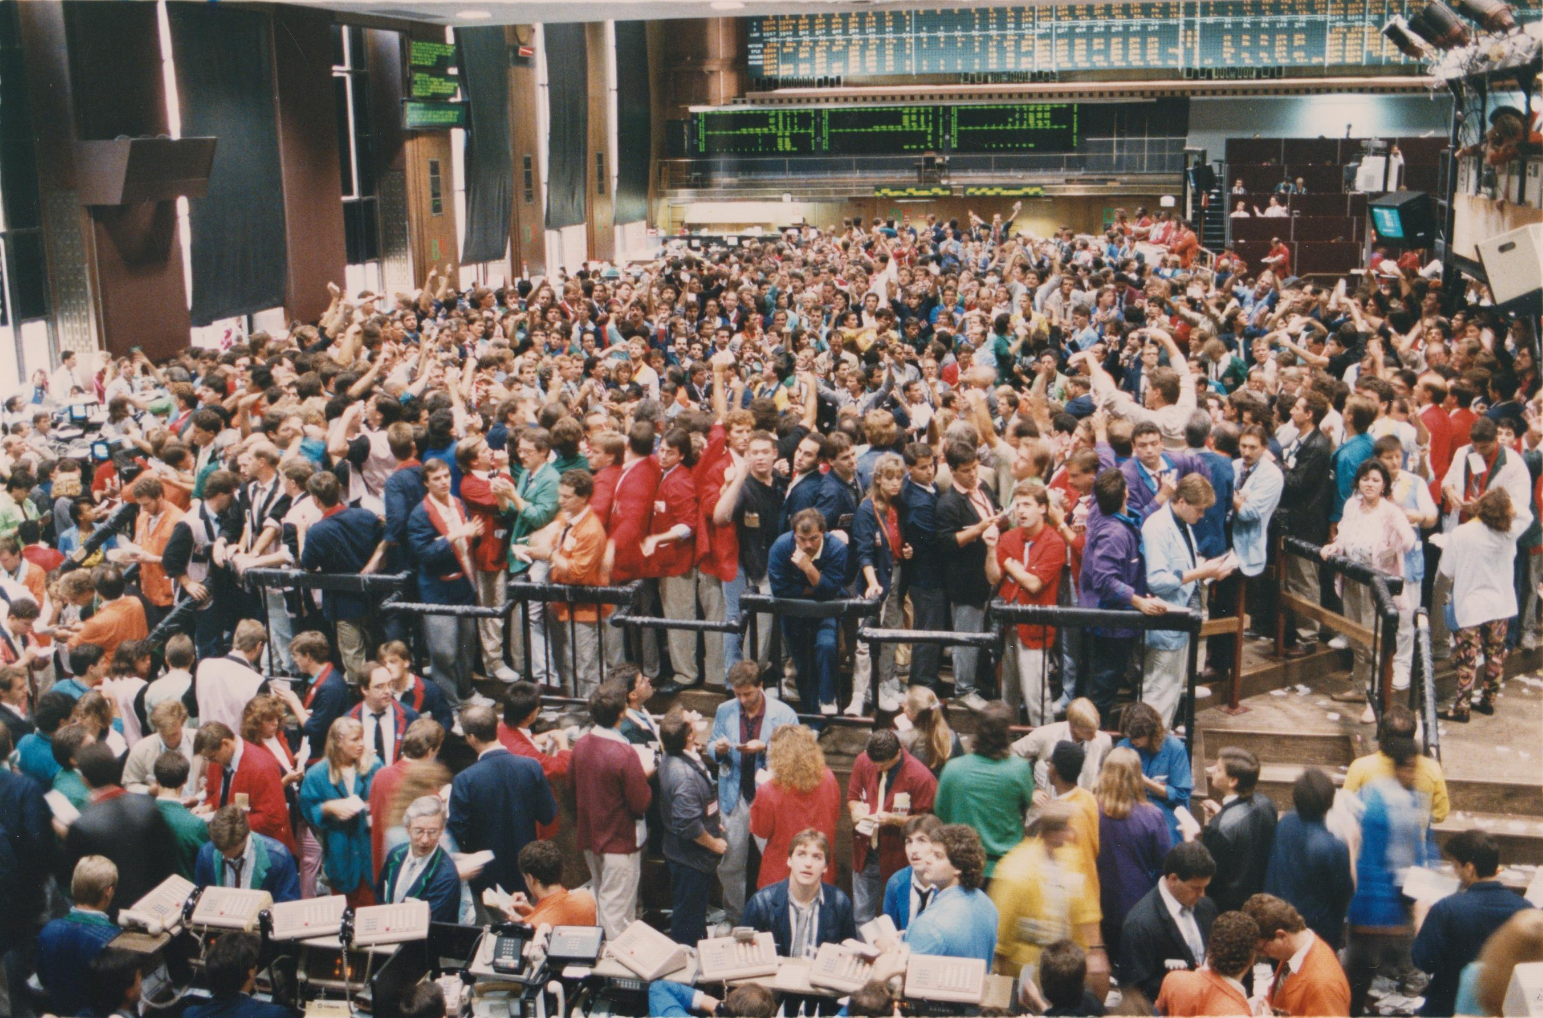
\includegraphics[width=0.9\textwidth]{chapters/chapter_trading_fund/figures/pit_trading.png} 
   	\caption{Treasury bind pit 1989. \label{fig:pittrade}}
	\end{figure}
	\begin{figure}[!ht]
	   \centering
	   \includegraphics[width=0.9\textwidth]{chapters/chapter_trading_fund/figures/electronic_trading.png} 
	   \caption{The NYSE trading floor in August 2008. \label{fig:electrade}}
	\end{figure}
This has also changed how stock market trading is done. The Electronic Communication Networks (ECN) automate the trading process but the fundamental functions of trading are not changed except for the instant dissemination of the demand and supply information to all investors. The identity of traders is kept anonymous. Executions are done fast and very complex orders can now be submitted to the market. The trading costs---both direct such as commissions, brokerage fees, etc. and indirect cost due to price-impact---are expected to be lower. Over the period of two decades (1980--2000), the commissions have have gone down from 1.2\% to 0.2\%. But with higher turnover and thus with increased volume, the total commissions have increased four-fold. The reduction in bid-ask spread although may be primarily due to tick size is accelerated under electronic trading. 


It must be observed that electronic trading does not necessarily imply automated trading. But it has certainly led to more automated trading due to easy execution of the algorithms. Although there is a concern that the traders can game the prices, but computer audit trails can be used to monitor unlawful behaviors. The debate over whether electronification of trading will lead to more consolidation or fragmentation has favored the latter. The apprehension over the possibility of inefficient price formation due to fragmentation is empirically shown not to hold. The order protection rule (SEC 2005) that dictates that an order submitted to any market should get the best of prices in all markets. 


Thus large number of equity and derivative markets are now organized as electronic limit order books. The Electronic Communications Networks (ECNs) in the United States, Hong Kong and Toronto Stock Exchanges are examples of equity markets. Chicago Mercantile Exchange's (CME) Globex platform, Euronext Liffe's centralized limit order book are example of derivative markets. Open limit order books have become popular due to the greater transparency of the market when compared with dealer market settings, that rely upon the information on the dealers' best quotes. The limit order book provides its users to view the depth of the book at various price level away from the best quotes. In dealer market prices for trades beyond the quoted size must be obtained through negotiation with market maker. 


There has been a great deal of interest in studying the information content of an open limit order book and if it helps investors in tracking short-term price predictions. Assuming that the market consists of informed and noise traders, and the informed traders actively submit market orders, Glosten (1994)~\cite{glosten94} and Seppi (1997)~\cite{seppi97} argue that the order book does not contain any information beyond the best bid and best offer. But other studies such as Harris and Panchapagesan (2005)~\cite{harrispan} argue that the order book is informative and specialists better use the book information to their advantage than the traders who routinely place limit orders. In this chapter we discuss the feature of limit order book and various levels of information that have been made available to the investors; the focus is on developing models for studying the dynamics on the book and how the models could be used for high frequency trading. 


An excellent survey paper by Parlour and Seppi (2008)~\cite{parseppi} reviews the issues related to limit order markets. A limit order for any asset `$j$' is an  ex ante pre-commitment $(t,x,p)$ made at time `$t$' to trade `$x$' units at a pre-specified limit price, `$p$'. The order remains valid until it is filled or cancelled. With multiple exchanges, the interactions are quite complex; the dynamic nature of state of the order book and the choice of actions in anticipation of the future states make the limit order placement decisions, $(t,x,p)$ challenging. The key issues in the study of LOB are nicely summarized in Parlour and Seppi (2008)~\cite{parseppi}. They relate to, Price Formulation (How limit order markets differ from dynamic dealer markets?), Liquidity (Implication of the quotes posted at various depths in LOB), Dynamics (Dependencies of Various Trading Decisions), Information Aggregation (How forward-looking is the activity in LOB about future order flow in aggregate?) and Inter-Market Competition (How effective are limit order markets to induce competition and how they handle non-market frictions?). How multiple exchanges can sustain competitive pressure to attract postings to their venues? How do limit order markets help reduce market frictions? These issues are addressed in this chapter but our focus is always on how the information flow through LOB dynamics helps trading decisions. The tools we review here in this chapter can be useful to that end. 


\section{Market Structure and Trading Venues: A Review}
\section{The Mechanics of Trading: The Limit Order Book}

In automated continuous double auction trading system that have have become prevalent in the financial markets, buyers and sellers submit limit orders electronically; orders are then matched and executed as per time and price priorities. The unmatched orders are stored in the limit order book (LOB). The market orders are orders seeking the best available price and they are execute immediately. Thus, one way or other all executed orders can be taken as market orders.


The state of the order book changes quite rapidly due to high frequency program trading. There are six types of events, three on either side that can alter the state of the order book:
	\begin{itemize}
	\item Limit order submission: A limit order is added to the queue at the specified price level.
	\item Limit order cancellation: An outstanding limit order is expired or cancelled and therefore is removed from the LOB.
	\item Market order submission: Outstanding limit order at the best price are executed against the market order and thus removed from the book.
	\end{itemize}


Orders on the buy side are called ``bids'' while those on the sell side are called ``asks.'' The above events illustrated in the following diagrams.
	\begin{figure}[!ht]
	   \centering
	   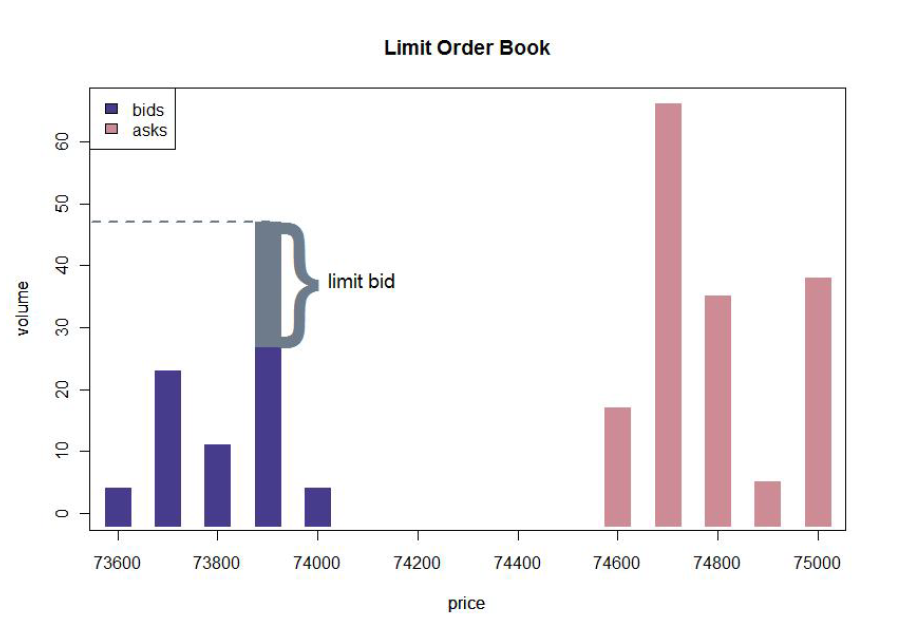
\includegraphics[width=0.9\textwidth]{chapters/chapter_trading_fund/figures/limitbk1.png} 
	   \caption{Limit Order Book---Limit Bid. \label{fig:limbk1}}
	\end{figure}
	\begin{figure}[!ht]
	   \centering
	   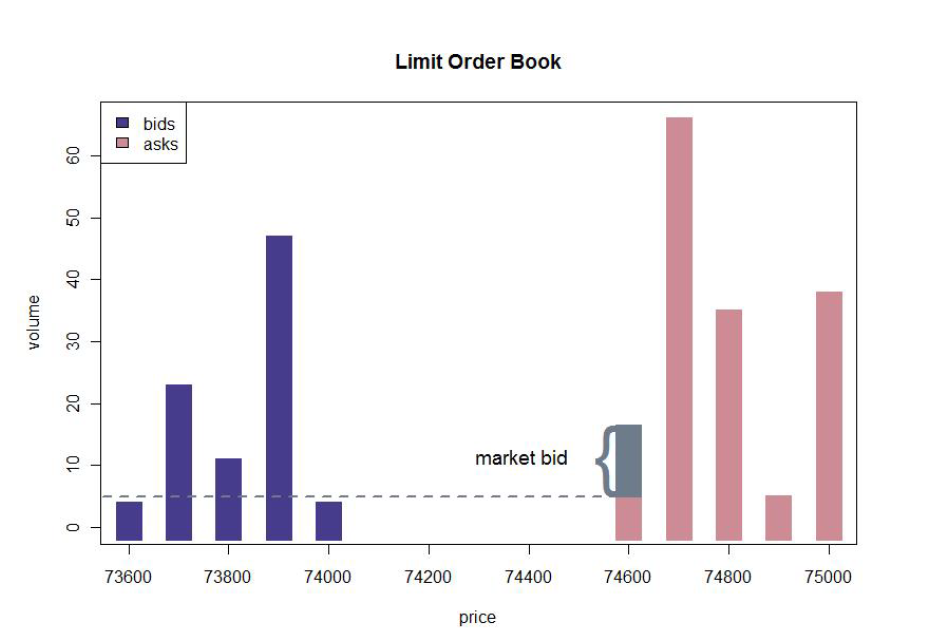
\includegraphics[width=0.9\textwidth]{chapters/chapter_trading_fund/figures/limitbk2.png} 
	   \caption{Limit Order Book---Market Bid. \label{fig:limbk2}}
	\end{figure}
When a market order is submitted, it decreases the number of outstanding orders at the opposite best price. For example, if a market bid order arrives, it will decrease the number of outstanding asks at the best price.
	\begin{figure}[!ht]
	   \centering
	   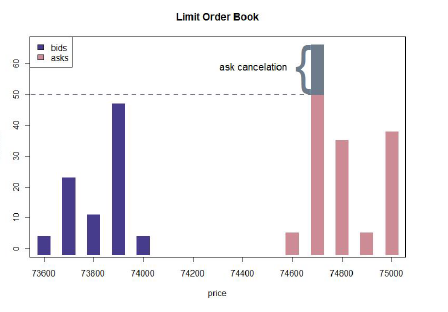
\includegraphics[width=0.9\textwidth]{chapters/chapter_trading_fund/figures/limitbk3.png} 
	   \caption{Limit Order Book---Ask Cancellation. \label{fig:limbk3}}
	\end{figure}
All unexecuted limit orders can be cancelled. When a cancellation occurs, it will decrease the number of outstanding orders at the specified price level. 


The limit orders constitute a very significant percentage (70\%) of stock market trading activity. The main advantage of a limit order is that there is no price risk, that is when the order is executed the limit price is attained. But the execution is not guaranteed and the time to get an order executed depends on various market factors. The trade off between the limit order and the market order depends on the investors need for liquidity and the probability of execution of a limit order. The execution of limit orders does affect how the quotes are posted and are updated. A market order will be filled at or close to National Best Bid and Offer (NBBO). If the size of the order exceeds the number of shares available, it is usually split and is executed at different prices until the order is filled. The market orders are usually restricted to be filled within a day and order placed after the markets close are entered the next day at 9:30~am EST. Other types include stop-limit orders and trailing stop orders. The former type is typically used to trade a security at a specified limit price once it is traded through a specified stop price. If the stock declines in value and traders below or at the stop price, the order will become a limit order rather than a market order. The trailing stop order is in which the specified price will trail by a certain percentage from the best bid or best ask. These rules are handled in the brokers IT technology. In addition to time and duration specifications, other conditions that can be added are: fill or kill (the order gets filled in its entirety or not filled at all) or minimum quantity (if the specified minimum is not available, the order does not get executed).  

\subsection{How Double Auction Markets Work}
\subsubsection{Order Types}
\subsubsection{The Open Auction}
\subsubsection{Continuous Trading}
\subsubsection{The Closing Auction}
\subsection{Market Data}

Initially researchers studying the dynamic of LOB had to content with Trades and Quotes (TAQ) data which provide a time-stamped sequence of trades (Market Orders) and updates in the price and depth of bid and ask quotes. No other information beyond the best bid and the best offer are made available. Moreover, the updates contain changes at the two quotes and were aggregated. The aggregation was clearly a limiting factor as one could not discern the kind of events that led to the changing status of the book. The level II data that became available is a time-stamped sequence of trades and quotes for the top 5-levels of the LOB. This data is little deeper than TAQ data, but was still in aggregated form. But recently made available level III data contains time-stamped sequence of all (except for hidden orders) events that occur in the LOB. Every order is identified by a unique order-id and thus it can be tracked to its lifetime. \\


\noindent\textbf{Description of Level III data:} The dataset consist of activities during the entire trading session, including early and late hours from 6:00~A.M. to 8:00~P.M. EST in a trading day. It provides intraday depth book activity for 12000 tickers from major national exchanges: Nasdaq, Direct Edge, NYSE, ARCA and BATS (exact number of exchanges depends on the historical period). All messages are consolidated into one file ordered by timestamp. This data allows to build a full national depth book at any moment intraday. The description of the level III data is given in Table~\ref{tab:level3data}. \\
	\begin{table}[!ht]
	\centering
	\begin{tabular}{lp{0.8\textwidth}} \hline
	Variable & Description \\
	& \\
	Timestamp: & Number of milliseconds after the midnight. \\
	& \\
	Ticker: & Equity symbol (up to 8 characters) \\
	& \\
	Order: & Unique order ID. \\
	& \\
	T & Message type. Allowed values: \newline \begin{minipage}[t]{0.6\textwidth} \begin{itemize} \item ``B''---Add buy order \item ``S''---Add sell order \item ``E''---Execute outstanding order in part \item ``C''---Cancel outstanding order in part \item ``F''---Execute outstanding order in full \item ``D''---Delete outstanding order in full \item ``X''---Bulk volume for the cross event \item ``T''---Execute non-displayed order \end{itemize} \end{minipage} \\
	& \\
	Shares & Order quantity for the ``B'', ``S'', ``E'', ``X'', ``C'', ``T'' messages. Zero for ``F'' and ``D'' messages. \\
	& \\
	Price & Order price, available for the ``B'', ``S'', ``X'' and ``T'' messages. \newline Zero for cancellations and executions. The last 4 digits are decimal digits. The decimal portion is padded on the right with zeros. The decimal point is implied by position; it does not appear inside the price field. Divide by 10000 to convert into currency value. \\ 
	& \\
	MPID & Market Participant ID associated with the transaction (4 characters) \\
	& \\
	MCID & Market Center Code (originating exchange---1 character) 
	\end{tabular}
	\caption{Level III data \label{tab:level3data}}
	\end{table}
	

\noindent\textbf{Special types of orders:} While the display and issuance of new ID to the modified order varies from exchange to exchange, we provide a brief description of these orders below:

\begin{enumerate}[1.]
\item Order subject to price sliding: the execution price could be one cent worse than the display price at NASDAQ; it is ranked at the locking price as a hidden order, and displayed at the price one minimum price variation (normally 1 cent) inferior to the locking price. New order ID will be used if the order is replaced as a display order. At other exchanges the old order ID will be used.

\item Pegged order: Based on NBBO, not routable, new timestamp upon re-pricing, display rules vary over exchanges.

\item Mid-point peg order: Non-displayed, can result in half-penny execution.

\item Reserve order: displayed size is ranked as a displayed limit order and the reserve size is behind non-displayed orders and pegged orders in priority. The minimum display quantity is 100 and this amount is replenished from the reserve size when it falls below 100 shares. A new timestamp is created and the displayed size will be re-ranked upon replenishing.

\item Discretionary order: displayed at one price while passively trading at a more aggressive discretionary price. The order becomes active when shares are available within the discretionary price range. Ranked last in priority. The execution price could be worse than the display price.

\item Intermarket sweep order: order that can be executed without the need of checking the prevailing NBBO.  
\end{enumerate}


Some key measures of the LOB are: relative position of an order from the top position of the side (buy or sell), the depth which is the total number of shares at a given price and the depth profile of the book reflects the depth of both prices. Large market orders can shift the bid and ask prices. If the limit price of a new order crosses the best price on the opposite side of the book, it is executed immediately and these are termed as crossing or marketable limit orders. These are used at times to explore the existence of hidden orders.


The limit order book data provides a rich source of information to better understand the market microstructure. The information is also useful for developing trading strategies. Some key issues that may be explored are:

\begin{itemize}
\item The pattern of inter-arrival times of various events.
\item Arrival and cancellation rates as a function of distance from nearest touch price.
\item Arrival and cancellation rates as a function of other available information, such as in the queue on either side of the book.
\end{itemize}

The key issues from the trading point of view are:

\begin{itemize}
\item What is the impact of market order on the limit order book?
\item What are the chances for a limit order to move up the queue from a given entry position?
\item What is the probability of making the spread?
\item What is the direction of the price movement in short duration?
\end{itemize}
\subsubsection{Reference Data}
\subsubsection{Daily Statistics}
\subsubsection{Level 1: Trade, Quotes, BBO and NBBO}
\subsubsection{Level 2: Market Depth}
\subsubsection{Level 3: Orders}

\section{The Dynamics of Trading: Market Micro-structure}
\section{Execution and its components}
\subsection{Benchmarks}
\subsection{Scheduling}
\subsection{Order Placement}
\subsection{Order Routing}



\part{Foundations: Basic Models and Empirics}
% !TEX root = ../../../book.tex

In Part I, our goal is to provide a review of some basic and some advanced statistical methodologies that are useful for developing trading algorithms. We begin with time series models (in Chapter 2) for univariate data and provide a broad discussion of autoregressive, moving average models---from model identification, estimation, inference and to model diagnostics. The stock price and return data do exhibit some unique features and so we identify certain stylized facts that have been confirmed; this work will greatly help to discern any anomalies as and when they arise as these anomalies generally indicate deviation from efficient market hypothesis. Wherever possible we illustrate the methodology with examples and provide codes for computing and make the data accessible to the reader. This chapter is followed by methodologies for multiple time series data and the discussion in Chapter 3 is useful from pairs trading to portfolio optimization. The last chapter (Chapter 4) in Part I contains advanced topics such as theory of point processes as trading takes place on a continual basis and understanding the market macro-structure is essential for deciding about the entry to and exit from the market. This chapter also contains other modern topics such as machine learning and artificial intelligence. 


A reader with strong statistics background can afford to skip some sections but it is recommended that the readers peruse these chapters as they contain discussion on topics that need further research work. In presenting the methodologies here, we kept the discussion lucid but immensely relevant to the main theme of this book---understanding the market behavior and developing effective trading strategies. 









% !TEX root = ../../book.tex

\chapter{Univariate Time Series Models}

With the advent of electronic trading a vast amount of data on orders is now recorded and is available to traders to make real-time decisions. The Trades and Quotes (TAQ) data on time-stamped sequence of trades with the updates on the price and depth of the best bid and ask quotes was used by researchers and traders initially. This was later expanded to the so-called Level II data, with time-stamped sequence of trades and quotes for the top 5 levels of the order book. Both TAQ and Level II data still do not provide the complete story of the buy and sell sides. With Level III data now available, we can obtain time-stamped sequence of all events that occur, with the exception of the information on hidden orders. Thus the data related to all trading activities is quite voluminous and is irregularly spaced. We take a broad view that for making strategic decisions to enter and exit the market, the trader needs to take an aggregate view of the trading activities, but that for the actual execution of the strategies the trader needs to understand the market micro-structure that relates to the actual process of trading. With the increased speed of decisions that are made nowadays the difference between the two steps may be blurred, but the aggregation process may help to look beyond trading fractions. In Section 2.1 we discuss the Trades and Quotes data and the aggregation issues. In Section 2.2 we define that the trading algorithms depend on prediction of short-term price movement.


The movement whether it is due to pure market frictions or due to information related to a stock is captured through a drift term that needs to be carefully monitored. Because time series models for discrete time units are well-studied and are still widely used by the traders in the form of aggregated price-bars, we focus on these methods in Sections 2--3 to 2.6. We broadly classify these methods into modeling the mean (return) and into modeling the variance (volatility). As these techniques are well-documented and can be found elsewhere, we only present a brief overview. The established facts about the stock returns and variances are reviewed along with the methodology as these will provide expected benchmarks; successful algorithms as one would notice, generally exploit the deviations from these benchmarks.


In Section 2.7, the time series models are augmented with other stock-related information such as volume. The flow of volume is taken to provide indirectly the flow of information about a stock. As trading now is taking a portfolio point of view, it is important to study multiple stocks together and discrete multiple time-series models provide a framework and these are presented in Section 2.9. Models that deal with the print-processes and the high-frequency analytical tools are covered in the rest of the chapter. 


\section{Trades and Quotes Data and their Aggregation: From Point Processes to Discrete Time Series}


In its simplest form, the trading activities of equity through an exchange that opens at 9:30~a.m. and closes at 4~p.m. can be described by a sequence of time stamps (``ticks'') $t_0 < t_1 < \cdots < t_n$ and the ``marks'' $y_i$ at time $t_i$, in which $t_0$ denotes 9:30~a.m. and after and $t_n$ denotes the time of the last trade that occurs before or at 4~p.m. The marks $y_i$ can be price, volume of an order placed on either the buy or sell side of the trade and in general can represent the characteristics of the order book at the time of $i$th activity (see Figure~\ref{fig:tradeactline}). The events with the marks associated with the ticks can be described mathematically by a marked point process. But our goal here is to first show how these data can be aggregated over regularly spaced time intervals and methods for linear homogeneous time series will be described to analyze the aggregated data and later some tools that are relevant for the analysis of point processes will be presented.


The typical level III data for CISCO on a single day in 2011 is given below in Table~\ref{tab:CISCO}:
% Requires the booktabs if the memoir class is not being used
\begin{table}[!ht]
   \centering
   \caption{CISCO--Trade Data\label{tab:CISCO}}
   \begin{tabular}{cccccc} 
	Timestamp & Order Number & Event & Quantity & Price & Exchange \\ \hline
	$\vdots$ & $\vdots$ & $\vdots$ & $\vdots$ & $\vdots$ & $\vdots$ \\
	34561915 & 4254917 & D & 0 & 0 & J \\
	34561915 & 4253917 & B & 200 & 20.55 & J \\
	$\vdots$ & $\vdots$ & $\vdots$ & $\vdots$ & $\vdots$ & $\vdots$ \\
	34561923 & 13056048 & S & 200 & 20.58 & Z \\
	$\vdots$ & $\vdots$ & $\vdots$ & $\vdots$ & $\vdots$ & $\vdots$ \\
	34573369 & 13255731 & C & 98 & 0 & Q \\
	$\vdots$ & $\vdots$ & $\vdots$ & $\vdots$ & $\vdots$ & $\vdots$ \\
	34577331 & 6225085 & E & 300 & 0 & K \\
	$\vdots$ & $\vdots$ & $\vdots$ & $\vdots$ & $\vdots$ & $\vdots$ \\
	34577338 & 6225085 & F & 0 & 0 & K \\
	$\vdots$ & $\vdots$ & $\vdots$ & $\vdots$ & $\vdots$ & $\vdots$ \\
	34573379 & 2030057 & S & 100 & 20.77 & K \\
	$\vdots$ & $\vdots$ & $\vdots$ & $\vdots$ & $\vdots$ & $\vdots$ \\
	34573382 & NA & T & 1700 & 20.37 & P \\
	$\vdots$ & $\vdots$ & $\vdots$ & $\vdots$ & $\vdots$ & $\vdots$ 
   \end{tabular}
\begin{minipage}[t]{1\textwidth}
\small{*Time-stamp is the time since midnight; Event: B: submission of LO on Buy side; S: submission of LO on sell side; T: full execution of a LO; F: full execution of a LO; E: partial execution of a LO; D: full cancellation of a LO; C: partial cancellation of a LO; Exchange: Q-NASDAQ; J-EDGE-A; Z-BATS-Z; K-EDGE-K; P-ARCA; etc}
\end{minipage}
\end{table}


This outlay in Table~\ref{tab:CISCO} points to various issues that need to be addressed in processing this type of data. The order numbers are only unique during the lifetime of the order but can be reassigned at a later time. Several activities can take place at the same time. Hidden orders are revealed only when they are executed and as such do not have visible order numbers. Full cancellation quantity and price information should be traced back to the submission time. To summarize, at any given point in time using the data described in Table~\ref{tab:CISCO}, limit order book that essentially records where the order is in the queue, can be constructed and thus providing the trade time and the associated marks. These and other characteristics of the limit order book (superbook---if we collate this information from all exchanges) will be taken up in a later chapter, but the focus here is on constructing discrete time series data from this point process data. 


To illustrate the aggregation methods, we will initially focus on price of the stock, $p_t$, and the associated volume $V_{t}$. Two types of aggregation methods are proposed in the literature. One when the time span $T$ for the Exchange hours (9:30~a.m.--4:00~p.m.) is divided into `$K$' intervals so that the regularly spaced intervals are of size $\Delta t = T/K$. The other method will do aggregation when there is a change in a marker, such as price. Here we focus on the first method. Various summary measures within each period $((i - 1)\Delta t, i\Delta t)$ where $i = 0,1,\ldots,K$ can be computed;
\begin{itemize}
\item number of transactions: `$n_i$'
\item Average price: $\overline{p}_i = \sum p_{t_j}/n_i$
\item Volume Weighted Average Price: $\overline{p}_{wi} = \sum V_{t_j}p_{t_j}/\sum V_{t_j}$
\item Average duration between transactions: $\overline{d}_i = \sum_{j\in ((i-1)\Delta t,i\Delta t) }(t_j - t_{j-1})/n_i$
\item Mid-Price: $(\text{Best bid}+\text{Best ask})/2$
\end{itemize}


It is possible that for infrequently traded stocks, some time intervals may not contain any trading activity. For heavily traded stocks, the duration can be very small and thus may not provide any consequential information. We will address ways to analyze high-frequency data later in this chapter. To begin with, we discuss the analysis for data aggregated over fixed time intervals. Depending on the size of the interval, the data can be called low frequency or high frequency but the time series methods that we discussed here apply to \textit{all} aggregated data.
	\begin{figure}[!ht]
	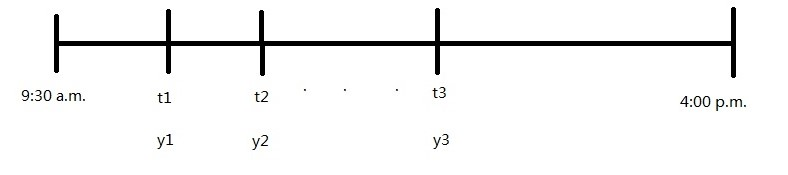
\includegraphics[width=4in]{chapters/chapter_uvts/figures/33d1.jpg}
	\caption{Trading Activities \label{fig:tradeactline}}
	\end{figure}


\section{Trading Decisions as Short-Term Forecast Decisions} 


Most trading decisions generally involve the following considerations
\begin{itemize}
\item How much to trade?
\item When to trade? ie when to enter and when to exit?
\item How to trade? How fast? What is the objective? What are the benchmarks?
\end{itemize}
Answer to these questions involve in some way predicting the market movement and in particular the future (short-term and long-term) price of assets. In the short term it is possible that prices have a tendency to `trend' or exhibit `momentum' but in the long run, prices have a tendency to `mean-revert' as the information about the asset gets incorporated in the price. 


Let $p_{it}$ denote the price of the $i$th asset at time $t$ and let $p_t = (p_{1t},p_{2t},\ldots,p_{nt})$ denote the price vector for `$n$' assets. Let $y_{it}$ denote a vector of characteristics, e.g. volume of transactions, price volatility, number of transactions and the intensity of trading as captured by the average duration between transactions, etc of the $i$th asset at time $t$. These quantities are aggregated from high-frequency data of type given in Table~\ref{tab:CISCO} and illustrated in Figure~\ref{fig:tradeactline} to be used as the characteristics associated with the price changes. In addition, we can also consider factors $f_t = (f_{1t},f_{2t},\ldots,f_{nt})$ that may include market and industry factors as well as asset characteristics such as market capitalization, book-to-market ratio etc. The trading rules can be broadly grouped as follows:
\begin{itemize}
\item[A.] Statistical Arbitrage Rules: $E(p_{i,t+1}\,|\,p_{i,t},p_{i,t-1},\ldots,y_{i,t},y_{i,t-1},\ldots)$
\begin{itemize}
\item[$\bullet$] Predicting the price of $i$th stock at t+1 based on the past trading information; this is sometimes labelled as time series momentum.
\end{itemize}
\item[B.] Momentum: $E(p_{t+1}\,|\,p_{t},p_{t-1},\ldots,y_{t},y_{t-1},\ldots)$
\begin{itemize}
\item[$\bullet$] Predicting the cross-sectional momentum of a subset of stocks based on their past trading characteristics. This is not only useful for portfolio formation and rebalancing, also for pairs trading which is based on tracking two stocks simultaneously so that their divergence can be exploited. 
\end{itemize}
\item[C.] Fair Value: $E(p_{t+1}\,|\,p_{t},p_{t-1},\ldots,V_{t},V_{t-1},\ldots,f_t,f_{t-1},\ldots)$
\begin{itemize}
\item[$\bullet$] Predicting the price using all relevant quantities. Many of these factors can be at a more macro level than the time scale considered for the price prediction, but nevertheless could be useful, as explained in Chapter 3.
\end{itemize}
\end{itemize}
\noindent Thus the price (or alternatively, return) and volatility (or squared return) prediction can be formulated as a time series prediction problem and the common tools such as autoregressive and ARCH models can be used. 


Predicting stock market behavior has been studied extensively starting in the early 20th century. Cowles (1933, 1944)~\cite{cow2,cow1} evaluated the performance of the stock market forecasters. Analyzing the performance of several financial services that made some 7500 recommendations on common stocks over a period, January 1, 1925 to July 1, 1952, it was pointed out the record was worse than the performance of average common stock by 1.43\% annually. Thus `buy-and-hold' strategy out-performed the stock picking strategies of those days. In fact, a much harsher assessment is made: ``A review of the various statistical tests, applied to the records for this period, of these 24 forecasters, indicates that the most successful records are little, if any, better than what might be expected to result from pure chance. There is some evidence, on the other hand, to indicate that the least successful records are worse than what could reasonably be attributed to chance.'' Many of these comments are still valid and have stood the test of the time. Yet, we will demonstrate in this book that there are opportunities for statistical arbitrage. The key is to have access to relevant information and use the appropriate techniques to exploit this in a timely manner. 


\section{Time Series Models for Aggregated Data: Modeling the Mean}

In this section we present a broad overview of the time series models for data aggregated over discrete time intervals. 

\subsection{Stochastic Processes: Some Properties} \hfill

Formally, a discrete time series or stochastic process $Y_1, Y_2, \ldots, \, Y_T$ is a sequence of random variables (r.v.'s) defined on a probability space, and possessing a joint probability distribution, with $Y_t$ denoting the r.v. corresponding to the value of the series at time $t$. A particular sequence of observations of the stochastic process $\{ Y_t, t=1, \ldots,  \, T\}$ is known as a realization of the process. In the analysis of time series we are interested in aspects of the joint probability distribution of collections of random variables such as $Y_1, Y_2, \ldots, \, Y_T$. For such a collection of r.v.'s, the joint distribution function is defined by
	\begin{equation}\label{eqn:feqnfirst}
	F_{12 \ldots T}\left(y_1, y_2, \ldots,  \, y_T\right)= \text{Pr}[Y_1 \leq y_1, Y_2 \leq y_2, \ldots,  	\, Y_T \leq y_T]
	\end{equation}
In general, time series analysis is concerned with determining the properties and identifying the probability structure which generated the observed time series. A general feature of the approach to this analysis is that we do not attempt to study the joint distribution of $Y_1, Y_2, \ldots, \, Y_T$ directly, since this may be too complicated for large $T$, but we study and attempt to describe the probabilistic mechanism which generates the process sequentially through time, and from this to derive the conditional distribution of future observations for purposes of prediction.


Because the means, variances, and covariances are useful summary descriptions of the joint probability distribution of the stochastic process $\{ Y_t, t=1, \ldots,  \, T\}$, we will first consider these quantities. Thus, for any stochastic process $\{Y_t\}$, we define the following functions of $t$:
	\begin{equation}\label{eqn:texteqn}
	\begin{split}
	\text{mean, }\mu(t)&=E(Y_t) \\
	\text{variance, }\sigma^2(t)&=\Var(Y_t)=E[(Y_t-\mu(t))^2] \\
	\text{autocovariance, }\gamma(t,s)&=\Cov(Y_t,Y_s)=E[(Y_t-\mu(t))(Y_s-\mu(s))] \\
	\text{autocorrelation, }\rho(t,s)&=\Corr(Y_t,Y_s)=\dfrac{\gamma(t,s)}{\sigma(t)\sigma(s)}
	\end{split}
	\end{equation}
 Obviously, it is not possible to estimate the many unknown parameters (means, variances, and covariances) under such a general specification from a single realization of $T$ observations. In addition, such generality in the specification of the mean and covariance structure offers no information concerning the prediction of future observations of the process. Hence we must impose some additional structure on the joint distribution of the process in order to substantially reduce the number of unknown parameters, as well as to enable meaningful predictions into the future to be possible. The concept of stationarity of a process is useful in this regard and also serves as a realistic assumption for many types of time series. Stationarity is motivated by the fact that for many time series in practice, segments of the series at different points in time behave similarly, or exhibit homogeneous behavior over time. \\


\noindent \textbf{Stationarity} \\


A time series $\{Y_t\}$ is said to be stationary if for every integer $m$ and any finite set of $m$ time points $t_1, t_2, \ldots, \, t_m$ the set of variables $Y_{t_1}, Y_{t_2}, \ldots, \, Y_{t_m}$ must depend only on the distance between the times $t_1, t_2, \ldots, \, t_m$, rather than on their actual values.  So a stationary process $\{Y_t\}$ tends to behave in a homogeneous manner as it moves through time. The means and variances of the $Y_t$ are the same for all $t$, that is, $E\left(Y_t\right) = \mu$ and  Var$\left(Y_t\right)=\sigma^2$ are constant, for all $t$. So we may express the autocovariance function as 
	\begin{equation}\label{eqn:2gammas}
	\gamma(s)=\Cov(Y_t,Y_{t+s})=E[(Y_t-\mu)(Y_{t+s}-\mu)], \text{ for all }s=0,\pm 1,\cdots
	\end{equation}
Note that by this notation, $\gamma(0) = E[(Y_t-\mu)^2] = \text{Var}(Y_t)$. Also, the \textit{autocorrelation function} of the stationary process may be expressed
        	\begin{equation}\label{eqn:2rhos}
	\rho(s)=\Corr(Y_t,Y_{t+s})= \dfrac{\Cov(Y_t,Y_{t+s})}{\big(\Cov(Y_t)\Cov(Y_t)\big)^{1/2}} = \dfrac{\gamma(s)}{\gamma(0)},  s=0,\pm 1,\cdots
	\end{equation}
$\rho(s)$ will be referred to as the autocorrelation of the process at lag $s$. As we will find, the autocorrelation function (which we will abbreviate as ACF) $\rho(s) = \gamma(s)/\gamma(0)$ of a stationary process $\{Y_t\}$ is a very important tool in describing the characteristics of the process, since it is a convenient summary of the correlation structure of the process over all time lags.  \\


\noindent \textbf{Examples of Stationary Stochastic Processes} 


\begin{ex}[White Noise] \label{ex:whitenoise} Let $\ldots, \epsilon_{-1}, \epsilon_0, \epsilon_1, \ldots$ be a sequence of independent random variables defined on the discrete time points $\ldots,-1,0,1,\ldots$, with mean $E(\epsilon_{t})=0$ and variance $E(\epsilon_{t}^2)=\sigma^2$, for all $t$. Set $Y_t = \mu + \epsilon_t, \, t=0, \pm1, \ldots$. Then $E(Y_t)=\mu$ for all $t$, and since independence implies that the random variables are uncorrelated, we have $\Cov(Y_t,Y_{t+s})=\Var(Y_t)=\sigma^2$ if $s=0$ and $\Cov(Y_t,Y_{t+s})=0$ if $s\neq0$. Thus the process is stationary. Such a process is referred to as purely random process or a \textit{white noise process}, and will be found to be the foundation for the construction of many other processes of interest. 
\end{ex}


\begin{ex}[Moving Average] \label{ex:movingaverage} Let $\{\epsilon_t\}$ be independent r.v.'s as in Example~\ref{ex:whitenoise}, and define a new process $\{Y_t\}$ by
	\[
	Y_t = \mu + \epsilon_t + \epsilon_{t-1}, \qquad t=0, \pm1, \cdots
	\]
where $\mu$ is a constant.  Then $E(Y_t)=\mu$, for all $t$, and
	\[
	\Cov(Y_t,Y_{t+s})=\gamma(s)=
	\begin{cases}
	 2\sigma^2 & \text{if } s=0 \\
	  \sigma^2 & \text{if } s=1 \\
	  0 & \text{if } s>1 \\
	\end{cases}
	\]
which depends only on the time lag $s$ and not on $t$.  Hence the process $\{Y_t\}$ is stationary with ACF $\rho(s)=\gamma(s)/\gamma(0)$ such that $\rho(0)=1$, $\rho(1)=1/2$ and $\rho(s)=0$ for $|s|>1$.
 
            \begin{sidewaysfigure}[hbp] %htbp
                %\centering
                \label{chap2fig2}
                \subfigure[Figure 1a]
                        [Time series plot of $0.5 + \epsilon_t$]
                        {
                        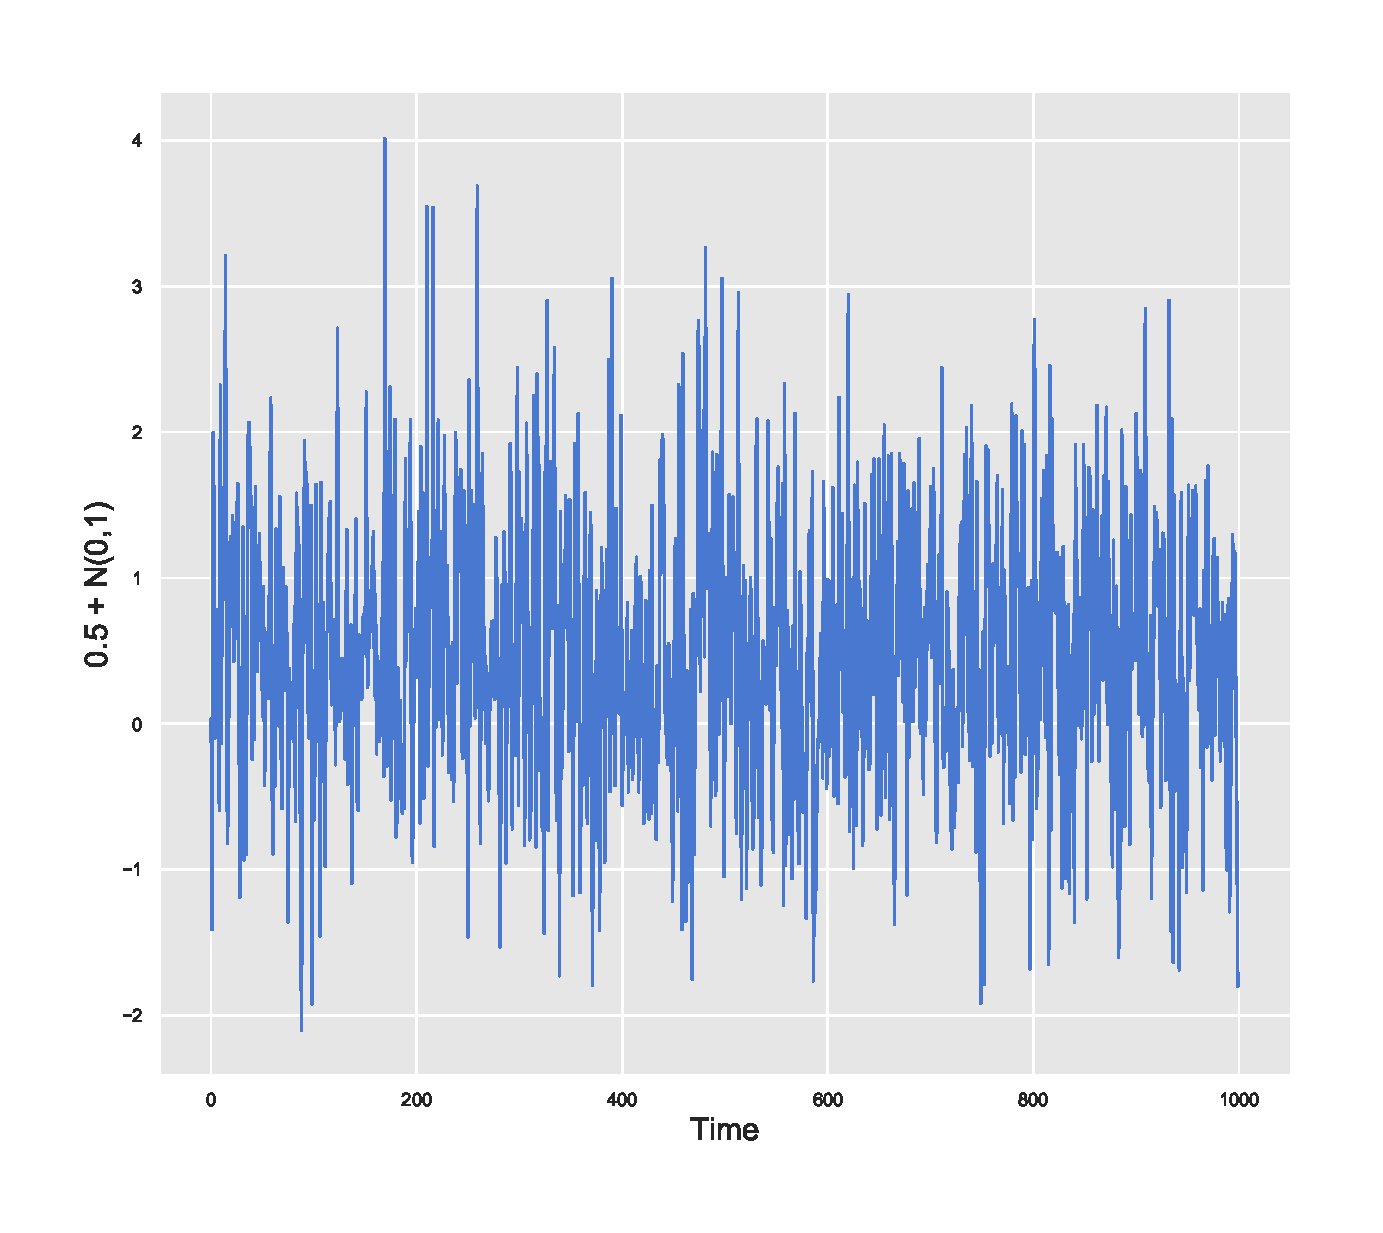
\includegraphics[scale=0.32]{chapters/chapter_uvts/figures/ch1fig1y1ts.eps}
                        }
                        \hfill
                \subfigure[Figure 1b]
                        [ACF]
                        {
                        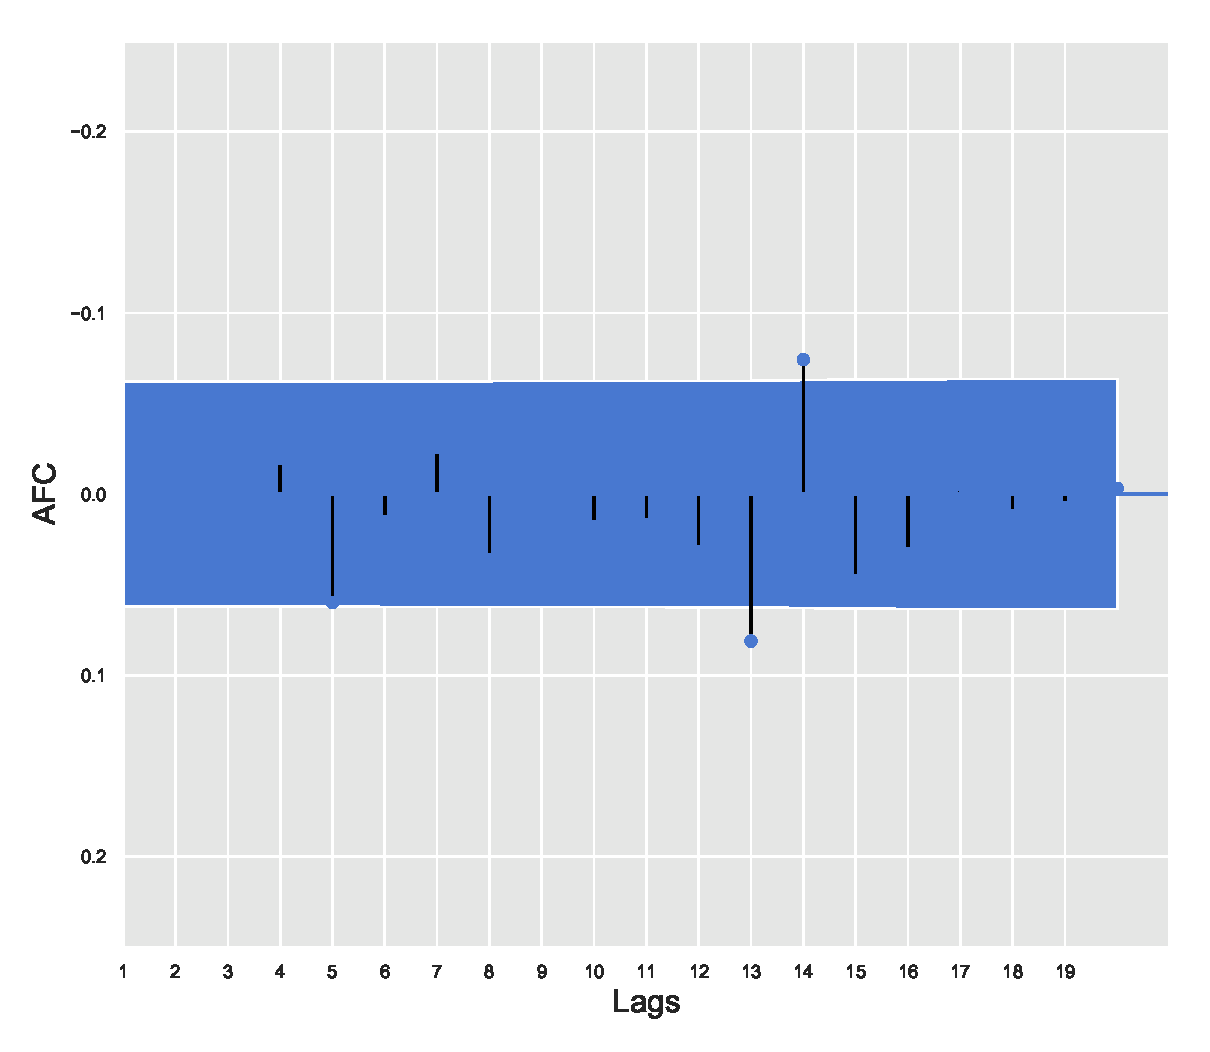
\includegraphics[scale=0.32]{chapters/chapter_uvts/figures/ch1fig1y1acf.eps}

                        }
                        \hfill
                %\subfloat[Figure 1ab][Time Series Plot \& ACF Plot]
                %{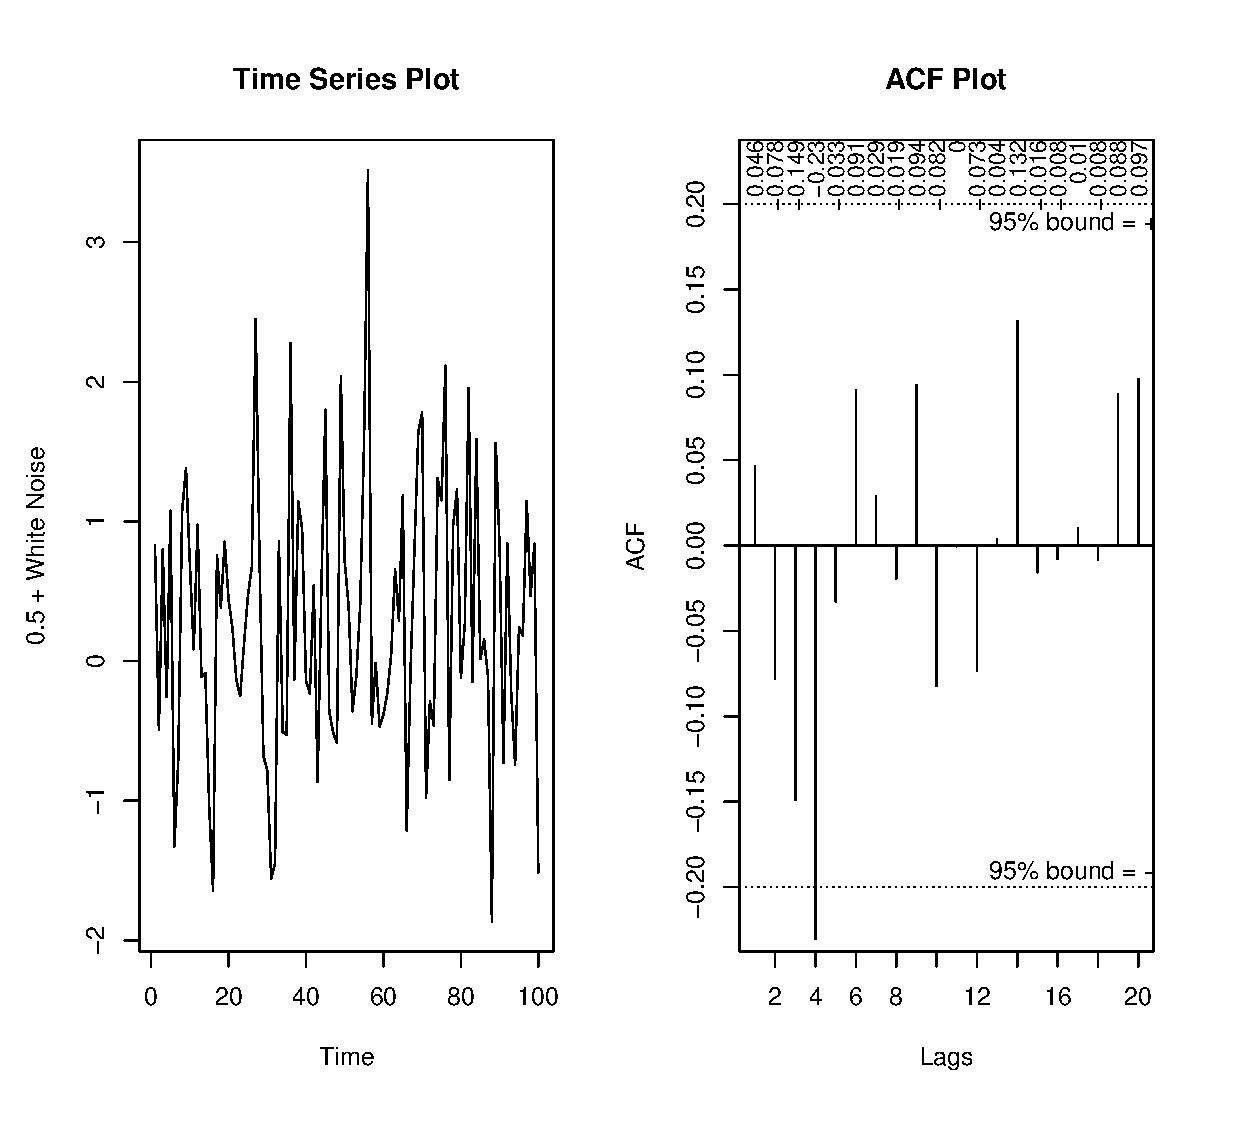
\includegraphics[width=\textwidth, height=0.5\textheight]{ch1fig1y1ab.eps}}
                %\qquad
                \subfigure[Figure 1c]
                        [$Y_t$ vs. $Y_{t-1}$]
                        {
                        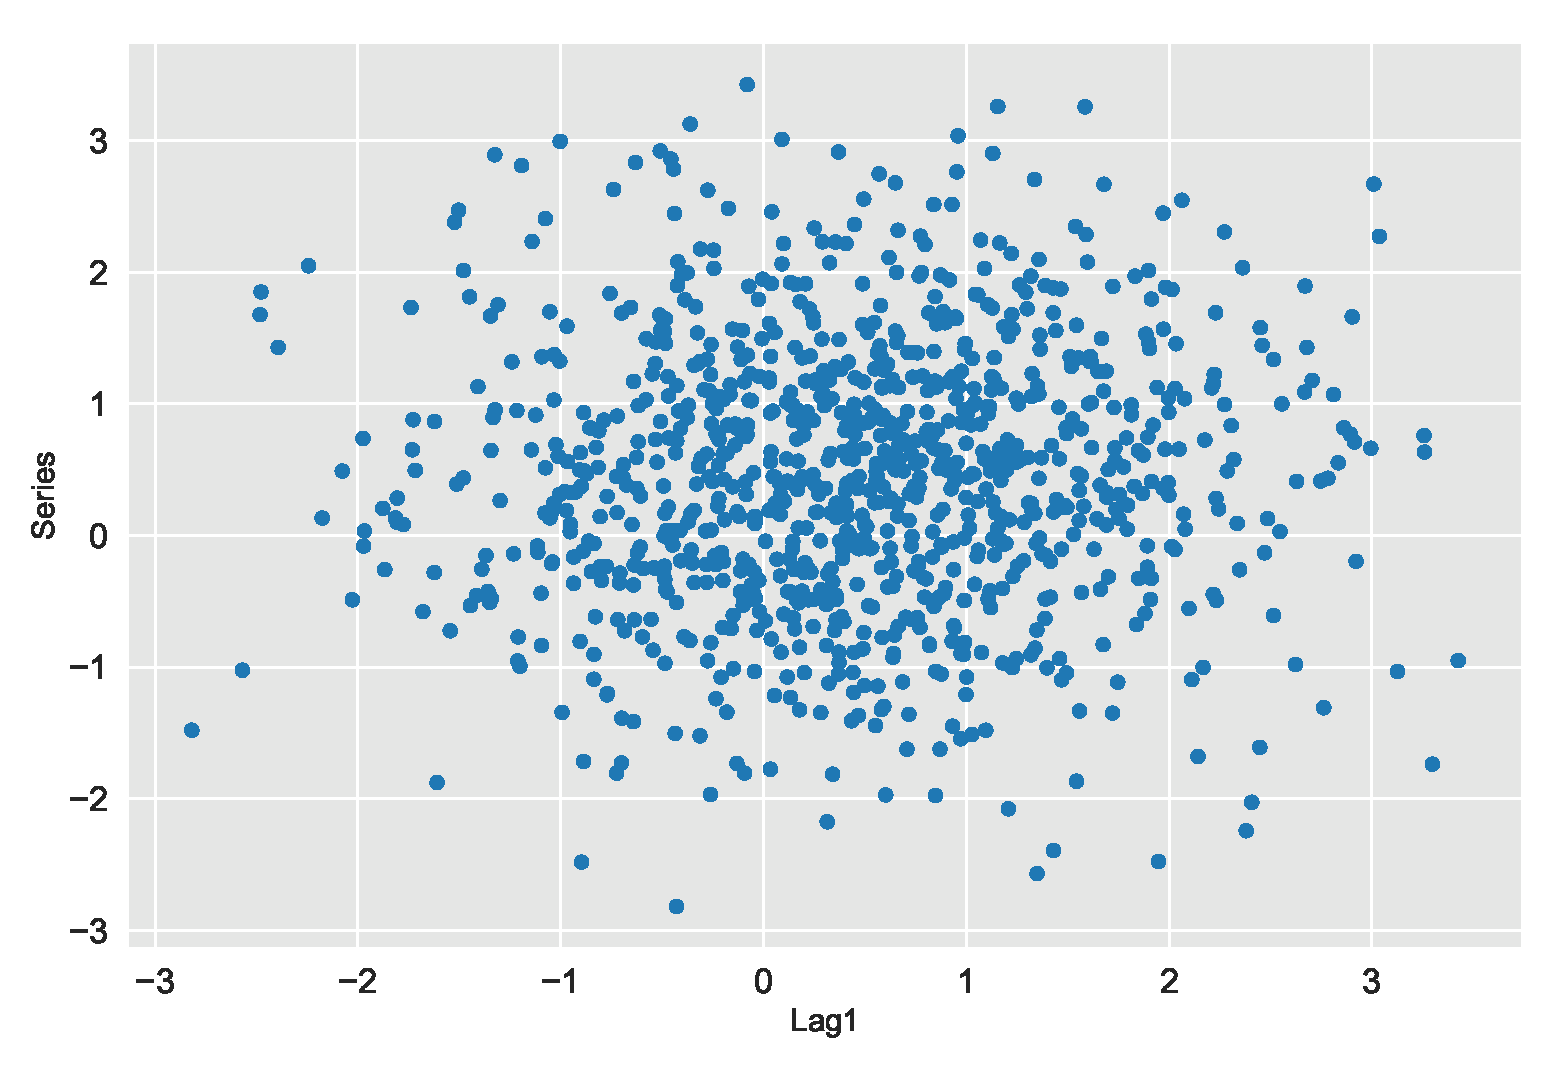
\includegraphics[scale=0.32]{chapters/chapter_uvts/figures/ch1fig1y1lagplot.eps}

                        }
                %%%%%%
                \quad           %\qquad
                %%%%%
                \subfigure[Figure 1d]
                        [Time series plot of $1.0 + \epsilon_t + \epsilon_{t-1}$]
                        {
                        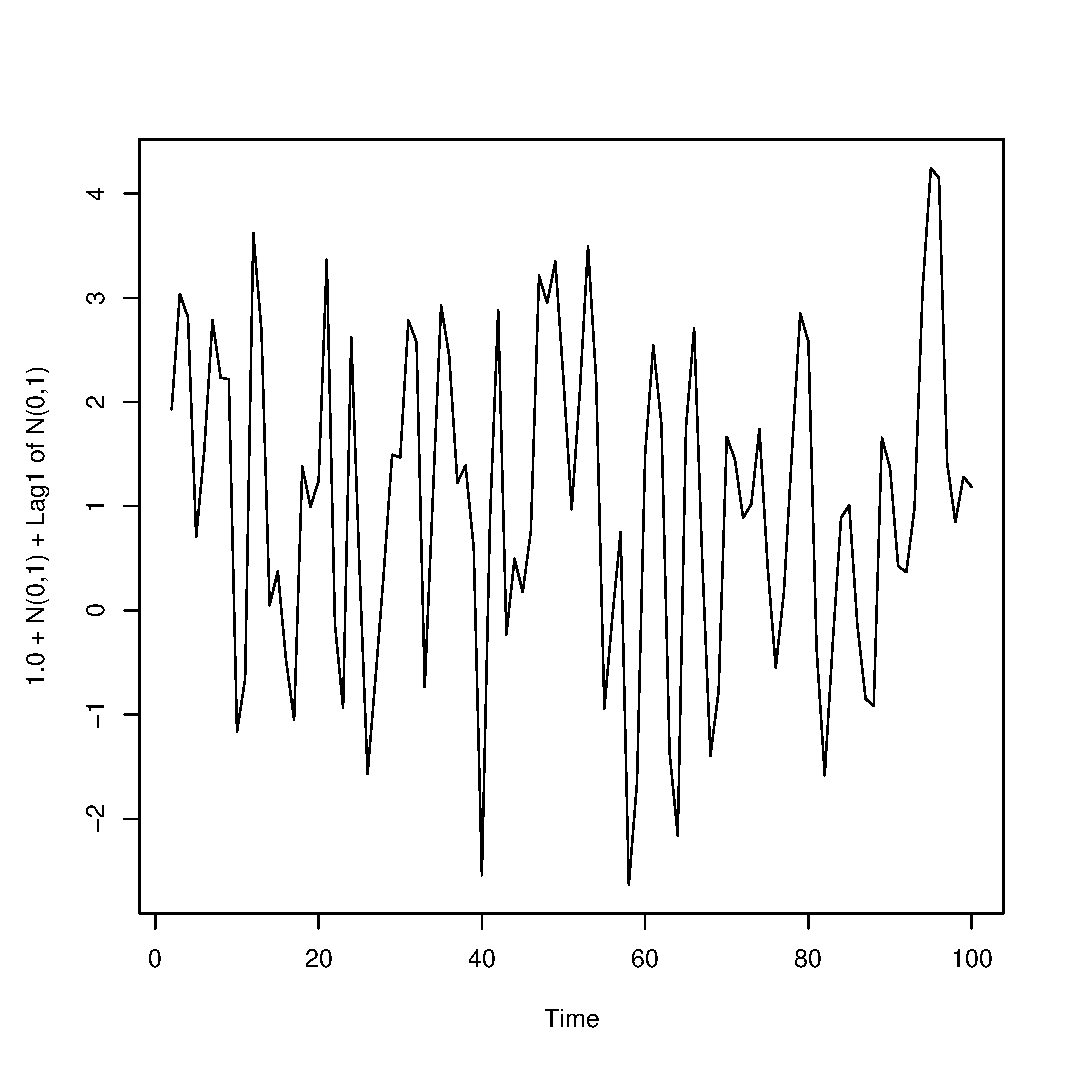
\includegraphics[scale=0.32]{chapters/chapter_uvts/figures/ch1fig1y2ts.eps}

                        }
                        \hfill
                \subfigure[Figure 1e]
                        [ACF]
                        {
                        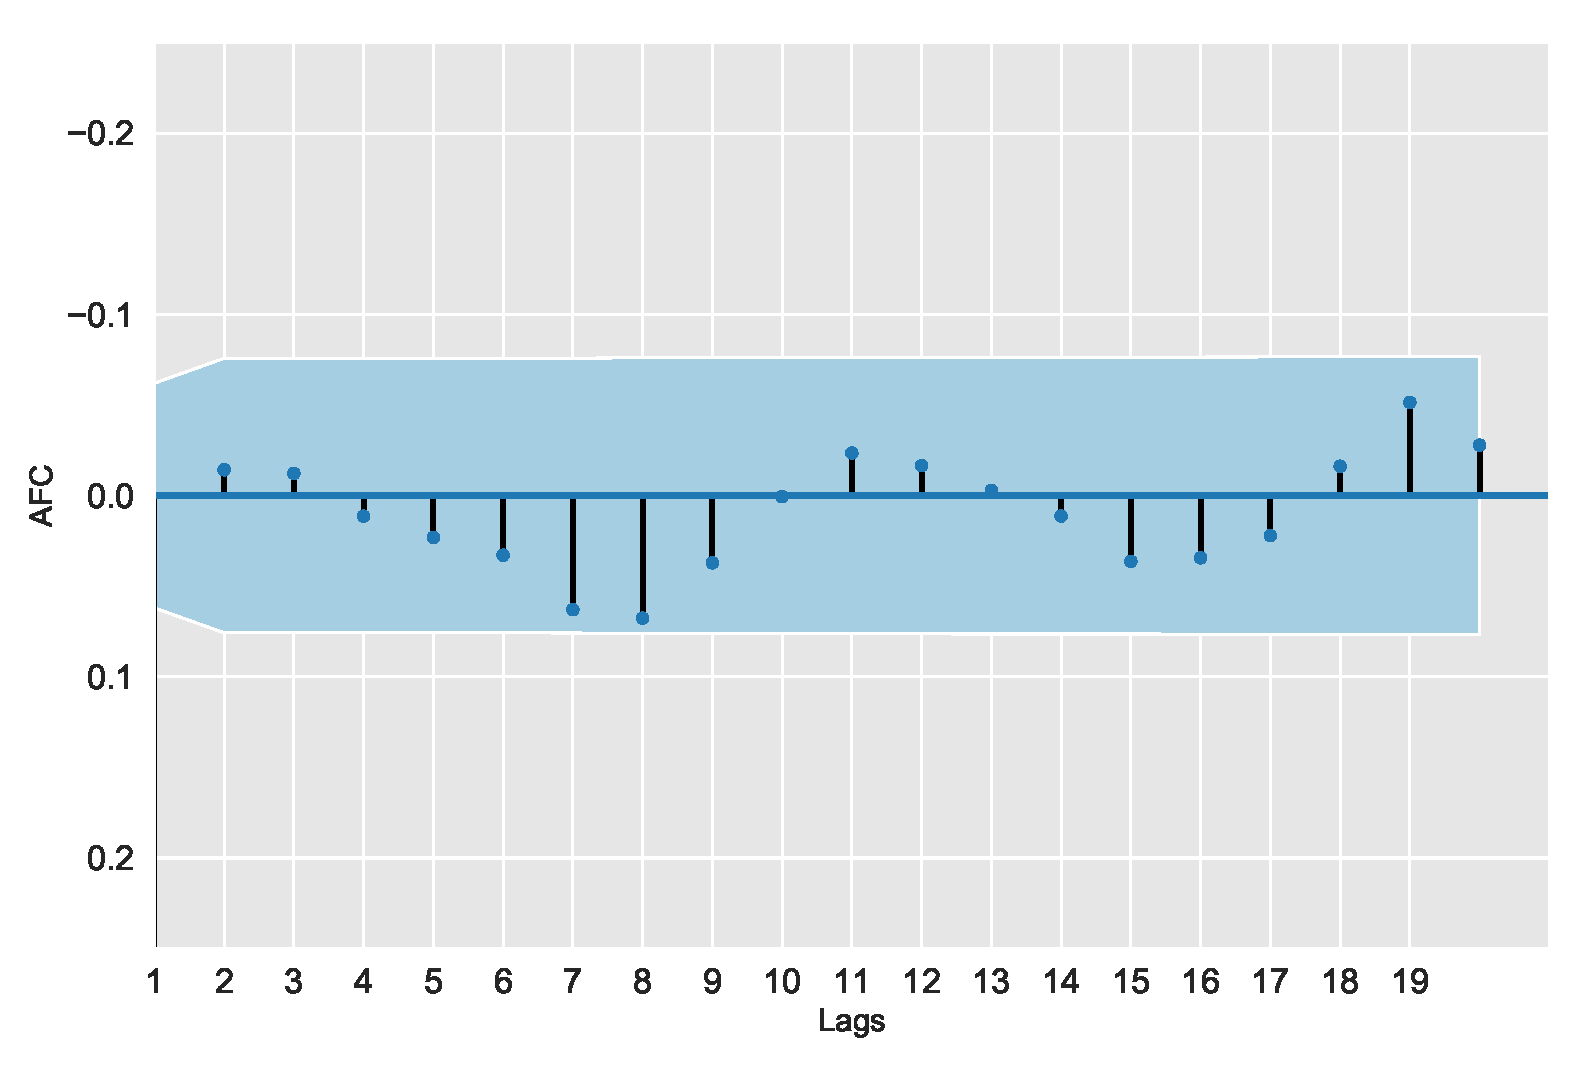
\includegraphics[scale=0.32]{chapters/chapter_uvts/figures/ch1fig1y2acf.eps}

                        }
                        \hfill
                \subfigure[Figure 1f]
                        [$Y_t$ vs. $Y_{t-1}$]
                        {
                        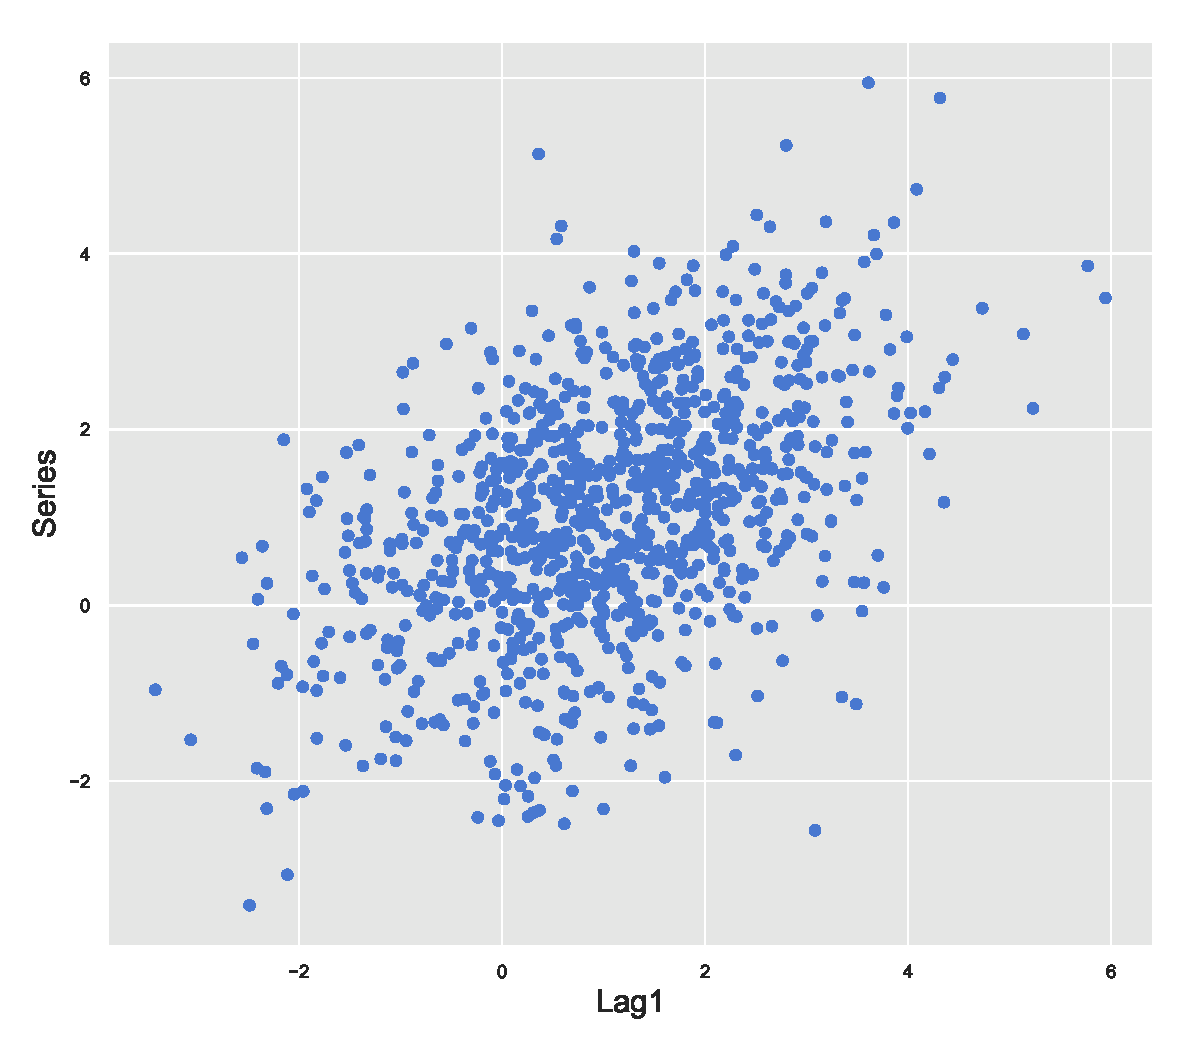
\includegraphics[scale=0.32]{chapters/chapter_uvts/figures/ch1fig1y2lagplot.eps}

                        }
               \caption{Processes \& Diagnostics from $Y_t = 0.5 + \epsilon_t$ and from $Y_t =1.0 + \epsilon_t + \epsilon_{t-1}$\label{fig:sideways}}
            \end{sidewaysfigure}


Figure~\ref{fig:sideways}~(a) shows a time series plot of a computer simulated series of 100 values from a Gaussian white noise process $\{\epsilon_t\}$ with $\sigma^2=1$, while Figure~\ref{fig:sideways}~(b) shows a plot of the corresponding values of the series $Y_t = 1.0 + \epsilon_{t} + \epsilon_{t-1}$ using these same $\{\epsilon_t\}$.  Note the relatively much smoother behavior over time of the data in (b) than in (a), due to the positive autocorrelation at lag one of the process in (b) which tends to make successive values of the series behave more similarly to each other.  Similar to the last example, it is easy to show that the process $\{Y_t\}$ defined by the relation $Y_t = \mu + \epsilon_{t} - \epsilon_{t-1}$ is stationary with autocorrelation function $\rho(0)=1$, $\rho(1)=-1/2$, and $\rho(s)=0$ for $|s|>1$. A plot of a simulated series from this process is given in Figure~\ref{fig:sideways}~(d) where the much ``rougher'' or less smooth behavior over time relative to the behavior  in (a) and (b) due to the addition of extra noise to the model. These figures form the basis of model building and the subsequent diagnostic checks on the fitness of models. 
\end{ex} 


\noindent \textbf{Examples of Nonstationary Stochastic Processes} \\


Many time series that occur in finance do not exhibit stationary behavior.  For example, many stock price series show a trend or change in the mean level over time, reflecting information flow about the stock or investors' behavior. Series also exhibit seasonal behavior, either in the form of nonstationary or deterministic seasonal patterns, both of which need to be distinguished from purely nondeterministic stationary stochastic behavior. Other departures from stationarity include changes in variability of the process over time (nonconstant variance or volatility regimes), abrupt shifts in the mean level, and changes in the autocorrelation structure of the process over time which is a feature of the series which would typically be more difficult to detect.  An important practical matter in the analysis of time series data involves methods of transforming a possibly nonstationary time series into a stationary series, and accounting for and modeling of the nonstationary aspects of the original series.  Many of the methods that are found useful in practice involve considering successive changes or differences over time in the original series to remove the nonstationary features of the series, especially changes in the mean level, or using linear regression techniques to help account for the nonstationary mean behavior.  We will illustrate this with a few simple examples. 


\begin{ex}[Random Walk with a Drift] \label{ex:driftwalk} Let $\{\epsilon_t, \, t=0,1,2, \ldots\}$ be a sequence of independent random variables with mean 0 and variance $\sigma^2$, and define a new process $\{Y_t\}$ recursively by
	\[
	Y_t = Y_{t-1} + \delta + \epsilon_t, \qquad t=0,1,2, \ldots, \quad Y_0 = 0,
	\]
where $\delta$ is a constant.  By successive substitutions in the above relations for $Y_t$, we find that $\{Y_t\}$ can also be expressed as
	\[
	Y_t = \delta \, t + \sum_{j=1}^t \epsilon_j= \delta \, t + \epsilon_{t} + \epsilon_{t-1} + \ldots + \epsilon_{1}, \qquad t=1,2, \ldots .
	\]
Hence we see that $E(Y_t)=\delta t$ and $\Var(Y_t)= \Var(\sum_{j=1}^t \epsilon_j)= \sum_{j=1}^t\Var(\epsilon_j)=t \, \sigma^2$, so that the process $\{Y_t\}$ is not stationary and exhibits change in both mean and variance.  Moreover, for any $s>0$, we find that
	\[
	\Cov(Y_t,Y_{t+s})= \Cov\left(\sum_{j=1}^t \epsilon_j, \sum_{i=1}^{t+s} \epsilon_i\right)= \sum_{j=1}^t\text{Var}(\epsilon_j)= t \, \sigma^2 \, ,
	\]
so that $\Corr(Y_t,Y_{t+s}) = t / \sqrt{t(t+s)} = 1/ \sqrt{1+s/t}$. Note that this correlation is close to one for large $t$ and relatively small $s$, so that nearby values $Y_t$ and $Y_{t+s}$ of the process $\{Y_t\}$ are highly positively correlated.  However, note that the time series of successive changes or \textit{first differences} of the process $\{Y_t\}$, defined by $Z_{t}=Y_{t}-Y_{t-1}$, does form a stationary process, since $Z_{t}=Y_{t}-Y_{t-1} = \delta + \epsilon_t$, a white noise series as in Example~\ref{ex:whitenoise}. Such a process $\{Y_t\}$ whose first differences form a white noise series, is called a random walk process. Time series plots of simulated data from random walk exhibit behavior with little tendency to vary around a fixed constant mean level. The parameter $\delta$ in the random walk model is referred to as the drift in the random walk process. Note the trend behavior in the process with $\delta>0$.
\end{ex}


Of course, a more general class of models is obtained by supposing that a nonstationary process $\{Y_t\}$ is such that its first differences form a stationary process, but not necessarily white noise.  It has been found from practical experience that this type of model is quite useful in producing adequate representations for actual observed financial series in many cases.


\subsection{Some Basic Models and Descriptive Tools} \hfill


Suppose we have a sample realization of $T$ observations $Y_1, Y_2, \ldots, Y_T$ from a stationary process $\{Y_t\}$ which has a mean $\mu=E(Y_t)$, autocovariance function (ACF) $\gamma(s)=\Cov(Y_t,Y_{t+s})$ and autocorrelation function $\rho(s)=\Corr(Y_t,Y_{t+s}) = \gamma(s)/\gamma(0)$. Since the theoretical ACF $\rho(s)$ is such a basic quantity which describes the correlation properties of the process, we are naturally interested in obtaining estimates of $\rho(s)$ from the sample data.


First, a natural estimator of $\mu$ is the sample mean $\overline{Y}=(1/T)\sum_{t=1}^T Y_t$. The most common estimator used for $\gamma(s)$ is the sample autocovariance function defined by
	\[
	\hat{\gamma}(s)= \frac{1}{T} \sum_{t=1}^{T-s} \, \left(Y_{t}-\overline{Y}\right) \left(Y_{t+s}-\overline{Y}\right), \enskip s=0, 1, \ldots
	\]
Usually one only computes $\hat{\gamma}(s)$ for lags $s$ much smaller than $T$, say, $0 \leq s \leq T/4$, since $\hat{\gamma}(s)$ for large lags are typically not very informative or of much interest. Note that $\hat{\gamma}(s)$ has the form of an ordinary sample covariance between the pairs of variables $(Y_t, Y_{t+s})$, except for the use of the common sample mean $\overline{Y}$ for both variables and the divisor $T$ in place of $T-s$.  Note also that $\hat{\gamma}(0) = T^{-1}\sum_{t=1}^T(Y_t-\overline{Y})^2$ represents the sample variance of the data.  The estimator of $\rho(s)$ follows directly from $\hat{\gamma}(s)$ and is given by
	\begin{equation}\label{eqn:hatrho}
         \hat{\rho}(s) = \frac{\hat{\gamma}(s)}{\hat{\gamma}(0)}= \frac{\sum_{t=1}^{T-s} \, \left(Y_{t}-\overline{Y}\right) \left(Y_{t+s}-\overline{Y}\right)}{\sum_{t=1}^T(Y_t-\overline{Y})^2}\, , \enskip s = 0, 1, \ldots 
	\end{equation}
which is called the sample ACF.  The sample ACF will also sometimes be denoted as $\hat{\rho}(s) \equiv r(s)$.


We now briefly discuss a few properties of the sampling distributions of the above estimators, with particular emphasis on the sample ACF $r(s)$.  The mean of $\overline{Y}$ is easily seen to be $E(\overline{Y})=(1/T)\sum_{t=1}^T E(Y_t) = \mu$, so that $\overline{Y}$ is an unbiased estimator of $\mu$.  The variance of $\overline{Y}$ is
	\begin{equation} \label{eqn:var}
	\begin{split}
        \Var\left(\overline{Y}\right)&= \frac{1}{T^2} \Var\left( \sum_{t=1}^T Y_t\right) \\
                &= \frac{1}{T^2} \left[ \sum_{t=1}^T \text{Var} (Y_t) + 2 \sum_{t=1}^{T-1}\sum_{u=1}^{T-t} \Cov(Y_t, Y_{t+u}) \right] \\
                &= \frac{1}{T^2} \left[ T \gamma(0) + 2 \sum_{t=1}^{T-1}\sum_{u=1}^{T-t} \gamma(u) \right] \\
                 &= \frac{\gamma(0)}{T} \left[1 + 2 \sum_{u=1}^{T-1} \frac{T-u}{T}\rho(u)\right]  
        \end{split}              
        \end{equation}
Hence if $\rho(u) \rightarrow 0$ as $u \rightarrow \infty$, then so that $\Var\left(\overline{Y}\right) \rightarrow 0$ as $T \rightarrow \infty$. This implies that $\overline{Y}$ converges in probability to $\mu$ and from Equation~\ref{eqn:var} $\text{Var}\left(\overline{Y}\right) = \gamma(0)/T$ occurs when $\rho(u)=0$ for all $u \neq 0$; that is, when the $Y_t$ are mutually uncorrelated.  Under some mild conditions it can also be shown that $\overline{Y}$ is asymptotically normally distributed as $T \rightarrow \infty$.


The sampling properties of the sample ACF $r(s)$ are quite complicated and exact results are not available except in a few special cases. We indicate one result from Anderson and Walker (1964)~\cite{anderwalk} based on large sample theory. Under linearity of the time series, the joint distribution of $T^{1/2}(r(1)-\rho(1)),\ldots$,  $T^{1/2}(r(k)-\rho(k))$, $k$ fixed, tends to a multivariate normal $N(0, W)$ distribution as $T \rightarrow \infty$ where $W$ is a $k \times k$ matrix with $(i,j)$th element $w_{ij}$ given by
	\begin{equation} \label{eqn:wij}
	\begin{split}
            w_{ij}= \sum_{\nu= -\infty}^\infty \,& [\, \rho(\nu+i)\rho(\nu+j) + \rho(\nu-i)\rho(\nu+j) - 2 \rho(\nu)\rho(j)\rho(\nu+i)  \\
                     &- 2 \rho(\nu)\rho(i)\rho(\nu+j) + 2 \rho(\nu)^2 \rho(i)\rho(j) \, ],  i, j= 1,\ldots, k. ]
        \end{split}
	\end{equation}
Hence for large $T$ we have the approximations $E(r(s)) \approx \rho(s)$, $\Var(r(s)) \approx w_{ss}/T$, $\Cov(r(s), r(u)) \approx w_{su}/T$, and the $r(s)$ are approximately normally distributed. The Equation~\ref{eqn:wij} is also called Bartlett's formula and dates back to 1946.


There are a few special cases of Equation~\ref{eqn:wij} worth noting. In the purely random or white noise case where the $Y_t$ are independent r.v.'s, we then have $\rho(\nu)=0$ for all $\nu \neq 0$ and so the approximations reduce to $E(r(s)) \approx 0$, $\Var(r(s)) \approx 1/T$, $\Cov(r(s), r(u)) \approx 0$, or more exactly, $\Var(r(s)) \approx (T-s)/T^2$. Hence we can use these results to check for ``non-randomness'' of a series of comparing the sample values $r(s)$ at various lags $s=1, \ldots, k$ with the approximate 95\% limits $\pm \, 2 \sqrt{(T-s)/T^2} \approx 2 / \sqrt{T}$ for the normal distribution to see whether the $r(s)$ generally fall within these limits. We will use this test repeatedly as a diagnostic tool for model adequacy. 


For a second case, suppose it is assumed that the theoretical ACF satisfies $\rho(\nu) = 0$ for all $|\nu| > q$.  Then, for any $s>q$ the expression for the approximate variance of $r(s)$ reduces to
	\begin{equation}\label{eqn:varrs}
	\Var(r(s)) \approx \dfrac{1}{T} \sum_{\nu=-q}^q \rho(\nu)^2= \dfrac{1}{T} \left[ 1+ 2 \sum_{\nu=1}^q \rho(\nu)^2 \right], \enskip s>q 
	\end{equation}        
and
	\[
	\Cov(r(s), r(u))\approx \frac{1}{T} \sum_{\nu = -q}^{q} \, \rho(\nu) \rho(\nu -s+u),\enskip s, u > q.
	 \]

As one final special case, suppose the process  has ACF of the simple form (which results from an autoregressive model of order one (AR(1)), defined later) $\rho(\nu) = \phi^{|\nu|}$, $\nu=0, \pm 1, \ldots$, with $|\phi| < 1$. Then
	\[
	\Var(r(s)) \approx \frac{1}{T} \left[\frac{(1+\phi^2)(1-\phi^{2s})}{1-\phi^2} - 2s\phi^{2s}\right],
	\]
and in particular $\text{Var}(r(1)) \approx \frac{1}{T} (1-\phi^2)$.


The plot of ACF for a white noise sequence for a large number of lags may have a few isolated lags lie outside the limits, $\pm \frac{2}{\sqrt{T}}$. But characteristic behavior of nonstationary series is that the sample ACF values $r(s)$ are slow to ``dampen out'' as the lag $s$ increases. \\


\noindent\textbf{Linear Models for Stationary Time Series} \\


A stochastic process $\{Y_t\}$ will be called a \textit{linear process} if it can be represented as the output of a (one-sided) absolutely summable linear filter with white noise input process $\{\epsilon_t\}$; that is,
	\begin{equation}\label{eqn:yt}
          Y_t = \mu + \sum_{j=0}^{\infty}  \psi_j \,  \epsilon_{t-j}
	\end{equation}
where the $\epsilon_t$ are independent with 0 mean and variance $\sigma^2_{\epsilon}$, and $\sum_{j=0}^{-\infty} \, |\psi_j | < \infty$. This process may also be referred to as an infinite moving average process.


We now introduce, for notational convenience, the backward shift operator $B$, defined by the property that $B\,Y_t = Y_{t-1}$ for any time series $\{Y_t\}$. Hence, on successive applications, we obtain $B^j \, Y_t = Y_{t-j}$ and the infinite moving average (\ref{eqn:yt}) may be expressed as
	\[
	Y_t = \mu + \sum_{j=0}^{\infty} \psi_j \,  B^j \, \epsilon_t = \mu + \psi(B) \, \epsilon_t,
	\]
where $\psi(B) = \psi_0 + \psi_1 \, B + \psi_2 \, B^2 + \cdots$ is referred to as the infinite moving average operator. Since the input $\{\epsilon_t\}$ is a stationary process, it follows that $\{Y_t\}$ in (\ref{eqn:yt}) forms a stationary process, with mean $E(Y_t)=\mu$ and autocovariance function
	\begin{equation}\label{eqn:covyt}
	\begin{split}
	\gamma(s)= \Cov(Y_t, Y_{t+s})&=E \left[ \sum_{j=0}^{\infty} \, \sum_{k=0}^{\infty} \psi_j \, \psi_k \, \epsilon_{t-j} \, \epsilon_{t+s-k} \right] \\
	&=\sum_{j=0}^{\infty} \, \sum_{k=0}^{\infty} \psi_j \, \psi_k \, \gamma_{\epsilon}(j-k+s) \\
	&=\sigma^2_{\epsilon} \, \sum_{j=0}^{\infty} \psi_j \, \psi_{j+s},
	\end{split}
	\end{equation}      
since $\gamma_{\epsilon}(s) = \sigma^2_{\epsilon}$ if $s=0$ and $\gamma_{\epsilon}(s) = 0$ if $s \neq 0$, so that $\gamma_{\epsilon}(j-k+s) = 0$ when $k \neq j=s$.
	

The following theorem indicates the generality of the class of linear processes in stationary theory, in the sense that every purely non-deterministic stationary process may be expressed in an infinite moving average representation as in (\ref{eqn:yt}), although the $\epsilon_t$ need not be independent but merely uncorrelated.	


\begin{thm}[Wold's Theorem] \label{thm:wold}
Let $Y_t, t=0, \pm 1, \ldots$, be a purely non-deterministic weakly stationary stochastic process with mean $\mu$. Then $Y_t$ may be expressed as
	\[
	Y_t = \mu + \sum_{j=0}^{\infty} \psi_j \, \epsilon_{t-j},
	\]
with  $\psi_0 = 1$, $\sum_{j=0}^{\infty} \psi_j^2 < \infty$ where the $\epsilon_t$ are uncorrelated random variables with $E(\epsilon_t)=0$ and $\text{Var}(\epsilon_t)=\sigma^2_{\epsilon}$ for all $t$. The r.v. $\epsilon_t$ is called the innovation or random shock at time $t$.
\end{thm}


The general linear representation model given by (\ref{eqn:yt}) although useful for studying the properties of time series models but is not directly useful in practice to represent a stationary process, since it requires the determination of an infinite number of unknown parameters $\psi_1,\psi_2, \ldots$, from a finite record of data. Hence we now consider finite parameter models of the same type which will be useful representations. These models essentially express the infinite number of coefficients $\psi_j$ in terms of a finite number of parameters, and the particular classes of finite parameter models considered are sufficiently general to well approximate the model for any process of the form (\ref{eqn:yt}). \\


\noindent \textbf{Finite Moving Average Processes} \\


A direct way to obtain finite parameter models from the general form (\ref{eqn:yt}) is simply to restrict the $\psi_j$ to be zero beyond some lag $q$. Thus (with a change of notation), a stationary process $\{Y_t\}$ is said to be a \textit{moving average process} of order $q$, which is denoted as MA($q$), if it satisfies
	\begin{equation}\label{eqn:yt2}
	Y_t = \mu + \epsilon_t - \sum_{j=1}^{q} \theta_j \epsilon_{t-j},
	\end{equation}
where the $\epsilon_t$ are independent with mean 0 and variance $\sigma^2$. Using the backward shift operator notation $B$, the MA($q$) model can be expressed as
	\begin{equation*}
	\begin{split}
         Y_t & = \mu + \epsilon_t - \sum_{j=1}^q \theta_j \, B^j \, \epsilon_t \\
                & = \mu + (1 - \theta_1 \, B - \theta_2 B^2  - \cdots - \theta_q \, B^q) \epsilon_t= \mu + \theta(B) \, \epsilon_t,	
	\end{split}
	\end{equation*}
where $\theta(B) = 1 - \sum_{j=1}^q \theta_j \, B^j$.  An MA($q$)  process is always stationary, by Theorem~\ref{thm:wold}, since $\sum_{j=0}^{\infty} |\psi_j|= 1 + \sum_{j=1}^q |\theta_j|$ is always finite. The mean of the process is $\mu = E(Y_t)$, and the autocovariance function is (from (\ref{eqn:covyt}))
	\begin{equation*}
	\begin{split}
            \gamma(s) = \text{Cov}(Y_t, Y_{t+s})&= \sigma^2 (-\theta_s + \theta_1 \, \theta_{s+1} + \cdots + \theta_{q-s} \, \theta_q ) \\
                &= \sigma^2 \sum_{j=0}^{q-s} \theta_j \, \theta_{j+s}, \enskip s = 0, 1, 2, \ldots, q,	
	\end{split}
	\end{equation*}
and $\gamma(s)=0$ for $s>q$, where $\theta_0$ is defined to be $-1$. So in particular, $\gamma(0)= \Var(Y_t) = \sigma^2 (1 + \sum_{j=1}^q \theta_j^2)$. Hence the autocorrelation function of an MA($q$) process (\ref{eqn:yt2}) is
       \begin{equation}\label{eqn:rhos}
	\rho(s) = \dfrac{-\theta_s + \sum_{j=1}^{q-s} \theta_j \, \theta_{j+s}}{1 + \sum_{j=1}^q \theta_j^2}, \enskip s = 0,1,\ldots, q
       \end{equation}
and $\rho(s)=0$ for $s>q$. The prominent feature of the ACF of an MA($q$) process is that it equals zero or ``cuts off'' after a finite number of lags, $q$. Thus in one sense the ``memory'' of an MA($q$) process is $q$ periods long. In practice, useful MA($q$) models are those for which the value of $q$ is typically quite small, such as $q=1,2,$ or $3$.  For financial time series, usually $q=1$ will suffice for modeling, which we will discuss below. 


\begin{ex}[Moving Average Model of Order 1]\label{ex:movingorder1}
The simplest example of a moving average process is that of order one, MA(1), given by
	\[
	Y_t = \mu + \epsilon_t - \theta \epsilon_{t-1}= \mu + (1 - \theta B) \epsilon_t.
	 \]
Its autocovariances are $\gamma(0)= \sigma^2(1+\theta^2)$, $\gamma(1)= -\theta \sigma^2$, and $\gamma(s)=0$ for $s>1$, and hence the ACF is $\rho(1)= -\theta /(1+\theta^2)$, $\rho(s)=0$, $s>1$. It is easy to show that the largest possible value of $\lvert\rho(1)\rvert= \lvert\theta\rvert / (1+\theta^2)$ for an  MA(1) process is $\rho(1)=\pm 0.5$ which occurs when $\theta = \pm 1$. This illustrates that in general there are further restrictions on the autocorrelation function $\rho(s)$ of an MA($q$)  process in addition to $\rho(s)=0$, $s>q$. These restrictions are essentially the result of the requirement that the autocorrelation function $\rho(s)$ of the MA($q$) process be positive semidefinite.
\end{ex}
    

\begin{ex}[Seasonal Moving Average]\label{ex:seasonal} 
For time series which may exhibit seasonal correlation, such as certain financial time series with week-day effect, the following type of special seasonal MA model is useful. Let $S$ denote the number of discrete time periods per seasonal period (for example, $S=4$ for quarterly data of an annual seasonal nature), and define the process $\{W_t\}$ by
	\[	
	W_t = \mu + \epsilon_t - \tau_S \, \epsilon_{t-S}
	\]
Then we find that $\gamma(0)= \sigma^2(1+\tau_S^2)$, $\gamma(S) = - \tau_S / (1+\tau_S^2)$,  and $\rho(j)=0$ for all $j \neq 0, \pm S$. Hence this process exhibits nonzero autocorrelation only at the seasonal lag $S$. This model is known as a seasonal MA model of seasonal order 1 (and period $S$), and its generalizations are useful when modeling seasonal differences $W_t = Y_t - Y_{t-S}$ of an original seasonal time series $\{Y_t\}$.  In the context of financial data, this could be used to model the so called Monday and Friday effects.
\end{ex}      


\begin{ex}[Autoregressive Model of Order 1]\label{ex:autoregor1}
Consider the process (\ref{eqn:yt}) with coefficients given by $\psi_j = \phi^j$, $j=0,1,\ldots$,  for some $\phi$ with $\lvert\phi\rvert<1$. Then the process $Y_t = \mu + \sum_{j=0}^{\infty} \phi^j \, \epsilon_{t-j}$ is stationary, since $\sum_{j=0}^{\infty} \, \lvert\psi_j\rvert= \sum_{j=0}^{\infty} \, \lvert\phi\rvert^j = 1/(1-\lvert\phi\rvert)$ is absolutely convergent for $\lvert\phi\rvert < 1$. From (\ref{eqn:covyt}), the autocovariance function of $\{Y_t\}$ is
	\[
	\gamma(s)= \sigma^2_{\epsilon} \sum_{j=0}^{\infty} \phi^j \, \phi^{j+s}= \sigma^2_{\epsilon} \, \phi^s \sum_{j=0}^{\infty} \phi^{2j}= \frac{\sigma^2_{\epsilon} \, \phi^s}{1 - \phi^2}, \enskip s \geq 0.
	\]
In particular, $\gamma(0) = \Var(Y_t) = \sigma^2_{\epsilon}/(1-\phi^2)$. Hence the autocorrelation function of $\{Y_t\}$ is $\rho(s)= \gamma(s)/\gamma(0)= \phi^s$, $ s \geq 0$ which declines exponentially (geometrically) as the lag $s$ increases.


Note that the process $\{Y_t\}$ defined above actually satisfies the relation $Y_t= \phi \, Y_{t-1} + \delta+\epsilon_t$, $t=\ldots,-1,0,1,\ldots$, with $\delta = \mu(1-\phi)$. This process is called a first-order autoregressive process, and is a special case of the general class of autoregressive processes which is discussed below. Also note that if the value of $\phi$ in the above is taken as  $\phi = 1$, then the arguments for stationarity of $\{Y_t\}$ no longer hold, since $\sum_{j=0}^{\infty} |\psi_j| = 1+1+\cdots$ does not converge. We see that in this case the process is actually a (nonstationary) random walk satisfying the relation  $Y_t = Y_{t-1}+\epsilon_t$, a common representation of the behavior of the stock prices under the efficient marker hypothesis. 
\end{ex}


\noindent\textbf{General Order Autoregressive Processes} \\


Consider the general order AR($p$) process $\{Y_t\}$ defined by
	\begin{equation}\label{eqn:ytsum}
	Y_t = \phi_1Y_{t-1} + \phi_2Y_{t-2} +\cdots + \phi_pY_{t-p} + \delta + \varepsilon_t
	\end{equation}
or, $(1-\phi_1B - \phi_2B^2 - \cdots - \phi_pB^p)Y_t = \delta + \varepsilon_t$. When $p=1, Y_t = \phi Y_{t-1} + \delta + \varepsilon_t$, the ACF, $\rho(v)=\phi^{\lvert \nu \rvert}$ takes the simple form, as observed earlier.


\begin{thm}
If the roots of $\phi(z) = 1- \phi_1z - \cdots - \phi_pz^p = 0$ are greater than one in absolute value (equivalently roots of $m^p - \phi_1m^{p-1} - \cdots - \phi_p = 0$ satisfy $\lvert m_i\rvert<1$), then $\{Y_t\}$ defined by (\ref{eqn:ytsum}) is a stationary AR($p$) process and has a convergent one-sided infinite moving average representation as
	\begin{equation}\label{eqn:ytthm}
	Y_t= \phi(B)^{-1}\delta + \phi(B)^{-1}\varepsilon_t= \mu + \Psi(B)\varepsilon_t= \mu + \sum_{j=0}^\infty\Psi_j\varepsilon_{t-j}
	\end{equation}
where $\mu = E(Y_t) = \delta/(1 - \phi_1 - \cdots - \phi_p)$, $\Psi(B) = \sum_{j=0}^\infty\Psi_jB^j$. 
\end{thm}


The autocovariance $\gamma(s)$ for the AR($p$) process satisfy the \textit{Yule-Walker equations} given by
	\begin{equation*}
	\begin{split}
	\gamma(s)&= \Cov(Y_t,Y_{t-s})= \Cov(\phi_1Y_{t-1} + \cdots + \phi_pY_{t-p} + \delta + \varepsilon_t, Y_{t-s}) \\
& = \phi_1\gamma(s-1) + \phi_2\gamma(s-2) + \cdots + \phi_p\gamma(s-p),\enskip s=1,2,\cdots,
	\end{split}
	\end{equation*}
noting again that $\Cov(\varepsilon_t,Y_{t-s})= 0$, for $s>0$. Dividing by $\gamma(0)$, the ACF $\rho$(s) also satisfies the relations
	\begin{equation}\label{eqn:rhos2}
	\rho(s) = \phi_1\rho(s-1) + \phi_2\rho(s-2) + \cdots + \phi_p\rho(s-p),\enskip s=1,2,\cdots.
	\end{equation}
The Yule-Walker equations (\ref{eqn:rhos2}) for $s=1,2,\ldots,p$ are particularly useful for determining the autoregressive parameters $\phi_1,\cdots,\phi_p$ in terms of the autocorrelations. Note that these equations can be expressed in matrix form as $P_p\phi = \rho$, where
	\begin{equation}\label{eqn:matrix}
	=\begin{bmatrix}
	1 & \rho(1) & \rho(2) & \cdots & \rho(p-1) \\
	\rho(1) & 1 & \rho(1) & \cdots & \rho(p-2)\\
	\vdots & & \ddots & & \vdots \\
	\rho(p-1) & \cdots & & \rho(1) & 1
	\end{bmatrix}, \;
	\phi=\begin{bmatrix} \phi_1 \\ \phi_2 \\ \vdots \\ \phi_p \end{bmatrix}, \;
	\rho=\begin{bmatrix} \rho(1) \\ \rho(2) \\ \vdots \\ \rho(p) \end{bmatrix} 
	\end{equation}
These equations can be used to solve for $\phi_1,\cdots,\phi_p$ in terms of $\rho(1),\cdots,\rho(p)$, with solution $\phi = P_p^{-1}\rho$. Note also, that the variance of the process, $\gamma(0) = Var(Y_t)$, and $\sigma^2= \Var(\varepsilon)$, are related by
	\[
	\gamma(0)= \Cov(Y_t, \phi_1Y_{t-1} + \cdots + \phi_pY_{t-p} + \delta + \varepsilon_t)= \phi_1\gamma(1) + \cdots + \phi_p\gamma(p) + \sigma^2,
	\]
since $\Cov(Y_t, \varepsilon_t)= \sigma^2$. Hence $\sigma^2$ can be determined in terms of $\gamma(0)$ and the autocorrelations $\rho(s)$ through the Yule-Walker equations and use of
	\begin{equation}\label{eqn:ssquared}
	 \sigma^2 = \gamma(0) - (\phi_1\gamma(1) + \cdots + \phi_p\gamma(p)) = \gamma(0)(1 - \phi_1\rho(1) - \cdots - \phi_p\rho(p)).
	\end{equation}


Also note that a measure of the strength of association or ``predictability'' of $Y_t$ based on its past values $Y_{t-1},\cdots,Y_{t-p}$ can be given by the (squared) multiple correlation coefficients of $Y_t$ with $(Y_{t-1},\cdots,Y_{t-p})$, which is $R^2= (\gamma(0) - \sigma^2)/\gamma(0) = 1 - (\sigma^2/\gamma(0)) = \phi_1\rho(1) + \cdots + \phi_p\rho(p)$. Since $\gamma(0)$ represents the ``total'' variance of $Y_t$, and $\sigma^2$ may be interpreted as the ``unexplained'' or error variance (i.e., that portion of the variance not explained by the past values), the quantity $R^2$ has the usual interpretation as in linear regression of representing the proportion of the total variance of the variable $Y_t$ that is explained by (auto)regression on the past values $Y_{t-1},\cdots,Y_{t-p}$. \\


\noindent\textbf{Partial Autocorrelation Function} \\


When an AR model is being fit to observed time series data, the sample version of the Yule-Walker equations (\ref{eqn:rhos2}), (\ref{eqn:matrix}), in which the values $\rho(j)$ are replaced by the sample ACF values r(j), can be solved to obtain estimates $\hat{\phi}_j$ of the autoregressive parameters. However, initially it will not be known which order $p$ is appropriate to fit to the data. The sample partial autocorrelation function (PACF) will be seen to be useful for determination of the appropriate order of an AR process as how the autocorrelation function (ACF) is useful for the determination of the appropriate order of an MA process. First, we discuss the theoretical PACF in general.


Suppose $\{Y_t\}$ is a stationary process, not necessarily an AR process, with ACF $\rho(j)$. For general $k \geq 1$, consider the first $k$ Yule-Walker equations for the ACF associated with an AR($k$) process.
	\begin{equation}\label{eqn:rhoj}
	\rho(j) = \phi_1\rho(j-1) + \phi_2\rho(j-2) + \cdots + \phi_k\rho(j-k),\enskip j = 1, 2,\ldots, k
	\end{equation}
and let $\phi_{1k},\phi_{2k},\ldots,\phi_{kk}$ denote the solution for $\phi_1,\phi_2,\ldots,\phi_k$ to these equations. Given the ACF $\rho(j)$, (\ref{eqn:rhoj}) can be solved for each value $k= 1,2,\ldots$, and the quantity $\phi_{kk}$, regarded as a function of the lag $k$, is called the (theoretical) \textit{partial autocorrelation function} (PACF) of the process $\{Y_t\}$. The values $\phi_{1k}, \phi_{2k},\ldots, \phi_{kk}$ which are the solution to (\ref{eqn:rhoj}) are the regression coefficients in the regression of $Y_t$ on $Y_{t-1},\ldots,Y_{t-k}$; that is, values of coefficients $b_1,\cdots,b_k$ which minimize $E[(Y_t - b_0 - \sum_{i=1}^k b_iY_{t-i})^2]$.


If $\{Y_t\}$ is truly an AR process of order $p$, the $\phi_{kk}$ will generally be nonzero for $k \leq p$, but $\phi_{kk}$ will always be zero for $k>p$. This is so since the ACF $\rho(j)$ actually satisfies the Yule-Walker equations (\ref{eqn:rhoj}) for $k=p$, and hence for any $k>p$ the solution to (\ref{eqn:rhoj}) must be $\phi_{kk}= \phi_1,\ldots, \phi_{pk}= \phi_p$, $\phi_{p+1,k} = 0,\ldots,\phi_{kk} = 0,$ where $\phi_1,\ldots,\phi_p$ are the true AR coefficients. Thus, the PACF $\phi_{kk}$ of an AR($p$) process ``cuts off'' (is zero) after lag $p$, and this property serves to distinguish (identify) an AR($p$) process.


The quantity $\phi_{kk}$ defined above is called the \textit{partial autocorrelation} at lag $k$, since it is actually equal to the partial correlation between the r.v.'s $Y_t$ and $Y_{t-k}$ adjusted for the intermediate variables $Y_{t-1}, Y_{t-2},\ldots,Y_{t-k+1},$ and $\phi_{kk}$ measures the correlation between $Y_t$ and $Y_{t-k}$ after adjusting for the effects of $Y_{t-1}, Y_{t-2},\ldots,Y_{t-k+1}$ (or the correlation between $Y_t$ and $Y_{t-k}$ not accounted for by $Y_{t-1}, Y_{t-2},\ldots,Y_{t-k+1}$). 


Based on a sample $Y_1,\cdots,Y_T$ from a process $\{Y_t\}$, the sample PACF value at lag $k$, $\hat{\phi}_{kk}$, is obtained as the solution to the sample Yule-Walker equations of order $k$,
	\begin{equation}\label{eqn:rjequation}
	r(j) = \hat{\phi}_{tk}r(j-1) + \cdots + \hat{\phi}_{kk}r(j-k),\enskip j = 1, \ldots ,k,
	\end{equation}
\noindent for each $k=1,2,\cdots$. These are the same form as the equations (\ref{eqn:rhoj}) but with sample ACF values $r(j)$ used in place of the theoretical ACF values $\rho(j)$. In matrix notation similar to that used in (\ref{eqn:matrix}), the solution is $\hat{\phi} = R_k^{-1}r$. Now under the assumption that the process $\{Y_t\}$ is an AR of order $p$, the estimated PACF values $\hat{\phi}_{kk}$ for lags $k>p$ are approximately independently and normally distributed for large $T$, with mean $E(\hat{\phi}_{kk})=0$ and St.Dev. $\hat{\phi}_{kk} = 1/\sqrt{T}$ for $k>p$. These facts concerning the sampling properties of the sample PACF $\hat{\phi}_{kk}$ can be used to assess whether the coefficients in estimated AR models may be treated as close to zero after some lag $p$ (e.g. if $\lvert\hat{\phi}_{kk}\rvert < 2/\sqrt{T}$ for $k>p$), and hence can be useful in the selection of an appropriate order $p$ for fitting an AR model to sample data. \\


\noindent\textbf{Linear Models for Nonstationary Time Series} \\


Often, in practice, series $\{Y_t\}$ will be encountered which are nonstationary. One type of nonstationary series that occurs commonly, are series that exhibit some homogeneous behavior over time in the sense that, except for local level or perhaps local level and local trend, one segment of the series behaves much like any other part of the series. In cases where the series $\{Y_t\}$ exhibits such homogeneous nonstationarity, it may be found that the first difference of the series, $(1 - B)Y_t = Y_t - Y_{t-1}$, is a stationary series. For seasonal nonstationary time series that exhibit homogeneous behavior apart from a seasonal mean level or trend, with seasonal period $S$, the seasonal difference of the series, $(1 - B^s)Y_t = Y_t - Y_{t-s}$, may be stationary. More generally, a useful class of models for this type of homogeneous nonstationary time series $\{Y_t\}$ is obtained by assuming that the $d$th difference, $W_t = (1 - B)^d\,Y_t$, is a stationary series, and $W_t$ can be represented by an ARMA($p,q$) model. The most common case is $d=1$, for financial time series. \\


\noindent\textbf{Autoregressive Integrated Moving Average Processes} \\


We consider models for $\{Y_t\}$ such that $W_t = (1 - B)^d Y_t$ is a stationary ARMA$(p,q)$ process. The process $\{Y_t\}$ is then said to be an \textit{autoregressive integrated moving average process} of order $(p,d,q)$, denoted as ARIMA$(p,d,q)$. Since the $d$th differences $W_t$ form an ARMA$(p,q)$ process, they satisfy $\phi(B)W_t = \delta + \theta(B)\varepsilon_t$. So the ARIMA process $Y_t$ is generated by $\phi(B)(1 - B)^dY_t = \delta + \theta(B)\varepsilon_t$, or
	\begin{equation}\label{eqn:b}
	(1 - \phi_1B - \cdots - \phi_pB^p)(1 - B)^dY_t = \delta + (1 - \theta_1B - \cdots - \theta_qB^q)\varepsilon_t,
	\end{equation}
where $\phi(B) = 1 - \phi_1B - \cdots - \phi_pB^p$ and $\theta(B) = 1 - \theta_1B - \cdots - \theta_qB^q$.


We first briefly comment on the use of the term ``integrated'' to describe such a process as given above. Consider the case $d=1$ so that the process $W_t = Y_t - Y_{t-1}$ is a stationary ARMA$(p,q)$ process. Then the stationary series $W_t$ must be summed or ``integrated'' to obtain the process $\{Y_t\}$; that is,
	\[
	Y_t = W_t + Y_{t-1} = W_t + W_{t-1} + Y_{t-2} = \cdots = W_t + W_{t-1} + \cdots + W_1 + Y_0,
	\]
or $Y_t = W_t + W_{t-1} + W_{t-2} + \cdots$. Using the differencing operator notation, we have that $W_t = (1 - B)Y_t$ yields $Y_t = (1 - B)^{-1}W_t = (1 + B + B^2 + \cdots)W_t = \sum_{j=0}^\infty W_{t-j}$. In fact, the summation must be truncated at some finite time in the past with a known initial value. Hence, the process $\{Y_t\}$ is formed by ``integrating'' a stationary ARMA$(p,q)$ process $\{W_t\}$, and so $Y_t$ is called an \textit{integrated process} (of order $d=1$), more precisely, an autoregressive integrated moving average process, ARIMA$(p,1,q)$ in this case with $d=1$. More generally, with $d>1$, the stationary process $W_t = (1 - B)^dY_t$ must be summed $d$ times to obtain the process $Y_t$. Note that the random walk process $Y_t = Y_{t-1} + \delta + \varepsilon_t$ is the simplest example of an integrated process, and is also the most commonly observed. Since then the first differences $W_t = Y_t - Y_{t-1} = \delta + \varepsilon_t$ form a (stationary) white noise process, i.e., the process $\{Y_t\}$ is ARIMA(0,1,0).


The differencing operation is useful in eliminating ``random changes in level'' or ``random trends'' in a (homogeneous) nonstationary series $\{Y_t\}$, thus transforming the series to a stationary series $W_t = Y_t - Y_{t-1}$. Differencing is a more general method of removing trend behavior in a series than to fit a deterministic trend function to the series by regression methods. Differencing is appropriate to apply to processes which contain a stochastic trend component (not a deterministic trend component), and stochastic trend behavior is often more likely to be present in financial time series than deterministic trend behavior.


Some observations are in order. First, if a series does not require differencing, over differencing will lead to unnecessarily more complicated models. Second, the differencing can sometimes wipe out all the information leaving series with white noise behavior. Third, there are identifiability issues in ARMA models; it is possible to model the same series with various ARMA structures, but we will follow the principle of parsimony in modeling. 


\begin{ex}[Autoregressive Integrated Moving Average Model]
Consider a process $Y_t$ that may be thought to be composed of a trend component $U_t$ and a noise component $N_t$, $Y_t = U_t + N_t$, where we assume that the (random) trend component follows a random walk model (possibly with drift), $(1 - B)U_t = \delta + a_t$, and we assume that $N_t$ is a stationary process, to be specific assume that $N_t$ is an AR(1) process $(1 - \phi B)N_t = b_t$, where $\{a_t\}$ and $\{b_t\}$ are independent white noise processes with zero means and variances $\sigma_a^2$ and $\sigma_b^2$, respectively. Then, applying the first differencing operator, we have $(1 - B)Y_t = (1 - B)U_t + (1 - B)N_t = \delta + a_t + (1 - B)N_t$, and hence
	\begin{equation}\label{eqn:bphi}
	\begin{split}
	(1 - \phi B)(1 - B)Y_t&= (1 - \phi B)\delta + (1 - \phi B)a_t + (1 - \phi B)(1 - B)N_t \\
	&= (1 - \phi)\delta + (1 - \phi B)a_t + (1 - B)b_t.
	\end{split}
	\end{equation}
It can be shown that $Z_t = (1 - \phi B)a_t + (1 - B)b_t$ is the sum of two independent MA(1) processes and thus an MA(1) process, so that $Y_t$ is an ARIMA(1,1,1) process. Thus ARIMA $(p, d, q)$ can arise naturally when several stochastic elements with different behaviors are added together.
\end{ex}

This general observation concerning the sum of two ARMA processes gives rise to the following result. 

\begin{thm}[Aggregation]\label{thm:agg}
If $X_t$ is an ARMA$(p_1,q_1)$ process and $Y_t$ is an ARMA$(p_2,q_2)$ process, with $X_t$ and $Y_t$ independent process, then $Z_t = X_t + Y_t$ follows an ARMA$(p,q)$ model, where $p \leq p_1 + p_2$ and $q \leq \max(p_1 + q_2, p_2 + q_1)$.
\end{thm}


These types of models have potential applications in studying aggregate market behavior of several series. Also where the observed series may be viewed as the sum of the true process of interest plus observational error or noise (as in the classical ``signal-plus-noise'' model), and in the use of structural component models where an observed time series is represented as the sum of unobservable components that correspond to factors such as trend, seasonality, stationary variations, and so on. We will provide financial time series examples later in the chapter.


\subsection{Specification and Estimation of ARIMA Models} \hfill


In previous sections, theoretical linear models for stochastic processes and properties implied by these models were discussed. We now consider the problem of identifying appropriate models and fitting them to time series data. The following four steps highlight the basic stages in the proposed model building and testing procedure. Assume that a general class of models has been postulated for consideration for the data, such as the generating class of (linear) ARIMA time series models. Then the four stages that apply for any model building are: 
\begin{enumerate}
\item Model Specification or Identification---specify or identify specific models to be entertained as appropriate, based on preliminary examination of certain fundamental statistical features of the data, such as features of the sample ACF and PACF for time series data.

\item Parameter Estimation---for the specified model or models, estimate parameters in the tentatively entertained models efficiently, usually by the methods of maximum likelihood (ML) or least squares (LS).

\item Model Checking---perform diagnostic checks on the adequacy of the estimated model, usually by examination of various features of the residuals from the fitted model.

\item Model Validation---confirm that the model is appropriate for out-of-sample prediction. When multiple models are tried out on a single set of data, it may result in data snooping bias. By keeping the data for building the model and the data for validating the model separate, we avoid the snooping bias.
\end{enumerate}

If the estimated model is assessed as being adequate, it can then be used for forecasting or other purposes of interest. Otherwise, one would return to step one and specify an alternate model or models for further consideration. We now discuss some aspects of the model specification procedures in some detail, and point out the key features. \\


\noindent \textbf{Model Specification} \\


Given the time series data $Y_1,\ldots,Y_T$, basic time series  plotting of the series is a fundamental step in the initial model building, along with other data plots that might seem informative. We will then consider the sample ACF and PACF of the original series $Y_t$, and if necessary also the sample ACFs and PACFs of certain transformed series derived from the series $Y_t$, such as first and possibly second differences, seasonal differences, logarithms or other instantaneous transformation of the original series, residuals from regression to remove deterministic seasonal component or linear trend, and so on. That is, if the original time series appears to be nonstationary we consider transformations, such as differencing or residuals from regression methods, of the original series which will yield a \textit{stationary} series. More formal procedures to `test' for certain unit-root type nonstationarity can also be considered, and will be discussed later in the context of estimation for AR models.  While dealing with financial time series the following considerations are usually made: for example, $r_t= \text{return} = \ln(P_t)-\ln(P_{t-1})$, where $P_t$ is the price of the stock, the differencing of the log price is naturally considered and for volume $V_t$, because of its size is usually logged $\text{v}_t= \log(V_t)$ to avoid heteroscedasticity.


The sample ACF and PACF of the stationary series are then examined and can be compared against features of the theoretical ACFs and PACFs of various types of ARMA models to find an appropriate model for the observed series on the basis of good correspondence in features between sample and theoretical correlation functions. Of course, the sample ACF values that are defined in (\ref{eqn:hatrho}) are only \textit{estimates} of the theoretical ACF values $\rho(j)$ and hence are subject to sampling errors. Thus, we must recognize that the sample ACF of an observed series will never correspond in all details to an underlying theoretical ACF, and we need to look for correspondence in broad features. To properly interpret the sample ACF $[\hat{\rho}(j)]$, we should recall the basic sampling properties of the estimates $\hat{\rho}(j)$ mentioned earlier. In particular, under the assumption that $\rho(j) = 0$ for all $j > q$, we have $E[\hat{\rho}(j)]=0$ and $\text{St.Dev.}[\hat{\rho}(j)]=\frac{1}{\sqrt{T}}[1 + 2\sum_{i=1}^q\hat{\rho}(i)^2]^{1/2}$ for $j>q$ and the $\hat{\rho}(j)$ are approximately normally distributed, for moderate and large $T$, a result given in (\ref{eqn:wij}).


Similarly, we need to know about the sampling properties of the sample PACF $\{\hat{\phi}_{kk}\}$, where $\hat{\phi}_{kk}$ is obtained as the solution, for the $k$th coefficients, to the sample Yule-Walker equations of order $k$ in (\ref{eqn:rhoj}). It has been proven that under the assumption that the process $\{Y_t\}$ is an AR of order $p$, then the estimated PACFs for lags $p+1$ and higher are approximately independently and normally distributed, with $E[\hat{\phi}_{kk}] = 0$ and $\text{St.Dev.}[\hat{\phi}_{kk}] = 1/\sqrt{T}$ for $k>p$.


These facts may be used to assess whether the last coefficient in an estimated AR model is essentially zero. In particular, the limits $\pm2\,\text{St.Dev.}[\hat{\phi}_{kk}] = \pm2/\sqrt{T}$ can typically be used to assess the `significance' of sample PACF values $\hat{\phi}_{kk}$; if the sample PACF possesses the feature that the sample values $[\hat{\phi}_{kk}]$ are all relatively small (close to zero) compared to $\pm2/\sqrt{T}$ for all $k>p$, where $p$ is a `low' order (such as $p= 1,2,$ or $3$), then an AR model of orders $p$ may be suggested as appropriate.


We review some general characteristics of the sample and theoretical ACF and PACF, which might be useful to keep in mind in the initial model identification step. 

\begin{enumerate}
\item[\textbf{1.}] The sample ACF of a unit-root nonstationary process will generally fail to dampen out sufficiently fast as the lag increases. The process may be nonstationary due to deterministic or stochastic trend in mean, and we might consider first differences of the series or residuals from the regression on a linear trend. The process may also exhibit seasonal nonstationary behavior, in which case seasonal components can be considered. Thus the order of differencing depends on the series being trend or seasonal nonstationary.

\item[\textbf{2.}] The sample ACF $[\hat{\rho}(j)]$ of a typical stationary process should dampen out sufficiently fast; that is, $\hat{\rho}(j) \rightarrow 0$ at a sufficiently fast rate as $j$ increases (subject to sampling error), since the corresponding theoretical ACF $\rho(j)$ of stationary ARMA processes approach zero exponentially fast. We also briefly mention the general behavior of the (stationary) MA$(q)$, AR$(p)$, and ARMA$(p,q)$ processes.

\begin{itemize}
\item MA$(q)$ process has ACF$[\rho(j)]$ that will `cut off' after $q$ lags; that is, $\rho(j) = 0$ for $j>q$, so this will tend to be the behavior of the sample ACF $\hat{\rho}(j)$ from an MA$(q)$ process (subject to sampling variability). For example, the MA(1) process has $\rho(j)=0$ for $j>1$.

\item AR$(p)$ process has ACF$[\rho(j)]$ which can have exponential decay or dampened sinusoidal behavior, or a mixture of both, so this will tend to be the behavior of the sample ACF. For example, the AR(1) process has $\rho(j)=\phi \rho(j-1)$,  or $\rho(j) = \phi^j$, for all $j \geq$ 1.

\item ARMA$(p,q)$ process has ACF $[\rho(j)]$ which can have an irregular pattern for the first $q$ lags and then similar behavior to a corresponding AR$(p)$ process for lags than $q$. For example, the ARMA(1,1) has $\rho(j) = \phi\rho(j-1)$, or $\rho(j)=\phi^{j-1}\rho(1)$, for $j \geq 2$, which is similar behavior to the AR(1) after lag 1.
\end{itemize}

\item[\textbf{3.}] The sample PACF $\hat{\phi}_{kk}$ can be useful to identify the order $p$ of a finite order AR$(p)$ process, since for an AR$(p)$ process we know that the theoretical PACF $\phi_{kk}$ `cuts off' after lag $p$; that is, $\phi_{kk}=0$ for all $k>p$. For the sample PACF $\hat{\phi}_{kk}$ of an AR$(p)$, we have $E[\hat{\phi}_{kk}]=0$ and $\text{St.Dev.}[\hat{\phi}_{kk}]=1/\sqrt{T}$, for $k>p$. The sample PACF may also be helpful in combination with the sample ACF to suggest an MA$(q)$ or ARMA$(p,q)$ model, since for these the PACF $\phi_{kk}$ will not become zero after some distinct (small) lag, but instead its behavior will be dominated by exponential decay or dampened sinusoids or a mixture of both.
\end{enumerate}


Although the sample autocorrelation and partial autocorrelation functions are extremely useful in model identification, there are sometimes cases involving mixed ARMA models where they will not provide unambiguous results. There has been considerable interest in developing additional tools for use at the model identification stage. Interested readers can refer to standard texts in time series such as Shumway and Stoffer (2011)\cite{shumway2011arima}. \\


\noindent\textit{Use of model selection criteria}. Another approach to model selection is the use of information criteria such as AIC proposed by Akaike (1974)~\cite{akaike74} or the BIC of Schwarz (1978)~\cite{sch78}. In the implementation of this approach, a range of potential models is estimated and for each, a criterion such as AIC or BIC (normalized by sample size $T$), given by
	\begin{equation}\label{eqn:aicbic}
	\begin{split}
	\text{AIC}_{p,q}&=\dfrac{-2\log(\text{maximized likelihood})+2n^*}{T} \approx \log \hat{\sigma}_\varepsilon^2 + \dfrac{n^*2}{T} \\
	\text{BIC}_{p,q}&=\log\hat{\sigma}_\varepsilon^2 + \dfrac{n^*\log T}{T} 
	\end{split}
	\end{equation}

is evaluated, where $\hat{\sigma}_\varepsilon^2$, and $n^*=p+q+1$ denote the number of parameters estimated in the model, including constant term. In the above criteria, the first term essentially corresponds to minus $2/T$ times the log of the maximized likelihood, while the second term is a ``penalty factor'' for inclusion of additional parameters in the model. In the information criteria approach, models which yield a minimum value for the criterion are to be preferred, as these criteria penalize for overfitting. \\


\noindent\textbf{Estimation of Model Parameters} \\

\noindent \textbf{Method of Moments} \\


Once the orders $p,d,q$, of an ARIMA model (\ref{eqn:b}), rewritten as 
	\begin{equation}\label{eqn:phiB}
	\phi(B)(1 - B)^dY_t = \theta_0 + \theta(B)\varepsilon_t
	\end{equation}
for the series $Y_1,\cdots,Y_T$ have been tentatively identified, it is often helpful to obtain preliminary (initial) estimates of the parameters $\phi_1,\ldots,\phi_p,\theta_0,\ldots,\theta_q$ and $\sigma^2$ in the model. These may be obtained by the \textit{method of moments} procedure, which is based on the sample ACF $\hat{\rho}(j),j=1,\ldots,p+q$. The method of moments estimates have the appeal of being relatively simple to compute, although these initial estimates are not statistically efficient (except for a pure AR); they can usefully serve as initial values to obtain more efficient estimates using iterative numerical procedures, namely maximum likelihood.


Assuming that $W_t=(1 - B)^dY_t$ follows an ARMA$(p,q)$ model, we know that the ACF $\rho(j)$ of $W_t$ satisfies the ``generalized'' Yule-Walker equations in (\ref{eqn:rhos2}). Hence we can obtain initial estimates for the AR parameters $\phi_1,\ldots,\phi_p$ by solving the sample version of these equations for $j=q+1,\ldots,q+p$,
	\begin{equation}\label{eqn:rhohatsum}
	\hat{\rho}(j) - \sum_{i=1}^p \hat{\phi}_i \hat{\rho}(j-i) = 0, \enskip j=q+1,\cdots,q+p.
	\end{equation}
Note that these equations could also be useful in identifying the orders $(p,q)$ of an ARMA model. Since the mean $\mu_w = E(W_t)$ of the stationary process $W_t$ in (\ref{eqn:phiB}) is $\mu_w = \theta_0/(1-\phi_1-\cdots-\phi_p)$, we estimate $\mu_w$ by sample mean $\hat{\mu}_w = \overline{W}$ and hence the constant term $\theta_0$ by $\hat{\theta}_0 = (1-\hat{\phi}_1-\cdots-\hat{\phi}_p)\hat{\mu}_w$.


Initial estimates of the MA parameters could then be based on the autocovariances of the `derived' MA(q) process, $\overline{W}_t = \phi(B)W_t = \theta_0 + \theta(B)\varepsilon_t$. The autocovariances of $\overline{W}_t$ are related to those of $W_t$ by
	\begin{equation}\label{eqn:gamseq}
	\gamma(s) = \Cov(\overline{W}_t, \overline{W}_{t+s}) = \sum_{i=0}^p \sum_{j=0}^p \phi_i\phi_j\gamma(s+i-j),\enskip s = 0,1,\ldots
	\end{equation}
with $\phi_0 = -1$, where $\gamma(j) = \Cov(W_t, W_{t+j})$. But since $\overline{W}_t = \theta_0 + \theta(B)\varepsilon_t$ also satisfies the MA($q$) model
	\begin{equation}\label{eqn:gamstareq}
	\gamma_*(s) = \sigma_{\varepsilon}^2(-\theta_s + \theta_1\theta_{s+1} + \cdots + \theta_{q-s}\theta_q),\enskip s = 1,2,\ldots,q,
	\end{equation}
with $\gamma_*(0) = \sigma_{\varepsilon}^2(1 + \theta_1^2 + \cdots + \theta_q^2)$. Hence, to obtain initial estimates of $\theta_1,\ldots,\theta_q$ and $\sigma_{\varepsilon}^2$ we first form the estimated autocovariances $\hat{\gamma}_*(s)$ of $\overline{W}_t$ based on (\ref{eqn:futurereffirst}) using the initial $\hat{\phi}_{i}$ and the sample autocovariance $\hat{\gamma}(j)$ of $W_t$. We then substitute the $\hat{\gamma}_*(s)$ for $\gamma_*(s)$ in the equations (\ref{eqn:futurerefsec}), and solve for parameters $\theta_1,\ldots,\theta_q$ and $\sigma_{\varepsilon}^2$. The resulting equations are nonlinear in the $\theta_i$ and hence must be solved by an iterative numerical procedure (except for the MA(1) case where an explicit solution is available).


An alternative, but essentially equivalent way to obtain initial estimates for the MA parameters $\theta_1,\ldots, \theta_q$ and $\sigma_{\varepsilon}^2$ is to consider the first $q+1$ autocovariance equations for the ARMA($p,q$) model,
	\[
	\gamma(j) = \phi_1 \gamma(j-1) + \cdots + \phi_p \gamma(j-p) - \sigma_{\varepsilon}^2 ( \theta_j + \theta_{j+1} \Psi_1 + \cdots + \theta_q \Psi_{q-j} ), \; j = 0,1,\ldots,q
	\]
where $\theta_0 = -1$. Then substitute the initial estimates $\hat{\phi}_1,\ldots,\hat{\phi}_p$ into these equations, along with the sample autocovariance $\hat{\gamma}(0),\ldots,\hat{\gamma}(p)$ of the series $W_t$, and solve for the initial estimates of $\theta_1,\ldots,\theta_q$ and $\sigma_{\varepsilon}^2$. We now illustrate these methods with examples of a few simple models. 


\begin{ex}[AR(1) Model]
 In this case, the only equation needed for the AR parameter $\phi_1$ is the first-order Yule-Walker equation, which gives the estimate $\hat{\phi}_1 = \hat{\rho}(1)$, and then $\gamma(0) = (1- \phi_1^2)\,\gamma(0) \equiv \sigma_{\varepsilon}^2$, so that $\hat{\sigma}_{\varepsilon}^2 = (1 - \hat{\phi}_1^2)\,\hat{\gamma}(0)$ is the corresponding estimate of $\hat{\sigma}_{\varepsilon}^2$.
 \end{ex}


\begin{ex}[ARMA(1,1) Model]
 The equation for $\phi_1$ comes from $\rho(2) = \phi_1 \rho(1)$, so that the moment estimate is $\hat{\phi}_1 = \hat{\rho}(2) / \hat{\rho}(1)$. Then, in one approach, we can form $\hat{\gamma}(0) = (1+\hat{\phi}_1^2)\,\hat{\gamma}(0) - 2\hat{\phi}_1\,\hat{\gamma}(1)$, $\hat{\gamma}(1) = (1+\hat{\phi}_1^2)\,\hat{\gamma}(1) - \hat{\phi}_1\,\hat{\gamma}(0) - (- \hat{\phi}_1\,\hat{\gamma}(2))$, and solve the equations, $\hat{\gamma}(0) = \sigma_{\varepsilon}^2(1 + \theta_1^2), \hat{\gamma}(1) = -\sigma_{\varepsilon}^2\theta_1$. We have $\hat{\rho}(1) \equiv \hat{\gamma}(1)/\hat{\gamma}(0) = -\hat{\theta}_1/(1 + \hat{\theta}_1^2)$, which leads to the solution to a quadratic equation as $\hat{\theta}_1 = (-1 + \sqrt{1-4\hat{\rho}(1)^2}\,) / (2\hat{\rho}(1))$ (provided $|\hat{\rho}(1)| < 0.5$, in which case we get an invertible value with $|\hat{\theta}_1| < 1$, and then $\hat{\sigma}_{\varepsilon}^2 = \hat{\gamma}(0)/(1+\hat{\theta}_1^2)$.
 \end{ex}


In the alternate approach, we consider directly the sample versions of the first two autocovariance equations for the ARMA(1,1) process,
	\[
	\hat{\gamma}(0) - \hat{\phi}_1\hat{\gamma}(1) = \sigma_{\varepsilon}^2[1 - \theta_1(\hat{\phi}_1 - \theta_1)]; \hspace{0.5cm}  \hat{\gamma}(1) - \hat{\phi}_1\hat{\gamma}(0) = -\sigma_{\varepsilon}^2\theta_1
	\]
We can eliminate $\sigma_{\varepsilon}^2$ from the above two equations and obtain the initial estimate $\hat{\theta}_1$ by solving a quadratic equation. Then the initial estimate of $\sigma_{\varepsilon}^2$ is $\hat{\sigma}_{\varepsilon}^2 = [\hat{\gamma}(0) - \hat{\phi}_1\hat{\gamma}(1)]/[1 - \hat{\theta}_1(\hat{\phi}_1 - \hat{\theta}_1)]$. This same procedure would specialize to the MA(1) model, with the simplification that the first step of estimation of $\phi_1$ is eliminated and we use simply $\hat{\gamma}(0) = \sigma_{\varepsilon}^2(1 + \theta_1^2)$ and $\hat{\gamma}(1) = -\sigma_{\varepsilon}^2\theta_1$.


\begin{ex}[AR($p$) Model]
 For the AR($p$) model, the method of moments estimates of the $\phi_1$ parameters come directly from solving the system of the first $p$ sample Yule-Walker equations in \cite{berlo}.

In matrix notation, these equations can be written as $R_p\hat{\phi} = R_p^{-1}r_p$. These estimates are generally known as the \textit{Yule-Walker estimates} for the AR($p$) model. The corresponding estimate of $\sigma_{\varepsilon}^2$ is based on equation $\sigma_{\varepsilon}^2 = \gamma(0)[1 - \phi_1\rho(1) - \cdots - \phi_p\rho(p)]$, so that the estimate is $\hat{\sigma}_{\varepsilon}^2 = \hat{\gamma}(0)[1 - \hat{\phi}_1\hat{\rho}(1) - \cdots - \hat{\phi}_p\hat{\rho}(p)],$ where $\hat{\gamma}(0)$ is the sample variance of the series $W_t$.
\end{ex}


The method of moments was discussed as a method for preliminary parameter estimation and also in connection with model specification. Now we will focus on more efficient estimation methods, and the general approach will be the use of Gaussian maximum likelihood (ML) methods, and the closely related method of least squares estimation. This discussion is made brief as there are excellent books such as Shumway and Stoffer (2011)~\cite{shumway2011arima} on these topics. For ease of presentation, we will first examine ML estimation for pure autoregressive models, and extend to the general ARMA model in later sections because certain estimation features are relatively simple for the AR model compared to the general ARMA model. It must be noted that the least-squares estimator does not guarantee that the roots of the characteristic function lie outside the unit circle, but the Yule-Walker estimator does. \\


\noindent\textbf{Conditional Likelihood Estimation} \\


We consider parameter estimation for the AR($p$) process with mean $\mu$, or constant term $\delta$.
	\begin{equation}\label{eqn:ytseqagain}
	Y_t = \delta + \sum_{i=1}^p\phi_iY_{t-i} + \varepsilon_t, \text{ or }Y_t - \mu = \sum_{i=1}^p\phi_i(Y_{t-i} - \mu) + \varepsilon_t,
	\end{equation}
where $\delta = \mu(1 - \phi_1 - \cdots - \phi_p)$, and we assume the $\varepsilon_t$ are i.i.d. normal N$(0,\sigma^2)$. Given a sample realization of $T$ observations $Y_1,Y_2,\cdots,Y_T$, the conditional likelihood function (i.e., the conditional p.d.f of $Y_{p+1},\cdots,Y_T$, given the first $p$ observations $Y_1,\cdots,Y_p$, or say given $Y_p = (Y_1,\cdots,Y_p)'$) is given by
	\[
	\begin{split}
	f(Y_{p+1},\cdots,Y_T \,|\, Y_p;\mu,\phi,\sigma^2)&=\\ 
	\frac{1}{(2\pi\sigma^2)^{(T-p)/2}} \exp\bigg[-\frac{1}{2\sigma^2}\sum_{t=p+1}^T \big(Y_t - \mu - &\phi_1(Y_{t-1} - \mu) - \cdots  - \phi_p(Y_{t-p} - \mu) \big)^2 \bigg] 
	\end{split}
	\]
where $\phi$ denotes $(\phi_1,\ldots,\phi_p)$. The \textit{conditional maximum likelihood estimates} (CMLE) of $\mu$, $\phi$ and $\sigma^2$ are values of the parameters that maximize the conditional likelihood function.


First consider the AR(1) case. Then the conditional (on knowing $y_1$) sum of squares function to be minimized is
	\[
	S_*(\mu,\phi) = \sum_{t=2}^T \big(Y_t - \mu - \phi(Y_{t-1} - \mu) \big)^2 = \sum_{t=2}^T (Y_t - \delta - \phi Y_{t-1})^2
	\]
To minimize, we find the derivatives with respect to $\mu$ and $\phi$. Taking $\overline{Y}_{(0)} = \frac{1}{T-1} \sum_{t=2}^T Y_t$ and $\overline{Y}_{(1)} = \frac{1}{T-1} \sum_{t=2}^T Y_{t-1}$, the least squares estimates (LSE) of $\phi$ and $\delta = \mu(1 - \phi)$ are given by
	\[
	\hat{\phi} = \dfrac{\sum_{t=2}^T(Y_t - \overline{Y}_{(0)})(Y_{t-1} - \overline{Y}_{(1)})}{\sum_{t=2}^T(Y_{t-1} - \overline{Y}_{(1)}^2)} ,  \enskip \hat{\delta} = \overline{Y}_{(0)} - \hat{\phi}\overline{Y}_{(1)}
	\]
Now since $\overline{Y}_{(1)} \approx \overline{Y}_{(0)} \approx \overline{Y}$, where $\overline{Y} = (1/T)\sum_{t=1}^T Y_t$ is the overall sample mean, we have approximately that $\hat{\mu} \approx \overline{Y}$, which is an intuitively appealing estimator. Then using $\hat{\mu} \approx \overline{Y}$ we obtain
	\begin{equation}\label{eqn:anotherhatphi}
	\hat{\phi} = \frac{\sum_{t=2}^T(Y_t - \overline{Y})(Y_{t-1} - \overline{Y})}{\sum_{t=2}^T(Y_{t-1} - \overline{Y})^2}
	\end{equation}
This estimator $\hat{\phi}$ is exactly the estimator one would obtain if the AR equation (adjusted for the overall sample mean $\overline{Y}$) $Y_t - \overline{Y} = \phi(Y_{t-1} - \overline{Y}) + \varepsilon_t, t = 2,\cdots,T$, is treated as an ordinary regression with $Y_{t-1} - \overline{Y}$ as the ``independent'' variable. A further approximation that is noted from \cite{campbellgross} is $\hat{\phi}=\hat{\rho}(1)$,
which is also an appealing estimator since $\rho(1) = \phi$ for the AR(1) process. This estimator of $\hat{\phi}$ is called the Yule-Walker estimator since it is the solution to the first order sample Yule-Walker equation for $p=1$. 


Higher order AR($p$) processes may also be estimated by conditional least squares in a straight forward manner. The estimates are simply obtained by ordinary least squares regression of the ``dependent'' variable $Y_t$ on the ``independent'' variables $Y_{t-1},\cdots,Y_{t-p}$ and a constant term. This can be obtained equivalently by ordinary least squares regression in terms of the ``mean-adjusted'' variables $Y_{t-i} - \overline{Y}$, where $\overline{Y}= 1/(T - p)\sum_{t=p+1}^T Y_{t}$. Similar to the ``regression'' method one fits the data to the model $Y_t - \overline{Y} = \phi_1(Y_{t-1} - \overline{Y}) + \cdots + \phi_p(Y_{t-p} - \overline{Y}) + \varepsilon_t, t = p+1,\cdots,T$, treating this as if it were an ordinary linear regression with ``dependent'' variable $Y_t - \overline{Y}$ and ``independent'' variables $Y_{t-i} - \overline{Y}, i = 1,\ldots,p$. Except for the approximation $\hat{\mu} = \overline{Y}$, this approach will produce the conditional least squares estimates. A second approximate method consists of solving the first $p$ sample Yule-Walker equations for $\hat{\phi}_1,\ldots,\hat{\phi}_p$. In matrix notation these sample Yule-Walker equations are $R_p\hat{\phi} = r$ with solution $\hat{\phi} = R_p^{-1}r$, which is the Yule-Walker estimator of $\phi$.


For moderately large sample size $T$, both conditional least squares estimation (``regression'' methods) and Yule-Walker estimation will give approximately the same estimated values of $\phi_1,\ldots,\phi_p$. This is because the sample sums of squares and cross-products that are involved in both estimation methods differ only by ``end-effects'' involving the treatment of the first and/or last few observations in the series. That is, in the ``regression'' method the estimator is $\hat{\phi} = (X'X)^{-1}X'Y = C_{*}^{-1}c_*$, where
	\[
	X=
	\begin{bmatrix}
	Y_p - \overline{Y} & Y_{p-1} - \overline{Y} & \cdots & Y_1 - \overline{Y} \\
	\vdots & \vdots & \ddots & \vdots \\
	Y_{T-1} - \overline{Y} & Y_{T-2} - \overline{Y} & \cdots & Y_{T-p} - \overline{Y}
	\end{bmatrix}, \;
	Y=
	\begin{bmatrix}
	Y_{p+1} - \overline{Y} \\
	\vdots \\
	Y_T - \overline{Y}
	\end{bmatrix}.
	\]
with $C_*= (1/T)X'X$ and $c_*= (1/T)X'Y$. Now, for example, the diagonal elements of $C_*$ are equal to $1/T$ times $\sum_{t=p+1}^T(Y_{t-1} - \overline{Y})^2, \sum_{t=p+1}^T(Y_{t-2} - \overline{Y})^2,\cdots,\sum_{t=p+1}^T(Y_{t-p} - \overline{Y})^2$, which are all nearly equal to $c(0) = (1/T)\sum_{t=1}^T(Y_t - \overline{Y})^2$, and similar for the cross-product terms. Also, the elements of $c_*$ are equal to $1/T$ times $\sum_{t=p+1}^T(Y_{t-1} - \overline{Y})(Y_t - \overline{Y})$, $\sum_{t=p+1}^T(Y_{t-2} - \overline{Y})(Y_t - \overline{Y})$, $\cdots$, $\sum_{t=p+1}^T(Y_{t-p} - \overline{Y})(Y_t - \overline{Y})$, which are nearly equal to $c(1),c(2),\ldots,c(p)$, respectively. Hence, $C_*$ and $c_*$ differ from $C = c(0)R$ and $c = c(0)r = [c(1),c(2),\cdots,c(p)]'$ by only small ``end-effects'' which should be negligible for large $T$. Therefore, the LSE $\hat{\phi} = C_*^{-1}c_*$ and the Yule-Walker estimator $\hat{\phi} = C^{-1}c = R^{-1}r$ will be very similar. Generally, LS estimators are preferred over YW estimators since they tend to have better ``finite-sample'' properties, especially for AR models that are nearly nonstationary (i.e., have roots of $\phi(B)$ close to the unit circle).


The (conditional) least squares estimator of $\sigma^2 = Var(\varepsilon_t)$ is given by
	\[
	\hat{\sigma}^2 = \frac{1}{T - p}\sum_{t=p+1}^T \hat{\varepsilon}_t^2 = \frac{1}{T - p}\sum_{t=p+1}^T(Y_t - \hat{\delta} - \hat{\phi}_1Y_{t-1} - \cdots - \hat{\phi}_pY_{t-p})^2
	\]
From standard results concerning the residual sum of squares from least squares linear regression.
	\[
	\begin{split}
\hat{\sigma}^2 &= \frac{1}{T - p}\, (Y - X\hat{\phi})'(Y - X\hat{\phi}) = \frac{1}{T - p} \, [Y'Y - \hat{\phi}'X'X\hat{\phi} \,] \\
	&= \frac{1}{T - p} \left[\sum_{t=p+1}^T(Y_t - \overline{Y})^2 - Tc_*'C_*^{-1}c_* \right] \approx c(0) - c'C^{-1}c,
	\end{split}
	\]
so we also have the approximation $\hat{\sigma}^2 = c(0)(1 - \hat{\phi}'r) = c(0)\,[1 - \sum_{i=1}^p\hat{\phi}_ir(i)]$. Note that this form of $\hat{\sigma}^2$ is the same as the relation for $\sigma^2$ in terms of theoretical autocorrelations, $\sigma^2 = \gamma(0)\,[1 - \sum_{i=1}^p\phi_i\rho(i)]$.


Now for large sample size $T$, much of the classical linear regression sampling theory can be applied to the estimation in the AR($p$) situation. Thus, for the LS estimator and for the Yule-Walker estimator (which are asymptotically equivalent to each other as $T \to \infty$), it can be proven that the distribution of $\sqrt{T}\,(\hat{\phi} - \phi)$ converges as $T \to \infty$ to the multivariate normal distribution $N(0,\sigma^2\,\Gamma_p^{-1})$, a multivariate normal with mean 0 and covariance matrix $\sigma^2\,\Gamma_p^{-1}$, where $\Gamma_p \equiv \gamma(0)P_p$, where $P_p$ is defined in (\ref{eqn:matrix}). Thus, for large $T$, we can use the approximation that $\hat{\phi}$ is distributed as $N(\phi,(\sigma^2/T)\,\Gamma_p^{-1})$. The approximate covariance matrix of $\hat{\phi}$ is estimated by $\widehat{\Cov}(\hat{\phi}) = (\hat{\sigma}^2/T\ast c(0) )R^{-1} = (\hat{\sigma}^2/T)C^{-1} = \hat{\sigma}^2(X'X)^{-1}$. For a simple example, in the AR(1) case, the LS or Yule-Walker estimator $\hat{\phi} = r(1) = \hat{\rho}(1)$ has an approximate normal distribution with mean $\phi = \rho(1)$ and variance $Var(\hat{\phi}) = (\sigma^2/T)[\gamma(0)]^{-1} = (1/T)(\sigma^2/\gamma(0)) = (1/T)(1 - \phi^2)$, since $\gamma(0) = \sigma^2/(1 - \phi^2)$ for an AR(1) process, and $\Var(\hat{\phi})$ is estimated by $(1 - \hat{\phi}^2\hspace{0.01cm})/T$.


Maximum likelihood and least squares estimation are much more computationally difficult for a mixed ARMA($p,q$) model, $Y_t - \sum_{i=1}^p \phi_i Y_{t-i} = \delta + \varepsilon_t - \sum_{i=1}^q\theta_i\varepsilon_{t-i}$, than for a pure AR($p$) model because the log-likelihood and the sum of squares are more complicated (non-quadratic) functions of the unknown parameters $\phi_1,\ldots,\phi_p,\theta_1,\ldots,\theta_q, \delta$, and $\sigma^2$. The main difference between ML and the conditional likelihood method is how the initial values are treated. Under ML, their distributions are incorporated in the estimation but under conditional likelihood, they are taken to be given or fixed. We will be brief on this topic.


For computational convenience, in the conditional ML (or conditional LS) estimation approach, for a sample $Y_1, Y_2,\cdots,Y_T$, one conditions on the first $p$ observations $Y_1,Y_2,\cdots,Y_p$ and also on $q$ ``starting values'' $\varepsilon_p^0, \varepsilon_{p-1}^0,\ldots,\varepsilon_{p+1-q}^0$ for the needed initial $\varepsilon_t$'s. Given these values, the remaining $\varepsilon_t$'s can be computed recursively as
	\[
	\varepsilon_t^0 = Y_t - \sum_{i=1}^p\phi_iY_{t-i} - \delta + \sum_{i=1}^q\theta_i\varepsilon_{t-i}^0, \quad t= p+1,\cdots,T
	\]
and the conditional log-likelihood function is given by
	\begin{equation}\label{eqn:llowstar}
	l_*(\phi,\theta,\delta,\sigma^2) = -\frac{T - p}{2} \log(\sigma^2) - \frac{1}{2\sigma^2}S_*(\phi,\theta,\delta),
	\end{equation}
where $S_* = S_*(\phi,\theta,\delta) = \sum_{t=p+1}^T\varepsilon_t^{02}$ is the condition sum of squares function. The conditional MLE or conditional LSE of $\phi,\theta$ and $\delta$ are the values which minimizes $S_*$, and the corresponding estimate of $\sigma^2$ is $\hat{\sigma}^2 = [1/(T - p)]\sum_{t=p+1}^T \hat{\varepsilon}^{02} = [1/(T - p)]S_*(\hat{\phi},\hat{\theta},\hat{\delta})$, where the residual $\hat{\varepsilon}_t^0$ are computed from the LSE's $\hat{\phi}_i,\hat{\theta}_i,$ and $\delta$ and the starting values. In the conditional approach, the most common procedure is to set $\varepsilon_p^0 = 0,\ldots,\varepsilon_{p+1-q}^0 = 0$, that is, use zero starting values for the initial $\varepsilon_t$'s. A nonlinear least squares numerical procedure such as Gauss-Newton or Newton-Raphson is used to find the values which minimize $S_*$. These methods are iterative and are based on a linear approximation of a nonlinear model. Interested readers should refer to the classical texts in this area.


We briefly present the results with the two most applicable models in finance.


\begin{ex}[MA(1) Model)]
Let $Y_t = \varepsilon_t - \theta\varepsilon_{t-1}$, write $Z_t = -\partial\varepsilon_t/\partial\theta$ that satisfies the relation $\partial\varepsilon_t/\partial\theta = \varepsilon_t + \theta\partial\varepsilon_{t-1}/\partial\theta$, or $Z_t = \theta Z_{t-1} - \varepsilon_t, t = 1,2,\ldots,T$. This can be computed recursively from the starting values $\varepsilon_0^o = 0, Z_0 = 0$ and the $\varepsilon_t^o$. Then we have $\hat{\theta} = \theta_0 + \sum_{t=1}^T\overline{Z}_t\overline{\varepsilon}_t^o/\sum_{t=1}^T\overline{Z}_t^2$, with $\Var(\hat{\theta}) = \hat{\sigma}^2/\sum_{t=1}^T\overline{Z}_t^2$. Note that in theory, the stochastic process $\{Z_t\}$ follows an AR(1) model, $(1 - \theta B)Z_t = -\varepsilon_{t-1}$, so $V = E(Z_t^2) = \sigma^2/(1 - \theta^2)$, and we have $\Var(\hat{\theta}) = (\sigma^2/T)V^{-1} = (1 - \theta^2)/T$.
\end{ex}


\begin{ex}[MA(1,1) Model]
 With $Y_t - \phi Y_{t-1} = \varepsilon_t - \theta\varepsilon_{t-1}$, the derivatives $Z_{1t} = -\partial\varepsilon_t/\partial\phi$ and $Z_{2t} = -\partial\varepsilon_t/\partial\theta$ are determined recursively from the relations
	\[
	\frac{\partial\varepsilon_t}{\partial\phi} = -Y_{t-1} + \theta\, \frac{\partial\varepsilon_{t-1}}{\partial\phi}, \enskip \frac{\partial\varepsilon_t}{\partial\theta} = \varepsilon_{t-1} + \theta \, \frac{\partial\varepsilon_{t-1}}{\partial\theta},
	\]
or $Z_{1t} = \theta Z_{1,t-1} + Y_{t-1}, Z_{2t} = \theta Z_{2,i-1} - \varepsilon_{i-1}, t= 2,\cdots,T$, with $Z_{11} = Z_{21} = 0$. Notice that the stochastic processes $\{Z_{1t}\}$ and $\{Z_{2t}\}$ satisfy $(1 - \theta B)Z_{1t} = Y_{t-1} = (1 - \phi B)^{-1}(1 - \theta B)\varepsilon_{t-1}$, or $(1 - \phi B)Z_{1t} = \varepsilon_{t-1}$, and $(1 - \theta B)Z_{2t} = -\varepsilon_{t-1}$, so that $\{Z_{1t}\}$ and $\{Z_{2t}\}$ are both AR(1) processes with related white noise inputs. Hence we find that $E(Z_{1t}^2) = \sigma^2/(1 - \phi^2), E(Z_{2t}^2) = \sigma^2/(1 - \theta^2)$, and $E(Z_{1t}Z_{2t}) = -E\left(\sum_{t=0}^\infty\phi^i\varepsilon_{t-1-i} \cdot \sum_{j=0}^\infty\theta^j\varepsilon_{t-1-j}\right) = -\sigma^2\sum_{i=0}^\infty\phi^i\theta^i = -\sigma^2/(1 - \phi\,\theta)$. Thus the large sample approximate covariance matrix of the MLE $\hat{\beta} = (\hat{\phi},\hat{\theta})'$ is
	\[
	\Cov(\hat{\phi}, \hat{\theta}) \approx \frac{\sigma^2}{T} V^{-1} = \frac{1}{T} 
	\begin{pmatrix}
	\dfrac{1}{1-\phi^2} & \dfrac{-1}{1-\phi \theta} \\
	\dfrac{-1}{1-\phi \theta} & \dfrac{1}{1-\theta^2}
	\end{pmatrix}
	\]
Note that when $\phi = \theta$ the asymptotic variances of $\hat{\phi}$ and $\hat{\theta}$ become infinite. This is because in this case the common factor $(1- \phi B) = (1 - \theta B)$ cancels from both sides of the ARMA(1,1) model equation, which reduces to $Y_t = \varepsilon_t$, a white noise process. Thus there are no ``true'' values for the parameter $\phi$ and $\theta$ when $\phi = \theta$, their common value is actually arbitrary, and cannot be estimated. This is an example of what is known as parameter redundancy (or parameter non-identifiability), and can arise when one attempts to ``overfit'' an ARMA model using too large a value for both $p$ and $q$. \\
\end{ex}


\noindent\textbf{Model Diagnostics} \\


As several models can be entertained from the specification tools such as ACF and PACF, one quick way to check if all the informative dependencies are captured is to use the model residuals and examine if these residuals reflect the features that are assumed. One key feature is the assumption of independence that can be tested through ACF. Another feature is the constancy in the variance which again can be examined by the plot of squared residuals versus time scale and the time dependence by the ACF of the squared residuals. Thus residuals or functions of the residuals play an important role in model diagnostics. \\


\noindent \textbf{Model Validation} \\


The debate on the evaluation of a model for its consistency with the data at hand or its forecasting power is a long-standing one. The risk of overfitting a model purely by data exploration will be exposed through poor performance in forecasting. There is a chance to fit the features of the data that may be unique but may not be present in the future. We will follow in general the principle of parsimony; that is develop models with a few parameters that can adequately represent the data. 


Ideally we should have two random samples from the same population; a training set and a test set. Because of the chronological nature of the time series, usually the training set precedes in time the test set. Thus if $y_t, t=1,2,\ldots,n_1,n_1+1,\ldots,n_1+n_2$ and if the model is built on `$n_1$' observations and the last `$n_2$' observations are used for model validation, it is usual to compare the prediction mean square error (PMSE),
	\begin{equation}\label{eqn:pmse}
	\text{PMSE} = \sum_{t=1}^{n_2} \frac{(y_{n_1+t} - \,\hat{y}_{n_1+t})^2}{n_2}
	\end{equation}
with the MSE of the fitted model. While other forms of cross-validation methods are applicable to non-dependent data, for time series data, to apportion the data into data sets with non-overlapping behavior requires knowing in the first place what the appropriate model is. So we suggest simply using the out of sample method.


\subsection{Testing for Nonstationary (Unit Root) in ARIMA Models} \hfill


As noted, initially the decision concerning the need for differencing is based, informally, on features of the time series plot of $Y_t$ and of its sample autocorrelation function (eg. failure of the $\rho(k)$ to dampen out sufficiently quickly). This can be evaluated further based on efficient estimation of model parameters as discussed earlier. However, it must be borne in mind that distribution theory for estimates of parameters differs markedly between stationary and nonstationary models. This has led to an interest in more formal inference procedures concerning the appropriateness of a differencing operator (or a unit root in the AR operator) and distribution theory for parameter estimates in unit root nonstationary time series models.


Consider first the simple AR(1) model $Y_t = \phi Y_{t-1} + \varepsilon_t, t = 1,2,\cdots,T,$ $Y_0 = 0$, and consider testing for a random walk model; that is, $\phi = 1$. The (conditional) least squares (LS) estimator of $\phi$ is given by
	\begin{equation}\label{eqn:futurereffirst}
	\hat{\phi} = \dfrac{\sum_{t=2}^T Y_{t-1}Y_t}{\sum_{t=2}^T Y_{t-1}^2} = \phi + \dfrac{\sum_{t=2}^T Y_{t-1}\varepsilon_t}{\sum_{t=2}^T Y_{t-1}^2}
	\end{equation}
In the stationary case with $|\phi| < 1$, $\{Y_t\}$ has the representation $Y_t = \sum_{i=0}^\infty\phi^i\varepsilon_{t-i}$ with constant variance $\Var(Y_t) = \gamma(0) = \sigma^2/(1-\phi^2)$. Hence, as indicated earlier, $T^{1/2}(\hat{\phi} - \phi) = T^{-1/2}\sum_{t=2}^T Y_{t-1}\varepsilon_t/T^{-1}\sum_{t=2}^TY_{t-1}^2$ has an approximate normal distribution with zero mean and variance $(1 - \phi^2)$, since $T^{-1/2}\sum_{t=2}^T Y_{t-1}\varepsilon_t \xrightarrow{D} N(0,\sigma^2\gamma(0))$ and $T^{-1}\sum_{t=2}^TY_{t-1}^2 \xrightarrow{P} \gamma(0)$ as $T \to \infty$. However, when $\phi = 1$, so $Y_t = \sum_{j=0}^{t-1}\varepsilon_{t-j} + Y_0$ in the (truncated) integrated form, with $\Var(Y_t) = E(Y_t^2) = t\sigma^2$, it can be shown that $T(\hat{\phi} - 1) = T^{-1}\sum_{t=2}^T Y_{t-1}\varepsilon_t/T^{-2}\sum_{t=2}^T Y_{t-1}^2 = O_p(1)$, bounded in probability as $T \rightarrow \infty$, with both the numerator and denominator possessing nondegenerate and nonnormal limiting distributions. Hence, in the nonstationary case the estimator $\hat{\phi}$ approaches its true value $\phi = 1$ with increasing sample size $T$ at a faster rate than in the stationary case.


A representation for the limiting distribution of $T(\hat{\phi} - 1)$ has been given by Dickey and Fuller (1979)~\cite{dickey1979}, such that
	\begin{equation}\label{eqn:futurerefsec}
	T(\hat{\phi} - 1) \xrightarrow{D} \frac{1}{2}(\Lambda^2 - 1)/\Gamma
	\end{equation}
where $(\Gamma,\Lambda) = (\sum_{i=1}^\infty\gamma_i^2Z_i^2, \sum_{i=1}^\infty2^{1/2}\gamma_iZ_i)$, with $\gamma_i = 2(-1)^{i+1}/[(2i - 1)\pi]$, and the $Z_i$ are i.i.d. $N(0,1)$ distributed r.v.'s.
Tables for the percentiles of the limiting distribution of $T(\hat{\phi} - 1)$ have been given by Fuller (1996)~\cite{fuller1996}. Also, the ``Studentized'' statistic
	\begin{equation}\label{eqn:hattaunew}
	\hat{\tau} = \dfrac{\hat{\phi} - 1}{s_{\varepsilon}\left(\sum_{t=2}^T Y_{t-1}^2\right)^{-1/2}}
	\end{equation}
where $s_\varepsilon^2 = (T - 2)^{-1}(\sum_{t=2}^T Y_t^2 - \hat{\phi}\sum_{t=2}^T Y_{t-1}Y_t)$ is the residual mean square, has been considered. The limiting distribution of the statistic $\hat{\tau}$ has been derived, and tables of the percentiles of this distribution under $\phi = 1$ are given in Fuller (1996)~\cite{fuller1996}. The test rejects $\phi = 1$ when $\hat{\tau}$ is ``too negative.''


For higher order AR($p+1$) model $Y_t = \sum_{j=1}^{p+1}\varphi_jY_{t-j} + \varepsilon_t$, it is seen that the model can be expressed in an equivalent form as $W_t = (\rho - 1)Y_{t-1} + \sum_{j=1}^p\phi_jW_{t-j} + \varepsilon_t$, where $W_t = Y_t - Y_{t-1}, \rho - 1 = -\varphi(1) = \sum_{j=1}^{p+1}\varphi_j - 1$, and $\phi_j = -\sum_{i=j+1}^{p+1}\varphi_i$. Hence, the existence of a unit root in the AR operator $\varphi(B)$ is equivalent to $\rho = \sum_{j=1}^{p+1}\varphi_j = 1$. So, based on this last form of the model, let $(\hat{\rho} - 1,\hat{\phi}_1,\ldots,\hat{\phi}_p)$ denote the usual least squares regression estimates for the model, 
	\begin{equation}\label{eqn:wtnew}
	W_t  = (\rho - 1)Y_{t-1} + \sum_{j=1}^p\phi_jW_{t-j} + \varepsilon_t 
	\end{equation}
Then, under the unit root model where $\rho = 1$ and $\phi(B)$ is stationary, it has been shown by Fuller (1996, Th. 10.1.1 and Cor. 10.1.1.1)~\cite{fuller1996} that $(\hat{\rho} - 1)/[s_\varepsilon(\sum_{t=p+2}^TY_{t-1}^2)^{-1/2}]$ has the same limiting distribution as the statistic $\hat{\tau}$ in (\ref{eqn:hattaunew}) for the AR(1) case, while $(T- p - 1)(\hat{\rho} - 1)c$, where $c = \sum_{j=0}^\infty\psi_j$, with $\psi(B) = \phi^{-1}(B)$, has approximately the same distribution as the statistic $T(\hat{\phi} - 1)$ for the AR(1) case. Also, it follows that the statistic, denoted as $\hat{\tau}$, formed by dividing $(\hat{\rho} - 1)$ by its ``usual estimated standard error'' from the least squares regression will be asymptotically equivalent to the statistic $(\hat{\rho} - 1)/[s_{\varepsilon}(\sum_{t=p+2}^T Y_{t-1}^2)^{-1/2}]$, and hence will have the same limiting distribution as the statistic $\hat{\tau}$ for the AR(1) case.


The test statistic $\hat{\tau}$ formed in the above manner can be used to test the hypothesis that $\rho = 1$ in the AR($p+1$) model. The above methods extend to the case where a constant term is included in the least squares regression estimation, with the statistic analogous to $\hat{\tau}$ denoted as $\hat{\tau}_\mu$. Thus, for example, in the AR(1) model $Y_t = \phi Y_{t-1} + \theta_0 + \varepsilon_t$, one obtains the LSE,
	\begin{equation}\label{eqn:hatphinewest}
	\hat{\phi}_{\mu} = \dfrac{\sum_{t=2}^T(Y_{t-1} - \overline{Y}_{(t)})(Y_t - \overline{Y}_{(0)})}{\sum_{t=2}^T(Y_{t-1} - \overline{Y}_{(1)})^2}
	\end{equation}
where $\overline{Y}_{(i)} = (T - 1)^{-1}\sum_{t=2}^TY_{t-i}$, $i = 0,1$. The corresponding test statistic for $\phi = 1$ in the AR(1) case is
	\begin{equation}\label{eqn:anotherhattau}
	\hat{\tau}_\mu = (\hat{\phi}_\mu - 1)/[s_{\varepsilon}(\sum_{t=2}^T(Y_{t-1} - \overline{Y}_{(1)})^2)^{-1/2}]
	\end{equation}
and percentiles of the distribution of $\hat{\tau}_\mu$ and when $\phi = 1$ are given in Table~\ref{tab:percentiles}.


These test procedures and other similar ones have also been extended for testing for unit roots in univariate ARIMA models have been given by Dickey, Bell, and Miller (1986)~\cite{dickey1986}.


\begin{ex}[To difference or not] 
To illustrate here, we consider briefly the quarterly series of U.S. Commercial Paper interest rates for 1953--1970 in Figure 2.3. The series is identified as ARIMA(2,1,0), and unconditional least squares estimation gave 
	\[
	W_t = (1 - B)Y_t = 0.739W_{t-1} - 0.424W_{t-2}.
	\]
When conditional LS estimation of an AR(3) model for $Y_t$, as represented in (\ref{eqn:wtnew}), was performed, the results were $W_t = -0.0147Y_{t-1} + 0.741W_{t-1} - 0.399W_{t-2} + \hat{\delta} + \varepsilon_t$, and the estimate $\hat{\rho} - 1 = -0.0147$ had estimated standard error of 0.0246. Clearly the test statistic $\hat{\tau} = -0.60$ is not significant, and there is no cause to doubt the need for first differencing of the series $Y_t$ (i.e., that there is a unit root for $Y_t$).

	\begin{table}[!ht]
	\centering
	\caption{Approximate percentiles \label{tab:percentiles}}
	\begin{tabular}{crrrrrrrr}
	& \multicolumn{7}{c}{Probability of a Smaller Value} \\
	& 0.01 & 0.025 & 0.05 & 0.10 & 0.90 & 0.95 & 0.975 & 0.99 \\ \hline
	$\hat{\tau}$ & $-2.58$ & $-2.23$ & $-1.95$ & $-1.62$  &0.89 & 1.28 & 1.62 & 2.00 \\
	$\hat{\tau}_\mu$ & $-3.43$ & $-3.12$ & $-2.86$ & $-2.57$ & $-0.44$ & $-0.07$ & 0.23 & 0.60
	\end{tabular}
	\end{table}

The use of the unit root test statistics will become apparent when we discuss pairs trading based on co-integration (see Chapter 3). A precondition for forming co-integrated pairs is that each series must be non-stationary on its own. 
\end{ex}


\subsection{Forecasting for ARIMA Processes} \hfill


Given a realization of ARIMA($p,d,q$) process through time t, $\{Y_s, s\leq t\}$, we consider the problem of forecasting of future values $Y_{t+l}, l = 1,2,\cdots$. For this purpose, it is assumed that the model for $\{Y_t\}$ is known exactly including the values of the model parameters. Although, in practice, the model must be specified and the parameters estimated from available sample data, errors due to estimation of parameters will not have too much effect on forecast properties for sufficiently large sample sizes. Also, the practical problem of future values based on the finite past sample data $Y_1,\cdots,Y_T$ will be considered briefly, but results based on the infinite past data assumption usually provide an adequate approximation to the finite past data prediction problem. \\


\noindent \textbf{Minimum Mean Squared Error Prediction} \\


Before presenting details of forecasting for ARIMA processes, we review some basic principles concerning prediction in a more general context. Let $Y$ be a r.v. and let $X = (X_1,\ldots,X_p)'$ be an $p$-dimensional random vector related to $Y$, and consider the problem of predicting (estimating) the unknown value of $Y$ by some function of $X$, say $\hat{Y} = g(x)$. The mean squared error (MSE) of a predictor $\hat{Y}$ is $E[(Y - \hat{Y})^2]$. We refer to the minimum mean squared error (minimum MSE) predictor of $Y$ as that function $\hat{Y} = g^*(X)$ such that, among all possible functions of $X$, $\hat{Y}$ minimizes the MSE $E[(Y - \hat{Y})^2]$. Then it is well-known that the \textit{minimum mean squared error} predictor is given by $\hat{Y} = E(Y|X)$, the conditional expectation of $Y$ given $X$, with prediction error $e = Y - \hat{Y} = Y - E(Y|X)$. One can also restrict prediction to consider only linear functions of X, and hence consider the minimum MSE \textit{linear} predictor as the linear function $\hat{Y}^* = a + b' X$ which minimizes the prediction MSE among all linear functions of $X$. It is well-known that the minimum MSE linear predictor is
	\begin{equation}\label{eqn:2yhatstar}
	\hat{Y}^* = \mu_y + \Sigma_{yx}\,\Sigma_{xx}^{-1}(X - \mu_x)
	\end{equation}
with the prediction error $e^* = Y - \hat{Y}^*$ having mean zero and prediction MSE (variance)
	\begin{equation}\label{eqn:2varestar}
	\Var(e^*) = \Var(Y - \hat{Y}^*) = \sigma_y^2 - \Sigma_{yx}\,\Sigma_{xx}^{-1}\,\Sigma_{xy}
	\end{equation}
where $\mu_y = E(Y), \mu_x = E(X)$, $\sigma_y^2 = \Var(Y)$, $\Sigma_{yx} = \Cov(Y,X)$, and $\Sigma_{xx} = \Cov(X)$. Note $\Sigma_{yx}$ is a $1 \times p$ row vector and $\Sigma_{xx}$ is a $p \times p$ variance-covariance matrix. Moreover, if the prediction error $e^* = Y - \hat{Y}^*$ of the best linear predictor is such that $E(e^*|X) = 0$ (e.g., if $e^*$ is independent of X), then $\hat{Y}^*$ is also the minimum MSE predictor, i.e. $\hat{Y}^* = \hat{Y} = E(Y|X)$ is a linear function of X and the prediction error $e = e^* = Y - \hat{Y}$ has variance Var$(e^*)$ as given above in (\ref{eqn:2varestar}). \\


\noindent\textbf{Forecasting for ARIMA Processes and Properties of Forecast Errors} \\


For forecasting in the time series setting, we assume that the process $\{Y_t\}$ follows an ARIMA$(p,d,q)$ model, $\phi(B)(1 - B)^dY_t = \theta(B)\varepsilon_t$, and we assume the white noise series $\varepsilon_t$ are mutually independent random variables. We are interested in forecasting the future value $Y_{t+l}$ based on observations $Y_t,Y_{t-1},\cdots$. From the result in previous section, the minimum MSE forecast of $Y_{t+l}$ based on $Y_t,Y_{t-1},\cdots$, which we will denote as $\hat{Y}_t(l)$, is such that $\hat{Y}_t(l) = E(Y_{t+l}\,|\,Y_t,Y_{t-1},\cdots)$. The prediction $\hat{Y}_t(l)$ is called the lead $l$ or $l$-step ahead forecast of $Y_{t+l}$, $l$ is the lead time, and $t$ is the forecast origin.


To obtain a representation for $\hat{Y}_t(l)$, recall the ARIMA process has the ``infinite'' MA form $Y_t = \psi(B)\varepsilon_t = \sum_{i=0}^{\infty}\psi_i\varepsilon_{t-i},$ and hence a future value $Y_{t+l}$ at time $t+l$, relative to the current time or ``forecast origin'' t, can be expressed as
	\begin{equation}\label{eqn:2ytl}
	Y_{t+l} = \sum_{i=0}^\infty\psi_i\varepsilon_{t+l-i} = \sum_{i=0}^{l-1}\psi_i\varepsilon_{t+l-i} + \sum_{i=l}^\infty\psi_i\varepsilon_{t+l-i}.
	\end{equation}
The information contained in the past history of the $Y_t's, \{Y_s, s \leq t\}$, is the same as that contained in the past random shocks $\varepsilon_t's$ (because the $Y_t$'s are generated by the $\varepsilon_t$'s). Also, $\varepsilon_{t+h}$, for $h > 0$ is independent of present and past values $Y_{t},Y_{t-1},\cdots$, so that $E(\varepsilon_{t+h}\,|\,Y_t,Y_{t-1},\cdots) = 0, h>0$. Thus
	\begin{equation}\label{eqn:2yhatt}
	\hat{Y}_t(l) = E(Y_{t+l}|Y_t,Y_{t-1},\cdots) = E(Y_{t+l}|\varepsilon_t,\varepsilon_{t-1},\cdots) = \sum_{i=l}^\infty\psi_i\varepsilon_{t+l-i},
	\end{equation}
using the additional property that $E(\varepsilon_{t+l-i}\,|\,\varepsilon_t,\varepsilon_{t-1},\cdots) = \varepsilon_{t+l-i}$ if $i \geq l$. The $l$-step ahead prediction error is given by
	\[
	e_t(l) = Y_{t+l} - \hat{Y}_t(l) = \sum_{i=0}^{l-1}\psi_i\varepsilon_{t+l-i}.\
	\]
So we have $E[e_t(l)]=0$ and the mean squared error or variance of the $l$-step prediction error is
	\begin{equation}\label{eqn:2sigmasq}
\sigma^2(l) = \Var(e_t(l)) = E[e_t^2(l)] = \Var(\sum_{i=0}^{l-1}\psi_i\varepsilon_{t+l-i}) = \sigma^2\sum_{i=0}^{l-1}\psi_i^2,
	\end{equation}
with St.Dev. $(e_t(l)) = \sigma(l) = \sigma(1 + \psi_1^2 + \cdots + \psi_{l-1}^2)^{1/2}$. Note, in particular, that for $l = 1$ step we have $e_t(1) = Y_{t+1} - \hat{Y}(1) = \varepsilon_{t+1}$ with error variance $\sigma^2 = \Var(\varepsilon_{t+1})$, so that the white noise series $\varepsilon_t$ can also be interpreted as the one-step ahead forecast errors for the process. Under the normality assumption that the $\varepsilon_t$ are normally distributed as i.i.d. N($0, \sigma^2$), the $l$-step ahead forecast errors $e_t(l) = Y_{t+l} - \hat{Y}_t(l) = \sum_{i=0}^{l-1}\psi_i\varepsilon_{t+l-i}$ will also be normally distributed with mean 0 and variance $\sigma^2(l) = \sigma^2\sum_{i=0}^{l-1}\psi_i^2$. Hence, the conditional distribution of $Y_{t+l}$, given $Y_t,Y_{t-1},\cdots$, is normal with mean $\hat{Y}_t(l)$ and variance $\sigma^2(l)$.


For forecasting purposes, the variance $\sigma^2(l)$ of the $l$-step forecast error provides a measure of the degree of accuracy of the point forecast $\hat{Y}_t(l)$. Along with the point forecast $\hat{Y}_t(l)$, we need to provide prediction intervals for the future observations $Y_{t+l}$ so that the degree of uncertainty of the point forecasts is properly reflected. From the preceding paragraph, it follows that the standardized variable $Z_t(l) = e_t(l)/\sigma(l)= (Y_{t+l} - \hat{Y}_t(l))/\sigma(l)$ is distributed as standard normal N(0,1), which is also the conditional distribution of this variable, given $Y_t, Y_{t-1},\cdots$. Then, for example, from $0.90 = R[-1.65 < Z_t(l) < 1.65] = P[\hat{Y}_t(l) - 1.65\,\sigma(l) < Y_{t+l} < \hat{Y}_t(l) + 1.65\,\sigma(l)]$, it follows that a 90\% prediction interval (interval forecast) for $Y_{t+l}$ is given by $\hat{Y}_t(l) \pm 1.65\sigma(l)$, where $\sigma(l) = \sigma(\sum_{i=0}^{l-1}\Psi_i^2)^{1/2}$. Prediction intervals for other desired levels of confidence, 100(1 - $\alpha$)\%, can be constructed similarly. Of course, in practice, estimates of $\sigma^2$ and of the weights $\psi_i$ based on the estimates $\hat{\phi}_i$ and $\hat{\theta}_i$ of parameters in the ARIMA model obtained from the sample data will actually be used in estimating the standard deviation $\sigma(l)$ of the forecast errors and in forming the prediction intervals. \\


\noindent\textbf{Eventual Forecast Function for ARIMA Processes} \\


It can be shown that the forecast function $\hat{Y}_t(l)$, considered as a function of the lead time $l$ with the origin t fixed, satisfies the linear difference equation
	\begin{equation}\label{eqn:2twoyhat}
	\hat{Y}_t(l) = \sum_{i=1}^{p+d}\phi_i\hat{Y}_t(l-i) + \delta,\hspace{0.2cm}for\hspace{0.2cm}l > q.
	\end{equation}
We can express this relation as $\phi^*(B)\,\hat{Y}_t(l) = \delta$, for $l > q$, where the backshift operator $B$ operates on the lead time $l$, with origin $t$ fixed. Hence for $l > q-p-d$, the function $\hat{Y}_t(l)$, which will be referred to as the \textit{eventual forecast function}, has the features of solution to the difference equation of order $p+d$. So, in general, as a function of $l$, $\hat{Y}_t(l)$ can consist of a mixture of polynomial terms, exponential decaying terms, and damped (and undamped) sinusoidal terms. The exact form of $\hat{Y}_t(l)$ is determined by the roots of the polynomial associated with the generalized AR operator $\phi^*(B) = \phi(B)(1 - B)^d$. 


\begin{ex}[IMA(1,1) Model]
 Let $Y_t - Y_{t-1} = \delta + \varepsilon_t - \theta\varepsilon_{t-1}$. Then, from (\ref{eqn:2ytl})--(\ref{eqn:2yhatt}), the forecasts are $\hat{Y}_t(1) = Y_t + \delta -\theta\varepsilon_t$, $\hat{Y}_t(2) = Y_t(1) + \delta = Y_t -\theta\varepsilon_t + 2\delta$, and in general,
	\[
	\hat{Y}_t(l) = \hat{Y}_t(l-1) + \delta = Y_t - \theta\varepsilon_t + \delta(l) = \hat{Y}_t(1) + \delta(l-1),\quad l= 1,2,\ldots
	\]
So the ``eventual'' forecast function $\hat{Y}_t(l)$ is a straight line with a deterministic (fixed) slope $\delta$, and an ``adaptive'' intercept $\hat{Y}_t(1) - \delta = Y_t - \theta\varepsilon_t$ which is random and is adaptive to the process values which occur through time t. The variance of the $l$-step ahead forecast error $e_t(l)$ is $\sigma^2(l) = \sigma^2(1 + (l-1)(1-\theta)^2), l\geq1$. Hence, we see that the values $\sigma^2(l)$ increase without bound as the lead time $l$ increases, which is a general feature for (nonstationary) ARIMA processes with $d > 0$. Also notice from the infinite AR form of the model (with $\delta = 0$) with AR coefficients $\pi_i = (1-\theta\,)\theta^{i-1}, i\geq1, Y_{t+1} = (1-\theta)\sum_{i=1}^\infty\theta^{i-1}Y_{t+1-i} + \varepsilon_{t+1}$, we have the representation $\hat{Y}_t(1) = (1-\theta)\sum_{i=1}^\infty\theta^{i-1}Y_{t+1-i}$. This provides the exponential smoothing, or exponentially weighted moving average (EWMA), form of the one-step forecast $\hat{Y}_t(1)$ in the IMA(1,1). This model with a short term drift is of immense interest in modeling the stock prices.
\end{ex}


\section{Stylized Models for Asset Returns}


It is generally known that the securities market is extremely efficient in reflecting information about stocks: When new information arrives, it gets incorporated in the price without delay. Thus the efficient market hypothesis, is widely accepted by financial economists. It is implied that neither technical analysts that study the past prices in an attempt to predict future prices nor fundamental analysts of financial information related to company earnings and asset values would carry any advantage over the returns obtained from a randomly selected portfolio of individual stocks.


The efficient market hypothesis is usually associated with the idea of the ``random walk'', which implies that all future price changes represent random departures from past prices. As stated in Malkiel (2012)~\cite{malkiel}: ``The logic of the random walk is that if the flow of information is unimpeded and information is immediately reflected in stock prices, then tomorrow's price change will reflect only tomorrow's news and will be independent of the price changes today. But news by definition is unpredictable, and, thus resulting price changes must be unpredictable and random.''


The random walk (RW) model (Example~\ref{ex:}) without the drift term can be stated as:
	\begin{equation}\label{eqn:2pteq}
	p_t = p_{t-1} + \varepsilon_t
	\end{equation}
where $\varepsilon_t \sim N(0,\sigma^2)$ i.i.d and $p_t = \ln{(P_t)}$. Note as observed earlier this model is a particular case of AR(1) model if the constant term is assumed to be zero and the slope, $\phi$, is assumed to be one. Thus, the RW model is a non-stationary model and considering $\varepsilon_t = p_t - p_{t-1}=r_t$ is the differencing of the series, $p_t$, makes the series $\varepsilon_t$ stationary. Note $r_t \approx \frac{P_t - P_{t-1}}{P_{t-1}}$ and the returns are purely random and are unpredictable. The decision concerning the need for differencing is based, informally, on the features of time series plot of $p_t$, its sample autocorrelation function; that is, its failure to dampen out sufficiently quickly. \\


\noindent\textbf{Testing for a RW model:} Consider the AR(1) model $p_t = \phi p_{t-1} + \varepsilon_t$, $t = 1,\ldots,T$ and $p_0$ is fixed; we want to test $\phi = 1$. The details of this test are given in Section 2.3.4, along with the table of the percentiles of the distribution of the test statistics. While the results for testing for non-stationarity for higher order autoregressive models were discussed earlier, the price series once differenced does not generally exhibit autocorrelation structure that requires modeling beyond AR(1).


It will become obvious in subsequent discussions, that in order to exploit any pattern in the returns, one has to look beyond linear time dependencies. We observe a series of established stylized facts regarding price (return). \\


\noindent\textbf{Stylized fact 1: Absence of Autocorrelation in returns:} Linear autocorrelations are often insignificant for a lower frequency data. 


To illustrate the main ideas, we consider the exchange rate between USD and GBP; these are daily closing rates from Jan 4, 1999 to Sept 16, 2013. The time series plot of the data in (Figure~\ref{fig:exchrate}) clearly indicates that the price is non-stationary and it is confirmed by the never dying autocorrelation function in (Figure~\ref{fig:exchrate}). The LS estimate of $\hat{\phi}= 0.9996$ and $s_e= 0.00958$ and $\sum_{t=2}^Tp_{t-1}^2= 10431$, provides a value of $\hat{\tau} = -0.001$ from (\ref{eqn:hattaunew}) which confirms that the series is a RW. The differenced series, $r_t = \ln{(p_t)} - \ln{(p_{t-1})}$ is plotted in (Figure~\ref{fig:exchrate}) and its autocorrelation function is given in (Figure~\ref{fig:exchrate}). Thus it would appear that return series is a white noise process.


Many industry analysts tend to look at not just the closing price but also the so called price bars that consist of open, high, low and close prices. Select averages over these four quantities are monitored to study the stock momentum. Two such quantities are pivot, the average of high, low and close prices; and mid-range, the average of high and low prices. The plot of the pivot for the exchange rate is overlaid on the closing price in Figure~\ref{fig:timegbp}. It is not easy to distinguish between the two series from this plot, but an important property of the (aggregated) pivot series is worth noting here. The autocorrelation of the returns dated on pivot series at lag 1 is quite significant (Figure~\ref{fig:timegbp}). This happens mainly due to `aggregation' of data as observed by Working (1960)~\cite{working1960note} and by Daniels (1966)~\cite{daniels1966autocorrelation}. Working (1960) \cite{working1960note} shows that if the average is computed over `$m$' terms in each time segment (in this illustration, a day) the first order correlation is $\frac{(m^2-1)}{2(2m^2+1)}$. When $m= 3$, we can expect the lag 1 autocorrelation to be about 0.21. Daniels (1966)~\cite{daniels1966autocorrelation} observes that we could expect
lag 1 autocorrelation in the order of 0.4 for the mid-range series. Thus, the main point of this discussion is that the aggregation of prices (which is the basis of several low-frequency analysis) induces the autocorrelation, but it has nothing to do with reflecting market efficiency.
	\begin{figure}[!ht]
	\centering
	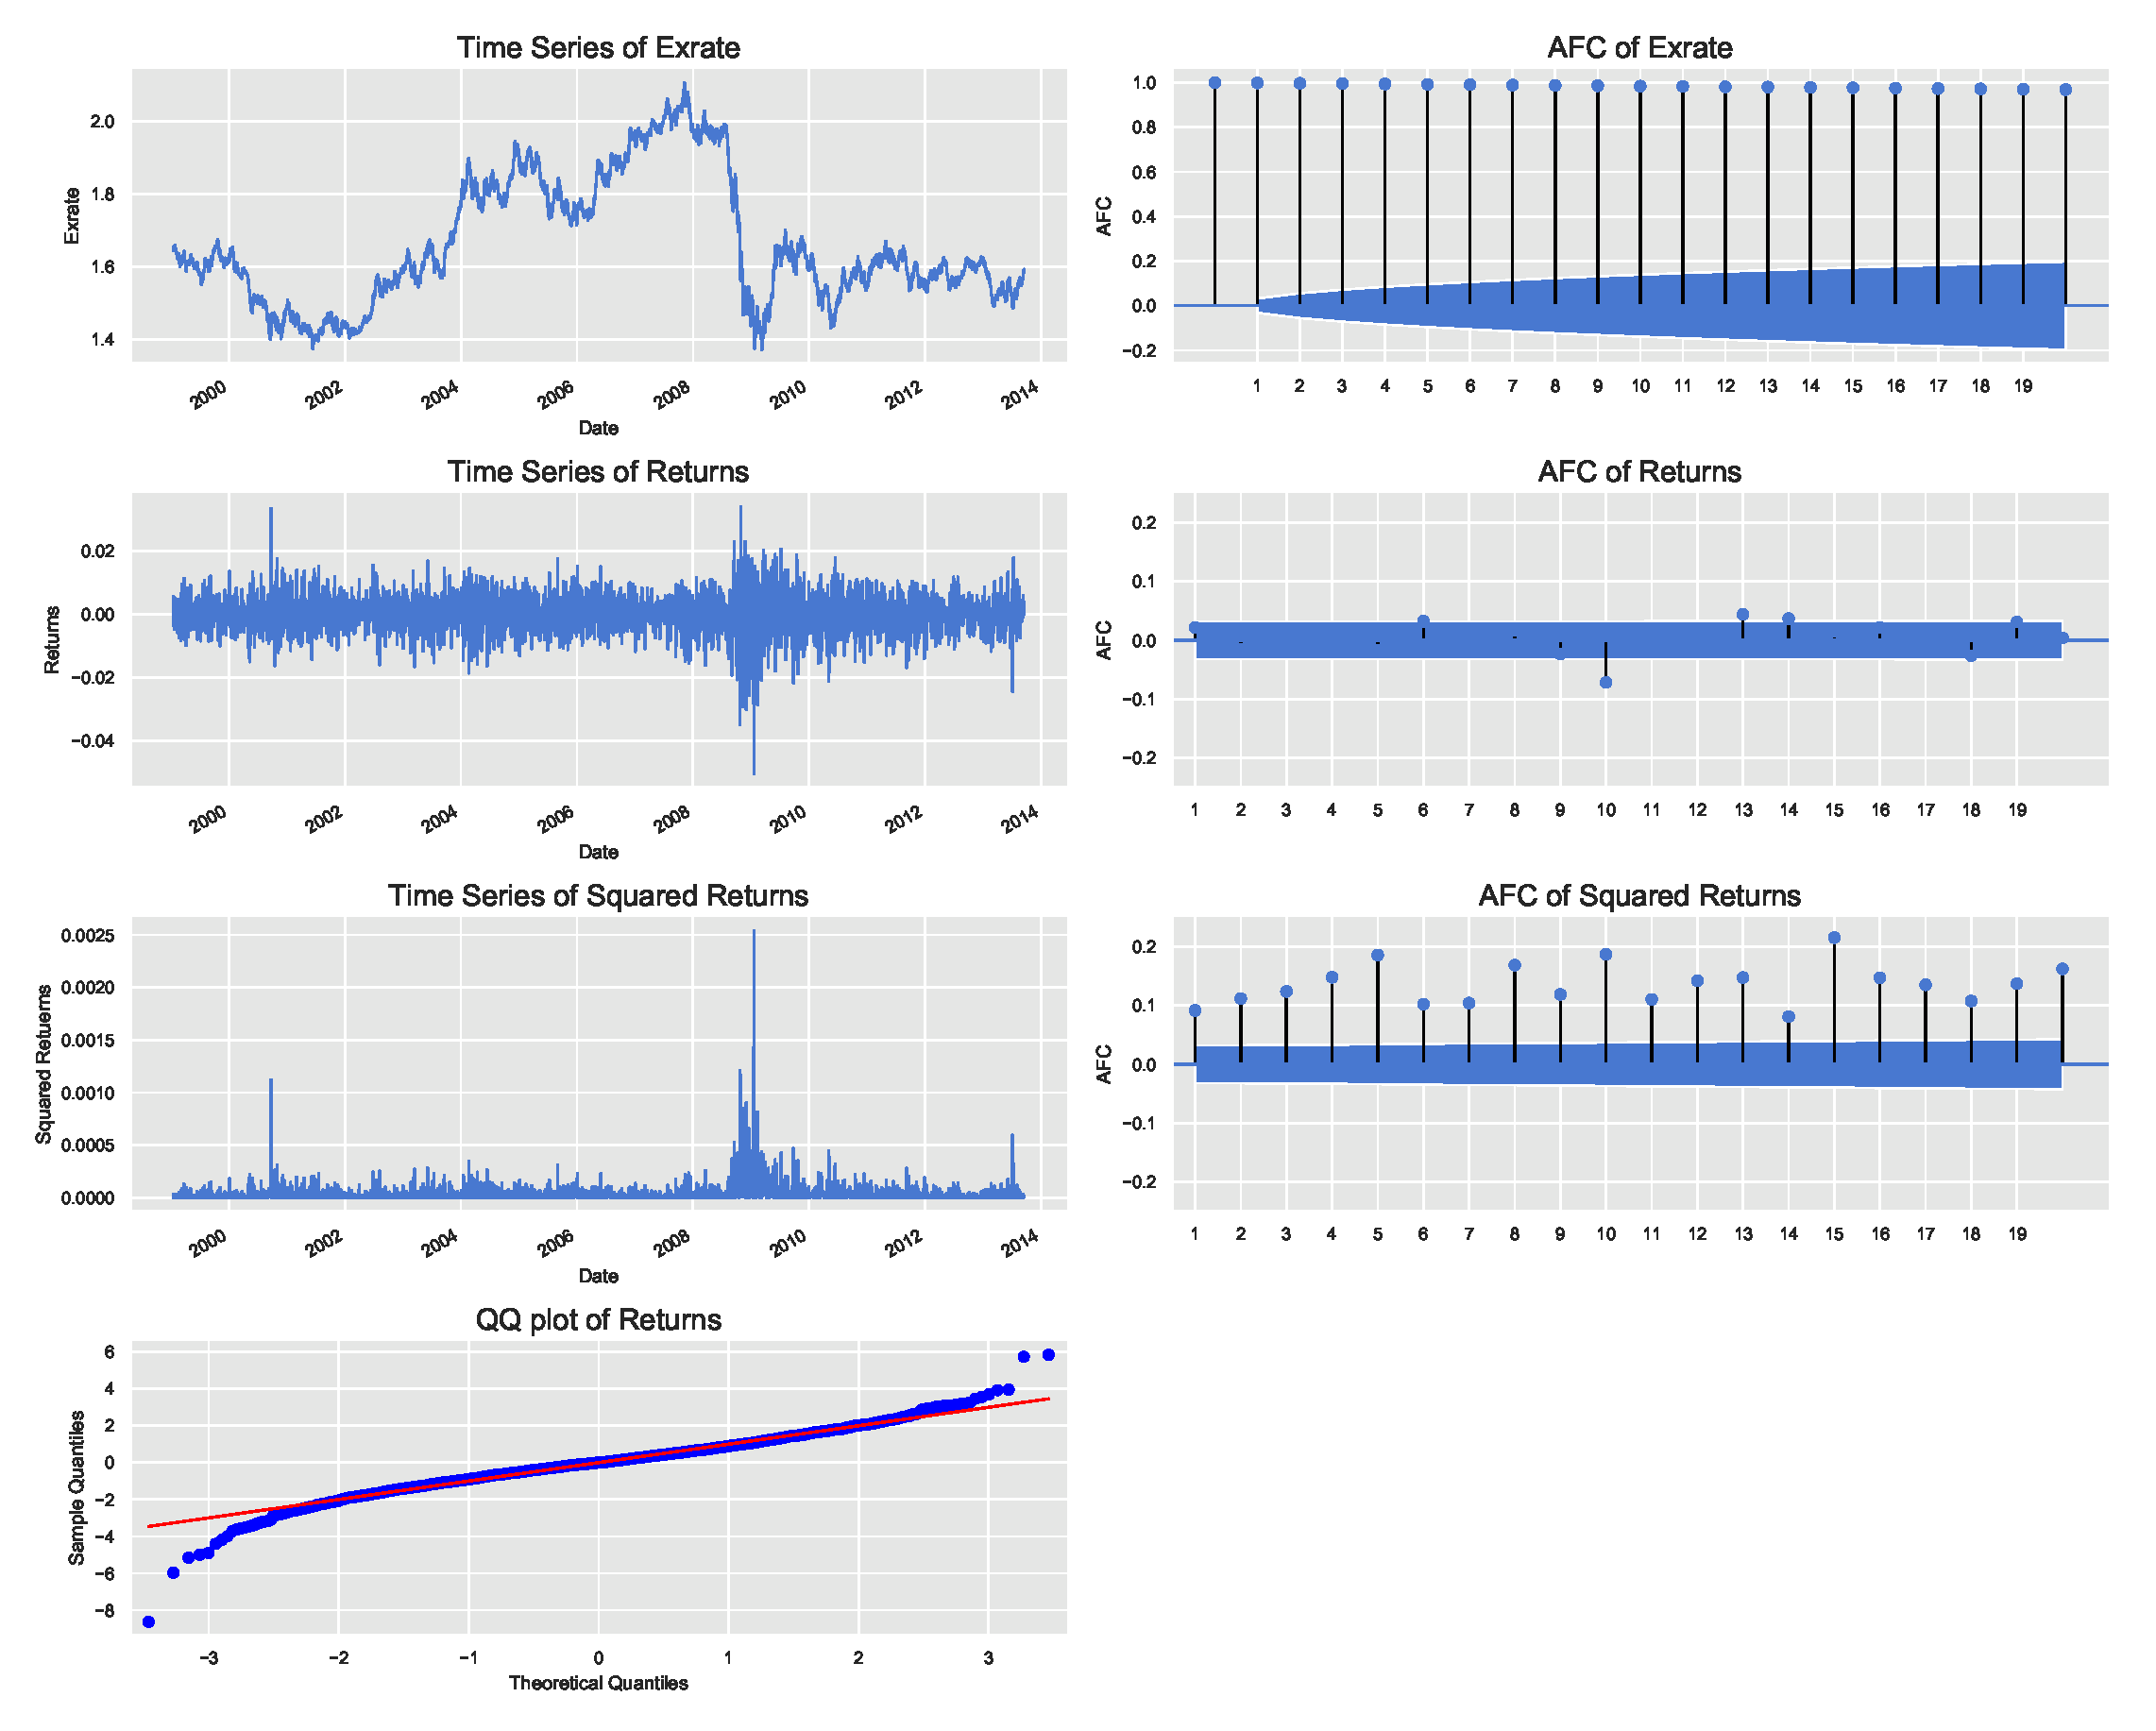
\includegraphics[width=\textwidth]{chapters/chapter_uvts/figures/31graphs.eps}
	\caption{Exchange rate related plots.\label{fig:exchrate}}
	\end{figure}

	\begin{figure}[!ht]
	\centering
	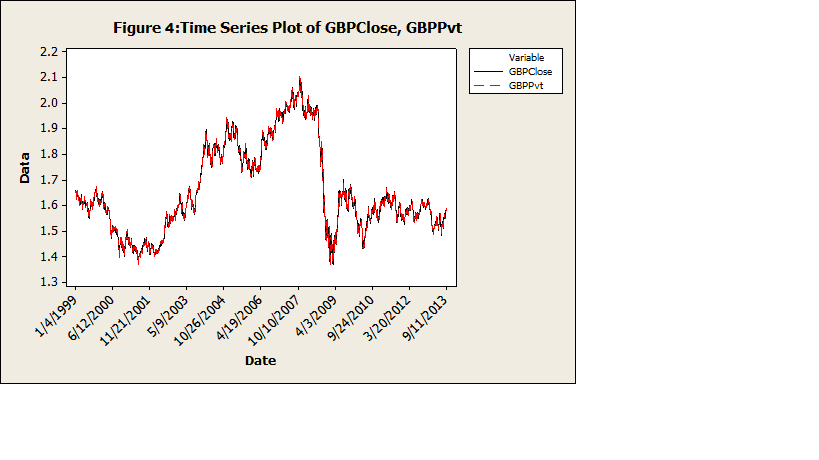
\includegraphics[width=\textwidth]{chapters/chapter_uvts/figures/Sec2-4Fig4.png}
	\caption{Times series plot of GBPClose, GBPPvt. \label{fig:timegbp}}
	\end{figure}
	
	\begin{figure}[!ht]
	\centering
	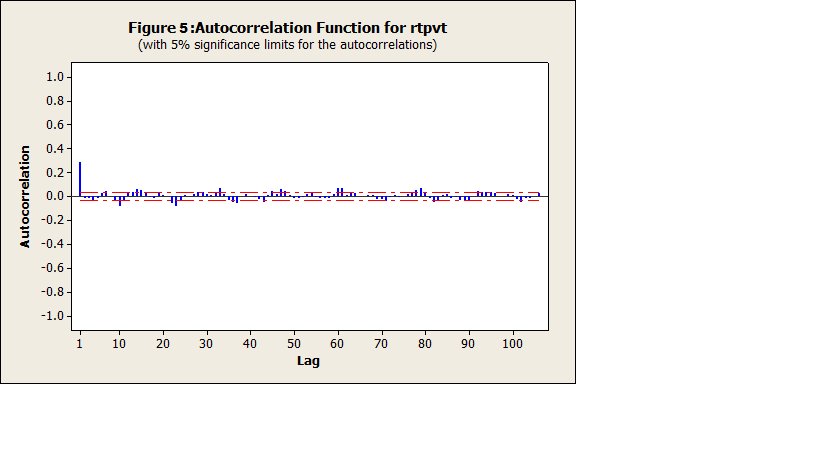
\includegraphics[width=\textwidth]{chapters/chapter_uvts/figures/Sec2-4Fig5.png}
	\caption{Autocorrelation function for rtpvt \label{fig:autocorrtpvt}}
	\end{figure}
An assumption of the random walk model that is often made is that the errors (returns)
follow a normal distribution. But in practice, the errors (or returns) tend to have heavier tails than the normal. We suggest using the quantile-quantile plot which is quite sensitive to even modest deviations from normality and also a test based on the properties of normal distribution. An omnibus test based on the skewness ($=0$ for normal) and the kurtosis ($=3$ for normal) is Jarque-Bera test:
	\begin{equation}\label{eqn:2JB}
	\text{JB }= n\left(\frac{\widehat{\text{SK}}^2}{6} + \frac{(\hat{K} - 3)^2}{24}\right) \sim \chi_2^2
	\end{equation}
where $\text{SK}\text{(ewness)}= E(\frac{X-\mu}{\sigma})^3, \text{K}\text{(urtosis)} = E(\frac{X-\mu}{\sigma})^4$. The corresponding sample numbers are substituted in JB (see Jarque and Bera (1980)\cite{jarque80}). The probability (Q--Q) plot of $r_t = \ln{(p_t)} - \ln{(p_{t-1})}$ as given in Figure 3 clearly indicates that the distribution has somewhat heavy tails. For this data $\widehat{SK} = -0.31$ and $\hat{K} = 3.67$ resulting in $\text{JB}= 129.7$ with $n= 3236$, thus rejecting the normal distribution. \\


\noindent\textbf{Stylized fact 2:} Heavy Tails: The returns are likely to display a heavy
tailed distribution such as a power-law or Pareto. \\


\noindent\textbf{Stylized fact 3:} Asymmetry: When prices fall, they tend to fall faster
than they tend to rise, thus drawdowns tend to be larger than upward rises. \\


These stylized facts are particularly important for risk management of strategies, and how they could be incorporated in trading decisions is still a subject of much research and will be discussed later.


\section{Time Series Models for Aggregated Data: Modeling the Variance}


In the ARMA$(p,q)$ model $\phi(B)Y_t= \delta + \theta(B) \,\varepsilon_t$ for series $\{Y_t\}$, when the errors $\varepsilon_t$ are \textit{independent} r.v.'s (with the usual assumptions of zero mean and constant variance $\sigma^2$), an implication is that the \textit{conditional} variance of $\varepsilon_t$ given the past information is a constant not depending on the past. This, in turn, implies the same feature for $l$-step ahead forecast errors $e_t(l) = \sum_{i=0}^{l-1}\psi_i\varepsilon_{t+l-i}$. However, in some settings, particularly for data from finance, the variability of errors may exhibit dependence on the past variability. Modeling the variance, which is essential for studying the risk-return relationship is an important topic in finance. \\


\noindent \textbf{Autoregressive Conditional Heteroscedastic (ARCH) Models} \\


The autoregressive conditional heteroscedastic (ARCH) models were originally proposed by Engle (1982)~\cite{engle1982}, Engle and Kraft (1983)~\cite{engle1983}, to allow for the conditional error variance in an ARMA process to depend on the past squared innovations, rather than be a constant as in ARMA models with independent errors. For example, an AR$(p)$ process with ARCH$(q)$ model errors is given as $Y_t = \sum_{i=1}^p\phi_iY_{t-i} + \delta + \varepsilon_t$, where,
	\begin{equation}\label{eqn:2ht}
	\begin{split}
	E&(\varepsilon_t\,|\,\varepsilon_{t-1},\varepsilon_{t-2},\cdots)= 0 \text{ and} \\
	h_t&= \Var(\varepsilon_t \,|\, \varepsilon_{t-1},\varepsilon_{t-2},\cdots) = E(\varepsilon_t^2\,|\,\varepsilon_{t-1},\varepsilon_{t-2},\ldots) = \omega_0 + \sum_{i=1}^q\omega_i\varepsilon_{t-i}^2
	\end{split}
	\end{equation}
with $\omega_0 > 0$ and $\omega_i \geq 0$ for $i= 1,\ldots,q$. In the generalized ARCH (GARCH) model, introduced by Bollerslev (1986)~\cite{bollerslev1986}, it is assumed that
	\begin{equation}\label{eqn:2secondht}
	h_t = E(\varepsilon_t^2|\varepsilon_{t-1},\varepsilon_{t-2},\cdots) = \omega_0 + \sum_{i=1}^q\omega_i\varepsilon_{t-i}^2 + \sum_{i=1}^k\beta_ih_{t-i},
	\end{equation}
where $\beta_i \geq 0$ for all $i = 1,\ldots,k$. Much subsequent research on and applications of the ARCH and GARCH models have occurred since the original research papers.


Let us briefly discuss some basic results and implications of the ARCH and GARCH models. The errors $\varepsilon_t$ in the model have zero mean, since $E(\varepsilon_t) = E[E(\varepsilon_t\,|\,\varepsilon_{t-1}\cdots)] = 0$, and they are serially uncorrelated; that is, $E(\varepsilon_t\varepsilon_{t-j}) = 0$ for $j \not= 0$ (since for $j > 0$, for example, $E(\varepsilon_t\varepsilon_{t-j}) = E[E(\varepsilon_t\varepsilon_{t-j}\,|\,\varepsilon_{t-1}\cdots)] = E[\varepsilon_{t-j}E(\varepsilon_t\,|\,\varepsilon_{t-1}\cdots)] = 0$). But the $\varepsilon_t$ are not mutually independent r.v.'s since they are inter-related through their conditional variances (i.e., their second moment). We will also assume that the $\varepsilon_t$ have equal unconditional variances, $\Var(\varepsilon_t) = \sigma^2$, for all $t$, so they are weakly stationary. Consider, then, the simple case of the first-order ARCH or ARCH(1) model,
	\begin{equation}\label{eqn:2htE}
	h_t = E(\varepsilon_t^2|\varepsilon_{t-1},\cdots) = \omega_0 + \omega_1\varepsilon_{t-1}^2,
	\end{equation}
Assuming that $\omega_1 < 1$ ($\omega_0$ and $\omega_1 \geq 0$ is always assumed), the \textit{unconditional} variance of $\varepsilon_t$ is $\sigma^2= \Var(\varepsilon_t) = \frac{\omega_0}{1 - \omega_1}$, since $\sigma^2 = E(\varepsilon_t^2) = E[E(\varepsilon_t^2|\varepsilon_{t-1},\cdots)] = E[\omega_0 + \omega_1\varepsilon_{t-1}^2] = \omega_0 + \omega_1\sigma^2$. Therefore, the conditional variance of $\varepsilon_t$ can be written as
	\begin{equation}\label{eqn:2htw}
	h_t = \omega_0 + \omega_1\varepsilon_{t-1}^2 = \sigma^2(1 - \omega_1) + \omega_1\varepsilon_{t-1}^2 = \sigma^2 + \omega_1(\varepsilon_{t-1}^2 - \sigma^2),
	\end{equation}
or in the form of deviation from the unconditional variance as $h_t - \sigma^2= \omega_1(\varepsilon_{t-1}^2 - \sigma^2)$. So the conditional variance will be above the unconditional variance whenever $\varepsilon_{t-1}^2$ exceeds its unconditional variance $\sigma^2$. If $\varepsilon_t$ were conditionally normally distributed, given the past, the fourth unconditional moment $E(\varepsilon_t^4)$ will exceed $3\sigma^4$ (the value in the normal distribution), so that the marginal distribution of $\varepsilon_t$ will exhibit fatter tails that the normal distribution. Conditional variances of multi-step ahead forecast errors can also be established to depend on the past squared errors. These basic results indicated for the ARCH(1) model also tend to hold for the higher order ARCH$(q)$ models. A basic impact of the ARCH errors in a process is in assessment of the accuracy of forecast, since the forecast errors will have conditional variances (given the past) that depend on the past. This allows for formation of correct and more informative (conditional) prediction intervals that would be obtained under the usual assumption that conditional error variances were constant independent of the past.


Now consider briefly the popular GARCH(1,1) model, $h_t = E(\varepsilon_t^2|\varepsilon_{t-1},\cdots) = \omega_0 + \omega_1\varepsilon_{t-1}^2 + \beta_1h_{t-1}$. Similar to the result for the ARCH(1) model, assuming that $\omega_1 + \beta_1 < 1$, it is readily shown that the unconditional variance of $\varepsilon_t$ is equal to $\sigma^2 = Var(\varepsilon_t) = \omega_0/[1 - (\omega_1 + \beta_1)]$. Let $v_t = \varepsilon_t^2 - h_t$, so that the r.v.'s $v_t$ have zero mean, and they are serially uncorrelated since
	\[
	\begin{split}
	E((\varepsilon_t^2 - h_t)(\varepsilon_{t-j}^2 - h_{t-j}))&= E[ E\{(\varepsilon_t^2 - h_t)(\varepsilon_{t-j}^2 - h_{t-j}) \,|\,\varepsilon_{t-1},\cdots\}] \\
	&= E[(\varepsilon_{t-j}^2 - h_{t-j}) E\{(\varepsilon_t^2 - h_t) \,|\,\varepsilon_{t-1},\cdots\}] = 0.
	\end{split}
	\]
Then, since $h_t = \varepsilon_t^2 - v_t$, note that the GARCH(1,1) model can be rearranged as $\varepsilon_t^2 - v_t = \omega_0 + \omega_1\varepsilon_{t-1}^2 + \beta_1(\varepsilon_{t-1}^2 - v_{t-1})$, or
	\begin{equation}\label{eqn:2ept}
	\varepsilon_t^2 = \omega_0 + (\omega_1 + \beta_1)\varepsilon_{t-1}^2 + v_t - \beta_1v_{t-1},
	\end{equation}
This form reveals that the process of squared errors, $\{\varepsilon_t^2\}$, follows an ARMA(1,1) model with uncorrelated innovations $v_t$ (however, the $v_t$ are conditionally heteroscedastic and more strongly are Martingale differences. Although this process looks like a linear process, it is not, since $ \{v_t\}$ are uncorrelated but dependent). This fact motivates the use of the ACF and PACF of the squares $\varepsilon_t^2$ for model specification and for basic preliminary checking for the presence of ARCH/GARCH effects in the errors $\varepsilon_t$. In practice, a starting point would be examination of the sample ACF and PACF of the squared residuals $\hat{\varepsilon}_t^2$, where $\hat{\varepsilon}_t$ are residuals obtained from fitting of a usual ARMA$(p,q)$ model (e.g., McLeod and Li, 1983~\cite{mcleod1983}). The correspondence between ARCH and ARMA is further noted via the condition, $0<\sum_{i=1}^q \omega_i<1$, that implies the roots of its characteristic equation lie outside the unit circle (like a causal ARMA).


For maximum likelihood (ML) estimation of models with ARCH or GARCH errors, assuming that $\varepsilon_t$ is conditionally normally distributed as $N(0,h_t)$, we have the log-likelihood function (apart from some initial conditions) given by $\log(L) = -\frac{T}{2} \log(2\pi) - \frac{1}{2}\sum_{t=1}^T \log(h_t) - \frac{1}{2}\sum_{t=1}^T \varepsilon_t^2/h_t$. Maximum likelihood estimation procedures, properties of the estimators, and Lagrange multiplier (LM) and likelihood ratio (LR) procedures for testing for the presence of ARCH effects in the conditional variances of the $\varepsilon_t$ have been considered by Engle (1982)~\cite{engle1982} and Weiss (1984) \cite{weiss1984}, among others.


As there are other excellent sources to learn about ARCH and GARCH models (see Tsay (2010)~\cite{tsay}, Chapter 3), we have limited our discussion to some basic details. \\


\noindent\textbf{Preliminary Testing for ARCH Effect:} The test is the omnibus test similar to Ljung-Box test that examines the presence of autocorrelation up to certain number of lags, which is equivalent to testing, $H_0: \alpha_1 = \alpha_2 \cdots = \alpha_q = 0$ in the model
	\begin{equation}\label{eqn:2eptsq}
	\varepsilon_t^2 = \alpha_0 + \alpha_1\varepsilon_{t-1}^2 + \cdots + \alpha_q\varepsilon_{t-q}^2 + a_t
	\end{equation}
where $a_t$ is white noise series; note that $\{a_t\}$ does not need to follow a normal distribution. The usual $F$-test used in regression can be applied here; Let $R^2$ be the coefficient of determination that result from (\ref{eqn:}) when $\hat{\varepsilon}_t$'s are used; then
	\begin{equation}\label{eqn:2F}
	F = \frac{R^2/q}{(1 - R^2)/(T - 2q - 1)} \sim \chi^2/q
	\end{equation}
We use $\chi^2$ instead of $F$ due to the fact that $\varepsilon_t$'s are estimated quantities. More informally, one could use the ACF of $\hat{\varepsilon}_t^2$ and if any of the autocorrelations are out of the normal bounds, $\pm 2/\sqrt{T}$, we may examine further for ARCH effects. \\


\noindent\textbf{GARCH vs ARCH:} While ARCH models care for the time dependence in volatilities and have elegant properties such as having excessive kurtosis (matching the empirical finding related to asset returns), they tend to overpredict the volatility and treat both negative and positive, $\varepsilon_t$'s symmetrically. To overcome some of these issues and as well as to come up with a more parsimonious representation (as in AR vs ARMA considerations) GARCH models stated in (\ref{eqn:2ept}) are proposed. \\


\noindent\textbf{IGARCH:} The variance can persist for extended periods and can change at different time spans, thus leading to non-stationary behavior. In the GARCH(1,1) model, it is possible that $w_1 + \beta_1 = 1$, so that IGARCH(1,1) (Integrated GARCH) can be written as
	\begin{equation}\label{eqn:2eptsqrt}
	\varepsilon_t = \sqrt{h_t} \cdot a_t,\qquad h_t = w_0 + w_1h_{t-1} + (1 - w_1)\varepsilon_{t-1}^2
	\end{equation}
If $h_t$ is proxied by $\varepsilon_t^2$, the above model leads to $\varepsilon_t^2 - \varepsilon_{t-1}^2 = w_0 + w_1(\varepsilon_{t-1}^2 - \varepsilon_{t-2}^2)$, which is similar in form to non-stationary autoregressive model. In practice because of level shifts in volatility, IGARCH appears to be a natural model to fit. Because the IGARCH(1,1) is similar to ARIMA(0,1,1), the model can be taken as an exponential smoothing model for the $\varepsilon_t^2$ series; By iterative substitutions, we can show that
	\begin{equation}\label{eqn:2ht1w}
	h_t = (1 - w_1)(\varepsilon_{t-1}^2 + w_1\varepsilon_{t-2}^2 + w_1^2\varepsilon_{t-3}^2 \cdots)
	\end{equation}
where $w_1$ can be taken as a discount factor. \\


\noindent\textbf{Prediction Performance of GARCH:} The predictive power of GARCH based on ex-post forecast evaluation criteria tend to suggest that the model provide poor forecasts, although the in-sample parameter estimates turn out to be highly significant. As Andersen and Bollerslev (1998)~\cite{andersen1998} note, in the model (\ref{eqn:2ept}), the latent volatility, $h_t$, evolves over time. The approach to evaluate the performance of the model for $h_t$ via $\hat{\varepsilon}_t^2$ is not appropriate. While $\hat{\varepsilon}_t^2$ provides an unbiased estimate of $h_t$, it is a noisy measurement due to idiosyncratic error terms associated with it; these error terms maybe due to the result of compounding frictions in the trading process. This will be clarified when we discuss the analysis of high-frequency data. \\


\noindent \textbf{Time--Varying ARCH Processes (tvARCH):} The underlying assumptions of ARCH models is stationarity and with changing pace of economic conditions the assumption of stationarity is not appropriate for modeling financial returns over long intervals. We may obtain a better fit by relaxing the assumption of stationarity. Dahlhaus and Subba Rao (2006)~\cite{dahlhaus2006} generalize the ARCH model with time-varying parameters:
	\begin{equation}\label{eqn:2eptsqrtht}
	\varepsilon_t = \sqrt{h_t}\cdot a_t,\quad h_t = w_0(t) + \sum_{j=1}^{\infty}w_j(t)\varepsilon_{t-j}^2
	\end{equation}
which $a_t$'s are i.i.d. with mean zero and variance, one. By rescaling the parameters to unit intervals, the tvARCH process can be approximated by a stationary ARCH process. A broad class of models resulting from (\ref{eqn:}) can be stated as:
	\begin{equation}\label{eqn:2eptN}
	\varepsilon_{t,N} = \sqrt{h_{t,N}}\cdot a_t,\quad h_{t,N} = w_0\left(\frac{t}{N}\right) + \sum_{j=1}^pw_j \left(\frac{t}{N}\right) \varepsilon_{t-j,N}^2
	\end{equation}
for $t= 1,2,\ldots,N$. This model captures the slow decay of the sample autocorrelations in squared returns that is commonly observed in financial data which is attributed to the long memory of the underlying process. But tvARCH$(p)$ is a non-stationary process that captures the property of long memory.


Fryzlewicz, Sapatinas and Subba Rao (2008)~\cite{fryzlewicz2008} propose a kernel normalized-least squares estimator which is easy to compute and is shown to have good performance properties. Rewriting (\ref{eqn:2eptN}) as
	\begin{equation}\label{eqn:2eptNsq}
	\varepsilon_{t,N}^2 = w_0\left(\frac{t}{N}\right) + \sum_{j=1}^p w_j\left(\frac{t}{N}\right)\varepsilon_{t-j,N}^2 + (a_t^2 - 1)h_{t,N}^2
	\end{equation}
in the autoregressive form, the least squares criterion with the weight function, $k(u_0,\chi_{k-1,N})$, where $\chi_{k-1,N}' = (1,\varepsilon_{k-1,N}^2,\ldots,\varepsilon_{k-p,N}^2)$ is
	\begin{equation}\label{eqn:2Lt0}
	L_{t_0,N}(\alpha) = \sum_{k=p+1}^N \frac{1}{b_N} \;w\left(\frac{t_0-k}{b_N}\right) \frac{\left(\varepsilon_{k\cdot N}^2 - \alpha_0 - \sum_{j=1}^p\alpha_j\varepsilon_{k-j\cdot N}^2\right)^2}{k(u_0, \chi_{k-1\cdot N})^2}
	\end{equation}
Minimizing (\ref{eqn:2Lt0}) yields, $\hat{a}_{t_0,N} = R_{t_0,N}^{-1}r_{t_0,N}$ where
	\begin{center}
	\begin{flalign}\label{eqn:2Rt0}
	&& R_{t_0,N}&= \sum_{k=p+1}^N \frac{1}{b_N}\ ; w\left(\frac{t_0-k}{b_N}\right) \frac{\chi_{k-1\cdot N}\chi_{k-1\cdot N}'}{k(u_0,\chi_{k-1\cdot N})^2} && \notag \\
	\text{and} && \phantom{x} & \phantom{x} && \\
	&& r_{t_0,N} &= \sum_{k=p+1}^N\frac{1}{b_N}\; w\left(\frac{t_0-k}{b_N}\right)\frac{\varepsilon_{k\cdot N}^2\chi_{k-1\cdot N}}{k(u_0,\chi_{k-1\cdot N})^2} && \notag
	\end{flalign}
	\end{center}
The kernel $w$ is a function defined on $[-\frac{1}{2},\frac{1}{2}]$ which is of bounded variation. The choice of weight function suggested is as follows: it is motivated by the differing variances at various values of $k$. Estimate,
	\begin{center}
	\begin{flalign}\label{eqn:2skN}
	&& \hat{\mu}_{t_0,N}&= \sum_{k=1}^N\frac{1}{b_N} \; w\left(\frac{t_0 - k}{b_N}\right)\varepsilon_{k\cdot N}^2 && \notag \\
	\text{and} && \phantom{x} & \phantom{x} && \\
	&& s_{k-1\cdot N} &= \sum_{j=1}^p\varepsilon_{k-j\cdot N}^2 && \notag
	\end{flalign}
	\end{center}
and use $k_{t_0,N}(s_{k-1},N) = \hat{\mu}_{t_0,N} + s_{k-1\cdot N}$ as the weight function. Thus the estimation is a two-stage scheme. For the bandwidth selection, the cross-validation method based on a subsample of the observations is suggested.


The methodology presented here is useful because of the changing nature of financial volatility. Real data applications will be discussed in Chapter 3.


\section{Stylized Models for Variance of Asset Returns}


Volatility has many important implications in finance. It is one of the most commonly
used risk measure and plays a vital role in asset allocation. The estimate of volatility of an asset is obtained using the prices of stock or options or both. Three different measures that are normally studied are stated below:
\begin{itemize}
\item Volatility is the conditional standard deviation of daily or low frequency returns.

\item Implied volatility is derived from options price under some assumed
relationship between the options and the underlying stock prices.

\item Realized volatility is an estimate of daily volatility using high frequency
intraday returns.
\end{itemize}
In this section we will mainly focus on the first item and the others will be discussed in a later section on high frequency data.


Consider $r_t = \ln{(p_t) - \ln{(p_{t-1})}}$, return of an asset. We observed that `$r_t$' exhibits no serial correlation. This does not imply that the series `$r_t$' consists of independent observations. The plot of $r_t^2$ given in Figure~\ref{fig:} clearly indicates that volatility tends to cluster over certain time spans. The autocorrelations in Figure~\ref{fig:} confirms that there is some time dependence for the volatility. In fact, there is some long range dependence that spans up to sixty days. \\


\noindent\textbf{Stylized fact 4:} Volatility clustering: High volatility events tend to cluster in time and this can be measured through positive correlations that exist over several lags.


To formally model the volatility, recall the conditional mean and the conditional variance of the return, $r_t$, are: $\mu_t = E(r_t \,|\,F_{t-1}),\sigma_T^2 = \Var(r_t\,|\,F_{t-1}) = E((r_t - \mu_t)^2\,|\,F_{t-1})$.


We have observed for the exchange rate series that $\mu_t \approx$ constant and is generally
close to zero. But $\sigma_t^2$ clusters around certain time spans and modeling variation
in $\sigma_t^2$ is typically done through ARCH/GARCH models and also through
stochastic volatility models. The stochastic volatility models have the advantage of modeling jumps in prices that are also often used in derivative pricing. To begin with, we can test for the heteroscedasticity using the test in (\ref{eqn:2F}) or one of the following which are all equivalent asymptotically:
\begin{itemize}
\item \textbf{Ljung-Box Omnibus Test:}
	\begin{equation}\label{eqn:2Qk}
	Q_k = T(T+2) \cdot \sum_{j=1}^k\frac{(\hat{e}^{j})^2}{T - j} \sim \chi_{k-m}^2
	\end{equation}
where $\hat{e}^{(j)}$ is the $j$th lag autocorrelation of $r_t^2$; $m$ is the number of independent parameters. Here $H_0: \rho_1 = \rho_2 = \cdots \rho_k = 0$.

\item \textbf{Lagrange Multiplier Test:} Regress $r_t^2$ on $r_{t-1}^2,\ldots,r_{t-q}^2$ and obtain $R^2$ the coefficient of determination; Test the $H_0$: Slope coefficients are all zero, by
	\begin{equation}\label{eqn:2TstarR}
	T \cdot R^2 \sim \chi_q^2
	\end{equation}
\end{itemize}
These tests were carried out on the exchange rate data; Table~\ref{tab:box} has the result of Ljung-Box Test: 
\begin{table}[!ht]
\centering
\caption{Ljung-Box Chi-Square Statistics for Exchange rate data \label{tab:box}}
	\begin{tabular}{ccccc}
	 h & 12 & 24 & 36 & 48 \\ \hline
	$Q_h$ & 73.2 & 225.7 & 463.4 & 575.7 \\ \hline
	df & 6 & 18 & 30 & 42 \\ \hline
	$p$-value & 0.000 & 0.000 & 0.000 & 0.000 \\
\end{tabular}
\end{table}


The Lagrange Multiplier test with $q=5$ also gives $R^2= 0.065$, that $T\cdot R^2= 243.6$ and compared with $\chi_5^2$ table values has $p$-value $\approx$ 0. These results clearly confirm that there is some time dependence in the volatility.


Among the conditional heteroscedasticity models ARCH/GARCH that were discussed in the last section, GARCH is simple to use and also results in more parsimonious modeling. Therefore, we present only the estimated GARCH model here. For exchange rate data, the estimated GARCH model is $\hat{\sigma}_t^2 = 2.61 \times 10^{-7} + 0.037r_{t-1}^2 + 0.95\hat{\sigma}_{t-1}^2$. Observe that the coefficients $r_{t-1}^2$ and $\hat{\sigma}_{t-1}^2$ add up to unity approximately and thus indicating the volatility is best modeled through IGARCH, which seems to hold generally for many asset volatilities.


\section{Other Topics: Bet Size etc.}






\section{Exercises (starred items have $R$-codes available)}


\begin{enumerate}[1.]
\item Consider the exchange rate daily data from December 4, 2006 to November 5, 2010 (Rupee versus Dollar, Pound and Euro), Rates.csv.
\begin{enumerate}[(a)]
\item Compute the sample average, standard deviation and the first order autocorrelation of daily returns over the entire sample period.  Test if the mean and the first order autocorrelation are significantly different from zero using the tests proposed in Section 2.3.2. 

\item Plot histograms of the returns over the entire sample period; Does the distribution look normal?  Test it through Jarque-Bera test in (\ref{eqn:?????}).

\item Aggregate the data at the weekly level; do (a) and (b) on the aggregated data. Compare the result with the result for the daily level.
\end{enumerate}

\item For the returns of all three time series in problem 1,  construct
\begin{enumerate}[(a)]
\item ARMA models for the returns; identify the model structure via ACF and PACF.

\item  GARCH models for the squared returns; compare the model coefficients for the three series.  Comment on the difference if any.

\item Is there a co-movement among the three exchange-rate series? To make the plots on a comparable scale, convert the starting points of the series unity. Does the co-movement vary over different time regimes? (Back up your claim with solid analysis.) Identify the transition states and speculate how you can exploit this for trading decisions. 
\end{enumerate}

\item Exchange Rates: The file \texttt{Exchange Rates.csv} contains exchange rates between US dollar and twenty-five major currencies. The daily data spans from Jan 3, 2000 to April 10, 2012. Use this data to perform the following tasks: after computing the returns, $r_t=\log(p_t)-\log(p_{t-1})$ for each series.

\begin{enumerate}[(a)]
\item Plot histograms of the returns and test if the distributions are normal, via Q--Q plots.

\item Compute the auto-correlation function and identify which lags are significant. What is the tentative ARMA model?

\item Is there any ARCH effect? Why?

\item Fit GARCH(1,1,) and IGARCH(1,1) models using both normal and t-distributions for the innovations. Which volatility model appears to be the best?
\end{enumerate}

 \item Exchange rates: Consider the original series, $p_t$, for the duration starting June 11, 2003.
 Answer the following after dividing each series by $p_1$, so that the starting points are the same.
\begin{enumerate}[(a)]
\item Identify for each series, if there are any regime changes. Test if these changes are statistically significant.

\item Identify how many clusters are there and if the membership changes under different regimes.

\item Are the series co-integrated? Use Johansen's rank test (\ref{eqn:}) to identify the number of co-integrating relationships. Interpret the coefficients of the co-integrating vectors.

\item Compare the results in (c)  with (b). What is the connection between clustering and co-integration? Briefly discuss.
\end{enumerate}


\item Consider daily price of Apple stock from Apple.cav. The data can be obtained from Yahoo Finance and have 7 columns (namely, Date, Open, High, Low, Close, Volume, Adj Close). We focus on the adjusted closing price in the last column. Note the data needs to be reversed from the past to the recent. 
\begin{enumerate}[(a)]
\item Compute the daily log returns. Is there any serial correlation in the daily log returns? Use the test for white noise as outlined in the text. 

\item Consider the pivot quantities on the average of high and low price and the average of high, low and close prices. Compute the returns based on the pivot log prices and test for serial correlation. Compare this result with the finding in (a). 

\item Consider the log price series of AAPL stock. Is the log price series unit-root nonstationary? Perform a unit-root (Dickey-Fuller) test to answer the question and present your conclusion.
\end{enumerate}

\item Consider daily price of Apple stock again.
\begin{enumerate}[(a)]
\item Compute various measures of variance computed from the entries of the price bars. Comment on their correlation with log volume. 

\item Use the ARIMA modeling to come up with a parsimonions model for log volume. Comment on the model accuracy by setting aside a validation data set. 
\end{enumerate}


\item The \textit{Roll} model for trade prices discussed in the text can be more specifically stated as,
	\[
	\begin{split}
	p_t^*&= p_{t-1} + \epsilon_t, \;\;\;\;\; \epsilon_t \sim N(0,\sigma^2) \\
	\text{and } p_t&= p_t^* + c s_t, \;\;\;\;\; \text{where }s_t \in \{+1,-1\}
	\end{split}
	\]
Here $p_t^*$ is the ``true'' value of a security and $p_t$ is the observed trade price, which differ because of the bid-offer spread: $c$ is the half-spread and $s_t$ is the direction of the $t$th trade. $s_t$ and $\epsilon$ are serially independent and independent of each other.
\begin{enumerate}[(a)]
\item Calculate the serial correlation of the observed prices $p_t$. Construct an MA(1) model with the same autocorrelation structure. Of the two such models, take the invertible one. 

\item For the invertible model, construct the associated AR model. 

\item Use the model to show how to estimate the bid-ask spread and apply the results on the Apple data used in Problem (5) and (6). \\
\end{enumerate}


\textbf{Questions 8--10 refer to Level III data descried below:} \\


The dataset consists of (CSV) file that contains the entire trading session, including early and late hours from 6:00~a.m. to 8:00~p.m. EST. It contains intraday depth book activity several major tickers from up to 5 major national exchanges: Nasdaq, Direct Edge, NYSE, ARCA, and BATS (exact number of exchanges depends on the historical period). All messages are consolidates into one file ordered by timestamp. This dataset allows to build a full national depth book (super book) at any moment intraday. 

\begin{table}[h!]
   \caption{Column Format}
   \centering
   \begin{tabular}{p{2cm}p{8cm}} 
   \textbf{Column} & \text{Description} \\ \hline
   Timestamp & Number of milliseconds after the midnight. \\ \hline
   Ticker & Equity symbol (up to 8 characters) \\ \hline
   Order & Unique order ID. \\ \hline
   T & Message type. Allowed Values: \newline
	~~\llap{\textbullet}~~ ``B''--Add buy order \newline
	~~\llap{\textbullet}~~ ``S''--Add sell order \newline
	~~\llap{\textbullet}~~ ``E''--Execute outstanding order in part \newline
	~~\llap{\textbullet}~~ ``F''--Execute outstanding order in full \newline
	~~\llap{\textbullet}~~ ``D''--Delete outstanding order in full \newline 
	~~\llap{\textbullet}~~ ``X''--Bulk volume for the cross event \newline
	~~\llap{\textbullet}~~ ``T''--Execute non-displayed order  \\ \hline
   Shares & Order quantity, available for the ``B'', ``S'', ``E'', ``X'', ``C'', ``T'' messages. Zero for ``F'' and ``D'' messages. \\ \hline
   Price & Order price, available for the ``B'', ``S'', ``X'', and ``T'' order messages. Zero for cancellation and executions. The last 4 digits are decimal digits. The decimal portion is padded on the right with zeros. The decimal point is implied by position; it does not appear inside the price field. Divide by 10000 to convert into currency value. \\ \hline
   MPID & Market Participant ID associated with the transaction (4 characters) \\ \hline
   MCID &U Market Center Code (originating exchange--1 character)
   \end{tabular}
\end{table}


For the analysis of Problems 8--10, we consider the data for CISCO.

 
\item You need to aggregate the data into 5-min intervals before answering the following.
\begin{enumerate}[(a)]
\item Let $x_t$ denote the number of trades in the $t$th 5-minute interval. Ignore the time gaps between trading days. Plot the time series and its ACF. Determine if there are intraday period patterns in the series.

\item Using the last transaction in the $t$th 5-minute interval as the stock price in that interval, plot the
time series $y_t$ of 5-minute returns during the period and the corresponding ACF.

\item Consider the bivariate time series ($x_t$, $y_t$). How does $y_t$ vary with $x_t$? Are there intraday periodic patterns in ($x_t$, $y_t$)?

\item Plot the durations of the transaction times for Mondays and Fridays. Is there any difference in the
patterns?

\item Fit GARCH models for the durations and interpret the coefficients.

\item Is there any particular exchange that offers better price?
\end{enumerate}



\item Use the transaction data in Problem 8. There are seventy-eight five-minute intervals in a trading day. Let $d_i$ be the average of all log durations for the $i$th 5-minute interval across all trading days. Let $t_j$ be tick time of a trade during the $i$th 5-minute interval, define an adjusted duration as $\Delta t_j^* = \Delta t_j/\exp(d_i)$ where $\Delta t_j = t_j - t_{j-1}$.
\begin{enumerate}[(a)]
\item Is there a diurnal pattern in the adjusted duration series?

\item Build EACD and WACD models for the adjusted duration and compare them. Now aggregate the data over the 5-minute intervals; Let $r_t$ be the return and $V_t$ is the volume of transactions in the $t$th interval.

\item Is there any relationship between the volume $V_t$ and volatility $r_t^2$ . If there is develop a model that will capture the dependence of volatility on volume. Let $\overline{p}_t$ be the average price in the $t$th 5-minute
interval.
\end{enumerate}


\item Use the CISCO execution data only; aggregate at various time intervals: 1~min, 2~min, \dots, 15~min. For these levels record
\begin{enumerate}[(a)]
\item Average price, VWAP, realized volatility and aggregate volume.

\item By relating the returns and volatility estimates based on average price to realized volatility, identify the optimal duration for aggregation that will cancel out the market friction but pick up the true information. (You may want to refer to Bandi and Russell (2006)~\cite{bandi}). 
\end{enumerate}




\end{enumerate}




% !TEX root = ../../book.tex

\chapter{Multivariate Time Series Models}

\section{Blah Blah}
TO DO


% !TEX root = ../../book.tex

\chapter{Advanced Topics}


In this chapter we want to discuss some advanced methods that are applicable in the context of trading. This chapter is broadly divided into two main areas; the first covers topics which are extensions of models discussed in Chapter 2 in the low frequency context. Although the state-space modeling is discussed in the context of ARIMA, its scope is much wider. We also outline the established methodology for studying regime switching, but indicate the areas of further research where predicting ahead using signals form the past when the regime shift is likely to occur. This is followed by a discussion on using volume information to study the price volatility. With the increased exploitation of price behavior data, it has become necessary to look for additional signals. The second area of this chapter focuses on the models from point processes to study the higher frequency data. Here our approach has been to provide an intuitive discussion of main tools; as readers will realize, the trade data is quite noisy and there is a great deal of scope to do research especially in non-parametric modeling of arrivals and cancellations in the limit order market. 


\section{State-Space Modeling} 


There has been much recent interest in the representation of ARIMA models in the state-space form, for purpose of forecasting, as well as for model specification and maximum likelihood estimation of parameters. This approach helps to update the model coefficients as and when new data arrives. 


The state-space models were initially developed by control systems engineers to measure a signal contaminated by noise. The signal at time ``$t$'' is taken to be a linear combination of variables, called state variables that form the so called state vector at time, $t$. The key property of the state vector is that it contains the minimum set of information from past and present data but the future behavior of the system is independent of the past value and depends only on the present values. Thus the state vector evolves according to the Markov property. The state equation is stated as,
	\begin{equation}\label{eqn:2zt}
	Z_t = \Phi_tZ_{t-1} + a_t
	\end{equation}
and observation equation
	\begin{equation}\label{eqn:2yt}
	Y_t = H_tZ_t + N_t
	\end{equation}
where it is assumed that $a_t$ and $N_t$ are independent white-noise processes; $a_t$ is a vector white noise with covariance matrix $\Sigma_a$ and $N_t$ has variance $\sigma_N^2$. The matrix $\Phi_t$ in (\ref{eqn:2zt}) is an $r \times r$ transition matrix and $H_t$ in (\ref{eqn:2yt}) is a $l \times r$ vector, which are allowed to vary in time.


We will consider the state-space form of an ARIMA$(p,d,q)$ process $\phi(B)Y_t = \theta(B)\,\varepsilon_t$, define the forecasts $\hat{Y}_t(j) = E(Y_{i+j}\,|\,Y_t,Y_{t-1},...)$ for $j= 0,1,\ldots,r$, with $r= \max(p+d,q+1)$, and $\hat{Y}_t(0) = Y_t$.


From the updating equations $\hat{Y}_{t+1}(l) = \hat{Y}_t(l+1) + \psi_l\varepsilon_{t+1}= \hat{Y}_t(l + 1) + \psi_l\, [Y_{t+1} - \hat{Y}_t(1)]$ for the general ARIMA model, we have that $\hat{Y}_t(j - 1)= \hat{Y}_{t-1}(j) + \psi_{j-1}\varepsilon_t$, $j = 1,2,\ldots,r-1$. Also for $j= r>q$, observe that $\hat{Y}_t(j-1)= \hat{Y}_{t-1}(j) + \psi_{j-1}\varepsilon_t = \sum_{i=1}^{p+d}\phi_i\hat{Y}_{t-1}(j - i) + \psi_{j-1}\varepsilon_t$. So we define the ``state'' vector at time $t$, $Z_t$, with $r$ components as $Z_t = (Y_t, \hat{Y}_t(1),\cdots,\hat{Y}_t(r-1))'$. Then from the above relations we find that $Z_t$ satisfies the equations
	\[ 
	Z_t = \begin{bmatrix}
                        0 & 1 & 0 & \cdots & 0 \\
                        0 & 0 & 1 & \cdots &  0 \\
                        \vdots & \vdots &\ddots  &  &  \vdots \\
                        0 & 0 &  & \ddots &  1 \\
                        \phi_r & \phi_{r-1} & \cdots & \cdots &  \phi_1
                    \end{bmatrix}
                    \,Z_{t-1} + 
                    \begin{bmatrix}
                    1\\ \vdots \\ \vdots \\ \psi_{r-1}
                    \end{bmatrix}
                    \,\varepsilon_t
                    \]
where $\phi_i = 0$ if $i > p + d$. So we have
	\begin{equation}\label{eqn:2secondzt}
	Z_t = \Phi Z_{t-1} + \Psi\varepsilon_t
	\end{equation}
together with the observation equation
	\begin{equation}\label{eqn:2thirdzt}
	Z_t = Y_t + N_t = [1,0,\ldots,0] \,Z_t + N_t = H Z_t + N_t
	\end{equation}
where the additional noise $N_t$ would be present only if the ARIMA process $\{Y_t\}$ is observed subject to additional noise; otherwise we simply have $Z_t \equiv Y_t = HZ_t$. The above two equations constitute what is known as a state-space representation of the ARIMA model. We note that there are many other constructions of the state vector $Z_t$ that will give rise to state-space equations of the general form of (\ref{eqn:2zt})--(\ref{eqn:2yt}); that is, the state-space form of an ARIMA model is not unique.

Observe, in applications the matrices $\Phi_t$ and $H_t$ are constant matrices, $\Phi \equiv \Phi_t$ and $H \equiv H_t$ for all $t$, that do not depend on $t$, as in the state-space form (\ref{eqn:2secondzt})--(\ref{eqn:2thirdzt}) of the ARIMA model. In this case the system or model is said to be time-invariant. A nice feature of expressing a model in state-space form is that an updating procedure can be readily used when a new observation becomes available to revise the current state vector and to produce forecasts. These forecasts in general tend to fare better. 

For the state-space model, define the finite sample estimates of the state vector $Z_{t+1}$ based on observations $Y_t,\cdots,Y_l$ over the finite past time period, as
	\[
	\hat{Z}_{t+l|t} = E[Z_{t+l}|Y_t,\cdots,Y_l],\text{ with } V_{t+l|t} = E[(Z_{t+l} - \hat{Z}_{t+l|t})(Z_{t+l} - \hat{Z}_{t+l|t})'].
	\]
A convenient computational procedure, known as the \textit{Kalman filter equations}, is then available to obtain the current estimate $\hat{Z}_{t|t}$, in particular. It is known that, starting from some appropriate initial values $Z_0 \equiv \hat{Z}_{0|0}$ and $V_0 \equiv V_{0|0}$, the optimal filtered estimate, $\hat{Z}_{t|t}$, is given through the following recursive relations:
	\begin{equation}\label{eqn:2hatz}
	\hat{Z}_{t|t} = \hat{Z}_{t|t-1} + K_t(Y_t - H_t\hat{Z}_{t|t-1})
	\end{equation}
where $K_t= V_{t|t-1} H_t'[H_t V_{t|t-1} H_t' + \sigma_N^2]^{-1}$ with $\hat{Z}_{t|t-1} = \Phi_t \hat{Z}_{t-1|t-1},V_{t|t-1} = \Phi_t V_{t-1|t-1} \Phi_t' + \Sigma_{a}$ and $V_{t|t} = [I - K_tH_t] V_{t|t-1} = V_{t|t-1} - V_{t|t-1} H_t' [H_t V_{t|t-1} H_t' + \sigma_N^2]^{-1} H_t V_{t|t-1}$ for $t=1,2,\cdots$.


In (\ref{eqn:2yt}), the quantity $\varepsilon_{t|t-1}= Y_t - H_t \hat{Z}_{t|t-1} \equiv Y_t - \hat{Y}_{t|t-1}$ is called the (finite sample) innovation at time $t$, because it is the new information provided by the measurement $Y_t$ which was not available from the previous observed (finite) history of the system. The factor $K_t$ is called the ``Kalman gain'' matrix. The filtering procedure in (\ref{eqn:2hatz}) has the recursive ``prediction-correction'' or ``updating'' form, and the validity of these equations as representing the minimum mean square error predictor can readily be verified through the principles of ``updating''. For example, verification of (\ref{eqn:2hatz}) follows from the principle, for linear prediction, that
	\[
	\begin{split}
	E[Z_t\,|\,Y_t,\ldots,Y_1]&= E[Z_t|Y_t - \hat{Y}_{t|t-1},Y_{t-1},\cdots,Y_1] \\
	&= E[Z_t\,|\,Y_{t-1},\cdots,Y_1] + E[Z_t \,|\, Y_t - \hat{Y}_{t|t-1}],
	\end{split}
	\]
since $\varepsilon_{t|t-1} = Y_t - \hat{Y}_{t|t-1}$ is independent of $Y_{t-1},\ldots,Y_1$. From (\ref{eqn:2hatz}) it is seen that the estimate of $Z_t$ based on observations through time $t$ equals the prediction of $Z_t$ from observations through time $t-1$ updated by the factor $K_t$ times the innovation $\varepsilon_{t|t-1}$. The quantity $K_t$ can be interpreted as the regression coefficients of $Z_t$ on the innovation $\varepsilon_{t|t-1}$, with $\Var(\varepsilon_{t|t-1}) = H_t V_{t|t-1} H_t' + \sigma_N^2$ and $\Cov(Z_t,\varepsilon_{t|t-1})= V_{t|t-1}H_t'$ following directly from (\ref{eqn:2thirdzt}) since $\varepsilon_{t|t-1} = H_t (Z_t - \hat{Z}_{t|t-1}) + N_t$. Thus, the general \textit{updating relation} is $\hat{Z}_{t|t} = \hat{Z}_{t|t-1} + \Cov(Z_t,\varepsilon_{t|t-1})\{\Var(\varepsilon_{t|t-1})\}^{-1}\varepsilon_{t|t-1}$, where $\varepsilon_{t|t-1} = Y_t - \hat{Y}_{t|t-1}$, and the relation in $V_t$ is the usual updating of the error covariance matrix to account for the new information available from the innovation $\varepsilon_{t|t-1}$, while the \textit{prediction relations} (\ref{eqn:2hatz}) follow directly from (\ref{eqn:2secondzt}). In general, forecasts of future state values are available directly as $\hat{Z}_{t+l|t} = \Phi_{t+l} \hat{Z}_{t+l-1|t}$ for $l = 1,2,\ldots$ with the covariance matrix of the forecast errors generated recursively essentially through (\ref{eqn:2pteq}) as $V_{t+l|t} = \Phi_{t+l}V_{t+l-1|t} \Phi_{t+l}' + \Sigma_a$. Finally, forecasts of future observations $Y_{t+l}$ are then available as $\hat{Y}_{t+l|t} = H_{t+l} \hat{Z}_{t+l|t}$, since $Y_{t+l|t} = H_{t+l} Z_{t+l} + N_{t+l}$, with forecast error variance $v_{t+l|t} = E[(Y_{t+l} - \hat{Y}_{t+l|t})^2] = H_{t+l}V_{t+l|t}H_{t+l}' + \sigma_N^2$.


For ARIMA models, with state-space representation (\ref{eqn:2secondzt})--(\ref{eqn:2thirdzt}) and $Y_t = HZ_t$ with $H = [1,0,\ldots,0]$, this Kalman filtering procedure constitutes an alternate method to obtain exact finite sample forecasts, based on data $Y_t,Y_{t-1},\cdots,Y_1$, for future values in the ARIMA process, subject to specification of appropriate initial conditions to use in the terms in (\ref{eqn:2hatz}). For stationary zero-mean processes $Y_t$, the appropriate initial values are $\hat{Z}_{0|0} = 0$, a vector of zeros, and $V_{0|0} = \Cov(Z_0) \equiv V_*$, the covariance matrix of $Z_0$ which can easily be determined under stationarity through the definition of $Z_t$. Specifically, since the state vector $Z_t$ then follows the stationary vector AR(1) model $Z_t = \Phi Z_{t-1} + \psi\varepsilon_t$, its covariance matrix $V_*= \Cov(Z_t)$ satisfies $V_*= \Phi V_*\Phi' + \sigma_{\varepsilon}^2\Psi\Psi'$, which can be readily solved for $V_*$. For nonstationary ARIMA processes, additional assumptions need to be specified. The ``steady-state'' values of the Kalman filtering procedure $l$-step ahead forecasts $\hat{Y}_{t+l|t}$ and their forecast error variances $v_{t+l|t}$, which are rapidly approached as $t$ increases, will be identical to the expressions given previously, $\hat{Y}_t(l)$ and $\sigma^2(l) = \sigma^2(1 + \sum_{i=1}^{i-1}\psi_{i}^2)$


In particular, for the ARIMA process in state-space form, we can obtain the exact (finite sample) one-step ahead forecasts $\hat{Y}_{t-1}(1) = E[Y_t\,|\,Y_{t-1},\ldots,Y_1] = H \hat{Z}_{t|t-1}$, and their error variances $v_{t|t-1} = H V_{t|t-1} H'$, conveniently through the Kalman filtering equation (\ref{eqn:2hatz}). This can be particularly useful for evaluation of the Gaussian likelihood function, based on $T$ observations $Y_1,\cdots,Y_T$ from the ARIMA process, applied to the problem of maximum likelihood estimation of model parameters.

This state-space approach to exact likelihood function determination has also been shown to be quite useful in dealing with estimation problems for ARMA models when some values $Y_t$ of the series are not observed, that is, there are missing values among the sequence of $Y_t$ values.

An alternative set-up, alternative to (\ref{eqn:2thirdzt}) and (\ref{eqn:2hatz}) is to assume that the deviations in the observation and transition equations are related. With the observation equation stated in (\ref{eqn:2yt}), the transition equation is modified as 
	\begin{equation}\label{eqn:223zt}
	Z_t = \Phi Z_{t-1} + \alpha N_t 
	\end{equation}
This model studied in Ord, Koehler, and Snyder (1997)~\cite{ord1997estimation} with a single source of error $(N_t)$ is shown to be closely related to various exponential smoothing procedures. There are other formulations of state-space models, such as structural models by Harvey (1989)~\cite{harvey1989kalman} and dynamic linear models of West and Harrison (1997)~\cite{west1997} that are found to be useful for model building.


\section{Regime Switching and Change-Point Models}


It has been long noted in finance that there are two kinds of recurrences in stock prices: underreaction and overreaction to a series of good or bad news. The securities that have a good record for an extended period tend to become overpriced and have low returns subsequently. Barberis, Shleifer and Vishny (1998)~\cite{vishny} present a model where investor believes that the returns can arise from one of two regimes although returns follow random walk: mean-reverting or trending. The transition probabilities are taken to be fixed and the regime is more likely to stay the same rather than to switch. But the investor's beliefs are updated as and when the returns data are observed. It is presumed that in many instances, we may not discern these shifts directly whether or when they occur but instead can draw probabilistic inference based on the observed behavior posthumously. Hamilton (2016)~\cite{jdham} reviews models for regime-switching applied in several contexts in macroeconomics, building upon the elegant model introduced in Hamilton (1989)~\cite{89ham}. Here in this section, we will cover only studies that are relevant to finance applications, particularly relevant to trading that exploit anomalies. 


Consider the model,
	\begin{equation}\label{eqn:modelham}
	y_t = \mu_{s_t} + \epsilon_t, \quad s_t=1,2
	\end{equation} 
where $y_t$ is the observed variable, such as asset return and $s_t$ represents two distinct regimes and $\epsilon_t$'s are i.i.d.$\sim N(0,\sigma^2)$. Let $\{F_{t-1}\}$ be the information set available as of `$t-1$'. The transition between the regimes is taken to be Markovian,
	\begin{equation}\label{eqn:markprob}
	\text{Prob}(s_t=j \;|\; s_{t-1}=i, F_{t-1})= p_{ij}, \quad i,j=1,2
	\end{equation}
thus leading to an AR(1) model for $\mu_{s_t}$ as
	\begin{equation}\label{eqn:must}
	\mu_{s_t} = \phi_0 + \phi_1 \mu_{s_{t-1}} + a_t
	\end{equation}
where $a_t$ by definition can take four possible values depending upon $s_t$ and $s_{t-1}$. Here $\phi_0=p_{21}\mu_1 + p_{12} \mu_2$ and $\phi_1=p_{11}-p_{21}$. Note the model for $y_t$ in (\ref{eqn:modelham}) is the sum of an AR(1) process and white noise, then from Theorem~\ref{thm:agg}, $y_t \sim$ ARMA(1,1); but because of discrete nature of `$a_t$', (\ref{eqn:modelham}) is a non-linear process. Note that the unknown parameters are $(\mu_1,\mu_2,\sigma,p_{11},p_{22})'=\lambda$ and they can be estimated via maximum likelihood as follows: note $y_t|(s_t=j,F_{t-1})\sim N(\mu_j,\sigma^2)$. The predictive density of $y_t$ is given as,
	\begin{equation}\label{eqn:predden}
	f(y_t \;|\; F_{t-1})= \sum_{i=1}^2 \text{Prob}(s_t=i \;|\; F_{t-1}) \, f(y_t \;|\; s_t=i, F_{t-1})
	\end{equation}
and estimate of $\lambda$ is obtained by maximizing the likelihood function $L(\lambda)=\sum_{t=1}^T \log f(y_t \;|\; F_{t-1}, \lambda)$. Two useful quantities are: \\


\noindent Predicted regime: 
	\begin{equation}\label{eqn:predreg}
	\text{Prob}(s_t=j \;|\; F_{t-1})= p_{1j} \text{Prob}(s_{t-1}=1 \;|\; F_{t-1}) + p_{2j} \,\text{Prob}(s_{t-1}=2 \;|\; F_{t-1})
	\end{equation}
\noindent Optimal forecast:
	\begin{equation}\label{eqn:optfore}
	E(y_t \;|\; F_{t-1})= \sum_{i=1}^2 (\phi_0+\phi_1 \mu_i) \text{Prob}(s_{t-1}=i \;|\; F_{t-1}).
	\end{equation}
The forecast for `$k$' period ahead can be stated as:
	\begin{equation}\label{eqn:period}
	E(y_{t+k} \;|\; F_{t-1}) = \mu+\phi_1^k \sum_{i=1}^2 (\mu_i-\mu)\, \text{Prob}(s_t=i \;|\; F_{t-1})
	\end{equation}
where $\mu=\phi_0/(1-\phi_1)$.


The basic model has been extended to cover multiple regimes and to vector processes. Interested readers should refer to Hamilton (2016)~\cite{jdham} and references therein. Ang and Timmermann (2012)~\cite{timmerman} discuss a model that accounts for changes not only in the mean but also in variances and autocorrelations:
	\begin{equation}\label{eqn:varautoy}
	y_t= \mu_{s_t} + \phi_{s_t} y_{t-1} + \epsilon_t
	\end{equation}
where $\epsilon_t$'s are independent $\sim N(0,\sigma_{s_t}^2)$. Using the data on excess S\&P500 returns, FX returns, etc., it is identified that there are volatility regimes, but no level shifts.


Hamilton (1990)~\cite{90ham} proposes using EM (Expectation-Maximization) algorithm (Dempster, Laird and Rubin (1977)~\cite{dempster}) to obtain the maximum likelihood estimate, instead of recursive filter approach (see Hamilton (1989)~\cite{89ham} to optimize the loglihood of (\ref{eqn:predden}), updated with $y_t$. Note by Bayes' Theorem
	\begin{equation}\label{eqn:bayes}
	\text{Prob}(s_t=j \;|\; F_t) = \dfrac{\text{Prob}(s_t=j \;|\; F_{t-1}) \, f(y_t\;|\; s_t=j, F_{t-1})}{f(y_t \;|\; F_{t-1})}
	\end{equation}
To get an estimate of $p_{ij}$ in step `$l+1$', use 
	\begin{equation}\label{eqn:hatpijl}
	\hat{p}_{ij}^{(l+1)}= \dfrac{\sum_{t=1}^{T-1} \text{Prob}(s_t=i, s_{t+1}=j \;|\; F_t, \hat{\lambda}^{(l)})}{\sum_{t=1}^{T-1} \text{Prob}(s_t=i \;|\; F_t, \hat{\lambda}^{(l)})}
	\end{equation}
and with these estimates obtain the ML estimates of the rest of the parameters ($\mu_1$, $\mu_2$, and $\sigma$) by maximizing the likelihood function. More details can be found in Hamilton (1990)~\cite{90ham}.


There is a vast literature on Bayesian approach to this problem, see for example, Chib (1998)~\cite{chib} and subsequent publications that followed. An interesting application is given in Pastor and Stambaugh (2001)~\cite{pastor}. Lai and Xing (2013)~\cite{laixing} study a general model, somewhat similar to (\ref{eqn:varautoy}):
	\begin{equation}\label{eqn:arxgarch}
	\text{ARX-GARCH:} \quad y_t= \beta_t' x_t + v_t \sqrt{h_t} \, \epsilon_t
	\end{equation}
where $h_t\sim$ GARCH$(p,q)$ and $\beta_t$ and $v_t$ are piecewise linear. Using the weakly returns of S\&P500 index, AR(1)-GARCH(1,1) model is attempted and it is identified that 1998--2003 had higher volatility. Figure~\ref{fig:sp500} provides the plot of closing price, returns, volatility and volume data. 


	\begin{figure}[!ht]
	\centering
	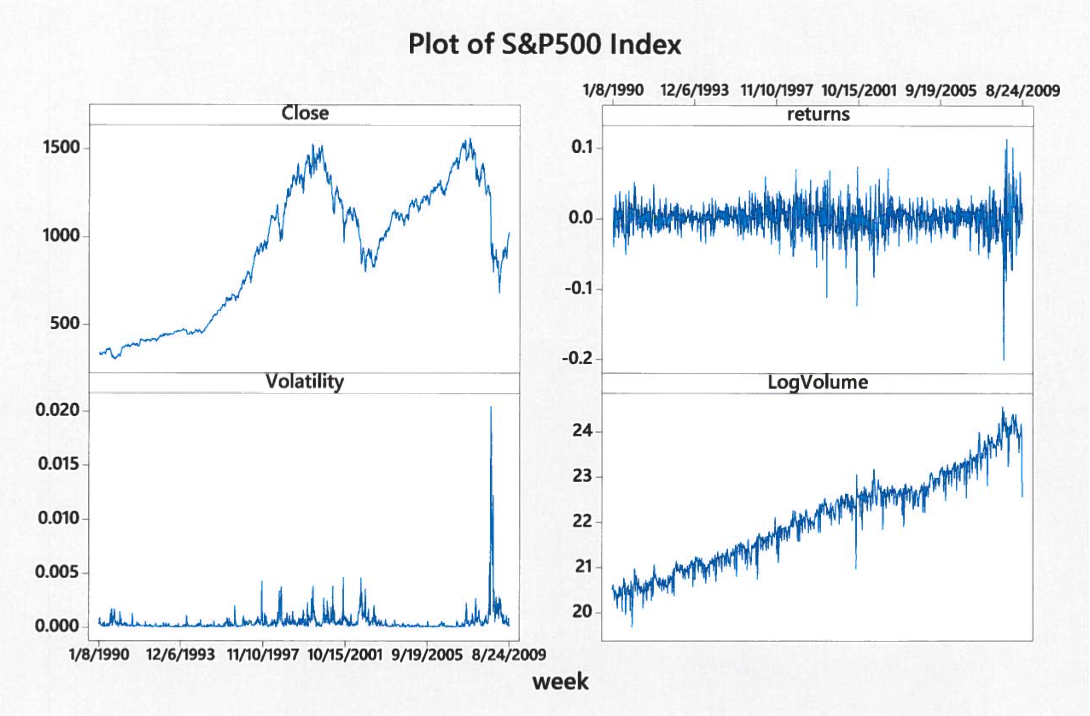
\includegraphics[width=\textwidth]{chapters/chapter_uvts/figures/sp500.png}
	\caption{Plot of S\&P 500 Index. \label{fig:sp500}}
	\end{figure}


In most of the applications of the above regime-switching models, particularly in finance, the plots of relevant quantities clearly reveal the pattern and these models provide a way to confirm the level and size shifts. We want to conclude this section with some simple ideas borrowed from the area of statistical process control. Recall that if the market is efficient, the return $r_t=\ln P_t - \ln P_{t-1}\sim $ IID $(\mu_t, \sigma^2)$, but $\mu_t=\delta$ when $t\geq t_0$ and zero elsewhere. The cumulative sum chart (CUSUM) to detect the positive and negative mean shift are based on recursive calculations:
	\begin{equation}\label{eqn:cdouble}
	\begin{split}
	c_t^+&=\max(0,c_{t-1}^+ + (r_t-k)) \\
	c_t^-&=\min(0,c_{t-1}^- - (r_t-k))
	\end{split}
	\end{equation}
where $k=\delta/2$. The chart signals as sown as $c_t^+$ reaches `$h$'---a decision point set by the user. Jiang, Shu and Apley (2008)~\cite{shuap} modify (\ref{eqn:cdouble}) with exponentially weighted moving average (EWMA) type of estimates that is adaptive in nature. It can be stated as,
	\begin{equation}\label{eqn:elma}
	s_t^+=\max\left(0,s_{t-1}^+ + w(\hat{\delta}_t)\left(r_t - \frac{\hat{\delta}_t}{2}\right)\right)
	\end{equation}
where $w(\hat{\delta}_t)$ is a weight function; a simple weight function $w(\hat{\delta}_t)=\hat{\delta}_t$ is suggested. The $\delta_t$ is updated as 
	\begin{equation}\label{eqn:updatedelt}
	\hat{\delta}_t=(1-\lambda)\, \hat{\delta}_{t-1} + \lambda r_t
	\end{equation}
The adaptive CUSUM chart is effective at detecting a range of mean shift sizes. Similar results for the variance need to be worked out.


In practical applications of these regime-shifting models, it is not easy to discern between a single outlier and persistent level shift. Valid measures that can distinguish these two situations on a timely basis could be very valuable to a trader. 


We provide two examples to illustrate the application of the models (\ref{eqn:2secondzt}) and (\ref{eqn:2thirdzt}) in the broader context of this book. The slope in a local linear trend is a random walk. Specifically,
	\begin{equation}\label{eqn:randomwalk}
	\begin{split}
	p_t&= \mu_t+ e_t \\
	\mu_t&= \mu_{t-1} + \delta_{t-1} + \eta_{0t} \\
	\delta_t&=\delta_{t-1}+\eta_{1t}
	\end{split}
	\end{equation}
Here the trend is composed of level `$\mu_t$' and slope `$\delta_t$'. The slope `$\delta_t$' when written as 
	\begin{equation}\label{eqn:slopewritten}
	\delta_t= D+ e(\delta_{t-1} - D)+ \eta_{1t}
	\end{equation}
in AR(1) form is sometimes known as generalized local linear trend. These models can be written in the form of (\ref{eqn:2secondzt}) and (\ref{eqn:2thirdzt}); the updating process given in (\ref{eqn:2hatz}) can be used to accommodate a wide range of models.


Menkveld, Koopman and Lucas (2007)~\cite{menkkoop} study the price discovery process for stocks that are cross-listed in two different markets via state-space models. The question if the trading location matters more than business location is of intent to finance researchers. Consider a stock traded in Amsterdam and in NY exchanges. Because of the time difference, there is only an hour of overlap in trading. Ignoring this aspect, write the two-dimensional price vector as
	\begin{equation}
	\begin{split}
	p_t&=\mu_t + e_T \\
	&=\mu_t + \theta(\mu_t-\mu_{t-1}) + e_t
	\end{split}
	\end{equation}
as the observational equation and the state equation is
	\begin{equation}
	\mu_t= \mu_{t-1} + \xi_t
	\end{equation}
The above can be written in the form of (\ref{eqn:2secondzt}) and (\ref{eqn:2thirdzt}) with appropriate choice of `$\Phi$' and `$H$' matrices. 


\section{A Model for Volume-Volatility Relationship}


While the price information via returns and the volatility can be modeled through methods described earlier, it has become important to incorporate other relevant trading data to augment the trading strategies. To that effect, we want to seek some guidance from economic theory how that information is linked to price movements.

In the market microstructure theory, it is assumed that price movements occur primarily due to the arrival of new information and this information is incorporated efficiently into market price. Other variables such as trading volume, bid-ask spread and market liquidity are observed to be related to the volatility of the returns. Early empirical studies have documented a positive relationship between daily trading volume and volatility (See Clark (1973)~\cite{clark}). Epps and Epps (1976)~\cite{epps} and Tauchen and Pitts (1983)~\cite{tauchenpitts} assume that the volume and price are driven by the underlying `latent' information ($I$) and provide a theoretical framework to incorporate this information. Assuming that there are fixed number of traders who trade in a day and the number of daily equilibria, $I$ is random because the number of new pieces of information is random, the return and the volume are written as a bivariate normal mixture model with the same mixing variable $I$. Conditional on $I$:
	\begin{equation}\label{eqn:2rtVt}
	\begin{split}
	 r_t&= \sigma_1\sqrt{I_t}Z_{1t} \\
	 V_t&= \mu_VI_t + \sigma_2\sqrt{I_t}Z_{2t}
	 \end{split}
	 \end{equation}
where $Z_{1t}$ and $Z_{2t}$ are standard normal variables and $Z_{1t}, Z_{2t}$, and $I_t$ are mutually independent. Thus the volatility-volume relationship,
	\begin{equation}\label{eqn:2covVt}
	\begin{split}
	\Cov(r_t^2,V_t)& = E(r_{t}^2V_t) - E(r_t^2) \,E(V_t) \\ 
	&= \sigma_1^2\mu_V \Var(I_t) > 0
	\end{split}
	\end{equation}
is positive due to the variance in $I_t$. If there is no new information or if there is no variation in the mixing variable, $\Var(I_t)= 0$ and thus the relationship vanishes. The theory of arrival rates suggest a
Poisson distribution and based on empirical evidence, the lognormal distribution is taken to be a candidate for distribution of mixing variable, $I_t$. The parameters of the model in (\ref{eqn:2rtVt}) are estimated through maximum likelihood. Gallant, Rossi and Tauchen (1992)~\cite{grt} using a semi-parametric estimate of the joint density of $r_t$ and $V_t$ conduct a comprehensive study of NYSE data from 1925 to 1987. The following summarizes their findings: \\


\noindent\textbf{Stylized Facts 5 (Volume--Volatility Relationship):} 

\begin{itemize}
\item  Positive correlation between conditional volatility and volume.

\item Large price movements are followed by high volume.

\item Conditioning on lagged volume substantially attenuates the leverage (which is an asymmetry in the conditional variance of current price change against past price change) effect.

\item After conditioning on lagged value, there is a positive risk-return relation.
\end{itemize}


Andersen (1996)~\cite{andersen} modifies the model (\ref{eqn:2rtVt}) by integrating the microstructure
setting of Glosten and Milgrom (1985)~\cite{glostenmilgrom} with the stochastic volatility, that is built on weaker conditions on the information arrival process. While the first equation in (\ref{eqn:2rtVt}) remains the same, the volume $V_t$ has informed and noise components, $V_t = IV_t + NV_t$. Noise trading component, $NV_t$ is taken as a time homogeneous Poisson process, $P_0(m_0)$. Therefore, the systematic variation in trading is mainly due to informed volume. Then $IV_t|I_t \sim \text{Poisson}(I_t\mu)$ and thus
	\begin{equation}\label{eqn:2VtIt}
	V_t|I_t \sim \text{Poisson}(m_0 + I_t m_1)
	\end{equation}
It is easy to see $\Cov(r_t^2,V_t) = \sigma^2m_1 \Var(I_t) > 0$ under this setting as well. These models clearly indicate that the intraday return volatility and volume processes jointly contain predictable elements.


There are other studies that focus on the trading volume and returns relationship and we mention only a select few here. Campbell, Grossman, and Wang (1993)~\cite{campbellgross} demonstrate for individual large stocks and stock indices the first-order daily auto-correlation in the returns tend to decline with volume. The authors develop a theoretical model where the economy has two assets, risk-free asset and a stock and there are two types of investors, one with constant risk aversion and the other with risk aversion changing over time. Under this set-up, it is implied that a decline in a stock price on a high-volume day is more likely than a decline on a low-volume day to be associated with an increase in the expected stock return.


Gervais, Kaniel, and Mingelgrin (2001)~\cite{gervais2001high} investigate the role of trading activity in providing information about future prices. It is shown that periods of extremely high (low) volume tend to be followed by positive (negative) excess returns. The formation period for identifying extreme trading volume is a day or a week, but the effect lasts at least twenty days and holds across all stock sizes. To test if this information can be used profitably, the authors construct a trading strategy, by sending buy (sell) limit orders at the existing bid (ask) price, at the end of the formation period. If the orders are not taken, they are converted into market orders at the closing. The strategy is shown to result in profits, in particular with the small-medium firm stocks, after adjusting for the transaction costs. The model used for the empirical framework is the vector autoregressive model discussed later, with an addition of a set of exogenous control variables:
	\begin{equation}\label{eqn:2Ytphi}
Y_t = \Phi_0+\sum_{j=1}^p\Phi_jY_{t-j}+\sum_{l=1}^LB_lX_{t-l}+\epsilon_t
	\end{equation}


The components of $Y_t$ include stock or market related variables such as detrended log of stock turnover, the stock return and the value weighted market return. The control variables are market volatility based on the daily return standard deviation and the dispersion which is the cross-sectional standard deviation of the security returns. The impulse response functions are used to aggregate the overall relationship among the endogenous variables. Statman, Thorley, and Vorkink (2006)~\cite{statman2006investor} show that the trading volume is dependent on past returns over many months and it is argued that this may be due to the overconfidence of the investors.


These and other studies generally confirm the information content of the volume and turnover of stocks traded; strategies to exploit these, especially in a high frequency context, will be examined in Chapter 3. We will discuss how intra-day flow of volume can be related to price changes. 


In algorithmic trading a key ingredient of many strategies is forecast of intra-day volume. Typically a parent order is split into several child orders and the timing of the submission of child orders could depend on the volume forecast for an interval of time that is considered for trading. Brownless, Cipollini and Gallo (2011)~\cite{brownless} provide prediction model for intra-day volume. This will be described in detail in the next chapter.


\section{Models for Point Processes}


In many fields of study, observations occur in a continuum, space or time in the form of point events. The continuum can be multi-dimensional, but our focus is on the one-dimensional time scale with points distributed irregularly along the time scale. The main interest lies in estimating the mean rate of occurrence of events or more broadly on the patterns of occurrence. There are excellent monographs on this topic: Cox and Lewis (1966) \cite{cox1966}, Daley and Vere-Jones (2003)~\cite{daley2003}, etc. But the interest in financial applications was revived by the seminal paper by Engle and Russell (1998)~\cite{engle1998}. Financial market microstructure theories as discussed in Kyle (1985) \cite{kyle1985}, Admati and Pfleiderer (1988)~\cite{admati1988theory} and Easley and O' Hara (1992)~\cite{easley1992} suggest that the frequency and the timing of transactions, that include posting, canceling and executing an order, carry information about the state of the market. The transactions generally tend to cluster during certain times of the day and the change in the mean rate of occurrences may suggest a new information flow about a stock.


To illustrate, recall Figure~\ref{fig:}, on trading activities in Section 2.1. If we denote the observed intervals between successive activities as durations by $d_1, d_2,\ldots,d_r$, the time of occurrences are obtained by forming the cumulative sums of the $d$'s, $t_1=d_1, t_2=t_1+d_2, \ldots, t_r=t_{r-1}+d_r$. Cox and Lewis (1966)~\cite{cox1966} suggest two ways to present this type of data graphically. One method is based on cumulative numbers of events that have occurred at or before `$t$' against `$t$'. The slope of the line between any two points is the average number of events per unit for that period. One way to standardize the plot would be to approximate the graph by a line, `$at$' when `$a$' is the slope of the graph indicating the average rate of occurrence for the entire duration. The second method calls for dividing the time scale into equally spaced time intervals and count the number of events in each interval; this also can be modified by fixing a certain number of events and spacing on the time it takes for this number to occur. In the context of stock price data, this could mean simply recording not when the trade occurs but when the price changes. The advantage of the second plot is that the local fluctuations are readily observed and the advantage of the first plot is that it enables us to see systematic changes in the rate of occurrence.
 
 	\begin{figure}[!ht]
	\centering	
	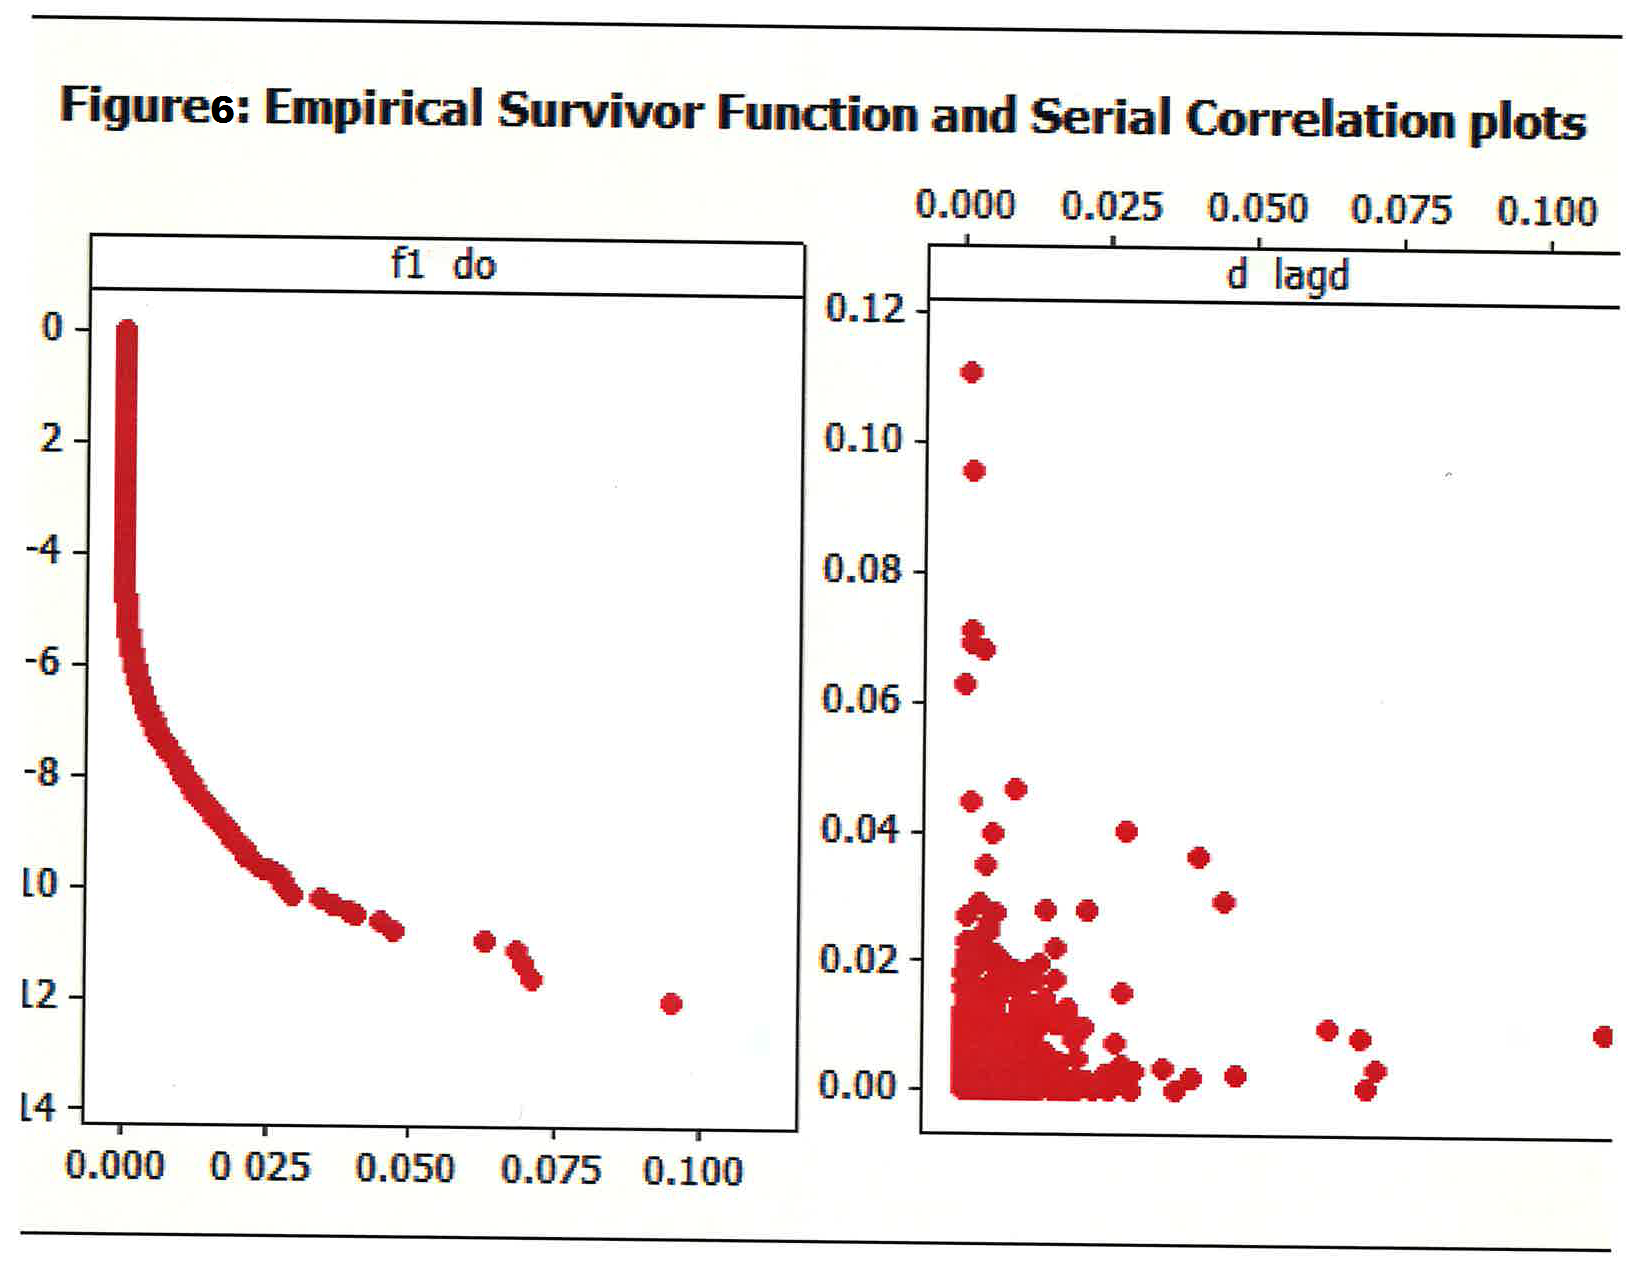
\includegraphics[width=\textwidth]{chapters/chapter_uvts/figures/Sec2-10Fig6.png}
	\caption{Empirical Survivor Function and Serial Correlation plots. \label{fig:survivor}}
	\end{figure}
	
	\begin{figure}[!ht]
	\centering
	 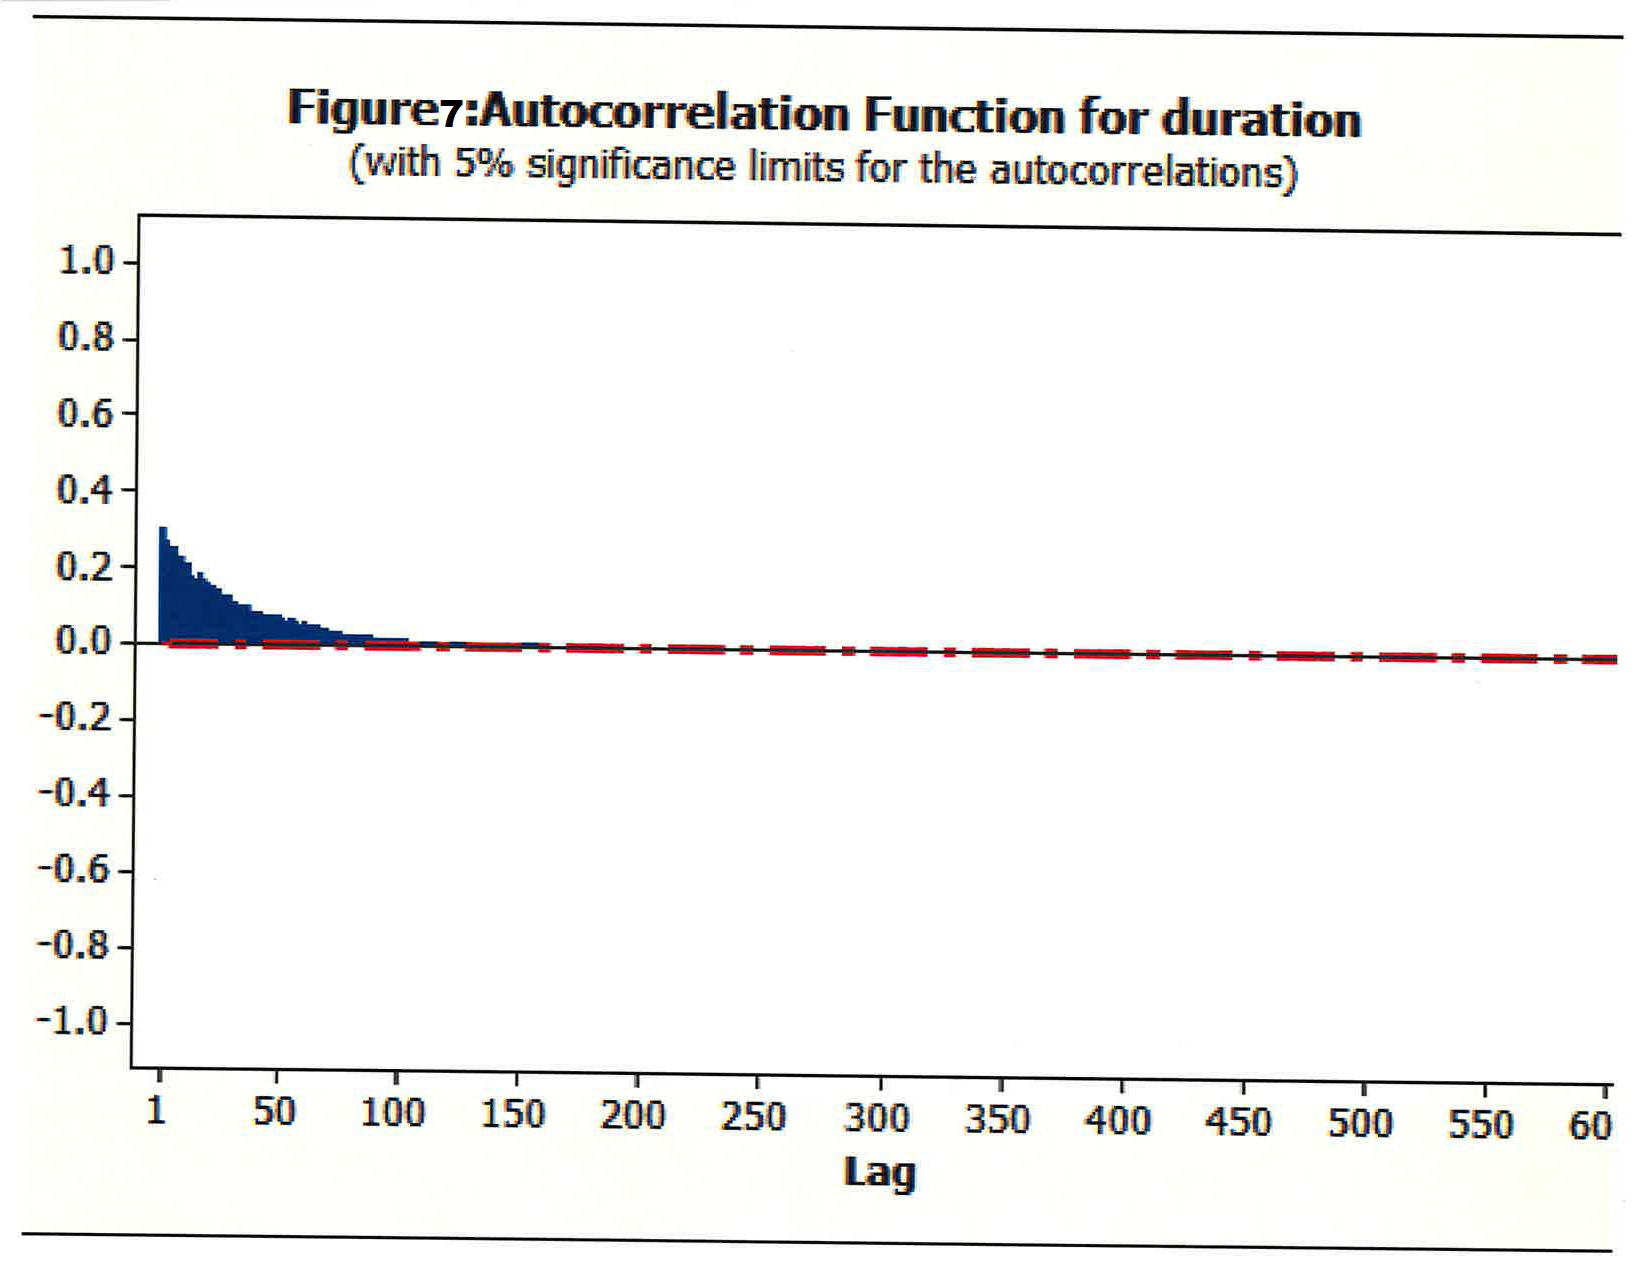
\includegraphics[width=\textwidth]{chapters/chapter_uvts/figures/Sec2-10Fig7.png}
	\caption{Autocorrelation Function for duration. \label{fig:duration}}
	\end{figure}
 
 The baseline distribution for the durations is exponential resulting from Poisson arrivals for a specified interval that assume a constant rate. It is suggested to plot log(1-$\frac{i}{n_0+1})$ against $d_{(i)}$ where $d_{(i)}$ results from the ordered durations, $d_{(1)} \leq d_{(2)} \leq ... \leq d_{(n_0)}$ calculated between successive $n_0+1$ occurrences. Departures from linearity would indicate that the exponential distribution may not hold. In addition it is also suggested to plot $d_{i+1}$ against $d_i$ to check on the dependance of durations. Cox and Lewis (1966, p14)~\cite{cox1966} state that, ``It is not clear how correlation in such data should be measured and tested; in particular it is not obvious that the ordinary correlation coefficient will be the most suitable measure with such data''. Engle and Russell (1998)~\cite{engle1998} show how the dependence in the duration data can be explicitly modeled in the context of high frequency transaction data. We illustrate this with the trading data for Microsoft (MSFT) for the month of January in the year 2013. This graph (Figure~\ref{fig:survivor}) clearly indicates that the durations do not follow an exponential distribution and do exhibit some dependence. This is confirmed by the autocorrelation function for durations (Figure~\ref{fig:duration}).


Cox and Lewis (1966)~\cite{cox1966} also observe a few issues that can arise with the point-process type data. It is possible that two or more events recorded as happening at the same time. This may be due to latency issues but if they occur due to genuine coincidences it is better to analyze the number of events attached to each occurrence time as a variate separately. Further complications are that there may be events, such as price and volume that may be interdependent and events that occur with related series that may be useful for modeling and predicting the future occurrence times.


\subsection{Stylized Models for High Frequency Financial Data}


There has been a great deal of interest in studying market micro-structure to better understand the trading mechanisms and the process of price formation. With the availability of Trades and Quotes (TAQ) data that contains all equity transactions on major exchanges, it has now became possible to better understand the market micro-structure. The extensive details from the order books over multiple exchanges have provided massive amount of data. Analyzing these data will be taken up in later chapters as well. Here we want to present some unique characteristics of the high frequency data and present most commonly used models in practice. To reiterate, the transactions (trades, quotes, bids, etc) may occur at any point in time (Figure~\ref{fig:exchhours}) during the exchange hours as given below.
	\begin{figure}[!ht]
	\centering
	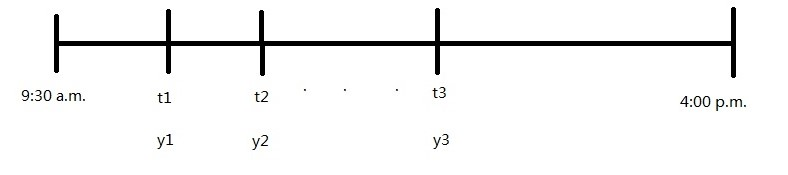
\includegraphics[width=\textwidth]{chapters/chapter_uvts/figures/33d1.jpg}
	\caption{Exchange hours. \label{fig:exchhours}}
	\end{figure}
High-frequency data refer to the `tick' `$t_i$' data which contains, in addition to the exact time of even occurrence, `$y_i$' called marks that may refer to all other elements of the limit order book such as traded price or quote etc. The traditional time series methods that we discussed in the context of low frequency data analysis are not applicable here as the ticks can occur at any point in time when the exchange are open. Standard econometric techniques are for data in discrete time intervals. Aggregating the high-frequency data to some fixed time interval will not capture the advantages of having access to detailed transaction data. Even for some heavily traded stocks, if the intervals are chosen to be short, there may be many intervals with no data and if the intervals are long, the microstructure features will be lost. Also certain key features such as the imbalance between bid side and ask side of the limit order book and when and how the market orders cross the spread are not easy to aggregate in a fixed time interval, however short or long it may be. Moreover, the timings of transactions provide valuable information for trading. Some noted features of high frequency data are:

\begin{itemize}
\item \textbf{Nonsynchronicity:} Different stocks have different trade intensities and even for a single stock, the intensity can vary over a day. For the aggregated low frequency (daily) data, thus, we cannot assume that daily returns occur in equally-spaced time series.

\item \textbf{Multiple transactions with the same time stamp:} It is possible that in periods of heavy trading especially in the opening and closing times of the exchange, each tick may contains multiple transactions. For the analysis of this type of occurrence, simple aggregate summary measures to more elaborate measures such as the variation in prices in addition to average prices are suggested.

\item \textbf{Multiple Exchanges:} In the US market there are at least sixteen known lit exchanges; due to latency issues there could be time delays in recording the submission times of orders that get dispatched at the same time. Also with the rule (NBBO) on getting best price anywhere in the market, an aggregated view of the market given a fixed time interval can miss capturing the dependency over exchanges. 

\item \textbf{Intra-day Periodicity:} Generally, it is observed for stocks transaction activities are higher near the open and the close than in the middle of the data. Thus volatility is higher, immediately after the opening and before the closing of the market resulting in U-shape pattern.

\item \textbf{Temporal Dependence:} High frequency data generally exhibit some dependence. The dependence is due to
    \begin{itemize}
    \item price discoveries
    \item bid-ask bounce
    \item Execution clustering of orders
    \end{itemize}
Under aggregation with low frequency data generally the dependence tends to decrease.

	\begin{figure}[!ht]
	\centering
	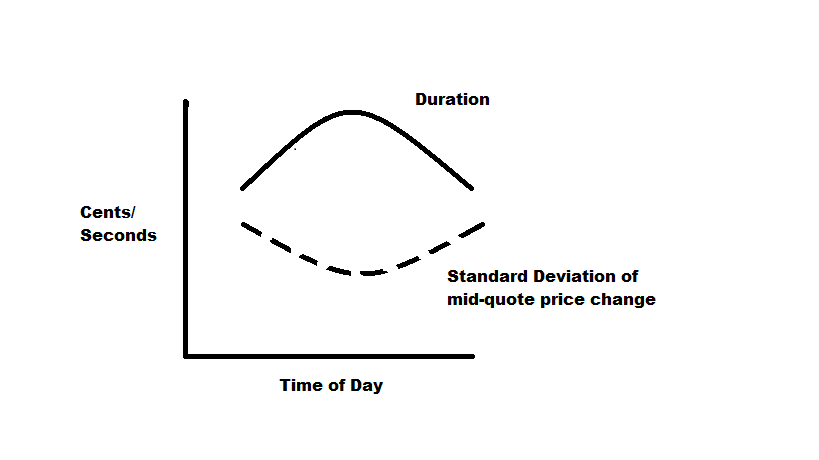
\includegraphics[width=\textwidth]{chapters/chapter_uvts/figures/Sec2-10Fig8.png}	
	\caption{Typical Diurnal patterns. \label{fig:diurnal}}
	\end{figure}

\item Volatility, volume, spread are higher near the open and close.

\item Time between trades, shorter near open and close.
\end{itemize}


\noindent\textbf{Stylized fact 6: Negative autocorrelation in returns:} Non-synchronous trading and bid-ask bounce both can introduce negative lag-1 autocorrelation in the returns. See Roll (1984)~\cite{????} and Lo and Mackinlay (1990)~\cite{lo1990}.


We want to briefly discuss the Roll model; on a typical day of trading stocks exhibit price changes numerous times. These changes signify merely the market friction, the friction between the demand and supply side and they are not necessarily due to true information about the stock. Assume that the true price (unobservable) follows a random walk model (\ref{eqn:?????}) as, 
	\begin{equation}\label{eqn:2plowstar}
	p_t^*=p_{t-1}^* + \epsilon_t 
	\end{equation}
and the observed price,
	\begin{equation}\label{eqn:2lowpstar}
	p_t = p_t^* + u_t
	\end{equation}
with `$\epsilon_t$' denoting the true information about the stock and `$u_t$' denoting the market friction. But the observed return,
	\begin{equation}\label{eqn:2firstrtlow}
	r_t=p_t-p_{t-1} = \epsilon_t + u_t - u_{t-1}
	\end{equation}
inducing the negative autocorrelation of lag 1 in the return due to the carry over term, `$u_{t-1}$'. The term on the right-hand side because of zero autocorrelation beyond lag-1 can be written as MA(1) model:
	\begin{equation}\label{eqn:2lowrt}
	r_t=a_t - \theta a_{t-1}
	\end{equation}
The value of `$\theta$' generally tends to be small, but nevertheless significant. 


\noindent \textit{Commonly used duration models:} The timing aspect of transaction was discussed in Easley and O'Hara (1992)~\cite{easley1992} and a rigorous set of tools was developed by Engle and Russell (1998)~\cite{engle1998}, as an alternative to fixed interval analysis. Treating the ticks as random variables that follow a point process, the intensity of transactions in an interval of length, $\Delta$, is defined as
	\begin{equation}\label{eqn:2lambda}
	\lambda(t) = \lim\limits_{\Delta \rightarrow 0}\frac{E[N(t+\Delta) - N(t)|F_t]}{\Delta}
	\end{equation}
where $N(t)$ denotes the number of ticks until `t' and $F_t$ is the information available until that time. The commonly used model for such arrival rates is Poisson that implies that the time between the two successive ticks is independent of pairwise ticks and follows an exponential distribution. But the duration data, $d_i = t_i - t_{i-1}$ exhibit some dependence, thus implying that time moves faster sometimes, faster than the clock time. The intensity rate, $\lambda(t)$ is not a constant, which is a typical characteristic of the exponential distribution. We briefly outline how the durations are modeled. For detailed discussion, see Tsay (2010)~\cite{tsay} or Lai and Xing (2008, Section 11.2)~\cite{lai1}. The autoregressive conditional duration (ACD) model is defined as follows:
	\begin{equation}\label{eqn:2dipsi}
	\begin{split}
	d_i&= t_i - t_{i-1} = \psi_i\varepsilon_i, \text{ and} \\
	\psi_i&= \alpha + \sum_{j=1}^p\alpha_j d_{t-j} + \sum_{v=1}^q\beta_v\psi_{i-v}
	\end{split}
	\end{equation}
where $\varepsilon_i$ are i.i.d. with $E(\varepsilon_i) = 1$; If $\varepsilon_t's$ are assumed to follow exponential the models (\ref{eqn:}) is called E(xpotential)ACD. Two alternative models WACD and GGACD are based on the following specification for the errors:
	\[
	\begin{split}
	\text{Weibull: }h(x) &= \frac{\alpha}{\beta^{\alpha}}x^{\alpha-1}\exp\left\{-(\frac{x}{\beta})^{\alpha}\right\} \\
	\text{Generalized Gamma: } y &= \lambda\frac{x}{\beta}
	\end{split}
	\]
where $\lambda = \frac{\sqrt{K}}{\sqrt{K+\frac{1}{\alpha}}}$. The hazard function of Generalized Gamma is quite flexible and may fit better various patterns. The stationary conditions would require that the roots of $\alpha(B) = 1 - \sum_{j=1}^q(\alpha_j+\beta_j)B^j$ are outside the unit circle when $g= \max(p,q)$ and $B$ is the back-shift operator. It is clear that the model (\ref{eqn:2dipsi}) is similar to GARCH$(p, q)$ model given in (\ref{eqn:}). The estimation is typically done through conditional maximum likelihood and all inferences are asymptotic.


An alternative more direct ARMA type model for log durations is suggested by Ghysels, Gourieroux and Jasiak (2004)~\cite{jasiak}:
\begin{equation}\label{eqn:21lnd}
	\ln{(d_i)} = \omega + \sum_{j=1}^p\alpha_j\ln{(d_{t-j})} + \sum_{j=1}^v\beta_j\varepsilon_{i-j} + \varepsilon_i
	\end{equation}
and $\varepsilon_i = \sqrt{h_i^v}u_i, h_i^v = \omega^v + \sum_{j=1}^{p^v}\alpha_j^v\varepsilon_{i-j}^2 + \sum_{j=1}^{q^v}\beta_j^vh_{i-j}^v$ where $u_i \sim N(0,1)$ i.i.d.; here the conditional mean and variance of durations are assumed to be separable. The duration volatility that is modeled using the second equation in (\ref{eqn:}) is interpreted as `liquidity' risk. \\


\noindent \textbf{Other Duration Related Models:} So far the discussion has been around modeling the durations, but the information set, $F_t$ has information on `marks', the information associated with the past ticks, such as the number of units transacted, price etc. McCulloch and Tsay (2009)~\cite{} suggest the following model:
	\begin{equation}\label{eqn:2lndi}
	\ln{d_i} = \beta_0 + \beta_1\ln{(d_{t-1})} + \beta_2s_{i-1} + \sigma\varepsilon_i
	\end{equation}
where $s_i$ is the size of the $i$th price change measured in ticks; other relevant variables can be easily added to this model.


\subsection{Models for Multiple Assets: High-Frequency Context}


There is a considerable interest in extending the univariate duration models to multiple stocks or to multiple types of arrival processes. Because investment managers generally consider a portfolio of stocks rather than a single one, it is important for them to follow the transaction processes of several stocks simultaneously. Because of non-synchronous trading relating two stocks with different trading intensities on a common time scale is somewhat difficult. Engle and Lunde (2003)~\cite{englelunde} establish the following model for a bivariate point process for trades and quotes:
	\begin{figure}[!ht]
	\centering
	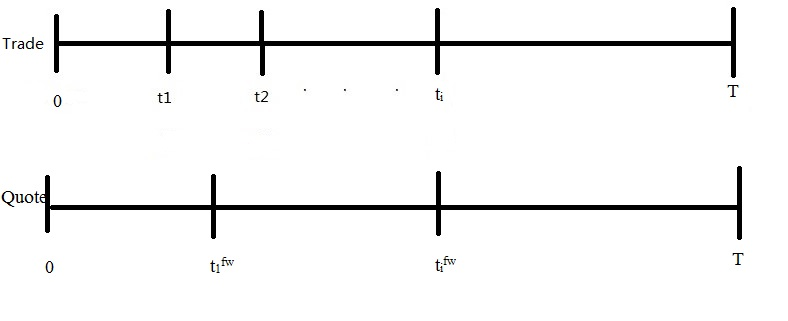
\includegraphics[width=\textwidth]{chapters/chapter_uvts/figures/33d3.jpg}
	\caption{Trades and Quotes. \label{fig:tradeactdoubline}}
	\end{figure}
Define $x_i = t_i - t_{i-1}$ as trade duration and $y_i = t_i^{f_w} - t_{i-1}^{f_w}$ as the forward quote duration; our goal is to model $(x_i,y_i)$ as a bivariate duration process but the underlying timings are not synchronized. Thus define, if $y_i > x_i$, then
	\begin{equation}\label{eqn:anothertildey}
	\widetilde{y}_i = (1 - d_i)y_i + d_ix_i
	\end{equation}
where $d_i$ is indicator variable, $d_i = I_{\{y_i>x_i\}}$. Model ($x_i,\widetilde{y}_i$) as censored process. The equation (98) provides a mechanism in a way to align the two processes. The joint distribution is given by
	\begin{equation}\label{eqn:2pxiyi}
	p(x_i,\widetilde{y}_i | F_{i-1},\omega) = g(x_i|F_{i-1},\omega_1) f(\widetilde{y}_i | x_i,F_{i-1},\omega_2)
	\end{equation}
The first term is the trade density and the second term is the quote density. The $\psi_i$ terms as in (\ref{eqn:}) are modeled as EACD, $\psi_i= f(\psi_{i-1},x_{i-1},z_{i-1})$ and quote density is also modeled as EACD after adjusting for censoring:
	\begin{equation}\label{eqn:2fdot}
	f(y_i|\cdot) = [h(y_i|\cdot)]^{1-d_i} \times S(x_i|\cdot)^{d_i}
	\end{equation}
The estimation of the parameters are done through quasi maximum likelihood. Using data for eight stocks, Engle and Lund (2003)~\cite{englelunde} observe that high trade arrival rates, large volume per trade, wide bid-ask spreads, all predict more rapid price revisions. The model given in Engle and Lund (2003)~\cite{englelunde} can be conceptually applied to any two point processes. Extending this concept to more than two processes could be of interest to the traders who may want to monitor the trading exchanges simultaneously. 


\section{Time Aggregation and Loss of Information}


\section{Realized Volatility and Econometric Models}


Estimating the volatility using the high-frequency data has received a great deal of attention lately. In the low frequency (daily) level some estimators based on select prices were presented. Intra-day dynamics of volatility is of interest to traders and that is not fully captured by the stock price indicators sampled during the day. If higher frequency data are used to estimate volatility of lower frequency data, it is important to know the model for the return at the lower frequency. To illustrate this, we consider data observed at two time scales; although they are at low frequency level, the concept can be easily extended to high-frequency context. If $r_{t,i}$ is the $i$th day return in $t$th month, the $t$th month return assuming there `n' trading days, $r_t^m = \sum_{i=1}^nr_{t,i}$. Note that $\sigma_m^2 = \Var(r_t^m|F_{t-1}) = \sum_{i=1}^n \Var(r_{t,i} | F_{t-1}) + 2 \sum_{i<j} \Cov(r_{t-i},r_{t-j} | F_{t-1})$. If $r_{t,i}$ is white noise sequence, then
	\begin{equation}\label{Eqn:2hatsigmasq}
	\hat{\sigma}_m^2 = \frac{n}{n-1} \sum_{i=1}^n(r_{t,i} - \overline{r}_t)^2
	\end{equation}
But we had observed that in the high frequency data returns do exhibit some serial correlation and so adjusting (\ref{eqn:}) for serial correlation is important to get a more accurate estimate of volatility. A simpler estimate of $\sigma_m^2$ is the so called realized volatility ($RV_t$)
	\begin{equation}\label{eqn:2RV}
	\text{RV}_t = \sum_{i=1}^n r_{t,i}^2
	\end{equation}
But in the estimation of intra-day volatility, the number of sampling intervals, `$n$' and hence, `$\Delta$', the interval size can affect the estimate. If $\Delta \rightarrow 0$, the value $RV_t$ in the $\Delta$-interval goes to infinity. Thus the optimal choice of `$\Delta$' is crucial and is reviewed below, for a judicious choice.


Bandi and Russell (2006)~\cite{bandi} argue that the observed price is the sum of efficient price and a friction price (see (\ref{eqn:})) that is induced by bid-ask bounce, price discreteness etc. Thus the observed variance such as (\ref{eqn:}) is the sum of variance of the efficient returns and the variance of micro-structure noise. As they indicate, both are useful: ``The variance of the efficient return process is a crucial ingredient in the practice and theory of asset valuation and risk management. The variance of microstructure noise components reflects the market structure and the price setting behavior of market participants and thereby contains information about the market fine-grain dynamics.'' Both components can be estimated using high frequency data but sampled at different frequencies. Data sampled at low frequency are used to estimate the efficient return variable and the data of high frequency are used to estimate the microstructure noise variance.


On any given day, assume that the observed price, at time `$i$' is as in (\ref{eqn:})
	\begin{equation}\label{eqn:2pi2}
	p_i = p_i^* + u_i, \quad i= 1,2,\ldots,n
	\end{equation}
where $p_i^*$ is the efficient price and $u_i$ is the of microstructure noise. Dividing a trading day into $M$ sub-periods, where $\delta= 1/M$ is the size of the sub-period, write the observed returns as
	\begin{equation}\label{eqn:2rji2}
	r_{j,i} = r_{j,i}^* + \varepsilon_{j,i}, \quad j= 1,2,\ldots,M
	\end{equation}
Assume that the frictions, $u$'s are i.i.d. mean zero and variance $\sigma_{u}^2$. Because $\varepsilon_{j,i}= u_{(i-1)+j\delta} - u{(i-1) + (j-1)\delta}$, $\Var(\varepsilon_{j,i})= 2\sigma_{\eta}^2$. It has been noted already that the return series exhibit negative first order autocovariance and $\varepsilon$'s can be taken as MA(1) structure for the $\eta$'s. Thus, the returns are computed at higher frequency at which the new information arrives. Thus $\sum_{j=1}^M r_{j,i}^2/M$ can be used to estimate noise variance. For the estimation of efficient price variance, we need to consider an  optimal division of a day into `M' number of subperiods. The optimal sampling frequency over `$n$' day is chosen as $\delta^* = 1/M^*$ with $M^*= \left[\dfrac{\hat{Q}}{\hat{\alpha}}\right]^{\frac{1}{3}}$, where $\hat{\alpha} = \sum_{i=1}^n\sum_{j=1}^M\overline{r}_{j,i}^2/(nM)$ and $\hat{Q}_i = \frac{M}{3}\sum_{j=1}^M\hat{r}_{j,i}^4$. Based on the analysis of a sample of S\&P 100 stocks mid quotes for the months of February 2002, Bandi and Russell (2006)~\cite{bandi} conclude that 5-min frequency is optimal and the 15-min interval may provide the variance estimates `excessively volatile'. The economic benefit of optimal sampling is that high frequency traders can employ a realistic variance forecasts in formulating the entry and exit strategies. Additional references on this topic include, A{\"\i}t-Sahalia, Mykland and Zhang (2005)~\cite{ait2005often} and Barndoff-Nielsen and Shepard (2002)~\cite{barndorff2002econometric}.


\section{Analytics from Machine Learning Literature}


The technical trading rules that are discussed in Chapter 3 involve a relatively small information set to carry out prediction. It treats each of the $n$ time series of asset returns as autonomous. As pointed out by Malkiel (2012)~\cite{malkiel}, these rules can be easily implemented by most market participants if such opportunities should emerge, and market efficiency would rule them out as winning strategies. More powerful prediction methods using a very large set of potential predictors and yet capable of avoiding overfitting are needed to take advantage of transient opportunities. We give a overview here of recent advances in high-dimensional regression and classification and in machine learning and computer science to handle different types of data (including text mining).




\section{Exercises}


The dataset consists of (CSV) file that contains the entire trading session, including early and late hours from 6:00~a.m. to 8:00~p.m. EST. It contains intraday depth book activity several major tickers from up to 5 major national exchanges: Nasdaq, Direct Edge, NYSE, ARCA, and BATS (exact number of exchanges depends on the historical period). All messages are consolidates into one file ordered by timestamp. This dataset allows to build a full national depth book (super book) at any moment intraday. 

\begin{table}[h!]
   \caption{Column Format}
   \centering
   \begin{tabular}{p{2cm}p{8cm}} 
   \textbf{Column} & \text{Description} \\ \hline
   Timestamp & Number of milliseconds after the midnight. \\ \hline
   Ticker & Equity symbol (up to 8 characters) \\ \hline
   Order & Unique order ID. \\ \hline
   T & Message type. Allowed Values: \newline
	~~\llap{\textbullet}~~ ``B''--Add buy order \newline
	~~\llap{\textbullet}~~ ``S''--Add sell order \newline
	~~\llap{\textbullet}~~ ``E''--Execute outstanding order in part \newline
	~~\llap{\textbullet}~~ ``F''--Execute outstanding order in full \newline
	~~\llap{\textbullet}~~ ``D''--Delete outstanding order in full \newline 
	~~\llap{\textbullet}~~ ``X''--Bulk volume for the cross event \newline
	~~\llap{\textbullet}~~ ``T''--Execute non-displayed order  \\ \hline
   Shares & Order quantity, available for the ``B'', ``S'', ``E'', ``X'', ``C'', ``T'' messages. Zero for ``F'' and ``D'' messages. \\ \hline
   Price & Order price, available for the ``B'', ``S'', ``X'', and ``T'' order messages. Zero for cancellation and executions. The last 4 digits are decimal digits. The decimal portion is padded on the right with zeros. The decimal point is implied by position; it does not appear inside the price field. Divide by 10000 to convert into currency value. \\ \hline
   MPID & Market Participant ID associated with the transaction (4 characters) \\ \hline
   MCID &U Market Center Code (originating exchange--1 character)
   \end{tabular}
\end{table}


For the analysis of Problems 1--3, we consider the data for CISCO.

\begin{enumerate}[1.]
 
\item You need to aggregate the data into 5-min intervals before answering the following.
\begin{enumerate}[(a)]
\item Let $x_t$ denote the number of trades in the $t$th 5-minute interval. Ignore the time gaps between trading days. Plot the time series and its ACF. Determine if there are intraday period patterns in the series.

\item Using the last transaction in the $t$th 5-minute interval as the stock price in that interval, plot the
time series $y_t$ of 5-minute returns during the period and the corresponding ACF.

\item Consider the bivariate time series ($x_t$, $y_t$). How does $y_t$ vary with $x_t$? Are there intraday periodic patterns in ($x_t$, $y_t$)?

\item Plot the durations of the transaction times for Mondays and Fridays. Is there any difference in the
patterns?

\item Fit GARCH models for the durations and interpret the coefficients.

\item Is there any particular exchange that offers better price?
\end{enumerate}



\item Use the transaction data in Problem 8. There are seventy-eight five-minute intervals in a trading day. Let $d_i$ be the average of all log durations for the $i$th 5-minute interval across all trading days. Let $t_j$ be tick time of a trade during the $i$th 5-minute interval, define an adjusted duration as $\Delta t_j^* = \Delta t_j/\exp(d_i)$ where $\Delta t_j = t_j - t_{j-1}$.
\begin{enumerate}[(a)]
\item Is there a diurnal pattern in the adjusted duration series?

\item Build EACD and WACD models for the adjusted duration and compare them. Now aggregate the data over the 5-minute intervals; Let $r_t$ be the return and $V_t$ is the volume of transactions in the $t$th interval.

\item Is there any relationship between the volume $V_t$ and volatility $r_t^2$ . If there is develop a model that will capture the dependence of volatility on volume. Let $\overline{p}_t$ be the average price in the $t$th 5-minute
interval.
\end{enumerate}


\item Use the CISCO execution data only; aggregate at various time intervals: 1~min, 2~min, \dots, 15~min. For these levels record
\begin{enumerate}[(a)]
\item Average price, VWAP, realized volatility and aggregate volume.

\item By relating the returns and volatility estimates based on average price to realized volatility, identify the optimal duration for aggregation that will cancel out the market friction but pick up the true information. (You may want to refer to Bandi and Russell (2006)~\cite{bandi}). 
\end{enumerate}

\end{enumerate}

\part{Trading Algorithms}
% !TEX root = ../../../book.tex

In Part~\ref{part:two}, our goal is to provide a review of some basic and some advanced statistical methodologies that are useful for developing trading algorithms. We begin with time series models (in Chapter~\ref{ch:ch_uvts}) for univariate data and provide a broad discussion of autoregressive, moving average models---from model identification, estimation, inference to model diagnostics. The stock price and return data exhibit some unique features and so we identify certain stylized facts regarding their behavior that have been empirically confirmed; this work will greatly help to discern any anomalies as and when they arise, as these anomalies generally indicate deviation from efficient market hypothesis. Although for modeling price and return data, only lower order models are needed, increasingly other trading features such as volume, volatility are being used in developing trading strategies. In particular,  predicting future volume flow to determine when to enter the market, requires the use of higher order models. Wherever possible we illustrate the methodology with examples and provide codes for computing, making the data accessible to the reader. We also introduce novel methodologies that have some potential for developing compelling trading models.


This chapter is followed by methodologies for multiple time series data in Chapter~\ref{ch:ch_mvts} which have applications from pairs trading to portfolio optimization. The last chapter (Chapter~\ref{ch:ch_advanced}) in Part~\ref{part:two} contains advanced topics such as theory of point processes as trading takes place on a continual basis. Finally, this chapter also contains a very brief treatment of other modern topics such as machine learning.


A reader with a strong statistics background can afford to skip some sections but we recommend to peruse these chapters as they contain discussions on topics that need further research work. In presenting the methodologies here, we keep the discussion lucid but immensely relevant to the main theme of this book---understanding the market behavior and developing effective trading strategies. 
% !TEX root = ../../book.tex
\chapter{Statistical Trading Strategies and Back-Testing}

\section{Introduction to Trading Strategies: Origin and History}

\noindent \textbf{Statistical arbitrage opportunity and strategies:} Trading strategies are central to the notion of statistical arbitrage. Strategies that claim to have better performance than the market date back to the inception of trading in finance. As we had already noted, there are a large number of studies that empirically conclude that the behavior of stock prices appear to contradict efficient market hypothesis. Broadly there are two types of strategies, one the momentum strategy that buys well-performing stocks and sells poor-performing stocks (see Jegadeesh and Titman (1993)~\cite{JeTit}) and the other, contrarian strategy that advocates buying past losers and selling past winners. The average excess return of some strategies relative to a standard capital asset pricing model is shown to be around 12\%. Other strategies, such as buying value and selling glamour stocks (see Lakonishok et al. (1994)~\cite{Lako}) use other company fundamental data such as price earnings ratios, dividends, book-to-market values, cash flows and sales growth.


Hogan, Jarrow, Teo and Warachka (2004)~\cite{Hogan} define `a statistical arbitrage as a long horizon trading opportunity that generates a riskless profit. Four conditions that are to be met are: it is a self-financing strategy with a zero initial cost, in the limit has positive expected discounted profits, a probability of a loss converging to zero and a time-averaged variance converging to zero; the last condition implies that an arbitrage opportunity eventually produces riskless profit. Citing anomalies to reject  market efficiency has been criticized on the ground that such tests depend upon a specified model for equilibrium returns. Hogan et al. (2004)~\cite{Hogan} argue that statistical arbitrage can be defined without any reference to an equilibrium model and rejects market efficiency. They provide a statistical test to determine if a trading strategy constitutes statistical arbitrage based on short horizon incremental profits. In this chapter we will cover some of these trading strategies and finally we will return to the proposed statistical test.


\section{Trading Rules for Time Aggregated Data}


Trading Rules that are broadly labeled as technical analysis involve the prediction of future short-term price movements from an inductive analysis of past movements using either quantitative techniques, such as moving averages or qualitative methods such as recognition of patterns from visual inspection of a time-series plot of the asset price data or a combination of both via semi-parametric procedures such as kernel smoothing. In foreign exchange market, as Menkhoff and Taylor (2002)~\cite{MalTay} observe the widespread use of these techniques is puzzling, ``since technical analysis eschews scrutiny of economic fundamentals and relies on information on past exchange rate movements that, according to the weakest notion of market efficiency, should already be embedded in the current exchange rate, making its use either unprofitable or implying that any positive returns that are generated are accompanied by an unacceptable risk exposure.'' In general there are economic fundamentals that can explain long term movements, there is still no fundamental-based exchange rate model that is capable of forecasting short-term movements.


Technical analysis (also known as Chartist analysis) is a set of techniques for obtaining forecasts based on past history of prices along with the history of trading volumes. Clearly for the technical analysis to be useful, price movements should follow some regular, recurring patterns and these patterns must hold for long enough periods to sustain the transaction costs and false signals so that the investment results in a profit. What constitutes a useful forecast from an investor point of view could be if the past history of prices can be used to increase expected gains. But as Fama and Blume (1966)~\cite{famablume} point out, ``In a random walk market, with either zero or positive drift, no mechanical trading rule applied to an individual security would consistently outperform a policy of simply buying and holding the security''. The past movements could be useful only when there is some degree of dependence in successive price changes. The serial correlation measures may not capture the complex dependence that may exist. In what follows we briefly describe some commonly used trading rules and comment on their noted performance.


\subsection{Filter Rules}


Alexander (1961, 1964)~\cite{} studied the filter technique that is intuitive and is easy to implement; the basic idea is summarized below: \\


\noindent \textbf{x\% Filter:} If a daily closing price moves up at least x\% from its past low, buy and hold, until its price moves down at least x\% from a subsequent high, sell and go short. Maintain the short position until price rises at least x\% above a subsequent low, buy. Moves less than x\% in either direction are ignored. \\


The general logic behind this rule is that if the price moved up $x$\%, it is likely to move up more than $x$\% further before it moves down by $x$\%; Thus the random walk model is not likely to be upheld by the data. As observed by Mandelbrot (1963)~\cite{}, because of the price jumps that occur at the time of transaction, the purchase price and sale price will not exactly match as required by the rule.


The initial application of this rule on daily data for S\&P industrials showed that the trading rules with 5, 6 and 8\%. filters generated larger gross profits than the buy and hold strategy. This study did not account for the transaction cost. But a later study that incorporated a commission of 2\% for each round-trip, only the larger filter  $\sim$ 46\% rule beat the buy and hold strategy and all the other filters adjusting for the transaction costs did not perform better than simply buying and holding.


Fama and Blume (1966)~\cite{famablume} after applying Alexander's filter technique for each of the individual security in Dow Jones Industrial Average for the daily data during a five year period, 1957--1962, concluded, ``When commissions are taken into account, the larger profits under the filter technique are those of the brokers. When commissions are omitted, the returns from the filter techniques are, of course, greatly improved but are still not as large as the returns from simply buying and holding.'' It is argued that under random walk model, the average return on long positions should be approximately equal to the buy and hold average returns. This may not be true if the drift occurs at the time of entry or exit; the filter rule can be stated under RW Model as follows; let the return, $r_{t} = \ln{P_{t}} - \ln{P{t-1}} = \mu_{t} + a_{t}$, when $a_{t} \sim$ N(0,$\sigma_{P}^2$) and `$\mu_{t}$' is the random drift term and $\sigma_{P}^2$ is the volatility; as for the filter rule, enter if $r_{t} > r$ and suppose this occurs at time $t_{0}$. If the drift term is approximately picked up at time `$t_{0}$', so that $\mu_{t} = 0$, for $t < t_{0}$ but $\mu_{t} = \mu > 0$ for $t \geq t_{0}$, the returns from the filter should fare better. The lasting of the drift is to be carefully monitored and using the exit strategy when $r_{t} < r$ will guarantee any undue losses.


When the filters are small it has been observed that there is evidence of positive dependence in returns and it may be useful to predict only short term dependence. This may signal opportunities for more frequent transactions but the cost of transactions as mentioned earlier can eat away the profits.


Sweeney (1998)~\cite{sweet} develops a test for risk-adjusted filters profits. The stocks considered in Fama and Blume (1966)~\cite{famablume} that are ``winners'' in one period tend to persist as winners in later periods. Thus focusing only on winners rather than entire set of stocks gives better results. Assume that the investor uses the filters rule each day to decide to enter or exit based solely as past information. Consider the span of $N$ days and with a filter strategy, the asset is held on $N_{\text{in}}$ days and is not held on $N_{\text{out}}$ days. At the end of $N$ days, the filter's performance is evaluated. The average excess rate of buy and hold is
	\[
	\overline{R}_{BH}=\dfrac{1}{N} \sum_{i=1}^N \, (r_t - r_f )
	\]
where $r_t$ is the stock's rate of return in period `$t$' and $r_f$ is the risk free rate. Assume that `$f$' is the proportion of days, the asset is not held; then the average excess rate of the filter is
	\[
	\overline{R}_{F}=\dfrac{1-f}{N_{in}}\sum_{t \in I} (r_t - r_f) 
	\]
Assume that under any of the asset pricing models (CAPM, APT etc.) expected excess rate of return equals a constant risk premium, $PR_{j}$. Note $E(\overline{R}_{BH}) = PR$ and $E(\overline{R}_{F}) = (1-f)PR$; Use the adjusted statistic
	\begin{equation}\label{eqn:xbarfirst}
	x= \overline{R}_{F} - (1-f)\overline{R}_{BH}
	\end{equation}
to judge the filter rule; observe $E(x) = 0$ and $\sigma_{x} = \sigma[\frac{f(1-f)}{N}]^{1/2}$, where `$\sigma$' is the standard deviation of excess return $r_t - r_f$. Fama and Blume (1966)~\cite{famablume} use
	\begin{equation}\label{eqn:bigxbar}
	X = \overline{R}_{FI} - \overline{R}_{BH}
	\end{equation}
where $\overline{R}_{fI} = \frac{1}{N_{in}}\sum_{t\in I}(r_t - r_F)$; Note $E(X) = 0$ and $\sigma_{x} = \sigma_{X}$.


The main advantage of $X$ is that it measures profits for each day in the duration of `$N$' days and $x$ measures profits per day for those days when the stock is held. The above results hold for the case of time varying risk premia as well; Suppose
	\[
	r_f - r_f = PR + a_t
	\]
where $a_t$ is stochastic; thus
	\begin{equation}\label{eqn:anotherxeq}
	x = \dfrac{1}{N_{in}} \sum_{t \in I} a_t - \dfrac{1}{N} \sum_{t=1}^N a_t + (\overline{PR}_{N_{in} }+\overline{PR}_N )
	\end{equation}
If the investor has no insight into changes in risk premia, then $E(\overline{PR}_{N_{in}}-\overline{PR}_{N}) = 0$; If the investor has no insight about the stochastic, $a_t$, the filter rule may be forecasting the risk premia.


It has been pointed out that Fama and Blume measure is biased against finding successful filter rules. The statistics X and x are meant for long strategies where the investor has the funds in the risk free asset when not holding. If we define,
	\[
	\overline{R}_{F'} = \dfrac{1}{N} \left( \sum_{t\in I} (r_t - r_f) - \sum_{t \in O} (r_t - r_f) \right)
	\]
and $E(\overline{R}_{{F}'} - \overline{R}_{BH}) = (1 - 2f) PR - PR = -2f PR$, a proportion of constant risk premium, thus resulting in a bias.


\subsection{Moving Average Variants and Oscillators}


The moving average trading rules are generally based on comparing the current price with the current moving average. Consider the prices, $P_t, P_{t-1}, \ldots, P_{t-m+1}$ with a moving window of width `$m$'. Various versions of moving average are available in the literature; 
	\begin{equation}\label{eqn:multi}
	\text{(SMA) Simple Moving Average: } \overline{P}_t^{(m)}= \dfrac{1}{m} \sum_{i=0}^{m-1} P_{t-i} \hfill
	\end{equation}
	\begin{equation*}
	\begin{split}
	&\text{(EWA) Exponentially Weighted Average: } \overline{P}_t^{(m)} = \left(\dfrac{1}{\sum_{i=0}^{m-1} \lambda^{i+1}} \right) \sum_{i=0}^{m-1} \lambda^{i+1} P_{t-i} \\
	&\text{(BWA) Bollinger Weighted Moving Average: }  \hat{P}_t^{(m)}= \left(\dfrac{1}{\sum_{i=1}^m}\right) \sum_{i=0}^{m-1} (m-i) P_{t-i}
	\end{split}
	\end{equation*}
The indicators of the above kind will tend to be profitable in markets that exhibit definite trends and so they are generally known as ``trend-following'' or some times, called as ``momentum'' indicators. Some simple rules that are normally used in practice are: \\[0.1cm]
\noindent\fbox{%
    \parbox{\textwidth}{%
	\textbf{SMA Rule: If } $\mathbf{\frac{\overline{P}_{t}^{(m)}}{P_{t}} > U} \textbf{ or }\mathbf{<L,}$ \textbf{ trade;} \\
	\textbf{EWA Rule: If } $\mathbf{\frac{\overline{P}_{t}^{(m)}(\lambda)}{P_{t}} > U} \textbf{ or }\mathbf{<L,}$ \textbf{ trade}
    }%
} \\

The two types of potential strategies are broadly known as ``Contrarian'' vs ``Momentum'' and they differ mainly on when the entry is carried out. The contrarian in a way looks for local minimum to enter the market and the momentum follower looks for a local maximum to enter.


While the above rules are easy to implement and one may observe that they do not take into account the variance or the volatility of the price (return) process. The widely used Bollinger band, conceptually similar to monitoring the quality of a manufacturing process, is based on the weighted moving average and the variance. Define $\hat{\sigma}_{t}^{(m)} = \{\frac{1}{m-1}\sum_{i=0}^{m-1}(P_{t-i} - \overline{P}_{t}^{(m)})^2\}^{1/2}$ and the rule can be stated as follows: \\[0.1cm]
\noindent\fbox{%
    \parbox{\textwidth}{%
	\textbf{Bollinger Rule: If }$\mathbf{P_{t} > P_{t}^+ = \hat{P}_{t}^{(m)} + 2\hat{\sigma}_{t}^{(m)}}$\textbf{, the upper band, then sell; buy if } $\mathbf{P_{t} < P^- = \hat{P}_{t}^{(m)} - 2\hat{\sigma}_{t}^{(m)}}$ \textbf{, the lower band, then buy; No action is taken in-between.}
    }%
} \\


Broadly the key qualities such as moving average, weighted or exponentially weighted average etc. correspond to the running-mean smoother discussed in Lai and Xing (2009, Section 7.2.1)~\cite{lai1}. Instead of the running-mean, some technical rules use the running maximum (i. e $\max\limits_{0 \leq i \leq m} P_{t-i}$) and the running minimum (i. e $\min\limits_{0 \leq i \leq m} P_{t-i}$) in the above rules. \\


\noindent \textbf{Moving Average Oscillator:} The use of the technical rules by the foreign exchange professionals is well documented (See Menkhoff and Taylor (2007)~\cite{MalTay}). The so called moving average oscillator rule requires computing two moving averages of short and long time spans. Let $\overline{P}_{t}^{(m)}$ and $\overline{P}_{t}^{(n)}$be the short and long averages, where $m< n$. The rule would signal a break in trend when the longer moving average is crossed by a shorter moving average (or spot rate). The upward trend is signaled when short moving average intersect from below the long average. Conversely a downward break in trend is signaled if the crossing occurs from above. Precisely the rule is: \\[0.1cm]

\noindent\fbox{%
    \parbox{\textwidth}{%
\noindent\textbf{Oscillator Rule: }\\

\noindent\textbf{Enter if } $\mathbf{\overline{P}_{t-1}^{(m)} < \overline{P}_{t-1}^{(n)}}$ \textbf{ and } $\mathbf{\overline{P}_t^{(m)} > \overline{P}_t^{(n)}}$ \\

\noindent\textbf{Exit if }$\mathbf{\overline{P}_{t-1}^{(m)} > \overline{P}_{t-1}^{(n)}}$ \textbf{ and }$\mathbf{\overline{P}_t^{(m)} < \overline{P}_t^{(n)}}$ \\
    }%
} \\


\noindent \textbf{RSI Oscillator:} Another oscillator that is designed to measure the strength of price movement in a particular direction is the relative strength indicator (RSI). The logic being that if the changes are too rapid in one direction, a correction in the opposite direction is likely to occur soon. Thus these types of rules are called `reversal' or `overbought/oversold' indicators. To define RSI, let $U_{t} = \sum_{i=1}^m I(P_{t-i} - P_{t-i-1} > 0)\,|P_{t-i} - P_{t-i-1}|$ and $D_{t} = \sum_{i=1}^m I_{t}(P_{t-i} - P_{t-i-1} < 0)\,|S_{t-i} - S_{t-i-1}|$ where $I(\cdot)$ is an indicator function. Thus $U_t$ and $D_t$ aggregate the positive and negative side of the price changes. Now let $RS_{t} = \frac {U_{t}}{D_{t}}$ and define
	\begin{equation}\label{eqn:rsi}
	RSI_{t} = 100 \times \frac{U_{t}}{U_{t}+D_{t}} = 100 - 100\left(\dfrac{1}{1+RS_t}\right)
	\end{equation}
By construction, RSI is normalized to lie between 0 and 100. \\[0.1cm]


\noindent\fbox{%
    \parbox{\textwidth}{%
\noindent \textbf{Reversal Rule:} \\

\noindent\textbf{If }$\mathbf{RSI_{t} > 70}$\textbf{, it is overbought signaling a downward correction and hence exit or short sell.} \\

\noindent\textbf{If }$\mathbf{RSI_{t} < 30}$\textbf{, it is oversold signaling an upward correction and hence enter.} \\
    }%
} \\


These rules that appear to be somewhat ad hoc can all be related back to the random walk model (see Chapter 2) with a drift:
	\begin{equation}\label{eqn:anotherpt}
	p_t = \mu+p_{t-1}+a_t
	\end{equation}
where $a_t \sim \text{N}(0,\sigma^2), \sigma^2$ is the volatility of the stock and note $r_t=p_t-p_{t-1}$; thus  $r_t \sim \text{N}(\mu,\sigma^2)$. If there is any autocorrelation in `$r_t$', and if $\overline{r}_n$ is the average based on the last `$n$' observations, then $\overline{r}_n \sim \text{N}\left(\mu,\sum_{\mid h \mid < n}\left(1-\frac{\mid h \mid}{n}\right)\frac{\gamma(h)}{n}\right)$, where $\gamma(h)$ is the autocovariance function of lag `$h$', with $\gamma(0)=\sigma^2$. When $\gamma(h)=0 \text{ for } h>0$, that P($\overline{r}_n>0)=\text{P}(\overline{a}_n>-\mu)=\text{P}\left(\frac{\overline{a}_n}{\sigma}>\frac{-\mu}{\sigma}\right)=1-\Phi\left(-\frac{\mu}{\sigma}\right)$ where $\Phi$ is the c.d.f. of the standard normal distribution. Thus we can evaluate $RS_t$ by the odds ratio, $\frac{1-\Phi\left(-\dfrac{\mu}{\sigma}\right)}{\Phi\left(-\frac{\mu}{\sigma}\right)}$. In fact the reversal rule stated above implies for $RSI_t$ to be greater than 70, $RS_t>2.33$. All the rules stated in this section can be written in the form of the c.d.f. of the underlying distribution of the return. This model-based interpretation of the rules can help us in accommodating other factors such as volume more formally in the model. 


\section{Patterns Discovery via Non-Parametric Smoothing Methods}


Charting has been a part of financial practice for many decades; but because of its highly subjective nature of interpretation of geometric shapes in price series, reading charts is ``often in the eyes of the beholder''. Lo, Mamaysky and Wang (LMW) (2000)~\cite{LoMWang} propose a systematic approach to pattern recognition using nonparametric kernel regression. The general goal of this analysis is to identify regularities in the price series by extracting nonlinear patterns. The smoothing estimators that can perform the signal extraction by averaging out the noise are ideally suited for this task.	


Assume that prices follow,
	\begin{equation} \label{eqn:4pt}
	P_{t} = m(x_{t}) + a_{t}
	\end{equation}
where $m(x_{t})$ is an arbitrary function of the state variable, $X_{t}$. For most practical purposes, assume $X_{t}= t$. Kernel regression, orthogonal series expansion, projection pursuit, neural networks are all examples of smoothing methods that are applied to estimate $\hat{m}(x_{t})$;
	\begin{equation}\label{eqn:4mx}
	\hat{m}(x) = \frac{1}{T}\sum_{t=1}^Tw_{t}(x)P_{t}
	\end{equation}
where the weights $\{w_{t}(x)\}$ are large for those $P_{t}$'s paired with $x_{t}$'s near $x$ and are small for those away from $x$. The weight function in (\ref{eqn:4mx}) is defined for a neighborhood of width `$h$'  around `$x$' can be defined as
	\begin{equation}\label{eqn:3mhat}
	\hat{m}_{h}(x) = \frac{1}{T}\sum_{t=1}^T w_{t,h}(x)P_{t} = \dfrac{\sum_{t=1}^T K_{h}(x-x_{t})P_{t}}{\sum_{t=1}^T K_{h}(x-x_{t})}
	\end{equation}
where $K(x)$ is a probability density function and is also called as `Kernel', and $\hat{m}_{h}(x)$ is called Nadaraya-Watson kernel estimator. A popular estimator is the density of a standard normal distribution, $K(t)=\frac{e^{-t^2/2}}{\sqrt{2\pi}}$.


Selecting the appropriate bandwidth, `$h$' is important as a small `$h$' may not smooth much and a large `$h$' may result in too smooth a graph. The choice of `$h$' is made through cross-validation, by minimizing
	\begin{equation}\label{eqn:cvh}
	\text{CV}(h) = \frac{1}{T}\sum_{t=1}^T (P_{t} - \hat{m}_{h}(t))^2
	\end{equation}
where
	\begin{equation}\label{eqn:mht}
	\hat{m}_{h,t} = \frac{1}{T}\sum_{\tau\not=t}^T w_{\tau,h}P_{\tau}
	\end{equation}
Thus the bandwidth choice depends on how well the estimator fits each observation, $P_{t}$, when it is not used in the construction of a Kernel estimator. LMW(2000)~\cite{LoMWang} observe that generally the bandwidth choice made through (\ref{eqn:cvh}) when applied to price series, tend to be larger and they suggest using $0.3\times h$.

To automate the detection of charting patterns, first the pattern is defined in terms of its geometric properties, then $\hat{m}(x)$ is estimated via (\ref{eqn:3mhat}), to match with it. LMW(2000)~\cite{LoMWang} define ten different patterns based on local extremes. The window size is $(t,t+l+d-1)$, where $l$ and $d$ are fixed parameters, so that a pattern is completed within $l+d$ trading days.


Within each window, estimate  a kernel regression using prices in that window:
	\begin{equation}\label{eqn:longhat}
	\hat{m}_{h}(\tau) = \dfrac{\sum_{s = t}^{t+l+d-1}K_{h}(\tau - s)P_{s}}{\sum_{s = t}^{t+l+d-1}K_{h}(\tau - s)}, \quad t = 1,\ldots , T-l-d-1
	\end{equation}
and the local extremes are identified through sign changes in $\hat{m}_{h}(\tau)$.


To test if the kernel regression yields better prediction, LMW(2000)~\cite{LoMWang} compare the unconditioned distribution of returns to the conditioned distribution, conditioned on the existence of a pattern. These comparisons are made through a goodness-of-fit test and Kolmogrov - Smirnov test. It  is generally found that the Kernel regression method yields somewhat better predictions. Jegadeesh (2000)~\cite{Jeqa} in his discussion of LMW(2000)~\cite{LoMWang} questions if the chartists' belief that selected patterns of the past tend to repeat as there is a great deal of noted subjectivity in the interpretation of charts. It is further noted that the practitioners tend to use the visual patterns in conjunction with other information such as macro level events that exert large influence compared to stock specific moves, to time their trades.


\section{A Decomposition Algorithm}


The rules that were discussed in previous sections are mostly trend following and use the past price or returns data. The predictability of returns generally tends to be weak. But the direction of change and volatility of returns tend to exhibit somewhat stronger dependence over time. Anatolyev and Gospodinov (2010)~\cite{Ananto2} exploit this and decompose the returns into a product of sign and absolute value components whose joint distribution is obtained through a model for absolute value of the return and a binary choice model for direction of the return and a copula for their interaction. Precisely the returns, `$r_{t}$', is written as
	\begin{equation}\label{eqn:3sgn}
	r_t = c + |r_t - c| \sgn (r_t - c)= c + |r_t - c| (2\cdot I(r_t >c) - 1)
	\end{equation}
where $I(r_t > c)$ is an indicator function. The values of $c$ are determined by the user; it could be a multiple of the standard deviation of `$r_{t}$' or it could represent the transaction cost or the risk free rate. This model is conceptually similar to Rydberg and Shephard (2003)~\cite{Ryd} and potential usefulness of the decomposition is also mentioned in Anatoleyev and Gerko (2005)~\cite{Ananto1}.


An advantage of the decomposition can be illustrated as follows. Assume for convenience, $c = 0$. From the model for $|r_t|$ and $I(r_t > 0)$, write $E_{t-1}(\left|r_{t}\right|) = \alpha_{\left|r\right|} + \beta_{\left|r\right|}\text{RV}_{t-1}$ and $Pr_{t-1}(r_t >0) = \alpha_{\left|I\right|} + \beta_{\left|I\right|}RV_{t-1}$, where RV denotes the realized volatility and $E_{t-1}(r_t)= -E_{t-1}(\left|r_t \right|) + 2E_{t-1}(\left|r_{t}\right| \cdot I(r_{t} > 0))=\alpha_{r} + \beta_{r}RV_{t-1} + \sigma_{r} RV_{t-1}^2$.


Thus, the decomposition in (\ref{eqn:3sgn}) results in accommodating non-linearity and the model can include other asset related variables. Hence any dynamic modeling that captures the hidden non-linearities is likely to improve the prediction of $r_{t}$. With the random walk model for price, $r_t$ is taken to be white noise, but the above formulation helps to capture any time dependence. We describe below some useful formulations.


The marginal distributions of the absolute value and sign terms are modeled as follows.
	\begin{equation}\label{eqn:psieta}
	\left|r_{t} - c \right| = \psi_{t}\eta_{t}
	\end{equation}
where $\eta_{t}$ is Weibull distribution and
	\begin{equation}\label{eqn:lnspi}
	\ln{\psi_{t}} = w_{v} + \beta_{v}\ln{\psi_{t-1}} + r_{v}\ln{|r_{t-1}-c|} + \rho_{v}I(r_{t-1}>c) + x'_{t-1}\delta_{v}
	\end{equation}
Note the above specification is the same as the autoregressive conditional duration (ACD) model. The $x_{t}$'s  are macroeconomic predictors that may have an effect on volatility dynamics. The specification of the indicator variable is done as follows: The indicator variable $I(r_{t} > c)$ is assumed to follow Bernoulli($p_{t})$, where $p_{t} = logit(\theta_{t})$, where 
	\begin{equation}\label{eqn:3thetat}
	\theta_{t} = w_{d} + \phi_{d}I (r_{t-1}>c) + y_{t-1}'\delta_{d}
	\end{equation}
where $y_{t}$'s can, besides the macro economic variables, include the realized variance, $\text{RV}_{t} = \sum_{s=1}^{m} r^2_{t,s}$, bipower variation, $\text{BPV}_{t} = \frac{\pi}{2} \cdot \frac{m}{m-1} \cdot \sum_{s=1}^{m-1} \left|r_{t,s}\right| \left|r_{t,s+1}\right|$ and the realized third and fourth moments, $\text{RS}_{t} = \sum_{s=1}^m r_{t,s}^3$ and $\text{RK}_{t} = \sum_{s=1}^{m}r_{t,s}^4$.


With the marginals specified as above with the corresponding, c.d.f.'s $F(\cdot$), the joint density is given as
	\begin{equation}\label{eqn:frt}
	F_{r_t}(u,v) = c [F_{|r_t-c|}^{(u)}, F_{I(r_t>0)}^{(v)}]
	\end{equation}
where $c(w_1,w_2)$ is a Copula, a bivariate c.d.f.. For a general discussion on Copulas refer to Lai and Xing (2008, Section 12.3.3)~\cite{lai1}.


In the trading context, the value of a strategy to buy or sell depends on how good the short term prediction of $r_{t}$ is. Note that the conditional mean can be expressed as,
	\[
	E_{t-1}(r_t) = c - E_{t-1}(\left|r_t - c\right|) + 2E_{t-1}(\left|r_t - c\right| I(r_t - c))
	\]
Hence,
	\begin{equation}\label{eqn:hatrt}
	\hat{r}_{t} = c - \hat{\psi}_{t} + 2\hat{\varepsilon}_t
	\end{equation}
where $\varepsilon_t$ is the expected value of the cross product term in $E_{t-1}(r_t)$. If the cross-product terms are conditionally independent, $\varepsilon_t = \psi_t p_t$ and thus
	\begin{equation}\label{eqn:hatrt2}
	\hat{r}_t = c + (2\hat{p}_t - 1)\hat{\psi}_t
	\end{equation}
Thus the prediction of $r_{t}$ includes both the directional and volatility predictions.


A possible strategy is to invest in stocks if the predicted excess return is positive or invest in bonds if it is negative. In term of established measures of performance, the decomposition method is shown to yield somewhat superior results. \\


\noindent \textbf{Other Non-Linear Models:} There has been some interest in using Neural Networks for developing technical rules that have better predictive power than the baseline models such as random walk or the following AR($p$) model:
	\begin{equation}\label{eqn:ri}
	r_t = \alpha + \sum_{i=1}^p\phi_ir_{t-i} + a_t 
	\end{equation}
where $a_t \sim N(0, \sigma_a^2)$. This model is augmented with term used in oscillator rule that was discussed earlier. Define $s_t^{m,n} = P_t^m - P_t^n$, the oscillator signal resulting from the short and long term moving averages of the prices and the model,
	\begin{equation}\label{eqn:rtsum}
	r_t = \alpha + \sum_{i=1}^p\phi_ir_{t-i} + \sum_{i=1}^p\eta_is_{t-i}^{m,n}+ a_t
	\end{equation}
is an extended linear model and is shown to increase the predictive power. The feed forward neural network model with `$d$' hidden units is written as
	\begin{equation}\label{eqn:rtsum2}
	r_t = \alpha_0 + \sum_{i=1}^p \phi_{ij}r_{t-i} + \sum_{j=1}^d \eta_j G\left[\alpha_j + \sum_{i=1}^pr_{ij}s_{t-i}^{m,n} \right] + a_t
	\end{equation}
where the activation function $G(x) = \dfrac{1}{1 + e^{-\alpha x}}$ is of the logistic functional form. Gencay(1998)~\cite{gencay} examining the daily Dow Jones Industrial Average Index from 1877 to 1998 finds the evidence of nonlinear predictability in returns by using the oscillator signals.


\section{Fair Value Models}


The trading strategies are typically evaluated by comparing their performance against some benchmarks. Traders often face challenges to find trading opportunities that will outperform these benchmarks. In the model considered in Section 3.4, the quantity, `$c$' is taken to be transaction cost or simply it can be set to risk-free rate. The fair value models are based on the assumption that the fair price of a stock is influenced by some common factors. These factors are general market factors; examples of the linear factor models of returns are CAPM, Fama-French three and five factor models and Carhart factor models. As consistent with algorithmic trading principle, large deviations that are not explained by the dynamics of the established factors are taken to be abnormal and can be exploited as trading opportunities.


For the CAPM model, where $r_t$ is the return on the asset, $r_{mt}$ is the market return, and $r_f$ is the risk-free rate,
	\begin{equation}\label{eqn:rtmrf}
	r_t - r_f = \alpha + \beta \,( r_{mt} - r_f ) + e_t
	\end{equation}
it is expected that $\alpha=0$ if the model holds. Any deviation from the null hypothesis $H_0:\alpha=0$ indicates the adjusted stock performance after adjusting for the risk-return relationship. In addition it is expected in a high-frequency setting, $e_t$'s are likely to exhibit some serial dependence:
	\begin{equation}\label{eqn:et}
	e_t = a_t - \theta a_{t-1}
	\end{equation}
Estimating the model parameters can be accomplished by the methodology given in Chapter 2; the procedure is generalized least squares and is iterative. The model in (\ref{eqn:rtmrf}) can be extended to include other factors to provide a general model:
	\begin{equation}\label{eqn:rtalpha}
	r_t = \alpha + \beta'f_{t} + e_t
	\end{equation}
where $f_t$ is an `$n$'-dimensional vector of factors that may include in addition to the market index, $\text{SMB}_t$, the return on diversified portfolio of small stocks minus the return on a diversified portfolio of big stocks, $\text{HML}_t$ is the difference between the returns on diversified portfolios of high and low Book to Market (B/M) stocks, $\text{RMW}_t$ is the difference between the returns on diversified portfolios of stocks with robust and weak profitability and $\text{CMA}_t$ in the difference between the returns on diversified portfolios of the stocks of low (conservative) and high (aggressive) investment firms (see Fama and French (2015)~\cite{fama2015}). Carhart (1997)~\cite{carhart1997persistence} in studying the persistence of mutual fund performance uses one-year momentum in stock returns as an additional factor to Fama and French's original three factor model.


A general comment is in order: the so called factors mostly meant for explaining cross-sectional variation are slow-moving and hence the only factor that is likely to change in the high frequency context is the market factor. Also the error term may contain mostly the information about the market friction and hence the model (\ref{eqn:rtmrf}) may itself not be reliable.


\section{Back-Testing and Data Snooping:  In-Sample and Out-of-Sample Performance Evaluation}


With the publication of an influential paper by Brock, Lakonishok and LeBaron (1992)~\cite{BLL} on technical rules, the main stream finance academics have started paying attention to studying the properties of these rules. The rules considered are moving average and trading range break and applying these rules on the Dow Jones Index from 1897 to 1986, they show that technical strategies perform very well. Results they obtain are not consistent with the usual benchmark models: the random walk, AR(1), GARCH-M and Exponential GARCH. Buy signals generally tend to fare better. The p-values for the rules are estimated through Bootstrap method. But Ready(2002)~\cite{ready} argues that the apparent success after transaction costs of the Brock et al. (1992)~\cite{BLL} moving average rules is a spurious result of data snooping. It's shown that the rules did poorly post 1986 and the average returns for 1987--2000 were higher on days when strategies suggest to be out of the market.


Data snooping occurs if the same data is used for both model selection and model validation. The significant results obtained can be due to pure chance. As Sullivan, Timmermann and White (1999)~\cite{sullivan1999data} suggest the data snooping may be due to survivorship bias as only successful trading rules tend to be replicated. Thus it is important to consider the almost entire universe of trading rules to study the snooping bias.


Sullivan et al (1999)~\cite{sullivan1999data} suggest using a bootstrap procedure studied in White (1999)~\cite{white1999} to check on data snooping bias. The bias comes mainly from the application of multiple trading rules on the same set of data and thus by pure chance can yield significant results. If there are `$l$' trading rules under consideration and they are validated over next `$n$' periods, define
	\begin{equation}\label{eqn:barf}
	\overline{f}= \frac{1}{n}\sum_{j=1}^n\hat{f}_{t+j}
	\end{equation}
where $\hat{f}_{t+j}$ is the observed performance measure for period `$t+j$', based on the data up to `$t$'. For the $k$th trading rule, let
	\begin{equation}\label{eqn:fktj}
	f_{k,t+j}= \ln(1+r_{t+j} s_k) - \ln(1+r_{t+j} s_0)
	\end{equation}
where $r_{t+j}$ is the return, $s_k$ and $s_0$ are signal functions for the $k^{th}$ trading rule and the baseline or benchmark rule, that can take three positions: long, short and neutral, taking values 1, $-1$, and zero, respectively. The signal functions are of course based on data and information available as of '$t$'. The proposed test assumes the null hypothesis that the best technical rule does no better than the benchmark rule:
	\begin{equation}\label{eqn:H0}
	H_0: \max_{k=1,\ldots,l}E(f_k) \leq 0
	\end{equation}
Rejection of $H_0$ would establish that the best technical rule is superior to the benchmark rule. Hypothesis similar to (\ref{eqn:H0}) can be formulated for the Sharpe ratio as well which will be a risk-adjusted measure. The $p$-values for $H_0$ are obtained through Bootstrap resampling procedures, to construct the following statistics:
If there are `$B$' bootstrapped values of $\overline{f}_k$ denoted by $\overline{f}_{k,i}^*, i=1,2,...B$ construct the following statistics:
	\begin{equation}\label{eqn:linev}
	\overline{v}_l = \max_{k=1,\ldots,l} \{\sqrt{n}\;\overline{f}_k\}
	\end{equation}
	\begin{equation}\label{eqn:linevli}
	\overline{v}_{l,i} = \max_{k=1,\ldots,l} \{\sqrt{n}\,(\overline{f}_{k,i}^* - \overline{f}_k) \}
	\end{equation}
The values of $\overline{v}_l$ are compared to the quantities of $\overline{v}_{l,i}^*$ to obtain the $p$-values.


The number of trading rules, $l=7846$, considered by Sullivan et al (1999)~\cite{sullivan1999data} is fairly exhaustive. The benchmark rule is being `always out of the market.' The difference between the two $p$-values, i.e. between the Bootstrap resampling method and the nominal method is fairly substantial for the out-of-sample periods for the universe of trading rules considered. However, there are certain trading rules that are found to outperform the benchmarks both in terms of the average return and the Sharpe ratio.


Two main drawbacks of the above test are: one the test is conservative and may lose power when poor performing models are included in the universe of the tests; second the test does not identify other significant models other than the best performing model. Hsu, Hsu and Kuan (2010)~\cite{hsukuan2010} propose a stepwise modification of the `superior predictive ability (SPA)' test suggested in Hansen (2005)~\cite{hansen2005} and the modification is suggested in Romano and Wolf (2005)~\cite{romano2005}. The modified method works as follows; the test statistic is
	\begin{equation}\label{eqn:SPA}
	\text{SPA}_l = \max(\max_{k=1,\ldots,l} (\sqrt{n}\, \overline{f}_k, 0 ))
	\end{equation}
By resampling, the critical values of $\text{SPA}_l$ are determined. Now
\begin{enumerate}[a.]
\item Rearrange $\overline{f}_k$ in a descending order.

\item Reject the top model `$k$' if $\sqrt{n}\overline{f}_k$ is greater than the critical value; if no model is rejected stop; else go to the next step.

\item Remove $\overline{f}_k$ of the rejected models; regenerate the critical values. Now do the test and if no model is rejected, end the procedure; else go to the next step.

\item Repeat (c.) until no model can be rejected.
\end{enumerate}


The hypotheses stated in (\ref{eqn:H0}) are joint hypotheses and hence the tests are judged by Family Wise Error Rate (FWE) which is the probability of rejecting at least one correct null hypothesis.


Hsu et al. (2010)~\cite{hsukuan2010} consider two types of technical rules, filter and moving-average based, for several market indices and the ETFs. There are multiple rules that result in significant increase in mean return and in terms of Sharpe Ratio.


Bajgrowicz and Scaillet (2012)~\cite{bajgrowicz2012technical} use the concept of false discovery rate (FDR) to reach a negative conclusion as in Ready (2002)~\cite{ready}. The FDR is studied in detail in the context of mutual fund performance by Barras, Scaillet and Wermers (2010)~\cite{barras2010false}. The methodology that we discussed last indicates if a rule outperforms a benchmark after accounting for data snooping and it does not provide any information on the other strategies. But in reality investors gather signals from multiple rules and these rules are not independent. The FDR approach by allowing for a certain number of false discoveries, accounts for the dependency and also provides an array of high performing rules. Bajgrowicz and Scaillet (2012)~\cite{bajgrowicz2012technical} address also the issue of persistence of these rules associating a realistic transaction cost with each trade signal. Their main finding based on the analysis of Dow Jones Industrial Average daily data (1897--1996) is that `we are not able to select rules whose performance is persistent and not cancelled by transaction costs.' They conclude: ``\dots investors should be wary of the common technical indicators present in any investment website\dots'', but acknowledge, ``\dots our results say little about the existence of profitable trading strategies in other markets, using different frequencies or more sophisticated rules.''


\section{Pairs Trading}


Pairs trading is a market neutral trading strategy that enables traders to make profits from theoretically any market conditions. It was pioneered by a group of quants at Morgan Stanley led by Gerry Bamberger and Nunzio Tartaglia. Statistical Arbitrage (StatArb) pairs trading, first identifies pairs of similar securities whose prices tend to move together and thus uncovers arbitrage opportunities if there is a divergence in price. If their prices differ markedly, one may be overvalued, the other undervalued or both situations may occur together. Taking a short position on the relatively overvalued security and a long position on the undervalued security will result in profit when the mispricing corrects itself in the future. The magnitude of the spread between the two securities indicates the extent of mispricing and the range of potential profit. This type of trading is called noise trading as it is not correlated to any changes in the fundamental values of the assets. A pairs trading strategy which assumes the fundamental values of the two stocks are similar can provide a measure of the magnitude of noise traders risk.


To illustrate, we consider the so called ``Siamese twins'' stocks: Royal Dutch/Shell and Unilever NV/PLC. Prior to 2005, Royal Dutch and Shell were jointly held by two holding companies. Royal Dutch which was domiciled in the Netherlands had an interest of 60\% of the group and Shell based in the United Kingdom had a 40\% interest. When the unification occurred it was agreed to divide the aggregate dividends, 60:40. If the law of one price holds, the theoretical parity ratio expressed in a common currency is,
	\[
	\text{Theoretical Parity}= \frac{0.6 (\text{ outstanding Shell Shares })}{0.44 (\text{ outstanding Royal Dutch Shares })}.
	\]
Scruggs (2007)~\cite{scruggs} defines mispricing as simply being the deviation of the actual price ratio from parity. Figure~\ref{fig:3royal} plots the deviation from the theoretical parity which is taken to be 1.6667. Scruggs (2007)~\cite{scruggs} also discusses another pair. Unilever NV and Unilever PLC are the twin parent companies of the Unilever group and to operate as a single company, they are governed by an equalization agreement, ``one NV ordinary share equals to 1.67 ordinary shares of PLC''. Thus the theoretical parity is fixed at 6.67:1. Figure~\ref{fig:3nvplc} plots the deviation from this parity. The deviation could be as high as 27\% in this case, which happens in February of 1999. Both pairs clearly indicate the opportunities to exploit the divergence in the stock prices. Froot and Dabora (1999)~\cite{froot1999stock} also studied the two pairs of stocks but their focus was on relating the changes in stock prices to the location of trade; the movements are more aligned with the movements of the markets where they are most intensively traded.

	\begin{figure}[!ht]
	\centering
	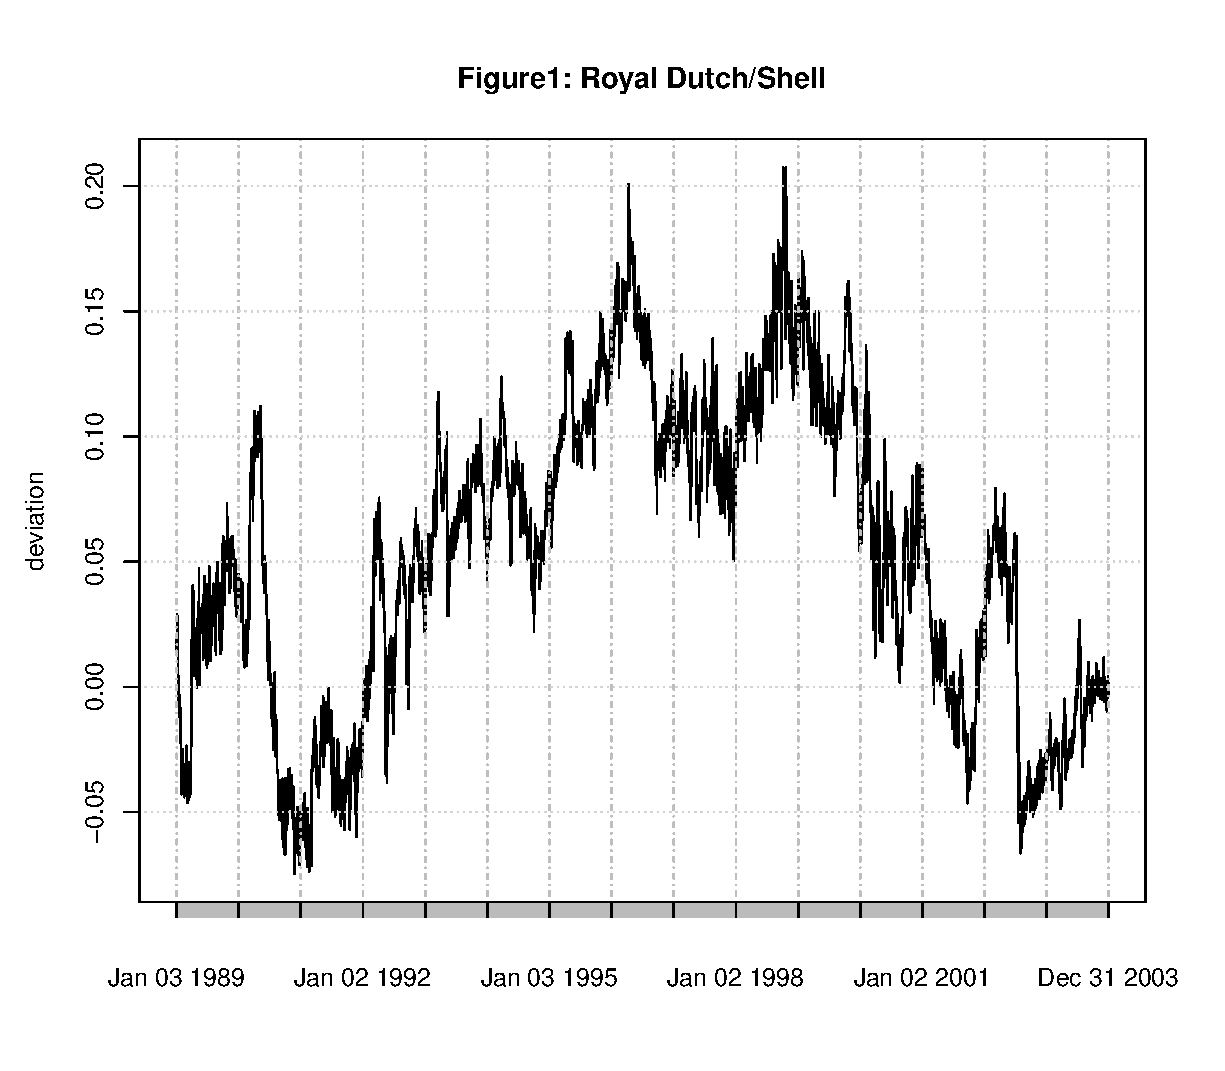
\includegraphics[width=\textwidth]{chapters/chapter_stat_ts/figures/471.eps}
	\caption{Royal Dutch/Shell. \label{fig:3royal}}
	\end{figure}
	
	\begin{figure}[!ht]
	\centering
	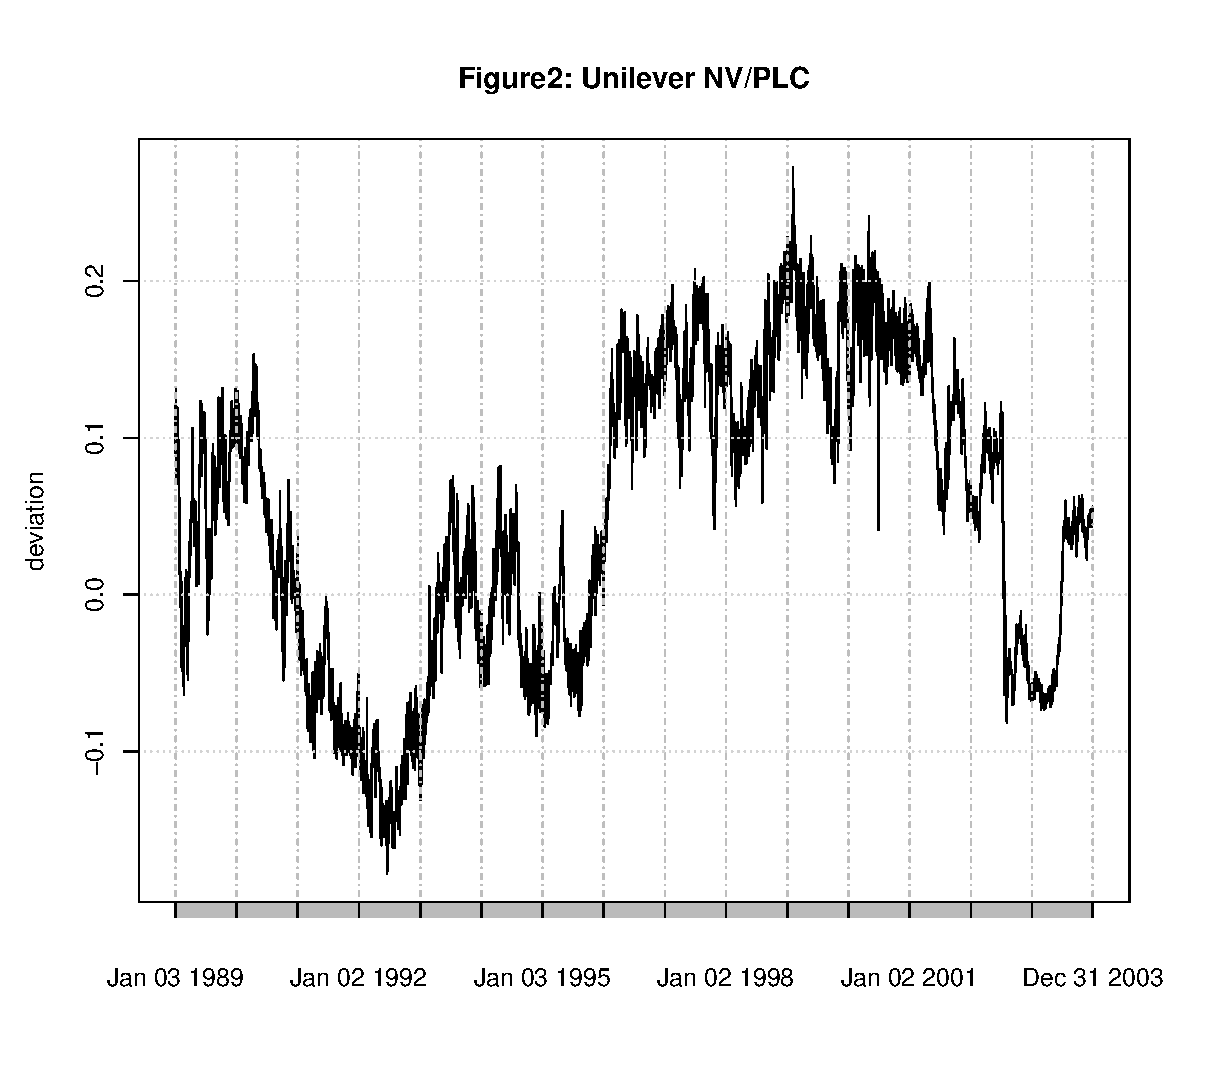
\includegraphics[width=\textwidth]{chapters/chapter_stat_ts/figures/472.eps}
	\caption{Royal Dutch/Shell. \label{fig:3nvplc}}
	\end{figure}

The first step in developing a pairs trading strategy is selecting two or more stocks that are closer to each other. The two example discussed here are natural-twins as their parent companies are the same. Generally mature companies with long trading histories and that have similar exposure to macro factors are considered for forming pairs; usually they tend to be from the same industry. We will discuss in detail how pairs can be formed later. First we present some formal procedures for implementing the pairs trading strategy.


\subsection{Distance-Based Algorithms}


Gatev, Goetzmann and Rouwenhorst (2006)~\cite{ggr} suggest using the distance based algorithm on normalized prices to identify the periods when the prices diverge. The normalization factor is a cumulative total returns index of the stock over the pairs formation period. Pairs are formed by computing the Euclidean distance between any two stocks and by selecting the pairs that are closer. A simple pairs trading algorithm is stated below, as illustration: \\

\noindent\fbox{%
    \parbox{\textwidth}{%
\noindent Pairs Trading Algorithm:
\begin{itemize}
\item Normalize the prices of every stock to equal unity, at the end of each calendar month, m; use the preceding 12 months as the estimation period; let $T_m$ be the number of trading days in the 12-month estimation associated with month $m$.

\item For each $t = 1,\ldots,T_m, p_t^i = \prod_{T=1}^t[1\times(1+r_T^i)]$, where $T$ is the index for all the trading days till $t$;

\item $\text{PD}_{i,j,m} = \sum_{i=1}^{T_m} \dfrac{p_t^i - p_t^j)}{T_m}$ \hfill \break 
$\text{St.Dev PD}_{i,j,m} = \sqrt{\dfrac{1}{T_m - 1}\sum_{i=1}^{T_m}[(p_t^i - p_t^j)^2 - \text{PD}_{i,j,m}]^2}$

\item If price difference (PD) diverges by more than 2 St.Dev PD, buy the cheaper stock and sell the expensive one; if pairs converge at later time, we unwind; if the pairs diverge but does not converge in 6 months, close the position.
\end{itemize}
        }%
} \\

Gatev et al (2006)~\cite{ggr} study the risk and return characteristics, using daily data from 1962 to 2002, of pairs trading for various sectors. The general finding is that pairs trading is profitable in every broad sector category. In relating the excess returns to the risk factors, market, SMB, HML, momentum and reversal, it is found that the exposures are not large enough to explain the average returns of pairs trading. Thus they conclude, ``\dots pairs trading is fundamentally different from simple contrarian strategies based on reversion.''


\subsection{Co-Integration}


There is some evidence that prices are co-integrated for the U.S. Stock market (see Bossaerts(1988)~\cite{bossaerts1988common}). If the price vector, $p_t$ is co-integrated with co-integrating rank, $r$ which imply that `$r$' linear combinations of $p_t$ are weakly dependent; thus these assets can be taken as somewhat redundant and any deviation of their price from the linear combination of the other assets prices is temporary and can be expected to revert. Writing the pairs trading concept in a model form has several advantages. It allows us to extend pairs to triplets etc and also can accommodate incorporating other factors such as other relevant indices.


A model based co-integration approach to pairs trading is elegantly presented in Tsay (2010, Section 8-8)~\cite{tsay}. It is based on the assumption that prices follow a random walk and on the additional expectation that if two stocks have similar risk factors, they should have similar returns; writing $p_{it} = \ln{(p_{it})}$ and with $p_{it}$ following a random walk, $p_{it} = p_{it-1} + r_{it}$ where $r_{it}$ is the return. Thus price series are said to be cointegrated, if there exists a linear combination, $w_t = p_{1t} - \gamma p_{2t}$ which is stationary and therefore mean reverting.


With the error correlation form of the bivariate series (follows from equation (90) in Ch 2),
	\begin{equation}
	\begin{bmatrix}
	p_{1t} - p_{1t-1} \\
	p_{2t} - p_{2t-1}
	\end{bmatrix}\quad
	= \begin{bmatrix} 
	\alpha_1\\ \alpha_2 
	\end{bmatrix}\quad 
	\begin{bmatrix} 
	w_{t-1} - \mu_{w}
	\end{bmatrix}\quad + 
	\begin{bmatrix} 
	a_{1t} \\ a_{2t} 
	\end{bmatrix}\quad
	\end{equation}
where $\mu_w = E(w_t)$ is the mean of $w_t$, which is the spread between the two log prices. The quantity $w_{t-1} - \mu_w$ denotes the deviation from equilibrium, $\alpha$'s show the effect of this past deviation on the current returns and should have opposite signs. Going long with one share of stock 1 and shorting $\gamma$ shares of stock 2, will result in the return of the portfolio, $\gamma_{p,t+i} = w_{t+i} - w_t$, at time `t'. The increment does not depend on $\mu_w$.


Based on the above discussion the following strategy can be followed. Let $\eta$ be the trading cost and $\Delta$ be the target deviation of $w_t$ from $\mu_w$ and assume $\eta < 2\Delta$.
\begin{itemize}
\item Buy a share of stock 1 and $\gamma$ shares of stock 2 at time t if $w_t = \mu_w - \Delta$

\item Unwind at time `$t+i$' $(i>0)$ if $w_{t+i} = \mu_w + \Delta$
\end{itemize}
Thus the return of the portfolio would be $2\Delta$ which is greater than the trading cost. For other modified versions of the strategy refer to Tsay (2010, Section 8.8)~\cite{tsay}.

From a practitioner standpoint, for testing if there is a co-integrating relationship between pairs, it is easier to use the two-step test proposed by Engle and Granger (1987)~\cite{engle1987co}
\begin{enumerate}[a)]
\item Run a regression model: $p_{1t}=\alpha+\beta p_{at} + u_t$

\item Test if the errors, $u_t$ are stationary, via the model $u_t=\gamma+\phi \mu_{t-1}+a_t$, with the null hypothesis $\text{H}_0: \phi=1$ vs  the alternative hypothesis $\text{H}_a: \phi<1$.
\end{enumerate}
If $u_t$ is stationary, it would imply the two prices $p_{1t}$ and $p_{2t}$ are co-integrated.


To illustrate pairs trading in real time, we consider the daily exchange rates between Indian rupee and U.S. dollar, GBP and Euro from December 4, 2006 to November 5, 2010. We normalize the first day's observation as unity and also note that the initial ratio is 1:1.98:1.33 in rupees for U.S. dollar, GBP and Euro respectively. From their plots in Figure~\ref{fig:rupee}, it is obvious that all three series move together until the middle of 2007, then the Euro takes off and then the U.S. dollar which is closely aligned with GBP takes off to join the Euro. For testing co-integration, one has to look at the three regimes individually. Thus tracking the co-integrating relationships over time, traders can generate profits by properly exchanging currencies.


	\begin{figure}[!ht]
	\centering
	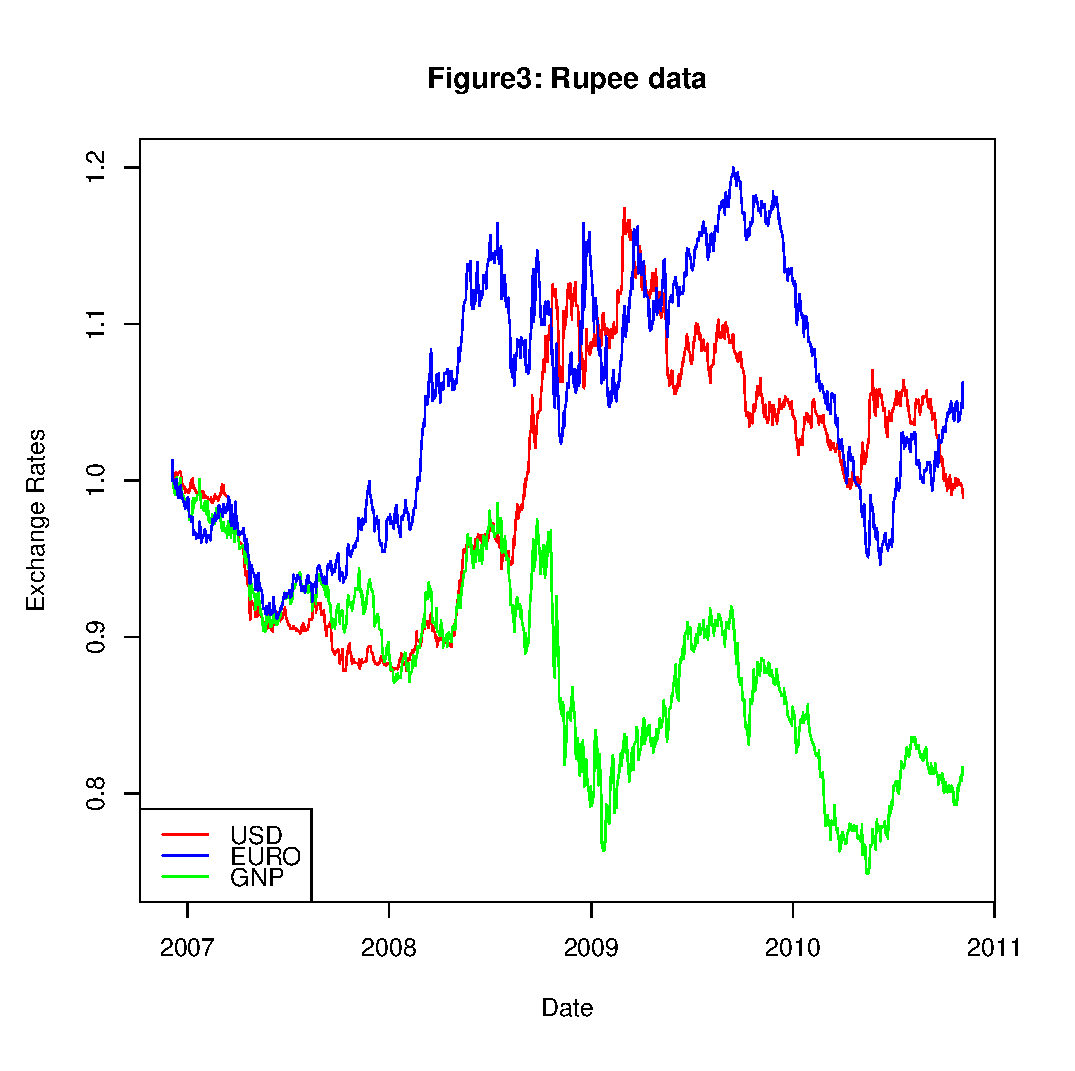
\includegraphics[width=\textwidth]{chapters/chapter_stat_ts/figures/473.eps}
	\caption{Rupee data. \label{fig:rupee}}
	\end{figure}

	\begin{figure}[!ht]
	\centering
	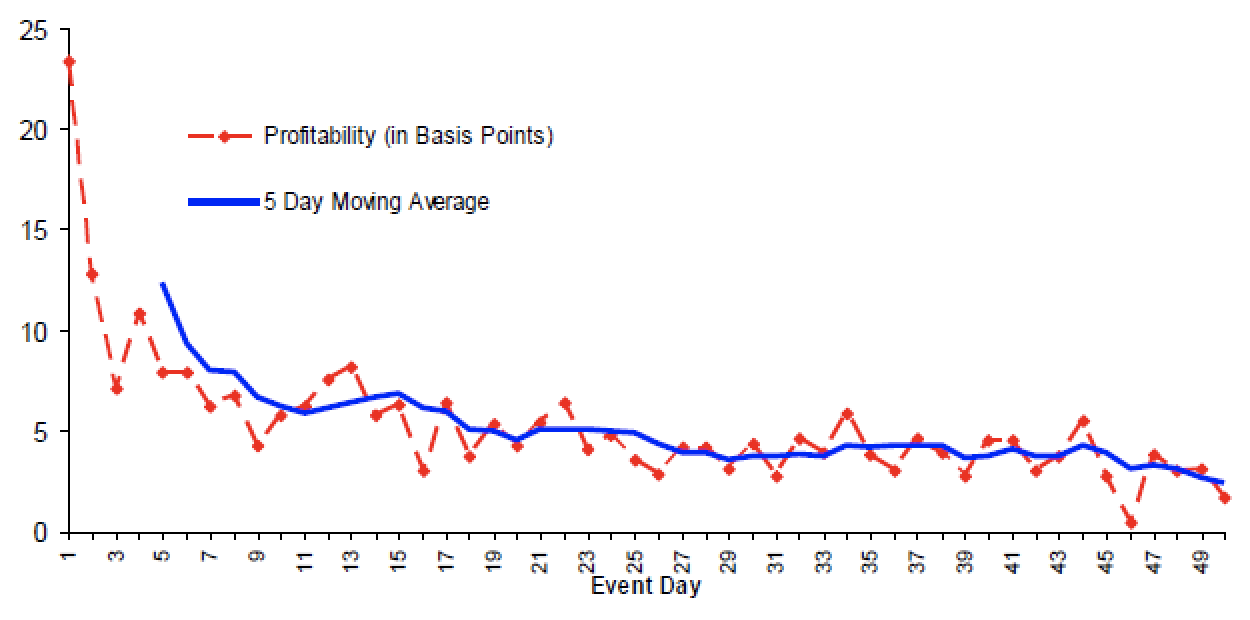
\includegraphics[width=\textwidth]{chapters/chapter_stat_ts/figures/Sec4-7Fig4.png}
	\caption{Pairs Trading Profitability in Event Time. \label{fig:pairsprofit}}
	\end{figure}


\subsection{Some General Comments}


\noindent\textbf{Finding Pairs:} An alternative approach is to use fundamentals of the firms to select two stocks that have similar risk factor exposures. Based on Asset Pricing Theory (APT) model,
	\begin{equation}
	r_{it} - r_{ft} = \alpha_i + \beta'_if_t + a_{it}
	\end{equation}
where $r_{ft}$ is the risk-free rate and $f_t$ are the factor scores. Now collect the coefficient vector $\hat{\theta}_i' = (\hat{\alpha}_i, \hat{\beta}_i)'$ for $i = 1,2,\ldots,N$ assets under consideration and form a standardized distance measure,
	\begin{equation}
	d_{ij}^2 = \hat{\theta}_i' \Cov^{-1}(\hat{\theta}_i)\hat{\theta}_i
	\end{equation}
and select pairs with the smaller distance. This hopefully will result in similar assets after adjusting for the risk factors. Generally the factors tend to vary much more slowly than the excess returns, $r_{it} - r_{ft}$, the distance based on $\hat{\theta}_i$ tends to move slower than short-term price movements. Recent studies confirm that the simple Euclidean distance-based pairing may be inadequate. Do and Faff (2010)~\cite{do2010does} suggest adding two additional metrics: industry homogeneity and the frequency of the historical reversal in the price spread; the measure in (\ref{eqn:et}) can accommodate that easily. \\

\noindent\textbf{High-Frequency Equity Pairs Trading:} While there is evidence of the profitability of pairs trading strategies at lower frequencies, not much is known in academia (but quite known in practice) about high-frequency intra-day pairs trading. Bowen, Hutchinson and O'Sullivan (2010)~\cite{bho} consider data from the London Stock Exchange for the most liquid stocks, the constituents of the index FTSE100. The duration is divided into a formation period, that is used to identify pairs of stocks that move together, and a trading period when the actual transactions occur. The distance based criteria using normalized prices is used to identify the top pairs during the formation period. As any other strategy, pairs trading profits are affected by transaction costs, and this becomes more acute as trading frequency increases. Results appear to be also quite sensitive to the speed of execution, as excess returns disappear quickly if execute delay is greater than one period. The majority of profits seem to occur in the first and last hour of trading, when relatively larger volatility and liquidity are occurring.


Although pairs trading has been used extensively by traders, it also has its limits. In a recent study, Engelberg, Gao, Jagannathan (2009)~\cite{engelberg2009anatomy} demonstrate that the opportunities for medium frequency pairs trading are not many and profits opportunities might vanish within a few days (see Figure~\ref{fig:pairsprofit}). Scruggs (2007)~\cite{scruggs} attributes the demise of Long-Term Capital Management to the hedge fund overconfidence in the strategy and their undue bets sizes compared to other market participants.


\subsection{Practical Considerations}


After identifying a potential pairs strategy via co-integration testing for instance, traders need to pay particular attention to the expected profitability of the strategy once real-life trading frictions have been taken into consideration. In practice, a significant portion of potential pairs trading strategies experience negative P\&L in production due to large execution slippage, whether originating from aggressive hedging at trade initiation, or position closing out.


When back testing a pairs strategy, one of the immediate cost that might render the strategy unprofitable is the spread cost. In other words, how much will it cost to extract liquidity when the signal triggers, in particular if the signal is too short-lived to allow for sourcing liquidity passively via limit order book posting. For intraday pairs trading it is also valuable to analyze if there is any asymmetry of cost between the initiation trade and the unwind trade. Often time, it is not uncommon to witness significantly higher exit costs once the market has normalized following a short-lived entry trade opportunity. 


The individual instruments microstructure also plays an important role in the strategy profitability. For instance long queue names  (instruments for which the top of book liquidity is large in comparison to daily volume)  are harder to trade because the time it takes for an order to reach the top of the queue and trade passively is generally larger than the time that is acceptable for the strategy to mitigate its legging risk\footnote{legging risk can be defined as the risk of not being able to fill timely a particular leg of a pair strategy at the required price}. As a result, most of the executions on the leg that displays a long queue will end up having to pay the full spread to be executed. 


As an example, when computing the spread ratio between two instruments using the market midpoint, one might be led to believe that the ratio is currently above $2\sigma$ of its distribution, warranting to initiate a trade. However, when considering the size of the spread and amount of the quoted volume on the passive side at the top of the book, it is not impossible that the realized ratio when crossing the spread is only a $0.5\sigma$ event, while getting a passive execution when quoting at the end of a long queue would represent a $5\sigma$ event that one shouldn't expect to realistically happen. These anecdotal examples give an idea of what practitioners should pay particular attention to when designing their strategies. Below, we mention a non-exhaustive list of implementation challenges also worth considering:

\begin{itemize}
\item \textbf{Difference in liquidity between the two legs}: Usually the selected pair has a slower moving leg and a faster moving one. This means that, in practice, one of the instruments might be ticking faster, thereby having a greater influence on the moves of the measured ratio. Additionally, faster ticking instruments also tend to have narrower spreads, meaning that in absence of control, the instrument the most likely to trigger a trade is also the one that is the cheapest to transact, forcing the strategy to then rapidly hedge out its exposure by paying the larger spread on the slowest ticking leg. One way of handling this situation is, for instance, to only let the strategy quote on the slow moving leg as long as it is ``in ratio'', and then only trigger the aggressive spread-crossing hedge trade if and when the passive leg receives a fill. 

\item \textbf{Rounding/tick size granularity}: While in theory it is possible to come up with a signal threshold that is as granular as desired, in practice the step increment of the signal might be constrained by the microstructure of the instruments traded. Most exchanges globally impose a minimum tick size increment that can vary based on the liquidity of the instrument. Here too, all things being equal, a practical approach would be to quote on the instrument which constrained tick size contributes the most to the ratio moves, and only trigger the aggressive spread-crossing hedge trade if and when the most constrained tick size leg receives a fill. 

\item \textbf{Signal stability}: As a result of both the difference in liquidity between long and short legs, and the potential frictions induced by the instruments microstructure described above, it is not uncommon for the signal to jump around the trigger ratio frequently. Trading in and out on each signal crossing of the pre-determined ratio would incur large transaction costs that would render many strategies unprofitable. To address this issue, a common approach is to define two different thresholds sufficiently apart for entering and exiting the trade so that signal noise does not trigger excess in and out trading. It's also possible to enforce a minimum holding duration to prevent the stop loss signal to trigger just due to local noise around the ratio threshold. 

\item \textbf{Time of day}: In the first 15 to 30 minutes after a market opens, many instruments have significantly wider bid-ask spreads while price discovery sets in after a night of information accumulation and no possible trading. If this significant difference in transaction costs is not properly accounted for, the trades initiated during that period can have an impact on the overall profitability of the strategy.

\item \textbf{Market asynchronicity}: While pairs are usually constructed between instruments trading concomitantly, it is also possible to construct pairs strategies with instruments from different markets. For instance, a pair between a US and a Japanese stock. This raises an additional challenge, which is: how to assess the theoretical value on an instrument that is not currently traded? Practitioners commonly address this issue by first modeling the relationship between the instruments daily time series, and then inferring its stability at more granular frequencies. The common risk can be hedged with a market wide instrument such as an index future, and be unwound overnight when the second leg is entered, thereby limiting unwanted exposure to market risk.

\item \textbf{Traditional Index Arb / ETF Arb}: When trading a pairs strategy between a composite instrument (Index, ETF, \dots) and its constituents, the fast and efficient nature of electronic markets might render trading opportunities too small to be exploited profitably across all instruments. In particular if the number of constituents is quite large, obtaining passive fills on most of them within a reasonable timeframe is not a realistic assumption. As a result, traders can implement partial replication strategies whereby they only trade an optimized tracking basket of the instruments that allow for the best replication under some liquidity and cost assumptions (spread size, top of book size, \dots). 

\item \textbf{Local market idiosyncrasies}: For instance, in Japan, sector classification (which is often used as a starting point for pairs selection or as a way to avoid picking names that would have spurious autocorrelation) does not match international sector classification one-for-one. Local market participants rely on the 33 TOPIX sectors that have a closer fit to the actual structure of the Japanese economy than the commonly used 11 GICS (r) sectors.

\item \textbf{Coupling market making and pairs trading strategies}: One possible approach to long queue and wide spread instruments pairs trading is to use a market making strategy to first gain queue priority in the longest queue name and achieve a certain child order density in the order book at regular volume-time intervals. For example, if only one of the instruments has a long queue, as long as the pairs strategy ratio is below the trigger threshold, the market making strategy can earn the spread on the long queue instrument while staying out of the market on the other instrument. When the ratio reaches the threshold, one can cancel the child orders created on the opposite side of the book by the market making strategy and only keep the ones on the side relevant to the pairs strategy. These orders, placed over time while market making, should already have accrued some queue priority, which will increase the probability of receiving a passive fill once the ratio is favorable. Then, the pairs strategy is able to trade aggressively the liquid leg as soon as the passive fill is received. Based on the liquidity and microstructure of the instruments in the pairs strategy, different equivalent strategies can be combined to achieve higher profitability.
\end{itemize}


\section{Cross-Sectional Momentum Strategies}


The trading strategies discussed thus far depend exclusively on the existence of time-series patterns in returns or on the relationships between returns and the risk factors. Time series strategies generally exploit the fact that stock prices may not follow random walks, at least in the short run. Even if prices follow random walks, it has been shown that strategies based on past performance contain a cross-sectional component that can be favorably exploited. For instance, momentum strategies demonstrate that the repeated purchase of past winners from the proceeds of the sale of losers can result in profits. This is equivalent to buying securities that have high average returns at the expense of securities that yield low returns on average. Therefore if there is some cross-sectional variance in the mean returns of the securities in the universe, a momentum strategy is profitable. On the other hand, a contrarian strategy will not be profitable even when the prices follow random walks. For the demonstration of the rules of the momentum strategy in the low frequency setting, refer to Jegadeesh and Titman (1993)~\cite{JeTit1993}, 2002~\cite{JeTit}) and Conrad and Kaul (1998)~\cite{conrad1998}.


To better understand the sources of profit from a momentum strategy Lo and MacKinlay (1990)~\cite{lo1990} decompose the profit function into three components. We will follow the set-up as presented in Lewellen (2002)~\cite{lew2002}. Let $r_{i,t-1}^k$ be the asset $i$'s, `$k$' month return ending in `$t-1$' and let $r_{m,t-1}^k$ be the return from the equal-weighted index's `$k$' month return ending in `$t-1$'. The allocation scheme over `$N$' assets under the momentum strategy is,
	\begin{equation}
	w_{i,t}^k= \frac{1}{N} (r_{i,t-1}^k - r_{m,t-1}^k)
	\end{equation}
For ease of interpretation, $w_{i,t}^k = w_{i,t}$ and focus on only one previous month's return for allocation; let $r_t$ be a $N \times 1$ vector of returns, with the mean return $\mu = E(r_t)$ and $\Omega = E[(r_{t-1} - \mu)(r_t - \mu)']$ the autocovariance matrix of returns. Let $w_t$ be $N \times 1$ vector of weights, $w_{it}$; the portfolio return for month `t' is $\pi_t = w_t'r_t$. It is easy to show
	\begin{equation}
	\begin{split}
	E(\pi_t)&= \frac{1}{N}\, E\left[\sum_i r_{i,t-1} \cdot r_{it} \right] - \frac{1}{N} E\left[r_{m,t-1} \cdot \sum_i r_{it} \right] \\
	&= \frac{1}{N}\sum_i (\rho_i + \mu_i^2) - (\rho_m + \mu_m^2)
	\end{split}
	\end{equation}
where $\rho_i$ and $\rho_m$ are lag 1 autocovariance of asset `$i$' and the equal weighted index. Note that the average autocovariance is $\text{tr}(\Omega)/N$ and the autocovariance for the market as a whole is $(1' \Omega 1)/N^2$. The $\text{tr}(\Omega)$ denotes the sum of the diagonal elements of $N \times N$ matrix $\Omega$; recall that the diagonal elements are the autocovariance, $\rho_i$, of individual stocks. Hence (\ref{eqn:}) can be written as,
	\begin{equation}\label{eqn:3epi}
	E(\pi_t) = \left(\frac{N-1}{N^2}\right)\cdot \text{tr}(\Omega) + \frac{1}{N^2} [\text{tr}(\Omega) - 1' \Omega 1] + \sigma_{\mu}^2
	\end{equation}
The three terms in (\ref{eqn:3epi}) precisely identify three sources why positive profits occur (see Lo and Mackinlay (1990)~\cite{lo1990}):
\begin{itemize}
\item Stock returns are positively autocorrelated, so each stock's past return predicts high future return,

\item Stock returns are negatively correlated with the lagged returns on other stocks, so their poor performance predicts high returns for others

\item Some stocks have simply high unconditional mean returns relative to other stocks.
\end{itemize}


The finance literature is replete with empirical verifications of the momentum strategy. However, the analytical decomposition in (\ref{eqn:}) is not informative about the economic sources of momentum. Why the momentum strategy works has been attributed to various theories. The literature argues that firm-specific returns drive momentum. Firm-specific returns can be persistent because investors under-react to firm-specific news or stock returns covary strongly due to a common influence of a macro factor. Lewellan (2002)~\cite{lew2002} shows that the Size and B/M portfolios also exhibit strong momentum; as these portfolios are well-diversified, their returns reflect systematic risk and therefore macroeconomic factors must be responsible for the momentum. Hvidkjaer (2006)~\cite{hvid2006} suggests that momentum could be partly driven by the behavior of small traders who under-react initially, followed by delayed reaction to buying and selling pressures. The trading pressure tend to translate into price pressures that affect the trading behavior of the small traders.


Although cross-sectional momentum is widely documented, among the three components in (27)(\ref{eqn:}), time series momentum as represented by the first term tends to dominate for every liquid instrument in a sample of 58 instruments spread over a variety of asset classes, equity index, currency, commodity and bond futures. Moskowitz, Ooi and Pedersen (2012)~\cite{mos2012} show that the autocovariance term, $\text{tr}(\Omega)/N$ is the dominant factor, particularly in foreign exchange and equity markets. To make meaningful comparison across asset classes, the excess returns are scaled by their ex-ante volatilities and the following models are estimated for predicting price continuation and reversal:
	\begin{equation}
	\frac{r_t^s}{\sigma_{t-1}^s} = \alpha + \beta_h \dfrac{r_{t-h}^s}{\sigma_{t-h-1}^s} + \varepsilon_t^s
	\end{equation}
and
	\begin{equation}
	\frac{r_t^s}{\sigma_{t-1}^s} = \alpha + \beta_h \sgn(r_{t-h}^s) + \varepsilon_t^s
	\end{equation}
where $h= 1,2,\ldots,60$ months and the ex-ante annualized variance $\sigma_t^2$ is calculated as follows:
	\begin{equation}
	\sigma_t^2 = 261 \sum_{i=0}^\infty (1-\delta)\,\delta^i \,(r_{t-i} - \overline{r}_t)^2
	\end{equation}
Here the weights $\delta^i (1 - \delta)$ add up to one, $\overline{r}_t$ is the exponentially weighted average return computed in a similar fashion. The exponential smoothing parameter is chosen to be $\sum(1-\delta)\delta^i = \frac{\delta}{1-\delta} = 60$ days. Using $\sigma_{t-1}$ in (\ref{eqn:}) and (\ref{eqn:}) avoids the look-ahead bias\footnote{WE PROBABLY NEED A FOOTNOTE HERE TO ENSURE THE READER UNDERSTANDS}.


We can also investigate the profitability of strategies based on time series momentum with varying look-back period ($k$) and holding period ($h$). If the excess return over the past k months is positive, go long or otherwise go short. The position size is taken to be, $1/\sigma_{t-1}^s$, inversely proportional to the ex-ante volatility of the instruments, `$s$'. With this choice it is argued that it will be easier to aggregate the outcome of the strategies across instruments with different volatilities and it will also lead to somewhat stable time series. For each trading strategy $(k,h)$, a single time series of returns, $r_t^{\text{TSMOM}(k,h)}$, which is the average return across all portfolios active at time, `$t$' is computed. To evaluate the overall value of the time series momentum strategies, the returns are adjusted for possible risk factors:
	\begin{equation}
	\begin{split}
	r_t^{\text{TSMOM}(k,h)}&= \alpha + \beta_1 \text{MKT}_t + \beta_2 \text{BOND}_t + \beta_3 \text{GSCI}_t + \beta_4 \text{SMB}_t \\
	&=  + \beta_5 \text{HML}_t + \beta_6 \text{UMD}_t + a_t 
	\end{split}
	\end{equation}
where $\text{MKT}_t$ is the excess return on the MSCI World index, $\text{BOND}_t$ is Barclay's Aggregate Bond Index, $\text{GSCI}_t$ is S\&P GSCI commodity index and the others are Fama-French factors for the size, value and cross-sectional momentum premiums.


Using monthly data spanning January 1985 to December 2009, Moskowitz et al (2012)~\cite{mos2012} find that the time series momentum strategies provide additional returns over and above a passive buy and hold strategy. They also show that the model (\ref{eqn:}) results in a large and significant alpha. The analysis also illustrates that speculators are likely to benefit from following trends at the expense of hedgers. The time series momentum appears to last about a year and then begins to reverse.


The momentum strategies remain profitable even after adjusting for price impact induced by trading. Although the trading decisions are done at a macro level, the actual trading takes place at a micro level. The price impact (see Chapter 8) is the impact of the current trade on the subsequent trades. Korajczyk and Sadka (2004)~\cite{kora2004} demonstrate that certain $(k,h)$ strategies are profitable if the proportional costs equal the effective and quoted spreads.


The role of trading volume in explaining the results of momentum strategies is studied in Lee and Swaminathan (2000)~\cite{lee2000}. They find that, in equilibrium, both price and volume are simultaneously determined. In addition to the decile classification based on the past returns, the universe of stocks was further divided into three volume size categories, yielding thirty groups. The study provides evidence that low volume stocks tend to be under-valued by the market. Thus investor expectations affect not only a stock return but also its trading volume. High volume firms generally earn lower future returns. The general notion that volume fuels momentum is not supported but is true for losers and ``it helps information ``diffusion'' only for winners.''


It is worth mentioning that while most documented applications of the momentum strategy are in equity markets, there is a growing academic interest in their use in foreign exchange (FX) markets. The FX markets were traditionally cited as markets where technical rules such as trend following have been successful. But studies such as Menkhoff, Sarno, Schemeling and Schrimpf (2012)~\cite{menkhoff2012} have explored the cross-sectional momentum and have demonstrated their profitability (up to 10\%) in FX markets. The momentum portfolios in FX markets are observed to be skewed toward minor currencies that have somewhat higher transaction costs. The base currency returns, $r_t= \ln(S_t) - \ln(S_{t-1})$ where $S_t$ is the spot exchange rate, and the interest-adjusted return, where $F_{t-1}$ is the future price at $t$-1,
	\begin{equation}
	\begin{split}
	r_t^* &= \ln(S_t) - \ln(F_{t-1}) \\
	&= \ln(S_t) - \ln(S_{t-1}) + \ln(S_{t-1}) - \ln(F_{t-1}) \\
	&\sim r_t + \dfrac{(r_f - r_d}{12}
	\end{split}
	\end{equation}
which is the sum of pure currency appreciations and the return due to interest rate appreciation. Here $r_f$ is the foreign interest rate and $r_d$ is the domestic interest rate; See Okunev and White (2003)~\cite{okunev2003} for the details of this decomposition. It is found that the profitability is clearly originating from spot rate changes themselves and not necessarily driven by the interest rate differential.


In the equity markets, it is argued that momentum strategies are successful because of slow information processing and investor overreaction. However FX markets are dominated by professionals and thus any information should be impounded in the FX rate almost instantaneously. But if the portfolios are mostly made up with minor currencies, they are likely to exhibit higher volatility, higher country risk and higher interest-rate changes, thus imposing effective limits to arbitrage. It is further observed that the cross-section based currency momentum is not related to benchmark technical trading strategies and even after adjusting for them, the cross-sectional momentum profits are found to be higher.


\section{Multiple Indicators and Boosting Methods}

x
In developing models that capture the main features of the data, it must be noted that there are no unique models. Thus they yield different forecasts. It is well-known in the forecasting literature that a combined forecast generally does perform better than the individual forecasts. If there are `$T$' models and thus `$T$' forecasts, $\hat{f}_1,\ldots, \hat{f}_T$, how do we combine them to get a single forecast? Because these are all based on the same data, the estimates are likely to be correlated, resulting in a covariance matrix, $\hat{\Sigma}_f$. Three estimates that are proposed in the literature are:
	\begin{table}[!ht]
	\caption{Three proposed estimates}
	   \begin{tabular}{l l r}
             \textbf{Weighted Estimator 1: \hskip 1mm}& $\hat{f}_{w_1}=\hat{f}' \hat{\Sigma}_f^{-1} \hat{f}$ & \pushright{\text{(??)}} \\
             \textbf{Weighted Estimator 2: \hskip 1mm}& $\hat{f}_{w_2} = \hat{f}' (\text{diag}\hat{\Sigma}_f)^{-1} \hat{f}$ & \pushright{\text{(??)}}\\
             \textbf{Simple Average Estimator: \hskip 1mm}& $\sum_{i=1}^T \frac{\hat{f}_i}{T}$ & \pushright{\text{(??)}} \\
	 \end{tabular}
	 \end{table}
Due to the uncertainty in the estimation of $\Sigma_f$ in regime changes that results in large estimation error, the simple average estimator is advocated. In the context of modeling the asset prices the elements of $\Sigma_f$ represent how well the methods do in forecasting. In order to use the above weighted estimators we need to keep track of the performance of the individual forecasting methods and in principle, the methods that yield inferior forecasts would get less attention. But a question about the span of their performance, recent versus past, remains open. \\


\noindent \textbf{Ensemble Learning} \\


As mentioned, the idea of combining multiple forecasts (classifiers) into a single one is a longstanding goal of many decision-makers. This is especially important when methods that are successful at different regimes are complementary. There are two types of ensemble methods, bagging and boosting that we discuss here. Suppose the goal is to determine if we want to enter the market or not based on the information available at that time. It is somewhat easier to come up with simple rules but is harder to find a rule that has high accuracy. Under boosting, we study how to combine the simple rules uniformly into a `stronger' rule. It is suggested to focus on examples that are hardest to forecast by simple rules and take a weighted majority of these rules to come up with a stronger rule.


To motivate, we will assume that we want to determine whether the price of an asset will go up or down. Under the random walk model, the error in guessing randomly is 0.5. But any rule should result in an error less than 0.5. We begin with a training set, $S=\{ (x_i,y_i), i=1,2,\ldots n\}$ where $x_i$ is the information and $y_i$ is a binary variable that indicates whether to enter the market or not. Assume that there are `$T$' rules, $h_t(x)$ are the classifiers and $D_t$ is the distribution over the training set with the error,
	\begin{equation}
	\text{err}_D(h)=Pr_{(x,y) \sim D}(h(x) \neq y) 
	\end{equation}
The rule $h_t$ is supposed to have error $\text{err}_{D_t}(h_t)$ with respect to `$D_t$'. \\

\noindent The boosting algorithm works as follows:


\begin{table*}[!ht]
   \begin{tabular}{l l r}
             \textbf{Initialize: \hskip 1mm}& $D_t(i)=\frac{1}{n} \text{ for all } `i' $  \\
             \textbf{Iterate: \hskip 1mm}& $D_{t+1}(i)=\frac{D_t(i)}{z_t} \cdot \text{exp}[-\alpha_t y_i h_t(x_i)]$ \\
             & \text{ when } $\alpha_t=\frac{1}{2}\text{ln}\left(\frac{1-\text{err}_{D_t}(h_t)}{\text{err}_{D_t}(h_t)}\right), z_t=\text{normalizing constant}$ & \pushright{\text{(??)}}\\
             \textbf{Stopping Time: \hskip 1mm}& $ \text{Stop when the error in (1) on a validation data set does not improve}$ \\
              \textbf{Final Rule: \hskip 1mm}&$ \text{Sign}(\sum_{t=1}^T \alpha_t h_t(x)) $\\
 \end{tabular}
 \end{table*}
 
 
 It is possible that overfitting can happen with boosting; its performance clearly depends upon how well the two decisions (enter or not enter) are clearly separated based on the past data. The use of kernels can improve local separability. It is also important to optimally extract features, $x$, that can be discriminating between the two options for $y$. The main advantage of ensembles of different rules is that it is not likely that all rules will make the same error. The algorithm described in (33) and (34) is known as, ``adaptive boosting algorithm (AdBoost)'' is by Freund and Schapire (1995, 1996,1997)~\cite{freund1995decision}~\cite{freund1996experiments}~\cite{freund1997decision} and it automatically ``adapts'' to the data at hand. If $t^{th}$ classifier $h_t(x)$ is parameterized and the overall predictor takes the form,
	\begin{equation}
	h(x)=\text{Sign}\left(\sum_{t=1}^T \alpha_t \text{Sign}(w^{(t)}x+b^{(t)} \right)
	\end{equation}
is a two-layer neural network with `$T$' hidden units. One can see the identical underlying nature of the structure between neural network and boosting algorithm.


The idea of bagging comes from training the rules on multiple data sets that supposedly have similar structure. The multiple data sets are obtained by bootstrap  resampling. The bootstrap data sets are not likely to be too similar. For the data on asset prices, which are represented by an AR(1) model with the coefficient close to one, the asymptotic distribution of the sample estimate of the coefficient is non-normal. So the bootstrap samples are also useful to construct the appropriate sampling variance. The bootstrap samples are created by resampling the innovations or empirical residuals. From the single data set, $S$ we create `$M$' bootstrapped samples, $S_1,\ldots, S_M$ with each set containing `$n$' samples. Then apply the boosting method on all these samples and average them. As noted in the literature, bagging tends to reduce variance and thus it provides an alternative to regularization, see Breiman (1996)~\cite{breiman1996bagging}.


The gradient boosting method introduced by Breiman (1999)~\cite{breiman1999prediction} and generalized by Friedman et al. (2000)~\cite{friedman2000additive} and Friedman (2001)~\cite{friedman2001greedy} further improves on the ADA boost. The method starts by fitting an additive model (ensemble), $\sum_t \alpha_t h_t (x)$ in a forward stage-wise manner. In each stage, a weak learner is introduced to compensate for the shortcomings of existing weak learners. In gradient boosting, gradients are used to identify the shortcomings and in the regression context, these are residuals. Now the training set, $S^*=\{(x_i, y_i-h(x_i)) , i =1,\ldots,n\}$ is treated like, $S$, with residuals playing the role of the data. The optimization occurs by moving in the opposite direction of the gradient of the function.


\section{Evaluation of Strategies: Various Measures}


It is important to develop measures to evaluate the trading strategies. The standard measures stem from the capital asset pricing model:
	\begin{equation}
	r_{t} - r_f = \alpha + \beta (r_{mt} - r_f) + \varepsilon_{t} 
	\end{equation}
where $r_t$ is the return on the asset and $r_f$ is the return from a risk-free asset; the slope coefficient, $\beta$ measures the riskiness of the asset and $'\alpha'$ denotes the excess return. Thus a strategy can be simply evaluated by: \\


\noindent\textbf{Excess return: }$\alpha$ with positive values of `$\alpha$' indicating better performance. \\

\noindent More popular measures are:\\

\noindent \textbf{Sharpe Ratio: } $\dfrac{E(r_{t}) - r_f}{\sigma}$: Standardized by the volatility of the asset. \\

\noindent \textbf{Treynor Ratio: } $\dfrac{E(r_{t}) - r_f}{\left|\beta \right|}$: Standardized by market risk. \\

\noindent with appropriate sample estimates substituted here. A modified version of excess return is known as,

\noindent \textbf{Information Ratio: } $\dfrac{\alpha}{\sigma(\varepsilon_{t})}$: Standardized $\alpha$

While the above ratios take a long-term view of the investments, two others that are used in industry focus on the execution aspects of the strategies: \\

\noindent \textbf{Sortino Ratio: } $\dfrac{E(r_{t}) - r_{\text{target}}}{DR(r_{t})}$, \\

\noindent where $r_{\text{target}}$ is the target rate chosen by the investor and DR($r_t$) denotes the downside volatility or the draw down. Another measure is, \\

\noindent \textbf{Calmar Ratio: } $\dfrac{\text{Compound Annualized Rate of Return}}{\left| \text{ Maximum Drawdown }\right|}$ \\


The attention to drawdown is important because there is no guarantee that a strategy chosen through simple back-testing will work in the future. The last two ratios combine both the idea of maximizing the return and the idea of minimizing the loss. The drawdown numbers are essentially determined by the traders based on their own experience and their risk tolerance. There are some studies that focus on the statistical properties of their criteria (see Bertrand and Protopopescu (2010)~\cite{bertrand} on the information ratio and A. Lo (2002)~\cite{awlo} on the Sharpe ratio). Another measure is to simply compare the strategy's returns to the returns from buy and hold.


The standard reporting of backtesting results include, number of winning and losing trades, largest winning and losing trades, net slippage, total commissions along with annualized versions of the above ratios. 


\section{Extraneous Signals: Trading Volume, Volatility, etc.}


The trading algorithms that are presented in this chapter thus far focus on the price and return behavior of an equity. In pairs trading, we considered the behavior of price-return of a related equity to decide when to buy one and sell the other. But there is information as noted in Section 2.7 from the volume of trading. The model discussed there relates the volume to volatility. If there is no variation in the information flow about an equity, there should not be any correlation between volume traded and the return volatility. If the correlation exists we could indirectly infer that there is information and we may want to exploit that for trading. There is a vast literature in finance studying the relationship between trading volume and serial correlation in returns. We briefly review some select studies and provide an illustrative example with some possible algorithms. 


Blume, Easley and O'Hara (1994)~\cite{blumeohar} investigate the informational role of volume. If the impounding of information into stock price is not immediate, volume may provide information about the evolving process of security returns. The model discussed in Section 2.7 by Tauchen and Pitts (1983)~\cite{tauchenpitts} and the associated empirical tests clearly document strong relationship between volume and the absolute return. `But why such a pattern exists or even how volume evolves in markets is not clear.' Recall that the model assumes that the information content affects both the return and the volume specifications; yet the correlation between the return and volume can be shown to zero. If the information content can be studied through the sequence of security prices and the associated volume, if may provide insights into the inefficiency in the market and how statistical arbitrage rules can exploit it especially if there is a lead-lag relationship. The quality of trader's information can be captured best by combining price change with volume change. It is shown that the relationship between volume and price is in the form of V-shape thus indicating a non-linear relationship. Both `bad' and `good' information about the stock will result in higher volume of trade. 


Campbell, Grossman and Wang (1993)~\cite{campbellgross} also explore the relationship between volume and returns; volume information is used to distinguish between price movements that occur due to publicly available information and those that reflect changes in expected returns. It is predicted that price changes with high volume tend to be reversed and this may not happen on days with low volume. Llorente, Michaely, Saar and Wang (2002)~\cite{llmsw} extend this work by postulating that the market consists of liquidity and speculative traders. In periods of high volume but speculative trade, return autocorrelation tends to be positive and if it is liquidity trading return autocorrelation tends to be negative. In the former case, returns are less likely to become reverse. Defining the turnover ($V$) as the ratio of number of shares traded to the total number of outstanding shares, the following regression model is fit for each stock:
	\begin{equation}\label{eqn:regxt}
	r_t= \beta_0 + \beta_1 r_{t-1} + \beta_2 V_{t-1} \cdot r_{t-1} + a_t
	\end{equation}
For stocks associated with more speculative trading (larger bid-ask spreads), $\beta_2$ is expected to be positive. The model can be extended to add a market proxy ($r_{mt}$). Note the first order autocorrelation that we expect to hold different signs under different volume-return scenario are captured by `$\beta_1$' coefficient. The model's predictions are tested for NYSE and AMEX stocks and the results are supportive of the predictions. 


Gervais, Kaniel and Mingelgrin (2001)~\cite{germing} show that stocks with unusually large trading activity over periods tends to experience large returns over the subsequent periods. It is argued that higher trading activity creates higher visibility and in turn creates subsequent demand for that stock. This approach where contrarian or momentum is characterized by trend in volume is also studied by Conrad, Hameed and Niden (1994)~\cite{conniden} and Lee and Swaminathan (2000)~\cite{lee2000}. Assume that the change in trading activity is measured by
	\begin{equation}\label{eqn:uit3}
	u_{it}=(V_{it} - V_{it-1})/V_{it-1}
	\end{equation}   
and a positive $u_{it}$ implies higher transaction security and a negative $u_{it}$ is taken to imply low transaction security. Form four portfolios with stocks that exhibit positive versus negative returns in conjunction with positive versus negative transaction activity. The weight for each of the form portfolios are given as:
	\begin{equation}\label{eqn:wip3}
	w^*_{i,t} = \dfrac{r_{it-1}(1+u_{it-1})}{\sum_{i=1}^{N_p} r_{it-1}(1+u_{it-1})}
	\end{equation}
where $N_p$ is the number of securities in each combination ($p=1,\ldots,4$). The empirical results confirm that autocorrelation of low and high transaction securities are different; high transaction stocks experience price reversals and low transaction stocks experience positive autocorrelations in returns. These relationships are noted to be stronger for smaller firms. 


The discussion thus far refers to the use of low frequency data. Most of the studies deal with daily or weekly data that are aggregated. Simply using the end of the period closing price and the volume for the period is not appropriate as transactions occur at specified prices. The availability of high-frequency data has enabled to study the evolving influence of volume after controlling for order book imbalances. Because the parent order gets sliced into small child orders, both the number of trades and size of trades need to be considered in the place of volume. As argued in Kyle (1985)~\cite{kyle1985}, the price volatility is induced by net order flow. Market makers tend to infer information from the net order flow and revise their prices. Using a random sample of approximately three hundred stocks in NYSE, Chan and Fong (2000)~\cite{chanfong} consider the model in two steps for daily data: 
	\begin{equation}\label{eqn:riteit}
	\begin{split}
	r_{it} &= \sum_{k=1}^4 d_{ik} D_{kt} + \sum_{j=1}^{12} \beta_{ij} r_{it-j} + \epsilon_{it} \\
	\epsilon_{it} &= \phi_{i_0} + \phi_{im} M_t + \sum_{j=1}^{12} \phi_{ij} |\epsilon_{it-j}| + \gamma_i (V_i \text{ or }T_i) + \eta_{it}
	\end{split}
	\end{equation}
Here $D$ is the day-of-the week indicator, $M_t$ is an indicator for Monday, $V$ and $T$ are share volume and number of trades. The second equation that measures the volume-volatility relationship indicates that the number of trades ($T$) has a better explanatory power than share volume ($V$). The relationship between order book imbalance and volatility is captured by modifying the first equation in (\ref{eqn:riteit}) as
	\begin{equation}\label{eqn:rit32}
	r_{it}=\sum_{k=1}^5 \alpha_{ik} D_{kt} + \sum_{j=1}^{12} \beta_{ij} r_{it-j} + \sum_{h=1}^5 \lambda_{h,i} N T_{h\cdot it} + \Eulerconst_{it}
	\end{equation}
where $NT_{h,it}$ is the net number of trades in size category `$h$'. The net number is calculated by classifying the trade as buyer-initiated or seller-initiated using Lee and Ready (1992)~\cite{leeready} rule. It is shown that the coefficient `$\lambda$' is positive and significant for most stocks. But the second-stage regression results in weaker `$\gamma$' values. 


Chordia, Roll and Subrahmanyam (2002)~\cite{chorroll} extend this and provide a more comprehensive empirical analysis; resulting stylized facts are listed below:
	\begin{enumerate}[--]
	\item Order imbalances are strongly related to market returns; imbalances are high after market declines and low after market advances.
	\item Liquidity is not predictable from past imbalances but is predictable from market returns.
	\item Order imbalances are strongly related to volatility measures after controlling for volume and liquidity. 
	\end{enumerate}
These stylized facts would be useful for spotting anomalies and hence for devising appropriate trading strategies. 


\subsection{Filter Rules based on return and volume}


The rules that were discussed in Section 3.2 can all be modified to include volume as a weighing factor for the returns. That would involve tracking both the price and volume changes over time; it gets particularly cumbersome to track the volume that is appropriately normalized for the time of the day. Therefore the rules focus on defining and tracking the changes in the two quantities individually and combine them with necessary thresholds. Cooper (1999)~\cite{cooper} suggests four strategies based on weekly returns and another four strategies that incorporate the return (thus price) and the volume information. First the return rules are for weeks `$t-1$' and `$t-2$': \\

\noindent First-Order Price Filters: \\ 
\begin{equation*}\label{eqn:firstorder} 
	\textrm{Return states} = \left\{ 
		\begin{array}{ll}
	\!\!\!\!\textrm{For} ~k = 0,1,\ldots,4:& \!\!\!\! \left\{ 
		\begin{array}{ll}\textrm{loser}_{k^\star A} & \!\!\!\! \textrm{if}~ -k^\star A>r_{i,t-1}\geq - (k+1)^\star A \\
		 \textrm{winner}_{k^\star A}&\!\!\!\!\textrm{if}~ k^\star A\leq r_{i,t-1} <  (k+1)^\star A
		 \end{array} \right.\\
	\!\!\!\!\textrm{For}~ k = 5:& \!\!\!\!\left\{ 
		 \begin{array}{ll}\textrm{loser}_{k^\star A} & \!\!\!\!\textrm{if}~ r_{i,t-1} <-k^\star A \\ 
		 \textrm{winner}_{k^\star A} & \!\!\!\!\textrm{if}~  r_{i,t-1} \geq  k^\star A
		 \end{array}\right.
		\end{array} 
		\right. 
	\end{equation*} \\ 
\noindent Second-Order Price Filters: \\ 
	\begin{equation}\label{eqn:secondorder} 
\scalebox{0.85}{$
	\textrm{Return states} =\left\{ 
		\begin{array}{ll}
		\!\!\!\!\textrm{For} ~k = 0,1,\ldots,4: & \!\!\!\! \left\{ 
			\begin{array}{ll}
			\textrm{loser}_{k^\star A} & \!\!\!\!\textrm{if}~ -k^\star A>r_{i,t-1}\geq - (k+1)^\star A \\ 
			\textrm{     and} & -k^\star A > r_{i,t-2} \geq -(k+1)^\star A \\
			\textrm{winner}_{k^\star A} & \!\!\!\!\textrm{if} ~k^\star A\leq r_{i,t-1} <  (k+1)^\star A \\ 
			\textrm{     and} & k^\star A \leq r_{i,t-2} < (k+1)^\star A
			\end{array}\right.\\
		\!\!\!\!\textrm{For} ~k = 5:& \!\!\!\!\left\{ 
		\begin{array}{ll}
		\textrm{loser}_{k^\star A} & \!\!\!\!\textrm{if}~ r_{i,t-1} <-k^\star A \\ 
		\textrm{     and}  & r_{i,t-2} <-k^\star A \\
		\textrm{winner}_{k^\star A} & \!\!\!\!\textrm{if}~  r_{i,t-1} \geq  k^\star A \\ 
		\textrm{     and} & r_{i,t-2} \geq k^\star A 
		\end{array}\right.
\end{array} \right. $}
	\end{equation} 
Here $r_{i,t}$ is the non-market-adjusted return for security `$i$' in week `$t$',  $k$ is the filter counter, $k=0,1,2,\ldots,5$ and $A$ is the lagged return gird width,  set equal to 2\%. 


To relate if return reversals are related to trading volume, define the growth volume as the percentage changes in volume adjusted for the outstanding shares: 
	\begin{equation}\label{eqn:perdeltav}
	\%\Delta v_{i,t} = \left[\frac{V_{i,t}}{S_{i,t}}-\frac{V_{i,t-1}}{S_{i,t-1}}\right] / \left[\frac{V_{i,t-1}}{S_{i,t-1}}\right]
	\end{equation}
Here $S_{i,t}$ is the number of outstanding shares. Next, we define filters based on this: \\


\noindent Volume Filters: 
	\begin{equation}\label{eqn:volfilter}
	\scalebox{0.89}{$\textrm{\small Growth in volume states} = \left\{ 
	\begin{array}{lllll}
		\!\!\!\!\textrm{For} ~k = 0,1,\ldots,4: & \!\!\!\!\left\{ 
			\begin{array}{lllll}
			\!\!\!\! \textrm{low}_{k^\star B}\;  \textrm{if } -k^\star B &\!\!\!\!>\!\!\!\! & \!\!\!\! \%\Delta v_{i,t-1} \\
			\!\!\!\!& \!\!\!\!\geq & \!\!\!\!- (k+1)^\star B \\
	\!\!\!\! \textrm{high}_{k^\star C}\; \textrm{if } k^\star C & \!\!\!\!\leq&\!\!\!\! \%\Delta v_{i,t-1} \\
	&\!\!\!\!<&\!\!\!\!  (k+1)^\star C
			\end{array}
		\right.\\
		\!\!\!\!\textrm{For} ~k = 5: & \!\!\!\!\left\{
		 \begin{array}{ll}
		 \!\!\!\! \textrm{low}_{k^\star B} & \textrm{if} ~\%\Delta v_{i,t-1} <-k^\star B \\
		 \!\!\!\! \textrm{high}_{k^\star C} & \textrm{if}  ~\%\Delta v_{i,t-1} \geq  k^\star C
		 	\end{array} \right.
		\end{array} \right. $}
	\end{equation} 
Here $B$ is the grid width for low growth in volume and is set to fifteen percent and $C$ is the grid width for high growth in volume and is set to fifty percent. The asymmetry in the limits is due to skewness in the volume distribution. The value of `$k^*$' can be calibrated through backtesting. 


Using the data for the large cap stocks, Cooper (1999)~\cite{cooper} examines the profitability of the various filters based on the portfolios that meet the conditions of the filters. Some general conclusions are listed below:
	\begin{enumerate}[--]
	\item Winner price-high volume strategy performs the best.
	\item Loser portfolios that condition on two consecutive week losses tend to do better than the strategies based on one-week losses.
	\item Loser price, low volume strategy results in higher profit than the strategy based on loser-price only.
	\end{enumerate}


\subsection{An illustrative example}


The methodology discussed in the last section on price-based and volume-based filters on low frequency data can be extended to high frequency data. The key issue with the volume data is to come up with proper standardization to identify abnormal level of activity in terms of volume traded. The intra-day seasonality and the overall increase or decrease in inter-day volumes need to be tracked carefully to fully exploit the deviations. We highlight the practical issues involved using 30-min price-based data for Treasury yields from June 8, 2006 to August 29, 2013. This can be taken as medium-frequency data and the price bars contrast of high, low, open and close prices along with the volume traded during the interval. Because of the time aggregation, the traditional time series methods can be used to study the trend in the price and volume series. Daily data is just a snapshot at 4~P.M. and the total volume for the day is the sum of all 30-min volumes since the previous day.


Let $P_{t. m}$ be the price on ay `$t$' in $m$th time unit interval. Here we take $m=30$~min. The returns, $r_{t. m}= p_{t. m} - p_{t . m-1}$, where $p_{t. m}=\log(P_{t.m})$. Similarly, let $V_{t.m}$ be the volume in the interval and let $v_{tm}=\log(V_{t. m})$. We define volatility within the $m$th tie unit based on the price bars data as,
	\begin{equation}\label{eqn:hatsigmasq}
	\hat{\sigma}_{t. m}^2= 0.5 [ \ln(H_{t. m}) - \ln(L_{t.m})]^2 - 0.386[\ln(C_{t.m} - \ln(\text{O}_{t . m})]^2
	\end{equation}
similar to a measure defined for the daily data. 

\begin{figure}[!ht]
   \centering
    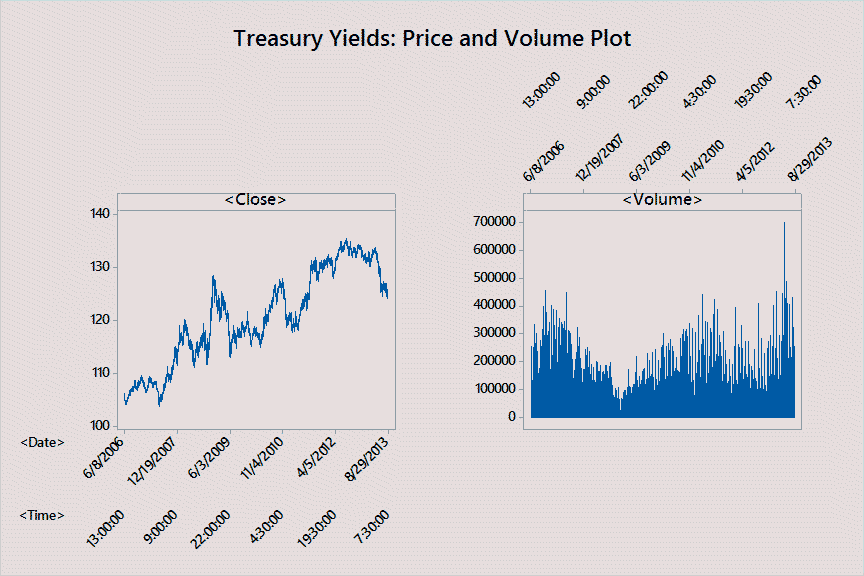
\includegraphics[width=0.8\textwidth]{chapters/chapter_stat_ts/figures/treasury.png}
   \caption{Treasury Yields: Price and Volume Plot \label{fig:treasuryyields}}
\end{figure}
\begin{figure}[!ht]
   \centering
    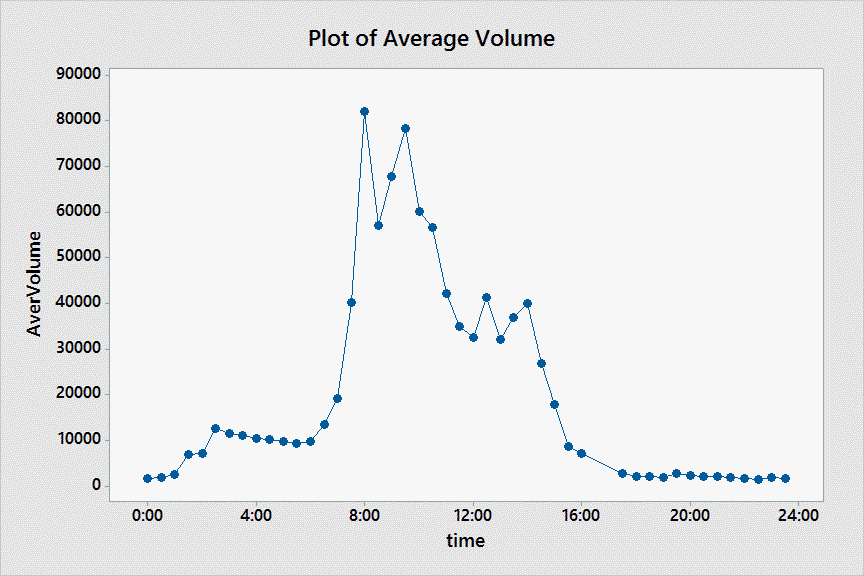
\includegraphics[width=0.8\textwidth]{chapters/chapter_stat_ts/figures/avgvol.png}
   \caption{Plot of average volume. \label{fig:averagevolume}}
\end{figure}


The plot of price and volume data is given in Figure~\ref{fig:treasuryyields}. The price data generally shows an upward trend, but it is difficult to see the pattern in volume, especially during the course of the day. A simple average volume plot clearly indicates most of the trading occurs between 8~A.M. and 4~P.M. (Figure~\ref{fig:averagevolume}). The autocorrelation function of the log volume ($v_{tm}$) clearly demonstrates the intra-day variations in the data. There is a great deal of interest among practitioners to model the volume accurately as a commonly used trading strategy, VWAP assumes that volume is known apriori. Two other benefits cited in Satish, Saxena and Palmer (2014)~\cite{satish} are if a trader receives a large order ten minutes before the close with an instruction to complete the order, having a reliable estimate of expected volume can help evaluate the feasibility of execution. The other benefit that is mentioned is how improved volume forecast can aid alpha capture. Brownlees, Cipollini and Gallo (2011)~\cite{brownless} propose a dynamic model,
	\begin{equation}\label{eqn:dynamic}
	V_{tm}= \eta_t \cdot \phi_m \cdot \mu_{t.m} \cdot \epsilon_{t.m}
	\end{equation}
where $\eta_t$ is a daily component, $\phi_m$ is the periodic component and $\mu_{t.m}$, an intra-daily dynamic, non-periodic component. The periodic component $\phi_m$ modeled as a Fourier (sine/cosine) function; the daily component is modeled as a function of past values of a daily volumes and the same is true with $\mu_{t.m}$; they are modeled as a function of $\mu_{t.m-1}$ and $V_{t.m-1}$. From the structure of the model (\ref{eqn:dynamic}), it is obvious that the multiplication components can be modeled additively through log transformations.


We suggest somewhat similar to (\ref{eqn:dynamic}) but more directly related to models discussed in Chapter 2. Before we state the results recall the main findings from past empirical studies:
	\begin{itemize}
	\item Volatility, measured by returns squared is positively correlated with volume.
	\item Large price movements are followed by high volume.
	\item Conditioning on lagged volume attenuates the leverage effect.
	\item After conditioning on lagged volume, there is positive risk-return relationship
	\end{itemize}
Our approach to modeling is stated as follows:
	\begin{itemize}
	\item Model the volume at different frequency levels.
	\item Use the low frequency data for developing macro strategies.
	\item Use the high frequency data for making micro decisions.
	\end{itemize}

\begin{figure}[!ht]
   \centering
    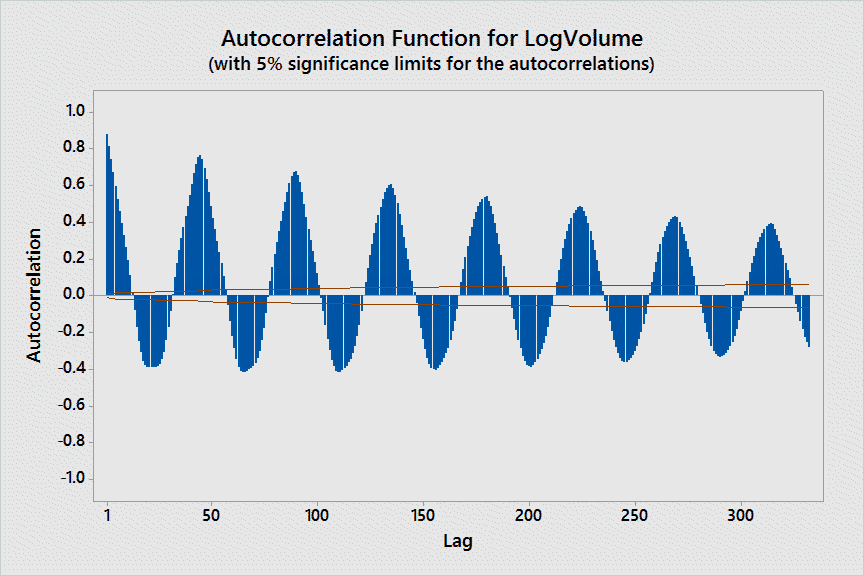
\includegraphics[width=0.8\textwidth]{chapters/chapter_stat_ts/figures/logvol.png}
   \caption{Autocorrelation function for log volume. \label{fig:logvolumeauto}}
\end{figure}
\begin{figure}[!ht]
   \centering
    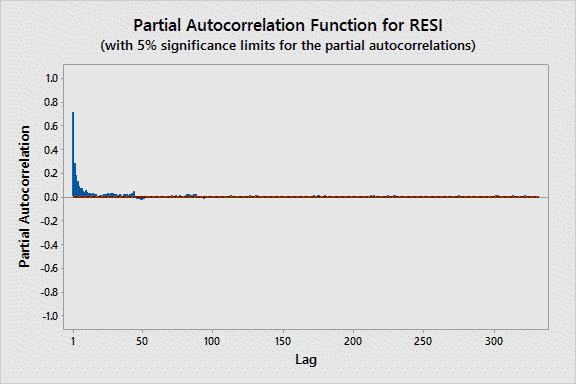
\includegraphics[width=0.8\textwidth]{chapters/chapter_stat_ts/figures/resi.png}
   \caption{Partial autocorrelation function for RESI (with 5\% significance limits for the partial autocorrelations) \label{fig:partresi}}
\end{figure}
\begin{figure}[!ht]
   \centering
    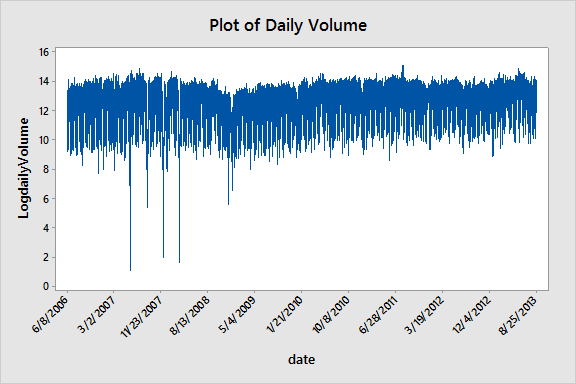
\includegraphics[width=0.8\textwidth]{chapters/chapter_stat_ts/figures/dailyvol.png}
   \caption{Plot of daily volume. \label{fig:dailyvol}}
\end{figure}


Given the strong intra-day periodicity that is evident from Figure~\ref{fig:averagevolume}, we can simply create indicator variables for the 30-min periods and regress the volume on the indicators to capture the time of the day variation. This explains almost sixty-five percent of the variation in log volume. The residuals capture non-seasonal patterns and the partial autocorrelation function is given in Figure~\ref{fig:partresi}. This clearly indicates that the residuals can be modeled as higher order autoregressive process. As these components are additive, the forecasts from indicator regression and this autoregression can be summed up to arrive at a reasonable volume forecast. The plot of logged daily volume is given in Figure~\ref{fig:dailyvol} and it is clearly stationary. The partial autocorrelation function in Figure~\ref{fig:logdailyvolume} has somewhat a simpler structure for the daily aggregated data. How do we use these results?
	\begin{itemize}
	\item Forecast next day volume using the macro model.
	\item Forecast the 30-min volume using the micro model.
	\item If the actual volume is not in line with the forecast, search if any new information has arrived!
	\end{itemize}
	
	
These methods obviously require the use of time series programs and as an alternative, we suggest using exponential smoothing approach. The details are as follows:
	\begin{itemize}
	\item Volume Forecast 1 (Direct): Use daily data to forecast $\hat{v}_{t+1}$, next day's volume; use exponential smoothing constant in the range of 0.25--0.35.
	\item Volume Forecast 2 (Aggregated): We will use a two-step procedure here:
		\begin{enumerate}[(a)]
		\item Compute the average volume $\overline{v}$ over certain number of days for each `$m$'. Usually industry uses `22' days.
		\item Compute the residuals: $e_{t\cdot m} = v_{t . m} - \overline{v}$; use exponential smoothing on $e_{t\cdot m}$ with a smoothing constant in the range of 0.25--0.35; estimate $\hat{e}_{t+1 . m}$;
		\item Forecast for next period `$m$': $\hat{v}_{t+1. m}=\overline{v}+\hat{e}_{t+1 . m}$
		\item Aggregate $\hat{v}_{t+1\cdot m}$ over $m$ to get $\hat{v}_{t+1}$. 
		\end{enumerate}
	Now we have two forecasts of daily volume $\hat{v}_{t+1}$ and $\hat{v}_{t+1}$.
	\end{itemize}
We want to relate the volume to volatility using the measure in (\ref{eqn:hatsigmasq}). Figure~\ref{fig:30min}, based on the plot of (\ref{eqn:rtsum2}) indicates that there are clustering effects. From the partial autocorrelation function given in Figure~\ref{fig:funvol}, there is some memory in the variance and can be modeled via GARCH. Here our goal is to show how volume and volatility are likely to be related. The simple cross-correlation function (Figure~\ref{fig:ccresi}) shows how they are closely related; here the intra-day periodicity in the residuals in volume and volatility is shown. Again in the spirit of intuitive approach to model the volatility, we suggest obtaining volatility forecasts as:
	\[
	\begin{cases}
	\hat{\sigma}_{t+1}^2 = \text{ weighted average of } \sigma_t^2, \sigma_{t-1}^2, \ldots, \sigma_{t-22}^2 & \\
	\hat{\sigma}^2_{t+1 \cdot m}= \text{ weighted average of } \sigma_{t\cdot m}^2, \sigma_{t-1 \cdot m}^2, \ldots, \sigma_{t-22\cdot m}^2 & 
	\end{cases}
	\]
The following algorithm that combines the price, volume and volatility is suggested; we assume the price, volume and volatility is suggested; we assume that price-based rates given in Section 3.2 are followed.
	\begin{itemize}
	\item Enter if (a) price-based rules favours and if (b) $\sigma_{t+1\cdot m}^2< \hat{\sigma}_{t+1\cdot m}^2$, realized volatility $<$ predicted volatility and if (c) $\sum_{i=1}^m v_{t+1} < \sum_{i=1}^m \hat{v}_{t+1}$, cumulative actual volume $<$ cumulative predicted volume. 
	\item Exit if either (a) or (b) or (c) is not true. 
	\end{itemize}
 
\begin{figure}[!ht]
   \centering
    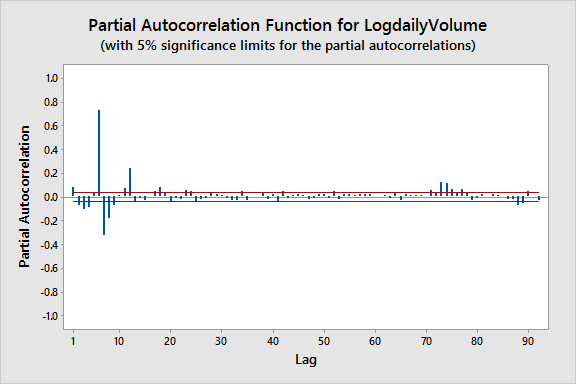
\includegraphics[width=0.8\textwidth]{chapters/chapter_stat_ts/figures/logdaily.png}
   \caption{Partial autocorrelation function for log daily volume (with 5\% significance limits for the partial autocorrelation). \label{fig:logdailyvolume}}
\end{figure}

\begin{figure}[!ht]
   \centering
    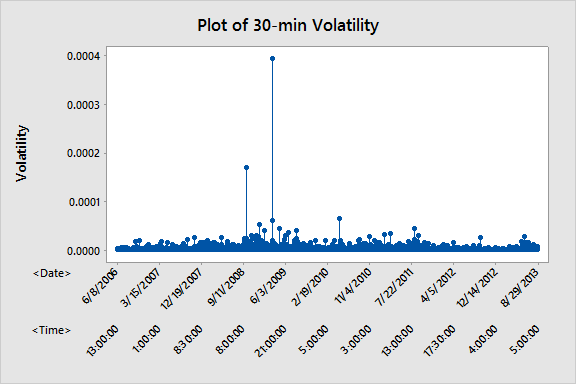
\includegraphics[width=0.8\textwidth]{chapters/chapter_stat_ts/figures/30min.png}
   \caption{Plot of 30-min volatility. \label{fig:30min}}
\end{figure}


\begin{figure}[!ht]
   \centering
    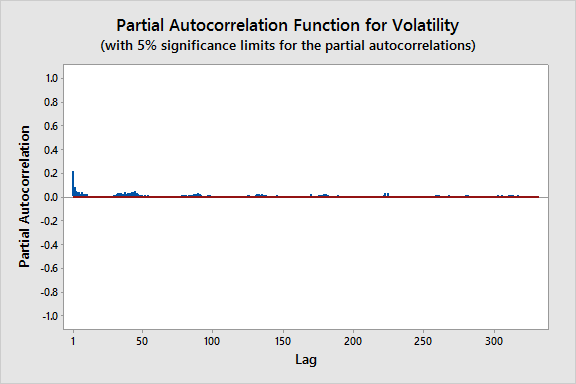
\includegraphics[width=0.8\textwidth]{chapters/chapter_stat_ts/figures/funvol.png}
   \caption{Partial autocorrelation function for volatility (with 5\% significance limits for the partial autocorrelations). \label{fig:funvol}}
\end{figure}

\begin{figure}[!ht]
   \centering
    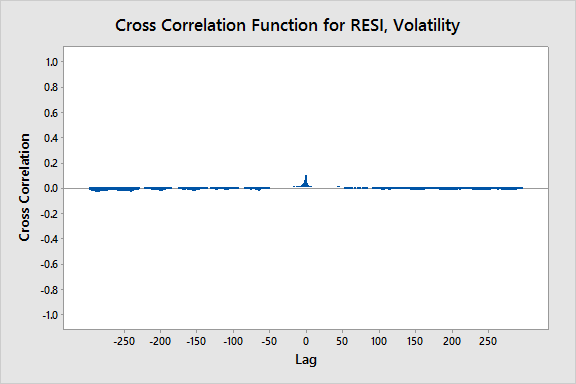
\includegraphics[width=0.8\textwidth]{chapters/chapter_stat_ts/figures/resivol.png}
   \caption{Cross correlation function for RESI, volatility. \label{fig:ccresi}}
\end{figure}






\newpage



\section{Market Segmentation and Inconsistent Pricing across Markets}

\section{Other Topics: Bet Size etc.}

\section{Supplements and Problems}


\begin{enumerate}[1.]
\item One of the most intriguing asset pricing anomalies in finance is so-called
\textquotedblleft price momentum effect\textquotedblright that was covered in this chapter. This exercise using CRSP data is meant to guide you through
creating a momentum strategy. The goal is to replicate the price momentum
strategy described in Jegadeesh and Titman (2001) \cite{JeTi} using more recent data
extending to December 2014. [This problem is based on the notes from Ravi Jagannathan.]
\hfill
\par\vspace{\baselineskip}
\textbf{A. Source of Data}
\hfill
\par\vspace{\baselineskip}
The monthly stock returns from January 1965 to December 2014 can be obtained from the web. You should construct the decile ranking by yourself. For future reference, the decile ranking file is available from Ken French's web site. The NYSE market capitalization decile contains all common shares regardless of the end of the month price.%
\footnote{%
The Fama-French factors can be downloaded from
Ken French's website. Note that you should only use the data from
\textquotedblleft U.S. Research Returns Data\textquotedblright\ section.}


You should use each stock's permanent identification code (PERMNO) as
a unique identifier for that stock.

Note that not all stocks have valid monthly returns for various reasons. One
reason is that the stock gets delisted somewhere during the month. For the
construction of your momentum portfolios, you can simply ignore the
delisting returns in your portfolio construction and return accumulations
for the sake of simplicity. More specifically, for this exercise, if the
end of the month return of any stock is missing, you may simply assume the
return is zero in your compounding. You should keep track of such
cases (identify the reason for delisting/missing observation) and prepare a
table summarizing how many such cases occured.
\hfill
\par\vspace{\baselineskip}
\textbf{B. Stocks Selection Criterion}
\hfill
\par\vspace{\baselineskip}
Consider all the common stocks traded on AMEX, NYSE and NASDAQ but
subject to the following filtering rules:

\begin{itemize}
\item Exclude all stocks priced lower than $\$5$ at the end of month ($t$).

\item Exclude all stocks belonging to the smallest NYSE market decile at the
end of month ($t$). You should first find the cutoff for the NYSE smallest
market decile, then delete all the stocks (including stocks on AMEX, NYSE,
and NASDAQ) with a market cap that's below the cutoff.
\item Another thing to take in consideration is that when you form your
portfolios, you should only apply the filters to the stocks when you form the
portfolio (i.e. at the end of month $t$). The future returns (stock returns
at month $t+2$ to $t+7$) should not be filtered. Otherwise it creates a
look-ahead bias. For example, for portfolio returns at month $t+2$ to $t+7$,
you drop stocks with a price $<$5 at any month between $t+2$ to $%
t+7$. First, when forming the portfolio at time t, you use information you
don't have at month t. Second, you eliminate stocks with likely poor
performance (low price) in the future. The portfolio returns (especially the
loser portfolio returns) are likely to be biased upward from this action.
\end{itemize}


Again, you should keep track of such cases and prepare a table
summarizing how many such cases occured..
\hfill
\par\vspace{\baselineskip}
\textbf{C. Portfolio Formation}
\hfill
\par\vspace{\baselineskip}
At the end of each month ($t$), sort the stocks into $10$ decile portfolios
based on the six month cumulative returns between month ($t-5$) to ($t$).
The first decile contains the stocks with the lowest past six-month returns,
and the tenth decile contains the stocks with the highest past six-month
returns.

\begin{itemize}
\item Start by accumulating the return of each decile portfolio between ($%
t+2 $) to ($t+7$), i.e. skipping the first month following the portfolio
formation.

\item At the beginning of each month, construct overlapping decile
portfolios as equally weighted averages of the past six month months' decile
portfolios. That is, at each month $\tau $, the $i$th overlapping decile
portfolio consists of an equal weighted average of the\ $i$th decile
portfolios of the previous six month ($\tau -5$) to ($\tau $).\footnote{%
These 10 overlapping decile portfolios are the testing assets in our asset
pricing test exercises.}

\item For each month and of the 10 overlapping decile portfolios, record the
portfolio returns between January 1995 and December 2014.
\end{itemize}
\hfill
\par\vspace{\baselineskip}
\textbf{D. Questions of Interests}
\hfill
\par\vspace{\baselineskip}
After constructing the relevant portfolios, answer the following questions.
When you answer these questions, note any additional assumptions/choices you
made.
\hfill
\par\vspace{\baselineskip}
\textbf{E. Momentum strategy profits.}
\hfill
\par\vspace{\baselineskip}
\begin{enumerate}
\item Report the monthly average returns of your overlapping decile
portfolio, as well as the winner ($P1$, highest past six month return
portfolios) minus losers ($P10$, lowest past six month return portfolios).

\item Report the monthly average returns of your overlapping decile
portfolio for January and non-January months respectively, as well as the
winner ($P1$, highest past six month return portfolios) minus losers ($P10$,
lowest past six month return portfolios).

\item Using CAPM and Fama-French version of multifactor asset pricing model
to test the spreads between winner and loser portfolio ($P10$ - $P1$). \ The
Fama-French factors can be obtained from Kent French's web site.

\item Tabulate these results in a table similar to table $I$ in Jegadeesh
and Titman (2001).

\item Compared your results to the results in Jegadeesh and Titman (2001)
\emph{and comment on your findings.}
\end{enumerate}
\hfill
\par\vspace{\baselineskip}
\textbf{F. Momentum strategy and market capitalization.}
\hfill
\par\vspace{\baselineskip}
\begin{enumerate}
\item Repeat the above exercise but split the sample into small-cap and
big-cap portfolio, where the small-cap portfolio contains the stocks in the
lower five NYSE\ market capitalization deciles.

\item Tabulate these results in a table similar to table $I$ in Jegadeesh
and Titman (2001).

\item Compare the simple momentum strategy's profits, and momentum strategy
cut by the market capitalization profits to value-growth strategy's return.
The value-growth strategy return can be proxied by the HML factor obtained
from Ken French's website.

\item \emph{Comment on your findings}. In particular, briefly suggest at
least three reasons why momentum profits may be related to market
capitalization, and how would you go ahead and test it further.
\end{enumerate}
\hfill
\par\vspace{\baselineskip}


\item One of the commonly used trading strategies in finance the so-called ``pairs trading'' is covered in this chapter. This is an exercise to replicate the strategy. Obtain the daily data from January 2000 to June 2014 on stock prices, returns, trading volume and shares outstanding on the following companies only: \\

\noindent Oil stocks: HAL, SLB, EQT, OXY, CVX \\

\noindent Tech stocks: AAPL, CSCO, GOOG, INTL, MSFT \\

\noindent Bank stocks: BAC, JPM, WFC, C, STI \\

\noindent Retail stocks: ANF, GES, SKS, SHLD, URBN \\


Begin forming pairs in January 2000 based on the estimation period, January 2000 to December 2000. The last estimation period is January 2014 to December 2014. Eligible pairs corresponding to the last estimation remain eligible till December 2014. Pairs that opened in December 2013 and did not converge with the stipulated maximum of six months would have been closed in June 2014.


As you recall, the pairs trading strategy works as follows:
\begin{enumerate}[(a)]
\item Within each sector, match pairs based on normalized price differences over the past year.

\item When a tracked pair diverges by more than two standard deviations of their normalized price difference, buy the ``cheap'' stock and sell the ``expensive'' one after a one-day wait period (to mitigate the effects of any market irregularities).

\item If prices for a traded pair re-converge, exit the paired positions.

\item If prices for a traded pair do not re-converge within six months, close the positions. An alternative strategy closes all traded pairs in ten trading days.
\end{enumerate}


Questions of interest:
\begin{enumerate}[a.]
\item Quantify the profitability of the pairs trading strategy and on average, how long it takes for pairs to re-converge?

\item Can you provide some insight into why the strategy works based on trading volume, shares outstanding and the market trend?


    Note: As minimum, you are supposed to produce figures similar to figures 1-5 of the paper as well as Table 1


    Another Question of interest
\item Is there a pair across sectors that can outperform the pairs formed within each sector?
\end{enumerate}
\hfill
\par\vspace{\baselineskip}


\item The file Exchange rates.csv contains exchange rates between US\$ and 25 major currencies; the daily data spans from Jan 3, 2000 to April 10, 2012. Consider the data from Jan 3, 2002 for the following currencies: EUR, GBP, DKK, JPY and CNY. Compute $r_t = \ln{p_t} - \ln{p_{t-1}}$, returns for each series.

\textbf{A.}
\begin{minipage}[t]{0.8\linewidth}
\begin{enumerate}[(a)]
\item Estimate the mean vector and the covariance matrix of the returns.
\item Construct a portfolio with Markowitz's minimum variance objective with expected returns at least R, the median of the elements in the mean vector. The weights must be positive and should sum to 1.
\item Repeat (a) and (b) for each year and comment on the variation in the composition of the portfolios.
\end{enumerate}
\end{minipage}

\textbf{B. Evaluation of Trading Rule:} Consider the data starting June 11, 2003.
\begin{enumerate}[(a)]
\item Compute the average return for each day. We will treat this a `market' return.
\item Consider the two currencies: EURO and JPY and assume that your investment is restricted to only these two currencies. We will follow the simple algorithm: if 
\hfill
\par\vspace{\baselineskip}
    $$ \frac{r_i - \overline{r}}{sd(r_i)}=\left\{
\begin{aligned}
> 2 \hspace{1cm}sell \\
< -2 \hspace{1cm}buy \\
o.w. \hspace{1cm}hold
\end{aligned}
\right.
$$
The average and standard deviation of the returns are based on last 30-day observations. Evaluate this algorithm by comparing it with simple holding.
\item What is the value of the `market' return? How could this information be used?
\end{enumerate}

\textbf{C. Trading Rule with other factors:} In addition to exchange rates from June 11, 2003, consider the data on commodity prices: Gold, Oil, Copper and a commodity index. Among the following currencies, CAD, BRL, ZAR, AUD, NZD, CAF and RUB, which are most influenced by the commodity prices. Discuss how you would incorporate this into a trading strategy.
\item  This homework consists of an exercise on `pairs trading' using CRSP data which will guide you through creating that strategy. The goal is to replicate the strategy as described in Engelberg, Gao and Jagannathan (2009)~\cite{engelberg2009anatomy}. Focus only on sections 1,2 and 4 of the paper. Obtain the daily data from January 1992 to June 2010 on stock prices, returns, trading volume and shares outstanding on the following companies only:
    \hfill
\par\vspace{\baselineskip}
    DELL, HP, ADBE, MSFT, AAPL\hfill \break
JPM, WFC, BAC, C, BRK.A\hfill \break
JNJ, WMT, COST, KO, PEP\hfill \break
GM, TM, F\hfill \break
XOM, COP
\hfill
\par\vspace{\baselineskip}


``Begin forming pairs in January 1993 based on the estimation period, January 1992 to
December 1992. The last estimation period is January 2009 to December 2009. Eligible pairs
correponding to the last estimation remain eligible till December 2009. Pairs that opened
in December 2009 and did not converge with the stipulated maximum of six months would
have been closed in June 2010.''


As you recall, the pairs trading strategy works as follows:
\begin{enumerate}
\item Match pairs based on normalized price differences over the past year.
\item When a tracked pair diverges by more than two standard deviations of their normalized price difference, buy the ``cheap'' stock and sell the ``expensive'' one after a one-day wait period (to mitigate the effects of any market irregularities)
\item If prices for a traded pair re-converge, exit the paired positions.
\item If prices for a traded pair do not reconverge within six months, close the positions. An alternative strategy closes all traded pairs in ten trading days.
\end{enumerate}
Question of interest:
\hfill
\par\vspace{\baselineskip}
\begin{enumerate}
\item[1.] Quantify the profitability of the pairs trading strategy and on average, how long it takes for two pairs to reconverge?
\item[2.] Can you provide some insights into why the strategy works based on trading volume,
shares outstanding and the market trend?
\end{enumerate}
Note: as a minimum, you are supposed to produce figures similar to figure 1-5 of the
paper as well as table 1.
\item{\it Technical Rules}

Consider the data on exchange rates between the Indian Rupee and the US Dollar, British Pound and Euro. In order to compare the performance of a strategy, appropriately normalize the entry point exchange rate: invest equal amounts of capital (counted in INR, which we will call the ``base currency'') in each trade. Total portfolio return on each day should be computed as a weighted sum of returns from each active trade (weighted by the current value of each trade). Evaluate the signals discussed in (a) and (b) below using the Sharpe ratios and PNL with and without including transaction costs of $15$ basis points. Assume a risk free rate of $3\%$. (1 basis point = $10^{-4}$; so each dollar traded costs $0.0015$ in transaction costs)
\begin{enumerate}
\item{\it Moving average trading rules}: Trading signals are generated from the relative levels of the price series and a moving average of past prices.
\begin{itemize}
\item  Rule 1: Let $\overline{p}_t^{(m)}$ as defined in (4); use the strategy to sell if $p_t>\overline{p}_t^{(m)}$ and to buy if  $p_t<\overline{p}_t^{(m)}$. Evaluate this strategy. What is the optimal ``$m$''?
\item Rule 2 (Bollinger rule): Use the Bollinger rule as outlined in the text; what is the optimal ``$m$''?
\item Rule 3 (Resistance-Support): Buy if $p_t > \max_{\substack{0\le i< m}}p_{t-i}$ and sell if $p_t < \min_{\substack{0\le i< m}}p_{t-i}$. Evaluate this rule. What is the optimal ``$m$''?
\item Rule 4 (Momentum): Compute a short-term moving average over the last $m$ prices, $\overline{p}_t^{(m)}$ and a long-term average over the last $n$ prices, $\overline{p}_t^{(n)}$ with $m<n$. If $\overline{p}_t^{(m)}$ crosses $\overline{p}_t^{(n)}$ from below, sell and if it crosses $\overline{p}_t^{(n)}$ from above, buy. Evaluate this strategy. What are the optimal values of $m$ and $n$ ?
\end{itemize}
\item{\it RSI Oscillator Rule}: Use $\text{RSI}_t$ as defined in (5). \hfill \break
If $\text{RSI}_t<30$, buy and if $\text{RSI}_t>70$, sell. Evaluate this trading strategy. What is the optimal ``$m$''?

\item {\it Pairs Trading: Distance Method}

We want to develop a pairs trading strategy and check if it does any better than  the strategies in Problem 1. At the last trading day of the month, look back 3 months and identify if any pairs are worth trading. Use the distance measures, thresholds, and portfolio return accounting as given in Engleberg, et al. (2009, p2-4). Summarize the results using the same format as in Problem 1.

\item {\it Pairs Trading: Cointegration Method}

In the cointegration method, we can consider the possibility of trading more than 2 assets. Check using a moving window of 3 months which series are cointegrated. Develop appropriate trading strategies to trade portfolios formed from the cointegrating vectors and compare with the pairs trading strategies from Problem 2. (You may use and extend the ideas from Problem 2 to concretely define the trading indicators and thresholds for entry and exit.) Summarize the performance results as in Problem 1.

\item {\it Pairs Trading: APT method}

Consider the data with the S\&P500 market index returns and assume that the risk free rate is 3\%. Regress each currency's excess return (over the risk free rate) on the excess market return over a moving window of 3 months. Find pairs based on the similarity of the regression coefficients.
\begin{enumerate}
\item Compare the pairs that result from the APT method with those obtained in Problem 2.
\item After finding the pairs, use the same rules as in Problem 2 to decide when to enter and exit specific trades.
\end{enumerate}
Summarize the performance results as in Problem 1.

\item {\it Summing up}

Provide a summary table with the main findings and drawbacks of all the methods that are explored in this assignment. In particular, comment on the performance of single-asset strategies versus multi-asset strategies. Also comment on whether the market factor adds any value.
\end{enumerate}
\item This exercise using data for sixteen stocks will guide you through creating a momentum strategy. The goal is to replicate the price momentum strategy described in Jegadeesh and Titman (2001) using this data, albeit in a small scale. [Solution available on Web.]
    \begin{enumerate}[6.1]
    \item \textbf{Data} \hfill \break
    The daily returns from January 11, 2000 to November 20, 2005 for sixteen stocks are in the file d\_logret\_16stocks;
to this add two more columns: SP500 returns and risk free rate.
    \item \textbf{Portfolio Formation} \hfill \break
    On the last day of each month, sort the stocks into four quartile portfolios based on the past six month
cumulative returns. The first quartile contains the stocks with the lowest past six-month returns, and the
fourth quartile contains the stocks with the highest past six-month returns.
        \begin{enumerate}[(a)]
        \item Start by accumulating the return of each quartile portfolio for next six months
        \item For each month and of the four quartile portfolios, record the average portfolio returns between January 2002 and November 2005.
        \end{enumerate}
    \item \textbf{Questions of Interests} \hfill \break
    After constructing the relevant portfolios, answer the following questions. When you answer these questions, note any additional assumptions/choices you made.
    \hfill
\par\vspace{\baselineskip}
    6.3.1 Momentum strategy profits
    \begin{enumerate}[1.]
    \item Report the monthly average returns of your quartile portfolio, as well as the winner (Q4, highest
past six month return portfolios) minus losers (Q1, lowest past six month return portfolios).
    \item Report the monthly average returns of quartile portfolio for January and non-January months respectively, a well as the winner (Q4, highest past six month return portfolios) minus losers (Q1, lowest
past six month return portfolios).
    \item Using CAPM test the spreads between winner and loser portfolio (Q4-Q1).
    \item Tabulate these results in a table similar to table I in Jegadeesh and Titman (2001).
    \item Compare your results to the results in Jegadeesh and Titman (2001) and comment on your findings.
    \end{enumerate}
    \end{enumerate}
    
    
\item Consider the 30-min price bar data for Treasury Yields from June 8, 2006 to August 29, 2013. Daily data for Treasury Yields is just a snapshot at 4 pm and the total volume for the day is the sum of 30-min volumes since the previous day. [Solution available on Web.]
   \begin{enumerate}
   \item Develop ARMA time series models for both daily and the 30-min volumes. We can use daily data
for developing macro strategies and 30-min data for micro strategies.
\item Compare the exponential smoothing approach suggested in the text with ARMA modeled in (a).
   \item Compute volatility measure, $\sigma_t^2 = 0.5[\ln{\frac{H_t}{L_t}}]^2 - 0.386[\ln{\frac{C_t}{O_t}}]^2$ for both levels and compare them
   \item Compute volatility forecasts, $\hat{\sigma}_{t+1}^2$ = weighted average of $\sigma_{t}^2, \sigma_{t-1}^2,...,\sigma_{t-22}^2$, for daily data and $\hat{\sigma}_{t+1\cdot m}^2$ = weighted average of $\sigma_{t\cdot m}^2,...,\sigma_{t-22\cdot m}^2$ for $m^{th}$ 30-min interval. [ In (a), you should notice strong seasonality in the 30-min data]
   \item Develop trading strategies that incorporate
      \begin{enumerate}
      \item price information only
      \item price and volume information and
      \item price, volume and volatility information
      \end{enumerate}
         \item Demonstrate that volume and volatility add value to the enter/exist strategies.
   \end{enumerate}
   \hfill
\par\vspace{\baselineskip}

\end{enumerate}

% !TEX root = ../../book.tex
%\hfill
%\par\vspace{\baselineskip}

\chapter{Active Portfolio Management and Dynamic Investment Strategies}

\section{Introduction to Modern Portfolio Theory}


Of fundamental interest to financial economists is to examine the relationship between the risk of a financial security and its return. While it is obvious that risky assets can generally yield higher returns than risk-free assets, a quantification of the tradeoff between risk and expected return was made through the development of the Capital Asset Pricing Model (CAPM) for which the groundwork was laid by Markowitz (1959)~\cite{markport}. A central feature of the CAPM is that the expected return is a linear function of the risk. The risk of an asset typically is measured by the covariability between its return and that of an appropriately defined `market' portfolio. Examples of expected return-risk model relationships include the Sharpe (1964)~\cite{sharpcap} and Lintner (1965)~\cite{lint65} CAPM, the zero-beta CAPM of Black (1972)~\cite{blackcap}, the arbitrage pricing theory (APT) due to Ross (1976)~\cite{rossarb} and the intertemporal asset pricing model by Merton (1973)~\cite{mertonint}. The economy-wide models developed by Sharpe, Lintner and Black are based on the work of Markowitz which assumes that investors would hold a mean-variance efficient portfolio. The main difference between the works of Sharpe and Lintner and the work of Black is that the former assume the existence of a risk-free lending and borrowing rate whereas the latter derived a more general version of the CAPM in the absence of a risk-free rate.


In this section, we briefly review the CAPM model and the implications for empirical research in the area of portfolio construction and testing. 



\subsection{Mean-Variance Portfolio Theory}


A portfolio which is composed of individual assets has its risk and return characteristics based on its composition and how the individual asset characteristics correlate with each other. The optimal combination is designed to produce the best balance between risk and return. For a given level of return, it will provide the lowest risk and for an acceptable level of risk, it will provide the maximum return. The locus of the combination of risk and reward that characterizes the optimal portfolios is called the ``Efficient Frontier.''


We follow the same conventions as before to denote the return as $r_t=\ln(P_t) - \ln(P_{t-1})$; assume we have `$m$' assets in the portfolio with `$w_i$' denoting the share value invested in asset, `$i$', if $R_t=(P_t-P_{t-1})/P_{t-1}$, the portfolio return is $R_{pt}=\sum_{i=1}^m w_i R_{it}$ and thus $r_t=\ln \left(1+\sum_{i=1}^m w_i R_{it} \right) \simeq \sum_{i=1}^m w_i r_{it}$. If $r_t$ denotes the vector of `$m$' asset returns and with weights stacked up as a vector, $w$, then $r_{pt}=w' r_t$ resulting in $\mu_p=E(r_{pt})=w' \mu$ and $\sigma_p^2=w' \Sigma w$, where $\Sigma$ is the $m\times m$ variance-covariance matrix of $r_t$. If the returns are uncorrelated or negatively correlated, then observe that
	\begin{equation}\label{eqn:5sigmap}
	\sigma_p^2= w' \Sigma w \leq \sum_{i=1}^m w_i \Var(r_{it}) \leq \dfrac{v}{m}
	\end{equation}
where `$v$' is the maximum of $\Var(r_{it})$, clearly indicating that diversification tends to reduce risk. The power of the diversification can be seen clearly if we assume the covariance matrix, $\Sigma$, has all variances equal and if all off-diagonal covariance elements are the same. Then, $\sigma_p^2=\frac{1}{n} \cdot \sigma^2 + \frac{n-1}{n} \cdot \rho \cdot \sigma^2$. Observe that if $\rho=0$, $\sigma_p^2 \to 0$ as $n \to \infty$ and if $\rho=1$, $\sigma_p^2=\sigma^2$ that results in no benefit. When $\rho<0$ as shown in (\ref{eqn:5sigmap}), the portfolio variance is less due to diversification. But it should be noted that we cannot completely eliminate portfolio risk when the correlations among the assets are positive. Observe that $\sigma_p^2= \frac{1}{m^2} \sum_{i=1}^m \sigma_i^2 + \frac{1}{m^2} \sum_{i \neq j} \sigma_{ij} \leq \frac{\sigma_{\text{max}}^2}{m} + \frac{m-1}{m} \cdot A \to A$ as $m \to \infty$. \\


\noindent \textbf{Minimum Variance Portfolio:} The efficient portfolio is obtained through the constrained optimization:
	\begin{equation}\label{eqn:5opt}
	\min_w w' \Sigma w \enskip \ni w' \mu = \mu^*, \quad w'1=1
	\end{equation}
Here 1 is the $m \times 1$ unit vector. The solution to this can be obtained via Lagrangian function and can be found in Campbell, Lo and MacKinley (1996, Section 5.2)~\cite{campbellmaclo}. With $A=1' \Sigma^{-1} \mu$ (weighted mean), $B=\mu' \Sigma^{-1} \mu$ ($F$-ratios), $C=1'\Sigma^{-1}1$ and $D=BC-A^2$, the `weight' vector, $w$, is given as,
	\begin{flalign}\label{eqn:5effdoub}
	&& w_{\text{eff}}&= \{ B \Sigma^{-1} 1- A \Sigma^{-1}\mu + \mu^*(C\Sigma^{-1} \mu- A\Sigma^{-1}1)\}/D && \notag \\
	\text{and} && \phantom{x} & \phantom{x} && \\
	&& \sigma_{\text{eff}}^2&= (B-2\mu^*A+\mu^{*2}C)/D && \notag
	\end{flalign}
The graph of the efficient frontier $(\mu^*, \sigma_{\text{eff}})$ in the mean-standard deviation space is the right side of a hyperbola (see Figure~\ref{fig:frontier}).

	\begin{figure}[h!]
	   \centering
	   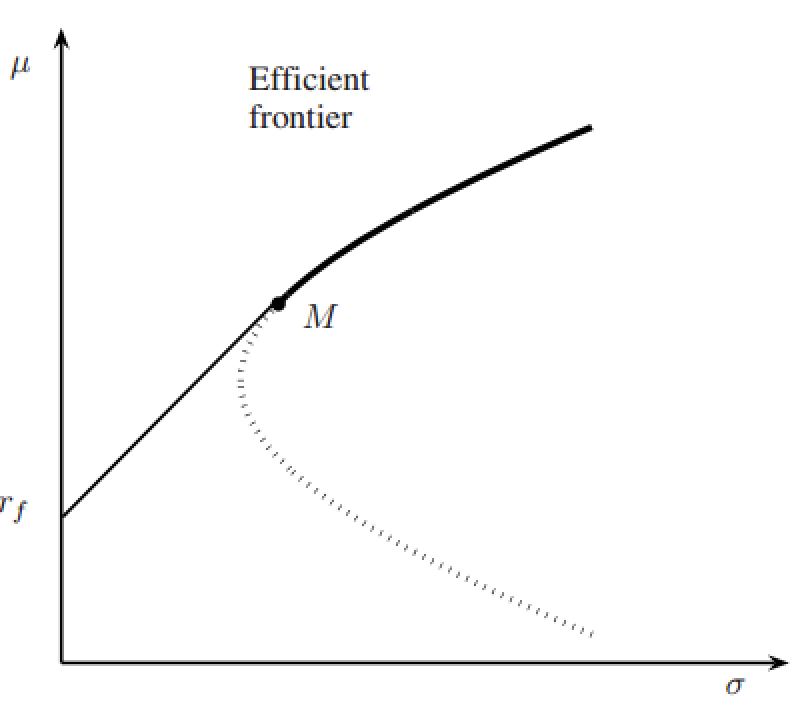
\includegraphics[width=0.6\textwidth]{chapters/chapter_apm/figures/frontier.png} 
	   \caption{Efficient frontier with no short selling. \label{fig:frontier}}
	\end{figure}
It must be noted that in the formulation (\ref{eqn:5opt}), the weights can be negative implying that short selling is allowed. With no short selling, $w_i \geq 0$ for all `$i$', there is no explicit solution but can be numerically solved via quadratic programming. 


Suppose an investor is interested in a portfolio with maximum Sharpe ratio $=$ average return/standard deviation, which represents the return per unit risk. Graphically, the portfolio is the point where a line through the origin is tangent to the efficient frontier, because this point represents the highest possible Sharpe ratio. So it is called the tangency portfolio. The inverse of the slope is obtained by setting $\frac{\delta \sigma^2_{\text{eff}}}{\delta \mu^*}=0$ which yields $\mu^*=A/C$ and $\sigma_{\text{MV}}^2=\frac{1}{C}$ and the efficient combination is simply, $w_{\text{MV}}=\Sigma^{-1} \mu/C$. Thus we have described two portfolios that an investor can prefer. If minimum amount of risk is desired, the minimum variance portfolio is taken and if the objective is to maximize the Sharp ratio, the tangency portfolio is taken. These can be formulated from the point of view of unified theory of utility maximization. 


Assume that the utility function is given as,
	\begin{equation}\label{eqn:utility}
	u= w' \mu - \frac{\lambda}{2} \,w' \,\Sigma \,w
	\end{equation}
where `$\lambda$' is called the parameter of absolute risk-aversion. The greater the `$\lambda$', the more risk averse the investor is. Usually $2<\lambda<4$. Thus assuming all investors are risk-averse, the objective function is,
	\begin{equation}\label{eqn:5maxu}
	\max_w u \enskip \ni \enskip w'1=1
	\end{equation}
It can be easily shown that the resulting weight vector is,
	\begin{equation}\label{eqn:5weff}
	w_{\text{eff}}= \dfrac{1}{\lambda} \left(\Sigma^{-1} \mu + \Sigma^{-1} 1 \cdot \gamma^*\right)
	\end{equation}
where $\gamma^*=(\lambda-A)/C$. The results can be obtained again using Lagrangian multipliers and the matrix differentiation results $\left( \frac{\delta \Sigma w}{\delta w}= \Sigma; \frac{\delta(w'\Sigma w)}{\delta w})=2 \cdot w' \Sigma\right)$. From (\ref{eqn:5weff}) observe that it is a combination of minimum variance portfolio and the tangency portfolio. At the optimum point, note
	\begin{flalign}\label{eqn:5effdoub1}
	&& \mu_{\text{opt}}&= w' \mu= \dfrac{D}{\lambda C}+\mu_{\text{MV}} && \notag \\
	\text{and} && \phantom{x} & \phantom{x} && \\
	&& \sigma^2_{\text{opt}}&= w'\Sigma w= \sigma^2_{\text{MV}} + \dfrac{1}{\lambda^2} \cdot \dfrac{D}{C} && \notag
	\end{flalign}
If an investor is fully risk-averse, $\lambda \to \infty$ and the optimal portfolio is the minimum variance portfolio and when $\lambda=A$, the optimum portfolio is the tangency portfolio. Thus both are special cases of Markowitz strategy. 


For realistic situations related to trading we need to consider borrowing and lending at the risk-free rate, `$r_f$'. We assume that in addition to `$m$' risky assets, where investment is made, there is a possibility of putting the funds in the risk-free assets such as treasury bonds or CD's etc. The optimization problem can be stated as,
	\begin{equation}\label{eqn:5min2}
	\min_w w' \Sigma w \ni w'\mu + (1-w'1) r_f = \mu^*
	\end{equation}
This results in efficient weights:
	\begin{equation}\label{eqn:5weff2}
	w_{\text{eff}}= \dfrac{\mu^* - r_f}{(\mu - r_f1)' \Sigma^{-1}(\mu - r_f 1)} \cdot \Sigma^{-1}(\mu - r_f1)
	\end{equation}
If $w_i$'s are set $\geq 0$, there is no explicit analytic solution and the Figure~\ref{fig:frontier} depicts the optimal allocation. When $w_i$'s are unrestricted, the efficient frontier based on all risky assets is given as, 
	\begin{equation}\label{eqn:5murf}
	\mu= r_f + \dfrac{\mu_m - r_f}{\sigma_m} \cdot \sigma
	\end{equation}
which is known as capital market line or the security market line; here $\mu_m$ can be the return from S\&P500 index. The form of (\ref{eqn:5murf}) lends itself for empirical testing via the regression model,
	\begin{equation}\label{eqn:5ritrf}
	r_{it} - r_f = \beta_i (r_{mt} - r_f) + \epsilon_{it}
	\end{equation}
where $\beta_i=\Cov(r_{it},r_{mt})/\sigma_m^2$; note the volatility in `$r_i$' can be decomposed as 
	\begin{equation}\label{eqn:5sigsq}
	\sigma_i^2= \beta_i^2 \sigma_m^2 + \sigma_\epsilon^2.
	\end{equation}
If $\beta_i>1$, the asset is taken to be aggressive. The commonly used performance indices follow from the population version of the model (\ref{eqn:5ritrf}) which is $\mu - r_f = \alpha + \beta(\mu_m - r_f)$. Sharpe index is given as $(\mu- r_f)/\sigma$, Treynor's index is $(\mu- r_f)/\beta$ and Jensen's index is simply the `$\alpha$'. If $\alpha>0$, it is taken that the portfolio performs better than the market after adjusting for the risk. 


The CAPM model is empirically tested via (\ref{eqn:5ritrf}) with added intercept terms:
	\begin{equation}\label{eqn:intercept}
	r_{it} - r_f = \alpha_i + \beta_i (r_{mt} - r_f) + \epsilon_{it}
	\end{equation}
If CAPM holds then $H_0: \alpha_i=0$, $i=1,2,\ldots,m$ should be supported. But empirical evidence does not seem to support $H_0$; various explanations are possible. It is argued that the proxies such as S\&P500 index are not theoretically true market portfolio which is supposedly based on all assets. It has been shown that other asset related information provide better explanatory power for the cross-sectional variation of the asset returns. This has led to multi-factor models that is discussed next. 


\subsection{Multifactor Models}


Ross (1976)~\cite{rossarb} introduced the Arbitrage Pricing Theory (APT) which is more general than CAPM; the cross-sectional variation in the asset returns, it is postulated may be due to multiple risk factors. There is no need to identify a market portfolio nor the risk-free return. The model can be written as:
	\begin{equation}\label{eqn:arbrit}
	r_{it} = \alpha_i + \beta_i' f_t + \epsilon_t
	\end{equation}
and given $f_t$ is a $n \times 1$ vector of factors, $E(\epsilon_{it})=0$, $E(\epsilon_{it}\epsilon_{jt})=\sigma_{ij}$, $i,j =1,2,\ldots,m$ and $t=1,2,\ldots, T$. In the absence of arbitrage, Ross (1976)~\cite{rossarb} shows that the following relationship should hold:
	\begin{equation}\label{eqn:mewirf}
	\mu_i \sim r_f + \beta_i' \lambda_k
	\end{equation}
where $\lambda_n$ is a $n \times 1$ vector of factor risk premia.


Generally, there are two approaches to empirically model (\ref{eqn:arbrit}) and test if (\ref{eqn:mewirf}) holds. In the first approach, it is assumed that the factors ($f_t$) are unknown and are estimated from the ($m \times m$) covariance matrix of the returns via principal components. The number of factors, $n$, is generally determined via subjective considerations. In the second approach, it is taken that the factors are determined by macroeconomic variables that reflect systematic risk and by asset characteristics. Chen, Roll and Ross (1986)~\cite{chenecforce} consider expected inflation, spread between high and low grade bond yields, spread between long and short interest rates for U.S. government bonds etc. as known factors. The asset characteristics that are noted to be useful are: ratio of book to market value, price-earnings ratio, momentum, Farma-French factors. These factor models with known or unknown factors tend to fare better than CAPM. As we will demonstrate, they are also useful for the construction of the portfolios as these factors are likely to represent different risk dimensions. 

	
\subsection{Tests Related to CAPM and APT}


To test if any particular portfolio is ex ante mean-variance efficient, Gibbons, Ross and Shanker (1989)~\cite{gibbons} provide a multivariate test statistic and study its small sample properties under both null and alternative hypotheses. This follows from the multivariate regression model and the associated test procedures discussed in the last section. Recall the null hypothesis is:
	\begin{equation}\label{eqn:secnull}
	H_0: \alpha_i=0 \enskip \forall i=1,2,\ldots,m
	\end{equation}
The test statistic is a multiple of Hotelling's $T^2$ stated as,
	\begin{equation}\label{eqn:hotelT}
	F= \dfrac{T-m-1)}{m} \cdot \dfrac{\hat{\alpha}' \hat{\Sigma}_{\epsilon\epsilon}^{-1} \hat{\alpha}}{1+\hat{\theta}_p^2} \sim F(m,T-m-1)
	\end{equation}	
where $\hat{\theta}_p= \overline{r}_p/s_p$, the ratio of sample average and standard deviation of $r_{pt}$. The noncentrality parameter depends on $\alpha' \Sigma_{\epsilon\epsilon}^{-1} \alpha$ which is zero under $H_0$. The statistical power of the $F$-test thus can be studied. The test statistic in (\ref{eqn:hotelT}) can be easily derived from the results on multivariate regression by setting $F_1=I_m$ and $G_2=\gamma^*=(1,0)'$. The constrained ML estimator of $C$ under (\ref{eqn:secnull}) is $\hat{C}=\tilde{C} \left[I_2 - \dfrac{\gamma^* \gamma^{*'} (x\gamma')^{-1}}{\gamma^{*'}(x\gamma')^{-1} \gamma^*}\right]$. Thus we can compute the residual covariance matrices both under the null and alternative hypotheses to arrive at the LR statistic. 


A practical question that needs to be resolved is on the choice of `$m$' and `$T$'. With over 5000 stocks listed in NYSE and with daily data available since 1926, the choice is restricted only by the condition $T>m$ for the variance-covariance matrix in the estimation of the model (\ref{eqn:intercept}) to be non-singular. Gibbons et al. (1989)~\cite{gibbons} suggest `$m$' should be roughly a third to one half of `$T$'. Then it is also important to decide which `$m$' assets are to be chosen. One suggested approach is to use beta-sorted assets but it may not necessarily give better power to the $F$-test. 
	
	
Note that $H_0: \alpha=0$, where $\alpha'=(\alpha_1,\ldots,\alpha_m)$ is violated if and only if some portfolio of the assets considered in the regression model (\ref{eqn:intercept}) have non-zero intercept. If we write $\hat{\alpha}$ as the $m\times 1$ vector of estimates of the intercepts, then for a linear combination of $a'r_t$, where $r_t$ is the $m \times 1$ vector of asset returns, [observe that if we let $Y_t=r_t-r_f1$ and $X_t=[1,r_{mt}-r_f]'=[1,x_t]'$, $a'Y_t=a' \alpha + (a'\beta) x_t + \epsilon_t$, and thus] $\Var(a'\hat{\alpha})= (1+\hat{\theta}_p^2) \frac{a' \hat{\Sigma}a}{T}$ and hence
	\begin{equation}\label{eqn:smallt}
	t_a^2= \dfrac{T(a'\hat{\alpha})^2}{(1+\hat{\theta}_p^2)(a' \hat{\Sigma} a)}
	\end{equation}
Maximizing $t_a^2$ is therefore equivalent to minimizing $a' \hat{\Sigma}a$ subject to $a'\hat{\alpha}=C$ as in (\ref{eqn:5sigmap}), this is equivalent to the portfolio minimization problem. The solution is
	\begin{equation}\label{eqn:5a}
	a= \dfrac{C}{\hat{\alpha}' \hat{\Sigma}^{-1} \hat{\alpha}} \cdot \hat{\Sigma}^{-1} \hat{\alpha}
	\end{equation}
and thus $t_a^2= T \cdot \frac{\hat{\alpha}' \hat{\Sigma}^{-1} \hat{\alpha}}{1+\hat{\theta}_p^2}= \frac{T}{T-m-1} \cdot m \cdot F$. Thus `$a$' can provide information about creating a better model. The portfolio based on `$a$' can provide information about creating a better model. The portfolio based on `$a$' is termed as an active portfolio and Gibbons et al. show that when this is combined with the `market' portfolio series in ex post efficient portfolio. To make the comparison between the three portfolios, average returns for all three are set equal which results in the choice of $C=\overline{r}_m \cdot \frac{\hat{\alpha} \hat{\Sigma}^{-1} \hat{\alpha}}{\hat{\alpha}' \hat{\Sigma}^{-1} \hat{\gamma}}$ and thus the active portfolio results in 
	\begin{equation}\label{eqn:5a2}
	a= \overline{r}_m \cdot \dfrac{\hat{\Sigma}^{-1} \hat{\alpha}}{\hat{\alpha}' \hat{\Sigma}^{-1} \overline{r}}
	\end{equation}	
which can be compared with $w_{\text{eff}}$ in (\ref{eqn:5effdoub}). It must be noted that the weights obtained in (\ref{eqn:5effdoub}) are not in reference to any other portfolio and not adjusted for any comparison with other portfolios. Thus one could expect that the two portfolios would be the same only when the assets selected are not correlated to market index or to any benchmark portfolio. 


The test for APT model for known factors in (\ref{eqn:arbrit}) also follows easily from the multivariate regression results discussed in the last section. The model can be restated as
	\begin{equation}\label{eqn:5rtalpha}
	r_t = \alpha + B f_t + \epsilon_t
	\end{equation}
If $r=[r_1,\ldots,r_T]$ and $f=[f_1,\ldots,f_T]$ are $m \times T$ and $n \times T$ data matrices, then
	\begin{equation}\label{eqn:5hatalpha}
	\hat{\alpha}=(rM_f 1_T)(1_T' M_f1_T)
	\end{equation}	
where $M_f=I_T - f'(ff')^{-1}f$ is a $T \times T$ idempotent matrix ($M_f * M_f=M_f$). The null hypothesis, $H_0: \alpha=0$ is tested through Jensen's test:
	\begin{equation}\label{eqn:bigF}
	F= \left(\dfrac{T-m-n}{m}\right) (1+\overline{f}' \hat{\Omega}^{-1} \overline{f})^{-1} \hat{\alpha}' \hat{\Sigma}^{-1} \hat{\alpha} \sim F(m,T-m-n)
	\end{equation}	
where $\overline{f}=\frac{1}{T} \sum_{t=1}^T f_t$, $\hat{\Omega}=\frac{1}{T} \sum_{t=1}^T (f_t - \overline{f})(f_t - \overline{f})'$ and $\hat{\Sigma}$ is the residual covariance matrix. Recall that the known factors could be macroeconomic variables or the financial variables such as Fama and French factors discussed in Section 4.1.


The key tool for estimation of unknown factors is Principal Component Analysis (PCA). The main difference between Factor Analysis (FA) and PCA is that the former is meant to capture the covariances among the returns, $r_t$ whereas PCA's focus is on capturing the variances or volatilities of $r_t$. Assume that $\Var(r_t)=\Sigma_{rr}$, $m\times m$ covariance matrix. Now transform the returns by $Pr_t$ where $P$ is orthogonal, $P'P=I_m$ and $P\Sigma_{rr}P'=\Lambda$, where $\Lambda$ is the diagonal matrix. Note the transformed returns, $Z_t=Pr_t$ has $\Var(Z_t)=\Lambda$ and thus uncorrelated. The goal is to recover much of the total variance $\sum_{i=1}^m \sigma_i^2$ with a few linear combinations of $r_t$. 


\begin{result}\label{res:nextres}
The solution to $\max_w w' \Sigma w \ni w'w=1$ is obtained from solving $\Sigma w=\lambda w$. Thus `$w$' is the eigenvector that corresponds to the largest eigenvalue of $\Sigma$ obtained from $|\Sigma- \lambda I|=0$ where $|\cdot|$ denotes the determinant of the matrix; note $\text{tr}(\Sigma)= \sum_{i=1}^m \sigma_i^2 = \sum_{i=1}^m \lambda_i$ and the values of `$\lambda_i$' are disproportional such that we can approximate $\text{tr}(\Sigma) \sim \sum_{i=1}^r \lambda_i$ where `$r$' is much less than `$m$'. 
\end{result}	
	
	
In the factor model set-up given in (\ref{eqn:5a2}), it is assumed that the factors $f_t$ are random with $E(f_t)=0$, $\Var(f_t)=\Omega$ and $E(f_t'\epsilon_t)=0$. This results in,
	\begin{flalign}\label{eqn:covdouble}
	&& \text{Cov}(r_t)&= B\Omega B' + V = \Sigma_{rr} && \notag \\
	\text{and} && \phantom{x} & \phantom{x} && \\
	&& \text{Cov}(r_t,f_t)&= B \Omega && \notag
	\end{flalign}
where $\Omega$ and $V$ are taken to be diagonal; note because $r_t \sim N(\alpha,\Sigma_{rr})$ the generalized least-squares estimates are given as:
	\begin{flalign}\label{eqn:hatequations}
	&& \hat{f}_t&= (\hat{B} \hat{V}^{-1} \hat{B})^{-1} \hat{B}' \hat{V}^{-1} r_t && \notag \\
	\text{and} && \phantom{x} & \phantom{x} && \\
	&& \hat{\alpha}&= \overline{r} - \hat{B} \overline{f} && \notag
	\end{flalign}	
From (\ref{eqn:hatequations}), it follows that $\Var(\hat{f}_t)= (B' \overline{V}^{-1} B)^{-1}/T$ and $\Var(\hat{\alpha})=\frac{1}{T}(V - B(B' V^{-1}B)^{-1}B')$. To decide on the number of factors, the following test statistics is suggested
	\begin{equation}\label{eqn:5chi}
	\begin{split}
	\chi^2= -\left((T-1)- \frac{2r+5}{6} - \frac{1}{3}r\right) \left(\log |\hat{\Sigma}_{rr}| - \log |\hat{B}\hat{B}^{-1} + \hat{V}| \right)  \\
	\sim \chi^2_{\{[(m-r)^2-m-r]/2\}}
	\end{split}
	\end{equation}	
The number of adequate factors can also be verified through the significant `$\lambda$'s in Result~\ref{res:nextres}. We will discuss an application in the next section that will clarify many of these concepts. 
	

\subsection{An Illustrative Example}


We consider monthly data from July 1926 to October 2012 on returns from six portfolios that are formed based on the size and book-to-market (BM) ratio. This data is taken from French's data library. The titles follow the naming convention, for example, SML contains small size plus low BM to BGH contains big size with high BM ratio. The data also contains $r_f$, $r_{mt}-r_f$ and the two factors SMB (small-minus-big size factors) and HML (high-minus-low BM factor).


\begin{figure}[!ht]
   \centering
   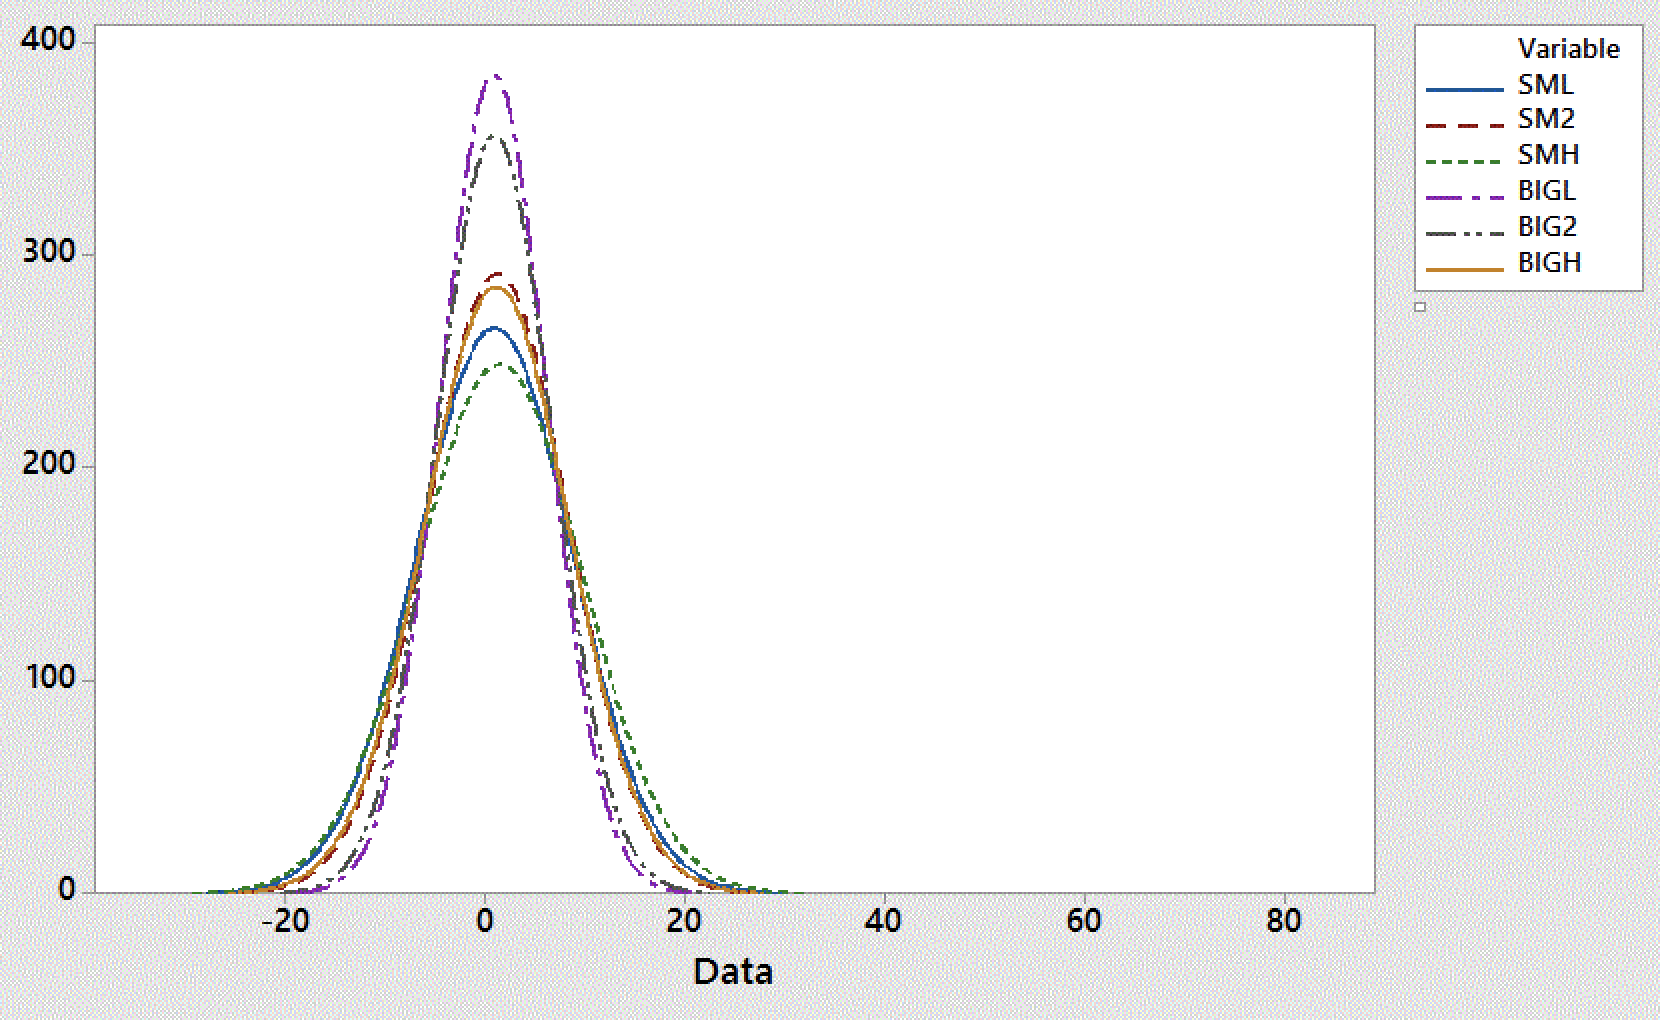
\includegraphics[width=\textwidth]{chapters/chapter_apm/figures/monreturns.png} 
   \caption{Histogram of Monthly Returns. \label{fig:monreturns}}
\end{figure}


\begin{figure}[!ht]
   \centering
   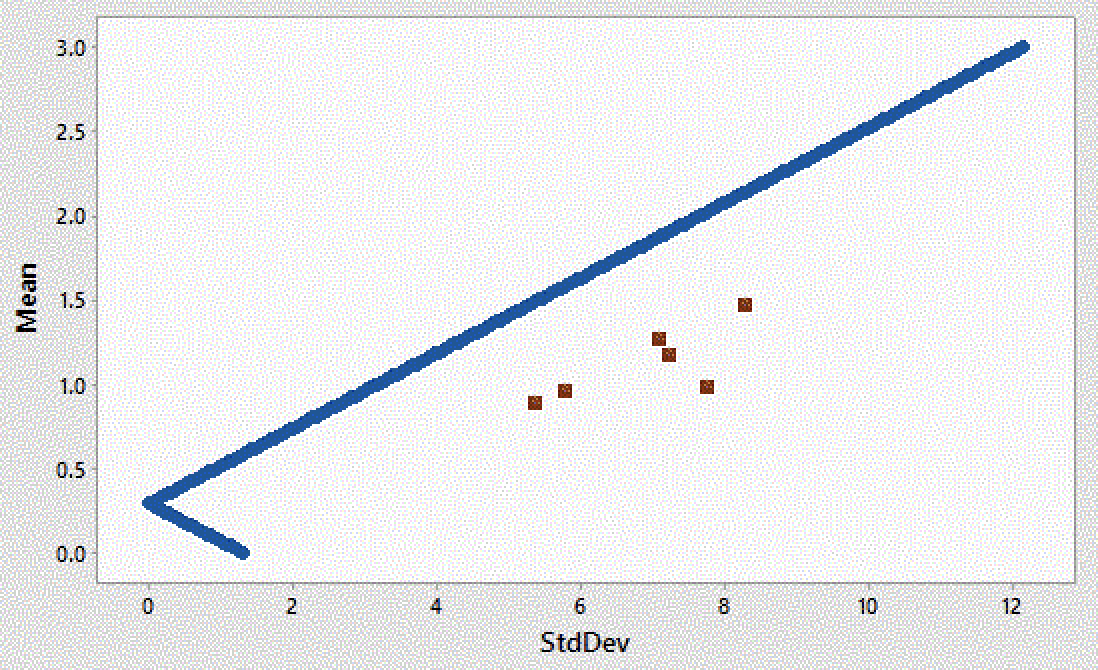
\includegraphics[width=\textwidth]{chapters/chapter_apm/figures/frontieremp.png} 
   \caption{Efficient Frontier-Empircal.\label{fig:frontemp}}
\end{figure}


\begin{table}
\centering
\caption{Descriptive statistics ($T=1036$)\label{tab:descstat}}
\begin{tabular}{lrrrrr}
Variable & Mean & StDev & Median & Skewness & Kurtosis \\
SML & 0.983 & 7.771 & 1.100 & 0.98 & 10.23 \\
SM2 & 1.271 & 7.092 & 1.530 & 1.27 & 14.51 \\
SMH & 1.472 & 8.303 & 1.660 & 2.13 & 21.64 \\
BIGL & 0.892 & 5.365 & 1.195 & $-0.13$ & 5.16 \\
BIG2 & 0.960 & 5.799 & 1.225 & 1.25 & 16.82 \\
BIGH & 1.173 & 7.243 & 1.395 & 1.53 & 18.05
\end{tabular}
\end{table}


The histogram of the portfolio returns is given in Figure~\ref{fig:frontemp}. The descriptive are stated in Table~\ref{tab:descstat}. The returns are generally positively skewed with more sharply peaked than the normal distribution. The Jarque-Bera test (Equation~\ref{eqn:2JB}) rejects the null hypothesis that returns are normally distributed. The efficient frontier with the risk-free rate using the weights in (\ref{eqn:5weff2}) along with the portfolios is plotted in Figure~\ref{fig:frontemp}, by setting $\mu^*=\hat{\mu}_m$, the average of the market portfolio. The weights for the assets are $(-1.06,1.08,0.40,0.58,-0.36,-0.32)$ and the share of the risk-free is 0.68. The scatter plot of the actual mean value versus standard deviation of the six portfolios yields the slope of 0.1471 which is larger empirical Sharpe ratio $\left(\frac{\overline{r}_m - r_f}{\hat{\sigma}_m}\right)$, 0.1147. This clearly indicates that the market portfolio is not mean-variance efficient. Note that while three portfolios (BigL, Big2, BigH) lie on the line, two others (SM2 and SMH) lie above the line. This generally implies that it is possible to outperform the empirical Markowitz portfolio. 


\begin{table}
\centering
\caption{Fama French model (estimates)\label{tab:famafrenchmodel}}
\begin{tabular}{lrrrrr}
Portfolio & Const & Market & SMB & HML & $R^2$ \\ \hline
SML & $-0.168^*$ & $1.09^*$ & $1.05^*$ & $-0.167^*$ & 0.974 \\
SM2 & 0.0625 & $0.977^*$ & $0.818^*$ & $0.702^*$ & 0.978 \\
SMH & 0.0202 & $1.03^*$ & $0.933^*$ & $0.783^*$ & 0.991 \\
BIGL & $0.077^*$ & $1.02^*$ & $-0.0965^*$ & $-0.231^*$ & 0.978 \\
BIG2 & $-0.0507$ & $0.966^*$ & $-0.122^*$ & $0.729^*$ & 0.954 \\
BIGH & $-0.112^*$ & $1.079^*$ & 0.0205 & $0.819^*$ & 0.968
\end{tabular}
\end{table}


The three known factor model results are presented in Table~\ref{tab:famafrenchmodel}. There are several conclusions that can be drawn from this table. With the three factors, the variations in the cross-sectional returns are well-captured by these factors. The coefficients of the market factors are closer to unity indicating that the six portfolios are closely aligned with the market index. But the estimates of $\alpha$ do indicate some mixed results. The value of the test statistics in (\ref{eqn:bigF}) is 5.54 which is larger than $\chi_6^2(0.05)=2.1$ and hence indicating that there should be other factors.


To identify the number of factors required to capture the total variance, we perform PCA of the covariance matrix. The Scree plot is given in Figure~\ref{fig:screeplot}. The first component is responsible for 91\% of the total variance and if three components are included we can capture 98\% of the overall variance. The first factor trading is almost proportional to unit vector indicating that it can be interpreted as a market factor. It is easy to show with three factor model, the difference between $\hat{\Sigma}$ and $\hat{B}\hat{B}'+V$ is very small. This sort of parameter reduction will become useful when we deal with large number of assets, a topic that is taken up in the next section. 


\begin{figure}[!ht]
   \centering
   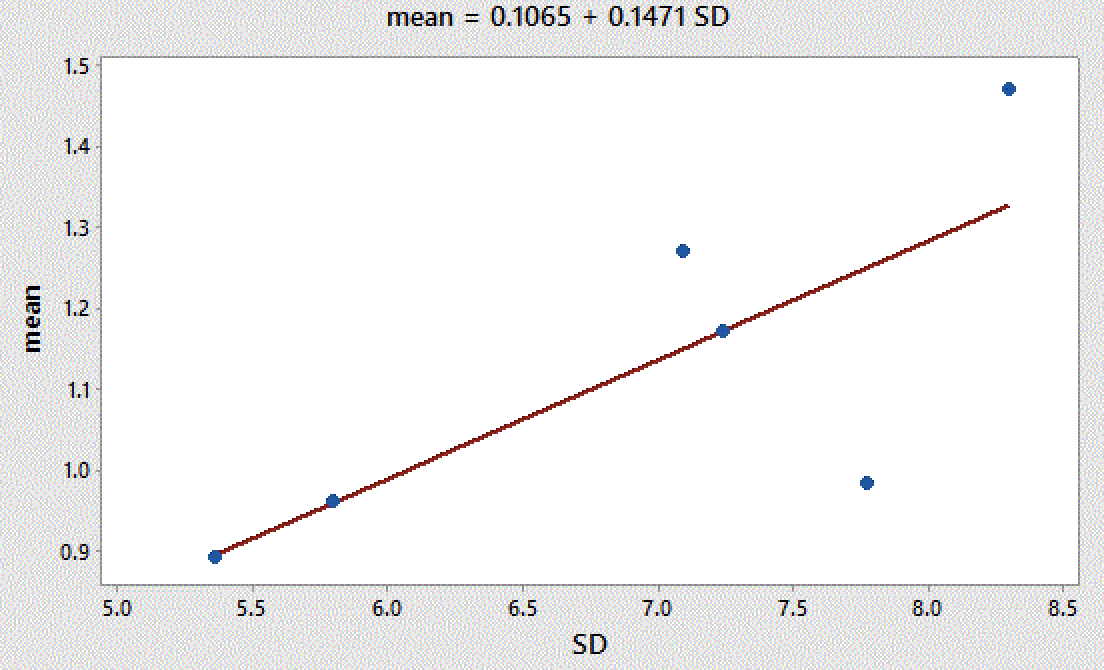
\includegraphics[width=\textwidth]{chapters/chapter_apm/figures/capmarket.png} 
   \caption{Capital Market Line.\label{fig:capmarket}}
\end{figure}


\begin{figure}[!ht]
   \centering
   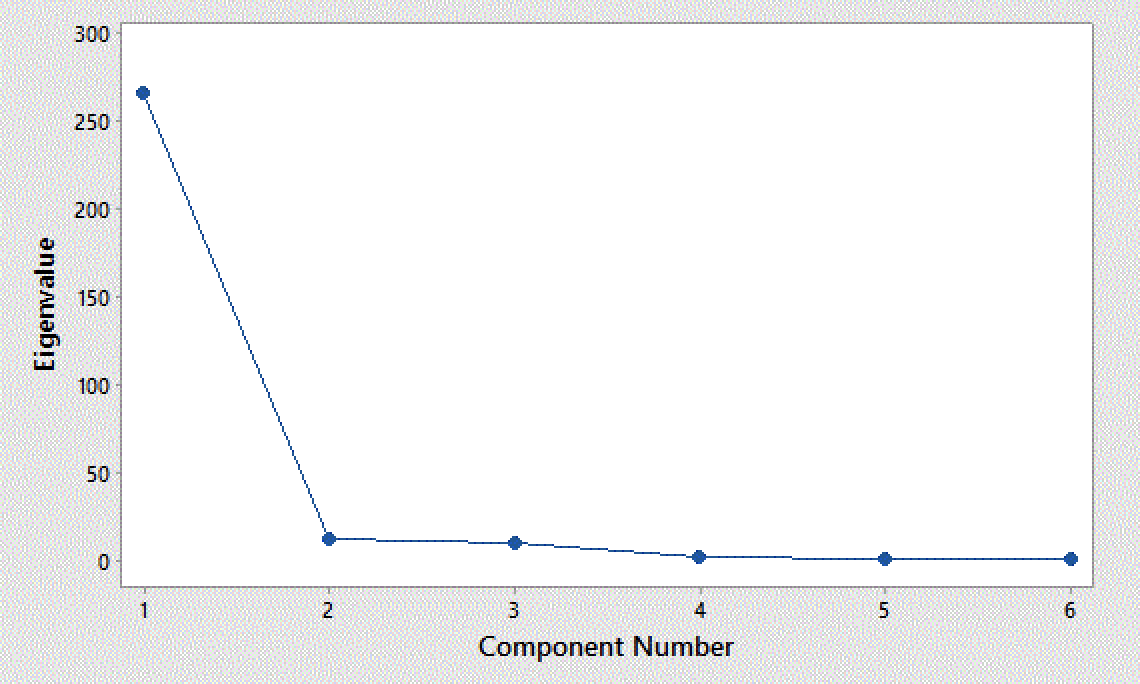
\includegraphics[width=\textwidth]{chapters/chapter_apm/figures/scree.png} 
   \caption{Scree Plot.\label{fig:screeplot}}
\end{figure}
	
	
\subsection{Summary of Models and Implications for Investing}


As the focus of this book is on trading and investing we want to summarize some main takeaways from the widely used theoretical models. Some implications of these models are listed below: \\

\noindent\textbf{One-fund Theorem:} There is a single investment of risky assets such that any efficient portfolio can be constructed as a combination of this fund and the risk-free asset. The optimal one-fund is the market fund which implies that the investor should purchase every stock which is not practical; this has given rise to the so-called index funds. \\

\noindent\textbf{Two-fund Theorem:} Two efficient portfolios (funds) can be established so that any efficient can be duplicated; all investor seeking efficient portfolios need only to invest in combinations of these two funds. \\

\noindent \textbf{No short-selling:} When the weights, $w_i$, are restricted to be positive, typically many of them tend to be zeros, by contrast with short-selling, most of the weights tend to be non-zeros. The resulting concentrated portfolios are more likely to have higher turnover rates. This has implications for the increase in trading costs. \\

\noindent\textbf{CAPM:} Recall the model is $r_i-r_f=\beta_i(r_m-r_f)+\epsilon_i$ with $\sigma_i^2=\beta_i^2\sigma^2_m + \sigma_\epsilon^2$; $\beta_i=\frac{\sigma_{im}}{\sigma_m^2}$ is the normalized version of covariance. If $\beta_i=0$, $r_i \sim r_f$ even if $\sigma_i^2$ is large. There is no risk premium; the risk that is uncorrelated with the market can be diversified away. if $\beta_i<0$, $r_i<r_f$ even if $\sigma_i^2$ is large; such an asset reduces the overall portfolio risk when it is combined with the market portfolio; they provide a form of insurance. Portfolio `Beta' is $\beta_p= \sum_{i=1}^m w_i \beta_i$. The CAPM can be used as a pricing formula. Note if the purchase price of an asset is `$P$' (known) which may be sold at `$Q$' (unknown), from CAPM, $r=\frac{Q-P}{P}=r_f+\beta(r_m-r_f)$ which results in the pricing formula
	\begin{equation}\label{eqn:pricing}
	P=\dfrac{Q}{1+r_f+\beta(r_m-r_f)}
	\end{equation}
This concept to evaluate a single asset can be extended to jointly evaluating multiple assets.


\noindent \textbf{Investment Pattern:} The minimum-variance portfolio method is likely to invest into low residual risk and low beta stocks. The CAPM model, (\ref{eqn:5ritrf}) written in the vector form leads to
	\begin{equation}\label{eqn:vectorform}
	r_t - r_f 1 = \alpha + \beta(r_{mt} - r_f) + \epsilon_t
	\end{equation}
and with the assumption that the error-covariance matrix is diagonal, the covariance matrix of the excess returns is
	\begin{equation}\label{eqn:Sigmarr}
	\Sigma_{rr}= \beta\beta' \sigma_m^2 + D
	\end{equation}	
where $D$ is diagonal with the element, $\sigma_{\epsilon i}^2$. The inverse of the covariance matrix has a simpler structure:
	\begin{equation}\label{eqn:simplestruct}
	\Sigma_{rr}^{-1}= D^{-1} - \dfrac{\sigma_m^2}{1+a} \cdot bb'
	\end{equation}	
where $a=\sigma_m^2 \cdot \sum_{i=1}^m b_i \beta_i$ and $b_i= \beta_i/\sigma_i^2$. We have shown earlier that the portfolio weights under minimum-variance is
	\begin{flalign}\label{eqn:minvariance}
	&& w&= \dfrac{\Sigma_{rr}^{-1} 1}{1' \Sigma_{rr}^{-1} 1} && \notag \\
	\text{and} && \phantom{x} & \phantom{x} && \\
	&& \sigma_{\text{MV}}^2&= \dfrac{1}{1' \Sigma_{rr}^{-1} 1} && \notag
	\end{flalign}	
Substituting (\ref{eqn:simplestruct}) in (\ref{eqn:minvariance}), notice that 
	\begin{equation}\label{eqn:wsubtitute}
	w= \sigma_{\text{MV}}^2 \left( D^{-1} 1 - \dfrac{\sigma_m^2}{1+a} \cdot bb' 1\right)
	\end{equation}
with a typical element, $w_j= \frac{\sigma_{\text{MV}}^2}{\sigma_j^2} \left(1 - \beta_j \left(\frac{\sigma_m^2}{1+a} \cdot \sum_{i=1}^m b_i \right)\right)$. It is easy to show that the second term in parenthesis above, $\frac{\sigma_m^2}{1+a} \cdot \sum_{i=1}^m b_i \sim 1$ and so
	\begin{equation}\label{eqn:wsubsecond}
	w_j= \dfrac{\sigma_{\text{MV}}^2}{\sigma_j^2} ( 1- \beta_j)
	\end{equation}
Thus when $\sigma_j^2$ is small and low $\beta_j$, $w_j$ will be large. 



\section{Statistical Underpinnings}


The implementation of the portfolio theory in practice when the means and covariances of returns are unknown has raised some challenging issues. It is a theory that applies to a single period and the choice of portfolio weights that would determine the portfolio returns for a future period. Because of uncertainty involved in the future returns the use of the estimates of the means and covariances of the returns based on the past data must be carefully evaluated. The sample average and the sample covariance matrix which are also maximum likelihood estimates under the assumptions that returns are normally distributed when plugged in, the main thesis that the combination of the assets would yield efficient portfolio does not seem to hold empirically. 


The following numerical illustration taken from Bruder, Gaussel, Richard and Roncalli (2013)~\cite{bruder} is quite telling. Consider the universe of four assets with the average return vector and the covariance matrix as given below.
	\begin{equation}\label{eqn:ovrsighat}
	\begin{split}
	\overline{r}'&= (0.05, 0.06, 0.07, 0.08) \\
	\hat{\Sigma}&=\begin{pmatrix}
	0.01 & 0.0084 & 0.0098 & 0.0105 \\
	        & 0.0144 & 0.01176 & 0.0126 \\
	        &             & 0.0156 & 0.0147 \\
	        &             &             & 0.0225
	\end{pmatrix}
	\end{split}
	\end{equation}
If the risk tolerance parameter `$\lambda$' is set at 0.1, then the resulting optimal portfolio has the following weights: $w^*=(0.2349, 0.1957, 0.1878, 0.2844)$. If the standard deviation (volatility) of the second asset increases by 3\%, the weight attached to this asset changes to $-0.1404$ and if the return of the first asset changes from 5\% to 6\%, the optimal weight goes to 0.6319 from 0.2349. The sensitivity of the efficient portfolio weights even to minor perturbations is quite obvious. 


This may be due to a number of factors. We have to keep in mind that the performance of the portfolio is related to future means and covariances of the returns. As seen from the plot of the six portfolio returns, Figure~\ref{fig:monreturns}, the distributions may not follow normal distributions. There are portfolios which are linear combinations of several individual assets and therefore individual assets can even more easily deviate from normality. Secondly, this could be result of curse of dimensionality. When `$m$' the number of assets is fairly large, the number of unknown parameters, $m(m+1)$ is also large and to estimate them accurately it requires to have a fairly large data. An extreme example would be tracking Russell index with 3000 stocks would require estimating 4.5 million covariances. Another aspect that needs to be looked into is regarding the time dependence of the returns. Under efficient market hypothesis, returns are expected to be independent; but as seen in previous chapters that there is some dependence, an anomaly exploited by the algorithms, need to be taken into account in the portfolio construction. We address these issues in this section. 


It has been shown that because of the large sampling error of the estimates, an equally weighted portfolios can perform closer to the efficient portfolio. Studies have incorporated the estimation risk via Bayesian approach and evaluated the impact of this risk on final choice of the portfolios. The exact distribution of the maximum likelihood estimators of the means and variance is well-known, but the exact distribution of the returns and the volatility of the efficient portfolio is not easy to obtain. Jobson and Korkie (1980)~\cite{jobkor} derive the asymptotic distribution and examine its properties via extensive simulations. The convergence of the sample estimates is shown to depend upon the magnitude of $T$ to $1/A^2$, where $A=1' \Sigma^{-1}\mu$, the sum of weighted averages. Generally if the covariances among the assets are relatively small but the mean returns are large, the estimators tend to perform better. In any case, good estimates of `$\mu$' and `$\Sigma$' are essential for the construction of the efficient portfolio. Michaud (1989)~\cite{michaud} suggests bootstrap methods to repeatedly resample with replacement from the observed sample of returns $(r_1,\ldots,r_m)$ and use the resulting average and the variance as the the bootstrap replications. \\


\noindent \textbf{Shrinkage and Bayesian Methods:} The shrinkage methods follow the same optimization criterion but impose a penalty on the size of the coefficients. For example, we can add following additional constraints to (\ref{eqn:5opt}):
	\begin{equation}\label{eqn:addconstraint}
	\begin{split}
	\text{Ridge: }& \sum_{i=1}^m w_i^2 \leq w \\
	\text{Lasso: }&\sum_{i=1}^m |w_i| \leq w
	\end{split}
	\end{equation}
Both procedures can be unified as, $\sum_{i=1}^m |w_i|^q \leq w$ for $1 \leq q \leq 2$. As it has been shown that these methods yield estimates that are Bayes estimates with different priors, we will now discuss Bayesian approach. 


The Bayesian approach combines the prior distribution and the likelihood to obtain posterior distribution of the unknown parameters. Usually the mode of this distribution is taken as a reasonable estimate. In a influential paper, Black and Litterman (1992)~\cite{blacklit} describe the need for Bayesian approach. The straight solution to (\ref{eqn:5opt}) almost always results in large short positions in many assets which would increase the trading costs. If the weights are restricted to be positive the solution results in zero weights for many assets and large weights in the assets with small capitalizations. The results generally are not reasonable mainly due to poor estimate of expected future returns. In practice, investors augment their views using their prior experience and their intuition to forecast the likely returns based on other asset related data. The Bayes Theorem in a natural way combines these two aspects. The details that follow are from Lai, Xin and Chen (2011)~\cite{laixingchen} and we will comment on the practical implementation issues after presenting mathematical results. 


The model begins with the following distributions:
	\begin{equation}\label{eqn:5distributions}
	r_t \sim N(\mu,\Sigma), \enskip \mu \big| \Sigma \sim N(\nu, \Sigma/\kappa) \text{ and } \Sigma \sim IW_m(\psi,n_0)
	\end{equation}
where $IW_m(\psi,n_0)$ is the inverted Wishart with `$n_0$' degrees of freedom with $E(\Sigma)=\psi/(n_0-m-1)$. These prior are known as conjugate priors as their functional forms closely match the likelihood functional form. When the degree of freedom `$\kappa$' goes to zero, the prior is non-informative. The posterior means are:
	\begin{equation}\label{eqn:5posterior}
	\begin{split}
	\hat{\mu}&= \dfrac{\kappa}{T+\kappa} \cdot \nu + \dfrac{T}{T+\kappa} \overline{r} \\
	\hat{\Sigma}&= \dfrac{\psi}{T+n_0-m-1} + \dfrac{T}{T+n_0-m-1} \cdot \left\{s+ \dfrac{\kappa}{T+\kappa} (\overline{r}-\nu)(\overline{r}-\nu)' \right\}
	\end{split}
	\end{equation}
where $S=\frac{1}{T} \sum_{t=1}^T (r_t-\overline{r})(r_t-\overline{r})'$, the residual covariance matrix. If `$\kappa$' and `$n_0$' are taken to be large, it implies that the investor puts more emphasis on priors. To use (\ref{eqn:5posterior}), the investor has to specify these values. 


Black and Litterman (1992)~\cite{blacklit} propose shrinking the prior estimate of $\mu$ to a vector `$\pi$' representing excess equilibrium returns such as the one implied by CAPM which is termed as the return on the global market. Thus
	\begin{equation}\label{eqn:bigpi}
	\pi = \dfrac{\mu_m-r_f}{\sigma_m^2} \cdot \Sigma \cdot w_m
	\end{equation}
where $w_m$ are the weights on the global market and $\sigma_m^2$ is the variance of the rate of return on the global market. To get the posterior distribution of $\mu \big| \pi$ via Bayes Theorem, as mentioned in Satchell and Snowcraft (2000)~\cite{snow}, the approach by Black and Litterman (1992)~\cite{blacklit}  was to place this in a tractable form that investors can operationalize. Assume that $k \times m$ matrix $P$ represents investor's beliefs, then $P \mu \sim N(q,\Omega)$, where `$\Omega$' is diagonal. The parameters `$q$' and `$\Omega$' are known as hyperparameters. Also it is assumed that $\pi \big| \mu \sim N(\mu,\tau \Sigma)$, where $\tau$ is a scaling factor. Thus the p.d.f. of `$\mu$' is given as $\mu \big| \pi \sim N(\hat{\mu}^{\text{BL}}, \hat{\Sigma}^{\text{BL}})$, where 
	\begin{flalign}\label{eqn:bleq}
	&& \hat{\mu}^{\text{BL}}&= (\hat{\Sigma}^{\text{BL}})^{-1} [ (\tau \Sigma)^{-1}\pi + P' \Omega^{-1}q] && \notag \\
	\text{and} && \phantom{x} & \phantom{x} && \\
	&& \hat{\Sigma}^{\text{BL}}&= (\tau \Sigma)^{-1} + P' \Omega^{-1}P && \notag
	\end{flalign}
For various interesting practical applications, see Satchell and Snowcraft (2000)~\cite{snow}. But the requirement for subjective judgements makes it difficult to use Black-Litterman model in asset management practice. 


It has been noted in the literature that estimating the expected returns using the past returns fails to account for likely changes in the level of market risk. Merton (1980)~\cite{merton} based on a detailed exploratory study concludes that the investors should recognize that the expected market return in excess of risk free return should be positive and that there is heteroscedasticity in the realized returns. It must be noted that the price series is random walk and therefore with shifting means, the successive differences (essentially the returns) can exhibit different levels of variances. Recent focus has been on the improved estimation of the covariance matrix, $\Sigma$. As the sample covariance matrix with $m(m+1)/2$ elements requires substantially large `$T$' for estimation, alternatives for a structural covariance matrix with fewer parameters are proposed. There are all in the same spirit of shrinkage estimators:
	\begin{equation}\label{eqn:5HatSigma}
	\hat{\Sigma}= \alpha s_0 + (1-\alpha)s
	\end{equation}
where `$\alpha$' is called a shrinkage constant and `$s_0$' matrix is restricted to have only a few `freer' elements. With the CAPM model that leads to covariance structure, (\ref{eqn:Sigmarr}), the resulting covariance matrix which is the sum of a diagonal matrix and a matrix of rank one, will have only `$2m$' independent elements that need to be estimated. Ledoit and Wolf (2003)~\cite{wolf} describe a procedure to arrive at the estimate of $\alpha$ in (\ref{eqn:5HatSigma}) which we briefly describe below. 


Minimizing the following risk function,
	\begin{equation}\label{eqn:ralpha}
	R(\alpha)= \sum_{i=1}^m \sum_{j=1}^m E(\alpha s_{ij}^0 + (1-\alpha) s_{ij} - \sigma_{ij})^2
	\end{equation}
we arrive at `$\alpha$' as
	\begin{equation}\label{eqn:bigalpha}
	\alpha^*= \dfrac{\sum_i \sum_{j} \left[ \Var(s_{ij}) - \Cov(s_{ij}^0, s_{ij}) \right]}{\sum_i \sum_j \left[ \Var(s_{ij}^0 - s_{ij}) + (\phi_{ij} - \sigma_{ij})^2 \right]}
	\end{equation}
where $\phi_{ij}=E[\alpha s_{ij}^0 + (1-\alpha)s_{ij}]$. It is further shown that
	\begin{equation}\label{eqn:alphastarsim}
	\alpha^* \sim \dfrac{1}{T} \cdot \dfrac{\pi - \rho}{\gamma}
	\end{equation}
where $\pi= \sum_i \sum_j \text{Asy}\Var(\sqrt{T}s_{ij})$, $\rho=\sum_i \sum_j \text{Asy}\Cov(\sqrt{T}\,s_{ij}^0, s_{ij})$ and $\gamma=\sum_i \sum_j (\phi_{ij} - \sigma_{ij})^2$. Note that with CAPM specification which can be taken as a single index model, the `$\gamma$' quantity represents the misspecification of the single index. 


Fan, Fan and Lv (2008)~\cite{fansq} consider high dimensional covariance matrix estimation via factor model (\ref{eqn:arbrit}). The multifactor model generally captures well the cross-sectional variations and thus the number of parameters that need to be estimated can be significantly reduced. It is possible that the number of factors `$n$' can grow with the number of assets, `$m$', and the sample period, `$T$'. Comparing $\hat{\Sigma}_{rr}= \hat{B} \hat{\Omega} \hat{B}' + \hat{V}$ in (\ref{eqn:covdouble}) with the sample covariance matrix of the returns, `$S$', it is shown that the former performs better if the underlying factor model is true. In calculations that involve the inverse of the covariance matrix, such as the calculation of portfolio weights, factor model based estimates tend to perform better but it does not make a difference in the actual risk calculation ($\hat{w}' \hat{\Sigma} \hat{w}$), which involves the estimate of the covariance matrix. Recent studies have focused on proving bounds on the risk; the calculations are somewhat complicated as they involve estimates of the weight vector as well as the estimates of the covariance matrix. See Fan, Han, Liu and Vickers (2016)~\cite{vickers} and the references therein. 



\subsection{Portfolio Allocation Using Regularization}


It is noted that the poor performance of Markowitz's conceptual framework is due to the structure of the optimization problem. It is an ill-conditioned inverse problem as the solution requires the inverse of the covariance matrix that may involve highly correlated securities. A number of regularization procedures have been proposed in the literature to address the instability in the solution and we present a few of them here. \\


\noindent \textbf{The $\mathbf{L_2}$ Constraint:} This is also known as ridge constraint that imposes the penalty on the size of the estimates as given in (\ref{eqn:addconstraint}). The problem is defined as follows:
	\begin{equation}\label{eqn:minwsum}
	\min_w w' \Sigma w \ni w' \mu=\mu^*, w'\mu=1 \text{ and }\sum_{i=1}^m w_i^2 \leq w_0
	\end{equation}
when there are many correlated assets, the weights are poorly determined and can exhibit high variance. A large positive weight for an asset can be canceled by a large negative weight for the correlated asset. The size constraint added in (\ref{eqn:minwsum}) can address this issue. If the added constraint has the associated Lagrangian multiplier, $\gamma^*$, the solution in (\ref{eqn:5weff}) is modified by replacing $\Sigma$ by ($\Sigma + \gamma^* I_m$). The solution adds a positive constant to smaller eigenvalues of possibly a singular matrix, $\Sigma$. Observe that the eigen decomposition of $\Sigma= V \Lambda V'$ essentially gives us the principal components of the asset universe considered for the formation of the portfolio. The optimization can also be extended to accommodating to mimic a target portfolio with weights $w^*$. The set-up would be the same except for the last size constraint is replaced by
	\begin{equation}\label{eqn:wminwstar}
	(w-w^*)' A(w-w^*) \leq w_0
	\end{equation}
If `$\lambda$' and `$\gamma$' are the Lagrangian multipliers associated with the mean specification constraint in (\ref{eqn:wminwstar}) and the constraint above, the solution is
	\begin{equation}\label{eqn:hatwlambdagamma}
	\hat{w}(\lambda,\gamma)=(\hat{\Sigma} + \gamma A)^{-1} (\lambda \hat{\mu} + \gamma A w_0)
	\end{equation}
which results from shrinking both the mean vector and the covariance matrix. \\

\noindent \textbf{The $\mathbf{L_1}$ Constraint:} The method popularly called as LASSO (least absolute shrinkage and selection operator) is a shrinkage method like the ridge but there are some important differences. The problem can be stated as follows:
	\begin{equation}\label{eqn:minwsum2}
	\min_w w'\Sigma w \ni w'\mu=\mu^*, w'\mu=1 \text{ and } \sum_{i=1}^m |w_i| \leq w_0
	\end{equation}
The added constraint in (\ref{eqn:minwsum2}) leads to nonlinear solutions and no explicit solution as with ridge penalty is possible. The numerical solutions are obtained via quadratic programming.


Both $L_1$ and $L_2$ constraint versions yield solutions that can be justified as Bayes with different priors. The LASSO method produces sparse solution that is easy to interpret. Sparser solution in the portfolio context means lower transaction costs when the portfolios are rebalanced. A convenient way to solve these optimization problems is to formulate the original set-up in (\ref{eqn:5opt}) in the regression framework; this will help to borrow regularization ideas used in the general area of multivariate regression. Observe that $\Sigma=E(r_tr_t') - \mu\mu'$ and thus the minimization problem is equivalent to (in the sample version)
	\begin{equation}\label{eqn:hatwarg}
	\hat{w}= \text{arg }\min_w \dfrac{1}{T} \| \mu^*1_T - R'w\|_2 \ni w'\hat{\mu} = \mu^*, w'1_m=1
	\end{equation}
Here $R$ is the $m\times T$ matrix of the row returns and $\hat{\mu}=\frac{1}{T}\sum_{t=1}^T r_t$. The regularization constraint in (\ref{eqn:minwsum2}) when added to (\ref{eqn:hatwarg}) results in the following optimization problem:
	\begin{equation}\label{eqn:anotherhatwargmin}
	\hat{w}^{(\tau)}= \text{arg } \min_w [ \|\mu^* 1_T - R'w\|_2 + \tau\|w\|_1] \ni w' \hat{\mu} = \mu^*, w'1_m=1
	\end{equation}
As stated in Brodie, Daubechies, De Mol, Giannone and Loris (2009)~\cite{brodic} adding the $l_1$-constraint results in several useful advantages. In addition to introducing sparsity that is helpful for managing large portfolios, the procedure provides a framework for regulating the amount of shorting which can be a proxy for the transaction costs. More importantly it provides a solution that is more stable which was a main concern as small perturbations in the estimates of $\mu$ and $\Sigma$ can lead to very different solutions.


The algorithm that is most convenient to solve (\ref{eqn:anotherhatwargmin}) is Least Angle Regression (LAR) developed in Efron, Hastie, Johnstone and Tibshirani (2004)~\cite{efron}. It starts with a large value of `$\tau$' and as `$\tau$' decreases the optimal solution, $\hat{w}^{(\tau)}$, changes in a piecewise linear fashion and thus it is only essential to find critical points where the slope changes. More relevant details can be found in Brodic et al. (2009)~\cite{brodic}. The LASSO procedure was evaluated using Fama-French 100 portfolios sorted by size and book-to-market as the universe. The efficient portfolio was constructed on a rolling basis using the monthly data for five years and its performance is evaluated in the following year. It is concluded, see Brodie et al. (2009; Figure 2)~\cite{brodic}, that optimal sparse portfolios that allow short portfolios tend to outperform both optimal no-short-positions portfolio and the na\"ive evenly weighted portfolio. 



\subsection{Portfolio Strategies: Some General Findings}



The following wisdom advocated by Rabbi Isaac bar Aha that ``one should always divide his wealth into three parts: a third in land, a third in merchandise and a third ready to hand'', the equal division among the assets has been tested out in the case of equity allocation as well. Although this diversification strategy appears to be na\"ive because it is based on neither any theory nor any data, has done relatively well. DeMiguel, Garlappi and Uppal (2009)~\cite{demig} compare this na\"ive strategy with other theory-based strategies that were discussed in earlier sections in terms of its performance using various data sets. The summary of their findings is worth noting: ``\dots of the strategies from the optimizing models, there is no single strategy that dominates the $1/N$ strategy in terms of Sharpe ratio. In general, $1/N$ strategy has Sharpe ratios that are higher \dots relative to the constrained policies which in turn have Sharpe ratios that are higher than those for the unconstrained policies.''


The na\"ive portfolio has also very low turnover. In addition to keeping na\"ive portfolio as  a benchmark, a practical implication is that the estimation of the moments of asset returns needs improvement using other information based on asset characteristics. \\


\noindent \textbf{Combination of Strategies:} Tu and Zhou (2011)~\cite{jtu} combine the rules based on Markowitz Theory with the na\"ive strategy to obtain new portfolio rules that can perform uniformly better. The combination can be interpreted as a shrinkage estimator, shrinking toward the na\"ive estimator. The linear combination
	\begin{equation}\label{eqn:lincomb}
	\hat{w}_c = \delta \hat{w} + (1-\delta) w_N
	\end{equation}
where $\hat{w}$ is the weights that come from variations of efficient portfolios and $w_N$ has all its elements equal. With the criterion of minimizing the loss function, 
	\begin{equation}\label{eqn:lossfun}
	L(w^*,\hat{w}_c)= U(w^*) - E[U(\hat{w}_c)]
	\end{equation}
where $U(\cdot)$ is the expected utility, the combination coefficient $\delta$, is obtained. This strategy was tested out using the same data as in DeMiguel et al. (2009)~\cite{demig} and generally the combination rules perform well. \\


\noindent\textbf{Familiarity:} It has been advocated by many economists and practitioners such as Warren Buffet that investors should focus on a few stocks that they are familiar with rather than a wide scale of diversification. Boyle, Garlappi, Uppal and Wang (2012)~\cite{bguwang} develop a theoretical framework to answer some relevant questions related to familiarity and diversification. Writing the return as sum of components, systematic and idiosyncratic,
	\begin{equation}\label{eqn:rirsui}
	r_i = r_s + u_i \quad\quad i=1,2,\ldots,m
	\end{equation}
the utility function in (\ref{eqn:utility}) is modified to take into account the investors familiarity with some assets. This is done via the assumption that the investor is ambiguous about the mean, $\mu$, but has perfect knowledge about $\sigma$. This information alters the criterion in (\ref{eqn:5maxu}) as,
	\begin{equation}\label{eqn:maxminwmu}
	\max_w \min_\mu \left(w'\mu - \frac{\lambda}{2} \cdot w' \Sigma w \right)\enskip \ni \enskip\dfrac{(\mu-\hat{\mu})^2}{\sigma_{\hat{\mu}}^2} \leq \alpha_i^2, \quad i=1,2,\ldots,m
	\end{equation}
where $\sigma_{\hat{\mu}}^2= (\sigma_s^2+\sigma_u^2)/T$. Two key quantities that play important roles are the level of ambiguity `$\alpha_i$' and the inverse coefficient of variation, $\hat{\mu}/\sigma_{\hat{\mu}}$. Some conclusions from this study are
\begin{enumerate}[--]
\item When ambiguity is present, the investor tends to hold disproportionate (to Markowitz allocation) amount in the familiar assets.
\item When ambiguity is present, the number of assets tends to be smaller.
\end{enumerate}


Huberman (2001)~\cite{Hub} provides several instances of investment in the familiar options rather than choices that lead to efficient outcome. Workers generally tend to choose their employers stock as they probably think that they know about their behavior and may believe they have information that the market does not have. Thus various examples are provided that indicate that although investment in the familiar contradicts the advice to diversify. This adds a dimension to the traditional risk-return formulation that one has to recognize. \\


\noindent\textbf{Large Portfolio Selection with Exposure Constraints:} Several techniques have been discussed in this section to reduce the sensitivity of the optimal portfolio weights to uncertainty in the inputs, such as the mean returns and the covariance matrix of returns. Generally these techniques are not adequate to address the effect of estimation errors that accumulate due to large portfolio size. Jagannathan and Ma (2003)~\cite{jagma} impose no short-sales constraints as well as upper bounds on portfolio weights as commonly imposed by practitioners. The empirical evidence indicates that simply imposing upper bounds does not lead to significant improvement in the out-of-sample performance. For an estimated covariance matrix, $S$, the formulation of the model is as follows:
	\begin{equation}\label{eqn:estcovmat}
	\min_w w'Sw \enskip \ni \enskip w'1=1, \enskip 0\leq w_i \leq \tilde{w} \enskip\text{ for }i=1,2,\ldots,m
	\end{equation}
Note the variation in its formulation; no expectation on the average return of the portfolio as in Markowitz set-up is specified. Fan, Zhang and Yu (2012)~\cite{fanzhanyu} argue that the resulting optimal portfolio, although performs well, it is not diversified enough. 


Defining the total proportions of long and short positions by $w^+=(\|w\|_1+1)/2$ and $w^-=(\|w\|_1-1)/2$, we have $w^+ + w^-= \|w\|_1$ and $w^+ - w^- =1$. The optimization problem is stated as,
	\begin{equation} \label{eqn:optproblem}
	\max_w E[U(w'r)] \enskip \ni \enskip w'1=1, \|w\|_1 \leq C \text{ and } Aw=a
	\end{equation}
Here $U(\cdot)$ is a utility function and the extra-constraints $Aw=a$ can capture allocations to various sectors. But the key added constraint, $\|w\|_1 \leq C$ can accommodate from no short sales ($C=1$) to unrestricted sales ($C=\infty$) constraints. The solution to (\ref{eqn:optproblem}) can be obtained via quadratic programming. Fan et al. (2012)~\cite{fanzhanyu} advocate data-driven choice of `$C$' via minimizing the risk for a sample learning period. Using select 600 stocks from the pool of stocks that constitute Russell 3000, the constructed portfolios tend to perform well for $C \sim 2$. 


\section{Dynamic Portfolio Selection}


The static Markowitz framework, as discussed in the last section, is not realistic for practical implication. Dynamic approaches that have been discussed in the literature will be presented here briefly. The single period optimization problem can be formulated as,
	\begin{equation}\label{eqn:periodopt}
	\max_{w_t} E_t \left[ w_t' r_{t+1} - \frac{\gamma}{2}(w_t' r_{t+1})^2\right]
	\end{equation} 
which results in the optimal solution,
	\begin{equation}\label{eqn:periodoptimal}
	w_t= w= \frac{1}{\gamma} \cdot E\left[r_{t+1} r_{t+1}']^{-1} E[r_{t+1}\right]
	\end{equation}	
that can be estimated using the sample counterpart. Here $r_{t+1}$ is the excess returns $R_{t+1} - R_t^f$. It is assumed here that the returns are independent and identically distributed. Brandt and Santa-Clara (2006)~\cite{bransc} extend the above set-up to multiperiods. Simply stated the two-period mean-variance objective function is,
	\begin{equation}\label{eqn:twoperiodmv}
	\max E_t \left[ r^p_{t \to t+2} - \frac{\gamma}{2} ( r^p_{t \to t+2}\right]
	\end{equation}
where the excess return for the two period investment strategy,
	\begin{equation}\label{eqn:twoperexcess}
	r^p_{t \to t+2} = (R_t^f + w_t' r_{t+1}) ( R^f_{t+1} + w_{t+1}' r_{t+2}) - R_t^f R_{t+1}^f
	\end{equation}	
It can be seen that the above expression can be written as 
	\begin{equation}\label{eqn:rewritten}
	r^p_{t \to t+2} = w_t' (r_{t+1} R_{t+1}^f) + w_{t+1}' (r_{t+2}R_t^f) + (w_t' r_{t+1})(w_{t+1}' r_{t+2})
	\end{equation}
with the first two terms denoting excess returns from investing in the risk free asset in the first period and in the risky asset in the second period and vice versa. The third term that captures the effect of compounding is of smaller magnitude. Ignoring that term results in the optimal portfolio  weights,
	\begin{equation}\label{eqn:optimalweights}
	w= \frac{1}{\gamma} E\left[ r^{p}_{t \to t+2} {r'}^p_{t\to t+2} \right] E[r^{p}_{t \to t+2}]
	\end{equation}
The solution reflects the the choice between holdings the risky assets in the first period only and holding them in the second period only and thus is termed as ``timing portfolios''. The above result can be extended to any number of periods. \\


\noindent\textbf{Conditioning Information in Portofolio Construction:} It has been debated that the portfolio managers may use conditioning information they have about assets in forming the portfolios, not simply using the mean and variance of the past returns. Thus the managers' conditionally efficient portfolios may not appear efficient to the investor with no knowledge of that information. Ferson and Siegel (2001)~\cite{fersie} study the properties of unconditional minimum-variance portfolios when the conditioning information is present. ``For extreme signals about the returns of risky assets, the efficient solution requires a conservative response.'' Managers reduce risk by taking a small position in the risky asset while keeping the same level of portfolio performance. In its basic formulation, assuming that the investment alternatives are a risky asset and risk-free return, with $w(\tilde{S})$---the proportion invested in the risky-asset, the portfolio return and the variance are: 
	\begin{flalign}\label{eqn:preturnvar}
	&& \mu_p&= E[r_f+w(\tilde{S})(r_t-r_f)] && \notag \\
	\text{and} && \phantom{x} & \phantom{x} && \\
	&& \sigma_p^2&= E[(w(\tilde{S})(r_t - r_f))^2] - (\mu_p - r_f)^2 && \notag
	\end{flalign}
Here $\tilde{S}$ is the observed signal and $w(\tilde{S})$ is a function of that signal that the manager considers at the time of allocation. The minimization criterion leads to the following weight for the risk asset:
	\begin{equation}\label{eqn:riskyassetweight}
	w(\tilde{S})= \dfrac{\mu_p - r_f}{C} \left( \dfrac{\mu(\tilde{S}) - r_f}{(\mu(\tilde{S} - r_f)^2 + \sigma^2_\epsilon(\tilde{S})} \right)
	\end{equation}
where ${C= E\left[ \frac{(\mu(\tilde{S}) - r_f)^2}{(\mu(\tilde{S}) - r_f)^2 + \sigma^2_\epsilon(\tilde{S})} \right]}$ and the minimized variance is ${\sigma_p^2=(\mu_p-r_f)^2\left(\dfrac{1}{C} - 1\right)}$. Here $\sigma_\epsilon^2(\tilde{S})$ is the conditional variance given the signal. Note when this is zero, which signifies that there is no conditional information, $w(\tilde{S})=w=(\mu_p-r_f)/(\mu-r_f)$, that is the result of Markowitz theorem. The above results can be easily extended to multiple risky asset scenario.


To implement this idea, we assume that the weight vector is a linear function of `$k$' state variables:
	\begin{equation}\label{eqn:statevar}
	w_t= \theta z_t
	\end{equation}
and the maximization criterion in (\ref{eqn:periodopt}) can be modified as,
	\begin{equation}\label{eqn:prevmodified}
	\max_\theta E_t\left[(\theta z_t)' r_{t+1} - \frac{\gamma}{2}(\theta z_t)' r_{t+1} r_{t+1}' (\theta z_t)\right]
	\end{equation}
Denoting $\overline{r}_{t+1}=z_t \otimes r_{t+1}$ and $\tilde{w}=\text{vec}(\theta)$, we can obtain the optimal solution as,
	\begin{equation}\label{eqn:modifiedsolution}
	\begin{split}
	\tilde{w}&=\frac{1}{\gamma} E[\tilde{r}_{t+1} \tilde{r}_{t+1}']^{-1} E(\tilde{r}_{t+1}) \\
	&=\frac{1}{\gamma} E[(z_t z_t' \otimes (r_{t+1}r_{t+1}')]^{-1} E[z_t \otimes r_{t-1}]
	\end{split}
	\end{equation}
Here $\otimes$ is meant for a Kronecker product. Brandt and Santa-Clara (2006)~\cite{bransc} also show how both single period and multi-period problems can be formulated as the constrained VAR. 


Using the established evidence from the literature that market returns can be predicted by conditioning on divided-price ratio, short-term interest rate, term spread and credit spread, to study the market returns for both stocks and bonds, the authors evaluate the conditional and unconditional policies at monthly, quarterly and annual holding periods, with the value of $\gamma=5$. Some general conclusions are:
	\begin{enumerate}[--]
	\item Conditional policies are quite sensitive to state variables. Because of the predictability of returns, conditional policies allow for the investor to be more aggressive on average. Sharpe ratios are generally higher for conditional policies.
	\item Results are less pronounced for the larger holding periods. Conditional policies can be very different at different time frequencies.
	\item The above stated conclusions hold for multiperiod portfolio policies as well with monthly rebalancing. 
	\end{enumerate}


\section{Portfolio Tracking and Rebalancing}


The proportions of capital allocated to various assets can change due to their performances and investors risk aversion or objectives also can change over time. Thus investors often engage in portfolio rebalancing to keep the portfolio on target risk exposure and exploit the market opportunities to enhance returns in the long run. First we formulate the problem with constraints and then present the results of some empirical studies.


The portfolio returns ($r_t$) are generally compared with some index returns ($I_t$); the excess return ($ER$) are the tracking error ($TE$) are defined as follows:
	\begin{equation}\label{eqn:excesstrack}
	\begin{split}
	ER&= \dfrac{1}{T} \sum_{t=1}^T (r_t - I_t) \\
	TE&= \dfrac{1}{T} \sum_{t=1}^T (r_T - I_t)^2
	\end{split}
	\end{equation}
The optimization function is to minimize $\lambda\sqrt{TE} - (1-\lambda)ER$, via the choice of the portfolio weights. Another optimization set-up is to balance between tracking error and transaction costs. Let $x=w-w_0$, where `$w_0$' is the current portfolio weights and `$w$' is the target weights; the problem with constraints can be stated as:
	\begin{equation}\label{eqn:constraintprob}
	\min_w (w-w_0) \Omega (w-w_0) \enskip \ni w'1=1
	\end{equation}
subject to the following constraints:
	\begin{equation}\label{eqn:constraintlist}
	\begin{split}
	&w \geq 0 \enskip \text{long only} \\
	&\sum |x_i| \leq u \enskip \text{turn-over} \\
	&\sum_{i=1}^m \beta_{ik} w_i \leq u_k \enskip \text{maximum exposure to a factor} \\
	&l_i \leq w_i \leq u_i \enskip \text{holding}
	\end{split}
	\end{equation}
Note the criterion in (\ref{eqn:constraintprob}) can also be taken as a version of tracking error. 


Some practical implementation ideas are discussed in Pachmanova and Fabozzi (2014)~\cite{pachfab}. In addition to na\"ive allocation strategy discussed earlier in this chapter, other ad-hoc methods simply imitate the composition of some market indices such as S\&P 500 that weighs stocks by their market capitalizations or Dow-Jones that weighs stocks by their prices. To imitate, select the stocks with the largest weights in the benchmark. Other methods include stratification of benchmarks into groups and select stocks from each group that ensures diversification. The groups can be industry-based or if it is based on past performance, the selected assets are called basis assets. The difference between the original allocation model and the rebalancing models can be due to change in the objectives and also change in the transaction costs and taxes. If a manager wants to move toward higher alpha, the restriction on the tracking error should be added to (\ref{eqn:constraintlist}). Like other calculations related to portfolio management, the rebalancing also involves backward-looking estimates. To reflect the future more accurately, managers should arrive at forward-looking estimates of tracking error using conditioning arguments given in the earlier section. \\


\noindent\textbf{Transaction Costs:} Bid-ask spreads, brokerage fees, taxes and the price impact on trading are covered in Chapter 7. Here we present some observations related to trading costs as noted in the literature. Defining the turnover as,
	\begin{equation}\label{eqn:turnover}
	\mathcal{T}= \sum_{i=1}^m |w_i - w_{0i}| = \sum_{i=1}^m \tau_i
	\end{equation}
and the costs of rebalancing is
	\begin{equation}\label{eqn:rebalance}
	C= \sum_{i=1}^m k_i \tau_i
	\end{equation}
Note $w_{0i}=\frac{w_i r_i}{\sum w_i r_i}$ and $\tau_i= \left|\frac{w_i(r_i-r_{0i})}{\sum w_ir_i}\right|$ and thus a key term here is $r_i-r_{0i}$, the difference between the actual and target return for asset `$i$'. Kourtis (2014)~\cite{kourtis} studies the distribution of $\tau$ and $C$ under the na\"ive allocation strategy. Denoting $r^p=\sum w_ir_i$ the portfolio return, the distribution of $\tau_i$ depends on $(r_i-r_{0i})/r^p$, the ratio of excess return to the portfolio return. A general formulation that accounts for the transaction cost is
	\begin{equation}\label{eqn:transcostaccount}
	\min_w \delta (w-w_0)' \Omega(w-w_0) + \sum_{i=1}^m k_i E[\tau_i (r_{i,}w)]
	\end{equation}
with the controlling parameter, $\delta$, on the tracking error. By explicitly incorporating the trading cost in the criterion, it is shown that the total cost of transaction is reduced.


Moorman (2014)~\cite{moorman} considers three portfolio strategies: a levered-momentum strategy, a zero-cost-decile momentum strategy and equally-weighted na\"ive strategy. Because the momentum strategies adapt to changing market conditions swiftly requires frequent rebalancing and can reveal the drawbacks of any method to reduce transaction costs. First there is a no-trade region where the distance between target and the current weight is not significant. Write the rebalanced weight as,
	\begin{equation}\label{eqn:rebalanceweight}
	w_t^*= \alpha_t w_{0t} + (1-\alpha_t)w_t
	\end{equation}
where `$\alpha_t$' is the rate of rebalancing; if $\alpha_t=1$, then there is no rebalancing. It is easily seen that the current month's unbalanced weights are related to prior month's rebalanced weights as,
	\begin{equation}\label{eqn:priorrebalanced}
	w_{0t}= w_{t-1}^* \left(\dfrac{1-r_t}{1+r_{pt}}\right)
	\end{equation}
where $r_{pt}$ is the before-transaction cost return on the portfolio. Note
	\begin{equation}\label{eqn:transnote}
	r_{pt}= \sum_{i=1}^{N_t} w_{it}^* r_{it} - c_{it} |w_{it}^* - w_{0t}|
	\end{equation}
where $c_{it}$ is the cost of transaction. The `$\alpha$' is chosen using the following objective function that results from constant relative risk aversion utility:
	\begin{equation}\label{eqn:objectivefun}
	\max_\alpha \dfrac{1}{T} \sum_{t=0}^{T-1} \dfrac{(1+r_{pt+1})^{1-\gamma}}{1-\gamma}
	\end{equation}
where `$\gamma$' is the coefficient of relative risk-aversion. The parameter `$\alpha$' is chosen via grid search, outside no-trade zone. An empirical investigation of various distance and rebalancing methods reveal that transaction cost reduction is most successful for the lowered momentum and equally-weighted market portfolios but more difficult for the momentum portfolios because of higher turnover. 



\section{Transaction Costs, Shorting and Liquidity Constraints}


It is clear, based on the discussion in this chapter that the managers tend to mimic better performing portfolios or use information that they have about future values of the assets in the construction and rebalancing of the portfolios. But at the end of investment horizon, the performance evaluation of the selected portfolio depends on the average returns after adjusting for the risk premia. Consider the $k$-factor models, (\ref{eqn:arbrit}), $r_{it}=\alpha_i + \beta_i' f_t + \epsilon_{it}$ and the equation that relates the average return to risk premia ($\lambda_k$), $\mu_i=r_f + \beta_i' \lambda_k$ in (\ref{eqn:mewirf}). The equation (\ref{eqn:arbrit}) can be also written more compactly as,
	\begin{equation}\label{eqn:compactarb}
	r_t= \alpha + B f_t + \epsilon_t
	\end{equation}
where $\alpha$ is a $m \times 1$ vector and $B$ is the $m \times k$ matrix of factor premia. Thus the portfolio return,
	\begin{equation}\label{eqn:portreturn1}
	\begin{split}
	r_{pt}= w'r_t &=w' \alpha+ w'B f_t + w' \epsilon_t \\
	&=\alpha_p + \beta_p' f_t + \epsilon_{pt}
	\end{split}
	\end{equation}
Because `$w$' is random, note
	\begin{equation}\label{eqn:portreturnrandom}
	\begin{split}
	E(r_{pt})&=E(\alpha_p) + E(\beta_p' f_t) \\
	&=\alpha' E(w)+ \Cov(\beta_p,f_t) + E(\beta_p') E(f_t)
	\end{split}
	\end{equation}
Note the first term is the result of asset choice, the second term is the result of the factor model theory and the last term reflects the risk premia. \\


\noindent \textbf{Choice of Assets:} The screening of candidate assets relies upon assessing the underlying factor for return behavior of a portfolio. Factors are grouped into generally as fundamental factors and macroeconomic factors, although there are other considerations such as if investing in certain assets are considered to be socially responsible, or environmentally safe, etc.. Fundamental factors are related to the asset characteristics such as analysts forecasts and the macroeconomic factors relate to activities in the economy that are likely to be closely associated with the asset behavior. These may be industry factors or sentiment factors. These factors can be standardized and an aggregate store can be used to sort out the assets. Several sorting methodologies are available in the literature. Using the factor scores, sort the stocks and go long on stocks with high scores and go short on stocks with low values. This method is easy to implement and it diversifies away risk of individual stocks. Some disadvantages are that it may be difficult to infer which variables provide unique information and portfolios may pick up different undesirable risks. 


Patton and Timmermann (2010)~\cite{pattim} test for positive relation between ex-ante estimates of CAPM beta and returns that follow using daily data. Stock are sorted at the start of each month into deciles on the basis of their betas using prior one year daily data and value-weighted portfolios are formed. Returns for these portfolios are recorded for the following month. If the CAPM holds, one should expect the average returns should increase with the betas, which is empirically confirmed. The authors also examine if the post-ranked betas of portfolios ranked by ex-ante beta estimates are monotonic confirming the predictability of the betas. Sorting the stocks based on their betas and forming decile portfolios, the performance is evaluated in the subsequent month. Specifically from the CAPM model, $r_{it}= \alpha + \beta_i r_{mt} + \epsilon_{it}$ for $i=1,2,\ldots,10$, the following hypothesis, $H_0: \beta_1 \geq \beta_2 \geq \cdots \geq \beta_{10}$ is tested. The estimates range from 1.54 to 0.6 and the hypothesis is confirmed. This approach is extended to two-way sorts; firm size and book-to-market ratio or firm size and momentum. It is concluded that the size effect in average returns is absent among loser stocks. Also momentum effects are stronger for small and medium size forms. \\


\noindent\textbf{Alpha and Beta Strategies:} Portfolio managers have traditionally developed strategies to maximize `$\alpha$' in the factor model. One of the measures, information ratio defined in Chapter 3 is taken as an index for the portfolios performance. But after the 2007--2008 financial crisis, there is a great deal of interest in smart-beta (referring to the coefficients of the factor model) strategies. This is a broad term that refers to from ad-hoc strategies to a mix of optimized simpler portfolios and investment in non-traditional asset classes. The construction is generally rules-based and is transparent. The commonality among them is in their exposure to factors that investors are comfortable to choose from. Kahn and Lemmon (2015)~\cite{lemmon} provide a framework to understand the beta strategies along the decomposition of return in (\ref{eqn:portreturnrandom}) into three returns. To summarize:
	\begin{enumerate}[--]
	\item ``The smart-beta return arises from statics (i.e. long-term average) exposures to smart-beta factors.
	\item The pure alpha consists of three pieces:
		\begin{enumerate}[1.]
		\item The average security selection return (beyond smart-beta factors).
		\item The average macro, industry and country returns (beyond smart-beta factors)
		\item The return due to smart-beta timing.''
		\end{enumerate}
	\end{enumerate}
The authors advocate an optimal blend of active smart-beta and index products. The optimality depends on the understanding of expected returns and risks. Other considerations include how the impact of the underlying factors will change and how the volatility and correlations among the factors are likely to change. 


Frazzini and Pedersen (2014)~\cite{frazped} present a model with leverage and margin constraints that can vary over time and can be different for different investor and formally study the implications. These implications are indeed verified by the empirical analysis as well. The CAPM model assumes that an investor is interested in maximizing the expected return for a given leverage on her risk tolerance. But some investors may be constrained in their leverage (such as insurance companies have to maintain certain amount of reserves) and may over-invest in risky securities. The growth of ETF's indicates that some investors cannot use leverage directly. The inclination to invest in high-beta assets require lower risk-adjusted returns than low-beta assets that require leverage. The authors set out to study how an investor with no leverage constraint can exploit this and other related questions. 


Consider the two period model agents trade `$m$' securities that each pays `$\delta_t$' as dividend and `$W$' shares are outstanding. An investor chooses a portfolio of shares, $w=(w_1,\ldots,w_m)'$ and the rest is invested at the risk-free rate, $r_f$. Denoting `$P_t$' as the $m \times 1$ price vector, the following utility function criterion is optimized. 
	\begin{equation}\label{eqn:utfunopt}
	\max w'(E_t(P_{t+1}+\delta_{t+1}) - (1+r_f)P_t) - \frac{\gamma}{2} w' \Omega w
	\end{equation}
subject to the portfolio constraint
	\begin{equation}\label{eqn:portconstraintlast}
	m_t \cdot w' P_t \leq W
	\end{equation}
The quantity `$m_t$' is a leverage constant and if $m_t=1$, it implies that the investor simply cannot use any leverage. If $m_t>1$ would imply the investors have their own cash reserves. Solving above with $\psi_t$ as the Lagrangian multiplier for the constraint in (\ref{eqn:portconstraintlast}), we obtain:
	\begin{flalign}\label{eqn:obtaining}
	&& &\text{Equilibrium Price: }P_t= \dfrac{E_t(P_{t+1}+\delta_{t+1}) - \gamma \Omega w^*}{1+ r^f + \psi_t} && \notag \\
&& &\text{Optimal Position: } w^*= \dfrac{1}{\gamma} \Omega^{-1} (E_t(P_{t+1}+\delta_{t+1}) - (1+r^f + \psi_t)P_t) && \\
	&& &\text{Aggregate Lagrangian: } \psi_t= \sum_i \left(\frac{\gamma}{\gamma^i}\right) \psi_t^i && \notag
	\end{flalign}	
Some key implications are:
	\begin{enumerate}[(i)]
	\item An asset's alpha in the market model is $\alpha_t=\psi_t(1-\beta_t)$; thus alpha decreases as beta increases. 
	\item Sharpe ratio increases with beta until beta is unity and then decreases. 
	\item If portfolios are sorted out in terms of betas, expected excess return is $E_t(r_{t+1})= \frac{\beta_t^H - \beta_t^L}{\beta_t^L \beta_t^H} \cdot \psi_t$, where the superscripts denote high and low beta portfolios.
	\end{enumerate}
These findings are useful for studying how investment decisions can be made. Investors who are constrained in their access to cash tilt toward riskier securities with higher betas. Empirically it has been shown that portfolios with higher betas have lower alphas and lower Sharpe ratios than portfolios of low-beta assets. 





\section{Alphas, Betas, Information Ratios and Realized Returns}







































\section{Supplements and Problems} 

\begin{enumerate}

\item[1.] Using the historical log returns of the following tickers: CME, GS, ICE, LM, MS, for the year 2014 (Exercise 5.1.csv), estimate their means $\mu_i$ and covariance matrix $\Sigma$; let $R$ be the median of the $\mu_i$'s. 
	\begin{enumerate}[(a)]
	\item Test if the returns series are random via the autocorrelation function.
	\item Solve the Markowitz's minimum variance objective to construct a portfolio with the above stocks, that has expected return at least $R$. The weight $\omega_i$ should sum to 1. Assume short selling is possible.
	\item Generate a random value uniformly in the interval $[0.95\mu_i,1.05\mu_i]$, for each stock $i$. Resolve Markowitz's objective with these mean returns, instead of $\mu_i$ as in (b). Compare the results in (b) and (c).
	\item Repeat three more times and average the five portfolios found in (a), (b) and (c). Compare this portfolio with the one found in (a).
	\item Repeat (a), (b) and (c) under no short selling and compare the results obtained with short selling.
	\item Use the LASSO method to construct the portfolio and compare it with the result in (e).
	\end{enumerate}
	
\item[2.] Suppose that it is impractical to construct an efficient portfolio using all assets. One alternative is to find a portfolio, made up of a given set of $n$ stocks, that tracks the efficient portfolio closely---in the sense of minimizing the variance of the difference in returns.


Specifically, suppose that the efficient portfolio has (random) rate of return $r_M$. Suppose that there are $N$ assets with (random) rates of return $r_1,r_2,\ldots,r_n$. We wish to find the portfolio whose rate of return is $r=\alpha_1 r_1+ \alpha_R r_2+ \cdots+ \alpha_n r_n$ (with $\sum_{i=1}^n \alpha_i=1$) by minimizing $\Var(r - r_M)$.
	\begin{enumerate}[(a)]
	\item Find a set of equations for the $\alpha_i$'s.
	\item Another approach is to minimize the variance of the tracking error subject to achieving a given mean return. Find the equation for the $\alpha_i$'s that are tracking efficient.
	\item Instead of minimizing $\Var(r-r_M)$, obtain $\alpha$'s that result from minimizing mean-squares of the difference ($r-r_M$).
	\end{enumerate}


\item[3.] 

\begin{itemize}
\item The file {\tt d\_15stocks.csv} and {\tt m\_15stocks.csv} contain daily and monthly stock returns data for 15 stocks from Jan 11, 2000 to Mar 31, 2013.

\item The file {\tt d\_indexes.csv} and {\tt m\_indexes.csv} contain daily and monthly returns data for the volume-weighted and equal-weighted S\&P500 market indices (VWRETD and EWRETD, respectively) from Jan 11, 2000 to Mar 31, 2013.
\end{itemize}


 Using daily and monthly returns data for 15 individual stocks from {\tt d\_15stocks.csv} and {\tt m\_15stocks.csv}, and the equal-weighted and value-weighted CRSP market indexes (EWRETD and VWRETD, respectively) from {\tt d\_indexes.csv} and {\tt m\_indexes.csv}, perform the following statistical analyses using R. For the subsample analyses, split the available observations into equal-sized subsamples.

	\begin{enumerate}[(a)]
	\item Compute the sample mean $\hat\mu$, standard deviation $\hat{\sigma}$, and first-order autocorrelation coefficient $\hat{\rho}(1)$ for daily simple returns over the entire sample period for the 15 stocks and two indexes. Split the sample into 4 equal subperiods and compute the same statistics in each subperiod -- are they stable over time?

	\item Plot histograms of daily simple returns for VWRETD and EWRETD over the entire sample period. Plot another histogram of the normal distribution with mean and variance equal to the sample mean and variance of the returns plotted in the first histograms. Do daily simple returns look approximately normal? Which looks closer to normal: VWRETD or EWRETD?

	\item Using daily simple returns for the sample period, construct 99\% confidence intervals for $\hat{\mu}$ for VWRETD and EWRETD, and the 15 individual stock return series. Divide the sample into 4 equal subperiods and construct 99\% confidence intervals in each of the four subperiods for the 17 series -- do they shift a great deal?

	\item Compute the skewness, kurtosis, and studentized range of daily simple returns of VWRETD, EWRETD, and the 15 individual stocks over the entire sample period, and in each of the 4 equal subperiods. Which of the skewness, kurtosis, and studentized range estimates are statistically different from the skewness, kurtosis, and studentized range of a normal random variable at the 5\% level? For these 17 series, perform the same calculations using monthly data. What do you conclude about the normality of these return series, and why?
	\end{enumerate}














\item[4.] The file {\tt FF\_Data\_ForGRStest.csv} contains historical monthly returns for one set of 6 portfolios and another set of 25 portfolios, formed based on the size and book-to-market ratio (BM). The data is obtained from French's data library. The portfolios are formed as the intersection of size (or market equity, ME) based portfolios and book equity to market equity ratio (BE/ME) based portfolios ($2\times 3$ forming the first set of 6 portfolios and $5\times 5$ forming the second set of 25 portfolios). These portfolios are discussed in their 1993 paper by Fama and French.

In this exercise we will only work with the first set of 6 portfolios, which are contained in the columns named beginning with ``PF6'', with the rest of the column name following French's naming convention about the size and BM of the corresponding portfolios -- SML contains small size + low BM, SM2 contains small size + medium BM, SMH contains small size + high BM, BIGL contains big size + low BM, etc.

Finally, the last 4 columns of the data set contain the Fama-French factors themselves along with the risk-free rate: MktMinusRF contains the excess return of the market over the risk-free rate, SMB contains the small-minus-big size factor, HML contains the high-minus-low BM factor and RF contains the risk-free rate.

	\begin{enumerate}
	\item Using the entire sample, regress the excess returns (over the risk-free rate) of each of the 6 portfolios on the excess market return, and perform tests with a size of 5\% that the intercept is 0. Report the point estimates, $t$-statistics, and whether or not you reject the CAPM. Perform regression diagnostics to check your specification.
	
	\item For each of the 6 portfolios, perform the same test over each of the two equi-partitioned subsamples and report the point estimates, $t$-statistics, and whether or not you reject the CAPM in each subperiod. Also include the same diagnostics as above.
	
	\item Repeat (a) and (b) by regressing the excess portfolio returns on all three Fama-French factors (excess market return, SMB factor and HML factor).
	
	\item Jointly test that the intercepts for all 6 portfolios are 0 using the $F$-test statistic or Hotelling's $T^2$ for the whole sample and for each subsample when regressing on all three Fama-French factors.
	
	\item Are the 6 portfolio excess returns (over the risk-free rate) series cointegrated? Use Johansen's test to identify the number of cointegrating relationships.
	\end{enumerate}


\item[5.] The file \path{FF_Data_ForGRStest.csv} contains returns on 25 size sorted portfolios along with the risk free rate, excess market return along with two Fama-French factors. The monthly data spans from 1926 to 2012.
	\begin{enumerate}[(a)]
	\item Fit CAPM to the 25 portfolios. Give point estimates and 95\% confidence intervals of $\alpha$, $\beta$, the Sharpe index, and the Treynor index. (Hint: Use the delta method for the Sharpe and Treynor indices.)
	\item Test for each portfolio the null hypothesis $\alpha=0$.
	\item Use the multivariate regression model to test for the 25 portfolios the null hypothesis $\alpha=0$.
	\item Perform a factor analysis on the excess returns of the 25 portfolios. Show the factor loadings and the rotated factor loadings. Explain your choice of the number of factors.
	\item Consider the model
		\[
		r_t^e= \beta_1 \mathbf{1}_{t<t_0} r_M^e + \beta_2 \mathbf{1}_{t\geq t_0} + \epsilon_t
		\]
	in which $r_t^e=r_t-r_f$ and $r_M^e=r_M-r_f$ are the excess returns of the portfolio and market index. The model suggests that the $\beta$ in the CAPM might not be constant (i.e. $\beta_1\neq\beta_2$. Taking February 2001 as the month $t_0$, test for each portfolio the null hypothesis that $\beta_1=\beta_2$.
	\item Estimate $t_0$ in (e) by the least squares criterion that minimizes the residual sum of the squares over $(\beta_1,\beta_2,t_0)$.
	\item Fit the Fama-French model and repeat (a)--(c). 
	\end{enumerate}




\item[6.] Portfolio Rebalancing: Consider the 15 stocks in file from Exercise 3: Divide the duration of the data into four time intervals.

    \begin{enumerate}[(a)]
    \item At the end of each interval, compute the optimal portfolio weights using the risk-aversion
formulation; choose $2 \leq \lambda \leq 4$ (evaluate at $\lambda = 2, 3 \text{ and } 4$). Comment on how the
portfolio weights have changed and why.
    \item For each interval, construct factor models; sort the stocks based on the first factor. Follow 130/30 strategy and evaluate the allocation procedure.
    \item Consider the technology stocks: IBM and MSFT; use the daily data after the first
interval to adaptively compute the portfolio weights using risk-aversion formulation as
well as VaR. Evaluate the two criteria using the actual vs expected returns; also comment
on how weights change over time.
    \end{enumerate}
    
    


\item[7.] Consider the exchange rate data in the file \path{Forex1.csv} for 24 currencies; consider the returns on these currencies along with the market return and the risk free rate. The daily data spans from 3/1/2005 to 10/4/2012. We will use the data from 2005 to 2010 to construct a portfolio and the data from 2011 to 2012 to evaluate the portfolio.
	\begin{enumerate}[(a)]
	\item Compute the mean $\hat{\mu}$ and sample convariance matrix, $\hat{\Sigma}$ of the log returns.
	\item Compute the shrinkage estimate $\hat{\Sigma}^*$ of the covariance matrix, under one factor model.
	\item Estimate the optimal weights, both with and without short selling under the regular estimate of $\Sigma$ and as well as under the shrinkage estimate. Also consider equal weighted portfolio and the portfolio weighted by the inverse of variances. Compute the optimal weights for all combinations and discuss them.
	\item Estimate the optimal weights using LASSO both for short and no-short positions.
	\item Evaluate the different weighting schemes in terms of their performance during the validation period, 2011--2012. Summarize your findings and offer some intuitive explanations.
	\end{enumerate}
    
    
\item[8.] Consider the data in Problem 7.
	\begin{enumerate}[(a)]
	\item Perform a PCA on the 24 exchange returns; use the first two principal components on factors in a two-factor model for $F$, estimate $F$.
	\item Using the estimated $\hat{F}$ in (a) as the shrinkage target, compute a new shrinkage coefficient and the new shrinkage estimate of $\Sigma$. 
	\item Compare the efficient frontier corresponding to this estimate with those obtained in (1.c). 
	\item Group the currencies in terms of their performance during 2005--2010 into four quantiles. Construct a portfolio based on the top performing quantile and another portfolio based on the bottom quantile; evaluate their performance using the data for 2011--2012.
	\end{enumerate}



\item[9.] The file \path{m_logret_10stocks.txt} contains the monthly returns of ten stocks from January 1994 to December 2006. The ten stocks include Apple Computer, Adobe Systems, Automatic Data Processing, Advanced Micro Devices, Dell, Gateway, Hewlett-Packard Company, International Business Machines corp., and Oracle Corp.. Consider portfolios that consists of ten stocks.
	\begin{enumerate}[(a)]
	\item Compute the sample mean $\hat{\mu}$ and the sample covariance matrix $\hat{\Sigma}$ of the log returns. 
	\item Assume that the monthly target return is 0.3\% and that short selling is allowed. Estimate the optimal portfolio weights by replacing $(\mathbf{\mu},\mathbf{\Sigma})$ in Markowitz's Theory by $(\hat{\mathbf{\mu}}, \hat{\mathbf{\Sigma}})$. 
	\item Do the same as in (b) for Michaud's resamples weights (\ref{eqn:}) using $B=500$ bootstrap samples.
	\item Plot the estimated frontier (by varying $\mu_*$ over a grid that uses $(\hat{\mathbf{\mu}},\hat{\mathbf{\Sigma}})$ to replace $(\mathbf{\mu},\mathbf{\Sigma})$ in Markowitz's efficient frontier.
	\item Plot Michaud's resampled efficient frontier using $B=500$ bootstrap samples. Compare the plot in (d). 
	\end{enumerate}



\item[10.] Consider again the data in the file \path{FF_Data_ForGRStest.csv}. Consider the returns on 25 size sorted portfolios along with the risk free rate and Fama-French factors. The monthly data spans from 1926 to 2012. We will use the data from 1926 to 2000 to construct a portfolio and the data from 2001 to 2012 to evaluate the portfolio. 
	\begin{enumerate}[(a)]
	\item Compute the mean $\hat{\mu}$ and sample convariance matrix, $\hat{\Sigma}$ of the log returns.
	\item Compute the shrinkage estimate $\hat{\Sigma}^*$ of the covariance matrix, under one factor model.
	\item Estimate the optimal portfolio weights, both with and without short selling under the regular estimate of $\Sigma$ and as well as under the shrinkage estimate. Also consider equal weighted portfolio and the portfolio weighted by the inverse of variances. Compute the optimal weights for all combinations and discuss them.
	\item Evaluate the different weighting schemes in terms of their performance during the validation period, 2001--2012. Summarize your findings and offer some intuitive explanations. 
	\end{enumerate}








\item[11.] Consider the data in Problem 10.
	\begin{enumerate}[(a)]
	\item Perform a PCA on the 25 portfolio returns; use the first two principal components on factors in a two-factor model for $F$, estimate $F$.
	\item Using the estimated $\hat{F}$ in (a) as the shrinkage target, compute the new shrinkage estimate of $\Sigma$.
	\item Compare the efficient frontier corresponding to this estimate with those obtained in (10.c)
	\end{enumerate}









\end{enumerate} 
% !TEX root = ../../book.tex
\chapter{News Analytics: From Market Attention and Sentiment to Trading}

\section{Introduction to News Analytics: Behavioral Finance and Investor Cognitive Biases}
 
 The determinants of large sporadic movements in stock prices that are not justified by fundamentals have been speculated and studied by many economists, starting with Keynes (1937)~\cite{keynes1937general}. The early empirical studies on this (see Cutler, Poterba and Summers (1989)~\cite{cutler1988moves}) linking stock news to stock prices did not find any significant relationships between large returns and the macroeconomic events. The rational financial theory that assumes that the market price of a stock is equal to the present value of future expected cash flows is generally unable to explain these patterns. So alternative explanations are sought from the behavioral finance perspective. It is argued that investors make decisions based on their sentiment that may not be related to data at hand about the stock performance and generally competing with these sentimental investors can be costly. Several market crashes can attest to these premises.
 
 
 There are a number of studies that find evidence to support the hypothesis that the content of news media can predict stock market activities. The communication channels have evolved from slow print media where the information is screened and edited to almost instantaneous social media, where participation is high but the information is of varying quality. The web which is in-between can be slower than social media but a certain degree of quality can be normally expected. Antweiler and Frank (2004)~\cite{antweiler2004all} find evidence for the relationship between internet message activities that can be characterized into ``buy'', ``sell'' or ``hold'' recommendations and the trading volume and the volatility.
 
 
 Tetlock (2007)~\cite{tetlock2007giving} provides a nice summary of theoretical models of the effect of investor sentiment on stock prices. They assume that there are two types of traders, noise and rational traders, who hold random beliefs about the future stock performance and hold informed beliefs based on the past performance and the future potential respectively. The difference between the two beliefs when measured right is taken to reflect the investor sentiment. The changes in the stock behavior can be due to a number of other factors as well, such as risk aversion. The so-called media pessimism can be a proxy for such stock-related or in general market-related factors as well but its timing is used to distinguish sentiment related influence on the stock behavior. Lower sentiment generally leads to downward pressure on prices resulting in low returns at short horizons but will be reversed in the long run. If it is due to true information about the stock, the trend in returns will persist. The investor sentiment is also likely to influence the trading volume with irrational traders trading heavily or ``rational'' traders with shorter horizon.
 
 
 Baker and Wurgler (2006)~\cite{baker2006investor} investigate how investors' beginning-of-period sentiment affects the cross-section of future stock returns. A number of proxies for sentiment are considered. These are closed-end fund discount measured by the difference between the net asset value of closed-end stock fund shares and their market prices, NYSE share turnover, the number and average returns of the IPOs, the equity share in the new issues and the dividend premium which is measured by the log difference of the average market-to-book ratios of payers and non-payers. These six proxies for investment are used to form a sentiment index via principal component method. The first component is then shown to be related to future stock returns after adjusting for the stock and firm characteristics such as firm size, age, profitability, book to market equity, etc.. Baker and Wurgler (2007)~\cite{baker2007investor} consider some additional proxies as well and these are able to better discriminate the two factors that could lead to mispricing, a change in sentiment of the irrational traders and a limit to arbitrage from the rational investors. Market turnover, defined as the ratio of trading volume to the number of listed shares, Market Volatility Index (VIX), equity issues as a ratio of total new issues that includes debt issues as well and a measure of insider trading pattern are all considered to be other proxies for the sentiment. The constructed index is orthogonalized to a set of state variables: real growth in durables, nondurables and services consumption; growth in employment and the National Bureau of Economic Research recession indicator. The time-varying index constructed from these is shown to match up well with the anecdotal accounts of the timing of bubbles and crashes.
 
 
 It must be noted that the sentiment index constructed by Baker and Wurgler (2006, 2007)~\cite{baker2006investor}~\cite{baker2007investor} is based on monthly data as the underlying variables are somewhat slow-moving. At low frequency, the index does provide a predictive direction for the stock performance. The index is updated and posted in the authors' websites; it is given in Figure~\ref{fig:sentimentindex}. Yu and Yuan (2011)~\cite{yuyuan} and Stambaugh, Yu and Yuan (2012)~\cite{stamb} show how the index can shed light on well-documented anomalies. These anomalies include unexpected deviations in performance during the time of financial distress; the firms with high probability of failure have lower, not higher, subsequent returns which is not expected by the standard asset pricing models. Another one is the momentum effect which refers to the observation that high part returns forecast high future returns. Also it is noted that higher past investment predicts abnormally lower future returns. 
	 \begin{figure}[!ht]
	\centering
	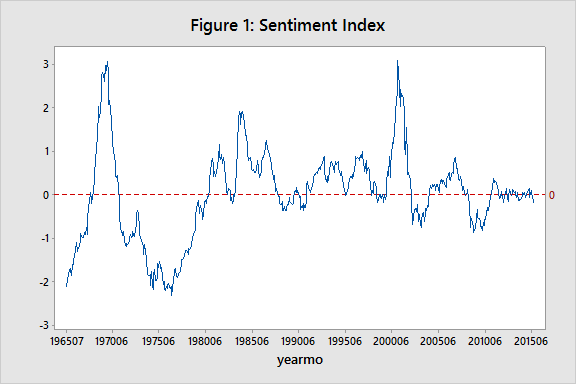
\includegraphics[width=\textwidth]{chapters/chapter_news_an/figures/ch4sec1sentimentindex.png}
	\caption{Sentiment Index.\label{fig:sentimentindex}}
	\end{figure}

While the extensive discussion of these results at the stock level is not possible here, we want to present the descriptive statistics of key performance indicators and other associated characteristics at the market level. The goal of this exercise is to show how conditional on the sentiment scores the averages over different key characteristics differ. The data on Fama-French factor model, see Fama and French (2015)~\cite{fama2015international}, is taken from French's website. It consists of (details are directly from the site):

\begin{itemize}
\item SMB (Small Minus Big) is the average return on the nine small stock portfolios minus the average return on the nine big stock portfolios.

\item HML (High Minus Low) is the average return on the two value portfolios minus the average return on the growth portfolios.

\item RMW (Robust Minus Weak) is the average return on the two robust operating profitability portfolios minus the average return on the two weak operating profitability portfolios.

\item CMA (Conservative Minus Aggressive) is the average return on the two conservative investment portfolios minus the average return on the two aggressive investment portfolios.

\item $R_m-R_f$, the excess return on the market, value-weight return of all CRSP firms incorporated in the US and listed on the NYSE, AMEX, or NASDAQ that have a CRSP share code of 10 or 11 at the beginning of $t$, and good return data for $t$ minus the one-month Treasury bill rate (from Ibbotson Associates).
\end{itemize}

The daily data on the above factors for the same duration as the duration of the sentiment data given in Figure~\ref{fig:varexcess} was collected and aggregated to match the monthly level sentiment data. For the excess return, $R_m-R_f$ we compute the monthly averages and as in Yu and Yuan (2011)~\cite{yuyuan}, we compute the realized variance of the excess return as,
	\begin{equation}\label{fig:varexcess}
	\widehat{\sigma}_t^2=\frac{22}{N_t}\sum_{t=1}^{N_t}(R_{mt}-R_{ft})^2
	\end{equation}
where $N_t$ is the number of trading days in a month. The aggregated factors are plotted in Figure~\ref{fig:timefamafrench}.
 
	\begin{figure}[!ht]
	\centering
	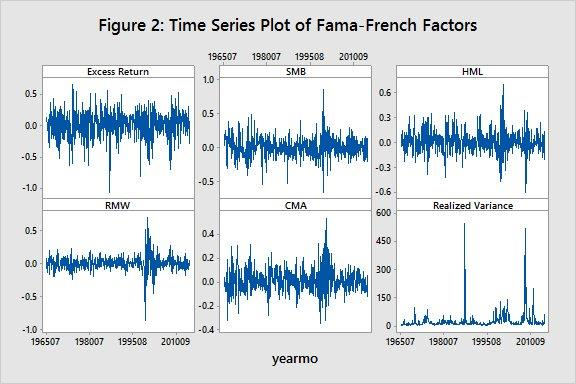
\includegraphics[width=\textwidth]{chapters/chapter_news_an/figures/ch4sec1famafrench.jpg}
	\caption{Time Series Plot of Fama-French Factors.\label{fig:timefamafrench}}
	\end{figure}

To classify the sentiment into low and high Baker and Wurgler (2006)~\cite{baker2006investor} simply use the negative and positive scores. In order to allow for the natural variation in the sentiment scores, we classify the score below the first quartile ($-0.5$) as low sentiment and the score above the third quartile ($+0.5$) as high sentiment and in between as normal sentiment. Table 4.1 provides the summary. The contrast between the low and high sentiment periods is quite evident.

\begin{table}[!ht]
\caption{Fama \& French Factors Across Sentiment Levels \label{tab:famafrench}}
	\begin{tabular}{lllll}
& Low &     Normal      & High & All \\ \hline

N & 152 &  283  & 168 & 603 \\

Sentiment & -1.297 &  0.031  & 1.120 & 0.000 \\

Excess Return & 0.0127 &  0.044  & -0.004 & 0.023 \\ 

SMB & 0.031 &  0.009  & -0.010 & 0.009 \\

HML & 0.014 & 0 & 0.052 & 0.018 \\

RMW & -0.001 &  0.007  & 0.035& 0.013 \\

CMA & 0.011 &  0.003  & 0.040 & 0.016 \\
 
Realized Variance & 23.89 &  24.58  & 16.83 & 22.25
	\end{tabular}
\end{table}

Some observations follow: While the pattern in excess return is consistent with what is observed in Yu and Yuan (2011)~\cite{yuyuan}, the realized variance in high sentiment period is lower than the other periods, but this is consistent with the mean-variance relationship as expected by the asset pricing models. The SMB which measures the difference in returns between small stocks and large stocks is negative during high sentiment periods indicating the portfolio of small stocks does not do well in these periods. The HML, the difference in returns between high and low B/M stocks tends to be positive and higher during high sentiment periods. The RMW which measures the performance difference between robust and weak profitability portfolios is also higher during high sentiment periods. Finally, CMA, which measures the difference in performance between conservative and aggressive firms continue to do well in high sentiment periods.


Da, Engleberg, and Gao (2011)~\cite{da2011search} review studies on investor attention and its impact on stock performance. The proxies such as extreme returns, trading volume, news and headlines, advertising expense etc. were used as indirect measures of attention. Because some of these proxies can be driven by factors unrelated to investor attention, it must be noted that they, at best, are proxies. Instead it is suggested that search frequency of key words related to a stock in a search engine is a more direct measure of the attention as the users who search directly express their intent and thus their interest.


Google publishes the search volume index (SVI) for the key words and except for rarely-searched tail terms, the index is fairly reliable due to the significant market share of Google in terms of search volume compared to other search engines. Da et al. (2011)~\cite{da2011search} find SVI is a leading indicator of extreme returns and news and the abnormal SVI matches with the known anomalies. Generally we must emphasize that what are meant by anomalies are any empirical deviations from what are postulated by economic theory. A positive abnormal SVI generally predicts higher stock prices in the short term and price reversals in the long term.


Da, Engleberg, and Gao (2015)~\cite{da2015sum} extend this idea to study the market-level sentiment and its correlation to aggregate market returns. The market-level index is based on the top thirty search terms that relate to general public's concern, such as unemployment, recession, bankruptcy, etc. The index is shown to predict short-term return reversals, increase in volatility and flows from equity funds to bond funds. The change in the index is demonstrated to be correlated with certain sentiment indicators, of Baker and Wurgler (2006)~\cite{baker2006investor}.


Stambaugh et al. (2012)~\cite{stamb} consider several asset-pricing anomalies that may be attributed to financial distress, momentum, asset growth etc. For each anomaly, the strategy that goes long in the highest-performing decile and goes short in the lowest-performing decile is examined. However as Huang et al. (2015)~\cite{huang} observe, ``\dots whether investor sentiment can predict the aggregate stock market at usual monthly frequency is still an open question.'' It must be noted that the market is efficient for the most part and impounding any information occurs rather immediately at the higher frequency level. Thus there is a great deal of interest to mine news, attention and sentiment as they occur and the information from social media has come to play an effective role. We present some evidence to that effect in the next section. 


\section{Market Micro Structure and Liquidity}
\section{Automated News Analysis and Market Sentiment}


Trading now mostly occurs at a relatively high frequency level and hence any news related to a stock gets processed almost instantaneously. The literature reviewed earlier refers to low frequency sentiment data and hence its influence on returns is not easy to notice. New technologies that can handle automatic news collection, extraction and categorization of relevant information are fast-emerging. Quantitative models that incorporate this information in investment decisions are being actively researched and automation of these activities can greatly help traders shortening their reaction time to emerging news feeds.


There has been a surge of academic interest in this topic (see Mitra and Mitra (2011)~\cite{mitra2} and Petersen (2016)~\cite{peterson}). Several technology companies (iSentium, MarketPsych, RavenPack, etc.) have sprung up in the last few years offering the service of aggregating the web information. Financial news can be classified into two main groups. Some financial news related to a stock are released on a regular basis, such as earnings statements and are well structured. The expectations on the earnings are formed based on the stock's other performance indicators and when the actual earnings differ from the trader's expectations, the trading decisions are normally adjusted for the a priori speculation. Then there are other news related to the product or personnel of the company that may come unscheduled and may affect the trading decisions. Although these are unstructured due to limited sources, they can be easily processed. Usually the early exploiters of the information can expect to gain some advantage over others. These are generally termed as news-based event strategies and have been fairly well-studied in the finance literature. 


Unstructured news streams come at irregular intervals and are usually textual and qualitative. In order to correlate this information with the stock performance, they need to be appropriately quantified and because this information originates from numerous sources such as in social media, it needs to be properly aggregated. Without any aggregation it may be difficult to extract the signal from the noise. Some common steps involved in making the news useable for trading are:
	\begin{enumerate}[--]
	\item Identify the unique and relevant news on a timely basis.
	\item Quantify the textual information into informative scores, whose variation would cover negative to positive sentiment/connotation.
	\item Aggregate the scores from different sources.
	\item Develop a baseline model adjusting for seasonality of the sentiment scores.
	\item Relate the abnormal deviation of the sentiment scores to abnormal stock price movements. 
	\end{enumerate}
As many of these concepts and related issues are discussed in the references cited in this chapter, we will be brief in our discussion. Das and Chen (2007)~\cite{daschen} show how it is possible to capture the net sentiment from positive and negative views on message boards using statistical language techniques. The emotive sentiment is elicited using different classification algorithms and the results are pooled via majority voting. Opinions are extracted from message board postings and they are classified into three types: bullish, bearish and neutral. The classification algorithms include parts of speech tagging and support vector machines. The algorithms are initially trained using humanly preclassified messages and are designed to learn and apply these rules out-of-sample. Relating the sentiment to the performance of stocks in the Morgan-Stanley High-Tech Index it is observed that there is no strong relationship to individual stock prices but there is a statistical relation to the aggregate index performance. There is also a strong relationship between message volume and volatility consistent with Antweiler and Frank (2004)~\cite{antweiler2004all}.  


We want to briefly provide some details on a few providers of web analytics; interested readers should consult these providers' websites for further details.
\begin{enumerate}[--]
\item Ravenpack (NewsScore): The key information on entities (company, organization, currency, commodities and place) from major news sources are gathered and processed for their relevance and are assigned event sentiment score. The scores are aggregated on a rolling window basis. In addition, the aggregate count as event volume, the event novelty score, event novelty elapsed time etc. are provided. For equity markets, composite sentiment score and the impact projections of the news are also available. The main news providers are Dow Jones Newswires, The Wall Street Journal (all editions) and Barron's. 

\item Thomson Reuters (News Analytics): Data fields include relevant score of the news item to the asset, number of sentiment words or tokens, sentiment classification, novelty of the content, feed volume etc. The sources are Reuters, PR Newswire etc. 

\item Thomson Reuters (MarketPsych Indices): News and social media information in real time are delivered as data series; there are categorized into three types of indicators: Emotional indicators, Macroeconomic metrics and Buzz metrics on the asset level. The data is updated on a minute basis. The social media data includes blogs, internet-forums and finance-specific tweets.

\item iSentium (iSense): Extracts sentiment signals using natural language processing architecture on Twitter data; the data feed includes retweets, if the author has a finance-related bio, number of followers etc. The impact is measured by the number of retweets for each author's tweets. 
\end{enumerate}


In the next section, we will summarize studies that use the information provided by these agencies for developing trading strategies. To provide the theoretical underpinning of the effect of investor sentiment, two assumptions are made (see Delong, Shleifer, Summens and Walman (1990)~\cite{ssw}): market consists of two types of traders, noise and rational and they both are risk averse. Tetlock (2007)~\cite{tetlock2007giving} defines sentiment as the level of noise traders' random beliefs to rational traders' updated beliefs; it is argued that media (collective) pessimism is a proxy for either the sentiment or risk aversion and that it is expected that high media pessimism will predict low returns at short horizons and at longer horizons, a reversion to fundamentals will occur. 


\section{News Analytics and its Applications to Trading}


We have reviewed studies that have clearly documented the influence of news on stock market behavior. In this section, we will outline first the key methodologies used in relating the data on the inflow of news to key characteristics of stock trading and the stock performance indicators. A simple framework that we will follow is from Gloss-Klussmann and Hautsch (2011)~\cite{klub} and is depicted in Figure~\ref{fig:intervals}:

	\begin{figure*}[!ht]
	\centering
	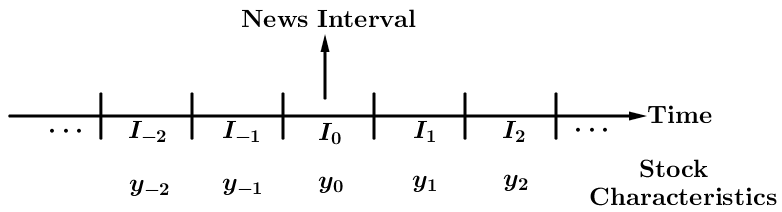
\includegraphics[width=4in]{chapters/chapter_news_an/figures/ch4sec4intervals.png} 
	\caption{News Interval.\label{fig:intervals}}
	\end{figure*}

The news arrival can generally be modeled as a point process but to remove any noisy friction in the data, both in the newsfront and in the stock price movement, it may be advisable to aggregate the information in short intervals. The stock characteristics can include the change in the price as well as volume, volatility, etc. during the interval. In addition to time aggregation, we also need to consider aggregation over different variables or dimensions of sentiment as in Baker and Wurgler (2006)~\cite{baker2006investor}. We describe these in two contexts below. \\


\noindent\textbf{Aggregation Over Dimensions:} \\


In the use of monthly data from Google, Da et al. (2015)~\cite{da2015sum} aggregate the daily change in a related search term, $i$, over the top thirty terms to come up with an index called, FEARS (financial and economic attitudes revealed by search) as 
	\begin{equation}\label{eqn:fears}
	\text{FEARS}_t = \sum_{i=1}^{30} R^i (\Delta \text{ASVI}_{it})
	\end{equation}
where $\Delta \text{ASVI}_{it}$ is an adjusted (winsorized, deseasonized, and standardized) daily change in search volume, 
	\begin{equation}
	\Delta \text{ASVI}_{it} = \ln(\text{SVI}_{it}) - \ln(\text{SVI}_{it-1})
	\end{equation}
Here $R(\cdot)$ denotes the ranking function. Generally search volume data exhibits non-stationarity as well as strong weekday seasonality. It has, for instance, been found that web searches tend to be higher on Monday through Wednesday than on other days. The above adjustments to search volume take care of both concerns. The Equation (\ref{eqn:fears}) is essentially a differencing operator that addresses the stationarity and a similar differencing for the weekday effect can be easily incorporated. These ideas were discussed in Chapter 2. 


The sentiment index in Baker and Wurgler (2006)~\cite{baker2006investor} is a composite index based on the five standardized sentiment proxies mentioned earlier. Because some variables take longer to express the same sentiment, the proxies are lagged. The series are smoothed over the prior twelve months and the index uses the $t-12$ value. The new series do not use turnover, due to fragmentation, NYSE is no longer the dominant venue. 


In the construction of this index, it appears the principal component of the five variables and their lags are used. Thus the first stage index has ten loadings; using the correlation between the index and current and lag values of the variables, the time index that is most appropriate for each of the variables is selected. In the original construction, the variables RIPO and PD-ND are lagged but the rest are used as of current time. The sentiment index is also further refined to adjust for a common business cycle components measured through growth in the industrial production index, growth in consumer durables, nondurables and services and an indicator variable for NBER recessions. The regression residuals are argued as better, cleaner measures of sentiment. These are then used in the principal component analysis. Thus mathematically, if $x_t=(x_{1t},x_{2t},\cdots,x_{5t})'$, the first principal component is obtained by
	\begin{equation}
	\max_l \; l' \textstyle \sum_{xx} l \quad\quad ; \, l'l=1 
	\end{equation}
Because the variables are standardized, it should be noted that the covariance matrix, $\sum_{xx}$ is also the correlation matrix. The first linear combination is associated with the eigenvector that corresponds to the largest eigenvalue of the matrix, $\sum_{xx}$, gives the sentiment score,
	\begin{equation}\label{st}
	s_t= \dfrac{l' x_t}{\sqrt{\lambda}}
	\end{equation}
in Figure~\ref{fig:intervals}. Here $\lambda$ is the largest eigenvalue of $\sum_{xx}$ so that the sentiment score, $s_t$ is taken to have unit variance. \\


\noindent\textbf{Relating Sentiment to Stock Performance:} \\


The general framework relating the sentiment scores ($s_t$) to performance indicators ($y_t$) is simply through lagged regression. For example, the returns $R_t(y_t)$ are related to ($s_t$) and other control variables and can take the form:
	\begin{equation}\label{rs}
	R_{t+k}= \beta_0 + \beta_1 s_t + \gamma' z_t + u_{t+k}
	\end{equation}
where $z_t$ is a set of control variables that may be related to the stock, such as Fama and French factors. The left side can also be (annualized) realized volatility, calculated by sampling the price over `$N$' times during a day. 
	\begin{equation}
	rv_t = 250 \sum_{d=1}^N r_{t,d}^2
	\end{equation}
Because of the persistence of the volatility, some adjustments via differencing should be considered when relating sentiment scores to volatility. Finally, it is possible that the effect of positive sentiment on stock returns could be different from that of negative sentiment. Fitting models similar to (\ref{rs}) for both scenarios separately would be a worthwhile exercise. \\


\noindent\textbf{Aligned Investor Sentiment:} \\


In the above set-up, the construction of the sentiment scores (Equation \ref{st}) or FEARS (Equation \ref{fears}) is done first and then it is related to--for instance--the returns via (\ref{rs}) subsequently. Huang, Jiang, Tu and Zhou (2015)~\cite{huang} combine the two steps, together arguing the linear combination in (\ref{st}) is constructed better in referencing to the stock characteristics and not on its own. They propose the partial least squares (PLS) method advanced by Wold (1984)~\cite{wold}. \\


\noindent \textbf{Partial Least Squares:} Partial least squares by Wold (1984)~\cite{wold} is an iterative computational algorithm for linear regression modeling, especially for situations where the number $n$ of predictor variables ($X_t$) is large. The $m \times 1$ multiple response, $X_t$ ($m>1$) version of partial least squares begins with a `canonical covariance' analysis, a sequential procedure to construct predictor variables as linear combinations of the original $n$-dimensional set of predictor variables $X_t$. At the first stage, the initial predictor variable $X_{1}^*=b_1'X_t$ is determined as the first `canonical covariance' variate of the $X_t$, the linear combination of $X_t$ that maximizes $\{(T - 1) \times \text{sample covariance of } b'X_t \text{ and } l'Y_t \} \equiv b' \mathbf{XY}' l$ over unit vectors $b$ (and over all associated unit vectors $l$). For given vectors $b$, we know that $l=\mathbf{YX'} b/(b' \mathbf{XY'YX'}b)^{1/2}$ is the maximizing choice of unit vector for $l$, so that we need then to maximize $b' \mathbf{XY'YX'}b$ with respect to unit vectors $b$. Thus, the first linear combination vector $b_1$ is the (normalized) eigenvector of $\mathbf{XY'YX'}$ corresponding to its largest eigenvalue. (In the univariate case, $m=1$ and $\mathbf{Y}$ is $1 \times T$, and so this reduces to $b_1=\mathbf{XY'}/(\mathbf{YX'XY'})^{1/2}$ with associated ``eigenvalue" equal to $\mathbf{YX'XY'}$.)


At any subsequent stage $j$ of the procedure, there are $j$ predictor variables $x_{it}^*= b_i' X_t, i=1,\cdots,j$, determined and the next predictor variable $x_{j+1}^*= b_{j+1}'X_t$; that is, the next unit vector $b_{j+1}$ needs to be found. It is chosen as the vector $b$ to maximize the sample covariance of $b'X_t$ and $l' Y_t$ (with unit vector $l$ also chosen to maximize the quantity); that is, we maximize $b' \mathbf{XY'YX'}b$, subject to $b_{j+1}$ being a unit vector and $x_{j+1,t}^*=b_{j+1}; X_t$ being orthogonal to the previous set of $j$ predictor variables $x_{it}^*, i=1,\cdots,j$ (i.e. $b_{j+1}' \mathbf{XX'} b_i=0$, for $i=1,\cdots,j$). The number $w$ of predictors chosen until the sequential process is stopped is a regularization parameter of the procedure ; its value is determined through cross-validation methods in terms of prediction mean square error. The final estimated regression equations are constructed by ordinary LS calculation of the response vectors $Y_k$ on the first $w$ `canonical covariance' component predictor variables, $X_k^*=(x_{1k}^*,\cdots,x_{wk}^*)' \equiv \hat{B} X_k$, where $\hat{B}=[b_1,\cdots,b_w]'$; that is, the estimated regression equations are $\hat{Y}_k= \hat{A}X_k^* \equiv \hat{A}\hat{B} X_k$ with
	\[
	\hat{A}=\mathbf{YX}^{*'} (\mathbf{X}^* \mathbf{X}^{*'})^{-1} \equiv \mathbf{YX'} \hat{B}' (\hat{B} \mathbf{XX'} \hat{B}')^{-1}
	\]
and $\mathbf{X}^*=\hat{B}\mathbf{X}$ is $w \times T$. In practice, the predictor variables $X_k$ and response variables $Y_k$ will typically already be expressed in terms of deviations from sample mean vectors.


Discussion of the sequential computational algorithms for the construction of the `canonical covariance' components $x_{jk}^*=b_j'X_k$ required in the partial least squares regression procedure, and of various formulations and interpretations of the partial least squares method are given by Wold (1984)~\cite{wold}, Helland (1988,1990)~\cite{helland88}~\cite{helland90}, and Garthwaite (1994)~\cite{garth}. In particular, for univariate partial least squares, Garthwaite (1994)~\cite{garth} gives the interpretation of the linear combinations of predictor variables, $x_{jk}^*=b_j'X_k$, as weighted averages of predictors, where each individual predictor holds the residual information in an explanatory variable that is not contained in earlier linear combination components ($x_{ik}^*, i<j$), and the quantity to be predicted is the $1 \times T$ vector of residuals obtained from regressing $y_k$ on the earlier components. Also, for the univariate case, Helland (1988,1990)~\cite{helland88}~\cite{helland90} showed that the linear combination vectors $\hat{B}=[b_1,\cdots,b_w]'$ are obtainable from nonsingular ($w \times w$) linear transformation of $[\mathbf{XY'}, (\mathbf{XX'})\mathbf{XY'},\cdots,(\mathbf{XX'})^{w-1} \mathbf{XY'}]'$. 


Huang et al. (2015)~\cite{huang} demonstrate that the new combination of predictors based on PLS method has much greater predictive power for the aggregate stock market and its predictability is both statistically and economically significant. \\


\noindent \textbf{Social Media/Twitter Data:} Over the past years, significant development has been made in sentiment tracking technologies that can extract indicators of public mood from social media such as blogs and Twitter feeds. Although each Tweet is of limited number of characters, the aggregate of Tweets may provide an accurate representation of public sentiment. This has led to the development of real--time sentiment tracking tools (Opinion Finder, GPOMS (Google Profile of Mood Status), etc.) to track the public mood and relating them to economic indicators. Crowd--sourced data generated by social network sites such as Twitter/StockTwits is being increasingly used by quantitative researchers to generate trading signals. The wisdom of the crowd surprisingly appears to outperform the wisdom of the experts in a variety of instances. For a recent application relating sentiment data to earnings announcement, see Liew, Guo and Zhang (2017)~\cite{liewzhang}. We now illustrate a simple trading algorithm using the iSentium data.


iSentium expertise lies in providing market sentiment indicators. Market--related texts from Twitter are processed through Natural Language Processing Techniques and the contents are assigned sentiment scores in the range of $-30$ to $30$ with positive score indicating optimistic view and the negative score, a pessimistic view. For a specific keyword the data contains the following information: \\

\begin{enumerate}[--]
\item Time when the Tweet is recorded
\item Sentiment Score
\item Total number of Tweets since Jan 1, 2012
\item Whether it is a retweet
\item Whether the author has a finance--related bio
\item Number of followers of the author
\item Number of Tweets posted by the author
\item Average number of retweets for each of the author's Tweets, measuring the author's impact. \\
\end{enumerate}


In addition to per--tweet data, the company also provides binned data, binned over various time durations. Surprisingly tweet volume is high for popular ETFs and large cap technology stocks. To illustrate, we consider the per-tweet data from Jan 1, 2012 to September 10, 2014 for the \textbf{ESMini} (ticker symbol: \textbf{QQQ}). The typical data is listed in Table~\ref{tab:isentiumdata}:

\begin{table}[!ht]
\centering
\caption{Typical Elements of iSentium Data \label{tab:isentiumdata}}
\hspace*{-1.8cm}
\begin{tabular}{rrrrrrrrrr}
Date & Time & SS & Retw & Retwld & authid & FinBio & nfollow & ntweets & impact \\
1/1/2012 & 3:04:41 & 9 & 0 & $-1.00\text{E}+00$ & 202647426 & 1 & 222 & 16 & 0 \\
1/1/2012 & 3:10:06 & 9 & 0 & $-1.00\text{E}+00$ & 23059499 & 1 & 10501 & 27 & 0 \\
1/1/2012 & 3:19:46 & $-11$ & 0 & $-1.00\text{E}+00$ & 202647426 & 1 & 222 & 25 & 0 \\
1/1/2012 & 3:43:52 & 0 & 0 & $-1.00\text{E}+00$ & 202647426 & 1 & 222 & 30 & 0 \\
1/1/2012 & 3:50:01 & 0 & 0 & $-1.00\text{E}+00$ & 23059499 & 1 & 10501 & 48 & 0 \\
1/1/2012 & 4:10:01 & $-5$ & 0 & $-1.00\text{E}+00$ & 23059499 & 1 & 10500 & 89 & 0 \\
1/1/2012 & 4:11:02 &  $-5$ & 0 & $-1.00\text{E}+00$ & 207429198 & 0 & 51 & 2 & 0 \\
1/1/2012 & 4:12:10 &  $-5$ & 1 & $1.53\text{E}+17$ & 16704290 & 1& 1170 & 3 & 0 \\
1/1/2012 & 4:26:07 & $-10$ & 0 & $-1.00\text{E}+00$ & 207429198 & 0 & 51 & 9 & 0 \\
1/1/2012 & 4:30:03 & $-10$ & 0 & $-1.00\text{E}+00$ & 23059499 &	1 & 10500	 & 104 & $0.0625$ 
\end{tabular}
\end{table}

It is quite apparent from the short list of entries in Table~\ref{tab:isentiumdata}, the same author of a tweet can have varying sentiments in a short duration of time. It is also likely that a few authors can dominate the number of tweets in a short duration ($\approx$90 minutes in the sample data in Table~\ref{tab:isentiumdata}). Consequently in the application we describe here, the daily summaries of sentiment scores are calculated and matched with the daily performance of ESMini. Note that twitter activity occurs every day but the markets are open only on weekdays. No attempt is made to account for the cumulative effect of weekend sentiment scores on the beginning-of-the-week ESMini performance. The ESMini data contains daily price bars (with open, high, low and close) and the volume of transactions.


The time series plot of the sentiment related variables and the ESMini trade related variables are given in Figure~\ref{fig:sentimentesmini}. Here the variables are defined as:
\begin{enumerate}[--]
\item RetO$=\ln(P_{t_0}) - \ln(P_{t-1.0})$ based on opening price
\item Volume is logged
\item Volatility$= 0.5(H_t-L_t)^2 - 0.386(C_t-O_t)^2$, where $H_t=\ln(P_{tH})$, the high price observed during the day etc.
\item SSAav is the average sentiment score for the day
\item FBav is the proportion of tweets by the tweeters with a finance bio
\item Retav is the average number of retweets per day 
\end{enumerate}
While one focus is on sentiment score, the other two sentiment variables indicate the intensity of activity by the twitter participants in the finance field. 

	\begin{figure}[!ht]
	\centering
	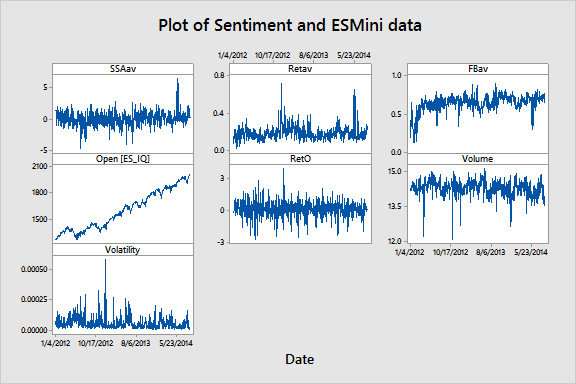
\includegraphics[width=\textwidth]{chapters/chapter_news_an/figures/ch4sec4sentimentesmini} 
	\caption{Sentiment score and ESMini. \label{fig:sentimentesmini}}
	\end{figure}

It can be seen from Figure~\ref{fig:sentimentesmini}, that the sentiment average (SSAav) exhibits some variation over time but it is generally stationary. There is some memory in the series as the first few autocorrelations are found to be significant. All the other sentiment related series also exhibit some memory. The same can be noted for the volume and volatility series as well. One of the key tools to connect two series in terms of lead-lag relationships is the cross-correlation function defined in Chapter 2. For the sentiment data ($s_t$) to be of any predictive use, it should be correlated to lead return ($r_{t+k}$) and lead volatility ($V_{t+k}$). Figures~\ref{fig:ccfssavreto} and \ref{fig:ccfssavvol} capture the cross-correlation, but one can observe that there is some concurrent correlation between $s_t$ and $V_t$. This may be due to the fact that the aggregation of data was done over the entire day, which may be too long a duration for aggregation. These relationships can be confirmed in Table~\ref{tab:regesmini} with stepwise regression model fit. 

	\begin{figure}[!ht]
	\centering
	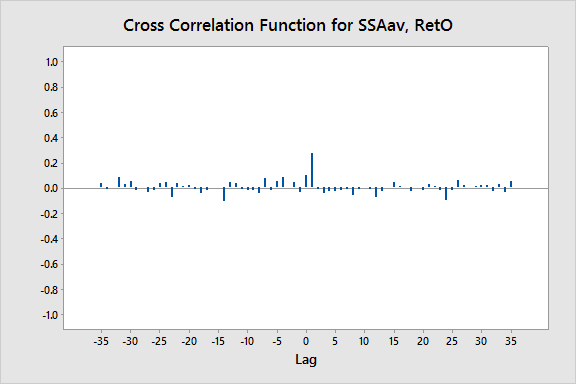
\includegraphics[width=\textwidth]{chapters/chapter_news_an/figures/ch4sec4crossfssaavreto} 
	\caption{CCF(SSAve $\rightarrow$ Reto). \label{fig:ccfssavreto}}
	\end{figure}

	\begin{figure}[!ht]
	\centering
	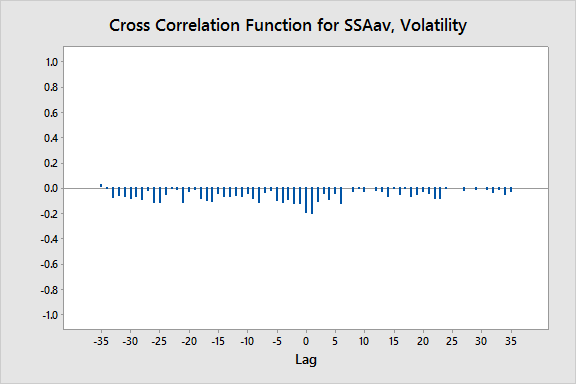
\includegraphics[width=\textwidth]{chapters/chapter_news_an/figures/ch4sec4ssaavvola} 
	\caption{CCF(SSAve $-$ Reto). \label{fig:ccfssavvol}}
	\end{figure}

	\begin{table}[!ht]
	\centering
	\caption{Regression of ESMini variables on sentiment factors \label{tab:regesmini}}
	\begin{tabular}{rrrr}
	\multicolumn{4}{c}{Response Variable} \\
	Predictors & Return & Volume & Volatility \\ \hline
	SSAav & --- & $-0.0482$ & $-0.00005$ \\
	SSAverlag & $0.1895$ & $-0.0291$ & $-0.00006$ \\
	AuHTAV & --- & $-0.000017$ & $-0.000001$ \\
	RetAV & --- & --- & $-0.000063$ \\
	NfollowAV & --- & --- & $-0.000001$ \\
	AVetW & --- & --- & $0.000047$ \\
	Constant & $0.0759$ & $14.41$ & $0.000085$ \\ \hline
	$R^2$ & $0.0732$ & $0.1154$ & $0.1357$ \\ \hline
	\multicolumn{4}{c}{$\ast$All indicated factors are significant at 0.05 level}
	\end{tabular} 
	\end{table}

We propose two na\"ive strategies that can be used for trading using the sentiment data are proposed; both are in the spirit of the discussion related to sentiment data by Baker and Wurgler (2006)~\cite{baker2006investor}. The first strategy develops rules based on the sentiment scores and the second is based on the more direct regression relationship between returns and the sentiment scores: \begin{enumerate}[1.]
\item Crossover Strategy: If the difference between 3-day EWMA and 30-day EWMA of sentiment scores is positive, go long; otherwise go short. 
\item Open-to-open Strategy: Regress open-to-open returns on 10-day EWMA and its lag to predict the return; if positive, go long. Hold the position until the next day open. 
\end{enumerate}


It is easy to note that the moving average crossover strategy discussed in Chapter 3 is comparing the short term trend with the long term trend. The strategy exploits the deviation between the two. Both strategies can be evaluated on a moving window basis. Here we present results for the cross-over strategy only. As noted from Figure~\ref{fig:sentimentesmini}, the ESMini price has been steadily going up and thus a simple buy and hold strategy over time would be profitable. So we compare performance of the strategy with the buy and hold. The simple averages over buy and sell signals are quite revealing as seen from Table~\ref{tab:descstatcross}

\begin{table}[!ht]
\centering
\caption{Descriptive Statistics (Averages): Cross-over strategy \label{tab:descstatcross}}
\begin{tabular}{rrrrrrrr}
 & SSAve & RetAve & FBAC & Reto & Volume & Volatility & $N$ \\
Short  & $-0.5223$ & $0.1783$ & $0.6539$ & $-0.0866$ & $14.327$ & $0.000061$ & 333 \\
 Long & $0.4398$ & $0.1793$ & $0.6477$ & $0.2206$ & $14.220$ & $0.00044$ & 309 \\
 All & $-0.0592$ & $0.1788$ & $0.6509$ & $0.06125$ & $14.28$ & $0.000053$ & 642
\end{tabular} 
\end{table}

The negative signal from sentiment score matches with the negative return and higher volatility. The equity curve in Figure~\ref{fig:equitycross} clearly demonstrates the value of the strategy. 


\begin{figure}[!ht]
\centering
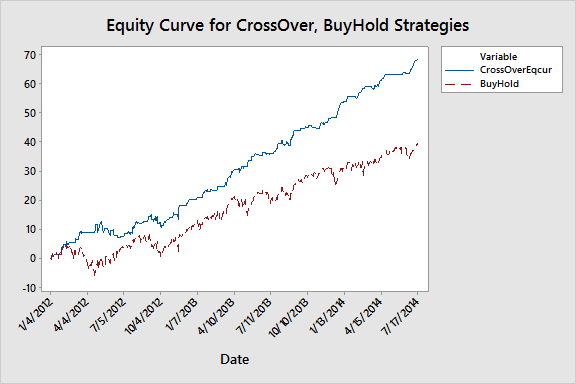
\includegraphics[width=\textwidth]{chapters/chapter_news_an/figures/ch4sec4equitycross} 
\caption{Equity Curve for ESMini. \label{fig:equitycross}}
\end{figure}


\noindent \textbf{Bloomberg News and Social Sentiment Data:} The news agency applies statistical machine-learning techniques to process the textual information related to equities and quantifies the sentiment both at the story-level and at the equity-level. The scores indicate at the story-level if the sentiment is positive, negative, or neutral with a confidence level; these are aggregated to provide the company-level sentiment. The computation is based on both news and Twitter feeds with a rolling window of half-an-hour. The predictive strength is tested out using the performance of the equity at a daily level as well as through changes in the stock price during the day. The approach is similar to cross-sectional momentum strategy that is outlined in Chapter 3. It can be shown that the stocks in the top decile of the day's sentiment scores tend to do better during that day. 


The sentiment data also can be used to predict the nature of earnings report. The event driven strategies are still a significant part of trading strategies and it can be shown that sentiment scores prior to earnings releases can augment these strategies. The intraday strategy is based on using the arrival of information during an interval of pre-defined duration and making trading decisions based on the sentiment scores and their confidence. Generally traditional news combining with a twitter feed can generate stronger signals. A methodology used to relate sentiment scores whether from traditional news or from twitter is to first construct an index, 
	\begin{equation}\label{eqn:itwithln}
	I_t= \ln\left( \dfrac{1+\|B_{u_t}\|}{1+\| B_{e_t}\|}\right)
	\end{equation}  
that adjusts for the baseline activities, here $B_{u_t}$ denotes the number of bullish tweets and $B_{e_t}$ denotes the number of bearish tweets. Defining the intraday return, $R_t=\ln(s_t^{\text{close}}) - \ln(s_t^{\text{open}})$, where $s_t$ refers to the stock price on a given time unit. Then forming, $y_t=(I_t^N,I_t^{TW},R_t)'$, VAR model that was discussed in Chapter 2 is used to identify the lead-lag relationships; here $I_t^N$ is the index for the news sentiment, such as Google search volume for relevant keywords and $I_t^{TW}$ refers to the index based on Twitter data. The VAR model provides a neat framework to consider other information such as market volume, market volatility, etc. that can be easily incorporated. 


Thomson Reuters MarkerPsych Indicies (TRMI): The TRMI are also based on news and social media that produce three key types of indicators: Emotional indicators, Macroeconomic metrics and the so called Buzz metrics. These are updated on a minute basis and covers various economic entities. The indices cover over fifty items and they are scored from $-1$ to 1 or from zero to 1. 


\section{Discussion / Future of Social Media News}



\part{Execution Algorithms}
% !TEX root = ../../../book.tex

In this part of the book we cover the other core topic of this book: Execution Strategies. Once again we will strive to give the reader the practitioner perspective and context, the necessary building blocks to fully grasp the subject and finally the quantitative underpinning where available.  Our hope is that by the end of the chapter our readers would have enough understanding of the topic to be able to, if asked, to implement at least a basic implementation of an execution product and be able to create the supporting Pre and Post-trade analytics.


We start in Chapter~\ref{chap:ch_trade_data_models} by discussing the modeling of trade data. We focus on several fundamental topics that are critical to practitioners but often disregarded by other treatment of the subject. We provide details on many of the analytics used in practice. Chapter~\ref{chap:ch_mi_models} then goes into one of the fundamental subject of execution: Market Impact. We strive to bring in the intuition on the inner works of market impact and build the functional form of standard MI models from first principles. We then go into more details through a review of the sizable literature to guide the student that is interested in more depth. Finally, Chapter~\ref{chap:ch_exec_models} goes into the real meat of the topic by covering Execution strategies and its component. Here we strive to give a modern perspective that tries to address many of the misconceptions present in the industry with the hope of setting the reader in more solid footing from the start.


Let us get started!
% !TEX root = ../../book.tex

\chapter{Modeling Trade Data}

\section{Normalizing Analytics}
One of the challenging aspects of execution unlike other algorithmic trading subject is the large number of different types of stocks such strategies have to apply to. The same strategy will need to work for super liquid instruments that trade like water at the minimum tick size, and illiquid stocks that trade only very infrequently at wide spreads; Stock that have very stable and large sizes at the inside markets, and stocks whose nbbo changes many times every second. To complicate matters further the market micro-structure of each stock is not constant throughout the day or even between one day and the next in often predictable manner and execution strategies are expected to adapt to those changes. For example, immediately after the open there is a lot of trading activity as investor incorporate the effect of overnight news. The increased uncertainty on the stock valuation is reflected by a much higher volatility and spread. Once the period of so called Price Discovery is over (usually within 15-30m in US markets), the trading behavior settles in and activity is reduced and so do spreads and volatility. Activity the resumes towards the end of the day in particular due to the  fact that many funds are marked to the day's closing price. An example of inter-day variabilty is the impact due to Special Days such as futures, and options expiration, earning announcements, etc. In such occasion the activity patterns of the stocks are systematically different (e.g. the trading activity during futures/options expiration is heavily tilted towards the close since the settlement prices are related to the closing price on that day).

One could (and in some cases actually should) apply different strategies to achieve the same benchmark for different types of stocks and different days or time of day but that is never done as it would be completely unwieldy and prohibitively expensive to build and maintain. What is one to do?

The common practitioner's approach is to parametrize many of the trading decisions using normalizing features, variables that help adapt the decision to a particular situation. This section will provide a review of the most common analytics and give pointers with regards to modeling approaches for each.  

The subject is quite extensive and would likely fill a medium-sized book on it's own. Additionally this subject, while extremely important in practice has gotten very limited treatment in academic research.

Thus ,while probably not scientifically satisfying, in this section we are forces to provide only a relatively coarse treatment of the subject from a practitioner perspective. It should however be sufficient as a starting point for anybody attempting to build basic Execution Algorithms and a foundation for deepening the subject.

\subsection{Basic Analytics}
\subsubsection{Order Size  Normalization: The Daily Volume}
A trader needs to execute an order for 1M shares of XYZ. Is this a big order she will have to carefully manage or a tiny order she can simply "fire and forget".  Intuitively due to large difference in stock characteristics and liquidity order size must be clearly viewed as a relative measure. The most commonly used by practitioners is the Average Daily Volume (ADV). Even a simple measure like this is cause of a lot of confusion lack of standard approaches and while the term ADV has a specific mathematical meaning it should be considered as a generic term for metrics that forecast the expected next day volume of a stock. 

As a baseline metric that 64 days Mean or Median daily volume are probably the most commonly used metric in the investment community. The 64 days horizon reflects length of a quarterly earning cycle and thus it's viewed as incorporating  all the seasonal effects of the daily volume.
 
%TBD Might want to have a graph of an 64d volume for a stable stock to show the spikes in various predictable places (earnings day, special days, etc)?%

%TODO Academic research on Daily Volume

\subsubsection{Time-scale Normalization }
Trading dynamics have an intrinsic timescale that varies significantly across the stock universe and it is often important to take this into consideration. For instance many of the normalizing analytics we'll discuss in the next section are based on intraday averages. The sampling bin size used should not be the same for each stock or one would have spurious statistical effects but rather it should sample at a rate that is consistent with how frequently things change.  As a trivial example measuring the average number of trades every 1s for a very illiquid stock that trades 10 times in a day would clearly have little practical value. 

Evaluating the state of an order during execution should also take the intrisic timescale (often called Characteristic Time) into consideration. For example on would not post a slice of the order passively and re-evaluate his decision after 1s if in average the queue in front for the order takes 3 minutes to clear.

Practitioner have found that a good normalization variable for such timescale is to look at the median time it takes for the quote to move. This metric is often called Turnover Time. 

Turnover time can be defined as:
%TODO what is the right way to mathematically represent turnover time?

While clearly more sophisticated approaches can and have been the important thing is to use it in a consistent fashion across  the various concerns. That usually leads to a much more stable behavior and improved decision making.

\subsubsection{Return Normalization: Quote Volatility}
%TODO


\subsubsection{Microstructure Normalization}
%% One critical concern one has to take in trading, in particular when trading very large sizes,  is the minimization of information leakage. Any unusual trading pattern that can be measured in the market data that could reveal to other participant that there is a large buyer or seller in the market could have dramatic deleterious effects on the the stock price. As such it is important to mask the intention by using "standard" behavior. This is another common use of normalizing variables. %%

The following is a brief overview of these decision and what analtyics are commonly used.
%TODO

\subsection{Intraday Normalization: Profiles}
Incorporating intraday seasonality it's a critical component of competent decision making in execution strategies. Intraday seasonality arise from primarily behavioral and practical reasons around trading discontinutities such as the open and the close (and the lunch break period in certain asian markets) and other scheduled events ( e.g. the US open for European markets). Information dissemination tends to cluster around such times and so then does trading activity. This is compounded by various conventions on how to value certain instruments and other benchmarks. In this section with ignore the fact that certain markets have lunch breaks. This clearly complicates but does not change the overall picture or approach and it's a relatively trivial extension to the treatment of profiles. 
  
The standard practice to incorporate that is to normalize decisions via intrarday profiles, essentially functions (usually discrete) that provides the value either absolute but more often relative (either as a multiplier or as a percentage) of some daily measure. While most microstructure variables showcase some of this seasonality the most used profiles are:
\begin{itemize}
\item Volume Distribution: The percentage of the expected daily volume that will trade in a particular bin.
\item Volatility Distribution: The percentage of the expected daily volatility that will trade in a particular bin.
\item Spread Multiplier: The percentage deviation from the average spread in a particular bin
\end{itemize}

Of particular importance is the Volume Distribution (or profile) as this is the single most important variable used to create a VWAP strategy. For such a strategy, well see, that the volume profile is directly used as the execution schedule for the strategy. This will ensure that the strategy trades a proportionally larger slice of the order at times when more  volume is expected to trade and thus reduce the risk of trading at prices away from the period VWAP.

Volume is most invariably shaped like a flattened U. Volatility and spread both are shaped vaguely exponentially. Volume is clustered around the opening auction(s) and the first several minutes after the open. This makes intuitive sense as the market is re-opening after a trading halt and all new information accrued during the break needs to be incorporated. Spread and Volatility are also large over this period signifying the increased uncertainty around the stock valuation. After this period of heightened activity trading settles in and volume flattens out only to pick up again in the period before the closing auction as investment firms that  


\paragraph{Building Intraday Profiles}
Building stable profiles presents non trivial challenges at multiple levels both quantitative, logistical and data related. It will often boil down to matter of trade-offs, data availability, and cost to build and maintain. We provide some hopefully valuable pointers that should allow the reader to navigate around the hurdles and avoid common pitfalls

\subparagraph{Number of Profile Bins}
The decision of the # of profile bins is a trade-off between required precision and granularity during the most active periods of the day and the lack of stability due to lack of data/change in each bin. 1 minute bin is the most common choice in the industry.

\subparagraph{Per Stock Profiles vs. Clustered Profiles}
One of the first decisions to be made is whether to create individual profiles for each stock in the universe or use some sort of clustering/grouping. With a universe of several thousand different trading instrument it might be impractical to build and maintain stable individual profiles. Additionally the stability of the profiles is important in order for their use to be effective. Overly illiquid and slowly moving stock will usually make for poor single stock profiles.
A practical and common approach is too use a statistical clustering approach using the L2 norm as distance measure and using a grid search to identify the number of clusters that provides good separation using for example the elbow method (TBD add reference)

\subparagraph{Fitting Approaches}
There are many modeling approaches that are used in practice but there is limited systematic research in this space. 
%TODO Add pointers to exeisting research

While this would clearly fit within the supervised learning family of method more often than not no actual fitting takes place but some form of per-bin averaging over a certain length of history after which some form of smoothing is applied.

Care must be take to remove from the data-set days with predictable differences in profile shape. These "special days" should be modeled separately and we'll provide some pointers in a later paragraph. If one uses some form of regression model the special day could be incorporated as a dummy variable.

\subparagraph{Length of History}
Another common open question is the length of history that should be used. The more data is used the more stable to profiles are however unless great care is given to various seasonal effects and continues changes in market microstructure there is the risk for the profile no to incorporate more recent shifts. This is a particular concern in recent times as the explosion of ETF trading has been consistently shifting more and more volume towards the close. The length of history can be used as a hyperparameter to be trained on a per cluster basis.

\subparagraph{Volume Profile Smoothing}
intrady volume profiles tend to be extremely noisy and require smoothing to be effective. It was estimated (reference?) that without smoothing the volume profile perform worse than considering completely flat profiles. However care mus be taken to avoid smoothing over real behavioral discontinuities (e.g there is a predictable spike in volume in European profiles coincident with the US opening). These spikes usually are preceded by a period of reduce trading activity due to traders waiting for the predictable event. So care has to be take not to smooth these spikes to avoid spread this over previous bins that could cause the algorithm to overtrade during the period of reduced trading. On common approach is to remove statistically significant spikes and replace them with a local average for the purpose of smoothing and the re-applying the spike afterward. It has been shown that this approach improves the overall predictability of the profile

\subparagraph{Special Days}
Special days, as previously discussed, present additional challenges due to the limited number of datapoints available (e.g triple witching occurs only 4 time a year). So using larger clusters (one cluster as a limit) is often the only option. In order to maintain some of the  cluster characteristics a common approach is to use a "difference" profile.

\subsection{Advanced Analytics}
\subsubsection{Remainder of the Day Volume}
\subsubsection{Dynamic Profiles}
\subsection{Hidden Markov Models (HMM) for dynamic market microstructure:  Estimation of Parameter and States}
\subsection{Adaptive Particle Filters}

\section{Microstructure Signals}
\subsection{Imbalances}
\subsubsection{Quote Imbalances}
\subsubsection{Trade Imbalances}
\subsubsection{Passive Fill Probability}

\section{Models for LOB dynamics}


Before we formally present the models, we want to provide a review of how the analysis of LOB data has been approached. Biais, Hillion and Spatt (1995)~\cite{spalt} study the trading activity in Paris Bouse (a fully automated limit order market), the dynamics of order flow and how the order flow varies with the state of the order book and marketplace events relevant to the asset. It is found that the conditional probability of a limit order placement is larger when the bid-ask spread is larger and when the order book is not deep. If a market order has been placed the chance that the next order posted provides liquidity is generally higher. The placement of orders also follows a pattern with new orders coming in the morning when the price discovery occurs and cancellations and large orders occur in the evenings. The durations between trades do indicate that the intensity of trade varies during the course of a day. The main tool used in these calculations is contingency table which provides both marginal and conditional probabilities. \\

\noindent \textbf{Slope of LOB:} To begin with we can consider the slope of the order book both on the demand side and on the supply side using the quotes on both sides various depths (see Figure~\ref{fig:limitstocks}). This provides information on order book imbalance that can be helpful for the trader to decide on the optimal time to enter or to exist the market (see Figure~\ref{fig:limitstocks}). It is observed from Figure~\ref{fig:limitstocks} that the bid-ask spread is at least twice the difference between quotes at successive depths. Thus the slope of the book is steeper closer to the best quotes. \\
	\begin{figure}[!ht]
	   \centering
	   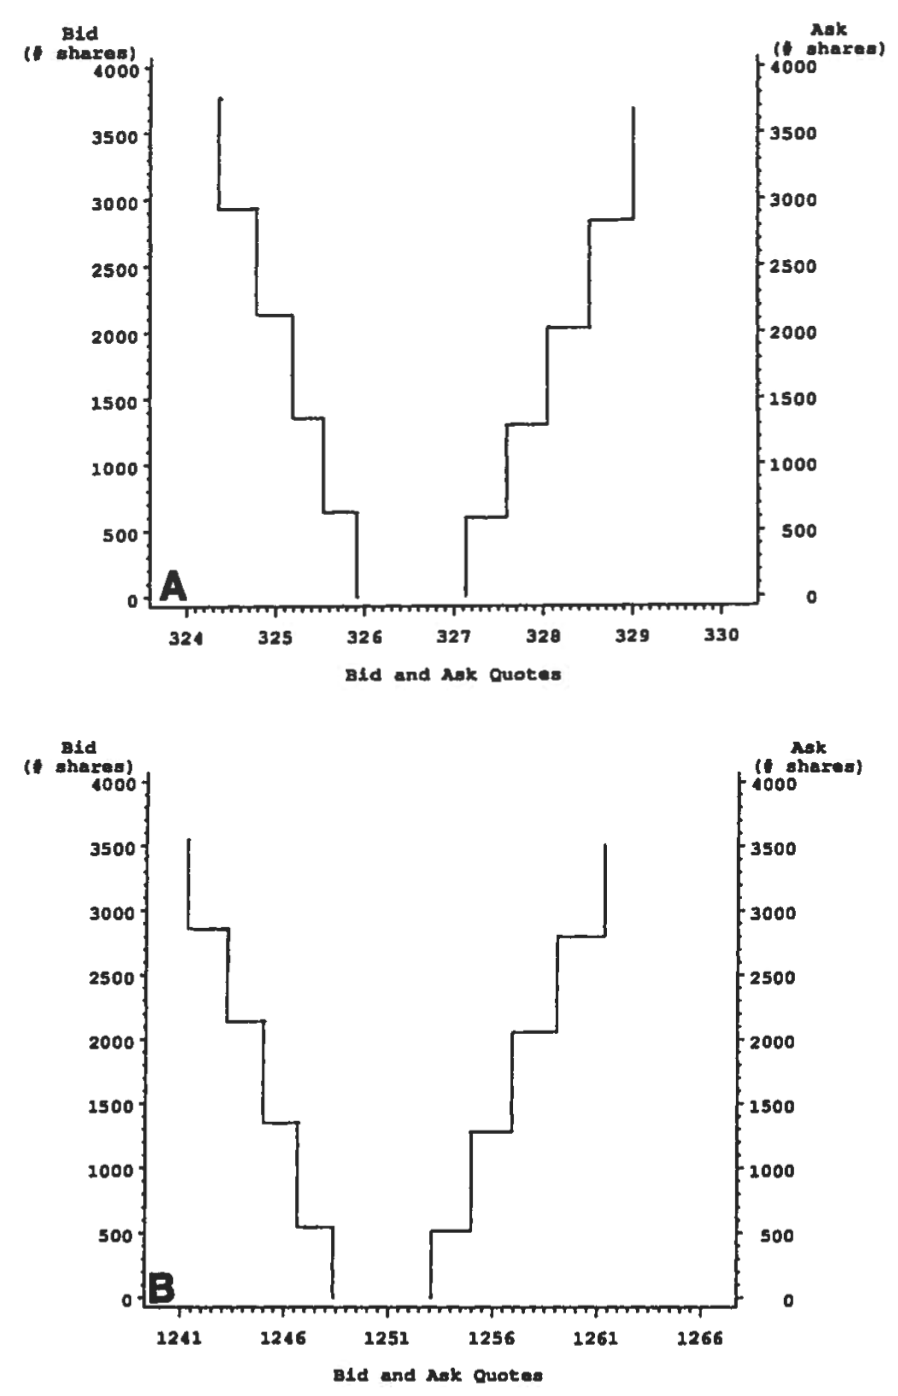
\includegraphics[width=0.75\textwidth]{chapters/chapter_trade_data_models/figures/limitstocks.png} 
	\caption{The Limit Order Book for Stocks. (A) Plots the cross-sectional average (across with tick$=$FF 0.1) of the time-series averages of the five best ask and bid quotes and their associated depth. (B) plots the cross-sectional average (across stocks with tick$=$FF 1) of the time-series averages of the five best ask and bid quotes and their associated depth.\label{fig:limitstocks}}
	\end{figure}

\noindent\textbf{Order Flow:} The orders can be characterized as buyer or seller initiated and how aggressive they are. The aggressiveness is quantified by the size of the order. Most of the orders are small indicating that they could be part of a large parent orders. Both placement and cancellation of orders seem to decrease away from the best quotes. As the intra-day trading pattern follows typical diurnal pattern, both the depth and order flow must be adjusted for the time of the day. Some observations (stylized facts) worth noting are:
\begin{enumerate}[--]
\item Large (small) trades on one side of the market tend to be followed by large (small) trades on the same side. The same thing could be said about the new limit orders and cancellations as well. It is speculated that this may be due to traders reacting similarly to the same events or due to parent order splitting and automatic placement of child orders. \\

\item Cancellations on the buy side of the book are more frequent after market buy orders and the same for sell orders. This may be due to the fact that the large sell orders tend to convey negative information about the stock while the large buy orders convey positive information. Cancelations may also occur because of placement of some market orders are intended to probe the presence of any hidden orders. \\

\item Conditioning on the state of the book by size of bid-ask spread and the depth, it is observed that trades are more frequent when the spread is tight but the new orders inside the quotes are more frequent when the spread is large. The changes in spread are mainly due to liquidity shocks. \\

\item Frequency of trades tends to be clustered because competing traders who monitor the market closely are likely to place the orders when they read the market in their favor. It is observed that the trading activity is more intense with the information flow. Also observed are the following stylized facts: when the spread is large after liquidity shocks, traders place their orders quickly to take advantage of time priority. Thus the spread reveals back to original level. The expected time interval is generally lower after large trades than after other trades whether the spread is large or not.
\end{enumerate}


Thus the study by Biasis et al. (1995)~\cite{spalt} provides a set of concrete measures that could be used to study the dynamics of the limit order book. Now we will delve into model formulations. 


One of the earlier models to appear in the econometric literature is by Lo, MacKinlay and Zhang (2002)~\cite{maczhang}; they used the data from Investment Technology Group (ITG) that contained time stamped information on each limit order from submission to cancellation or execution. With three possible paths for each submitted order, the associated (a) time-to-cancellation/modification, (b) time-to-first fill and (c) time-to-completion are tracked and models are developed for each path on both sides of the order. Because ITG largely deals with the institutional investors, the results apply only to a limited segment of the traders. The modeling approach is to get the execution times as the first-passage time to the limit price assuming that price follows a geometric Brownian model with a drift (Model 1.1):  
	\begin{equation}\label{eqn:dp(t)}
	dP(t)= \alpha \cdot P(t) \; dt + \sigma \cdot P(t) \; dW(t)
	\end{equation}
where $W(t)$ is a standard Brownian motion. A buy limit order with a price `$P_l$' is executed in the time interval $[t_0,t_0+t]$ only if $P_{\text{min}} \leq P_l$ and the probability is
	\begin{equation}\label{eqn:expprob}
	P_r(P_{\text{min}} \leq P_l \;|\; P(t_0)=P_0)= 1- \left(1 - \left(\dfrac{P_l}{P_0}\right)^{2\mu/\sigma^2}\right) \Phi\left[\dfrac{\ln(P_0/P_l) + \mu t}{\sigma \sqrt{t}}\right]
	\end{equation}
where $\mu=\alpha - \frac{1}{2} \sigma^2$ and $\Phi(\cdot)$ is the cumulative distribution function of the standard normal. 

Note (\ref{eqn:expprob}) can be alternatively stated as, if `$T$' denotes the limit order execution time, $F(t)=P(T \leq t \;|\; P_0)$ for buy orders and similarly for sell orders, $F(t)=p_r(P_{\text{max}} \geq P_l)$. To see if the model is appropriate for the data at hand compare the theoretical c.d.f. of $F(t)$ to empirical c.d.f. using the well-known result that these are uniformly distributed. Fix `$\tau$' as the fixed sampling interval and with $r_t=\ln(P_t)-\ln(P_{t-1})$, the estimates of $\mu$ and $\sigma^2$ are:
	\begin{equation}\label{eqn:sampleestm}
	\hat{\mu}= \dfrac{1}{N\tau} \sum_{j=1}^N r_j, \quad \hat{\sigma}^2= \dfrac{1}{N} \sum_{j=1}^N \dfrac{(r_j - \hat{\mu} \tau)^2}{\tau}
	\end{equation}
where `$N$' is the number of observations in the sample. 


The above First Passage Time (FPT) model was used for filled orders without taking into account that other orders that were cancelled or modified in that duration. The model's other limitations include not accounting for time priority, not including other relevant variables such as price volatility, spreads, etc.. The model's performance using the empirical cumulative distribution function is shown to be lacking. The model (\ref{eqn:expprob}) is expanded as
	\begin{equation}\label{eqn:cumexpmodel}
	F(t)=p_r(T_k \leq t \;|\; X_k,P_{lk}, S_k, I_k)
	\end{equation}
where $T_k$ is the execution of time of $k$ orders, $P_{lk}$ is the limit order price, $S_k$ is the size and $I_k$ is the side indicator. An alternative function, the hazard rate (briefly discussed in Chapter 2)
	\begin{equation}\label{eqn:hazard}
	h(t)=\dfrac{f(t)}{1-f(t)}= \dfrac{f(t)}{S(t)}
	\end{equation}
is found to be useful to operationalize and explain the modeling of survival rate of time-based events; Note $S(t)$ is called the survivor function. The censoring information ($\delta_i=1$ if observation `$i$' is censored) can be incorporated with $t_i$, $i$th realization of the random variable, $T$. It is assumed that the censoring mechanism is independent of the likelihood the limit order is executed. Using the generalized Gamma (defined in Chapter 2) as $f(t)$, the models are estimated.


The following variables are used as explaining variables:
\begin{enumerate}[--]
\item Distance between mid-quote and limit price.
\item Prior trade indicator for buyer or seller initiated.
\item Measures of liquidity.
\item Measures of market depth.
\item Measures that reflect change in trading activities. 
\end{enumerate}
It is shown that this model does fare better than FPT model to capture the execution times. But an important limitation is ``\dots censoring as a result of prices moving away from the limit price would be a violation of the underlying assumption since prices at the time of censoring are not included in $X_i$.'' We show in our analysis of Level III data, a key determinant for cancellation of an order is that price moving away from the limit price that the trader has desired. 


There are a number of studies that have looked into order book dynamics using models that arise from Point Processes. Bouchard, Mezard and Polters (2002)~\cite{bouchardmezard} investigate the interaction between order flow and liquidity; it is observed that the distribution of incoming limit order prices follow a power law around the current price and the overall shape of the book in terms of volume on both sides is rather systematic. Smith, Farmer, Gillemot and Krishnamunthy (2003)~\cite{smithfarm} and Farmer et al. (2004)~\cite{} study how the order flow influences price formation; the price impact of market orders is a function of touch price depth and spread size. Hewlett (2006)~\cite{} focuses on using LOB dynamics to find optimal liquidation strategies in foreign currency markets. 


To have a more complete and realistic picture of how the LOB evolves, we must consider `hidden liquidity'. Almost all exchanges allow traders to hide all or portions of their orders. The so called, ``iceberg order'' is split into several smaller parts and is queued along with the other orders, but only the displayed quantity is visible and is part of the market depth. When the order reaches the front of the queue only the displayed is executed. Several reports could be as high as 26\%. In the models discussed below, we will not address the hidden liquidity issue, which will be taken up in a later section.


Modeling of LOB dynamics has drawn on ideas from economics, physics, statistics and psychology. The approach taken in economics literature is to focus on the behavior of the traders and the dynamics is modeled as sequential games (Foucault (1999)~\cite{}, Parloys (1998)~\cite{} and Rosu (2009)~\cite{}). Others, such as researchers from physics, have treated order flows as random and statistical mechanics techniques are used to study the dynamics. Other studies, such as Parlour and Seppi (2008)~\cite{parseppi} and Bouchaud et al. (2009) are useful references for studies that come from economics point of view. We will review three models that are of recent origin. \\


\noindent\textbf{Cont, Stoikov and Talreja (2010)~\cite{contstoi}}: In this model of the limit order book, the number of limit orders at each price level in the book is taken to be a continuous-time Markov chain. The evolution of the order book through market orders, limit orders and cancellations is represented as a counting process. The model replicates the evolution of the events using independent Poisson processes. The study views LOB as a system of queues subject to order book events whose occurrences are modeled as a multidimensional point process. Before we state the specific questions and the models implications, we define certain useful quantities. 


It is taken that the price grid as $P(n)=\{1,2,\ldots,n\}$ multiples of a price tick. The number of outstanding orders in the book $|X_t^i|$ at price $i$, collectively, $X_t \equiv (X_t^1,\ldots,X_t^n)$ is taken to be continuous-time Markov chain; if $X_t^i<0$, then there are $-X_t^i$ bid orders at price `$i$' and if $X_t^i>0$, then there are $X_t^i$ ask orders at price $i$. Now we have,
	\begin{equation}\label{eqn:bestmidspread}
	\begin{split}
	\text{Best Ask Price: }& p_A(t)=\inf\{i \colon X_t^i>0\} \\
	\text{Best Bid Price: }& p_B(t)=\sup\{i \colon X_t^i<0\} \\
	\text{Mid Price: }& p_M(t)=(p_A(t)+p_B(t))/2 \\
	\text{Spread: }& p_S(t)=p_A(t)-p_B(t)
	\end{split}
	\end{equation}
The depth of the order book is stated relative to best bid and best ask on either side of the book. This way the model can be applied to order book for any equity subject to ever changing, best bid and best ask. Define
	\begin{flalign}\label{eqn:qaqb}
	&& Q_i^B(t)&= \begin{cases} X_{p_A(t)-i}(t), & 0<i<p_A(t) \\ 0, & p_A(t) \leq i <n \end{cases} && \notag \\
	\text{and} && \phantom{x} & \phantom{x} && \\
	&& Q_i^A(t)&= \begin{cases} X_{p_B(t)-i}(t), & 0<i<n-p_B(t) \\ 0, & n-p_B(t) \leq i <n \end{cases} && \notag
	\end{flalign}
Thus, $Q_i^B(t)$ and $Q_i^A(t)$ denote the number of buy orders at a distance `$i$' from ask and the number of sell orders at a distance `$i$' from bid, respectively. This representation highlights the shape (or depth) of the book relative to the best quotes on either side.


The following assumptions are made on the order arrivals: market buy or sell orders arrive at independent exponential times with rate, $\mu$. Limit buy or sell orders arrive at a distance of `$i$' ticks from the opposite best quote at independent exponential times with rate $\lambda(i)$. The cancellations of limit orders occur at a rate proportional to the number of outstanding orders, $\theta(i)X$. All these events are assumed to be mutually independent.


How the limit order is updated with the inflow of above events can be described as follows: for a state $x \in \mathbb{Z}^n$ and $1 \leq i \leq n$, let $x^{i \pm 1}=x \pm (0,\ldots,1,\ldots,0)$, where `1' denotes the change in the $i$th component. For example, a limit buy order at price level, $i<p_A(t)$ increases the quantity at level `$i$', from $x$ to $x^{i-1}$ with rate $\lambda(p_A(t)-i)$. Similarly, limit sell order arrived which changes the order book from $x$ to $x^{i+1}$ with rate $\lambda(i-p_B(t))$ for $i>p_B(t)$. For market buy order decreases at the ask price $i$ and hence $x \to x^{p_A(t)+1}$ with rate `$\mu$' and the sell order at the bid price, `$i$' will change the book status, $x \to x^{p_A(t)+1}$ with rate $\mu$. Cancellation of a buy order at price level, `$i$', will decrease the quantity at the rate $\theta(p_A(t)-i)|X_p|$ for $i<p_A(t)$ and the sell order will decrease the quantity at the rate of $\theta(i-p_B(t))|X_p|$ for $i>p_B(t)$.


It is assumed that the limit order arrival rate $\lambda(i)$ follows a power law
	\begin{equation}\label{eqn:powerlaw}
	\lambda(i)=\dfrac{\kappa}{i^\alpha}
	\end{equation}
which is confirmed by several empirical studies (Farmer (2002)~\cite{} for example). The empirical estimates of the parameter are based on the following quantities: $s_m$ is the average size of the market orders, $s_l$ is the average size of the limit orders and $s_c$ is the average size of the cancelled orders. Also let $N_l(i)$ be the total number of limit orders that arrived at a distance `$i$' from the opposite best quote and $T_*$ is the total trading time in minutes and $N_m$ is the number of market orders during the sam time. Then 
	\begin{equation}\label{eqn:hatlambdant}
	\hat{\lambda}(i)= \dfrac{N_l(i)}{T_*}, \quad 1 \leq i \leq 5
	\end{equation}
where $\hat{\lambda}(i)$ is extrapolated beyond five positions using the power law in (\ref{eqn:powerlaw}) simply by minimizing $\sum_{i=1}^5 (\hat{\lambda}(i)- \frac{\kappa}{i^\alpha})^2$, over `$\kappa$' and `$\alpha$'. The arrival rate is estimated as:
	\begin{equation}\label{eqn:hatnmt}
	\hat{\mu}=\dfrac{N_m}{T_*} \cdot \dfrac{s_m}{s_l}
	\end{equation}
The cancellation rate as noted earlier is defined as proportional to the number of order at that price level,
	\begin{equation}\label{eqn:hatthetacase}
	\hat{\theta}(i)=
	\begin{cases}
	\dfrac{N_l(i)}{T_*Q_i} \cdot \dfrac{s_c}{s_i}, & i \leq 5 \\
	\hat{\theta}(5), & i>5
	\end{cases}
	\end{equation}
It is understood that the cancellation is not due to executing market orders.


While these descriptives are easy to compute and are intuitive, but the main interest in modeling high frequency dynamics of order book is to predict short-term behavior of various key quantities that were identical earlier that may help in algorithmic trade executions. Some relevant questions are as stated before, given the state of the order book, what is the probability that mid-price will move up, what is the probability of executing both buy and sell order at the best quotes before the price changes etc.. These conditional probabilities are evaluated using Laplace transforms.


We present some key results in Cont et al. (2010)~\cite{contstoi}. The probability of queue going up when there are no orders in the queue, for $1 \leq d \leq 5$, given that the best quotes are not changing is
	\begin{equation}\label{eqn:queuecon}
	p_{\text{up}}^d(m)=
	\begin{cases}
	\dfrac{\hat{\lambda}(d)}{\hat{\theta}(d)m+\hat{\lambda}(d)+\hat{\mu}}, & d=1 \\
	\dfrac{\hat{\lambda}(d)}{\hat{\theta}(d)m+\hat{\lambda}(d)}, & d>1.
	\end{cases}
	\end{equation}
Other questions such as the probability that the mid price goes up when the spread $\geq 1$ etc. are based on the following quantities:
\begin{itemize}
\item Probability of a market buy order
	\begin{equation}\label{eqn:probmarketbuy}
	\dfrac{\mu^a}{\mu^b+\mu^a+\sum_j (\lambda_B(j)+\lambda_A(j)+\theta(j) Q_j^A(t)+\theta(j)Q_j^B(t))}
	\end{equation}
\item Probability of a limit buy order $d$ ticks away from the best ask
	\begin{equation}\label{eqn:problimitbuytick}
	\dfrac{\lambda_B(d)}{\mu^b+\mu^a+\sum_j(\lambda_B(j)+\lambda_A(j)+\theta(j)Q_j^A(t)+\theta(j)Q_j^B(t))}
	\end{equation}
\item Probability of a cancel buy order $d$ ticks away from the best ask
	\begin{equation}\label{eqn:probcanceltick}
	\dfrac{\theta(d)Q_d^B(t)}{\mu^b+\mu^a+\sum_j(\lambda_B(j)+\lambda_A(j)+\theta(j)Q_j^A(t)+\theta(j)Q_j^B(t))}
	\end{equation}
\end{itemize}
The model was evaluated using data sets from Tokyo Stock Exchange. The model is shown to capture realistic features of the order book profile.
	\begin{figure}[!ht]
   	\centering
   	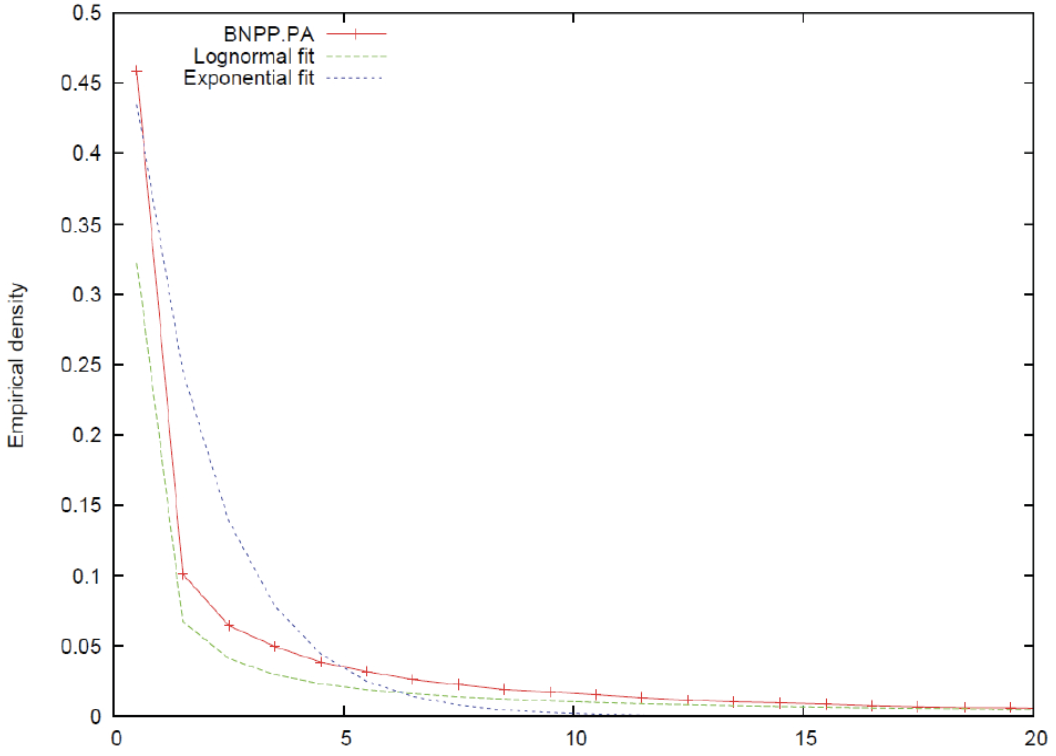
\includegraphics[width=0.9\textwidth]{chapters/chapter_trade_data_models/figures/intertime.png} 
   	\caption{Distribution of inter-arrival times of market orders for stock BNPP.PA (Chakraborti et al. 2011). \label{fig:intertimefig}}
	\end{figure}

The use of Poisson processes to model the flows of limit orders, market orders and cancellations makes the method analytically tractable. The model captures the steady-state shape of the order book (although there may be other distributions that may be fit better besides Poisson, see Figure~\ref{fig:intertimefig}) but it may not be useful for predicting short-term behavior that may be more relevant for the traders. The assumption of Poisson process results in that the intensity of arrivals and cancellations does not depend on the state of the order book which is somewhat unrealistic given the feedback loop relationship between the behavior of the market participants and the history of the order book. Recent works, by Zhao (2010)~\cite{} and Abergel (2010)~\cite{} show that the memory-less property is not empirically valid. Orders tend to be clustered due to dependencies between liquidity taking and liquidity providing and also due to algorithmic execution of parent order that is split into numerous child orders. Also, the assumption that all orders are of the same size is too simplistic. 


Zhao (2010)~\cite{} proposes a model based on marked point process when the mark represents order types, price, size etc.. The joint modeling also assumes that the order flow is self-exciting, i.e. new orders or cancellations occur in an orderly point processes with an intensity function that depends on the history of the limit order book. The model is somewhat difficult to estimate and does not fully capture the empirical results such as volatility clustering etc.. \\

\noindent\textbf{Hawkes Process:} The features of volatility clustering and the significant autocorrelations in durations between order arrivals and significant cross-correlation of arrival rates across various event types are better captured by multi-dimensional Hawkes process. For a given $M$-dimensional point process, let $N_t=(N_t^1,\ldots,N_t^M)$ denote the associated counting process and the Hawkes process is characterized by intensities, $\lambda^m(t), m=1,\ldots,M$ as
	\begin{equation}\label{eqn:lambdamdoub}
	\begin{split}
	\lambda^m(t)&= \lambda_0^m(t) + \sum_{n=1}^M \int_0^t \sum_{j=1}^P \alpha_j^{mn} e^{-\beta_j^{mn}(t-s)} dN_s^n \\
	&=\lambda_0(t) + \sum_{n=1}^M \sum_{t_j<t} \sum_{j=1}^P \alpha_j^{mn} e^{-\beta_j^{mn}(t_j -t_i^n)}
	\end{split}
	\end{equation}
where the number of exponent kernels, $P$, is fixed and $t_i^n$ is the $i$th jumping time of the $m$th variate. The scale and decay parameters, $\alpha^{mn}$ and $\beta^{mn}$ express the influence of the past events $t_i^n$ of type `$n$'. The baseline model in (\ref{eqn:lambdamdoub}) does not incorporate the effect of bid-ask spread on order flow. It is shown in Anderson, Cont and Vinkovskaya (2010)~\cite{} that $\alpha$ and $\beta$ parameters do depend on the bid-ask spread. A simulated Hawkes process is given in Figure~\ref{fig:hawkes}. The main characteristic of the Hawkes process is that intensity goes up at each event and decays exponentially between events. 
	\begin{figure}[!ht]
   	\centering
   	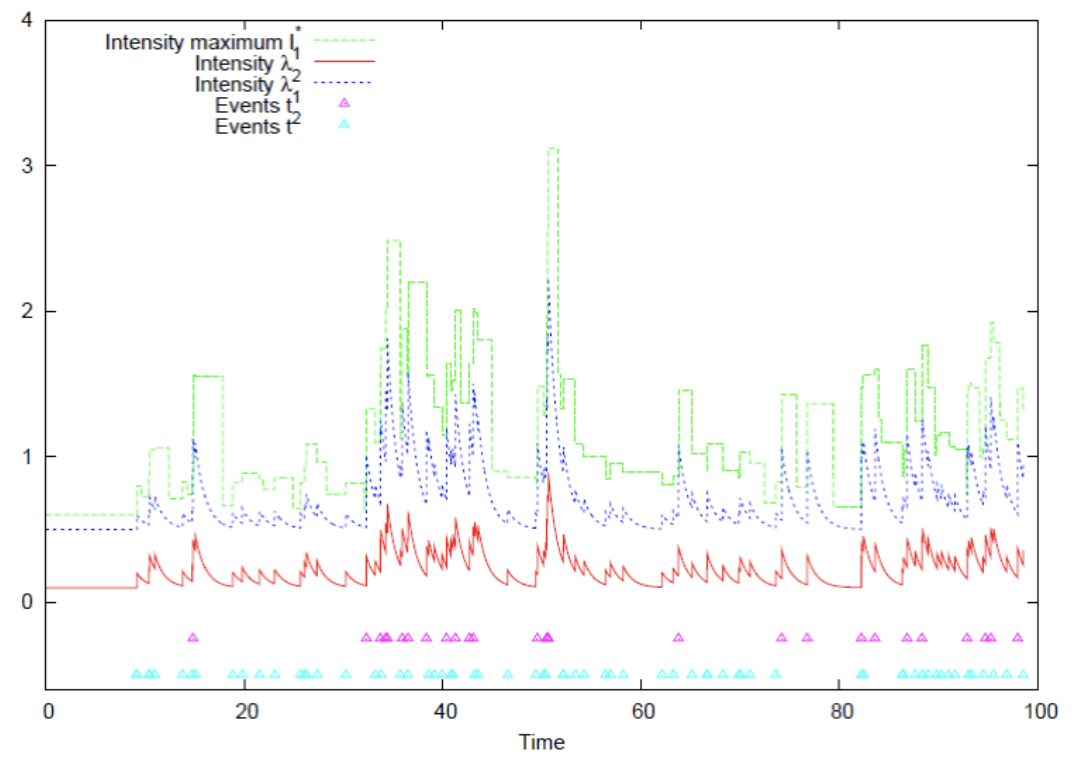
\includegraphics[width=0.9\textwidth]{chapters/chapter_trade_data_models/figures/hawkes.png} 
   	\caption{Simulated two-dimensional Hawkes process (Toke 2011). \label{fig:hawkes}}
	\end{figure}

The evolution of the order book is driven by six different intensity functions, but the model changes with the value of the spread. The base intensity and the decay rates are all assumed to be functions of the spread. The model is quite complex and requires the estimation of a large number of parameters, which in turn requires vast amount of data for calibration. 


The mathematical framework was developed in Hawkes (1971)~\cite{} and was expanded in Hawkes and Oakes (1974)~\cite{}. The application of Hawkes process in finance is of recent origin: see Toke (2011)~\cite{} or Bacry et al. (2011)~\cite{}. We will briefly discuss the likelihood estimates of the model in (\ref{eqn:lambdamdoub}). First, we want to observe for a Poisson process, the intensity function $\lambda(t)=\lambda_0$, a constant. The log-likelihood of the model,
	\begin{equation}\label{eqn:loglikemod}
	\ln \mathcal{L}(\{t_i\}_{i=1,2,\ldots,N}) = \sum_{m=1}^M \ln \mathcal{L}^m(\{t_i\})
	\end{equation}
where
	\[
	\ln \mathcal{L}^m(\{t_i\})= T - \sum_{i=1}^N \sum_{n=1}^M \dfrac{\alpha^{mn}}{\beta^{mn}} (1- e^{-\beta^{mn}(T-t_i)}) + \sum_{t_i^m} \ln[ \lambda_0^m(t_i^m) + \sum_{n=1}^M \alpha^{mn} R^{mn}(l) ]
	\]
and 
	\[
	R^{mn}(l)= \sum_{t_\kappa^n t_l^m} e^{-\beta^{mn}(t_l^m-t_\kappa^n)}
	\]
is the cumulative decay function. Using the Multiplicative Random Time Change Theorem (see Meyer (1971)~\cite{}) that states that with a certain transformation of the variables, the Hawkes process can be changed to a unit rate homogeneous Poisson process. Transforming the time variable `$t$' into `$\mathcal{T}$', where
	\begin{equation}\label{eqn:calt}
	\mathcal{T}= \int_0^t \lambda(s) \; ds
	\end{equation}
Hawkes process becomes a Poisson process with unit rate. Thus
	\begin{equation}\label{eqn:diffcalt}
	\mathcal{T}_i - \mathcal{T}_{i-1}= \Lambda(t_{i-1},t_i) = \int_{t_{i-1}}^{t_i} \lambda(s) \; ds
	\end{equation}
is exponentially distributed. 


More generally in the `$M$' dimensional multivariate case,
	\[
	\begin{split}
	\Lambda^m(t_{i-1}^m,t_i^m)&= \int_{t_{i-1}^m}^{t_i^m} \lambda_0^m(s) \; ds + \int_{t_{i-1}^m}^{t_i^m} \sum_{n=1}^M \sum_{t^n<t_{i-1}^m} \alpha^{mn} e^{-\beta^{mn}(s-t^n)} \; ds \\
	&+ \int_{t_{i-1}^m}^{t_i^m} \sum_{n=1}^M \sum_{t_{i-1}^m<t^n<s} \alpha^{mn} e^{-\beta^{mn}(s-t^n)} \; ds
	\end{split}
	\]
will follow exponential distribution. The $\Lambda^m(t_{i-1}^m,t_i^m)$ are known as compensators and can be verified empirically if it follows exponential distribution. 


\subsection{Application of a Hawkes process}


We want to illustrate the model with an application. We will first look at the statistical properties of the data and then look at the results of fitting one and two dimensional Hawkes processes to it. Our findings show that a two dimensional model based on Hawkes processes performs considerably better than a model based on two independent Poisson Processes. This provides strong evidence of the fact that the two key features of Hawkes processes (path dependency of the order flow and the possibility of modeling the interaction between the dimensions) are capable of capturing and replicating some of the key features of the empirical data. Moreover, there is evidence of significant and asymmetric interplay between the buy and the sell sides for the Limit Orders and evidence of limited interplay between the two sides when it comes to Market Orders. Finally, a study of the statistical properties of the orders showed a complex of alternating symmetric and asymmetric behavior of the LOB. 


The data at hand is INET data for XOM (Exxon Mobil) for the 1st of September 2010. The first step was to look at the submission frequency of the Limit Orders during the trading day. Figure~\ref{fig:freqsubmitarrivals} shows such frequency plot and we can see how in the first hour a half and in the last half an hour of the trading day there is a much higher submission frequency (with peaks of 25/30 orders submitted per second) than during the rest of the day (around 5--10 orders per second).
	\begin{figure}[!ht]
   	\centering
   	\includegraphics[width=0.75\textwidth]{chapters/chapter_trade_data_models/figures/freqsubmit.png} 
   	\caption{Frequency of Limit Order submission for 09/01/2010 (time in minutes after market opening). \label{fig:freqsubmitarrivals}}
	\end{figure}


This means that if we choose to look at the Limit Order flow with a model that doesn't allow for a varying baseline intensity, we will have to drop these two periods of increased trading activity and keep the data for only the middle portion of 6 hours of the trading day.


We then looked at the data for the central portion of 6 hours of the trading day and found that market orders are just a function of Limit Orders. There were almost 90,000 Limit Orders submitted during that period of the day, compared to the only about 4,000 Market Orders. Similarly, there is an imbalance in the side of the order submission, with around 42,000 Limit Orders submitted on the Sell side compared to the 48,000 submitted on the Buy side (about 18\% more). This side-imbalance is also present in the Market Order submission although not that strongly: 1,882 Market Orders submitted on the Sell side compared to the 2,107 orders submitted on the Buy side (only about 12\% more). 
	\begin{table}
	\centering
	\caption{XOM data for 09/01/2010 \label{tab:xom}}
	\begin{tabular}{llll} 
	& Limit Orders & Market Orders & Total \\ \hline
	Buy & 48,541 & 2,107 & 50,648 \\ 
	Sell & 41,194 & 1,882 & 43,076 \\
	Total & 89,735 & 3,989 & 93,724
	\end{tabular}
	\end{table}
This shows how, on this trading day, most of the ``action'' was occurring on the Buy Side of the book which could mean that the markets were confident in an increase of the price of XOM (in line with the historical performance of the stock for that day).


Our next step was to re-construct the Limit Order book from the order flow so to look at the life of the Limit Orders after their submission. We first looked into how many of the submitted Limit Orders get executed and, when they do, in how many fills. We found Table~\ref{tab:LOexec} that only about 6.5\% of all submitted LOs get at least partially filled with the percentage dropping to only about 6\% for those LO that actually get completely executed. Also, out of the LO that are completely filled nearly 90\% of them is filled in just one execution. This allows us to say that the magnitude of the LOs is comparable to that of the Market Orders, given that nearly all of them require only one Market Order to fill it completely. It is also interesting to note how few of the LOs that are submitted actually get executed. 
	\begin{table}
	\centering
	\caption{LO executions and percentage breakdown by number of fills required \label{tab:LOexec}}
	\begin{tabular}{cccc}
	Number of LO & \% at least partially fill & \% completed in one fill & \% completely fill \\
	89, 735 & 6.57 & 5.35 & 6.15
	\end{tabular}
	\begin{tabular}{ccccccc}
	1 & 2 & 3 & 4 & 5 & 6 & $\geq$ 7 \\ \hline
	87.14 & 10.83 & 1.34 & 0.37 & 0.13 & 0.06 & 0.13
	\end{tabular}
	\end{table}


This means that either very few LO are actually submitted close to the market (hence have a chance to get executed) or that many of them don't stay in the book long enough to get executed. This led us to look into the life-time of the LOs and, more specifically, at their cancellation and execution times. We focused on how long, on average, for an order to be either not filled or partially filled LO stayed in the book before getting cancelled and at how long did it take for a LO to be either filled for the first time or completely filled. Results are given in Table~\ref{tab:meanlo}.
	\begin{table}
	\centering
	\caption{Mean LO cancellation and execution times (in seconds) \label{tab:meanlo}}
	\begin{tabular}{cccc}
	\multicolumn{2}{c}{No Fills} & \multicolumn{2}{c}{Partial Filles} \\ \hline
	Buy Orders & Sell Orders & Buy Orders & Sell Orders \\ \hline
	177.8 & 250.5 & 46.1 & 63.0 \\ \hline
	\multicolumn{2}{c}{First Fill} & \multicolumn{2}{c}{Completion} \\ \hline
	 25.3 & 56.2 & 25.6 & 57.6
	\end{tabular}
	\end{table}

In this particular case, LOs stay in the book for much longer if they are on the sell side than if they are on the buy side. Orders that have never been filled are cancelled after 250 seconds if they are on the sell side compared to 177 seconds if they are on the buy side. Similarly, a partially filled LO on the sell side is cancelled after 63 seconds compared to 46 seconds if it's on the other side of the book. Also, if we look at the time it takes for a LO to be filled for the first time we see that that happens after about 56 seconds on the sell side compared to only 25 seconds on the buy side. Finally, for the LO that do get completely filled, it takes on average 1 minute for that to happen if the order is on the sell side compared to only 25 seconds if the order is on the buy side. This life-time difference for LOs on the two opposite sides of the book is consistent with what we saw earlier in the imbalance of the LO and MO submission. In fact, in this case as well we see how the buy side appears to be the more active side of the book. The shorter execution times for the orders on the buy side could be caused by either more aggressive pricing or by the price movements of the markets while the shorter lifespans and the higher number of orders on that side seem to indicate the use of more active trading strategies. However, there is another interesting observation that can be made. We see that on average a sell LO that is filled for the first time (but that doesn't get completely filled), is cancelled after about 7 seconds, compared to the 20 seconds that it would take had the order been on the buy side. This means that on average it takes three times longer for a partially (and never completely) filled order to be cancelled if it is on the buy side (which is the more active side) that if it is on the sell side (which is the less reactive side). The asymmetry between buy and sell side at the aggregated level has been noted in the literature.


The next step was to observe changes in the behavior of the book when moving further away from the market. We looked into the order submission and cancellation frequencies as a function of distance from the market price. Figure~\ref{fig:canfreq} and Figure~\ref{fig:freqsubmit1} show that most LO are submitted and cancelled at the market (respectively, 40\% and almost 30\%) and that the rates drop sharply with each price level further away from it. This supports the conclusion that the very small percentage of executed LO is not caused by the fact that most LO are submitted far away from the market and hence don't get the chance to get executed. We can also see how approximately 70\% (96\%) of all Limit Orders is placed in the top 5 (20) levels of the book and that 69\% (96\%) of all cancellations also occurs in the top 5 (20) levels. This a first indication of the fact that Level III data offers more information than Level II since with the top 5 levels of the book we were only able to capture around 70\% of all the occurring events. However, this also indicates that there is no need to use all the information provided in Level III data since by looking at only the top 20 levels of the book we are still able to capture nearly all of the occurring events. Both plots show a very similar behavior for the buy and sell side which led us to assume an almost symmetric behavior of the book. This assumption was later tested and confirmed at a 99\% confidence level with a two-sided Kolmogorov-Smirnov Test. 
	\begin{figure}[!ht]
   	\centering
   	\includegraphics[width=0.75\textwidth]{chapters/chapter_trade_data_models/figures/subfreqnear.png} 
   	\caption{Submission frequencies--Distance near touch price \\ Kolmogorov-Smirnov Test Statistics$=0.61 \to$ fail to reject null at 1\% sig. level \label{fig:subfreqnear}}
	\end{figure}
	\begin{figure}[!ht]
   	\centering
   	\includegraphics[width=0.75\textwidth]{chapters/chapter_trade_data_models/figures/canfreqnear.png} 
   	\caption{Cancellation Frequencies--Distance from near touch price \\ Kolmogorov-Smirnov Test Statistic$=0.83\to$ fail to reject null at 1\% sig. level \label{fig:canfreqnear}}
	\end{figure}


Better understanding what happens to the LOs once they enter the book is key in developing a more accurate way of choosing when to submit a LO or a MO. For this reason we also looked at the cancellation frequencies as a function of position in the queue and we found that (Figure~\ref{fig:canfreq}) most of the cancellations occur when the LO are in 4th or 5th position in the queue. In this case as well, we carried out a test of the assumption of a symmetric behavior of the book which confirmed previous similar findings. However, it would be more interesting to look at the cancellation frequencies as a function of overall distance from the market (as a measure of distance from possible execution). 
	\begin{figure}[!ht]
   	\centering
   	\includegraphics[width=0.75\textwidth]{chapters/chapter_trade_data_models/figures/canfreq.png} 
   	\caption{Cancellation Frequencies---position in queue. \label{fig:canfreq}}
	\end{figure}


With two more trading days (3rd and 9th of September 2013) data available, we are able to study the robustness of the above results. The submission and cancellation frequencies as a function of relative price which were symmetric for the 1st of September were not symmetric anymore on the 3rd of September. In this trading day, Figure~\ref{fig:freqsubmit1}, the peak of activity on the buy side occurred 12 price levels away from the market. This seems to suggest that on the 3rd of September the markets were betting that the price of XOM would drop in the foreseeable future, possibly reacting to some new event. A closer investigation of that time period revealed in the previous days the announcement by Exxon Mobil of the plan of closing a refinery which then led to a drop in the price shortly after 09/03/2010.
	\begin{figure}[!ht]
   	\centering
   	\includegraphics[width=0.75\textwidth]{chapters/chapter_trade_data_models/figures/losubcanfreq.png} 
   	\caption{LO submission and cancellation frequencies. \label{fig:losubcanfreq}}
	\end{figure}


A second interesting difference was in the amount of volume on the two sides of the book (Figure~\ref{fig:losubcanfreq}). Across the 3 days there was a significant volume imbalance with considerably more volume on the sell side than on the buy side but the amount of imbalance between the two sides changes significantly across the three days. Overall there is no explanation as to why there would be such a strong volume imbalance in favor of the sell side other than some kind of temporary anomaly. These findings seem to point out the fact that the shape and behavior of the LOB change dramatically across different days and that, in order to capture some kind of more general/average behavior of the book, many more days of data are required. 
	\begin{figure}[!ht]
   	\centering
   	\includegraphics[width=0.75\textwidth]{chapters/chapter_trade_data_models/figures/freqsubmit.png} 
   	\caption{Frequency of Limit Order submission for 09/01/2010 (time in minutes after market opening). \label{fig:freqsubmit1}}
	\end{figure}
	\begin{figure}
	\centering
	\begin{subfigure}
	  \centering
	  \includegraphics[width=.4\linewidth]{chapters/chapter_trade_data_models/figures/timevol1.png}
	\end{subfigure}%
	\begin{subfigure}
	  \centering
	  \includegraphics[width=.4\linewidth]{chapters/chapter_trade_data_models/figures/timevol1.png}
	\end{subfigure}
	\caption{Frequency of Limit Order submission for 09/01/2010 (time in minutes after market opening). \label{fig:freqsubmit2}}
	\end{figure}


\subsection{One-Dimensional Models}


We started by building a one dimensional model for the Limit Orders submitted on the buy side and one for those submitted on the sell side. Similarly, we build a one dimensional model for the Market Orders submitted on each side of the book. In the one dimensional case, the intensity function driving the Hawkes process is of the form
	\begin{equation}\label{eqn:lambda6}
	\lambda(t)= \lambda_0 + \alpha \sum_{t_i<t} e^{-\beta(t-t_i)}
	\end{equation}
with $\lambda_0$ indicating the baseline intensity, $\alpha$ indicating the jump in the intensity after the occurrence of an event and $\beta$ indicating the rate of exponential decay of the intensity after the occurrence of an event.


Table~\ref{tab:limmodbuy} and Table~\ref{tab:limmodsell} show the results of the MLE estimation of the parameters of the one dimensional models for the Limit Orders on the two sides of the book. The difference in the values of the estimates of the parameters for the two sides of the book (strongest on the 9th and weakest on the 1st of September) indicates that there is a level of asymmetry between these two sides. Also, even though the magnitude of the values of the parameters is the same for all three days (on each side of the book) there is still some variation between them, especially when we look at the model for the buy side. This seems to suggest that the behavior of the book can change considerably from day to day and that a considerable amount of data might be necessary in order to capture some kind of general behavior. 
	\begin{table}
	\centering
	\caption{1-D Limit Order Model (buy side) \label{tab:limmodbuy}}
	\begin{tabular}{c|ccc} 
		& $\lambda$ & $\alpha$  & $\beta$ \\ \hline
	09/01/2010 & 0.008108431 & 1.421767060 & 1.435094466 \\
	09/03/2010 & 0.006127003 & 1.290012415 & 1.299564704 \\
	09/09/2010 & 0.002341542 & 1.023410145 & 1.026757239
	\end{tabular}
	\end{table}
	\begin{table}
	\centering
	\caption{1-D Limit Order Model (sell side) \label{tab:limmodsell}}
	\begin{tabular}{c|ccc} 
		& $\lambda$ & $\alpha$ & $\beta$ \\
	09/01/2010 & 0.002055786 & 1.071071139 & 1.073989940 \\
	09/03/2010 & 0.002342963 & 0.983678355 & 0.986999404 \\
	09/09/2010 & 0.006123845 & 0.946420813 & 0.955774394
	\end{tabular}
	\end{table}


One of the advantages of having chosen an exponential decay for the intensity function of the process, becomes apparent when we analyze the meaning of these parameters. Using a well-known property of exponentially distributed variables, we can tell the half-life of the excitation effect caused by the occurrence of an event. In the specific, in our one-dimensional models we find that, on average, half of the excitation effect caused by the occurrence of an event is dissipated after about 0.7 seconds ($\frac{\ln 2}{\beta} \approx$ half-life). Also, the small estimated values for $\alpha$ indicate that the occurrence of an event has a very small impact on the likelihood of another event occurring. This seems to suggest that there is a weak self-excitation effect in the LO process when modeling it with a one-dimensional model. 


We then build, in a similar fashion, the two one-dimensional models for the flow of buy and sell Market Orders for all three days and obtained the following parameter estimation: 
	\begin{table}[!ht]
	\centering
	\caption{1-D Market Order Model (buy side) \label{tab:marketorderbuy}}
	\begin{tabular}{c|ccc} 
		& $\lambda$ & $\alpha$ & $\beta$ \\ \hline
	09/01/2010 & 0.0238743 & 7.3187478 & 19.8477514 \\
	09/03/2010 & 0.01450873 & 3.38168999 & 7.70581048 \\
	09/09/2010 & 0.0267254 & 4.8818834 & 13.5427254
	\end{tabular}
	\end{table}
	\begin{table}[!ht]
	\centering
	\caption{1-D Market Order Model (sell side) \label{fig:marketordersell}}
	\begin{tabular}{c|ccc} 
		& $\lambda$ & $\alpha$  & $\beta$ \\ \hline
	09/01/2010 & 0.02083999 & 9.38842281 & 24.55777564 \\
	09/03/2010 & 0.01616096 & 6.64370599 & 16.68090519 \\
	09/09/2010 & 0.0239992 & 8.2180945 & 25.0115980
	\end{tabular}
	\end{table}
The first thing that is obvious is the asymmetry between the buy and the sell sides. Nevertheless, for the Market Orders they asymmetry appears to be much more significant that it was for the Limit Orders, given the much bigger differences in the values of the estimated parameters. Also, for Market Orders we see that the occurrence of each event seems to have a much stronger impact on the likelihood of occurrence of future events than it was the case for Limit Orders. In fact, the values of $\alpha$ in Table~\ref{tab:marketorderbuy} and Table~\ref{fig:marketordersell} are considerably higher than those we saw in Table~\ref{tab:limmodbuy} and Table~\ref{tab:limmodsell}. Similarly, the values of $\beta$ are also much larger in the Market Order models than they were in the Limit Order models which means that the half-life of the excitation effect is much shorter for Market Orders (0.03 seconds vs. 0.7 seconds) than for Limit Orders. These differences in the results of the estimations are not that surprising if we consider what we saw in Table~\ref{tab:xom} for order submissions. Market Orders are submitted in much fewer numbers than Limit Orders which explains why even though the occurrence, such self-excitation has a very short lifetime. The significant increase in the chances of another Market Order occurring given that one has just occurred (even through for a very short time), might seem contradicting the fact that very few Market Orders actually occur. However, what can be inferred is that Market Orders depend strongly from the occurrence of other Market Orders and that they tend to cluster around submissions. 


\subsection{An extension}


An important limitation of this basic Hawkes Process model is that each event has the same impact on the intensity function. This implies that each event carries the same amount of information in the process. However, it is easy to imagine that a large LO would carry much more information about future price changes than a small one and this should be accounted for in the model. We include order size in the intensity function by scaling the size of the jump $\alpha$ in the value of the intensity by the ratio $\frac{w_i}{\overline{w}_l}$, where $w_i$ is the size of the LO and $\overline{w}_l$ is the average LO size up to that point. The intensity function for this ``extended'' one-dimensional model becomes
	\[
	\lambda(t)= \lambda_0 + \alpha \sum_{t_i<t} \dfrac{w_i}{\overline{w}_l} e^{-\beta(t-t_i)}
	\]
We then compared the performance of this ``size-adjusted'' model with the ``basic'' one by using the before mentioned \emph{Multivariate Random Time Chance} Theorem and looking at the Q-Q plot of the compensators for the two models. Figure~\ref{fig:lobuysideadj} and Figure~\ref{fig:losellsideadj} show how in both case (buy and sell Limit Orders) adjusting for size doesn't improve the fit of the model. This result is somewhat counter-intuitive given that more than 70\% of all Limit Orders are of size 100 shares and that this should imply that any deviation from this size explanation is that trading strategies are successful in concealing the true intension of the traders and that there is no significant information left in the size of the LO once that the strategies are implemented and the orders are submitted. 
	\begin{figure}[!ht]
   	\centering
   	\includegraphics[width=0.75\textwidth]{chapters/chapter_trade_data_models/figures/lobuysideadj.png} 
   	\caption{LO--buy side with size adjustment and without. \label{fig:lobuysideadj}}
	\end{figure}
	\begin{figure}[!ht]
   	\centering
   	\includegraphics[width=0.75\textwidth]{chapters/chapter_trade_data_models/figures/losellsideadj.png} 
   	\caption{LO--sell side with size adjustment and without. \label{fig:losellsideadj}}
	\end{figure}


\subsection{Two-Dimensional models}


Our next step was to build two-dimensional models that would simultaneously model the buy and sell sides of the book and with two separate (yet interacting) intensity functions. The intensity functions for this kind of model become
	\[
	\begin{split}
	\lambda^B(t)&= \lambda_0^B + \int_0^t \alpha^{BB} e^{-\beta^{BB}(t-u)} \;dN_u^B + \int_0^t \alpha^{BB} e^{-\beta^{BS}(t-u)} \;dN_u^S \\
	\lambda^S(t)&= \lambda_0^S + \int_0^t \alpha^{SB} e^{-\beta^{SB}(t-u)} \; dN_u^B + \int_0^t \alpha^{SS} e^{-\beta^{SS}(t-u)} \;dN_i^S
	\end{split}
	\]
and we have 5 parameters for each dimension of the model for a total of 10 parameters across the two dimensions (buy and sell). The two additional parameters in each dimension account for the cross-excitation effect between the two dimensions. In our case, $\alpha^{BS}$ tells us the increase in the likeliness of a LO occurring on the buy side after the occurrence of a LO on the sell side, while $\beta^{BS}$ tells us the rate of decay of the buy side intensity after the occurrence of a LO on the sell side (and vice-versa for $\alpha^{SB}$ and $\beta^{SB}$). We then used MLE to estimate the parameters of the model and we can make several remarks about the results (Table~\ref{tab:2dimlomodel}).
	\begin{table}
	\centering
	\caption{2-Dimensional LO model \label{tab:2dimlomodel}}
	\begin{tabular}{lllll}  
	$\lambda^B=2.480 \cdot 10^{-5}$ & $\alpha^{BB}=14.386$ & $\beta^{BB}=31.517$ & $\alpha^{BS}=0.303$ & $\beta^{BS}=0.464$ \\ \hline
	$\lambda^S=2.677 \cdot 10^{-5}$ & $\lambda^{SS}=15.657$ & $\beta^{SS}=37.299$ & $\alpha^{SB}=0.149$ & $\beta^{SB}=0.312$ \\ 
	\end{tabular}
	\end{table}
	
	
There appears to be some asymmetry in the cross-excitation effects with the occurrence of an event on the sell side having a stronger impact on the likeliness of occurrence of an event on the buy side rather than the other way round ($\alpha^{BS}>\alpha^{SB}$). On the other hand though, since $\beta^{BS}<\beta^{SB}$, the effect on the sell side of an occurrence on the buy side is more persistent than that of an event on the buy side on the sell side (2.22 seconds vs. 1.49 seconds).
	\begin{figure}[!ht]
   	\centering
   	\includegraphics[width=0.75\textwidth]{chapters/chapter_trade_data_models/figures/asymcross.png} 
   	\caption{Asymmetry in cross-excitation effect. \label{fig:asymcross}}
	\end{figure}
The self-excitation components of the model are rather similar for both dimensions and it is interesting to point out the very short persistence of the self-excitation effect in both cases (about 0.02 seconds).


In order to evaluate whether the two key features of a model based on Hawkes processes (path dependency of the order flow and the possibility of modeling the relation between the various dimensions) are really helpful in improving the performance of the model, we decided to compare the performance of our model to that of a bi-dimensional model based on two independent Poisson Processes (which by definition of Poisson process cannot account for any dependency in the order flow and by construction assume independence between the two dimensions). The results proved to be very encouraging with a remarkably better fit to the empirical data for the Hawkes Process based model (Figure~\ref{fig:4hawkes6}).
	\begin{figure}[!ht]
   	\centering
   	\includegraphics[width=0.75\textwidth]{chapters/chapter_trade_data_models/figures/4hawkes6.png} 
   	\caption{Top--Fit of Hawkes Process (buy \& sell); Bottom--Fit of Poisson Process (buy \& sell). \label{fig:4hawkes6}}
	\end{figure}


Following a similar procedure, we build a bi-dimensional model for the Market Orders and performed MLE to estimate the parameters. The results (Table~\ref{tab:2dimmomod}) showed very weak and symmetric cross-excitation between the dimensions which, however, turns out to be very persistent (141 seconds for the half-life of the effect of buy on sell and 215 seconds for that of sell on buy). The self-excitation effect is comparable across the two dimensions and is also very short lived (with a half-life of about 0.02 seconds).
	\begin{table}
	\centering
	\caption{2-Dimensional MO model \label{tab:2dimmomod}}
	\begin{tabular}{lllll}  
	$\lambda^B=2.701 \cdot 10^{-5}$ & $\alpha^{BB}=11.793$ & $\beta^{BB}=36.153$ & $\alpha^{BS}=0.0037$ & $\beta^{BS}=0.0049$ \\
	$\lambda^S=3.451 \cdot 10^{-5}$ & $\alpha^{SS}=12.454$ & $\beta^{SS}=35.063$ & $\alpha^{SB}=0.0017$ & $\beta^{SB}=0.0032$
	\end{tabular}
	\end{table}
	

Finally, we compared the performance of our model to that of the bi-dimensional Poisson Process. Similarly to the LO case, the model at hand significantly outperforms the Poisson Process one for both dimensions. 
	\begin{figure}[!ht]
   	\centering
   	\includegraphics[width=0.75\textwidth]{chapters/chapter_trade_data_models/figures/4fig.png} 
   	\caption{Top--Fit of Hawkes Process (buy \& sell); Bottom--Fit of Poisson Process (buy \& sell). \label{fig:4fig6}}
	\end{figure}


\subsection{Limitations and findings}


There are some important considerations to be made based on our analysis. The first issue is related to the cleaning of the data that was necessary in order to adapt it to our needs. In fact, Hawkes processes are ``simple'' processes which means that they don't allow for more events to occur simultaneously. Unfortunately, in the INET data it is quite common to encounter clusters of 10/20 events reported with the same timestamp. This is typical of high frequency data due to the approximation with which events are often reported and to the obvious limitation of the chosen time scale (e.g., milliseconds). In our case we decided to keep only the first event of each cluster, dropping all the others. A possible alternative used in the literature is to simply uniformly distribute the events from the clusters across the time interval given by the occurrence of the cluster and that of the next event. However, this approach could introduce bias in the parameter estimation phase. In fact, the clustering of events by itself is of interest.


Also, an important limitation of the bi-dimensional Hawkes Process model is that it is very computationally intense. Evaluating the 5 parameters for one of the two intensity function using data from only one trading day took almost 48 hours. It becomes clear that in order to evaluate the parameters of a model using data for a longer time period of if evaluating the parameters for a model with higher dimension (hence with more parameters) will require considerably more computational power. 

\section{Models for Hidden Liquidity}

\section{Supplements and Problems} 


% !TEX root = ../../book.tex
%\hfill
%\par\vspace{\baselineskip}

\chapter{Market Impact Models}
\section{Overview of Market Impact Models}

One of the main focuses of Algorithmic Trading is minimizing costs of trade execution. When a large order is executed in the market, it causes market impact (MI), which is commonly defined as the deviation of the post-trade market price from the market price that could have prevailed had the trade not occurred (Fabozzi, Focardi and Kolm (2006)~\cite{ffk}). To alleviate MI and the implied transaction cost (TC), a trader may use an algorithmic trading system to slice a large ``parent'' order into a sequence of ``child'' orders. While a slicing strategy is typically motivated by the liquidity constraint associated with executing a large order in one print, it is usually balanced against the risk and opportunity costs associated with the execution of a sequence of child orders over a longer duration as discussed earlier.


In asset management, with the competitive focus of the industry on cost management and diminishing returns of crowded strategies, understanding and managing MI has become a crucial component of a systematic investment process. For an estimate of its size among the transaction costs that include explicit costs such as brokerage commissions and fees, see Table~\ref{tab:empttrans} from Berkovec and Heidle (2010)~\cite{borkoheidle}. Managing MI has important implications on three aspects of algorithmic trading: pre-trade TC estimation, post-trade TC analysis and the design of optimal trading strategies (Almgren (2008)~\cite{alm2008}).

\begin{table}[!ht]
	\caption{Empirical Transaction Cost Estimates$^1$ \label{tab:empttrans}}	
		\begin{tabular}{|c|c|c|}
		Type & Fixed & Variable\\ \hline
		\hline
		Explicit & Commissions (7.4bp) & Bid-ask spreads (1.9bp)\\ \hline
		& Fees & Taxes\\ \hline
		\hline
		Implicit & & Delay Cost (9.5bp)\\ \hline
		 & & Price Movement Risk \& \\
		 & & Market Impact Costs* (35.6bp)\\ \hline
		 & & Timing Risk \& Opportunity Costs (11.7bp)\\ \hline 
		\end{tabular}
\small *Major Component \\ 1: Readers should note changes in the market that have taken place since these numbers were reported. The commissions are quite expensive for current trading. Most developed markets  have commissions less than 1~bps, while E.M. markets are in the range of 2--5~bps for e-trading. The bid-ask spread makes sense if it is half a spread of liquid U.S. stocks. For other markets, it can be much higher.  \normalsize
\end{table}


The study of price impact dates back to Bagehot (1971)~\cite{} who postulated that the market consists of heterogeneously informed traders. The specialist cannot distinguish between informed and uninformed (liquidity) traders and fixes a spread that can balance the trading cost. The asymmetric information models based on this notion have been extensively studied in finance literature. The traders do convey information and Hasbrouck (1991)~\cite{hasbrouk} provides empirical evidence that the market maker can infer information from the characteristics of the sequence of trades. The seminal work by Kyle (1985)~\cite{kyle1985} and Huberman and Stanzl (2004)~\cite{huberstan} indicate that an order of large size (parent order) must be sliced into a number of small order (child orders) so that the volume per se will not signal informed trading. The hypothesis that time between the trades could convey the information flow (Easley and O'Hara (1992)~\cite{easleyo}) and its impact on price is studied in Dufour and Engle (2000)~\cite{dufour}. Long durations are usually associated with no new news and the variations in trading intensity are taken to be positively correlated with the behavior of the informed traders. \\


\noindent \textbf{Origins of Market Impact:} Most conventional definitions of the MI of a trade equate it with the deviation of the post-trade market price from the market price that would have prevailed had the trade not occurred. Figure~\ref{fig:marketimpt} shows an idealized MI picture of $n$-share sell order from Fabozzi, Focardi and Kolm (2006)~\cite{ffk} but Figure~\ref{fig:detmarketimpt} is augmented to include other information: (1) the state of the order book establishes a pre-trade equilibrium, (2) this equilibrium is disturbed by a market order to sell n shares, (3) as the sell order depletes the bid order book, it obtains an increasingly lower trade price and results in the trade print, and, (4) over time the price gradually moves up back to recover some of the price drop. Accordingly, the difference between (4) and (3) is called temporary impact, whereas the difference between (4) and (1) is called permanent impact. If we are looking to model the MI effect of sequential trades, as shown in Figure~\ref{fig:marketimpt}, the temporary and permanent impact will be superpositions of those of individual trades. The permanent impact is often assumed to be immediate and linear in the parent trade size, and the post-trade equilibrium to be the same for the order of n shares or a sequence of m orders of n/m shares each (Almgren et al. (2005)~\cite{athl}; Fabozzi et al., (2006)~\cite{ffk}). By contrast, the temporary impact is a function of how the ``parent'' trade is split into smaller ``child'' trades.
	\begin{figure}[!ht]
	\centering
	\includegraphics[width=\textwidth]{chapters/chapter_exec_models/figures/fig1ab.jpg}
	\caption{Idealized MI Model: single sell trade (left) and entire parent sell trade (right). \label{fig:marketimpt}}
	\end{figure}
The mechanisms responsible for the permanent and temporary impacts have been a subject of significant interest. One common view links price changes accompanying large trades to the information cost and liquidity cost (Chan and Lakonishok (1995)~\cite{chan1995}; Holthausen et al. (1990)~\cite{holthausen1990}) potentially attributed to any transaction. In terms of information cost, the market response to the fact that a market participant has decided to sell (buy) shares of a particular stock could be perceived as conveying new (private) information about the fundamentals of a security (e.g., firm's management, debt conditions) and thus its future prices. Consequently, it results in a permanent price change with no price reversals. In terms of liquidity cost, the market response to the fact that liquidity was removed out of the order book can be perceived as the effect of distorting the liquidity demand/supply equilibrium. The consequence is a temporary price impact that dissipates soon after the trading occurs, at a speed that depends on the market ability to absorb liquidity demand.


Independent of the market microstructure responsible for MI, two central concerns to much theoretical and empirical work are the functional form (shape) of the MI and the key determinants of this form. As seen in Figure~\ref{fig:detmarketimpt}, MI is influenced by trade-related factors (e.g., relative trade size, time of trade), asset-specific factors (e.g., market capitalization, shares outstanding, bid-ask spread) and exchange- and market-related factors (e.g., liquidity, trading volume, institutional features). Models that incorporate these factors tend to be more complex but with better predictive power.
	\begin{figure}[!ht]
	\centering
	\includegraphics[width=\textwidth]{chapters/chapter_exec_models/figures/fig2.jpg}
	\caption{Determinants of Market Impact. \label{fig:detmarketimpt}}
	\end{figure}
Numerous stylized MI models offer some insight into the possible shapes of the permanent and temporary impact functions. Some of these models focus only on the permanent impact, while some models also attempt to capture the effect of temporary impact. \\


\noindent \textbf{Equilibrium Permanent Impact Models:} Models of one class, including Kyle's (1985)~\cite{kyle1985} and Hubberman and Stanzl's (2004)~\cite{huberstan}, rest on the efficient market hypothesis positing that all available information is included in prices. These models use a time-independent framework to establish an equilibrium price after a trade is executed. This means that trades are assumed to have only a permanent price impact (Huberman and Stanzl, 2004, p. 1260)~\cite{huberstan}


Under these settings, Huberman and Stanzl (2004)~\cite{huberstan} show that, if no quasi-arbitrage possibilities exist (to ensure viable markets), the permanent impact must be linear in the trade quantity and symmetric between buys and sells. Linearity in trade size has been established by Kyle (1985)~\cite{kyle1985} as well. In fact, Huberman and Stanzl (2004)~\cite{huberstan} add that ``Nonlinear, time-dependent price-update functions may assume ``chaotic'' shapes without giving rise to price manipulation. Only when additional assumptions are made on the shapes of these functions does the analysis become meaningful.''


Almgren et al. (2005)~\cite{athl} develop a different market impact model, in the context of finding an optimal execution strategy for a large trade [see the discussion of Almgren and Chriss model in Section 7.1.2] that is sliced into several smaller trades. They describe the random process satisfied by the stock price using an arithmetic Brownian process that depends directly on a permanent impact function that is linear in trade size and therefore has no effect on the optimal execution strategy. However, they recognize that if the total number of units traded is sufficiently large, the execution price may steadily change between trades, in part because the supply of liquidity is exhausted at each successive price level. They assume that this effect is short-lived because liquidity returns after each period and a new equilibrium price is established. They model this effect using a temporary price impact function that is non-linear in trade size. They then postulate that both the permanent and temporary impact functions follow power laws based on theirs' and others' empirical results. (Loeb (1983)~\cite{loeb}; Lillo, Farmer and Mantegna (2003)~\cite{farmermantegna}). \\


\noindent \textbf{Hybrid Impact Models:} Models of another class assume that trading agents have zero intelligence (instead of being fully rational) and take random decisions to buy or to sell, but that their action is interpreted by all the others agents as containing some potential information. The mere fact of buying, or selling typically leads to a change of the ask $a$, or bid $b$, price and hence to a change of the midpoint $p=\frac{a+b}{2}$. The new midprice is also expected to follow a random walk (at least for sufficient large times), if it is immediately adopted by all other market participants as the new reference price around which new orders are launched.


Madhavan et al. (1997)~\cite{madhaven1997} develop a price formation model postulating that the (bid-ask) mid price `$p$' changes because of unpredictable public information shocks (news) and microstructure effects that include statistical effects of order flow fluctuations (e.g., autocorrelation) and trading frictions (e.g., asymmetric information, dealer costs). This postulate automatically removes any predictability in the price returns and ensures market efficiency. If all trades have the same volume and the surprise component of the order flow at the $k$th trade is given by $\epsilon_k - \rho \,\epsilon_{k-1}$, where the signs of trades $\epsilon_n$ are generated by a Markov process with correlation $\rho$,\footnote{This means that the expected value of $\epsilon_k$ conditioned on the past only depends on $\epsilon_{k-1}$, given by: $E(\epsilon_k\,|\,\epsilon_{k-1})=\rho\,\epsilon_{k-1}$.}  one writes the following evolution equation for the midprice as:
	\begin{equation}\label{eqn:midpointdelta}
	\Delta p_{k+1}=p_{k+1}-p_k=\theta[\epsilon_k - \rho \epsilon_{k-1}]+\eta_k
	\end{equation}
where $\eta$ is the shock component and the constant $\theta$ measures the size of trade impact. Empirical estimation of their model are not aimed at investigating the shape of impact functions.\footnote{First, both information flows and trading frictions are important factors in explaining intraday price volatility in individual stocks. Second, information asymmetry decreases steadily throughout the day, however, dealer costs increase over the day (possibly reflecting the costs of carrying inventory overnight) so that bid-ask spreads exhibit the U-shaped pattern commonly noted in previous research studies.}


Others extend the model of Madhavan et al.~(1997) to gain insight into the shape of impact functions.  Bouchaud et al. (2009)~\cite{bouchaud2009} use (\ref{eqn:midpointdelta}) to compute several important quantities. Principally, they write the lagged return impact function (for time points $n$ and $n+l$), denoted $R_l$, as:
	\begin{equation}\label{eqn:rlittlel}
	R_l = p_{n+l}-p_n = \theta \sum_{j=n}^{n+l-1}[\epsilon_j - \rho \epsilon_{j-1}]+ \sum_{j=n}^{n+l-1}\eta_j
	\end{equation}
and then show that the lagged impact function is constant and equal to:
	\begin{equation}\label{eqn:rlittlel2}
	R_l = \theta (1-\rho^2), \forall l
	\end{equation}
Now define the ``bare'' impact of a single trade taken at time $l$, denoted $G_0(l)$, which measures the influence of a trade at time $n-l$ on the bid-ask midprice at time $n$. Written in terms of $G_0(l)$, the midpoint process is expressed as:
	\begin{equation}\label{eqn:plittlen}
	p_n = \sum_{j=-\infty}^{n-1}G_0(n-j-1)\,\epsilon_j + \sum_{j=-\infty}^{n-1}\eta_j
	\end{equation}
Then it can be shown that $G_0(0) = \theta$ and $G_0(l) = \theta(l-\rho)$ for $l>0$. Bouchaud et al. (2009)~\cite{bouchaud2009} also observe that ``The part $\theta \rho$ of the impact instantaneously decays to zero after the first trade, whereas the rest of the impact is permanent. The instantaneous drop of part of the impact compensates the sign correlation of the trades.''


Bouchaud et al. (2004)~\cite{bouchaud2004} have developed an earlier price evolution model, similar to (\ref{eqn:rlittlel}), where the price at time $n$ is written as a sum over all past trades of the impact of one given trade propagated up to time $n$:
	\begin{equation}\label{eqn:anotherplittlen}
	p_n = \sum_{n'<n} G_0(n-n')\,\epsilon_{n'} \ln{V_{n'}} + \sum_{n'<n} \eta_{n'}
	\end{equation}
where $V_n$ denotes the volume of a trade at time n and $G_0()$ is assumed to be a fixed non-random function that only depends on time differences. The $\eta_n's$ are also random variables, assumed to be independent from $\epsilon_n$, and are used to model all sources of price changes not described by the direct impact of the trades. The authors then consider constraints imposed on the shape of response function, $G_0$, by three empirical results they discuss: (a) the midprice price process is close to being purely diffusive, even at the trade-by-trade level; (b) the temporal structure of the impact function first increases and reaches a maximum after some number (100 to 1000) of trades, before decreasing back with a rather limited overall variation; and the sign of the trades shows surprisingly long-range, power-law correlations. These empirical results are reconciled with (\ref{eqn:anotherplittlen}) by assuming that the response function $G_0()$ must instead also decay as a power-law in time, with an exponent precisely tuned to ensure simultaneously that prices are nearly diffusive and that the response function is nearly constant. Gatheral (2010)~\cite{gatheral}, assuming that the trading costs should be non-negative, demonstrates that the exponential decay of market impact is compatible only when the market impact is taken to be linear. Thus the debate on the functional form of MI is ongoing. 


It has been noted that the models developed to study market impact generally do not consider situations that may arise from strategies where price impact may depend upon the state of the order book. The second generation models consider the behavior of the limit order book. Hautsch and Huang (2012)~\cite{hauthuang} consider a time-aggregated model. The activities in the book are captured in Table~\ref{tab:vardef} and the market depth is kept to the three best quotes on both sides of the market.
	\begin{table}[!ht]
	\centering
	\caption{Model (\ref{eqn:7dy}) Variable Definitions \label{tab:vardef}}
	\begin{tabular}{ll}
	Variable & Description \\ \hline
	$p_t^a$ & Logarithm of the best ask after the $t$-th event. \\
	$p_t^b$ & Logarithm of the best bid after the $t$-th event. \\
	$v_t^{a,l}$ & Logarithm of the market depth at the $l$-th best ask after the $t$-th event. \\
	$v_t^{b,l}$ & Logarithm of market depth at the $l$-th best bid after the $t$-th event. \\
	$\text{BUY}_t$ & Dummy equal to one if the $t$-th event is a buyer-initiated trade. \\
	$\text{SELL}_t$ & Dummy equal to one if the $t$-th event is a seller-initiated trade. 
	\end{tabular} 
	\end{table}
Let $Y_t$ be a $K$-dimensional listing the variables in Table~\ref{tab:vardef}; the co-integration model in Chapter 2 is fit for the data:
	\begin{equation} \label{eqn:7dy}
	\Delta Y_t = \mu + \alpha \beta' y_{t-1} + \sum_{t=1}^{p-1} \Gamma_i \Delta Y_{t-i} + u_t
	\end{equation}
The co-integrating $(K \times r)$ matrix, $\beta$ has first two columns restricted to have entries as zeros except for buy and sell indicators. To study the market impact, the model is written in the reduced-form to capture the impulse-response coefficients as:
	\begin{equation}\label{eqn:7largeyt}
	Y_t = \mu + \sum_{i=1}^p A_i Y_{t-i} + U_t
	\end{equation}
where $A_1=I_k+\alpha\beta' + \Gamma_1$, $A_i=\Gamma_i - \Gamma_{i-1}$ for $1<i<p$ and $A_p= -\Gamma_{p-1}$. The $\text{VAR}(p)$ model in (\ref{eqn:7largeyt}) can then be written in the form of $\text{VAR}(1)$ as 
	\begin{equation}\label{eqn:starlargeyt}
	Y_t^*= \mu^* + A^* Y_{t-1} + U_t^*
	\end{equation}
where $\mu^*=(\mu',0',\ldots,0')'$, $Y_t^*=[Y_t',Y_{t-1}',\ldots,Y_{t-p+1}']$, $U_t^*=[U_t',0',\ldots,0']'$ and $A^*=\renewcommand\arraystretch{1.3} \mleft[ \begin{array}{c|c} A_1\cdots A_{p-1} & A_p \\ \hline I_{K(p-1)} & 0 \end{array} \mright]$. It can be shown that 
	\begin{equation}\label{eqn:7anotherlargeyt}
	Y_t= JM_t + \sum_{i=0}^{t-1} JA^i J' U_{t-i}
	\end{equation}
where $J=[I_k,0,\cdots,0]$ is a $k\times kp$ selection matrix and $M_t= A^{*t} Y_0^* + \sum_{i=0}^t A^{*i}U_{t-i}^*$.

Recall that the market impact measures the impact of current trade on the future trades; it is measured by the impulse response function
	\begin{equation}\label{eqn:impulserep}
	f(h,\delta_h) = E[y_{t+h}\,|\, y_t+\delta_y,t_{t-1},\cdots] - E[y_{t+h} \,|\, y_t,y_{t-i},\cdots] = JA^{*h} J' \delta_y
	\end{equation}
where $\delta_y$ is the change to $Y_t$, due to the current trade. The long-run effect, $f(\delta_y)=C \delta_y$, where $C=\beta_\perp(\alpha_\perp'(I_K - \sum_{i=1}^{p-1} \Gamma_i ) \beta_\perp )^{-1} \alpha_\perp'$. Here $\alpha_\perp$ and $\beta_\perp$ are orthogonal to $\alpha$ and $\beta$ in (\ref{eqn:7dy}).


Hautsch and Huang (2012)~\cite{hauthuang} estimate the market impact using the data from Euronext, Amsterdam for heavily traded stocks. The main findings are, besides the existence of co-integrating relationships between quotes and depths, limit orders have long-term effects on quotes, the price movement is influenced by the order size and the decrease of spreads after the arrival of a limit order is reverted back asymmetrically soon after. The between-stock variations in market impact are shown to be related to trading frequency of the stocks. 


Cont, Kukanov and Stoikov (2014)~\cite{contkulst} consider the dynamics of market liquidity that is a function of limit orders, market orders and cancellations to model the price impact function. The outstanding limit orders provide a measure of depth in the market on both buy and sell sides and thus also provide a measure of order flow imbalance (OFI).


By setting the number of shares (depth) or price levels beyond the best bid and ask is equal to $D$, define the price change in the interval $(t_{k-1},t_k)$ as,
	\begin{equation}\label{eqn:doubleeq}
	\begin{split}
	\Delta P_k^b&= \delta \left[ \dfrac{L_k^b - C_k^b - M_k^s}{D} \right] \\
	\Delta P_k^s&= -\delta \left[\dfrac{L_k^s-C_k^s-M_k^b}{D}\right]
	\end{split}
	\end{equation}
where $L_k^i$, $C_k^i$ and $M_k^i$ for $i=b,s$ denote arrival of the limit orders, cancellations and market orders in the defined interval. Here $\delta$ is the tick size. If $P_k=\dfrac{P_k^b+P_k^s}{2\delta}$, that is mid-price normalized by tick size, for any $s$nd-interval, $(t_{k-1,i},t_{k,i})$, it is postulated that
	\begin{equation}\label{eqn:postulated}
	\Delta P_{k,i} = \beta_i \text{OFI}_{k,i} + \Eulerconst_{k,i}
	\end{equation}
where $\text{OFI}_k=(L_k^b-C_k^b-M_k^s)-(L_k^s-C_k^s-M_k^b)$ and $\Delta P_k=\frac{\text{OFI}_k}{2D}+\epsilon_k$. Here it is important to note that `$\beta_i$' is taken to be price impact coefficient and is taken to be inversely proportional to market depth:
	\begin{equation}\label{eqn:7betai}
	\beta_i=\dfrac{C}{D_i^\lambda} + v_i
	\end{equation}
The models in (\ref{eqn:postulated}) and (\ref{eqn:7betai}) can be regarded to represent instantaneous price impact. The model as it can be seen from the set-up assumes that all activities in the limit order book have an average linear impact, $\beta_i$, in the $i$th interval. 


Cont et al. (2014)~\cite{contkulst} using the TAQ data for a month in 2010 for fifty stocks estimate the model in (\ref{eqn:postulated}) over ten-second intervals. The model is generally confirmed by the data with $\hat{\beta}_i$ is significant in most of the samples and $\hat{\alpha}_i$ is only significant in less than twenty percent of the samples. It must be noted that there is a significant number of trades posted gets cancelled within a few seconds of submission. Various theories that are postulated (see Hasbrook and Saar (2009)~\cite{habbrooksaar}) are yet to be fully empirically tested. Hence instead of using OFI, trade imbalance $(\text{TF}_k=M_k^b-M_k^s)$ is used in equation (\ref{eqn:postulated}). Results are still reasonable, but not as strong as using OFI in the model. Finally the relationship between $\hat{\beta}_i$ and $D_i$ (price impact coefficient and depth) is studied; the results indicate for model (\ref{eqn:7betai}), $\hat{C} \sim 0.5$ and $\hat{\lambda} \sim 1$. Some interesting conclusions that could be useful for trading are drawn. The impact coefficient varies more with the amount of liquidity provision (OFI) than the trade imbalance (TI). It can be also used to monitor adverse selection. If a limit order is filled after a positive OFI, price is likely to go up and for a limit sell order, a positive change would imply that the order was executed at a loss. These conclusions need to be firmed up with further studies in this area. \\


\noindent\textbf{Determinants of Empirical relationship:} A key aspect of MI modeling is to provide information about expected pre-trade costs. The studies that have been reviewed on empirical analysis thus far can help us to understand how the price formation and the market impact function evolve during a trading period. But most clients who want to trade large quantities of equities want to know the trading costs apriori. Here we review the relevant studies and augment with our own research in this area. First we review the factors that are found to influence these costs in block trades. Although block trades differ in fundamental ways to algorithmic, they can be treated as all equivalent to a parent trade except that no splitting into child orders occurs.


\begin{itemize}
\item \textbf{Trade Size.} Many studies observe that the (relative) size of trades positively relates to the magnitude of MI (Keim and Madhavan (1996)~\cite{madhavan}), consistent with the prediction of stylized model (Kyle (1985)\cite{kyle1985}; Huberman and Stanzl (2004)~\cite{huberstan}).

\item \textbf{Market Capitalization.} Keim and Madhavan (1996)~\cite{keim1996}find that the asymmetry of trading costs between buys and sells is more pronounced among smaller stocks. This is consistent with what is broadly known to be the effects of market capitalization on MI (Lillo et al. (2003)~\cite{farmermantegna}; Chan and Lakonishok (1997)~\cite{chan1997}). From a practical point of view, market cap itself may not be a true factor but it can be a proxy for some liquidity characteristics. 

\item \textbf{Price Volatility.} Price volatility has been found to be positively related to MI (Chiyachantana et al. (2004)~\cite{chiya2004}). One explanation is that elevated volatility is associated with greater dispersion in beliefs, with risk averse traders less inclined to participate in markets, thereby resulting in greater price concessions or MI (Domowitz et al. (2001)~\cite{domo2001})

\item \textbf{Trading Activity.} Dufour and Engle (2000, p. 2467)~\cite{dufour} find that the price impact of trades increases as the time duration between transactions decreases, and more broadly that the price impact is especially large due to increased trading activity, as measured by high trading rates. In their view, ``times when markets are most active are times when there is an increased presence of informed traders; we interpret such markets as having reduced liquidity.'' Likewise, Yang (2011, p. 91)~\cite{yang2011} finds that ``a trade shortly after the previous trade results in higher price impact than one after a long period.'' He also offers ``evidence that increased trading activity (as measured by short durations between trades) is associated with larger price impact, therefore implying a higher degree of information-based trading.''

\item \textbf{Time of Day.} It is reported that the MI for buy trades decreases as time passes during the day, with the highest impact in the first trading hours (Frino et al. (2007)~\cite{frino}).
\end{itemize}


We will now summarize briefly the models that are used in the industry. For many years, traders have used the simple sigma-root-liquidity model described for example by Grinold and Kahn (1994)~\cite{grin2000}. The model takes the form,
	\begin{equation}\label{eqn:spreadcost}
	\Delta P - \text{Spread Cost} = \alpha\cdot\sigma\sqrt{\frac{X}{V}}
	\end{equation}
where $X$ is the size of the parent order, $V$ is the average daily volume and `$\sigma$' is the volatility of the stock. Thus the relative size (RS), $\frac{X}{V}$ is the key factor in the pre-trade cost estimation and the impact is proportional to volatility. The square root of relative size is expected because risk capital should be proportional to the square-root of the holding period. In Toth et al. (2011)~\cite{toth2011anomalous}, the authors present an argument that if latent supply and demand are linear in price over some plausible range of prices, which is a reasonable assumption, market impact should be square-root.


The square-root formula as stated in (\ref{eqn:spreadcost}) refers only to the size of the trade relative to daily volume. It does not refer to for example, the rate if trading, how the trade is executed and the market capitalization of the stock. If the trading is quite aggressive, the square-root formula tends to break down. Moro et al (2009)~\cite{moro2009market} observe that the price path during the execution follows a power law:
	\begin{equation}\label{eqn:ptalpha}
	p_t - p_0 = \alpha\cdot({\frac{t}{T}})^{2/3}
	\end{equation}
where $T$ is the duration of the parent-order. Immediately after completion of a parent-order, the price begins to revert. Other models used in industry are mostly functions of the determinants identified above. \\


\noindent\textbf{Select Empirical Studies:} While there is some discussion about the theoretical models for market impact, published studies based on large scale data are somewhat rare especially when it comes to models useful for pre-trade cost estimation, Almgren et al (2005)~\cite{athl} took US stock trade orders processed by Citigroup for Dec 2001 - June 2003 and estimated a model of the market impact as given in Table~\ref{tab:costimpact}. For two select stocks, IBM and DB, the power law model for market impact are estimated. The temporary impact is defined as $\widetilde{p}_k - p_{k-1}$, for $k^{th}$ execution. The model depends on relative size, inverse turnover ratio, which is the number of the shares outstanding to average daily volume and the volatility.


While the square root formula in (\ref{eqn:spreadcost}) is quite robust and holds even beyond equity markets, recent empirical studies confirm the need for more general power law functions; the quotient of $\text{RS}=\frac{X}{V}$ varies depending on other factors that get included in the model (refer to the estimates in Table~\ref{tab:costimpact} for RS). Zarinelli, Treccani, Farmer and Lillo (2015)~\cite{zar} show that logarithmic functional form fits the data better for the large order data that they consider. 


\begin{table}[!ht]
\caption{Example of impact costs (Almgren et al. (2005)~\cite{athl} \label{tab:costimpact}}
\begin{tabular}{cccc}
 & & IBM & DRI \\ \hline
Average daily volume & $V$ & 6.561~m & 1.929m~ \\
Shares outstanding & $\theta$ & 1728~m & 168~m \\
Inverse turnover & $\theta/V$ & 263 & 87 \\
Daily volatility (\%) & $\sigma$ &1.57 & 2.26 \\
Normalised trade size & $X/V$ & 0.1 & 0.1 \\ \hline
Normalised permanent & $l/\sigma$ & 0.126 & 0.096 \\
Perm. price impact (bp) & $l$ & 20 & 22 \\ \hline
Trade duration (days) & $T$ & 0.1 \hspace{0.2cm} 0.2 \hspace{0.2cm} 0.5 & 0.1 \hspace{0.2cm}0.2 \hspace{0.2cm} 0.5\\
Normalised temporary & $K/\sigma$ & 0.142 \hspace{0.2cm} 0.094 \hspace{0.2cm}0.054 & 0.142 \hspace{0.2cm} 0.094 \hspace{0.2cm} 0.054 \\
Temp. Impact cost (bp) & $K$ & 22 \hspace{0.2cm} 15 \hspace{0.2cm} 8 & 32  \hspace{0.2cm}21\hspace{0.2cm} 12 \\ \hline
Realised cost (bp) & $J$ & 32 \hspace{0.2cm} 25 \hspace{0.2cm} 18 & 43 \hspace{0.2cm}32 \hspace{0.2cm} 23
\end{tabular}
\small Note: examples of permanent and temporary impact costs are shown, for a purchase of 10\% of the day's average volume, in two different large-cap stocks. The permanent cost is independent of time of execution. The temporary cost depends on the time, but across different assets it is the same fraction of daily volatility (from Almgren et al. (2005)~\cite{athl}). \normalsize
\end{table}


Limited access to broker-proprietary algorithmic trading data has stifled detailed academic inquiry in this area. While the impact of algorithmic trading is extensively discussed in the finance literature, formal empirical results are rare. The few exceptions we are aware of are: Engle et al (2012)~\cite{engle2012}, who use proprietary algorithmic trading data from Morgan Stanley to study the risk-return tradeoff associated with increasing the number of child trades and duration of parent trade; Domowitz and Yegerman(2005)~\cite{doye}, who use ITG's Transaction Cost Analysis Peer Group Database to compare execution costs for a set of 40 buy-side clients; and Hendershott and Riordan (2011)~\cite{hernderrio}, who use algorithmic trading data from firms listed on the Deutsche Boerse DAX to measure the contribution of algorithmic trading to price discovery. A few academic studies resort to using proxies based on publicly-available TAQ data. Two examples are: Hendershott et al. (2011)~\cite{hender2011}, who use NYSE electronic message traffic data as a proxy for algorithmic liquidity supply to study how algorithmic trading effects liquidity and bid-ask spreads; and Chaboud et al. (2014)~\cite{chaboud}, who use FX quote data (highest bid and lowest ask) from an electronic limit order book platform called EBS to construct mid-quote series for studying the effect of algorithmic trading on FX rates' volatility. The use of mid-point prices, in the lack of actual arrival price and completion price for a parent trade, has been criticized for failing to capture the possible asymmetry of the bid and ask price impacts of trading, which has been observed to exist for block trades. In any event, none of these studies deals with the estimation of MI models per-se.


Velu, Gretchika, Benaroch, Nehren and Kuber (2015)~\cite{unpub} address these issues using a large algorithmic trading dataset provided by J.P. Morgan Chase. The data contain ``parent'' algorithmic executions, including the initial arrival price and fill price as well as the child trades' average fill price (computed as the share-weighted average executing price of the child orders). The algorithmic executions are generated using Volume Weighted Average Price (VWAP) and Percent of Volume (POV) strategies.Recall the volume weighted average price (VWAP) strategy schedules to trade some constant percentage of the expected market volume regularly throughout the day, where the proportion traded is adjusted based on historical market volume profiles and the predict volume. Hence, in VWAP, the trading schedule is predetermined based on a prediction of the daily market volume distribution, although the timing of executions may be randomized so as to make the trading pattern less predictable. By contrast, the percent of volume (POV) strategy trades a fixed percentage of the current market volume where the trading schedule is dynamically determined based on a historical analysis of volume profiles used to anticipate trading volumes. Unlike implementation shortfall strategies, VWAP and POV do not explicitly take into account the expected MI in generating their algorithmic executions. Moreover, although firms typically implement proprietary versions of these strategies with parameters reflecting their experience and clients' profiles, VWAP and POV nonetheless generate relatively standardized algorithmic executions. In other words, from the perspective of MI, these two strategies can be safely considered ``plain vanilla'' in the sense that firm-to-firm differences in their behavior and performance are too insignificant. The measures employed, therefore, do not depend on any unique traits of the strategies. The unique aspect of the data is that if the meta order is on the buy side or sell side is explicitly provided. 


The dataset allows us to study the effect of parent characteristics on the market impact and the implied transaction cost (TC). Specifically, we estimate the parameters of a family of power-law models, investigate the explanatory power of different determinants of market impact and TC, and develop insights useable for pre-trade cost estimation. Our model estimation effort is informed by existing stylized market impact models and empirical findings about the market impact of block trades. These stylized models are reviewed earlier in this section. In addition to studying the effects of buy and sell trades, order size, price volatility and market cap, we examine the effect of the number of child trades and duration of the parent trade. Lastly, we also summarize two extensions of our model estimation effort that pertain to the effect of the bid-ask spread on market impact and to the market impact of ETFs traded via algorithmic trading.


This study has some important findings. A central novel insight that emerges from the analysis is that market impact can be substantially decreased by reducing the number of child order trades. There could be several explanations, but a simple plausible one is that reducing the number of child trades reduces the information leakage about trading intentions. This explanation is in line with the main premise of Farmer et al. (2012)~\cite{farmer2012} that, in an efficient market, market impact is determined by the information that is disseminated through trades. It is also consistent with studies showing that the price impact is larger as the duration between trades decreases and there is increased trading activity (Dufour and Engle 2000~\cite{dufour}; Yang 2011~\cite{yang2011}), and that the number of trades may drive prices more than the actual trade size (Jones et al. 1994~\cite{jones1994}).


Another finding is the nuanced difference in market impact and TC that is related to buy and sell trades. On the overall level, this difference is statistically significant, and this presumably contradicts the buy-sell market impact asymmetry commonly reported for block trades. However, a deeper examination reveals a more nuanced difference between buy and sell trades. Visual inspection of the TC vs. trades' relative size and the TC vs stocks market cap shows that in some sub-ranges there is a difference between buys and sells. After dividing trades into 24 bins based on their relative size and testing the TC difference within each bin we observe that the difference is statistically significant in six bins; six out of 24 exceeds the proportion expected when testing multiple hypotheses at a 5\% significance level. Consequently, separate market impact and TC models for buy and the sell trades are estimated, and observed the following about the difference between the coefficients of buys and sells. This difference is significant in models containing a subset of the explanatory factors (e.g., relative size alone, or relative size and volatility), but it is within a two standard errors threshold in models containing all the factors. Our findings notwithstanding, it is necessary to investigate further whether the underlying causes may be linked to the specifics of trade flow, the logic behind many of the trading algorithms.


It is important to mention two caveats . One relates to the role of permanent versus temporary impact in our analysis. The data set does not contain information about the price dynamics after the completion of the parent trades, that is, only completion price for the last child order is available. Therefore, it was not possible to determine what portion of the measured market impact is permanent and what portion of it is temporary. Another caveat relates to the high variability in the data. To obtain a better signal out of the noisy data, the data was smoothed through binning and extraction of key descriptives. The models are based on these descriptives. Nevertheless, for robustness testing all models were estimated using the raw unsmoothed data and the results are qualitatively similar, albeit the $R$-square values are understandably much lower. \\


\noindent\textbf{Empirical Details: } The market impact is modeled as a non-linear function of several stock-related and trade-related factors. The power law form is generally recommended for non-linear shape. The data analyzed in Velu et al. (2015)~\cite{unpub} consists of over 250,000 parent orders fully executed over a one-year period, Oct 1, 2009--Sept 30, 2010. All trades were completed within a single trading day. Each parent trade was sliced into multiple child trades; each child trade was executed in one or several partial fills. Only parent trades executed through widely used VWAP (volume-weighted average price) or POV (percent of volume) strategies (Brandes et al. (2007)~\cite{brandes2007}). This ensures that the participation rate is well-defined and stays roughly constant over the duration of the parent trade. We define 
	\small
	\[
	\text{Market Impact (MI) in bps }= \text{side } \cdot \left(\dfrac{\text{\small Completion Price} - \text{\small Arrival Price}}{\text{\small Arrival Price}}\right) \cdot 10000
	\]
	\[
	\text{Transaction Cost (TC) in bps}= \text{side } \cdot \left(\dfrac{\text{\small Average filled Price }-\text{ \small Arrival Price}}{\text{\small Arrival Price}} \right) \cdot 10000
	\]
\noindent \normalsize where the arrival price is the price when the first child order is executed and completion price is the price when the last child order is executed. Every trade in this data is explicitly identified as buy or sell. This contrasts with studies that use TAQ data that do not have the same explicit identification. Using Lee and Ready (1991)~\cite{leeready} heuristic rule to determine the trade direction can be sometimes inaccurate (Asquith, Oman and Safaya (2011)~\cite{asquith2010} and Chakrabarty, Moulton and Shkilko (2012)~\cite{chakrabarty2012short}). To make the analysis robust, we binned the explanatory variables and obtained smoothed averages; the analysis is based on binned data.


Results start with a visual inspection of the relationships. The graphs clearly indicate that the relationship between MI and RS is non-linear, and it remains non-linear with binning of other factors as well. The relationship between MI and relative size is monotonic till the relative size reaches 20\% or so (Figure~\ref{fig:oneoffive}).Trades with longer durations clearly have a lower MI (Figure~\ref{fig:twooffive}). Trades for higher volatility stocks, too, can be read to have a higher MI (Figure~\ref{fig:threeoffive}). Trades on larger market cap stocks have a smaller MI (Figure~\ref{fig:fouroffive}). Lastly, MI becomes higher as the number of child trades increases (Figure~\ref{fig:fiveoffive}). This last relationship is important and deserves special attention particularly when designing execution strategies. There is a clear trade-of between low ``immediate'' liquidity impact of small child orders and long term information leverage of the parent order level when hitting the market too frequently. But the power law model is more general and can accommodate interaction effects as well. These graphs for various factors besides RS can be collapsed into a master curve, with appropriate normalization, as given in Lillo et al. (2003)~\cite{farmermantegna}.
	
	
	\begin{figure}[!ht]
	\centering
	\includegraphics[width=\textwidth]{chapters/chapter_exec_models/figures/fig3.jpg}
	\caption{MI vs. RS. \label{fig:oneoffive}}
	\end{figure}

	\begin{figure}
	\centering
	\includegraphics[width=\textwidth]{chapters/chapter_exec_models/figures/fig4.jpg}
	\caption{MI vs. RS and Duration. \label{fig:twooffive}}
	\end{figure}

	\begin{figure}
	\centering
	\includegraphics[width=\textwidth]{chapters/chapter_exec_models/figures/fig5.jpg}
	\caption{MI vs. RS and Volatility. \label{fig:threeoffive}}
	\end{figure}

	\begin{figure}
	\centering
	\includegraphics[width=\textwidth]{chapters/chapter_exec_models/figures/fig6.jpg}
	\caption{MI vs. RS and Market Cap. \label{fig:fouroffive}}
	\end{figure}

	\begin{figure}
	\centering
	\includegraphics[width=\textwidth]{chapters/chapter_exec_models/figures/fig7.jpg}
	\caption{MI vs. RS and No. of Children. \label{fig:fiveoffive}}
	\end{figure}


Table~\ref{fig:marketimpt} shows the results of power-law models ; the standard errors are shown in parentheses below the estimated regression coefficients. All coefficients in the models presented in Table~\ref{fig:marketimpt} are statistically significant. This is consistent with Almgren et al. (2005)~\cite{athl}, except that in their model the market-cap-to-volume ratio is not significant. It should be noted that the values of $R$-square are significantly higher than other published studies, mainly due to binning and smoothing. The response variable is not an individual parent trade cost, but rather the average cost for trades in a bin representing a combination of various levels of predictors. Thus, the models developed here are intended to predict the average MI for a combination of predictors.


\begin{table}[!ht]
\caption{Response Variable is MI (bps) ($\hat{\sigma}^2=225, n=2,$ 211 bins)}
\begin{tabular}{|c|c|c|c|c|c|c|}
Predictor & Model 1& Model 2 & Model 3 & Model 4 & Model 5 & Model 6* \\ \hline
Rel. Size & 0.53 & 0.51 & 0.56 & 0.63 & 0.43 & \\
	& (0.02) & (0.02) & (0.02) & (0.02) & (0.02) & \\
Volatility & & 1.12 & 0.92 & 1.17 & 0.53 & \\
	& & (0.09) & (0.09) & (0.11) & (0.1) & \\
Duration	& & & $-0.24$ & $-0.25$ & $-0.47$ & $-0.27$ \\
	& & & (0.02) & (0.02) & (0.3) & (0.1) \\
Market Cap & & & & $-0.09$ & $-0.12$ & $-0.04$ \\
	& & & & (0.02) & (0.02) & (0.07) \\
No. of Children & & & & & 0.53 & 0.55 \\
	& & & & & (0.04) & (0.16) \\
Constant & 9.6 & 19.6 & 15.9 & 9.4 & 2.7 & 1.3 \\
	& (0.34) & (1.07) & (0.9) & (1.3) & (0.46) & (1.3) \\
\hline
$\hat{\sigma}_{\text{error}}^2$ & 143 & 136 & 125 & 124 & 114 & N/A \\
$R^2$ & 0.37 & 0.40 & 0.45 & 0.45 & 0.50 & 0.03 \\
\end{tabular}
\small*Response Variable$ = \frac{\text{MI}(\text{bps})}{(\text{Vol})(\text{RS})^0.6}$\normalsize
\end{table}


Several relevant observations can be made about the coefficients in the estimated models. For example, Model 3, which is traditionally well cited in the literature, can be written as:
	\[
	\text{MI(bps)}= 15.9\cdot\sigma^{0.92}\cdot(RS)^{0.56}\cdot T^{-0.24}
	\]
Note that the volatility coefficient is approximately `one' and the coefficient of RS is about 0.5 has indeed been observed in the literature. It is consistent with the folklore that it takes one day's volatility to trade one day's volume. The duration effect is also consistent as most of the parent trading occurs in less than two hours in the data set, not always in real life. This has led us to consider an additional model where $\frac{MI(bps)}{(Vol)(RS)^{0.6}}$ is used as a normalized response variable. This variable can be taken as the multiplicative residual term of  Model (2) in Table~\ref{fig:marketimpt}.The regression results of this variable on other variables are given under Model (6*). Two observations can be made: the duration and the number of child trades are still significant factors. However. The increase in $R$-square is somewhat smaller than the unrestricted versions of the same model, labeled as Model (5) in Table~\ref{fig:marketimpt}.


Other key findings can be summarized as follows:

\begin{itemize}
\item Relative size and volatility consistently exhibit positive influences on MI; their impact varies depending on other factors in the model.

\item Duration has an inverse effect. Its use in the model must be carefully calibrated as the execution of parent trades using child trades can be highly concentrated.

\item Stocks with higher market capitalizations tend to have smaller price impact for the same relative size.

\item The number of child trades, which is usually determined by the trading algorithm, does reveal a positive effect on MI.
\end{itemize}

There are several practical considerations that may limit the use of these model for pre-trade cost estimation. These challenges in MI calibration is due to the following facts:
	\begin{enumerate}[--]
	\item Not enough data for certain combinations of the factors involved.
	
	\item MI is a noisy measure which is hard to calibrate ex-post.
	
	\item Sometimes, market moves at a much larger magnitude than MI.
	
	\item Use of raw data results in a poor predictive models; thus a need for aggregation. But aggregation obviously ignores the wide variation within the aggregated unit. 
	\end{enumerate}

% !TEX root = ../../book.tex

\chapter{Modeling Execution Strategies}

While algorithmic trading techniques are useful in both low and high frequency settings, their importance has become more pronounced in the age of electronic trading because of the speed in execution and the necessity for efficient matching of demand and supply sides in the limit order books. Added to this is that modern equity markets where order submission and cancellations are automated are also highly fragmented with dozens of exchanges and about forty alternative trading systems where investors can choose to trade. The trading algorithms differ over various types of market participants, but all of them try to optimize dynamically where, how often and at what price to trade. Typically, the execution layers can be broadly described as follows (see Gatheral (2012)\cite{}):
	\begin{itemize}
	\item \textbf{The Macrotrader:} Given a meta-order (parent trade) translate the objective function of a strategy into a trading schedule; when the algorithm should trade, in what size (child order) and for how long.
	\item \textbf{The Microtrader:} Given a slice (child order) of the meta-order to trade, this layer of algorithm decides whether to place it as a market or as a  limit order and at what price level.
	\item \textbf{The Smart Order Router:} For a given order (quantity and price level) to which venue should the order be sent.
	\end{itemize}


In this chapter we discuss these and other execution issues in the high frequency trading context. Generally the objectives of equity trading are to minimize the probability of making errors--minimizing the trading impact and avoiding adverse selection. In order to achieve high completion rates, the trading should operate with speed and necessary risk control. It has to be noted that the average trade size has come down over time; thus the parent order are increasingly decimated and are sent to the exchanges as small child orders. Handling this with large parent order sizes with the focus on short-term alphas requires a great deal of trade timing insights.  


\section{Execution Algorithms:  History and Review}


The primary goal of most of the execution algorithms is to minimize the transaction costs which are broadly divided into direct costs and into indirect costs. The direct costs such as commissions, taxes etc are easy to measure and primarily depend on quantity of trading. The indirect costs such as market impact and opportunity costs are hard to measure and depend upon trading strategies. Because many mutual fund and hedge fund companies engage in portfolio rebalancing periodically, they trade a large block of shares in a fixed duration. There is a trade-off between trading a large market order that is likely to affect the price adversely and splitting the parent order into many child orders and let the market recover after each trade. The modeling elements generally involve representing the permanent impact of a parent order and the temporary impact of trading a child order when the price normally returns back to equilibrium, short time after the trade, drift in price (alpha) and the volatility of the stock. The optimizing function balances the cost-loss in revenue due to price impact and the risk-uncertainty due to volatility of the underlying stock. If the trade occurs fast, we incur high cost and low risk but if the trade is slow, we incur low cost and high risk.


The execution algorithms are generally evaluated through some benchmark prices. Some examples are:
	\begin{enumerate}[--]
	\item $p_0$: Arrival price, that is the market mid-quote at the start of parent order execution at $t=0$.
	
	\item $p_{\text{VWAP}}$: Volume weighted average market price over the period of execution, $t \in (0,T)$. \\
	
	If the parent order of size, $X$ is split into `$n$' child orders with size, $x_k$, $k=1,\ldots,n$, then
	
	\item $p_{\text{exec}}$: Volume weighted average price of the parent order's execution. \\
	
	Two related quantities that the traders examine in their evaluation strategies are
	
	\item $p_{\text{bench}}-p_{\text{exec}}$: Slippage$=x$;
	
	\item $p_0-p_{\text{VWAP}}$: Market Impact 
	\end{enumerate}
	
The execution cost is taken to be the slippage and the execution risk is its standard deviation. 


The influential paper by Kyle (1985)~\cite{kyle1985} argues that traders split the parent order to hide private information. The splitting of the order and how they are sent to the market--the strategies--depend on the evolution of the stock price. These are broadly classified into static, one determined in advance of trading and into dynamic, one that depends on the state of the market. The static strategy under some conditions can also be dynamically optimal. Few commonly used strategies are: \\

VWAP-Strategy: $x_k=x \cdot \dfrac{V_k}{V}$ \\

Implementation Shortfall Strategy: Minimize $E(x)+\lambda \Var(x)$ \\

Percentage of Volume Strategy: Minimize $\left(\dfrac{\text{Volume}_{\text{exec}}}{\text{Volume}_{\text{market}}} - v_{\text{target}}\right).$ \\

\noindent These strategies are static and they are based on a priori models for the evolution price and volume traded over different times of the day. 


We present below select results in this area. The quantities that the trader can determine are the number of child orders $(n)$ and their sizes $(x_k)$ and the duration for the trading $(T)$. The relevance of this problem to the practitioners is discussed in Chan and Lakonishok (1997)~\cite{lakon} and Keim and Madhavan (1997)~\cite{madhavan}. Bestimas and Lo (1998)~\cite{berlo} develop a model that suggests splitting the parent order to reduce the average trading costs. Almgren and Chriss (2000)~\cite{alm2000} split the parent order to minimize the mean-variance of trading costs similar to Markowitz's portfolio theorem. We describe in the following sections, these strategies which are mainly static. 


\subsection{Bertsimas and Lo Model}


The basis of the model discussed here is that trading affects not only the current prices but also the price dynamics that affects the future trading costs. Thus the problem involves dynamic optimization but the solution turns out to be static. Assume that an investor wants to sell a parent order of $X$-shares in $(0,T)$, where $T$ is arbitrary, and let $x_k$ be the number of shares sold (child orders) with the realized price, $\widetilde{p}_k$. The cost of trading, also know as slippage is:
	\begin{equation}\label{eqn:x7}
	x = Xp_0 - \sum_{k=1}^n x_k\widetilde{p}_k
	\end{equation}
where $p_0$ is the arrival price. The model proposed in Bertsimas and Lo (1998)~\cite{berlo} can be stated as:
	\begin{equation}\label{eqn:xk7}
	\min_{x_k} E_1 \left[\sum_{k=1}^n x_kp_k\right] \text{ such that }\sum_{k=1}^n x_k=X
	\end{equation}
The criteria in (\ref{eqn:xk7}) call for determining the sizes of child orders a priori. To solve (\ref{eqn:xk7}), the model for price, where the price impact and price dynamics are separated, is taken to be,
	\begin{equation}\label{eqn:pk7}
	p_k = p_{k-1} - \theta x_k + \varepsilon_k
	\end{equation}
where $\theta > 0$ representing the price impact and when $\theta = 0$, the model is simply a random walk model discussed in Chapter 2. Under (\ref{eqn:pk7}) the best strategy for splitting the parent order, $x$, is shown to be
	\begin{equation}\label{eqn:equals}
	x_1^* = x_2^* =...= x_n^* = \frac{X}{n}
	\end{equation}
the equal split. What the trader needs to decide a priori is the number of splits, $n$. The allocation strategy in (\ref{eqn:equals}) is termed as the time weighted average prices (TWAP) strategy in industry. 


The dynamic programming solution to (\ref{eqn:xk7}) via the so called Bellmann equation is elegant and simple because the price impact $(\theta x_k)$ does not depend upon the prevailing price $(p_{k-1})$ nor on the size of the unexecuted order $(X - \sum_{j=1}^{k-1} x_j)$. The indirect assumptions here are that the volume curve is even over different times of the day and the volatility profile are flat. Bestimas and Lo (1998)~\cite{berlo} also consider extensions of the model (\ref{eqn:pk7}), where a serially correlated state variable such as market condition (S\&P 500) is added. In this case it is shown that the best execution strategy at any point is a function of the state variable and the remaining unexecuted size. 


As a point of comparison to the equal allocation strategy observe that VWAP-strategy is similar in the sense that is does not also depend on any price movement. Simply the allocation is made as $\frac{x_k}{X}=\frac{V_k}{V}$, which leads to
	\begin{equation}\label{eqn:xk}
	x_k = X \dfrac{V_k}{V}
	\end{equation}
where $V_k$ is the market volume during the $k$th time interval. If the traders are restricted to only `$n$' time intervals, it is important to have a good forecast for the quantities, $V_k$ and thus, $V$. 


\subsection{Almgren and Chriss Model}


The seminal paper by Almgren and Chriss (2000)~\cite{alm2000} and Almgren (2003)~\cite{} consider the same problem taking into account the stock characteristics such as volatility via the mean-variance formulation of minimizing execution costs. The formulation treats the execution as a tradeoff between risk and cost; the faster the execution, higher the cost but lower the risk. The objective again is to liquidate, $X$ units before time `$T$' at minimum cost, in time steps, $t_k = k\tau$ for $k = 0,1,\ldots, n$ where $\tau = T/n$ is the average length of interval between successive child order submission times. If $X_k$ is the number of units held at $t_k$, the goal is to decide on the trading trajectory, $X_0,X_1,\ldots,X_n$ with $X_0=X$ and $X_n=0$. The number of units liquidated $x_k$ between $t_{k-1}$ and $t_k$ is called the trading schedule, with $x_k = X_{k-1} - X_k$. The trading strategy requires determining `$x_k$' in terms of information available at $t_{k-1}$. The static strategies determine the trading schedule in advance of starting trade time, $t_0$ and the dynamic strategies depend on information available up to $t_{k-1}$. Almgren and Chriss (2000)~\cite{alm2000} find trading trajectories that minimize $E(x)+\lambda \Var(x)$ for various values of $\lambda$.


The model for price impact is same as in (\ref{eqn:pk7}) but stated as
	\begin{equation}\label{eqn:bigpk}
	p_k=p_{k-1} - (\tau\theta)\dfrac{x_k}{\tau} + \sigma\tau^{1/2}\varepsilon_k
	\end{equation}
where $v_k = x_k/\tau$ is the average rate of trading in $[t_{k-1}, t_k]$ and $\varepsilon_k$ are independent with mean zero and unit variance and `$\sigma$' is the volatility of the stock. The temporary impact represented by price per share received for sale in $[t_{k-1}, t_k]$ is
	\begin{equation}\label{eqn:pdouble}
	\begin{split}
	\widetilde{p}_k &= p_{k-1} - \eta\left(\dfrac{x_k}{\tau}\right) \\
			&= p_{k-1} - c \sgn(x_k) + \frac{\eta}{\tau}\cdot x_k
	\end{split}
	\end{equation}
where $c$ can be taken to be fixed cost of selling which is the sum of mid-spread and fees. The temporary impact component is not present in the next period. Note (\ref{eqn:xk}) can be written as,
	\begin{equation}\label{eqn:morepk}
	p_k = p_0 + \sigma\tau^{\frac{1}{2}}\sum_{j=1}^k\varepsilon_j - \theta(X - X_k)
	\end{equation}
and thus the shortfall,
	\begin{equation}\label{eqn:longxeq}
	x = Xp_0 - \sum_{k=1}^N x_k\widetilde{p}_k = \sum_{k=1}^N \left(\frac{x_k}{\tau}\right) \eta - \sum_{k=1}^N \,[\sigma\tau^{1/2}\varepsilon_k - \theta x_k]X_k
	\end{equation}
is a function of the market volatility and the trade schedule, `$x_k$'. It captures the difference between the initial book value and the weighted average of realized prices. From (\ref{eqn:longxeq}) it follows that
	\begin{equation}\label{eqn:evardouble}
	\begin{split}
	E(x) &=  \theta\sum_{k=1}^N x_k X_k + \eta\sum_{k=1}^N (\frac{x_k}{\tau}) \\
	\Var(x) &= \sigma^2\sum_{k=1}^N \tau X_{k}^2\cdot
	\end{split}
	\end{equation}
If the trajectory is to sell at a constant rate, $x_k = \frac{X}{n}$ and $X_k = (n - k)\frac{X}{n}$, $k = 1,\ldots,N$,
	\begin{equation}\label{eqn:secondevardouble}
	\begin{split}
	E(x) &= \frac{1}{2}\theta X^2 + \varepsilon X + \left(\eta - \frac{1}{2}\theta\tau\right)\frac{X^2}{T} \\
	\Var(x) &= \frac{1}{3}\sigma^2X^2T(1 - \frac{1}{N})(1-\frac{1}{2N})
	\end{split}
	\end{equation}
The trajectory minimizes expected cost but variance increases with $T$. On the other hand if we liquidate entire $X$ in the first time period,
	\begin{equation}\label{eqn:anotherdoubleex}
	\begin{split}
	E(x) &= c X + \eta \frac{X^2}{\tau} \\
	\Var(x) &= 0
	\end{split}
	\end{equation}
If $n$ is large, hence $\tau$ small, $E(x)$ can be very large significant resulting in impact price.


 With these illustrations of extremes, the optimization problem can be restated as,
	\begin{equation}\label{eqn:minex}
	\min_x (E(x) + \lambda V(x)) 
	\end{equation}
and if $\lambda>0$, $E(x)+\lambda V(x)$ is strictly convex and thus has a unique solution. The solution to (\ref{eqn:minex}) can be written as a combination of the exponentials. The results of trading trajectory and the trade list are given below:
	\begin{equation}\label{eqn:doublex}
	\begin{split}
	X_j &= \dfrac{\sinh (\kappa(T-t_j))}{\sinh (\kappa(T))}\cdot X, \enskip j=0,\ldots,N \\
	x_j &= \dfrac{2 \sinh (\frac{1}{2}\kappa\tau)}{\sinh (\kappa(T))}\cdot \cosh(\kappa(T-t_{j-\frac{1}{2}}))X, \enskip j=1,\ldots,n
	\end{split}
	\end{equation}
Here $t_{j-\frac{1}{2}} = (j - \frac{1}{2})\tau$ and $\kappa = \sqrt{\lambda\sigma^2/\eta}$, that depends on the volatility and the risk aversion coefficient, `$\lambda$' is termed as urgency parameter. The inverse of `$\kappa$' is termed as the trade's, ``half-life''; the larger its value the more rapid the depletion rate of the trade list. The solution given in (\ref{eqn:doublex}) is shown to be adaptive at any point in time, `$j$'. Thus the initial optimal solution over the entire interval is also optimal over each subinterval. A fixed trajectory as in (\ref{eqn:doublex}) was previously constructed by Grinold and Kahn (2000)~\cite{grin2000}.


The value of `$\lambda$', the price of risk depends on the traders utility function. The suggested optimal strategy is just volume weighted average pricing (VWAP), that is trading at a constant rate, when $\lambda \to 0$, that is if the trader is risk-neutral. The trade schedule for various value of `$\lambda$' is given in Figure~\ref{fig:7first} and the projected execution schedule is given in Figure~\ref{fig:7second}. Various extensions of the basic model (\ref{eqn:bigpk}) are considered by Almgren (2008)~\cite{alm2008}.
	\begin{figure}[!ht]
   	\centering
	    \includegraphics[width=\textwidth]{chapters/chapter_exec_models/figures/temp1.png}
	   \caption{Trade Schedule: The cross validation errors of lasso models with different levels of interactions. \label{fig:7first}}
	\end{figure}
	\begin{figure}[!ht]
	   \centering
	    \includegraphics[width=\textwidth]{chapters/chapter_exec_models/figures/temp2.png}
	   \caption{Projected Execution Schedules \label{fig:7second}}
	\end{figure}
The effect of a short term drift in prices and the serial correlation in the errors which is observed in high frequency etc can be incorporated easily in the model (\ref{eqn:morepk}). Lorenz and Almgren (2011) \cite{lovenz2011} provide a Bayesian approach to the optimization problem. While the methodology yields elegant solutions, empirical use of these results require a close monitoring of order book dynamics as the changes in demand and supply sides are quite rapid.


The above mean-variance formulation of execution cost is combined with the traditional mean-variance portfolio optimization is Engle and Ferstenberg (2007)~\cite{engle2007} and Engle, Ferstenberg and Russell (2012)~\cite{engle2012}. We will discuss this in the context of portfolio rebalancing and the need for minimizing the transaction costs associated with all trades. 


\subsection{Obizhaeva and Wang Model}


The models discussed in the previous sections assume price impact function that is not sensitive to liquidity dynamics. Obizhaeva and Wang (2013)~\cite{obizhaeva} develop a model that accounts for the dynamic properties of supply and demand as represented in the limit order book. The model captures `resilience'; that is, how the current trade affects the status of the future limit order book. The resulting strategy consists of a large trade initially aimed at moving the order book away from its steady state followed by a number of small trades that will utilize the inflow of new liquidity providers. The speed at which the book replenishes itself is an important part of execution cost. The level of resilience depends on the level of hidden liquidity in the market. The price impact model considered here takes into account the dynamics of the limit order book.


It is assumed that the parent order $X$ will be traded in the interval $(0,T)$, `$n$' times at $t_1,t_2,\ldots,t_n$. To model the execution of a large order in the limit order book, it is assumed that the price of execution ($p_t$) depends on the true value of the equity ($p_t^*$) and the state umicsles ($z_t$) such as past trades that may affect the book. Let $q(p_t^*,P_t;z_t)$ be the density of the limit orders in the other side of the book. The mid-quote ($V_t$) is generally taken to reflect the true price, $p_t^*$. If the trade is on the buy side, the initial large transaction, $x_1$, can push the ask price to a higher level, $p_1^*+(s/2)+(x_1/q)$, where `$s$' is the spread and the average execution price is then equal to $p_1^*+(s/2)+x_1/(2q)$. After the initial execution the price converges to a new steady state, $p_t^*+s/2+\lambda x_1$. Assuming that the limit-order book converges to its steady-state exponentially and at time `$t$', 
	\begin{flalign}\label{eqn:qtdouble}
	&& q_t(p)&= q\cdot I(p>A_t) && \notag \\
	\text{and} && \phantom{x} & \phantom{x} && \\
	&& A_t&=V_t+\dfrac{s}{2}+x_1 \cdot \kappa e^{-\rho t} && \notag
	\end{flalign}
where $A_t$ is the asking price, $\kappa=1/q-\lambda$ and `$\rho$' measures the resilience of the limit order book. If more the current ask price ($A_t$) deviates from steady state level, $V_t+s/2$, the new ask limit orders will come into the book as the rate of $\rho \,q (A_t-V_t-s/2)$. 


Given the above description of the limit order book dynamics, the optimal execution problem can be restated as follows:
	\begin{equation}\label{eqn:min}
	\min_{x_k} E_1\left(\sum_{k=1}^n [A_k + x_k(2q)]x_k\right)
	\end{equation}
such that 
	\[
	A_k=p_k^*+\lambda(X_1-X_n)+\dfrac{s}{2}+\sum_{i=1}^{k-1} x_i\cdot \kappa e^{- \rho\tau(n-i)}
	\]
where $p_k^*$, the true price is taken to follow a random walk.


The solution to this dynamic programming problem is given in Obizhaeva and Wang (2013, p.14, Proposition 1)~\cite{obizhaeva} and is somewhat involved. Instead we state, the strategy when $n\to\infty$ which is of practical interest as many parent orders are divided into many, many child orders. The market impact study that is presented later in this chapter will attest to that. The solution to (\ref{eqn:min}) as $n\to \infty$ are:
	\begin{equation}\label{eqn:orders}
	\begin{split}
	\text{First and final orders}: x_1&= \dfrac{X}{\rho_{T+2}} = x_n  \\
	\text{Spread of in-between trading}: x_t&= \dfrac{\rho x}{\rho_{T+2}}
	\end{split}
	\end{equation}
The expected cost is determined as
	\begin{equation}\label{eqn:expected}
	\text{Expected cost}=\left(p_0^*+\dfrac{s}{2}\right)X_t+\lambda X_0X_t+\alpha_t X_t^2+\beta_t X_t D_t+\gamma_t D_t^2
	\end{equation}
where $\alpha_t=\dfrac{\kappa}{\rho(T-t)+2} - \dfrac{\lambda}{2}$, $\beta_t=\dfrac{2}{\rho(T-t)+2}$ and $\gamma_t= - \dfrac{\rho(T-t)}{2\kappa[\rho(T-t)+2]}$. The initial and final orders are discrete in nature and the orders in-between are continuous. They make use of incoming orders at desirable prices. 


Some comments are worth noting. Note the solution given in (\ref{eqn:orders}) does not depend on the market depth, `$q$' and the price impact, `$\lambda$'. It is shown that the price impact is not a factor if the trade times are determined optimally and if they are not set apriori as in the other strategies. The reason for `$q$' not being a factor is due to the fact that the depth is taken to be constant at all times. This implies that there is enough liquidity in the market and the book gets replenished, albeit at a constant rate. The two factors that play important roles are the resiliency factor, `$\rho$' and the trading horizon, `$T$'. When $\rho=0$ the execution costs are strategy dependent and when $\rho\to\infty$, the order book rebuilds itself faster. When `$T$' increases, the size of the first and final order decreases; if there is more time to trade, the trades are spread out to manage the execution cost. The net cost of this strategy
	\begin{equation}\label{eqn:netcost}
	\text{Net cost}=\dfrac{\lambda}{2} \cdot X^2 + \left(\dfrac{\kappa}{\rho_{T+2}}\right)^2 X^2
	\end{equation}
and the above is shown to be smaller than the cost incurred with the strategy of constant rate trading. 


Obizhaeva and Wang (2013)~\cite{obizhaeva} consider the extension of the optimization criterion in (\ref{eqn:min}) to include the risk aversion as well, as in Almgreva and Chriss (2000)~\cite{alm2000}. Interested readers should refer to their paper, Section 8. For a practical implementation of these methods, it is necessary to consider the trading that happens in multiple exchanges and how the replenishment patterns can differ over different exchanges where `liquidity' and the fee structure have become major considerations. 


\subsection{Easley, De Prado and O'Hara Model}


In the models described so far in this section, assume that the number of child orders `$n$' and the execution horizon, `$T$', are decided exogenously. Also the impact of a trade is modeled through the modified random walk model for the price with additional terms reflecting the permanent or temporary impact (Equation (\ref{eqn:pk7}), (\ref{eqn:bigpk}) and (\ref{eqn:pdouble})). The process of how price impact arises due to friction in the liquidity access is an important part of market microstructure theory and this needs to be taken into account in determining the optimal execution. For example, a buyer in a seller's market can incur a lower cost of trading than a seller in a similar market. Obizhaeva and Wang model is based on the arrival dynamics to the order book. The approach taken by Easley, De Prado and O'Hara (2015)~\cite{prado2} is based on an asymmetric information model of the market maker's behavior. The key measure is the probability of information-based (PIN) trading that is estimated by the order book imbalance (see Easley, De Prado and O'Hara (2012)~\cite{prado3}). Selling a large order in a market already imbalanced toward sell, will reinforce adverse selection from the other side and thus widen the bid-ask spread resulting in higher market impact. The optimal execution horizon (OEH) model in Easley et al (2015) provide a framework for determining the trading horizon, `$T$', and does complement other earlier studies on execution strategies that minimize the price impact. 


The PIN that was developed in a series of papers (see Easley, Kiefer, O'Hara and Paperman (1996)~\cite{paper} and the references therein) views trading as a sequential game between liquidity providers and liquidity takers, repeated over the trading duration. If the information about the asset occurs with probability $\alpha$ and the chance that the information is good, is denoted by, $(1-\delta)$ and further assume that the informed traders, who knew the terminal value of the asset under good news ($\overline{S}$) and under bad news ($\underline{S}$) arrive at the rate, $\mu$, and the noise traders arrive at the rate of `$\epsilon$'. The PIN is approximated as (assuming $\delta=1/2$)
	\begin{equation}\label{eqn:pin}
	\text{PIN}=\dfrac{\alpha\mu}{\alpha\mu+2\epsilon} \sim E[\text{OI}]
	\end{equation}
where order importance (OI), $\text{OI}=\frac{V^B-V^S}{V}$, with $`V$' denoting the volume. An aggressive buy order of size `$m$' can affect the order imbalance as
	\begin{equation}\label{eqn:oi}
	\text{OI}=\left(2 \cdot \dfrac{V^B}{V}-1\right)\left(1-\dfrac{m}{V}\right) + \dfrac{m}{V}
	\end{equation}
and note that $\left(2\cdot \frac{V^B}{V}-1\right)$ is the order imbalance, when $m=0$, that is without our large trade. When `$m$' is small, the OI likely to be perturbed too much and $m \to V$, that is the buy order will take all the available liquidity, then OI$\to1$. This also indirectly quantifies the amount of leakage or signaling that occurs with each trade.


An important factor that is associated with PIN is the range of liquidity that may exist in the market in the presence of both informed and noise traders:
	\begin{equation}\label{eqn:newsigma}
	\Sigma = \text{PIN} \cdot [\overline{S} - \underline{S}]
	\end{equation}
slicing a large order into small orders as suggested by earlier execution strategies does have timing risk and the asset price is assumed to follow a random-walk:
	\begin{equation}\label{eqn:randomwalk}
	\Delta S=\sigma \sqrt{\dfrac{V}{V_\sigma}} \, \xi
	\end{equation}
where $\xi \sim N(0,1)$, $V_\sigma$ is the volume in the mid-price range. With `$\lambda$' as the probability of accepting a loss greater than $z_\lambda \cdot \sigma \cdot \sqrt{V/V_\sigma}$, the loss from trade size, `$m$', can be shown to be bounded by,
	\begin{equation}\label{eqn:bigbracp}
	P \left[ \dfrac{m \cdot \Delta s}{\hat{\sigma} \sqrt{\dfrac{V}{V_\sigma}}} > z_\lambda \right] = 1-\lambda
	\end{equation}
and thus `$\lambda$' can be interpreted as a `risk aversion' parameter. The OEH's goal is to determine the optimal trading volume, $V$, that can hide the purported trade, $m$, with minimum timing risk. The probabilistic loss function $\Pi$ that incorporates both liquidity and timing risk component is defined as:
	\begin{equation}\label{eqn:pi}
	\Pi = \left| \varphi(m) \cdot \text{OI} + (1-\varphi(m)) (2V^B-1)(\overline{S}-\underline{S}\right| - z_\lambda \sqrt{\dfrac{V}{V_\sigma}} \, \sigma
	\end{equation}
Here $\varphi(m)$ is a monotonic function that maps into the range $(0,1)$. If `$V$' is greater, its impact is smaller in OI and larger in the trading range. The optimization results are given in Easley et al (2015)~\cite{prado2}.


The key quantities in determining the OEH are the order imbalance and the trade size/side. Figure~\ref{fig:3temp}, reproduced from Easley at al demonstrates how selling in a buyer's market allows for shorter horizons and in seller's market leads to longer horizons.  


\begin{figure}[!ht]
   \centering
    \includegraphics[width=\textwidth]{chapters/chapter_exec_models/figures/fig3temp.png}
     \caption{Optimal execution horizons for various order imbalances and trade sizes/sides. Combining alternative trade sizes and sides with our three scenarios ($v^B=0.4$, $v^B=\frac{1}{2}$, $v^B=0.6$) results in the optimal execution horizons displayed in the figure above, $\hat{\sigma}=1,000$, $V_\sigma=10,000$, $m=1,000$, $[\overline{S}-\underline{S}]=10,000$, $\lambda=0.05$ and $\varphi[|m|]$ linear. \label{fig:3temp}}
\end{figure}


\section{Multiple Exchanges:  Smart Order Routing}


In the USA there are over ten lit venues and close to forty dark venues and thus equity markets are highly fragmented. Each venue functions as an electronic limit order book, where orders are prioritized first based on their prices and then at a given price level, according to their time of arrival. Exchanges publish information for each security in real-time and the information can change rapidly due to cancellations. The exchanges may differ with respect to best bid and offer price levels, the market depth at various prices etc. At any point in time, the highest bid and the lowest offer among all exchanges comprise the National Best Bid and Offer (NBBO). The exchanges also differ in their fee structures. Under the maker-taker pricing, exchanges offer rebates to liquidity providers and charge fees to takers of liquidity. These fees can range from $-\$0.001$ to \$0.0030 and since the typical bid-ask spread is \$0.01, the fees and rebates are a fairly significant fraction of the trading costs. Thus market participants must decide where child orders should be sent. It may be expensive to route to all the exchanges and by not routing to the right venue, it is possible to miss liquidity and hence incur greater market impact. Most traders use the smart order routing algorithms with goal to buy or sell the maximum number of shares in the shortest possible time with the least market impact possible. But a key issue is that many of the lit venues have hidden orders (12-45\%). How to estimate the size of the hidden orders and how to make routing decisions in the presence of hidden orders has been a focus of recent research studies.


While exchanges compete along many fronts, for example, payment for order flow, transparency and execution speed, the key variables driving the efficiency are liquidity and price improvement. Thus the design of market structure is considered by market participants and regulators as the key determinant of flow of liquidity. The coexistence of multiple exchanges as mentioned in Parlour and Seppi (2003)~\cite{parlour2003} raises specific questions stated below:

\begin{enumerate}[a)]
\item Do liquidity and trading concentrate in a few exchanges?
\item Do some market designs provide greater liquidity than others?
\item Is the fragmentation of order flow desirable from a policy point of view?
\item What is the constructive role for regulators to enhance liquidity?
\end{enumerate}


Because exchanges operate under rules governing certain market designs, the performance and efficiency issues are related to the types of markets, such as pure limit order and a hybrid market (limit order book plus a specialist). In the hybrid market a specialist can provide supplementary liquidity after a market order has arrived. Parlour and Seppi (2003)~\cite{parlour2003} conclude only under some conditions such as enforcement of time priority, the efficiency is possible. Merely increasing the number of trading venues may result in degradation of market quality, if the enforcement of time priority is not followed; at it might discourage traders from posting the limit orders.


Foucault and Menkveld (2008)~\cite{foumen}consider the effect of fragmentation on two limit order markets. They examine the competition between Euronext and London Stock Exchange (LSE) in the Dutch market. The consolidated limit order book is found to be deeper after entry of the LSE. General conclusions from the above study and others such as Hendershott, Jones and Menkveld (2011)~\cite{hjm} and O'Hara and Ye (2011)~\cite{oye} are that fragmentation of order flows improves the liquidity supply and protecting orders against trade-throughs is important. Thus multiple exchanges are here to stay and smart order routing algorithms that can work well with the increased number of exchanges would be favorably sought by the market participants.


The smart order router (SOR), generally work as follows. A user can customize the use of the strategy by establishing a set of rules in splitting the parent order into child orders and the smart order routers are designed to ensure that the orders are routed to the venue with the best price and the orders are filled according to the trading strategies that may be pre-determined or may be adaptive. To be successful, SORs must be able to handle a variety of trading strategies and multiple venues. In addition they must deal with vast amount of incoming and historical market data. The publicly available information on the SORs used by major traders states that the order placement objective in general is to minimize client all-in shortfall with or without venue fees. The all-in shortfall consists of the shortfall on the filled shares and the cost of the clean-up trade for the unfilled shares. The latter is taken to be an important component of order placement optimization as it enables to quantify the effect of venue differences in fill rates, (see Street Smart, Issue 42, Jan 14, 2011). Other programs used in industry chose to optimize the expected time to execute the client's overall order; expected queue speeds at various venues are predicted from recent trading observations. Small orders tend to be placed in a single venue to minimize the queueing time whereas large orders will be placed in multiple venues to access the maximum liquidity. In this model forecasting trading rates at different venues is crucial for successful implementation of the program. The rates are modeled as a function of lagged rates, thus capturing the momentum, and imbalances between supply and demand sides of the order book. Thus order placement in a fragmented market is not a trivial task.


A recent empirical study by Battalio, Corwin and Jennings (2016)~\cite{} confirms that brokers use both limit and marketable orders to execute trades. Past studies provide evidence that market orders are sent to venues with lower trading costs and the trading fees and rebates generally affect consolidated market depth. Moallemi, Maglaras and Zheng (2012)~\cite{} show that limit orders are submitted to exchanges with high rebates and lower waiting time for execution while market orders are sent to venues that have lower fees and larger posted quote sizes. Cont and Kukanov (2017)~\cite{contk} develop a model that is somewhat more realistic to the current practice by decoupling the `order placement' decision from the scheduling decision and more importantly consider the option of placing limit orders on several exchanges, simultaneously. The model also accounts for the execution risk, the risk of not filling an order. Filling the unfilled portion may be costly and the allocation may shift toward market orders or toward overbooking, that is placing more orders than needed to refill.


To formalize the order placement problem, we assume a size of order $S$ is to be filled in the duration $(0,T)$. The decision is to split this order into a market order $M$ and `$K$' limit orders $L_1,\ldots,L_K$ with the same size to be placed in `$K$' exchanges with queue sizes $Q_1,\ldots,Q_K$ ; thus the order allocation is summarized by the elements of the vector $X=(M,L_1,\ldots,L_K)$ that need to be optimally determined. If order cancellations in the duration $(0,T)$ in exchange `$K$' is represented by $\xi_K$, then the number of shares transacted can be written as 
	\begin{equation}\label{eqn:axe}
	A(X,\xi)= M + \sum_{k=1}^K \left[ (\xi_k - Q_k)_+ - (\xi_k - Q_k - L_k)_+ \right]
	\end{equation}
where the terms in the parenthesis refers to the initial position and the final position of the queue outflows. The execution cost must account for fee ($f$) and rebate structures (discussed in Chapter 6) in each exchange and the cost of adverse selection ($r_k$) and can be stated as follows:
	\begin{equation}\label{eqn:cxe}
	C(X,\xi)= (h+f)M - \sum_{k=1}^K (h+r_k) \left[ (\xi_k - Q_k)_+ - (\xi_k - Q_k - L_k)_+ \right]
	\end{equation}
Here $h$ is one-half of bid-ask spread. 


The cost function in (\ref{eqn:cxe}) can be modified to account for the cost of unfilled limit orders which may be filled through market orders of higher cost or it is possible that the prices have decreased resulting in additional adverse selection cost with penalty ($\lambda_u$) for falling behind and penalty ($\lambda_0$) for exceeding the target; Thus, the execution risk can be written as,
	\begin{equation}\label{eqn:er}
	\text{ER}= \lambda_u (S-A(X,\xi))_+ + \lambda_0 (A(X,\xi)-S)
	\end{equation}
To be more realistic, the market impact function can be considered as follows:
	\begin{equation}\label{eqn:mi}
	\text{MI}= \theta \left[ M + \sum_{k=1}^K L_k + (S-A(X,\xi))_+ \right]
	\end{equation}
The total cost function that includes both implicit and explicit costs can be states as:
	\begin{equation}\label{eqn:vxe}
	V(X,\xi)= C(X,\xi) + \text{ER} + \text{MI}
	\end{equation}
The random variable in (\ref{eqn:vxe}) is $\xi$, the cancellations that occur in various exchanges and the minimization function is $E[V(X,\xi)]$ under some distribution $F$ of $\xi$. Under some reasonable assumptions such as that the trader will not execute more than the target $S$ and market orders in the beginning of the duration $(0,T)$ are less expensive than at the end when unfilled orders are converted to market orders, an optimal solution is shown to exist (see Cont and Kukanov (2017)~\cite{contk} for details).


The analytical solution minimizing $V(X,\xi)$ is not easily tractable due to dimensionality issues. A numerical solution via gradient method is proposed. Random samples of $\xi$ are obtained and averaged to approximate $E(\xi)$. Let $q(X,\xi)= \Delta V(X,\xi)$ be the gradient of $V$. The following iterative algorithm is shown and converges:
	\begin{enumerate}[--]
	\item \textbf{Start with }$\mathbf{X_0}$\textbf{ and for }$\mathbf{n=1,2,\ldots,N}$\textbf{ do}
	\item $\mathbf{X_n=X_{n-1} - \gamma_N g(x_{n-1}, \xi^n)}$
	\item \textbf{End; }$\mathbf{X_N^* = \frac{1}{N} \sum_{n=1}^N X_n}$
	\end{enumerate}
The step size, \small
	\begin{equation}\label{eqn:7gammaN}
	 \gamma_N = \sqrt{k} S \left( N(h+f+\theta+\lambda_u +\lambda_0)^2 _ t + N \sum_{k=1}^K (h+r_k+\theta+\lambda_u+\lambda_0)^2 \right)^{-1/2} 
	\end{equation}
\normalsize can be seen as a function of all the costs associated with the execution of the order.

To summarize, recall that the algorithm needs the following input:
	\begin{enumerate}[--]
	\item Trading Costs: 
		\begin{enumerate}
		\item One half of bid-ask spread ($h$)
		\item Market order fee ($f$)
		\item Effective limit order risks ($r_k$)
		\item Market impact coefficient ($\theta$)
		\item Penalties for overfilling or underfilling ($\lambda_0,\lambda_u$)
		\end{enumerate}
	\item Market Variables: Number of exchanges ($K$) and limit order queues ($Q_k$).
	\item Execution Variables: Time horizon ($T$) and target quantity ($S$).
	\end{enumerate}
While many of these quantities can be estimated using past transactions, the limit order queues ($Q_k$) can the cancellation ($\xi_k$) are to be obtained at the time of execution.

\section{Microstructure Noise Models for Multiple Stocks:  Issues of Synchronizations, etc.}
\section{Simultaneous Execution Algorithms for Multiple Instruments}
\section{A Stochastic Adaptive Control Approach to Optimal Execution}
\section{Role of Market Makers in Limit Order Markets}
\section{Open Issues}
\section{Supplements and Problems} 	

\part{Technology Considerations}
% !TEX root = ../../../book.tex

In this part of the book, we cover a core topic in Algorithmic Trading: Execution Strategies. Once again, we will strive to give, from the practitioner's perspective and context, the necessary building blocks to grasp the subject and finally, the quantitative underpinnings. Our hope is that in reading this part, our readers would have enough understanding of the topic to be able to develop a basic implementation of an execution product and be able to create supporting Pre- and Post-trade analytics.


We start in Chapter~\ref{chap:ch_trade_data_models} by discussing the modeling of trade data. We focus on several fundamental topics that are critical to practitioners but are often not given enough attention by other treatments of the subject, including details on some of the analytics used in practice. Chapter~\ref{chap:ch_mi_models} then explains one of the fundamental subjects of execution: Market Impact (MI). We bring in the intuition on the inner works of market impact and build the functional form of standard MI models from first principles. We then go into more details through a review of select literature to guide the reader that may be interested in more depth. Finally, Chapter~\ref{chap:ch_exec_models} reviews the core details of the topic by covering Execution Strategies and their components. Here again we give a practical perspective with a hope of setting the reader on a more solid understanding of the issues faced in industry.
% !TEX root = ../../book.tex
%\hfill
%\par\vspace{\baselineskip}

\chapter{Informatics and Computation for Algorithmic Trading}

\section{Model for electronic Trading Platforms}
\subsection{Trading Rules}
\subsection{Access to Order Book; Information Flow and the Infrastructure}
\subsection{High Frequency vs. Low Frequency Set Up}
\section{Current Practices and Alternative Trading Systems}
\subsection{Computer Networks and Broadcasting}
\subsection{Data Center and Co-location Service}
\subsection{Dark Pools}
\section{Developing Modern Trading Platforms}
% !TEX root = ../../book.tex
%\hfill
%\par\vspace{\baselineskip}

\chapter{The Research Stack}\label{chap:ch_tech_res}
Designing, testing, calibrating, measuring and improving a suite of algorithmic trading strategy is not for the faint of heart. As we have  seen It's a large scale problem that requires a deep investment and can take years to setup. One of the critical component of the overall stack and one that is often underfunded and thus underdeveloped is the research environment. For an execution business this is most often an afterthought, a setup that is scrounged together from existing piece of the infrastructure they already know the need to operate: historical market data, reference data, and historical transactional data in order to fulfill the TCA needs of the clients and a quantitative team often has to do with what is available. \\

Their needs and requirements take a back seat to the needs of the client even if in the end what the client needs is Algo performance not necessarily providing performance reports on  performance that is sub-optimal due to lack of a decent research environment. The shrewd reader will likely notice some animosity in this tirade. Must come from the years of frustration! Things though are getting better and nowadays quantitative teams a much better funded and resourced, often even with dedicated infrastructure and resources to support and maintain their research environment.\\

In this chapter we'll try to provide some pointers of what a best-in-class research stack would look like. The basic components, approaches and considerations born out two decade+  of experience and the trials and tribulations (mostly tribulations!) of yours truly. While most of the chapter is reserved to the ``standard'' setup of an execution business we'll reserve, where appropriate, a short paragraph to describe the setup most often found in an HFT setup as it is quite different and has some interesting features worth at least mentioning.\\


The authors wish they could dedicate the equivalent of a full book (and maybe one day they will) to this topic. Unfortunately the book is already very long and our Editor would love to see this book published before retirement so we are forced to restrain our desire and provide only a brief overview of the topic.  

\section{Data Infrastructure}
Without data there is no research. Period. I then goes without saying then that the most important component of your research environment must be your data infrastructure. There are two main parts of a typical data infrastructure: Historical Market Data, and Historical Transactional Data. \\

Additionally we  should not forget the lessons from chapter~\ref{chap:ch_trading_fund} thus we should make sure we have access to historical reference data as well. While most of the research and analytics will be intro-day and thus less dependent of historical consistency of reference data it is sometime necessary to look at prices/volumes over multiple days which creates the added complexity of potentially having to adjust the data for corporate actions. This is not a simple thing and rarely reference data platform store all ticker changes history, symbology mapping and the various corporate action multipliers needed to adjust the data.

\subsection{Historical Ticker Plant}
Market data, just as the case was for the production tech stack can be the most challenging and expensive component of a data infrastructure. Even for  the simplest usecase: consolidated Level 1 quote and trade data TAQ data from NYSE \footnote{\url{http://www.nyxdata.com/data-products/daily-taq}} at present time charges \$3000 per month of history It is more than 18Gb per day compressed. Any respectable operation needs at least one to two years so just the simplest setup requires an investments of >\$75,000 and storage and processing capacity for 8Tb of data. A more serious setup would have Level 2 data for the top exchanges with costs and sizes several multiples  of what quoted before. \\
Once collected the data has to be processed, normalized and stored in an infrastructure that allows analysis and processing. While theoretically one could store this data in a Relational Database realistically this never creates a usable infrastructure and historically only few vendor infrastructures have been successful in this space. Notably KDB from Kx System \footnote{\url{https://kx.com/}} has been the dominant player in the space despite the steep cost and the very terse and cryptic q language that is a hard to master and thus a very sought after skill \footnote{Some people will argue that q is the reason for kdb success. The jury is out on that}. In recent years this space has evolved significantly and there are now very powerful open-source contenders like InfluxDB \footnote{\url{https://www.influxdata.com/}} and many others. Others have started exploring distributed systems on top of the Hadoop/Spark ecosystem. KDB continues to maintain it's dominance in large scale trading operations but its reign is no longer as certain it used to be.\\

The best setups also collect and provide, through a similar API, intraday real-time market data. This allows a lot of the analysis tools to work both historically and intraday. Since it's quite hard to capture with 100\% accuracy the data at all times very often the intraday data is discarded overnight and replaced with the vendor provided official one that has been processed and adjusted for the various erroneous trade events etc. 

\paragraph{HFT Setup}

Ultra-low latency HFT trading operations usually capture and store the network packets from the raw production exchange feeds for all major exchanges not once but for each data center. This is to be able to train separately the strategy in each data center and seeing the market data from other data centers with the actual delays as the strategy would see in production. Data is kept in a non processed compressed format without the leverage of any time series database. The size of this data is staggering, in the order of >50g compressed per day per data center.

\subsection{Historical Transactional Data}
This is another complicated and large infrastructure problem. Ideally all OMS order and trading events should be stored in a time series db as they happen and then processed and store in a consistent data model. When we were discussing OMS in chapter \ref{chap:ch_tech} we mentioned that it often leverages a bus based infrastructure. One of the important usecases for that is exactly so that a gateway process can listen to all these events and insert them into the trasactional db. \\

One of the important needs for and execution setup is to to be able to fully reconstruct the life-cycle of an order from it's arrival to the inbound gateway, going through the algo container generating orders fro the SOR container to finally create child orders to be sent to the market via the outbound gateway. Additionally if orders are amended from the clients it is necessary to be able to tie this all together within the order hierarchy. This is quite a subtle and complex data modeling problem making the buildout of a data warehousing solution that allows the researcher easy access is massively important. This is something the authors feel very strongly about since it has caused countless hours of extra work and frustrations grappling through the limitations for their own infrastructures.\\

With regards to data warehousing infrastructures we can make similar considerations around vendors and solutions that we made in the section on market data. While KDB is still a strong contender for these solutions it is not as dominant as in the market data domain. \footnote{This is somewhat surprising since, as we will see, a lot of the model calibration and TCA environments we'll discuss in a future sections require the joining and time alignment of both market data and transactional data (the so called asof and windows joins) that are one of the absolute strengths of KDB}. Due to the  complexity of the data modeling part these approached benefit more from the normalized approaches typical of more standard data warehousing solutions built on relational DBs. 

\paragraph{HFT Setup}
As we have seen in chatper~\ref{chap:ch_tech} HFT and market making setups are mostly built in as a single monolithic co-located process. It is also a relatively simplified setup as trading initiation is completely endogenous to the trading strategy and thus does not have to be tied back to initiating order instructions coming down from the OMS. Typical solutions are  lot more ``low-tech'' that come from processing the raw log files and storing the instructions in compressed csv files.

\section{Calibration infrastructure}
As we have seen in previous chapters a respectable trading execution operation requires a whole slew of models and analytics that have to be created, calibrated, and delivered into the production environment. Creating a solid, nimble and flexible calibration environment that provides a high degree of automation, strong validation and one click productionization is not  simple exercise but one that the authors strongly encourage investing time and resources in. This unless one is OK with countless hours spent each month keeping all these models up-to-date, fixing production breaks, and answer embarrassing question on why one could not trade the recent IPO. 

The specific details of a solution for this is very much dependent on the current SDLC and productionization practices within the specific firm so it would be hard to give more specific advice apart from a few pointers:
\begin{itemize}
\item One frequent complication is that many of these processes are usually being built within the research environment leveraging the research data setup that is often different from the production installation. Ideally the two setup match and once the processes have been created the code, not the data/analytics are pushed into production and the data is generated there for consumption of production applications.
\item Avoid a  process for all calibration but opt for a pipeline of independent hierarchical components with intermediary data available for various subsequent steps in the pipeline. This makes the process much easier to extend and parallelize. 
\item think carefully about segmentation of calibration meaning when one should have per symbols analytics vs. per group. Different analytics might rely on different groupings. Should this complexity be supported by the production system or should one keep this as part of the calibration process but in the end``explode'' it to each individual symbol? There are pros and cons.
\item If possible one should try to be robust around new issues/IPOs meaning one should have a process that has a forward looking list of upcoming IPOs so that the reference data and at least sensible default analytics can be created. This is usually a very hard thing to do and IPOs are a frequent pain-point of this process.
\item Think very carefully around default values. What happens if a symbol is not present? Because of the high reliance on normalization variables a mismatch between defaults and realized stock behavior could lead to strong under-performance of the algorithms.
\item Keep a history of the calibration data so that data can be used for historical simulation
\item There is an over-reliance on using flat files (e.g. csv) to deliver this content. A possible better approach is for the data to be stored into a database with a production tag primary key and the production process (possibly and intermediary process that actually creates flat files for the production environment) generates these files based on the primary key which is controlled by production support. 
\end{itemize}

\section{Simulation Environment}
This is a topic that could easily have at least its own chapter if it wasn't for the already hefty size of this manuscript. So we'll be forced to do a cursory overview of the topic. \\

In chapter~\ref{chap:ch_tech} we discussed how a strategy container is usually developed and how the main strategy loop contains most of the decision points on how the trading is done while other parts of the infrastructure keeps the state of the executing order in synch. But even for very simple strategies how does one test that the logic is correct? The most intuitive approach is to build some form of simulation environment that allows the developer to ensure that all the pieces are working together and the strategy makes the ``right'' decisions based on the current state. 

The most effective way to build a simulation environment is to start with the existing strategy container and to stub out  it's inputs and outputs of so that it can run independently.  The most important layers tor replace :
\begin{itemize}
\item Inbound Order Layer: Replace the injection of parent one or more parent orders reading from a flat file or command line
\item Reference and Static Data Layers: Replaces the access to this data with a csv files
\item Market Data Layer: Replacing the market data real-time subscription with a component that injects historical market data from a flat file.
\item Outbound Layer: Replacing the component with a sub that contains some form of fill model.
\end{itemize}

The most complex layers of the above list are of course the Market Data and the Outbound layers which we'll discuss later but there is a very important element that needs  be considered as part of the overall architecture of a strategy container in order to be able to support effectively a simulation environment. This element is time.

\subsection{Handling Time for Simulation}

When one wants to run a simulation of a whole-day VWAP order it is obvious that she does not want to have to wait many hours to find out the result. She would want to run the simulation faster, ideally as fast as events can be processes (the so called ``bullet time''), so she can see the results, make the necessary changes and repeat. The problem is that there are several components part of the strategy container that leverage actual time (e.g. trading sessions such as opening and closing auctions, order start and end time, etc) and there is usually a liberal use of timers to perform specific tasks such as timeouts (e.g. waiting for acks from the exchange after submitting an order) and delays (e.g. have the strategy wake up every n seconds or decide to sleep for a few seconds after a large block fill). Running the strategy simulation in accelerated time while maintaining realistic behavior requires that the time is set as part fo the simulation and the timers are accelerated in a consistent manner.\\

One approach often used in practice is to create an internal time service component within the infrastructure where time is sources and timers are scheduled that can then be replaced by a simulated version that get's its time from one consistent source which is usually the time-stamps of the historical market data being replayed within the Market Data layer. When time is requested by the strategy or container the latest time-stamp processed is returned, if a timer is scheduled the time service will look at the next event time-stamp and if that happens after the target exipiry of the time event either calls back the component or, as it's more likely, injects the time event in the event loop for processing \footnote{The low level details of the threading model used by strategy containers is well beyond the scope of this book. We hope the reader can still grasp the underlying concepts}.

\subsection{Market Data and Order Submission for Simulation}
As discussed this is where most of the complications lie and where there can be a lot of differentiation between approaches. Some approaches are very simple and only really useful as an form of compliance testing, ensuring that the strategy behaves correctly. Other approaches strive towards a more realistic behavior meant to be used to understand and fine tune the expected behavior from a trading performance standpoint. Let' briefly look at some of the approaches used in practice.

\subsubsection{Data replaying and simple fill model}
Arguably the simplest of approaches. The market data layer is simply replaying level 1 (or level 2 depending on the implementation) data into the system. The outbound layer fills any market order at the price available at the far touch or, if using level 2 data, it could provide the fills in a more realistic fashion using the available liquidity at each price level. For limit orders these are usually kept in a list and filled when either there is a trade at the limit price or the market moves so that now the price is marketable. The pros of this approach is it's simplicity but there are many cons. Market data is never updated by the presence of our orders and thus does not incorporate the impact of our aggressive trades and completely ignores queue priority of our limit orders or any change if we orders are meant to improve the near side (as if our orders where hidden). This makes the behavior of the simulator extremely optimistic and not realistic if one wants to use it to fine tune order placement.

\subsubsection{Book building, matching engine, and small order assumption}
A more complex approach calls for order level data (or at least level 2 data that can then be deconstructed into a simplified order level data) that can be used to reconstruct the order book. The order submission layer can be replaced with a simplified version of a matching engine where historical order-book is recreated via the order data feed. That same component is also used as the market data layers thus the strategy receives the market data created by the matching engine. Now any strategy decision to post or take liquidity is overlayed on top of the historical data and faithfully added to the matching engine and market data feed. This approach provides a more realistic environment as market data now changes because to the strategy actions. Queue positioning is now considered at least in some way and when liquidity is taken so that a level is removed, that effect will be visible at least until a new quote on the far side is inserted in the order book with the next market data tick. \\

While more realistic this approach has the implicit assumption that the strategy actions do not change the state of the market, meaning that its decision do not affect the decision of other market participants and any impact to liquidity is strictly temporary in nature. 

\subsubsection{Market Impact and Relative Pricing}
An further extension of the above approach is to try to incorporate some form of impact and orderbook dynamics while still being connected to historical prices. One approach that has been tried in the past was to convert order book data into price relative data meaning that at the beginning the bid and ask are ste based on historical data but new arrival of orders is converted as relative to the reference price. For example if a sell order at the best ask is entered it will be entered at the current 0 level of the ask queue, regardless of the current price. This would allow for the effect of the strategy decision to have a more lasting effect (if a buying strategy takes the whole level a new 0 level ask order will be added at the new increased price). \\

In order for such an approach to avid devolving into an unrealistic orderbook an additional, model driven, process needs to be introduced that injects orders into the engine in order to slowly drive the orderbook, over a certain ``decay time'', back to the historical setting. an approach like this will require some heuristics around liquidity replenishment but could incorporate some form of short term market impact component to add additional realism in the simulation.

\subsubsection{Model Based Order Book}
Finally we turn to a purely model driven approach. To simulate a realistic order book is a very challenging process and we refer you to the in-depth treatment of modeling LOB dynamics in ~\ref{chap:ch_trade_data_models}. We can also point the interested reader to (Huang,Lehalle, Rosenbaum)(2015)~\ref{hulero}. These model will provide some interesting features and might be practical for usage in HFT strategy simulation, but the authors are somewhat skeptical that the behavior of the models is sufficiently nuanced to allow the research to use it as a tuning mechanism for execution strategy, in particular for liquidity seeking and aggressive strategies.

\subsubsection{Simulation of multiple venue for SOR}
The treatment we have made on simulation can expand to support multiple venues and some of the approaches might be relevant for the more complex case. One would need to incorporate a model for simulating dark liquidity to account for the various dark pools. 
\textnote{Point to Chapter 9 if we add some thoughts around dark pool liquidity models}

\subsubsection{Conclusion on Simulators}
Creating a realistic microstrocutre based simulation environment for execution strategies is extremely hard and probably out of reach of practitioners at this point. This makes the joint simulation of several order books and dark pools necessary to train a Smart Order Router a complete pipe dream. There is still a lot of research to be done in this space and we encourage researches and academics to pursue this topic further. At the purely scheduling level, where order placement is essentially abstracted out and averaged across all liquidity sources, this seems a lot more promising in the short term and with some effort one could create a somewhat realistic environment where to train at least some of the standard execution strategies.

\section{TCA Environment}
Once research and simulations are done there is only one way to really know how well the new algorithm (or the changes to said algorithm) and that is putting the strategy in production, use it for trading, and measure \dots and measure \dots and measure. This is were a well architected Transaction Cost Analysis infrastructure becomes critical and possibly were most researchers will end up spending most of their time. 

The shrewd reader could argue that this section would better fit in~\ref{chap:ch_tech} since it's such an integral part of any large execution operation. We chose instead to make it part of the chapter on research stack for a specific reason. As the authors have seen multiple times, this infrastructure is often built as an independent infrastructure that is not linked with the rest of the research environment apart for maybe the data back-ends. We believe this to be a mistake for multiple reasons:
\begin{itemize}
\item Many of the same analytics created for TCA are needed for general research and bespoke analysis with the difference that the number of analytics and other various parameters are usually much larger and changed more frequently. This implies that researches and up building out their own infrastructure that then diverges from the production one leading to duplication of efforts, inconsistencies in the analytics and heavy reliance on bespoke, on the desk, analysis since the production environment always ends up lagging the research one.
\item The focus of standard independent TCA infrastructure is usually to build standard, one-size-fits-all post-trade reports. This ignores the fact that, more and more, clients have very specific needs and benchmarks and in some cases their own bespoke post trade attribution frameworks.  This fluid and state fits poorly into the standard approaches which tends to be too inflexible leading to meaningful development effort and thus long delays to implement client requested customizations.
\item When evaluating the results of simulations one should ideally use the same post-trade infrastructure used for production trades. This is usually very hard, if not impossible, to do if one does not consider both research and production as one interdependent whole.
\item More often than not the resources dedicated to build the TCA infrastructure are the same as the ones used for the overall data and research environments. This, combined with the tendency to put client deliverables always first, leads to usual under-investment of technical resources to build a flexible research and analytics environment that is the cornerstone of any successful operation.
\end{itemize}

Building a flexible, integrated environment is not an easy task and there are no well trodden solutions but it's a very worthy effort to tackle and it will pay off in spades if done correctly. It is challenging from multiple perspective as the need for full access to multiple years of data  for quantitative researchers and the flexibility and quick time to market of new analytics and benchmarks are often in contrast with the stability and repeatability necessary to manage the day-to-day needs of clients. This leads to trick trade-offs and requires some creative thinking. \\ Additionally any change in analytics and benchmarks often require the backfilling of such analytics backward in time so that they are available for historical reports. When one has to deal with many millions of orders over several years, with analytics often needing tick-by-tick data, backfilling itself can be a tough technical challenge.

Going into the full gory details of such an infrastructure is unfortunately beyond the scope of the brief excursion but we propose a few pointers of things that have worked well in the past as  guide for the reader who finds herself in the position of being involved in building such a solution.
\begin{itemize}
\item Consider building a layered, componentized approach. Most of the analytics are constructed using simpler lower level analytics. 
\item Limit the number of times you pass through quotes and trades as this is by far the slowest part of the process. \footnote{Many of the TCA analytics are based on the prevailing quotes and trades at specific times such as the start and the end of the order. This requires what are called  as-of and window joins. The excellent speed at which kdb can perform these joins is one of the main reason for the platform's success. }
\item
\end{itemize}

%% !TEX root = ../../book.tex
%\hfill
%\par\vspace{\baselineskip}

\chapter{Risk Management and Regulatory Issues}

\section{Operational Risk and Information Technology Risk}
\section{Risk Management:  Pre-trade and Post-trade}
\section{Circuit Breakers}
\section{Order-to-trade Ratio and Quote Stuffing}
\section{Regulation of Parallel Processes}
\section{Information Access and Fairness Issues}
%\chapter*{Appendix A: Partial R Codes}
\noindent
\begin{small}
\textbf{Chapter 2: Exercise 3}
\begin{lstlisting}
###
##FORD AGGREGATE  BY 5 MINS
ford=read.csv("ford.csv")
ford=ford[which((ford$TIME>=34200) & (ford$TIME<=57600)),]
aggprice=rep(0,dim(ford)[1])
return=rep(0,dim(ford)[1])
no.trade=rep(0,dim(ford)[1])
aggprice[1]=0
no.trade[1]=1
return[1]=0
time=ford$TIME
price=ford$PRICE
day=ford$day
starttime=time[1]

for(i in 2:dim(ford)[1])
{
if(((time[i]-starttime)<=300)&(day[i]==day[i-1])){
aggprice[i]=aggprice[i-1]+price[i]-price[i-1]
no.trade[i]=no.trade[i-1]+1}else{
aggprice[i]=0
starttime=time[i]
no.trade[i]=1
}
}
ford=cbind(ford,aggprice,no.trade)
aggford=c()
for( i in 2:dim(ford)[1])
{
if(ford$no.trade[i]==1){aggford=rbind(aggford,ford[(i-1),])}
}
dim(aggford)
day.ind=c()
for(i in 2:dim(aggford)[1]){if(aggford$day[i]!=aggford$day[i-1])
+{day.ind=c(day.ind,i)}}
fordreturn=diff(aggford$PRICE)
plot(aggford$no.trade,type="l")
abline(v=day.ind,col="red")
plot(fordreturn,type="l")
abline(v=day.ind,col="red")
acf(aggford$no.trade)
acf(fordreturn)
###
##AGGREGATE  BY 5 MINS for other stocks; follow the details for FORD above.
gm=read.csv("gm.csv")

######
#3.(d)
######
ford.M=aggford[which(aggford$weekday==2),]
ford.F=aggford[which(aggford$weekday==6),]

dur.M.ford=diff(ford.M$TIME)
dur.M.ford=dur.M.ford[dur.M.ford>0]
dur.F.ford=diff(ford.F$TIME)
dur.F.ford=dur.F.ford[dur.F.ford>0]

.
.
.

###plot duration
par(mfrow=c(2,1))
day.ind=c()
for(i in 2:dim(ford.M)[1]){if(ford.M$day[i]!=ford.M$day[i-1])
+{day.ind=c(day.ind,i)}}
plot(dur.M.ford,type="l")
abline(v=day.ind,col="red")
day.ind=c()
for(i in 2:dim(ford.F)[1]){if(ford.F$day[i]!=ford.F$day[i-1])
+{day.ind=c(day.ind,i)}}
plot(dur.F.ford,type="l")
abline(v=day.ind,col="red")

####
#3.(e)
####
library(fGarch)
garchFit(formula=~garch(1,1),data=log(dur.M.ford),cond.dist="norm")
garchFit(formula=~garch(1,1),data=log(dur.F.ford),cond.dist="norm")
.
.
.

#########
#Chapter 2: Exercise 4
#########
#step 1 calclulate volunme weighted average price
price=ford$PRICE
time=ford$TIME
size=ford$SIZE
date=ford$DATE
day=ford$day
weekday=ford$weekday
k=1
j=1
ford_unq=array(0,c(dim(ford)[1],7))
for (i in 2:dim(ford)[1])
{
	if(time[i]==time[i-1]){k=k+1}else
+{vwap=sum(price[(i-k):(i-1)]*size[(i-k):(i-1)])/sum(size[(i-k):(i-1)])
		ford_unq[j,]=c(date[(i-k)],time[(i-k)],day[(i-k)],
+weekday[(i-k)],size[(i-k)],price[(i-k)],vwap)
		k=1
		j=j+1}		
		
}
ford_unq=ford_unq[1:(j-1),]
#step 2 calculate duration
time=ford_unq[,2]
dur=diff(time)
log_dur=log(dur)
logd=0
logmean=rep(0,length(dur))
j=1

#5-minute average of log duration
for(i in 2: dim(ford_unq)[1])
{
	if(!is.na(log_dur[i-1])&(time[i]-time[j])<=300)
	{
		logd=logd+log_dur[i-1]
	}else{
		if((i-j-1)!=0){
		logmean[j:(i-1)]=logd/(i-j-1)}else{logmean[j:(i-1)]=0}
		logd=0
		j=i
	}
	if(i==dim(ford_unq)[1]){logmean[j:(i-1)]=logd/(i-j)}
}
#step3 calculate adjusted duration
addur=dur/exp(logmean)
addur[addur<0]=0
addur[addur>300]=0
day.ind=c()
for(i in 2:dim(ford\_unq)[1])\{if(ford\_unq[i,3]!=ford\_unq[(i-1),3])
+\{day.ind=c(day.ind,i)\}\}
plot(addur,type="l")
abline(v=day.ind,col="red")
#####
#4.(b)
#####
#sqrt\_addur=sqrt(addur)
garchFit(formula=~garch(1,1),data=sqrt\_addur,cond.dist="norm")
\end{lstlisting}
\newpage
\textbf{Chapter 3: Exercise 1}
\begin{lstlisting}
d_15stocks=read.csv("d_15stocks.csv")
d_indexes=read.csv("d_indexes.csv")
Permno_list=unique(d_15stocks[,1])
Ticker_list=unique(d_15stocks[,3])
stock=array(0,c(3323,15))
for(i in 1:15)
{
	stock[,i]=d_15stocks[which(d_15stocks[,1]==Permno_list[i]),4]
}
colnames(stock)=as.vector(Ticker_list)
vw=d_indexes[,2]
ew=d_indexes[,3]
#mean,sd and first order autocorrelation for 15 stocks for sample period
firstAR<-function(x)
{
	n=length(x)
	x1=x[1:(n-1)]
	x2=x[2:n]
	f.ar=cor(x1,x2)
	return(f.ar)
}
mean.stock=apply(stock,2,mean)
sd.stock=apply(stock,2,sd)
f.ar.stock=apply(stock,2,firstAR)
mean.vw=mean(vw)
sd.vw=sd(vw)
f.ar.vw=firstAR(vw)
mean.ew=mean(ew)
sd.ew=sd(ew)
f.ar.ew=firstAR(ew)
#m=c(mean.stock,mean.vw,mean.ew)
# f=c(f.ar.stock,f.ar.vw,f.ar.ew)
# s=c(sd.stock,sd.vw,sd.ew)
#for subperiod
myfun<-function(x)
{
	myfun=c(mean(x),sd(x),firstAR(x))
	return(myfun)
}
s.t1=831
s.t2=1662
s.t3=2493
s.t4=3323
stock.sub1=apply(stock[1:s.t1,],2,myfun)
stock.sub2=apply(stock[(s.t1+1):s.t2,],2,myfun)
stock.sub3=apply(stock[(s.t2+1):s.t3,],2,myfun)
stock.sub4=apply(stock[(s.t3+1):s.t4,],2,myfun)
mean.stock.sub=cbind(stock.sub1[1,],stock.sub2[1,],
+stock.sub3[1,],stock.sub4[1,])
sd.stock.sub=cbind(stock.sub1[2,],stock.sub2[2,],
+stock.sub3[2,],stock.sub4[2,])
f.ar.stock.sub=cbind(stock.sub1[3,],stock.sub2[3,],
+stock.sub3[3,],stock.sub4[3,])
##plots
lends=as.vector(Ticker_list)
matplot(t(mean.stock.sub),type="b",pch=20,xlab="Subperiods",
+ylab="Stock returns",xlim=c(1,5))
legend(locator(1),lends,lty=1:5,col=1:6,text.width=0.5)

matplot(t(sd.stock.sub),type="b",pch=20,xlab="Subperiods",
+ylab="Standard Deviation of stock returns",xlim=c(1,5))
legend(locator(1),lends,lty=1:5,col=1:6,text.width=0.5)

matplot(t(f.ar.stock.sub),type="b",pch=20,xlab="Subperiods",
+ylab="First_order AR of stock returns",xlim=c(1,5))
legend(locator(1),lends,lty=1:5,col=1:6,text.width=0.5)

i.t1=832
i.t2=1664
i.t3=2496
i.t4=3329
ind=cbind(vw,ew)
ind.sub1=apply(ind[1:i.t1,],2,myfun)
ind.sub2=apply(ind[(i.t1+1):i.t2,],2,myfun)
ind.sub3=apply(ind[(i.t2+1):i.t3,],2,myfun)
ind.sub4=apply(ind[(i.t3+1):i.t4,],2,myfun)
mean.ind.sub=cbind(ind.sub1[1,],ind.sub2[1,],ind.sub3[1,],
+ind.sub4[1,])
sd.ind.sub=cbind(ind.sub1[2,],ind.sub2[2,],ind.sub3[2,],
+ind.sub4[2,])
f.ar.ind.sub=cbind(ind.sub1[3,],ind.sub2[3,],ind.sub3[3,],
+ind.sub4[3,])
lends=c("VWRETD","EWRETD")

matplot(t(mean.ind.sub),type="b",pch=20,xlab="Subperiods",
+ylab="Means of indexes returns",xlim=c(1,5))
legend(locator(1),lends,lty=1:5,col=1:6,text.width=0.5)

matplot(t(sd.ind.sub),type="b",pch=20,xlab="Subperiods",
+ylab="Standard Deviation of indexes returns",xlim=c(1,5))
legend(locator(1),lends,lty=1:5,col=1:6,text.width=0.5)

matplot(t(f.ar.ind.sub),type="b",pch=20,xlab="Subperiods",
+ylab="First_order AR of indexes returns",xlim=c(1,5))
legend(locator(1),lends,lty=1:5,col=1:6,text.width=0.5)
#######
#Exercise 1.b
#######
norm_vw=rnorm(length(vw), mean(vw),sd(vw))
par(mfrow=c(1,2))
hist(vw,prob=T,nclass=30,xlab="VWRETD",main="")
lines(density(vw))
lines(density(norm_vw),col="red")

hist(norm_vw,prob=T,nclass=30,xlab="Normal",main="")
lines(density(norm_vw))

norm_ew=rnorm(length(ew), mean(ew),sd(ew))
par(mfrow=c(1,2))
hist(ew,prob=T,nclass=30,xlab="EWRETD",main="")
lines(density(ew))
lines(density(norm_ew),col="red")

hist(norm_ew,prob=T,nclass=30,xlab="Normal",main="")
lines(density(norm_ew))
#######
#Exercise 1.c
#######
CIfun<-function(x)
{
	n=length(x)
	xbar=mean(x,na.rm=T)
	me=qt(0.995,df=n-1)*sd(x,na.rm=T)/sqrt(n)
	CI=c(xbar-me,xbar+me)
	return(CI)
}
CI.stock=apply(stock,2,CIfun)
CI.index=apply(ind,2,CIfun)
#cbind(CI.stock,CI.index)
stock.sub1=apply(stock[1:s.t1,],2,CIfun)
stock.sub2=apply(stock[(s.t1+1):s.t2,],2,CIfun)
stock.sub3=apply(stock[(s.t2+1):s.t3,],2,CIfun)
stock.sub4=apply(stock[(s.t3+1):s.t4,],2,CIfun)
CI.stock.sub=rbind(stock.sub1,stock.sub2,stock.sub3,stock.sub4)


time=c(rep(c(1,2,3),each=831),rep(4,830))
stock_t=cbind(stock,time)
lends=c("Subperiod 1","Subperiod 2","Subperiod 3","Subperiod 4")
error.bars.by(stock_t[,1:15],time,alpha=0.01,bars=F,
+ylim=c(-0.008,0.008),main="",xlab="",ylab="Confidence
+Intervals",lty=1:5,col=1:6)
legend(locator(1),lends,lty=1:5,col=1:6)

a=cbind(c(vw[1:i.t1],NA),c(vw[(i.t1+1):i.t2],NA),
+c(vw[(i.t2+1):i.t3],NA),vw[(i.t3+1):i.t4])
error.bars(a,alpha=0.01,main="",xlab="VWRETD")
b=cbind(c(ew[1:i.t1],NA),c(ew[(i.t1+1):i.t2],NA),
+c(ew[(i.t2+1):i.t3],NA),ew[(i.t3+1):i.t4])
error.bars(b,alpha=0.01,main="",xlab="EWRETD")

#######
#Exercise 1.d
#######
library(fBasics)
SR<-function(x)
{
	sr=(max(x)-min(x))/sd(x)
	return(sr)
}
myfun2<-function(x)
{
     output=c(skewness(x),kurtosis(x), SR(x))
     return(output)
}


stock.sub1=apply(stock[1:s.t1,],2,myfun2)
stock.sub2=apply(stock[(s.t1+1):s.t2,],2,myfun2)
stock.sub3=apply(stock[(s.t2+1):s.t3,],2,myfun2)
stock.sub4=apply(stock[(s.t3+1):s.t4,],2,myfun2)
sk.stock.sub=cbind(stock.sub1[1,],stock.sub2[1,],
+stock.sub3[1,],stock.sub4[1,])
ku.stock.sub=cbind(stock.sub1[2,],stock.sub2[2,],
+stock.sub3[2,],stock.sub4[2,])
str.stock.sub=cbind(stock.sub1[3,],stock.sub2[3,],
+stock.sub3[3,],stock.sub4[3,])

lends=as.vector(Ticker_list)
matplot(t(sk.stock.sub),type="b",pch=20,xlab="Subperiods",
+ylab="Skewness of stock returns",xlim=c(1,5))
legend(locator(1),lends,lty=1:5,col=1:6,text.width=0.5)

matplot(t(ku.stock.sub),type="b",pch=20,xlab="Subperiods",
+ylab="Kurtosis of stock returns",xlim=c(1,5))
legend(locator(1),lends,lty=1:5,col=1:6,text.width=0.5)

matplot(t(str.stock.sub),type="b",pch=20,xlab="Subperiods",
+ylab="Studentized range of stock returns",xlim=c(1,5))
legend(locator(1),lends,lty=1:5,col=1:6,text.width=0.5)

#Test for Skweness (D'Agostino test) and Test for Kurtosis
(Anscombe-Glynn test)
library(moments)
apply(stock,2,agostino.test)
apply(ind,2,agostino.test)
m_15stocks=read.csv("m_15stocks.csv")
m_indexes=read.csv('m_indexes.csv')
Permno_list_m=unique(m_15stocks[,1])
Ticker_list_m=unique(m_15stocks[,3])

stock_m=array(0,c(2385,15))
for(i in 1:15)
{
	stock_m[,i]=m_15stocks[which(m_15stocks[,1]==Permno_list_m[i]),4]
}
colnames(stock_m)=as.vector(Ticker_list_m)
apply(stock_m,2,agostino.test)
apply(ind_m,2,agostino.test)
##apply Jarque-Beta test
library(tseries)
apply(stock,2,Jarque.Bera.test)
apply(ind,2,Jarque.Bera.test)
\end{lstlisting}
\textbf{Chapter 3: Exercise 2}
\begin{lstlisting}
##########
#2.(a)
##########
#library(ares)
AAPL=read.csv("d_aapl.csv")
P=rev(AAPL$Adj.Close)
n=length(P)
return=diff(P)/P[1:(n-1)]
log_return=log(1+return)
Box.test(log_return,lag=10,type="Ljung")
###########
#2.(b)
###########
ar(log_return,method="mle")
n=length(log_return)
x1=c(0,log_return[1:(n-1)])
x2=c(0,0,log_return[1:(n-2)])
x3=c(rep(0,3),log_return[1:(n-3)])
x4=c(rep(0,4),log_return[1:(n-4)])
x5=c(rep(0,5),log_return[1:(n-5)])
x6=c(rep(0,6),log_return[1:(n-6)])
ts.lm=lm(log_return~x1+x2+x3+x4+x5+x6)
summary(ts.lm)
#######
#2.(d)
#######
library(fUnitRoots)
urdfTest(log_return,lag=6)
urdfTest(log(P),lag=6)
\end{lstlisting}
\textbf{Chapter 3: Exercise 3}
\begin{lstlisting}
#####
#3.(b)
#####
library(fGarch)
garchFit(formula=~arma(6,0)+garch(1,1),data=log_return,
+cond.dist="norm")
#####
#3.(c)
#####
garchFit(formula=~arma(6,0)+garch(1,1),data=log_return,
+cond.dist="std")
#####
#3.(d)
#####
library(rugarch)
gspec=ugarchspec(variance.model = list(model = "iGARCH",
+garchOrder = c(1, 1),
submodel = NULL, external.regressors = NULL, variance.targeting = FALSE),  mean.model = list(armaOrder = c(6, 0),include.mean = TRUE, archm = FALSE,  archpow = 1, arfima = FALSE, external.regressors = NULL, archex = FALSE),  distribution.model = "norm")
ugarchfit(gspec,log_return)
\end{lstlisting}
\newpage
\textbf{Chapter 4: Exercise 5}
\begin{lstlisting}
r=read.csv("Rates.csv");
length<- nrow(r)
usd<-r$USD_by_INR
pound<-r$GBP_by_INR
euro<-r$EUR_by_INR
flip=1
LaTeX=1
sink("myLaTeXtables", append=FALSE, split=FALSE)
movingAverageSignal=function(series,ndays){
length=length(series)
signal=rep(0,length)
weights<- rep(1/ndays,ndays)
ma <- as.vector(filter(series, weights,method="convolution",side=1))
signal[series<ma]=1 # You buy
signal[series>ma]=-1 # You sell
return(signal)
}
#StartingBalance
StartingBalance=1000;
#Moving Signal to Return
convertSignalToReturn=function(series,signal,amount=100, tradingBasis=0){
l=length(series)
stock=rep(0,l); #stock: Number of shares
cash=rep(StartingBalance,l);
netLiquidAssets=rep(StartingBalance,l);
pnl=rep(0,l);
dailyReturn=rep(0,l);
for(i in 2:l){
stock[i]=stock[i-1];
if(stock[i-1]==0){ #We are open to trade
if(signal[i]==1) stock[i]<- amount/series[i] #Buy shares worth INR 100
if(signal[i]==-1) stock[i]<- -amount/series[i] #Sell shares worth INR 100
}else if((stock[i-1]>0) && (signal[i]=-1)){
#We have positive stock and we have received signal to sell
stock[i]=0
if(flip==1) stock[i]= -amount/series[i];
}else if((stock[i-1]<0) && (signal[i]=1)){
#We have negative stock and we have received signal to buy
stock[i]=0
if(flip==1) stock[i]= amount/series[i];
}
#Transaction Cost= (Difference in stock*price of stock)* tradingBasis
transactionValue=series[i]*(stock[i]-stock[i-1])
tc= abs(transactionValue)* tradingBasis
#The amount of cash = previous cash - amount spent(recd) in buying(selling) 
+ new stock- tc
cash[i]=cash[i-1] - series[i]*(stock[i]-stock[i-1]) -tc
netLiquidAssets[i]=cash[i] + series[i]* stock[i]
dailyReturn[i]=(netLiquidAssets[i]-netLiquidAssets[i-1])/netLiquidAssets[i-1]
pnl[i]= netLiquidAssets[i]-StartingBalance;
}
return(list(cash=cash, netLiquidAssets= netLiquidAssets,
+ pnl=pnl, dailyReturn=dailyReturn))
}
# Bollinger Signal (Rule 2)
bollingerSignal=function(series,ndays,nsd=2){
length=length(series)
signal=rep(0,length)
weights<- rep(1/ndays,ndays)
weights2<- rev(1:ndays)
weights2<-weights2/sum(weights2)
## and apply it as a one-sided moving average calculations, see help(filter)
bbmiddle <- as.vector(filter(series, weights,method="convolution",side=1))
bbmiddle2<- as.vector(filter(series, weights2,method="convolution",side=1))
## use var(x) = E(x^2) - E(x)^2 to compute rolling variances
v <- filter(series^2, weights, method="convolution", side=1) - bbmiddle^2
## from which we calculate rolling standard deviations the usual way
bbsd <- as.vector(sqrt(v))
bbupper <- bbmiddle2 + nsd*bbsd # upper Bollinger band
bblower <- bbmiddle2 - nsd*bbsd # lowet Bollinger band
signal[series< bblower]=1 # You buy
signal[series> bbupper]=-1 # You sell
return(signal)
}
# Momentum (Rule 1)
resistanceSupportSignal=function(series,ndays){
l=length(series)
signal=rep(0,l)
start<- ndays+1
for(i in start:l)
{
startIndex=i-ndays
endIndex=i-1
pMax=max(series[startIndex:endIndex])
pMin=min(series[startIndex:endIndex])
if(series[i]> pMax) {signal[i]=+1} #buy
if(series[i]< pMin) {signal[i]=-1} #sell
}
return(signal)
}
# Rule 4
momentumSignal=function(series,shortDays,longDays){
length=length(series)
signal=rep(0,length)
shortWeights<- rep(1/shortDays, shortDays)
shortMa <- as.vector(filter(series, shortWeights,method="convolution",side=1))
longWeights<- rep(1/longDays, longDays)
longMa <- as.vector(filter(series, longWeights,method="convolution",side=1))
start<- longDays+1
for(i in start:length)
{
#Cutting from below...
if ((shortMa[i-1]<longMa[i-1]) && (shortMa[i]>longMa[i]))
{signal[i]=-1} #Sell... Time to get out
#Cutting from above...
if ((shortMa[i-1]>longMa[i-1]) && (shortMa[i]<longMa[i]))
{signal[i]=1} #Buy... Time to get in
}
return(signal)
}
# Oscillator Rule
oscillatorSignal=function(series,ndays){
l=length(series)
signal=rep(0,l)
start<- ndays+1
for(i in start:l)
{
startIndex=i-ndays
endIndex=i-1
smallSeries=series[startIndex:endIndex]
diffSmallSeries=diff(smallSeries)
U= sum(diffSmallSeries[diffSmallSeries>0])
D= sum(diffSmallSeries[diffSmallSeries<0])
D=abs(D)
RSI=100*(U)/(U+D)
if(RSI > 70){signal[i]=-1} #You sell
if(RSI < 30){signal[i]=+1} #You buy
}
return(signal)
}
doTrade=function(signal.usd,signal.euro,signal.pound, amount, tradingBasis)
{
u= convertSignalToReturn(usd,signal.usd, amount, tradingBasis
cash.usd=u$cash;
pnl.usd=u$pnl;
netLiquidAssets.usd=u$netLiquidAssets;
dailyRet.usd=u$dailyReturn;
u= convertSignalToReturn(euro, signal.euro, amount, tradingBasis)
cash.euro=u$cash;
pnl.euro=u$pnl;
netLiquidAssets.euro=u$netLiquidAssets;
dailyRet.euro=u$dailyReturn;
u= convertSignalToReturn(pound, signal.pound, amount, tradingBasis)
cash.pound=u$cash;
pnl.pound=u$pnl;
netLiquidAssets.pound=u$netLiquidAssets;
dailyRet.pound=u$dailyReturn;
netLiquidAssets = netLiquidAssets.usd+ netLiquidAssets.euro 
+ netLiquidAssets.pound
l= length(netLiquidAssets)
portfolioReturn=rep(0,l)
for(i in 2:l)
{portfolioReturn[i]=
+(netLiquidAssets[i]-netLiquidAssets[i-1])/netLiquidAssets[i-1];}
pnl= pnl.usd+ pnl.pound+ pnl.euro
endProfit=pnl[length(pnl)]
cumulReturn <- prod(portfolioReturn +1) -1
annualizedCumulReturn <- (1 + cumulReturn)^(1/(l/365))-1
annualizedReturn <-c()
for(i in 1:l){
annualizedReturn[i] <- (1 + portfolioReturn[i])^(1/(i/365))-1
}
riskFreeRate <- .03
excessReturn <- portfolioReturn - (.03/365)
excessPortfolioReturn=rep(0,l)
for(i in 1:l){
excessPortfolioReturn[i] <- portfolioReturn[i] - .03/252
}
sharpeRatio = sqrt(252) * mean(excessPortfolioReturn)/sd(excessPortfolioReturn)
return (list(endPNL=endProfit, cumulReturn = cumulReturn,
annualizedCumulExcessReturn = annualizedCumulExcessReturn,
sharpeRatio=sharpeRatio ))
}
##########################################
# Optimality Checks
# Rule 1
#
#####################################
rule1Wrapper=function(L, amount, tradingBasis)
{
signal.usd= movingAverageSignal(usd,ndays=L)
signal.euro= movingAverageSignal(euro,ndays=L)
signal.pound= movingAverageSignal(pound,ndays=L)
ans= doTrade(signal.usd, signal.euro, signal.pound,amount, tradingBasis)
return(ans)
}
#Do a search
candidateL=c(10,20,30,40,50,100,150,200, 250, 300, 350, 400, 450, 500, 550, 600)
profits.perLag <- rep(0,length(candidateL))
annCumulExReturn <- rep(0,length(candidateL))
sharpe.perLag <- rep(0,length(candidateL))
# simpleSharpe.perLag <- rep(0,length(candidateL))
my.i <- 1
for(currentL in candidateL)
{
p=rule1Wrapper(L=currentL, amount=100,0)
profits.perLag[my.i]=p$endPNL
annCumulExReturn[my.i] =p$annualizedCumulExcessReturn
sharpe.perLag[my.i]=p$sharpeRatio
# simpleSharpe.perLag[my.i]= p$simpleSharpe
my.i <- my.i + 1
}
rule1.results.noTC <- data.frame(L = candidateL, profits =profits.perLag,
annualizedSharpe = sharpe.perLag)
if(LaTeX==1) {print(xtable(rule1.results.noTC, caption="Rule 1 Results, 
Moving Average w/ no Transaction Costs",
digits=c(1,2,4,4), display=c("d","d","f","f")))
}
if(LaTeX==0) { print(rule1.results.noTC) }
tradingBasis=0.0015
profits.perLag <- rep(0,length(candidateL))
annCumulExReturn <- rep(0,length(candidateL))
sharpe.perLag <- rep(0,length(candidateL))
my.i <- 1
for(currentL in candidateL)
{
p=rule1Wrapper(L=currentL, amount=100,tradingBasis)
profits.perLag[my.i]=p$endPNL
annCumulExReturn[my.i] =p$annualizedCumulExcessReturn
sharpe.perLag[my.i]=p$sharpeRatio
my.i <- my.i + 1
}
rule1.results.TC <- data.frame(L = candidateL, profits =profits.perLag,
annualizedSharpe = sharpe.perLag)
if(LaTeX==1){ print(xtable(rule1.results.TC, caption="Rule 1 Results, 
Moving Average with Transaction Costs",
digits=c(1,2,4,4), display=c("d","d","f","f")))
}else print(rule1.results.TC)
##########################################
#
# Rule 2
#
#####################################
rule2Wrapper=function(L, amount, tradingBasis)
{
signal.usd= bollingerSignal(usd,ndays=L)
signal.euro= bollingerSignal(euro,ndays=L)
signal.pound= bollingerSignal(pound,ndays=L)
ans= doTrade(signal.usd, signal.euro, signal.pound,amount, tradingBasis)
return(ans)
}
#Do a binary search
candidateL=c(10,20,30,40,50,100,150,200, 250, 300, 350, 400, 450, 500, 550, 600)
profits.perLag <- rep(0,length(candidateL))
annCumulExReturn <- rep(0,length(candidateL))
sharpe.perLag <- rep(0,length(candidateL))
my.i <- 1
for(currentL in candidateL)
{
p= rule2Wrapper(L=currentL, amount=100,0)
profits.perLag[my.i]=p$endPNL
annCumulExReturn[my.i] =p$annualizedCumulExcessReturn
sharpe.perLag[my.i]=p$sharpeRatio
my.i <- my.i + 1
}
rule2.results.noTC <- data.frame(L = candidateL, profits =profits.perLag,
annualizedSharpe = sharpe.perLag)
if(LaTeX==1){ print(xtable(rule2.results.noTC, caption="Rule 2 Results, 
Bollinger Bands with no Transaction Costs",
digits=c(1,2,4,4), display=c("d","d","f","f")))
}else print(rule2.results.noTC)
tradingBasis=0.0015
profits.perLag <- rep(0,length(candidateL))
annCumulExReturn <- rep(0,length(candidateL))
sharpe.perLag <- rep(0,length(candidateL))
my.i <- 1
for(currentL in candidateL)
{
p=rule2Wrapper(L=currentL, amount=100,tradingBasis)
profits.perLag[my.i]=p$endPNL
annCumulExReturn[my.i] =p$annualizedCumulExcessReturn
sharpe.perLag[my.i]=p$sharpeRatio
my.i <- my.i + 1
}
rule2.results.TC <- data.frame(L = candidateL, profits =profits.perLag,
annualizedSharpe = sharpe.perLag)
if(LaTeX==1){ print(xtable(rule2.results.TC, caption="Rule 2 Results, 
Bollinger Bands with Transaction Costs",
digits=c(1,2,4,4), display=c("d","d","f","f")))
} else print(rule2.results.TC)
##########################################
#
# Rule 3
#
#####################################
rule3Wrapper=function(L, amount, tradingBasis)
{
signal.usd= resistanceSupportSignal(usd,ndays=L)
signal.euro= resistanceSupportSignal(euro,ndays=L)
signal.pound= resistanceSupportSignal(pound,ndays=L)
ans= doTrade(signal.usd, signal.euro, signal.pound, amount, tradingBasis)
return(ans)
}
#Do a binary search
candidateL=c(10,20,30,40,50,100,150,200, 250, 300, 350, 400, 450, 500, 550, 600)
profits.perLag <- rep(0,length(candidateL))
annCumulExReturn <- rep(0,length(candidateL))
sharpe.perLag <- rep(0,length(candidateL))
my.i <- 1
for(currentL in candidateL)
{
p= rule3Wrapper(L=currentL, amount=100,0)
profits.perLag[my.i]=p$endPNL
annCumulExReturn[my.i] =p$annualizedCumulExcessReturn
sharpe.perLag[my.i]=p$sharpeRatio
my.i <- my.i + 1
}
rule3.results.noTC <- data.frame(L = candidateL, profits =profits.perLag,
annualizedSharpe = sharpe.perLag)
if(LaTeX==1){ print(xtable(rule3.results.noTC, caption="Rule 3 Results, 
Resistance-Support w/ no Transaction Costs",
digits=c(1,2,4,4), display=c("d","d","f","f")))
} else {print(rule3.results.noTC)}
tradingBasis=0.0015
profits.perLag <- rep(0,length(candidateL))
annCumulExReturn <- rep(0,length(candidateL))
sharpe.perLag <- rep(0,length(candidateL))
my.i <- 1
for(currentL in candidateL)
{
p=rule3Wrapper(L=currentL, amount=100,tradingBasis)
profits.perLag[my.i]=p$endPNL
annCumulExReturn[my.i] =p$annualizedCumulExcessReturn
sharpe.perLag[my.i]=p$sharpeRatio
my.i <- my.i + 1
}
rule3.results.TC <- data.frame(L = candidateL, profits =profits.perLag,
annualizedSharpe = sharpe.perLag)
if(LaTeX==1) {print(xtable(rule3.results.TC, caption="Rule 3 Results, 
Resistance-Support with Transaction Costs",
digits=c(1,2,4,4), display=c("d","d","f","f")))
} else print(rule3.results.TC)
##########################################
#
# Rule 4
#
#####################################
rule4Wrapper=function(shortDays, longDays, amount, tradingBasis)
{
signal.usd= momentumSignal(usd,shortDays= shortDays, longDays= longDays)
signal.euro= momentumSignal(euro,shortDays= shortDays, longDays= longDays)
signal.pound= momentumSignal(pound,shortDays= shortDays, longDays= longDays)
ans= doTrade(signal.usd, signal.euro, signal.pound, amount, tradingBasis)
return(ans)
}
#Do a binary search
candidateLongDays=c(10,20,40,80,160,320,640)
for(currentLongDay in candidateLongDays)
{
candidateShortDays=seq(from=5, to=currentLongDay-1, by=5)
for(currentShortDay in candidateShortDays)
{
p= rule4Wrapper(shortDays= currentShortDay, longDays= currentLongDay, 
amount=100,0)
endPNL=p$endPNL
sharpeRatio=p$sharpeRatio
# print(sprintf("LongDay=%f, ShortDay=%f, endPNL=%0.4f,sharpeRatio=%0.4f", 
currentLongDay, currentShortDay, endPNL,sharpeRatio))
}
}
#Do a binary search
candidateLongDays=c(10,20,40,80,160,320,640)
for(currentLongDay in candidateLongDays)
{
candidateShortDays=seq(from=5, to=currentLongDay-1, by=5)
for(currentShortDay in candidateShortDays)
{
p= rule4Wrapper(shortDays= currentShortDay, longDays= currentLongDay, 
amount=100, .0015)
endPNL=p$endPNL
sharpeRatio=p$sharpeRatio
# print(sprintf("LongDay=%f, ShortDay=%f, endPNL=%0.4f,sharpeRatio=%0.4f", 
currentLongDay, currentShortDay, endPNL,sharpeRatio))
}
}
##########################################
#
# Partb- Oscillator Rule
#
#####################################
partBWrapper=function(L, amount, tradingBasis)
{
signal.usd= oscillatorSignal(usd,ndays=L)
signal.euro= oscillatorSignal(euro,ndays=L)
signal.pound= oscillatorSignal(pound,ndays=L)
ans= doTrade(signal.usd, signal.euro, signal.pound, amount, tradingBasis)
return(ans)
}
#Do a binary search
candidateL=c(10,20,30,40,50,100,150,200, 250, 300, 350, 400, 450, 500, 550, 600)
profits.perLag <- rep(0,length(candidateL))
annCumulExReturn <- rep(0,length(candidateL))
sharpe.perLag <- rep(0,length(candidateL))
my.i <- 1
for(currentL in candidateL)
{
p= partBWrapper(L=currentL, amount=100,0)
profits.perLag[my.i]=p$endPNL
annCumulExReturn[my.i] =p$annualizedCumulExcessReturn
sharpe.perLag[my.i]=p$sharpeRatio
my.i <- my.i + 1
}
Oscillator.results.noTC <- data.frame(L = candidateL, profits =profits.perLag,
annualizedSharpe = sharpe.perLag)
if(LaTeX==1){ print(xtable(Oscillator.results.noTC,
caption="Oscillator Rule Results, no Transaction Costs",
digits=c(1,2,4,4), display=c("d","d","f","f")))
} else print(Oscillator.results.noTC)
tradingBasis=0.0015
profits.perLag <- rep(0,length(candidateL))
annCumulExReturn <- rep(0,length(candidateL))
sharpe.perLag <- rep(0,length(candidateL))
my.i <- 1
for(currentL in candidateL)
{
p=partBWrapper(L=currentL, amount=100,tradingBasis)
profits.perLag[my.i]=p$endPNL
annCumulExReturn[my.i] =p$annualizedCumulExcessReturn
sharpe.perLag[my.i]=p$sharpeRatio
my.i <- my.i + 1
}
Oscillator.results.TC <- data.frame(L = candidateL, profits =profits.perLag,
sharpe = sharpe.perLag)
if(LaTeX==1) {print(xtable(Oscillator.results.TC, caption="Oscillator Rule 
Results with Transaction Costs",
digits=c(1,2,4,4), display=c("d","d","f","f")))
} else print(Oscillator.results.TC)
\end{lstlisting}
\textbf{Chapter 4: Exercise 5b}
\begin{lstlisting}
r=read.csv("~/Documents/Personal/Stats242/Hw/Hw2/Rates.csv")
length<- nrow(r)
usd<-r$USD_by_INR
pound<-r$GBP_by_INR
euro<-r$EUR_by_INR
#This function returns end of month indexes of end of month
getEndOfMonthIndices=function(dateSeries){
l=length(dateSeries)
dateT=as.character(dateSeries)
d=as.Date(dateT,"%Y%m%d")
m=months(d)
endOfMonth=rep(-1,l)
curMonth=1;
for(i in 2:l)
{
if(m[i]!=m[i-1])
{endOfMonth[i-1]=curMonth; curMonth=curMonth+1}
}
return((list(months=m, endOfMonth=endOfMonth)))
}
#
e= getEndOfMonthIndices(r$Date)
endOfMonthIndex= e$endOfMonth
getLast3MonthsOfdata=function(curMonth){
curIndex= which(endOfMonthIndex==curMonth)
startMonth=curMonth-3
startIndex= which(endOfMonthIndex==startMonth)+1
if(startMonth==0){startIndex=1}
usd.3mths<-usd[startIndex:curIndex]
pound.3mths<-pound[startIndex:curIndex]
euro.3mths<-euro[startIndex:curIndex]
#Now we normalize this series
usd.3mths.normalize=usd.3mths/usd.3mths[1]
pound.3mths.normalize= pound.3mths/pound.3mths[1]
euro.3mths.normalize= euro.3mths/euro.3mths[1]
return(list(usd.3mths= usd.3mths.normalize, pound.3mths=
pound.3mths.normalize, euro.3mths= euro.3mths.normalize,usd.const=usd.}
#Take two normalized series and find the difference and variance
getPriceDifference=function(series1, series2){
start1<-1
end1<-length(series1)
t1=length(series1)
pd=sum((series1[start1:end1]-series2[start1:end1])^2)/t1
x1=((series1[start1:end1]-series2[start1:end1])^2-pd)^2
x2=sum(x1)/(t1-1)
stdPD=sqrt(x2)
return(list(pd= pd, stdPD = stdPD))
}
getNext3MonthsOfdata =function(curMonth,u){
curIndex= which(endOfMonthIndex==curMonth)+1
endMonth=curMonth+ eligibilityPeriod
if(endMonth>47){endMonth =47}
endIndex= which(endOfMonthIndex== endMonth)
usd.3mths<-usd[curIndex:endIndex]
pound.3mths<-pound[curIndex:endIndex]
euro.3mths<-euro[curIndex:endIndex]
#Now we normalize this series
usd.3mths.normalize=usd.3mths/u$usd.const
pound.3mths.normalize= pound.3mths/u$pound.const
euro.3mths.normalize= euro.3mths/u$euro.const
return(list(usd.3mths= usd.3mths.normalize, pound.3mths=
pound.3mths.normalize, euro.3mths= euro.3mths.normalize,usd.orig= usd.}
###############
#
#
# The Main function that runs simulation
#
#
####################
StartingBalance=1000;
KTradingBasis=0;
Amount=100
runSimulation =function(name,series1,series2,stdPD,series1.Orig, series2.Orig){
trade=list();
trade$name=name;
trade$series1=series1;
trade$series2=series2;
l=length(series1)
series1Shares=rep(0,l)
series2Shares=rep(0,l)
cash=rep(StartingBalance,l)
netLiquidAssets=rep(StartingBalance,l);
pnl=rep(0,l)
dailyReturn=rep(0,l)
amount=Amount
#Internal to trade...
biggerSeries=0
tradeTime =0; #
maxTime=l;
#This is eligibilityPeriod + Convergence Period
if(eligibilityPeriod>1)
{maxTime=l-21;} #Reserve last 21 days for convergence period only
for(i in 2:l)
{
series1Shares[i]= series1Shares[i-1]
series2Shares[i]= series2Shares[i-1]
if (tradeTime==0 && ((series1[i]-series2[i])^2>2*stdPD) && (i<=maxTime))
{
tradeTime=i; #We are now in trade
print(sprintf("TradeStart=%f",tradeTime))
#Series 1 is higher than series 2; buy series2 and sell series 1
if(series1[i]>series2[i])
{
series1Shares[i]= -amount/series1.Orig[i]; #Use non-normalized
series2Shares[i]= amount/series2.Orig[i]; #Use non-normalized
biggerSeries=1;
}
if(series1[i]<series2[i])
{
series1Shares[i]= amount/series1.Orig[i]; #Use non-normalized
series2Shares[i]= -amount/series2.Orig[i]; #Use non-normalized
biggerSeries =2;
}
}
#Check if pair has converged...
if(tradeTime >0)
{
resetVariables=0
if(biggerSeries==1 && (series2[i]> series1[i]))
{resetVariables=1;}
if(biggerSeries==2 && (series1[i]> series2[i]))
{resetVariables=2;}
#if(i-tradeTime>21)
# {resetVariables=3;}
#Reset all variables
if(resetVariables>0)
{
print(sprintf("TradeEnd=%f,Reason=%f, pnl=%0.4f",i, resetVariables,pnl[i-1]))
series1Shares[i]=0;
series2Shares[i]=0;
biggerSeries=0;
tradeTime=0
}
}
#Or if i==l --> just close the trade
if(i==l && tradeTime>0)
{
print(sprintf("TradeEnd=%f,Reason=NoConvergence, pnl=%0.4f",i, pnl[i-1]))
series1Shares[i]=0;
series2Shares[i]=0
}
#Transaction Cost= (Difference in stock*price of stock)* tradingBasis
tv1= series1.Orig[i]*(series1Shares[i]-series1Shares[i-1])
tv2= series2.Orig[i]*(series2Shares[i]-series2Shares[i-1])
tc= (abs(tv1)+abs(tv2))* KTradingBasis
#Now calculate the cash in hand...
cash[i]=cash[i-1]-series1.Orig[i]*(series1Shares[i]-series1Shares[i-1])-
series2.Orig[i]*(series2Shares[i]-series2Shares[#Calculate NetLiquidAssets in hand
netLiquidAssets[i]=cash[i] + series1.Orig[i]* series1Shares[i] + series2.Orig[i]* 
series2Shares[i]
dailyReturn[i]=(netLiquidAssets[i]-netLiquidAssets[i-1])/netLiquidAssets[i-1]
pnl[i]= netLiquidAssets[i]-StartingBalance;
}# end
trade$series1Shares= series1Shares
trade$series2Shares= series2Shares
trade$netLiquidAssets= netLiquidAssets
trade$dailyReturn = dailyReturn
trade$portfolioReturn = dailyReturn
trade$cash=cash
trade$pnl=pnl
return(trade)
}
##########
#
# Let's do trading...
#
###########
runTrade=function(u,v){
usdAndPound=getPriceDifference(u$usd.3mths, u$pound.3mths)
usdAndEuro=getPriceDifference(u$usd.3mths, u$euro.3mths)
poundAndEuro=getPriceDifference(u$pound.3mths, u$euro.3mths)
minDist=min(usdAndPound$pd, usdAndEuro$pd, poundAndEuro$pd)
minTrade=1
if(usdAndEuro$pd ==minDist){minTrade = 2}
if(poundAndEuro$pd ==minDist){minTrade=3}
if(minTrade==1)
{
print ("USD And Pound")
trade=runSimulation(name="usdAndPound",v$usd.3mths,v$pound.3mths, usdAndPound$stdPD, v$usd.orig, v$pound.orig)
}
if(minTrade==2)
{
print ("USD And Euro")
trade= runSimulation(name="usdAndEuro",v$usd.3mths,v$euro.3mths, usdAndEuro$stdPD, v$usd.orig, v$euro.orig)
}
if(minTrade==3)
{
print ("Pound And Euro")
trade= runSimulation(name="poundAndEuro",v$pound.3mths,v$euro.3mths, poundAndEuro$stdPD, v$pound.orig, v$euro.orig)
}
return(trade)
}
# Now let's start pairs trading for each month...
eligibilityPeriod=3; #1 month eligibility
KTradingBasis=0.0015;
getResults=function()
{
totalNumberOfMonths=max(endOfMonthIndex)
monthsAvailableForTrading= totalNumberOfMonths-eligibilityPeriod
profit=0; pr=0;
curMonth=3;
PNL=0;
PortfolioReturns=0;
while(curMonth < monthsAvailableForTrading){
print(sprintf(">CurMonth=%0.0f, pr=%0.4f, profit=%0.4f",curMonth,pr, profit))
u=getLast3MonthsOfdata(curMonth)
v=getNext3MonthsOfdata(curMonth,u)
trade=runTrade(u,v)
lastPNL=PNL[length(PNL)];
thisPNL=trade$pnl
overallPNL= lastPNL+ thisPNL
PNL=c(PNL, overallPNL)
PortfolioReturns=c(PortfolioReturns,trade$dailyReturn)
pr=trade$pnl[length(trade$pnl)]
profit=profit+pr
print(sprintf("<CurMonth=%0.0f, pr=%0.4f, profit=%0.4f",curMonth,pr, profit))
curMonth=curMonth+eligibilityPeriod
}
sharpeRatio=(mean(PortfolioReturns)-0.03/252)/sd(PortfolioReturns)
sharpeRatio.Ananualized= sharpeRatio*sqrt(252)
print(sprintf("Profit=%0.4f, SharpeRatio=%0.4f, sharpeRatio.Ananualized=%0.4f", profit, sharpeRatio, sharpeRatio.Ananualized))
if(eligibilityPeriod>1)
title="Eligibility Period=2 + additional 1 month for convergence" else
title="Eligibility Period=1"
if(KTradingBasis==0)
title=paste (title, "No Fees") else
title=paste (title, "With Fees")
par(mfrow=c(2,1))
par(oma=c(0,0,2,0))
plot(PortfolioReturns, main="Portfolio Return",type="l")
plot(PNL, main="PNL",type="l")
mtext(title, outer = T, cex = 1)
}
# Now, let's start trading
eligibilityPeriod=1; KTradingBasis=0;
getResults();
eligibilityPeriod=3; KTradingBasis=0;
getResults();
eligibilityPeriod=1; KTradingBasis=0.0015;
getResults();
eligibilityPeriod=3; KTradingBasis=0.0015;
getResults();
\end{lstlisting}
\textbf{Chapter 4: Exercise 5c}
\begin{lstlisting}
library('tseries')
library('urca')
library('vars')
r=read.csv("~/Documents/Personal/Stats242/Hw/Hw2/Rates.csv")
# Co-Integration
# -Use the log-price as recommended in Vidyamurthy (2004)
# -
length<- nrow(r)
usdInitial=r$USD_by_INR
poundInitial=r$GBP_by_INR
euroInitial=r$EUR_by_INR
usd<-log(r$USD_by_INR)
pound<-log(r$GBP_by_INR)
euro<-log(r$EUR_by_INR)
#This function returns end of month indexes of end of month
getEndOfMonthIndices=function(dateSeries){
l=length(dateSeries)
dateT=as.character(dateSeries)
d=as.Date(dateT,"%Y%m%d")
m=months(d)
endOfMonth=rep(-1,l)
curMonth=1;
for(i in 2:l)
{
if(m[i]!=m[i-1])
{endOfMonth[i-1]=curMonth; curMonth=curMonth+1}
}
return((list(months=m, endOfMonth=endOfMonth)))
}
#
e= getEndOfMonthIndices(r$Date)
endOfMonthIndex= e$endOfMonth
getLast3MonthsOfdata=function(curMonth){
curIndex= which(endOfMonthIndex==curMonth)
startMonth=curMonth-3
startIndex= which(endOfMonthIndex==startMonth)+1
if(startMonth==0){startIndex=1}
usd.3mths<-usd[startIndex:curIndex]
pound.3mths<-pound[startIndex:curIndex]
euro.3mths<-euro[startIndex:curIndex]
return(list(usd.3mths= usd.3mths, pound.3mths= pound.3mths, euro.3mths= euro.3mths ))
}
getNext3MonthsOfdata =function(curMonth,u){
curIndex= which(endOfMonthIndex==curMonth)
endMonth=curMonth+ eligibilityPeriod
if(endMonth>47){endMonth =47}
endIndex= which(endOfMonthIndex== endMonth)
usd.3mths<-usd[curIndex:endIndex]
pound.3mths<-pound[curIndex:endIndex]
euro.3mths<-euro[curIndex:endIndex]
#Now we normalize this series
usd.orig<-usdInitial[curIndex:endIndex]
pound.orig<-poundInitial[curIndex:endIndex]
euro.orig<-euroInitial[curIndex:endIndex]
return(list(usd.3mths= usd.3mths, pound.3mths= pound.3mths, euro.3mths= euro.3mths,usd.orig= usd.orig, pound.orig= pound.orig,
}
isCointegrated=function(s1,s2){
m<-lm(s1~s2)
mu<-coef(m)[1]
beta <- coef(m)[2]
stdev <-sd(m$resid)
sprd <- m$resid
#use adf.test Standarad ADF.Test test instead of Au
ht <- adf.test(sprd, alternative="stationary", k=0)
if (ht$p.value < 0.05) {
^E
^E
^E cat("***The spread is likely mean-reverting****\n")
} else {
#cat("Not Mean-Reverting\n")
^E
^E
^E beta<-0
}
return(list(mu=mu, beta=beta,stdev= stdev))
}
multipleCointegrated=function(s1,s2,s3){
m<-lm(s1~s2+s3)
mu<-coef(m)[1]
beta1 <- coef(m)[2]
beta2 <- coef(m)[3]
stdev <-sd(m$resid)
sprd <- m$resid
#use adf.test
ht <- adf.test(sprd, alternative="stationary", k=0)
if (ht$p.value < 0.05) {
^E
^E
^E cat("+++++The spread is likely mean-reverting++++\n")
} else {
#cat("-Not reverting-\n")
^E
^E
^E beta1<-0
beta2<-0
}
return(list(mu=mu, beta1=beta1, beta2=beta2, stdev= stdev))
}
###############
#
#
# The Main function that runs simulation
#
#
####################
#StartingBalance
StartingBalance=1000;
KTradingBasis=0;
Amount=100
runSimulation=function(name, series1, series2, series3=series2, beta, beta2=0, mu, stdev, series1.Orig, series2.Orig, series3.Orig= series2.{
trade=list();
l=length(series1)
beta1=beta
trade$name=name;
trade$beta1=beta1;
trade$beta2=beta2;
trade$mu=mu;
trade$stdev=stdev;
trade$series1=series1;
trade$series2=series2;
trade$series3=series3;
#This is series1 shares
series1Shares= rep(0,l);
series2Shares= rep(0,l);
series3Shares= rep(0,l);
cash=rep(0,l);
netLiquidAssets=rep(0,l);
pnl=rep(0,l);
dailyReturn=rep(0,l)
returns=rep(0,l)
#Plain exit from here...
if(beta1==0)
{
trade$series1Shares=series1Shares;
trade$series2Shares=series2Shares;
trade$series3Shares=series3Shares;
trade$dailyReturn = dailyReturn
trade$cash=cash
trade$pnl=pnl
trade$netLiquidAssets= netLiquidAssets
return(trade)
}
cash=rep(StartingBalance,l);
netLiquidAssets=rep(StartingBalance,l);
print(name)
############
#
# Now we run simulation...
# -Series were co-integrated, so we run simulation here...
#
##############
delta=2*stdev;
amount=Amount
tradeTime=0;
biggerSeries=0;
maxTime=l;
#This is eligibilityPeriod + Convergence Period
if(eligibilityPeriod>1)
{maxTime=l-21;} #Reserve last 21 days for convergence period only
for(i in 2:l)
{
series1Shares[i]= series1Shares[i-1]
series2Shares[i]= series2Shares[i-1]
series3Shares[i]= series3Shares[i-1]
#We buy a share of one stock and short a share of gamma stock if
# w_t = p1_t- \beta p2_t > mu_w-Delta
#Get Price Difference
pd= series1[i]-beta1*series2[i]-beta2*series3[i] -mu;
if (tradeTime==0 && (abs(pd)>delta ) && (i<=maxTime))
{
tradeTime=i; #We are now in trade
print(sprintf("TradeStart=%f",tradeTime))
#Series 1 is higher than series 2;
# -Sell a share of 1st stock and buy beta share of 2nd stock...
proportion= amount/(beta1*series2.Orig[i]+beta2*series2.Orig[i]);
if(pd<0)
{
series1Shares[i]= amount/series1.Orig[i]; #Use non-normalized
series2Shares[i]= -beta1*proportion; #Use non-normalized
series3Shares[i]= -beta2*proportion; #Use non-normalized
biggerSeries =2;
}
if(pd>0)
{
series1Shares[i]= -amount/series1.Orig[i]; #Use non-normalized
series2Shares[i]= beta1*proportion; #Use non-normalized
series3Shares[i]= beta2*proportion; #Use non-normalized
biggerSeries=1;
}
}
#Check if pair has converged...
if(tradeTime >0)
{
resetVariables=0
if(biggerSeries==1 && (pd<0))
{resetVariables=1;}
if(biggerSeries==2 && (pd>0))
{resetVariables=2;}
#Reset all variables
if(resetVariables>0)
{
print(sprintf("TradeEnd=%f,Reason=%f, pnl=%0.4f",i, resetVariables,pnl[i-1]))
series1Shares[i]=0;
series2Shares[i]=0;
series3Shares[i]=0;
biggerSeries=0;
tradeTime=0
}
}
#Or if i==l --> just close the trade
if(i==l)
{
print(sprintf("TradeEnd=%f,Reason=NoConvergence, pnl=%0.4f",i, pnl[i-1]))
series1Shares[i]=0;
series2Shares[i]=0;
series3Shares[i]=0;
biggerSeries=0;
tradeTime=0
}
#Transaction Cost= (Difference in stock*price of stock)* tradingBasis
tv1= series1.Orig[i]*(series1Shares[i]-series1Shares[i-1])
tv2= series2.Orig[i]*(series2Shares[i]-series2Shares[i-1])
tv3= series3.Orig[i]*(series3Shares[i]-series3Shares[i-1])
tc= (abs(tv1)+abs(tv2)+abs(tv3))* KTradingBasis
#Now calculate the cash in hand...
cash[i]=cash[i-1]-series1.Orig[i]*(series1Shares[i]-series1Shares[i-1])-series2.Orig[i]*(series2Shares[i]-series2Shares[#Calculate PNL in hand
netLiquidAssets[i]=cash[i] + series1.Orig[i]* series1Shares[i] + series2.Orig[i]* series2Shares[i]+ series3.Orig[i]*series3Shares[dailyReturn[i]=(netLiquidAssets[i]-netLiquidAssets[i-1])/netLiquidAssets[i-1]
pnl[i]= netLiquidAssets[i]-StartingBalance;
}#end of simulation...
trade$series1Shares= series1Shares
trade$series2Shares= series2Shares
trade$series3Shares= series3Shares
trade$netLiquidAssets= netLiquidAssets
trade$dailyReturn = dailyReturn
trade$cash=cash
trade$pnl=pnl
return(trade)
}
runTrade=function(u,v)
{
#For USD And Pound
x1= isCointegrated(u$usd.3mths,u$pound.3mths);
trade.usaAndPound= runSimulation(name="usaAndPound",series1=v$usd.3mths,series2=v$pound.3mths,
beta=x1$beta, mu=x1$mu,
stdev= x1$stdev,
series1.Orig=v$usd.orig,
series2.Orig=v$pound.orig
)
x2= isCointegrated(u$pound.3mths,u$euro.3mths);
trade.poundAndEuro= runSimulation(name="poundAndEuro",series1=v$pound.3mths,series2=v$euro.3mths,
beta=x2$beta, mu=x2$mu,
stdev= x2$stdev,
series1.Orig=v$pound.orig,
series2.Orig=v$euro.orig
)
x3= isCointegrated(u$usd.3mths,u$euro.3mths);
trade.usaAndEuro= runSimulation(name="usaAndEuro",series1=v$usd.3mths,series2=v$euro.3mths,
beta=x3$beta, mu=x3$mu,
stdev= x3$stdev,
series1.Orig=v$usd.orig,
series2.Orig=v$euro.orig
)
x4= multipleCointegrated(u$usd.3mths,u$pound.3mths,u$euro.3mths);
trade.all= runSimulation(name="AllThree",series1=v$usd.3mths,series2=v$pound.3mths,series3=v$euro.3mths,
beta=x4$beta1, beta2=x4$beta2, mu=x4$mu,
stdev= x4$stdev,
series1.Orig=v$usd.orig,
series2.Orig=v$pound.orig,
series3.Orig=v$euro.orig
)
#Overall Profit and Loss
pnl=rep(0,length(v$usd.3mths))
portfolioReturns=rep(0,length(pnl))
netLiquidAssets=rep(0,length(pnl))
pnl= trade.usaAndPound$pnl+ trade.poundAndEuro$pnl+ trade.usaAndEuro$pnl
netLiquidAssets= trade.usaAndPound$netLiquidAssets + trade.poundAndEuro$netLiquidAssets + trade.usaAndEuro$netLiquidAssets
if(KSupportThreeSeries==1)
{
pnl=pnl+ trade.all$pnl
netLiquidAssets= netLiquidAssets+trade.all$netLiquidAssets
}
for(i in 2:length(netLiquidAssets))
{
portfolioReturns[i]= (netLiquidAssets[i]-netLiquidAssets[i-1])/netLiquidAssets[i-1]
}
tradeHappened=0;
if(x1$beta!=0 || x2$beta!=0|| x3$beta!=0 )
{tradeHappened=1}
if(x4$beta1!=0 && KSupportThreeSeries==1 )
{tradeHappened=1}
return(list(pnl=pnl, netLiquidAssets= netLiquidAssets, tradeHappened= tradeHappened, portfolioReturns= portfolioReturns ))
}
#############################################################################
#
#
#
#
#
#
#
#############################################################################
# Configuration Parameters
eligibilityPeriod=3
KTradingBasis=0.0015;
KSupportThreeSeries=1;
getResults=function()
{
totalNumberOfMonths=max(endOfMonthIndex)
monthsAvailableForTrading= totalNumberOfMonths-eligibilityPeriod
profit=0;
pr=0;
curMonth=3;
PNL=0;
PortfolioReturns=0;
while(curMonth < monthsAvailableForTrading){
print(sprintf(">CurMonth=%0.0f, pr=%0.4f, profit=%0.4f",curMonth,pr, profit))
u=getLast3MonthsOfdata(curMonth)
v=getNext3MonthsOfdata(curMonth,u)
trade=runTrade(u,v)
if(trade$tradeHappened==1)
{
lastPNL=PNL[length(PNL)];
thisPNL=trade$pnl
overallPNL= lastPNL+ thisPNL
PNL=c(PNL, overallPNL)
PortfolioReturns=c(PortfolioReturns,trade$portfolioReturns)
pr=trade$pnl[length(trade$pnl)]
profit=profit+pr
}
print(sprintf("<CurMonth=%0.0f, pr=%0.4f, profit=%0.4f",curMonth,pr, profit))
curMonth=ifelse(trade$tradeHappened==0,curMonth+1,curMonth+eligibilityPeriod)
}
sharpeRatio=(mean(PortfolioReturns)-0.03/252)/sd(PortfolioReturns)
sharpeRatio.Ananualized= sharpeRatio*sqrt(252)
print(sprintf("Profit=%0.4f, SharpeRatio=%0.4f, sharpeRatio.Ananualized=%0.4f", profit, sharpeRatio, sharpeRatio.Ananualized))
}
KSupportThreeSeries=0
# Now, let's start trading
eligibilityPeriod=1; KTradingBasis=0;
getResults();
eligibilityPeriod=3; KTradingBasis=0;
getResults();
eligibilityPeriod=1; KTradingBasis=0.0015;
getResults();
eligibilityPeriod=3; KTradingBasis=0.0015;
getResults();
\end{lstlisting}
\textbf{Chapter 4: Exercise 5d}
\begin{lstlisting}
library('tseries'); library('urca'); library('vars')
rAll=read.csv("~/Documents/Personal/Stats242/Hw/Hw2/Rates.csv")
sAll=read.csv("~/Documents/Personal/Stats242/Hw/Hw2/d_SP500.csv")
excessReturn=0.03/252;
usd1<- rAll$USD_by_INR
pound1<-rAll$GBP_by_INR
euro1<-rAll$EUR_by_INR
x1=log(usd1); x2=diff(x1); usd=c(0,x2)
x1=log(pound1); x2=diff(x1); pound=c(0,x2)
x1=log(euro1); x2=diff(x1); euro=c(0,x2)
rAll$usd=usd;
rAll$pound =pound;
rAll$euro=euro;
#Find all the elements that are common
s1=intersect(sAll$caldt, rAll$Date)
r=subset(rAll, rAll$Date %in% s1)
s=subset(sAll, sAll$caldt %in% s1)
length<- nrow(r)
usd=r$usd
pound=r$pound
euro=r$euro
market=s$vwretd
usdInitial=r$USD_by_INR
poundInitial=r$GBP_by_INR
euroInitial=r$EUR_by_INR
#This function returns end of month indexes of end of month
getEndOfMonthIndices=function(dateSeries){
l=length(dateSeries)
dateT=as.character(dateSeries)
d=as.Date(dateT,"%Y%m%d")
m=months(d)
endOfMonth=rep(-1,l)
curMonth=1;
for(i in 2:l)
{
if(m[i]!=m[i-1])
{endOfMonth[i-1]=curMonth; curMonth=curMonth+1}
}
return((list(months=m, endOfMonth=endOfMonth)))
}
#
e= getEndOfMonthIndices(r$Date)
endOfMonthIndex= e$endOfMonth
getLast3MonthsOfdata=function(curMonth){
curIndex= which(endOfMonthIndex==curMonth)
startMonth=curMonth-3
startIndex= which(endOfMonthIndex==startMonth)+1
if(startMonth==0){startIndex=1}
usd.3mths<-usd[startIndex:curIndex]
pound.3mths<-pound[startIndex:curIndex]
euro.3mths<-euro[startIndex:curIndex]
market.3mths<-market[startIndex:curIndex]
usd.orig<-usdInitial[startIndex:curIndex]
pound.orig<-poundInitial[startIndex:curIndex]
euro.orig<-euroInitial[startIndex:curIndex]
return(list(usd.3mths= usd.3mths, pound.3mths= pound.3mths, euro.3mths= euro.3mths,market.3mths=market.3mths,usd.orig= usd.orig, }
getNext3MonthsOfdata =function(curMonth,u){
curIndex= which(endOfMonthIndex==curMonth)
endMonth=curMonth+ eligibilityPeriod
if(endMonth>47){endMonth =47}
endIndex= which(endOfMonthIndex== endMonth)
usd.3mths<-usd[curIndex:endIndex]
pound.3mths<-pound[curIndex:endIndex]
euro.3mths<-euro[curIndex:endIndex]
mkt.3mths<-market[curIndex:endIndex]
usd.orig<-usdInitial[curIndex:endIndex]
pound.orig<-poundInitial[curIndex:endIndex]
euro.orig<-euroInitial[curIndex:endIndex]
return(list(usd.3mths= usd.3mths, pound.3mths= pound.3mths, euro.3mths= euro.3mths,usd.orig= usd.orig, pound.orig= pound.orig, }
getAPT=function(s1,s2,mkt,s1.orig, s2.orig){
s1.ex=s1-excessReturn
s2.ex=s2-excessReturn
mkt.ex=mkt-excessReturn
m1<-lm(s1.ex ~ mkt.ex)
alpha1<- coef(m1)[1]
beta1 <- coef(m1)[2]
m2<-lm(s2.ex ~ mkt.ex)
alpha2<- coef(m2)[1]
beta2 <- coef(m2)[2]
dist =(alpha1-alpha2)^2+ (beta1-beta2)^2
#Let's keep the difference between the two series-squared as our delta
stdPD=sd((s1.ex-s2.ex)^2)
x1= s1.orig/s1.orig[1]
x2= s2.orig/s2.orig[1]
stdPD=sd((x1-x2)^2)
return(list(pd= dist, stdPD = stdPD))
}
#StartingBalance
StartingBalance=1000;
KTradingBasis=0;
Amount=100
runSimulation=function(name, series1, series2, delta, series1.Orig, series2.Orig)
{
trade=list();
l=length(series1)
trade$name=name;
trade$delta=delta;
trade$series1=series1-excessReturn;
trade$series2=series2-excessReturn;
#This is series1 shares
series1Shares= rep(0,l);
series2Shares= rep(0,l);
cash=rep(StartingBalance,l);
netLiquidAssets=rep(StartingBalance,l);
pnl=rep(0,l);
dailyReturn=rep(0,l)
series1= series1.Orig/series1.Orig[1]
series2= series2.Orig/series2.Orig[1]
############
#
# Now we run simulation...
# -Series were co-integrated, so we run simulation here...
#
##############
amount= Amount
tradeTime=0
biggerSeries=0;
maxTime=l;
#This is eligibilityPeriod + Convergence Period
if(eligibilityPeriod>1)
{maxTime=l-21;} #Reserve last 21 days for convergence period only
for(i in 2:l)
{
series1Shares[i]= series1Shares[i-1]
series2Shares[i]= series2Shares[i-1]
theDifferenceSquared=(series1[i]-series2[i])^2
if (tradeTime==0 && (theDifferenceSquared>2*delta))
{
tradeTime=i; #We are now in trade
print(sprintf("TradeStart=%f",tradeTime))
proportion= amount/(series1[i]);
if(series1[i]<series2[i])
{
series1Shares[i]= amount/series1.Orig[i]; #Use non-normalized
series2Shares[i]= -amount/series2.Orig[i]; #Use non-normalized
biggerSeries =2;
}
if(series1[i]>series2[i])
{
series1Shares[i]= -amount/series1.Orig[i]; #Use non-normalized
series2Shares[i]= amount/series2.Orig[i]; #Use non-normalized
biggerSeries=1;
}
}
#Check if pair has converged...
if(tradeTime >0)
{
resetVariables=0
if(biggerSeries==1 && (series1[i]<series2[i]))
{resetVariables=1;}
if(biggerSeries==2 && (series1[i]>series2[i]))
{resetVariables=2;}
#Reset all variables
if(resetVariables>0)
{
print(sprintf("TradeEnd=%f,Reason=%f, pnl=%0.4f",i, resetVariables,pnl[i-1]))
series1Shares[i]=0;
series2Shares[i]=0;
biggerSeries=0;
tradeTime=0
}
}
if(i==l)
{
print(sprintf("TradeEnd=%f,Reason=NoConvergence, pnl=%0.4f",i, pnl[i-1]))
series1Shares[i]=0;
series2Shares[i]=0
biggerSeries=0;
tradeTime=0
}
#Calulate the transaction Cost...
tv1= series1.Orig[i]*(series1Shares[i]-series1Shares[i-1])
tv2= series2.Orig[i]*(series2Shares[i]-series2Shares[i-1])
tc= (abs(tv1)+abs(tv2))* KTradingBasis
cash[i]=cash[i-1]-series1.Orig[i]*(series1Shares[i]-series1Shares[i-1])-series2.Orig[i]*(series2Shares[i]-series2Shares[#Calculate PNL in hand
netLiquidAssets[i]=cash[i] + series1.Orig[i]* series1Shares[i] + series2.Orig[i]* series2Shares[i]
dailyReturn[i]=(netLiquidAssets[i]-netLiquidAssets[i-1])/netLiquidAssets[i-1]
pnl[i]= netLiquidAssets[i]-StartingBalance;
}#end of simulation...
trade$series1Shares= series1Shares
trade$series2Shares= series2Shares
trade$netLiquidAssets= netLiquidAssets
trade$dailyReturn = dailyReturn
trade$cash=cash
trade$pnl=pnl
return(trade)
}
#The Maximum simlutanoes trade possible at a time =4
runTrade=function(u,v)
{
usdAndPound= getAPT(u$usd.3mths, u$pound.3mths, u$market.3mths,u$usd.orig,u$pound.orig)
usdAndEuro= getAPT(u$usd.3mths, u$euro.3mths, u$market.3mths,u$usd.orig,u$euro.orig)
poundAndEuro= getAPT(u$pound.3mths, u$euro.3mths, u$market.3mths,u$usd.orig,u$euro.orig)
minDist=min(usdAndPound$pd, usdAndEuro$pd, poundAndEuro$pd)
minTrade=1
if(usdAndEuro$pd ==minDist){minTrade = 2}
if(poundAndEuro$pd ==minDist){minTrade=3}
if(minTrade==1)
{
print ("USD And Pound")
trade= runSimulation(name="usaAndPound",v$usd.3mths,v$pound.3mths, usdAndPound$stdPD, v$usd.orig, v$pound.orig)
}
if(minTrade==2)
{
print ("USD And Euro")
trade= runSimulation(name="usdAndEuro",v$usd.3mths,v$euro.3mths, usdAndEuro$stdPD, v$usd.orig, v$euro.orig)
}
if(minTrade==3)
{
print ("Pound And Euro")
trade= runSimulation(name="poundAndEuro",v$pound.3mths,v$euro.3mths, poundAndEuro$stdPD, v$pound.orig, v$euro.orig)
}
return(trade)
}
#############################################################################
#
#
#############################################################################
# Now, let's start trading
eligibilityPeriod=3
KTradingBasis=0;
getResults=function()
{
# Now let's start pairs trading for each month...
totalNumberOfMonths=max(endOfMonthIndex)
monthsAvailableForTrading= totalNumberOfMonths-eligibilityPeriod
profit=0; pr=0;
curMonth=3;
PNL=0;
PortfolioReturns=0;
while(curMonth <= monthsAvailableForTrading){
print(sprintf(">CurMonth=%0.0f, pr=%0.4f, profit=%0.4f",curMonth,pr, profit))
u=getLast3MonthsOfdata(curMonth)
v=getNext3MonthsOfdata(curMonth,u)
trade=runTrade(u,v)
lastPNL=PNL[length(PNL)];
thisPNL=trade$pnl
overallPNL= lastPNL+ thisPNL
PNL=c(PNL, overallPNL)
PortfolioReturns=c(PortfolioReturns,trade$dailyReturn)
pr=trade$pnl[length(trade$pnl)]
profit=profit+pr
print(sprintf("<CurMonth=%0.0f, pr=%0.4f, profit=%0.4f",curMonth,pr, profit))
curMonth=curMonth+eligibilityPeriod
}
sharpeRatio=(mean(PortfolioReturns)-0.03/252)/sd(PortfolioReturns)
sharpeRatio.Ananualized= sharpeRatio*sqrt(252)
print(sprintf("Profit=%0.4f, SharpeRatio=%0.4f, sharpeRatio.Ananualized=%0.4f", profit, sharpeRatio, sharpeRatio.Ananualized))
}
# Now, let's start trading
eligibilityPeriod=1; KTradingBasis=0;
getResults();
eligibilityPeriod=3; KTradingBasis=0;
getResults();
eligibilityPeriod=1; KTradingBasis=0.0015;
getResults();
eligibilityPeriod=3; KTradingBasis=0.0015;
getResults();
\end{lstlisting}
\textbf{R-Program for Bollinger Bands:}
\begin{lstlisting}
rd= read.csv("royaldutch.csv",header=T)
colnames(rd) = c("Date","Close")

## compute Bollinger Bands on price and scaled volume
computeBollingerBands <- function(dat, ndays=20, nsd=2)
{

  ## create a (normalised, but that's just candy)
      weight vector
  weights <- rep(1/ndays,ndays)
  weights2<- rev(1:ndays)
  weights2<-weights2/sum(weights2)
  ## and apply it as a one-sided moving average
     calculations, see help(filter)
  bbmiddle <- as.vector(filter(dat$Close,
            weights, method="convolution",side=1))
  bbmiddle2<- as.vector(filter(dat$Close,
   weights2, method="convolution",side=1))
  ## use var(x) = E(x^2) - E(x)^2 to compute
     rolling variances
  v <- filter(dat$Close^2, weights, method="convolution",
              side=1) - bbmiddle^2
  ## from which we calculate rolling standard deviations
     the usual way
  bbsd <- as.vector(sqrt(v))

  bbupper <- bbmiddle2 + nsd*bbsd   # upper Bollinger band
  bblower <- bbmiddle2 - nsd*bbsd   # lowet Bollinger band
  ## now extend the data frame with a few new columns
  D <- cbind(dat, bbmiddle, bbmiddle2,bbsd, bbupper, bblower)

  D                        # return the augmented data frame
}

bbresult<- computeBollingerBands(rd, ndays=20, nsd=2)

#using band to build trading signals
buysignal <- rd$Close< bbresult$bblower
sellsignal <- rd$Close> bbresult$bbupper
tradeindicator <- rep(0,dim(rd)[1])
tradeindicator[buysignal]=1
tradeindicator[sellsignal]=-1

signal2logRet<- function (Close, signal){
	longposition = which(signal==1)
	shortposition = which(signal==-1)
	if(length(longposition)==0) return(NA)
	lastTrade = longposition[1]
	i=longposition[1]+1
\newpage
	position = 1 #initial long position
	value = 1 #initial total value is 1
	#find te first long position
     while(i<=length(Close)){
     	if(signal[i]==position*(-1)){
     		# set new last trading
     		position = signal[i]#change position
     		if(signal[i]==-1){#liquidate
     		value = value * (Close[i]/Close[lastTrade])
     		#print(c(i,Close[i],Close[lastTrade],value))
     			}  	
     		lastTrade = i 	
     		}
     		i = i+1
     	}
     log(value)
	}
signal2logRet(rd$Close,tradeindicator)	
 #gives a log return of 0.96
\end{lstlisting} 
\end{small}
% !TEX root = ../../book.tex
\chapter*{Subject Index}
\nopagebreak
% Subject Index
\begin{minipage}{0.40\textwidth}
\noindent ---Advanced Modeling Topics
	\begin{flushright}
	Bagging \par
	Boosting \par
	Kalman Filter \par
	Machine Learning \par
	Regime-switching \par
	State-space 
	\end{flushright}


\noindent ---Bench Mark Ratios
	\begin{flushright}
	Maximum Draw Down \par
	Sharpe \par
	Sortino
	\end{flushright}


\noindent ---Data Related
	\begin{flushright}
	Binned Data \par
	Discrete Time Unit \par
	Level III Data \par
	Trade and Quote (TAQ) Data \par 
	VIX
	\end{flushright}


\noindent ---Execution Algorithms
	\begin{flushright}
	Almgren-Chriss Model \par
	Berstimas and Lo Model \par
	Execution Layers \par
	Normalization \par
	Percentage of Volume Order (POV) \par
	Slippage \par
	Smart Order Router \par
	Time-Weighted Average Price (TWP) \par
	Trade Data Analytics \par
	Volume Profile \par
	Volume-Weighted Average Price (VWAP)
	\end{flushright}
\vfill 
\end{minipage} \hfill
%
\begin{minipage}{0.40\textwidth}
\noindent ---Execution Mechanics
	\begin{flushright}
	Circuit Breakers	
	\end{flushright}


\noindent ---Fundamentals of Trading 
	\begin{flushright}
	Bid-ask Spread \par
	Dark Pools \par
	Double Auction \par
	Efficient Market Hypothesis \par
	Fragmented Market \par
	High-frequency Trading \par
	Implementation Short-Fall \par
	Maker-taker Fees \par
	Market Microstructure \par
	Reg NMS \par
	Trading Costs
	\end{flushright}


\noindent ---Limit Order Book Modeling
	\begin{flushright}
	Hidden Orders \par
	Order Imbalance \par
	Quote Shifting \par
	Spoofing
	\end{flushright}


\noindent ---Market Impact
	\begin{flushright}
	Permanent \par
	Square root Model \par
	Temporary
	\end{flushright}


\noindent ---Multivariate Modeling
	\begin{flushright}
	Canonical Correlations \par
	Cointegration \par
	Dimension Reduction \par
	Multivariate Regression \par
	Principal Components \par
	Regularization \par
	Vector Autoregression (VAR) \par
	Vector Error Correction
	\end{flushright}

\vfill
\end{minipage} \newpage
%
\begin{minipage}{0.40\textwidth}
\noindent ---News Analytics
	\begin{flushright}
	Sentiment Aggregators \par
	Social Media \par
	Web Data 
	\end{flushright}

\noindent ---Point Processess
	\begin{flushright}
	Aggregation \par
	Autoregressive Conditional Duration Model (ACD) \par
	Binning \par
	Hawks Process \par
	Loss of information \par
	Poisson Process
	\end{flushright}

\noindent ---Portfolio Management 
	\begin{flushright}
	Asset Pricing Theory (APT) \par
	Black-Litterman Allocation \par 
	Capital Asset Pricing (CAPM) \par
	Fama-French Factor Models \par
	Markowitz Theory \par
	Rebalancing \par
	Trading Strategies 
	\end{flushright}


\noindent ---Stylized Models and Facts
	\begin{flushright}
	Asset Returns \par
	Asset Volatility \par
	Volume-Volatility 
	\end{flushright}
	

\noindent ---Time Series Modeling
	\begin{flushright}
	GARCH Models \par
	Modeling the Mean \par
	Modeling the Variance \par
	Non-stationarity \par
	Partial/Auto Correlations \par
	Random Walk \par
	Smoothing \par
	Volatility Clustering 
	\end{flushright}


\noindent ---Trading Algorithms
	\begin{flushright}
	Contrarian \par
	Fair Value Models \par
	Filter Rules \par
	Momenum \par
	Moving Average Variants \par
	Multiple Markets \par
	Pairs Trading \par
	Trade Size 
	\end{flushright}
\end{minipage}











	


\bibliographystyle{plain}
\bibliography{bibtex}
% !TEX root = ../../book.tex
\pagestyle{empty}
%\pagenumbering{gobble}
%\clearpage

\textbf{Algorithmic Trading and Quantitative Strategies} provides an in-depth overview of this growing field with a unique mix of quantitative rigor and practitioner’s hands-on experience. The focus on both empirical modeling as well as practical know-how makes this book a valuable resource for students and professionals.


The book starts with the often overlooked context of why and how we trade via a detailed introduction to market structure and quantitative microstructure models. The authors then
present the necessary quantitative toolbox including more advanced machine learning models needed to successfully operate in the field. They next discuss the subject of quantitative trading, alpha generation, active portfolio management and more recent topics like news and sentiment analytics. The last main topic of execution algorithms is covered in detail  with emphasis on the state of the field including the elusive concept of market impact. The book concludes with a discussion on the technology infrastructure necessary to actually implement algorithmic strategies in large scale production settings.


A git-hub repository with explanatory and exercise notebooks and data-sets supplementing the book further helps bringing the material to live.


\noindent Raja Velu is a Professor of Finance and Business Analytics in the Whitman School of Management at Syracuse University. He served as a Technical Architect at Yahoo! in the Sponsored Search Division and was a visiting scientist at IBM-Almaden, Microsoft Research, Google and JPMC. He has also held visiting positions at Stanford's, the Indian School of Business and the National University of Singapore and Singapore Management University. \medskip

\noindent Maxence Hardy is an Executive Director and the Head of eTrading Quantitative Research for Equities and Futures at J.P.Morgan, based in New York. Mr. Hardy is responsible for the development of the algorithmic trading strategies for the Equities and Futures divisions globally. \medskip

\noindent Daniel Nehren is a Managing Director and the Head of Statistical Modelling and Development for Equities at Barclays. Based in New York, Mr. Nehren is responsible for the development of algorithmic trading and analytics products. Mr. Nehren has over 19 years of experience in equity trading working for some of the most prestigious financial firms including Citadel, J.P Morgan, and Goldman Sachs. 
\end{document}